\documentclass[10pt,a4paper,titlepage]{article}
\usepackage{graphicx}
\usepackage{epstopdf}
\usepackage{grffile}
\usepackage{here}
\usepackage{authblk}
\usepackage{hyperref}
\usepackage{color}   %May be necessary if you want to color links
\usepackage{hyperref}
\hypersetup{
    colorlinks=true, %set true if you want colored links
    linktoc=all,     %set to all if you want both sections and subsections linked
    linkcolor=blue,  %choose some color if you want links to stand out
}

\usepackage[absolute]{textpos}
\usepackage[top=1cm, bottom=2cm, left=2cm, right=2cm]{geometry}

\renewcommand*{\thefootnote}{\fnsymbol{footnote}}
\renewcommand{\thefigure}{S\arabic{figure}}
\title{GEF Fission Fragment Distribution Plots}


\author[1]{Shin OKUMURA}

%%
%% Affiliation's name and address
%%
\affil[1]{NAPC-Nuclear Data Section, International Atomic Energy Agency,
  Vienna International Centre, 1400 Vienna, Austria.}

\date{}

\begin{document}
  
\begin{textblock}{10}(1,1)
\noindent\Large Supplemental Online Material
\end{textblock}
\maketitle


\tableofcontents
\clearpage
\section{Mass yield}
\section{Ac214}
\begin{figure}[htbp]
 \begin{minipage}{0.33\textwidth} \begin{center} 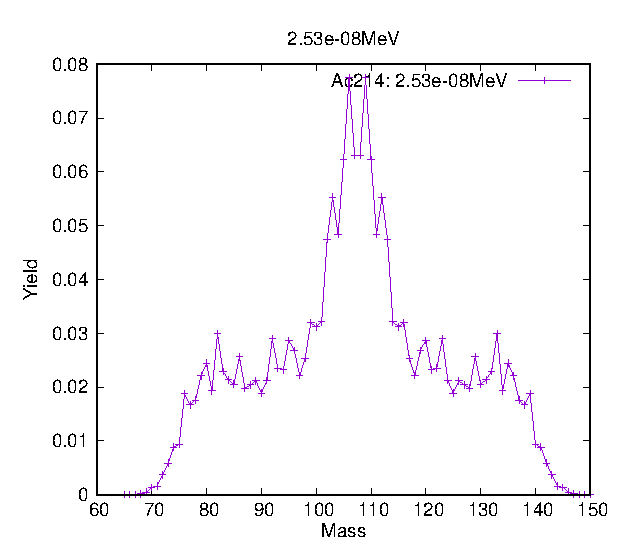
\includegraphics[width=\textwidth]{YA/Ac214_2.53e-08.eps} \end{center} \end{minipage}
\begin{minipage}{0.33\textwidth} \begin{center} 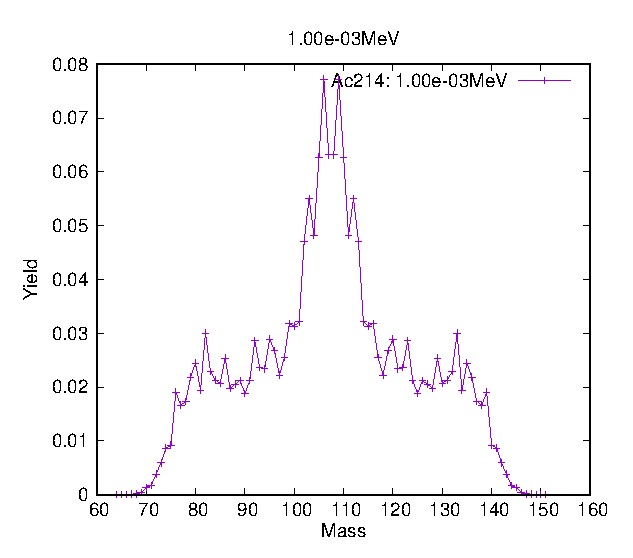
\includegraphics[width=\textwidth]{YA/Ac214_1.00e-03.eps} \end{center} \end{minipage}
\begin{minipage}{0.33\textwidth} \begin{center} 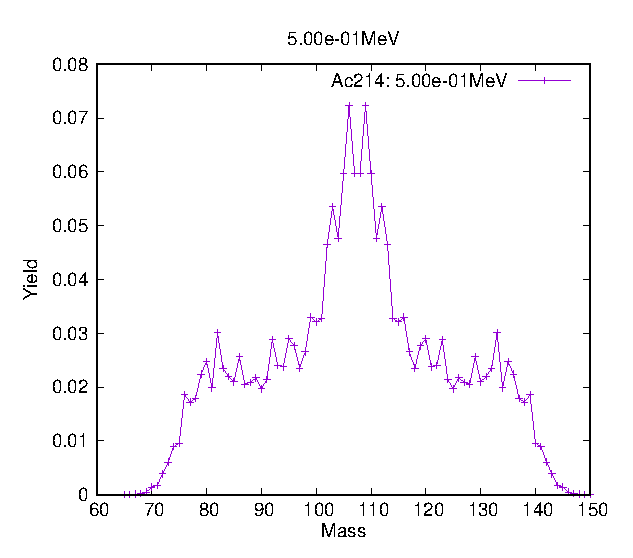
\includegraphics[width=\textwidth]{YA/Ac214_5.00e-01.eps} \end{center} \end{minipage}
\end{figure}
\begin{figure}[htbp]
 \begin{minipage}{0.33\textwidth} \begin{center} 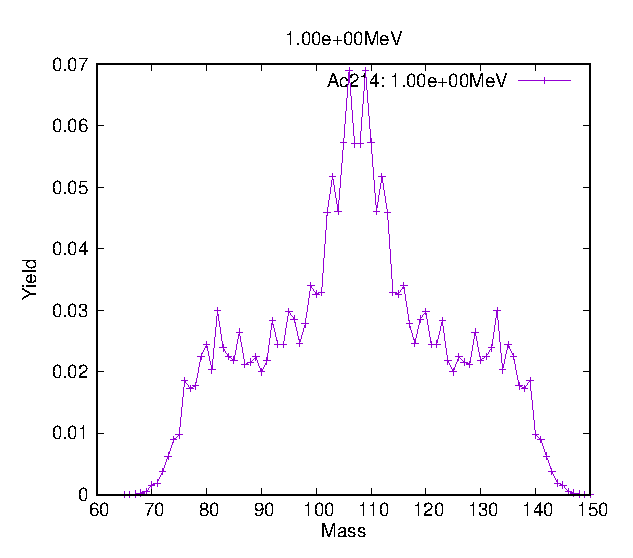
\includegraphics[width=\textwidth]{YA/Ac214_1.00e+00.eps} \end{center} \end{minipage}
\begin{minipage}{0.33\textwidth} \begin{center} 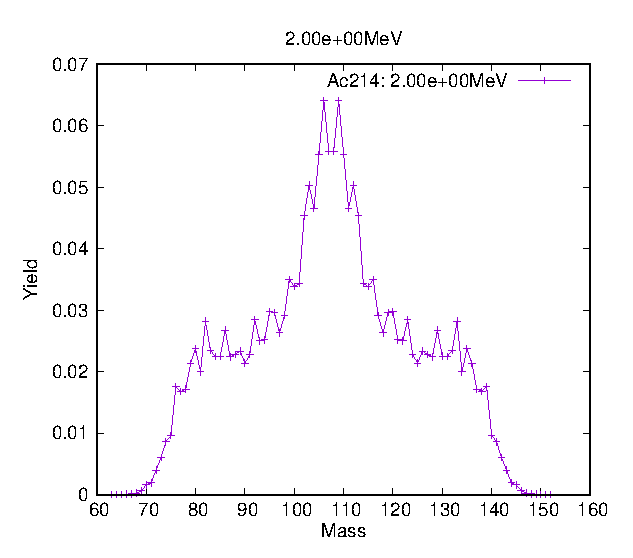
\includegraphics[width=\textwidth]{YA/Ac214_2.00e+00.eps} \end{center} \end{minipage}
\begin{minipage}{0.33\textwidth} \begin{center} 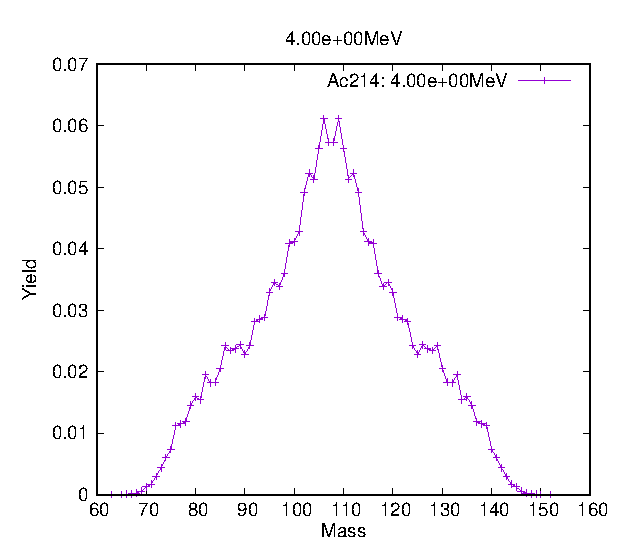
\includegraphics[width=\textwidth]{YA/Ac214_4.00e+00.eps} \end{center} \end{minipage}
\end{figure}
\begin{figure}[htbp]
 \begin{minipage}{0.33\textwidth} \begin{center} 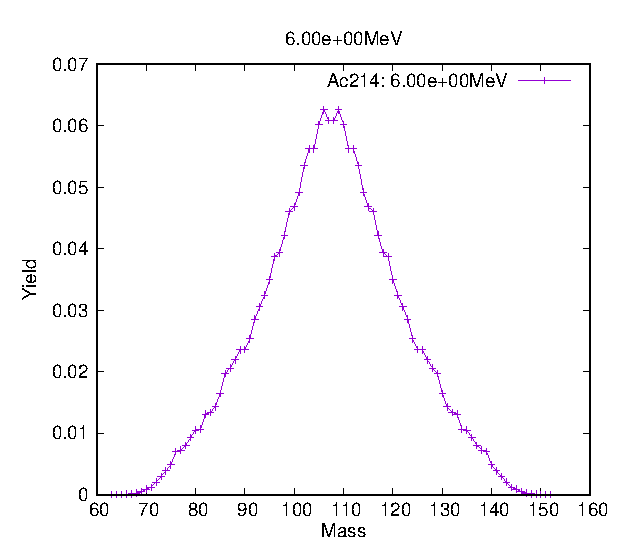
\includegraphics[width=\textwidth]{YA/Ac214_6.00e+00.eps} \end{center} \end{minipage}
\begin{minipage}{0.33\textwidth} \begin{center} 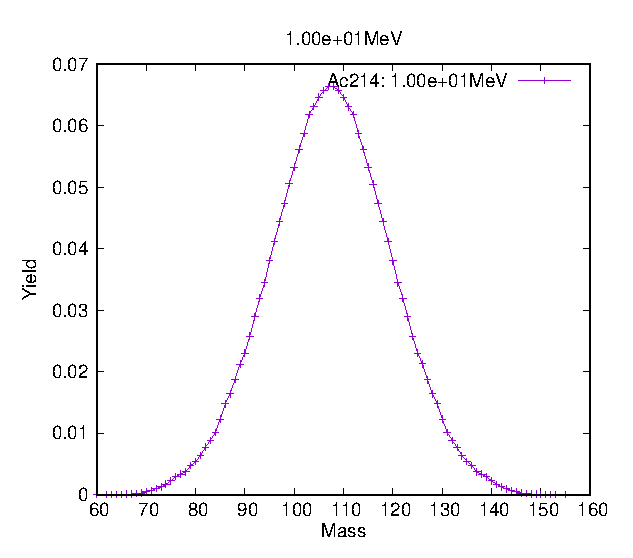
\includegraphics[width=\textwidth]{YA/Ac214_1.00e+01.eps} \end{center} \end{minipage}
\begin{minipage}{0.33\textwidth} \begin{center} 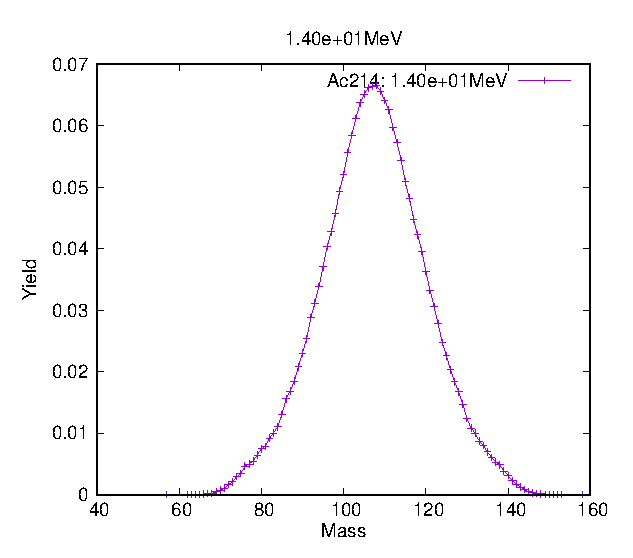
\includegraphics[width=\textwidth]{YA/Ac214_1.40e+01.eps} \end{center} \end{minipage}
\end{figure}
\clearpage

 
\section{Ac222}
\begin{figure}[htbp]
 \begin{minipage}{0.33\textwidth} \begin{center} 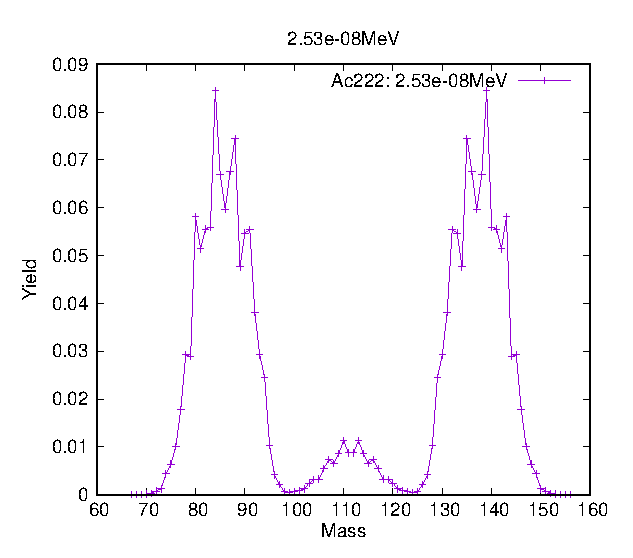
\includegraphics[width=\textwidth]{YA/Ac222_2.53e-08.eps} \end{center} \end{minipage}
\begin{minipage}{0.33\textwidth} \begin{center} 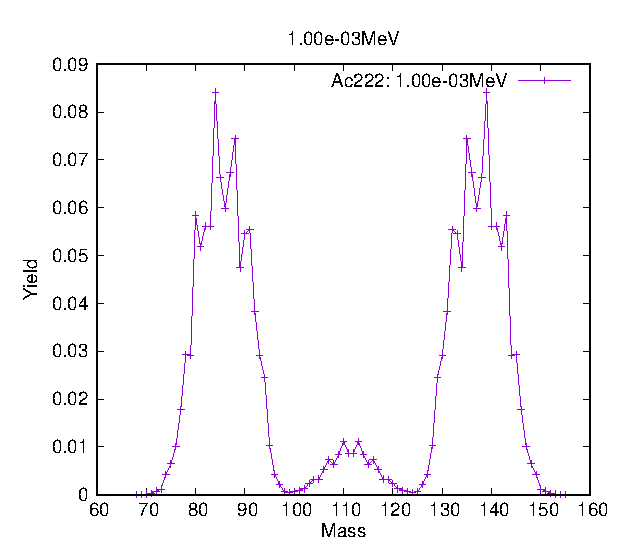
\includegraphics[width=\textwidth]{YA/Ac222_1.00e-03.eps} \end{center} \end{minipage}
\begin{minipage}{0.33\textwidth} \begin{center} 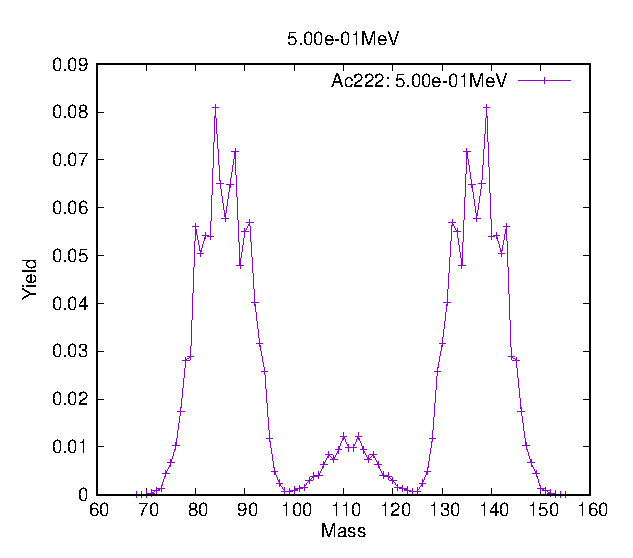
\includegraphics[width=\textwidth]{YA/Ac222_5.00e-01.eps} \end{center} \end{minipage}
\end{figure}
\begin{figure}[htbp]
 \begin{minipage}{0.33\textwidth} \begin{center} 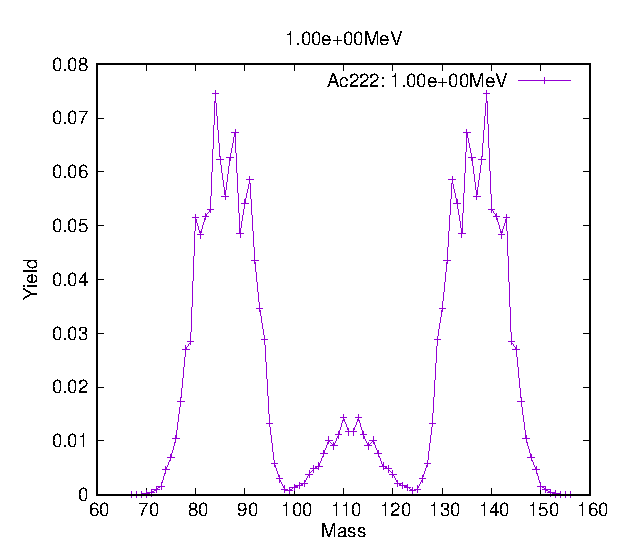
\includegraphics[width=\textwidth]{YA/Ac222_1.00e+00.eps} \end{center} \end{minipage}
\begin{minipage}{0.33\textwidth} \begin{center} 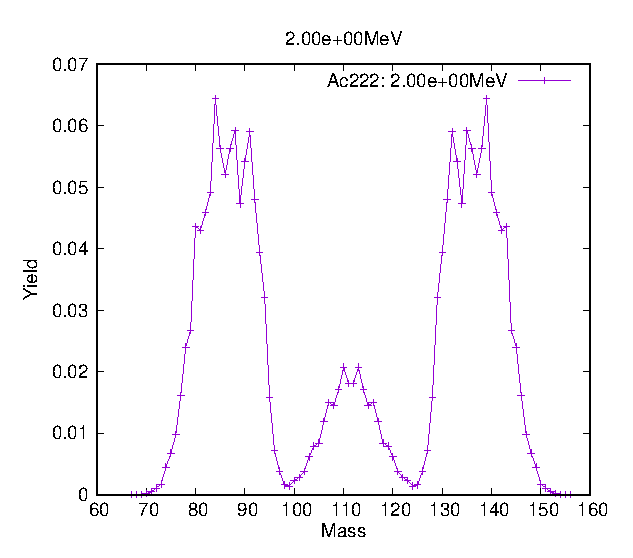
\includegraphics[width=\textwidth]{YA/Ac222_2.00e+00.eps} \end{center} \end{minipage}
\begin{minipage}{0.33\textwidth} \begin{center} 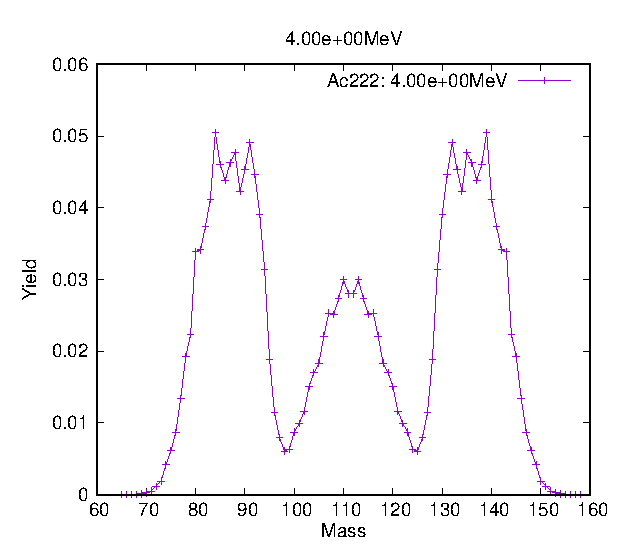
\includegraphics[width=\textwidth]{YA/Ac222_4.00e+00.eps} \end{center} \end{minipage}
\end{figure}
\begin{figure}[htbp]
 \begin{minipage}{0.33\textwidth} \begin{center} 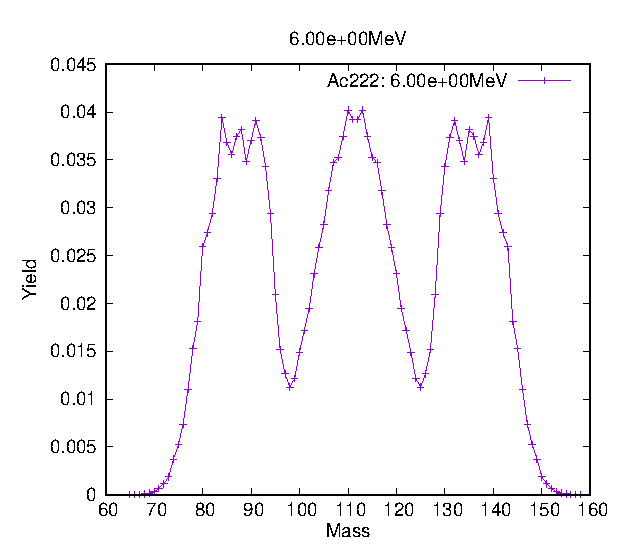
\includegraphics[width=\textwidth]{YA/Ac222_6.00e+00.eps} \end{center} \end{minipage}
\begin{minipage}{0.33\textwidth} \begin{center} 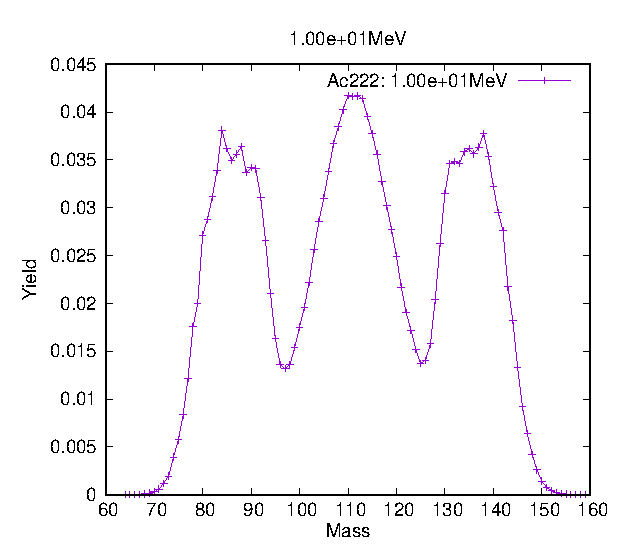
\includegraphics[width=\textwidth]{YA/Ac222_1.00e+01.eps} \end{center} \end{minipage}
\begin{minipage}{0.33\textwidth} \begin{center} 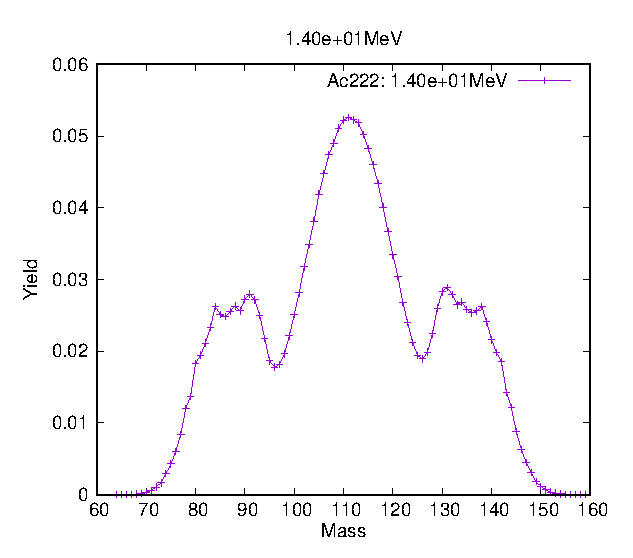
\includegraphics[width=\textwidth]{YA/Ac222_1.40e+01.eps} \end{center} \end{minipage}
\end{figure}
\clearpage

 
\section{Ac223}
\begin{figure}[htbp]
 \begin{minipage}{0.33\textwidth} \begin{center} 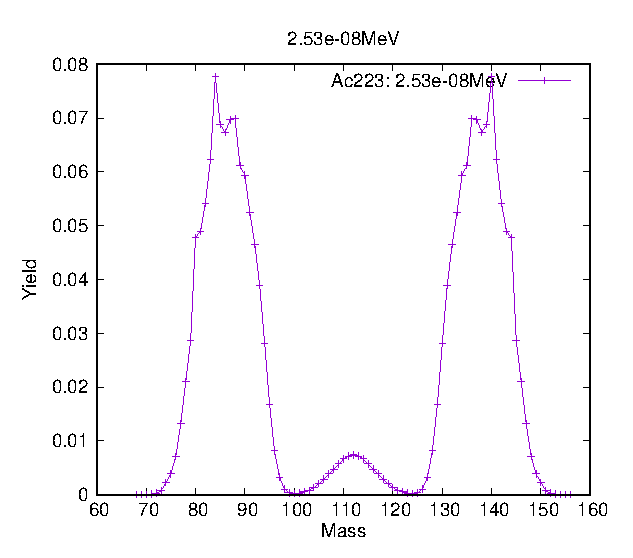
\includegraphics[width=\textwidth]{YA/Ac223_2.53e-08.eps} \end{center} \end{minipage}
\begin{minipage}{0.33\textwidth} \begin{center} 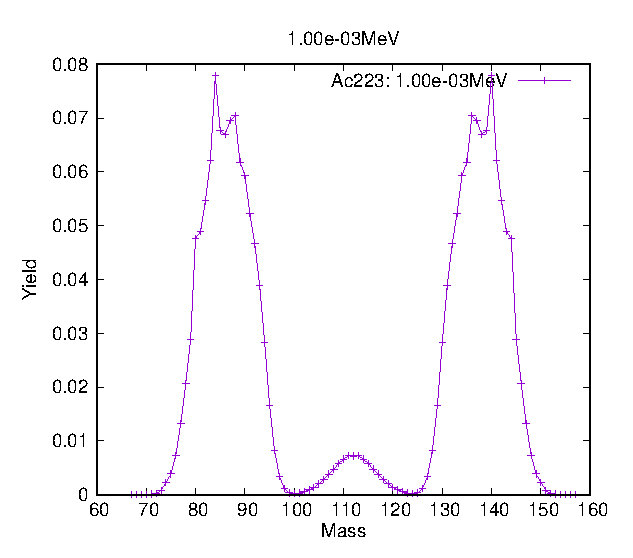
\includegraphics[width=\textwidth]{YA/Ac223_1.00e-03.eps} \end{center} \end{minipage}
\begin{minipage}{0.33\textwidth} \begin{center} 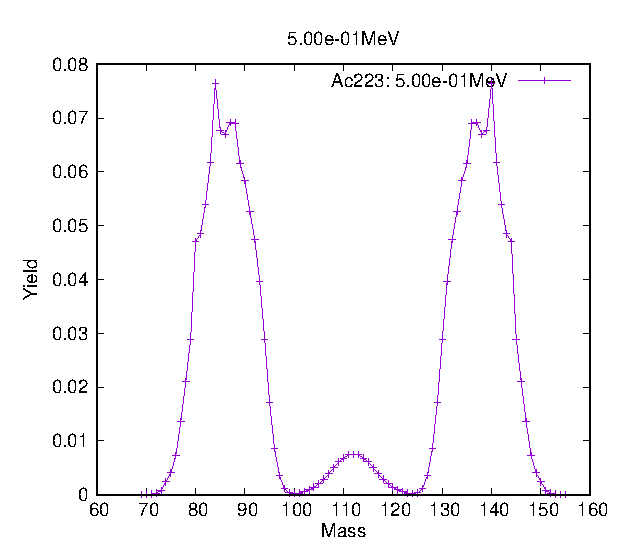
\includegraphics[width=\textwidth]{YA/Ac223_5.00e-01.eps} \end{center} \end{minipage}
\end{figure}
\begin{figure}[htbp]
 \begin{minipage}{0.33\textwidth} \begin{center} 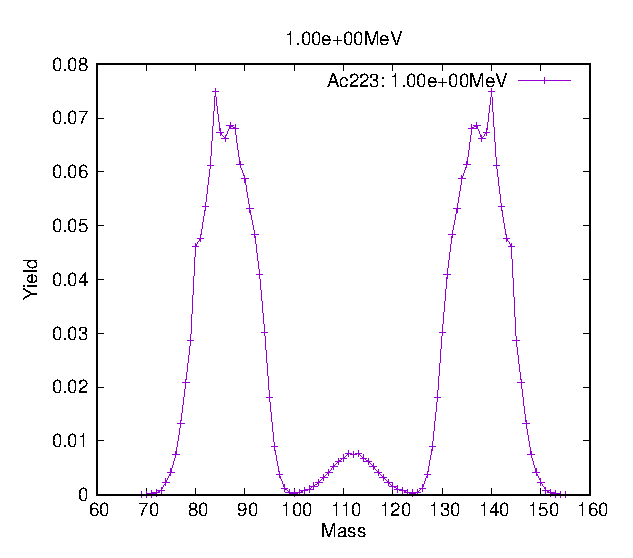
\includegraphics[width=\textwidth]{YA/Ac223_1.00e+00.eps} \end{center} \end{minipage}
\begin{minipage}{0.33\textwidth} \begin{center} 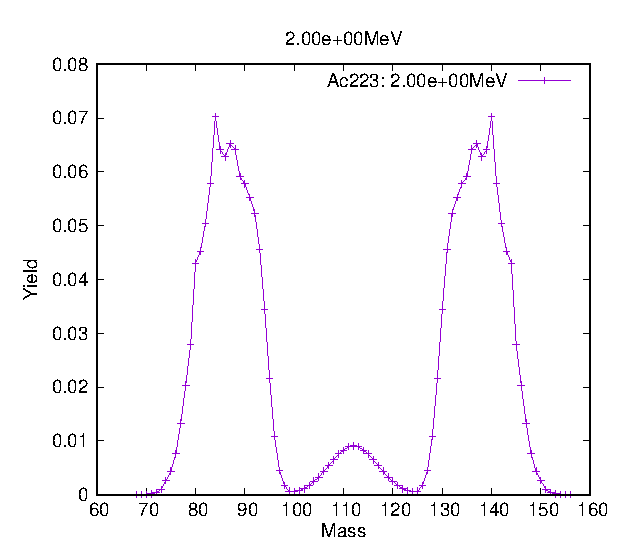
\includegraphics[width=\textwidth]{YA/Ac223_2.00e+00.eps} \end{center} \end{minipage}
\begin{minipage}{0.33\textwidth} \begin{center} 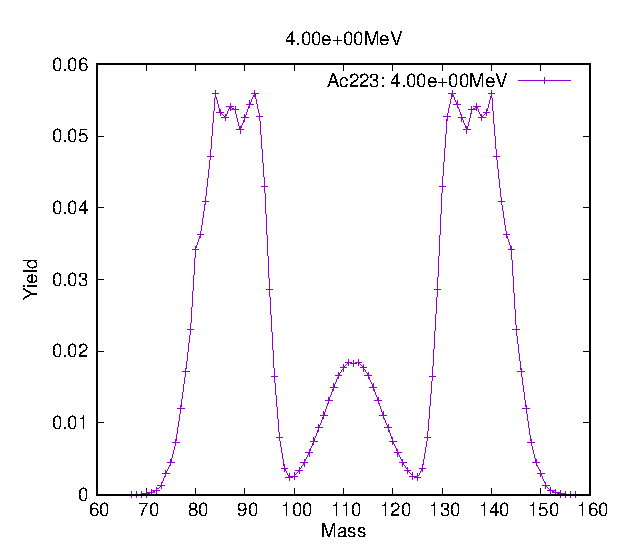
\includegraphics[width=\textwidth]{YA/Ac223_4.00e+00.eps} \end{center} \end{minipage}
\end{figure}
\begin{figure}[htbp]
 \begin{minipage}{0.33\textwidth} \begin{center} 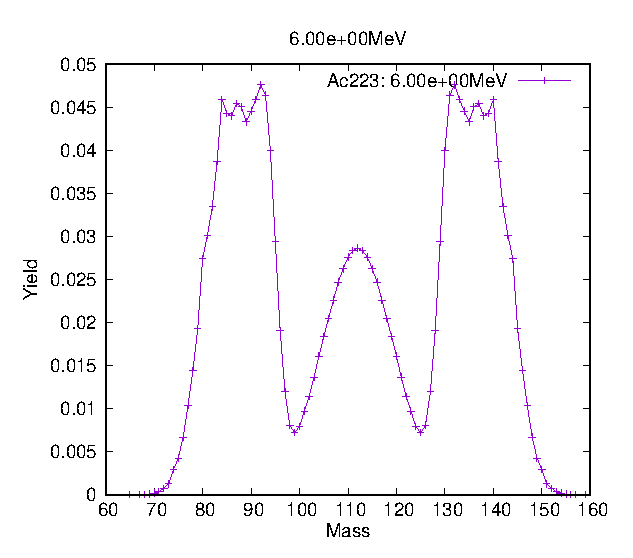
\includegraphics[width=\textwidth]{YA/Ac223_6.00e+00.eps} \end{center} \end{minipage}
\begin{minipage}{0.33\textwidth} \begin{center} 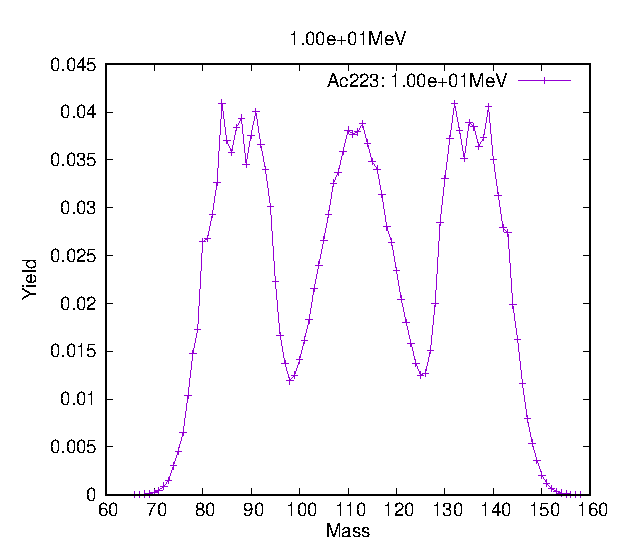
\includegraphics[width=\textwidth]{YA/Ac223_1.00e+01.eps} \end{center} \end{minipage}
\begin{minipage}{0.33\textwidth} \begin{center} 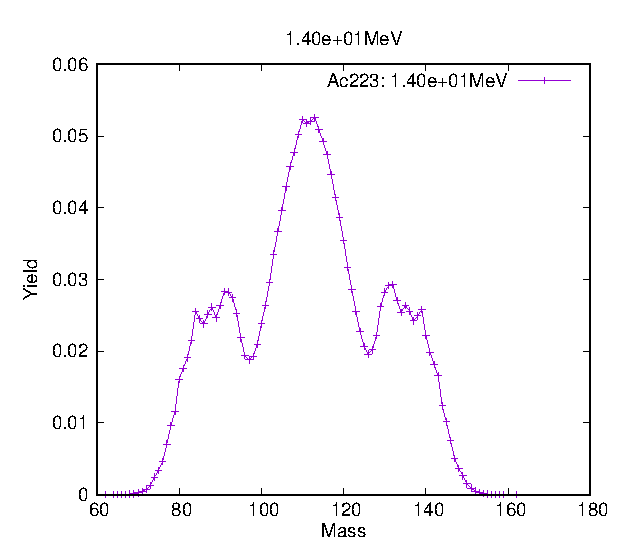
\includegraphics[width=\textwidth]{YA/Ac223_1.40e+01.eps} \end{center} \end{minipage}
\end{figure}
\clearpage

 
\section{Ac224}
\begin{figure}[htbp]
 \begin{minipage}{0.33\textwidth} \begin{center} 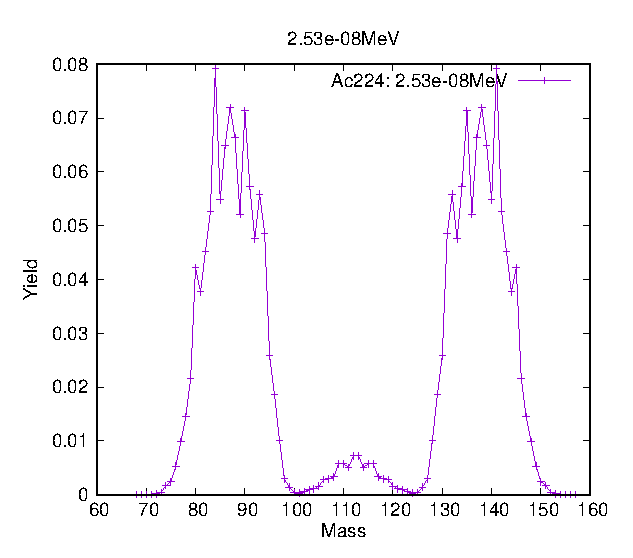
\includegraphics[width=\textwidth]{YA/Ac224_2.53e-08.eps} \end{center} \end{minipage}
\begin{minipage}{0.33\textwidth} \begin{center} 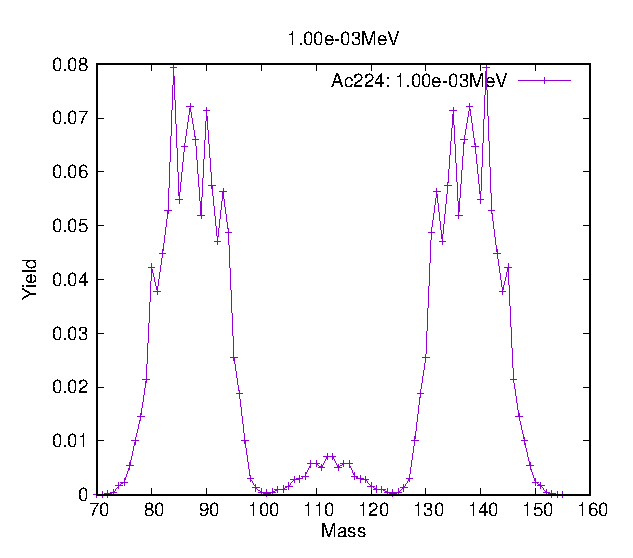
\includegraphics[width=\textwidth]{YA/Ac224_1.00e-03.eps} \end{center} \end{minipage}
\begin{minipage}{0.33\textwidth} \begin{center} 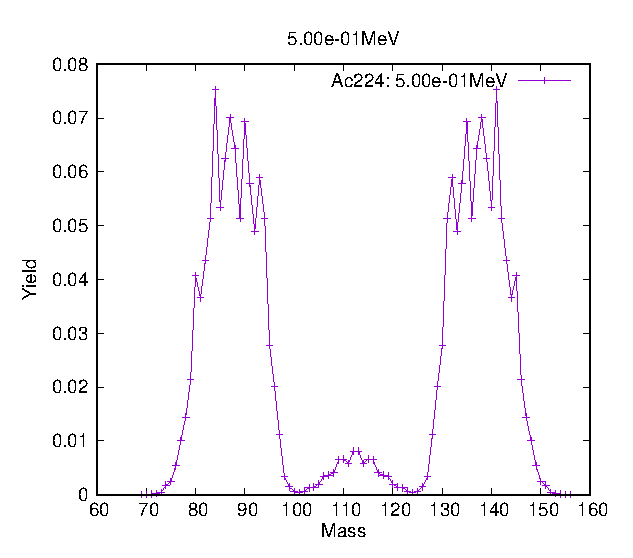
\includegraphics[width=\textwidth]{YA/Ac224_5.00e-01.eps} \end{center} \end{minipage}
\end{figure}
\begin{figure}[htbp]
 \begin{minipage}{0.33\textwidth} \begin{center} 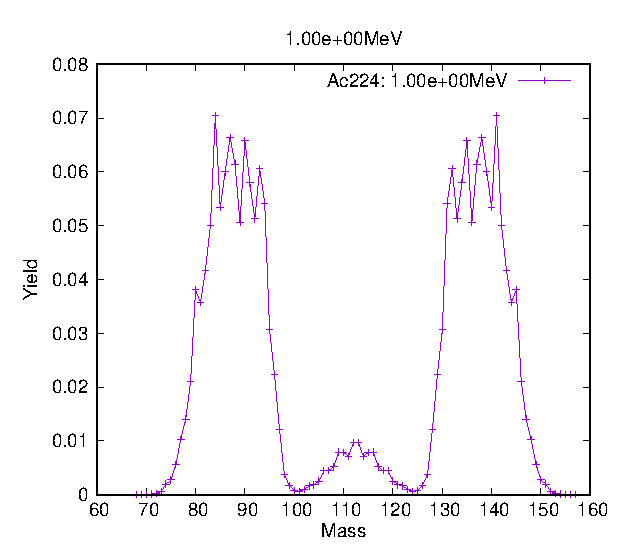
\includegraphics[width=\textwidth]{YA/Ac224_1.00e+00.eps} \end{center} \end{minipage}
\begin{minipage}{0.33\textwidth} \begin{center} 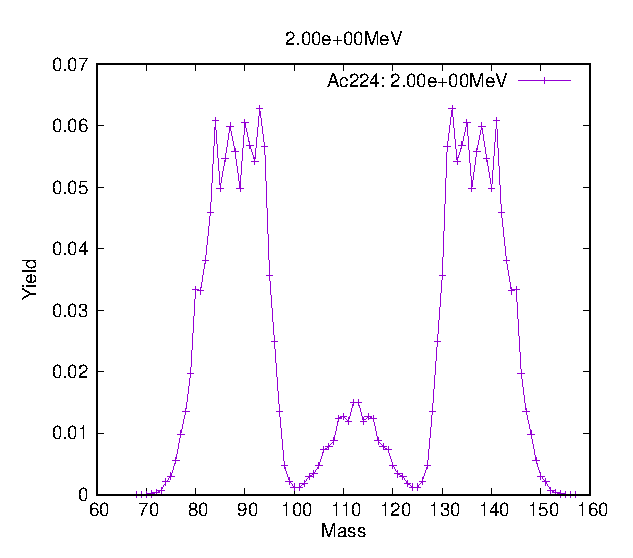
\includegraphics[width=\textwidth]{YA/Ac224_2.00e+00.eps} \end{center} \end{minipage}
\begin{minipage}{0.33\textwidth} \begin{center} 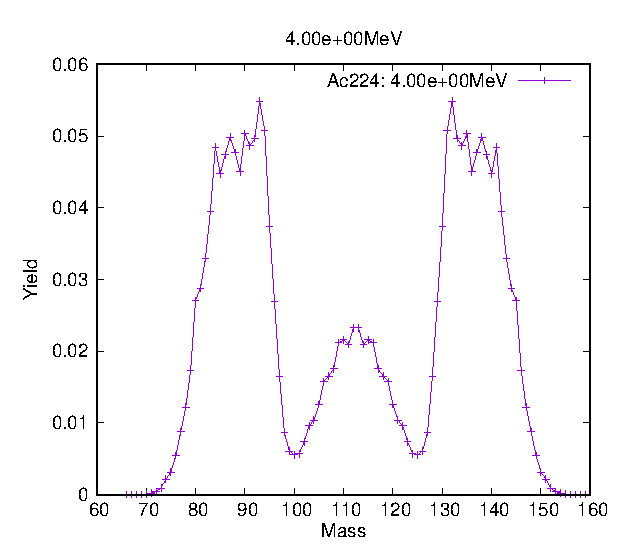
\includegraphics[width=\textwidth]{YA/Ac224_4.00e+00.eps} \end{center} \end{minipage}
\end{figure}
\begin{figure}[htbp]
 \begin{minipage}{0.33\textwidth} \begin{center} 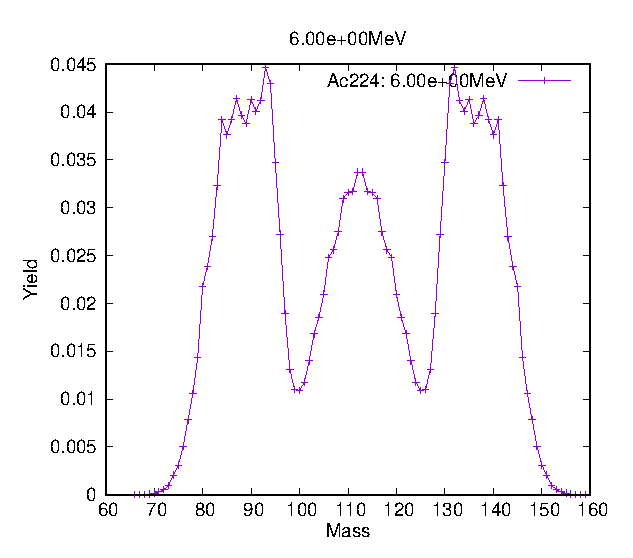
\includegraphics[width=\textwidth]{YA/Ac224_6.00e+00.eps} \end{center} \end{minipage}
\begin{minipage}{0.33\textwidth} \begin{center} 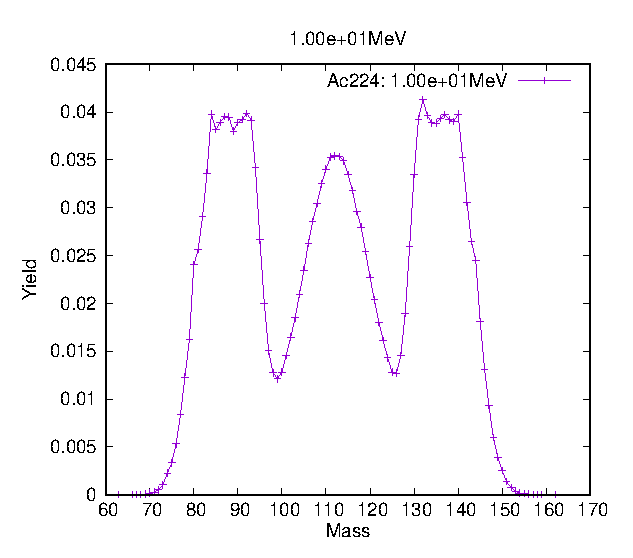
\includegraphics[width=\textwidth]{YA/Ac224_1.00e+01.eps} \end{center} \end{minipage}
\begin{minipage}{0.33\textwidth} \begin{center} 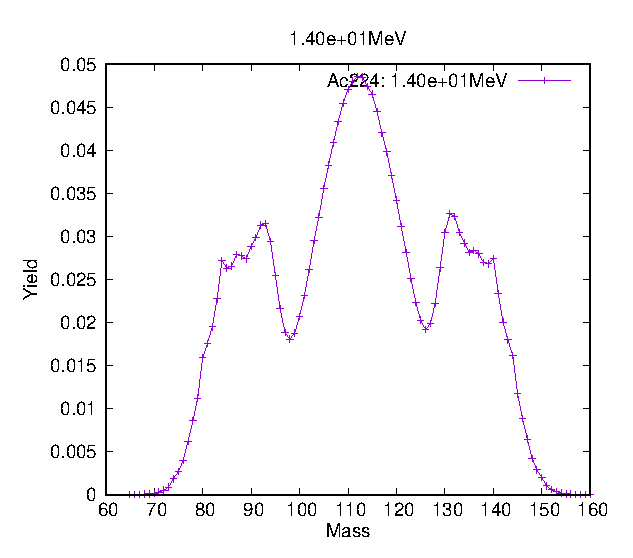
\includegraphics[width=\textwidth]{YA/Ac224_1.40e+01.eps} \end{center} \end{minipage}
\end{figure}
\clearpage

 
\section{Ac225}
\begin{figure}[htbp]
 \begin{minipage}{0.33\textwidth} \begin{center} 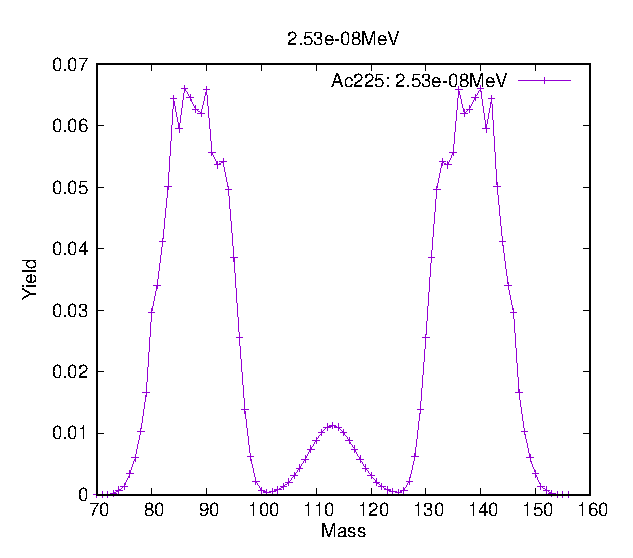
\includegraphics[width=\textwidth]{YA/Ac225_2.53e-08.eps} \end{center} \end{minipage}
\begin{minipage}{0.33\textwidth} \begin{center} 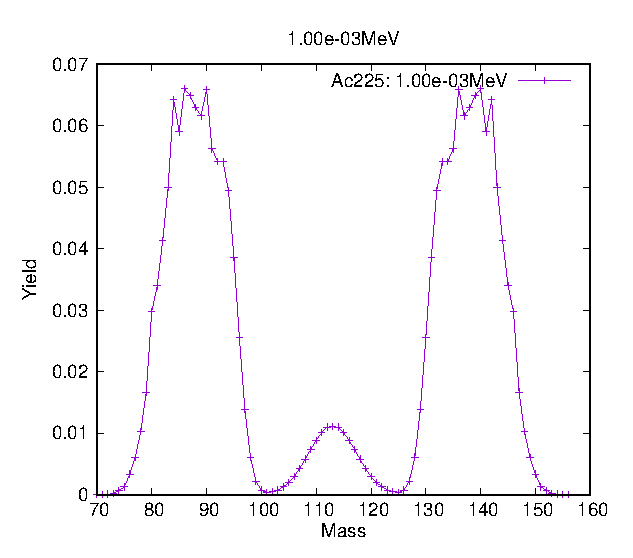
\includegraphics[width=\textwidth]{YA/Ac225_1.00e-03.eps} \end{center} \end{minipage}
\begin{minipage}{0.33\textwidth} \begin{center} 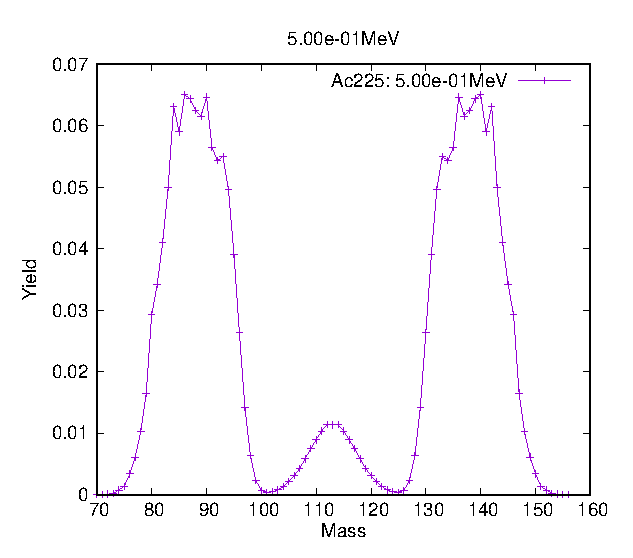
\includegraphics[width=\textwidth]{YA/Ac225_5.00e-01.eps} \end{center} \end{minipage}
\end{figure}
\begin{figure}[htbp]
 \begin{minipage}{0.33\textwidth} \begin{center} 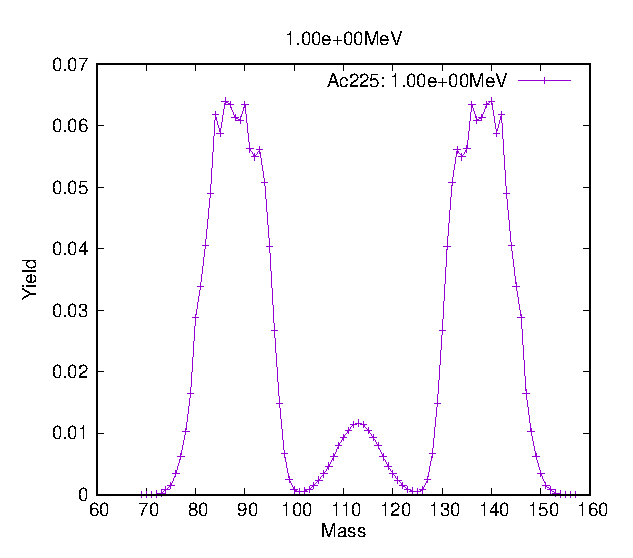
\includegraphics[width=\textwidth]{YA/Ac225_1.00e+00.eps} \end{center} \end{minipage}
\begin{minipage}{0.33\textwidth} \begin{center} 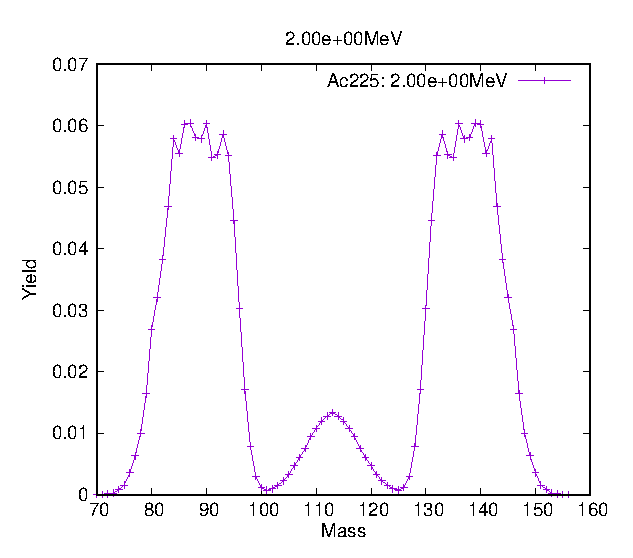
\includegraphics[width=\textwidth]{YA/Ac225_2.00e+00.eps} \end{center} \end{minipage}
\begin{minipage}{0.33\textwidth} \begin{center} 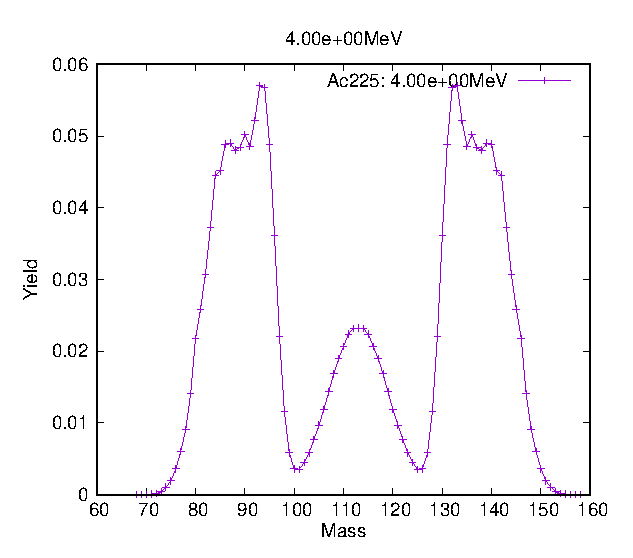
\includegraphics[width=\textwidth]{YA/Ac225_4.00e+00.eps} \end{center} \end{minipage}
\end{figure}
\begin{figure}[htbp]
 \begin{minipage}{0.33\textwidth} \begin{center} 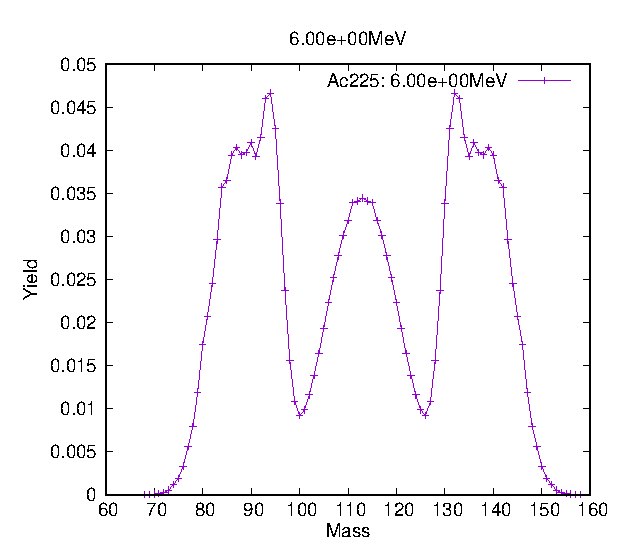
\includegraphics[width=\textwidth]{YA/Ac225_6.00e+00.eps} \end{center} \end{minipage}
\begin{minipage}{0.33\textwidth} \begin{center} 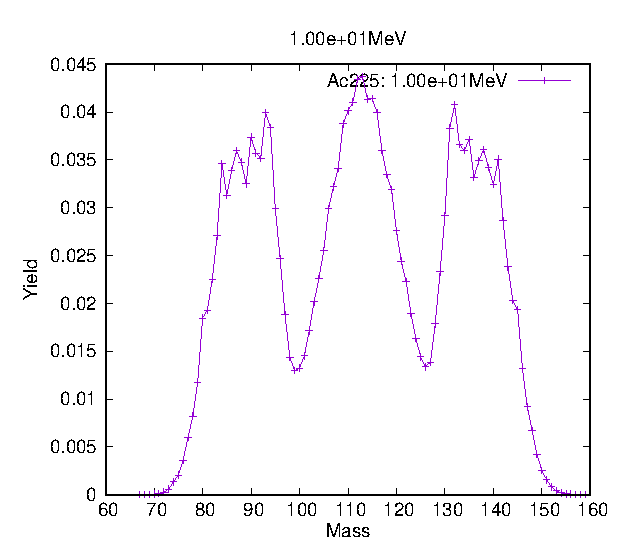
\includegraphics[width=\textwidth]{YA/Ac225_1.00e+01.eps} \end{center} \end{minipage}
\begin{minipage}{0.33\textwidth} \begin{center} 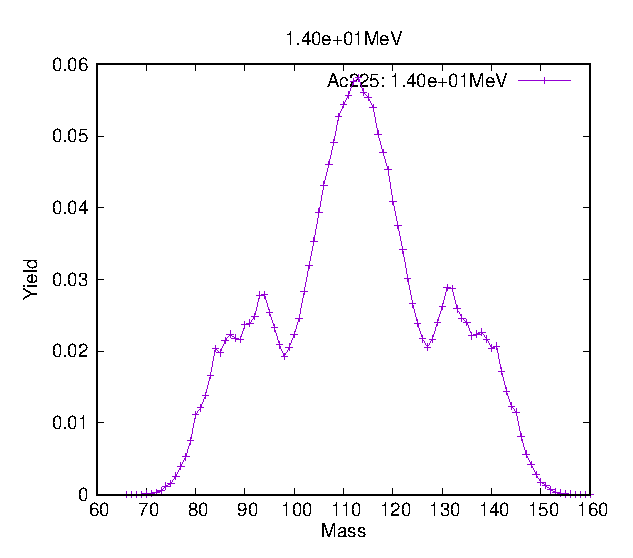
\includegraphics[width=\textwidth]{YA/Ac225_1.40e+01.eps} \end{center} \end{minipage}
\end{figure}
\clearpage

 
\section{Ac226}
\begin{figure}[htbp]
 \begin{minipage}{0.33\textwidth} \begin{center} 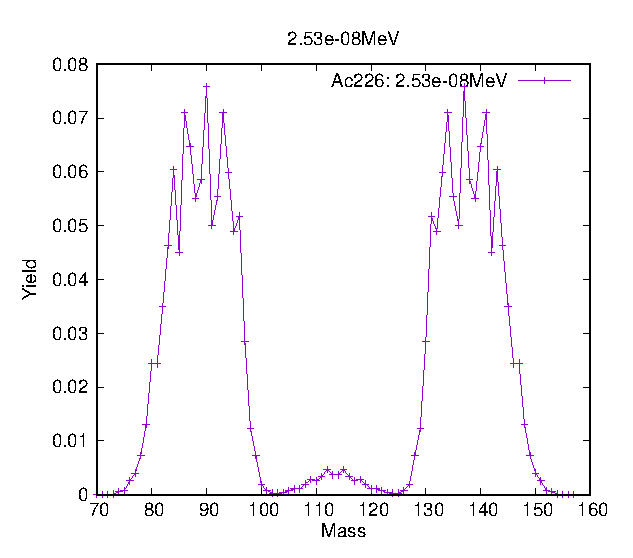
\includegraphics[width=\textwidth]{YA/Ac226_2.53e-08.eps} \end{center} \end{minipage}
\begin{minipage}{0.33\textwidth} \begin{center} 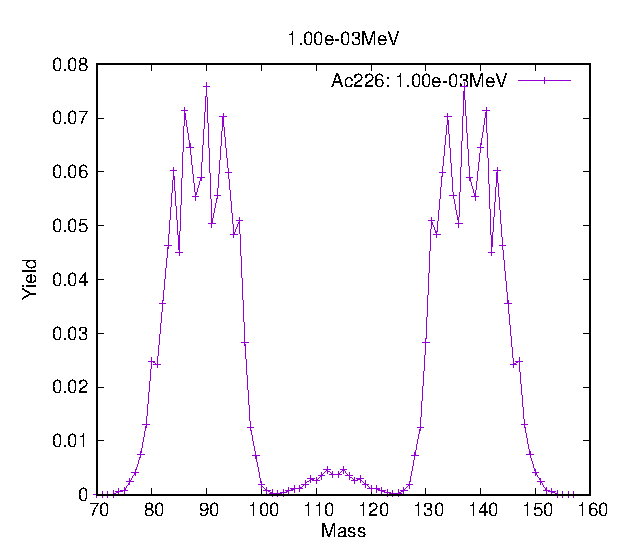
\includegraphics[width=\textwidth]{YA/Ac226_1.00e-03.eps} \end{center} \end{minipage}
\begin{minipage}{0.33\textwidth} \begin{center} 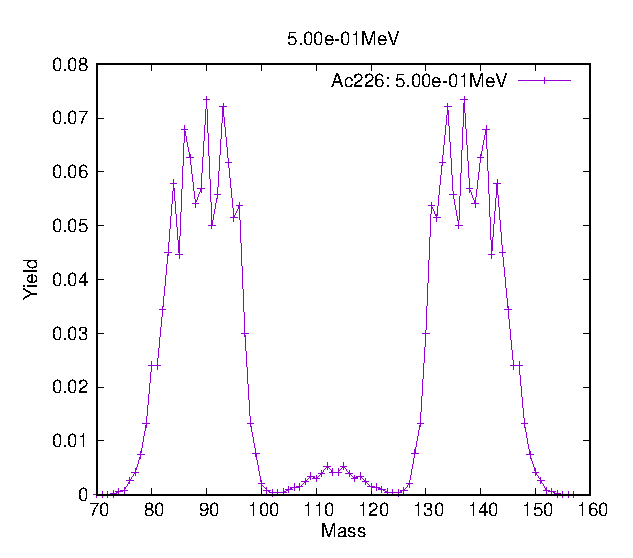
\includegraphics[width=\textwidth]{YA/Ac226_5.00e-01.eps} \end{center} \end{minipage}
\end{figure}
\begin{figure}[htbp]
 \begin{minipage}{0.33\textwidth} \begin{center} 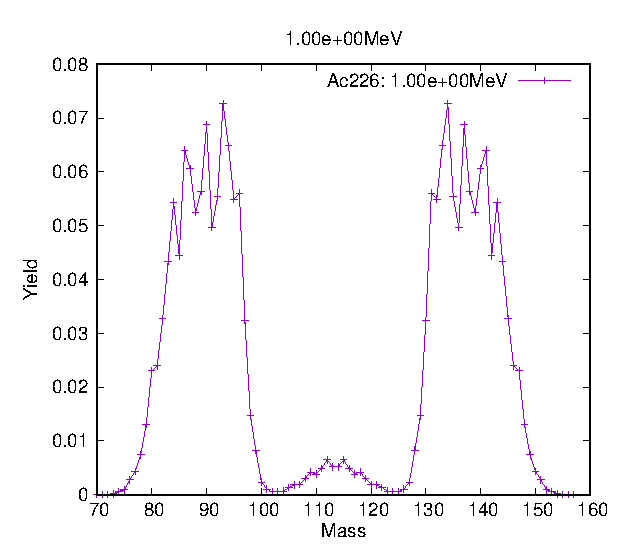
\includegraphics[width=\textwidth]{YA/Ac226_1.00e+00.eps} \end{center} \end{minipage}
\begin{minipage}{0.33\textwidth} \begin{center} 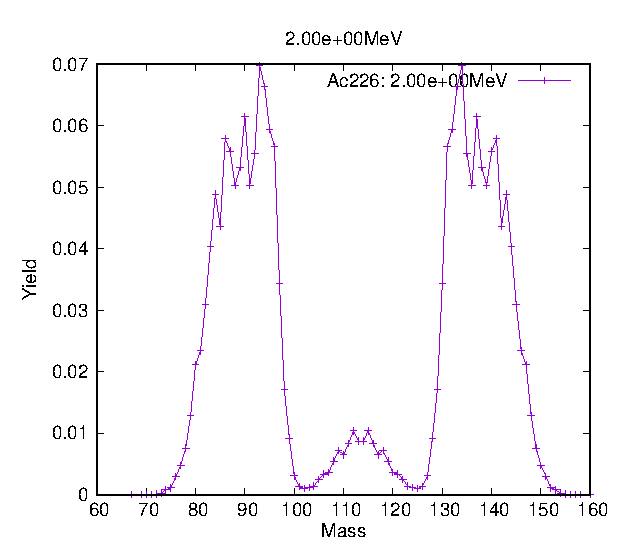
\includegraphics[width=\textwidth]{YA/Ac226_2.00e+00.eps} \end{center} \end{minipage}
\begin{minipage}{0.33\textwidth} \begin{center} \includegraphics[width=\textwidth]{YA/Ac226_4.00e+00.eps} \end{center} \end{minipage}
\end{figure}
\begin{figure}[htbp]
 \begin{minipage}{0.33\textwidth} \begin{center} \includegraphics[width=\textwidth]{YA/Ac226_6.00e+00.eps} \end{center} \end{minipage}
\begin{minipage}{0.33\textwidth} \begin{center} \includegraphics[width=\textwidth]{YA/Ac226_1.00e+01.eps} \end{center} \end{minipage}
\begin{minipage}{0.33\textwidth} \begin{center} \includegraphics[width=\textwidth]{YA/Ac226_1.40e+01.eps} \end{center} \end{minipage}
\end{figure}
\clearpage

 
\section{Ac227}
\begin{figure}[htbp]
 \begin{minipage}{0.33\textwidth} \begin{center} \includegraphics[width=\textwidth]{YA/Ac227_2.53e-08.eps} \end{center} \end{minipage}
\begin{minipage}{0.33\textwidth} \begin{center} \includegraphics[width=\textwidth]{YA/Ac227_1.00e-03.eps} \end{center} \end{minipage}
\begin{minipage}{0.33\textwidth} \begin{center} \includegraphics[width=\textwidth]{YA/Ac227_5.00e-01.eps} \end{center} \end{minipage}
\end{figure}
\begin{figure}[htbp]
 \begin{minipage}{0.33\textwidth} \begin{center} \includegraphics[width=\textwidth]{YA/Ac227_1.00e+00.eps} \end{center} \end{minipage}
\begin{minipage}{0.33\textwidth} \begin{center} \includegraphics[width=\textwidth]{YA/Ac227_2.00e+00.eps} \end{center} \end{minipage}
\begin{minipage}{0.33\textwidth} \begin{center} \includegraphics[width=\textwidth]{YA/Ac227_4.00e+00.eps} \end{center} \end{minipage}
\end{figure}
\begin{figure}[htbp]
 \begin{minipage}{0.33\textwidth} \begin{center} \includegraphics[width=\textwidth]{YA/Ac227_6.00e+00.eps} \end{center} \end{minipage}
\begin{minipage}{0.33\textwidth} \begin{center} \includegraphics[width=\textwidth]{YA/Ac227_1.00e+01.eps} \end{center} \end{minipage}
\begin{minipage}{0.33\textwidth} \begin{center} \includegraphics[width=\textwidth]{YA/Ac227_1.40e+01.eps} \end{center} \end{minipage}
\end{figure}
\clearpage

 
\section{Ac228}
\begin{figure}[htbp]
 \begin{minipage}{0.33\textwidth} \begin{center} \includegraphics[width=\textwidth]{YA/Ac228_2.53e-08.eps} \end{center} \end{minipage}
\begin{minipage}{0.33\textwidth} \begin{center} \includegraphics[width=\textwidth]{YA/Ac228_1.00e-03.eps} \end{center} \end{minipage}
\begin{minipage}{0.33\textwidth} \begin{center} \includegraphics[width=\textwidth]{YA/Ac228_5.00e-01.eps} \end{center} \end{minipage}
\end{figure}
\begin{figure}[htbp]
 \begin{minipage}{0.33\textwidth} \begin{center} \includegraphics[width=\textwidth]{YA/Ac228_1.00e+00.eps} \end{center} \end{minipage}
\begin{minipage}{0.33\textwidth} \begin{center} \includegraphics[width=\textwidth]{YA/Ac228_2.00e+00.eps} \end{center} \end{minipage}
\begin{minipage}{0.33\textwidth} \begin{center} \includegraphics[width=\textwidth]{YA/Ac228_4.00e+00.eps} \end{center} \end{minipage}
\end{figure}
\begin{figure}[htbp]
 \begin{minipage}{0.33\textwidth} \begin{center} \includegraphics[width=\textwidth]{YA/Ac228_6.00e+00.eps} \end{center} \end{minipage}
\begin{minipage}{0.33\textwidth} \begin{center} \includegraphics[width=\textwidth]{YA/Ac228_1.00e+01.eps} \end{center} \end{minipage}
\begin{minipage}{0.33\textwidth} \begin{center} \includegraphics[width=\textwidth]{YA/Ac228_1.40e+01.eps} \end{center} \end{minipage}
\end{figure}
\clearpage

 
\section{Ac229}
\begin{figure}[htbp]
 \begin{minipage}{0.33\textwidth} \begin{center} \includegraphics[width=\textwidth]{YA/Ac229_2.53e-08.eps} \end{center} \end{minipage}
\begin{minipage}{0.33\textwidth} \begin{center} \includegraphics[width=\textwidth]{YA/Ac229_1.00e-03.eps} \end{center} \end{minipage}
\begin{minipage}{0.33\textwidth} \begin{center} \includegraphics[width=\textwidth]{YA/Ac229_5.00e-01.eps} \end{center} \end{minipage}
\end{figure}
\begin{figure}[htbp]
 \begin{minipage}{0.33\textwidth} \begin{center} \includegraphics[width=\textwidth]{YA/Ac229_1.00e+00.eps} \end{center} \end{minipage}
\begin{minipage}{0.33\textwidth} \begin{center} \includegraphics[width=\textwidth]{YA/Ac229_2.00e+00.eps} \end{center} \end{minipage}
\begin{minipage}{0.33\textwidth} \begin{center} \includegraphics[width=\textwidth]{YA/Ac229_4.00e+00.eps} \end{center} \end{minipage}
\end{figure}
\begin{figure}[htbp]
 \begin{minipage}{0.33\textwidth} \begin{center} \includegraphics[width=\textwidth]{YA/Ac229_6.00e+00.eps} \end{center} \end{minipage}
\begin{minipage}{0.33\textwidth} \begin{center} \includegraphics[width=\textwidth]{YA/Ac229_1.00e+01.eps} \end{center} \end{minipage}
\begin{minipage}{0.33\textwidth} \begin{center} \includegraphics[width=\textwidth]{YA/Ac229_1.40e+01.eps} \end{center} \end{minipage}
\end{figure}
\clearpage

 
\section{Ac230}
\begin{figure}[htbp]
 \begin{minipage}{0.33\textwidth} \begin{center} \includegraphics[width=\textwidth]{YA/Ac230_2.53e-08.eps} \end{center} \end{minipage}
\begin{minipage}{0.33\textwidth} \begin{center} \includegraphics[width=\textwidth]{YA/Ac230_1.00e-03.eps} \end{center} \end{minipage}
\begin{minipage}{0.33\textwidth} \begin{center} \includegraphics[width=\textwidth]{YA/Ac230_5.00e-01.eps} \end{center} \end{minipage}
\end{figure}
\begin{figure}[htbp]
 \begin{minipage}{0.33\textwidth} \begin{center} \includegraphics[width=\textwidth]{YA/Ac230_1.00e+00.eps} \end{center} \end{minipage}
\begin{minipage}{0.33\textwidth} \begin{center} \includegraphics[width=\textwidth]{YA/Ac230_2.00e+00.eps} \end{center} \end{minipage}
\begin{minipage}{0.33\textwidth} \begin{center} \includegraphics[width=\textwidth]{YA/Ac230_4.00e+00.eps} \end{center} \end{minipage}
\end{figure}
\begin{figure}[htbp]
 \begin{minipage}{0.33\textwidth} \begin{center} \includegraphics[width=\textwidth]{YA/Ac230_6.00e+00.eps} \end{center} \end{minipage}
\begin{minipage}{0.33\textwidth} \begin{center} \includegraphics[width=\textwidth]{YA/Ac230_1.00e+01.eps} \end{center} \end{minipage}
\begin{minipage}{0.33\textwidth} \begin{center} \includegraphics[width=\textwidth]{YA/Ac230_1.40e+01.eps} \end{center} \end{minipage}
\end{figure}
\clearpage

 
\section{Ac231}
\begin{figure}[htbp]
 \begin{minipage}{0.33\textwidth} \begin{center} \includegraphics[width=\textwidth]{YA/Ac231_2.53e-08.eps} \end{center} \end{minipage}
\begin{minipage}{0.33\textwidth} \begin{center} \includegraphics[width=\textwidth]{YA/Ac231_1.00e-03.eps} \end{center} \end{minipage}
\begin{minipage}{0.33\textwidth} \begin{center} \includegraphics[width=\textwidth]{YA/Ac231_5.00e-01.eps} \end{center} \end{minipage}
\end{figure}
\begin{figure}[htbp]
 \begin{minipage}{0.33\textwidth} \begin{center} \includegraphics[width=\textwidth]{YA/Ac231_1.00e+00.eps} \end{center} \end{minipage}
\begin{minipage}{0.33\textwidth} \begin{center} \includegraphics[width=\textwidth]{YA/Ac231_2.00e+00.eps} \end{center} \end{minipage}
\begin{minipage}{0.33\textwidth} \begin{center} \includegraphics[width=\textwidth]{YA/Ac231_4.00e+00.eps} \end{center} \end{minipage}
\end{figure}
\begin{figure}[htbp]
 \begin{minipage}{0.33\textwidth} \begin{center} \includegraphics[width=\textwidth]{YA/Ac231_6.00e+00.eps} \end{center} \end{minipage}
\begin{minipage}{0.33\textwidth} \begin{center} \includegraphics[width=\textwidth]{YA/Ac231_1.00e+01.eps} \end{center} \end{minipage}
\begin{minipage}{0.33\textwidth} \begin{center} \includegraphics[width=\textwidth]{YA/Ac231_1.40e+01.eps} \end{center} \end{minipage}
\end{figure}
\clearpage

 
\section{Ac232}
\begin{figure}[htbp]
 \begin{minipage}{0.33\textwidth} \begin{center} \includegraphics[width=\textwidth]{YA/Ac232_2.53e-08.eps} \end{center} \end{minipage}
\begin{minipage}{0.33\textwidth} \begin{center} \includegraphics[width=\textwidth]{YA/Ac232_1.00e-03.eps} \end{center} \end{minipage}
\begin{minipage}{0.33\textwidth} \begin{center} \includegraphics[width=\textwidth]{YA/Ac232_5.00e-01.eps} \end{center} \end{minipage}
\end{figure}
\begin{figure}[htbp]
 \begin{minipage}{0.33\textwidth} \begin{center} \includegraphics[width=\textwidth]{YA/Ac232_1.00e+00.eps} \end{center} \end{minipage}
\begin{minipage}{0.33\textwidth} \begin{center} \includegraphics[width=\textwidth]{YA/Ac232_2.00e+00.eps} \end{center} \end{minipage}
\begin{minipage}{0.33\textwidth} \begin{center} \includegraphics[width=\textwidth]{YA/Ac232_4.00e+00.eps} \end{center} \end{minipage}
\end{figure}
\begin{figure}[htbp]
 \begin{minipage}{0.33\textwidth} \begin{center} \includegraphics[width=\textwidth]{YA/Ac232_6.00e+00.eps} \end{center} \end{minipage}
\begin{minipage}{0.33\textwidth} \begin{center} \includegraphics[width=\textwidth]{YA/Ac232_1.00e+01.eps} \end{center} \end{minipage}
\begin{minipage}{0.33\textwidth} \begin{center} \includegraphics[width=\textwidth]{YA/Ac232_1.40e+01.eps} \end{center} \end{minipage}
\end{figure}
\clearpage

 
\section{Ac233}
\begin{figure}[htbp]
 \begin{minipage}{0.33\textwidth} \begin{center} \includegraphics[width=\textwidth]{YA/Ac233_2.53e-08.eps} \end{center} \end{minipage}
\begin{minipage}{0.33\textwidth} \begin{center} \includegraphics[width=\textwidth]{YA/Ac233_1.00e-03.eps} \end{center} \end{minipage}
\begin{minipage}{0.33\textwidth} \begin{center} \includegraphics[width=\textwidth]{YA/Ac233_5.00e-01.eps} \end{center} \end{minipage}
\end{figure}
\begin{figure}[htbp]
 \begin{minipage}{0.33\textwidth} \begin{center} \includegraphics[width=\textwidth]{YA/Ac233_1.00e+00.eps} \end{center} \end{minipage}
\begin{minipage}{0.33\textwidth} \begin{center} \includegraphics[width=\textwidth]{YA/Ac233_2.00e+00.eps} \end{center} \end{minipage}
\begin{minipage}{0.33\textwidth} \begin{center} \includegraphics[width=\textwidth]{YA/Ac233_4.00e+00.eps} \end{center} \end{minipage}
\end{figure}
\begin{figure}[htbp]
 \begin{minipage}{0.33\textwidth} \begin{center} \includegraphics[width=\textwidth]{YA/Ac233_6.00e+00.eps} \end{center} \end{minipage}
\begin{minipage}{0.33\textwidth} \begin{center} \includegraphics[width=\textwidth]{YA/Ac233_1.00e+01.eps} \end{center} \end{minipage}
\begin{minipage}{0.33\textwidth} \begin{center} \includegraphics[width=\textwidth]{YA/Ac233_1.40e+01.eps} \end{center} \end{minipage}
\end{figure}
\clearpage

 
\section{Ac234}
\begin{figure}[htbp]
 \begin{minipage}{0.33\textwidth} \begin{center} \includegraphics[width=\textwidth]{YA/Ac234_2.53e-08.eps} \end{center} \end{minipage}
\begin{minipage}{0.33\textwidth} \begin{center} \includegraphics[width=\textwidth]{YA/Ac234_1.00e-03.eps} \end{center} \end{minipage}
\begin{minipage}{0.33\textwidth} \begin{center} \includegraphics[width=\textwidth]{YA/Ac234_5.00e-01.eps} \end{center} \end{minipage}
\end{figure}
\begin{figure}[htbp]
 \begin{minipage}{0.33\textwidth} \begin{center} \includegraphics[width=\textwidth]{YA/Ac234_1.00e+00.eps} \end{center} \end{minipage}
\begin{minipage}{0.33\textwidth} \begin{center} \includegraphics[width=\textwidth]{YA/Ac234_2.00e+00.eps} \end{center} \end{minipage}
\begin{minipage}{0.33\textwidth} \begin{center} \includegraphics[width=\textwidth]{YA/Ac234_4.00e+00.eps} \end{center} \end{minipage}
\end{figure}
\begin{figure}[htbp]
 \begin{minipage}{0.33\textwidth} \begin{center} \includegraphics[width=\textwidth]{YA/Ac234_6.00e+00.eps} \end{center} \end{minipage}
\begin{minipage}{0.33\textwidth} \begin{center} \includegraphics[width=\textwidth]{YA/Ac234_1.00e+01.eps} \end{center} \end{minipage}
\begin{minipage}{0.33\textwidth} \begin{center} \includegraphics[width=\textwidth]{YA/Ac234_1.40e+01.eps} \end{center} \end{minipage}
\end{figure}
\clearpage

 
\section{Ac235}
\begin{figure}[htbp]
 \begin{minipage}{0.33\textwidth} \begin{center} \includegraphics[width=\textwidth]{YA/Ac235_2.53e-08.eps} \end{center} \end{minipage}
\begin{minipage}{0.33\textwidth} \begin{center} \includegraphics[width=\textwidth]{YA/Ac235_1.00e-03.eps} \end{center} \end{minipage}
\begin{minipage}{0.33\textwidth} \begin{center} \includegraphics[width=\textwidth]{YA/Ac235_5.00e-01.eps} \end{center} \end{minipage}
\end{figure}
\begin{figure}[htbp]
 \begin{minipage}{0.33\textwidth} \begin{center} \includegraphics[width=\textwidth]{YA/Ac235_1.00e+00.eps} \end{center} \end{minipage}
\begin{minipage}{0.33\textwidth} \begin{center} \includegraphics[width=\textwidth]{YA/Ac235_2.00e+00.eps} \end{center} \end{minipage}
\begin{minipage}{0.33\textwidth} \begin{center} \includegraphics[width=\textwidth]{YA/Ac235_4.00e+00.eps} \end{center} \end{minipage}
\end{figure}
\begin{figure}[htbp]
 \begin{minipage}{0.33\textwidth} \begin{center} \includegraphics[width=\textwidth]{YA/Ac235_6.00e+00.eps} \end{center} \end{minipage}
\begin{minipage}{0.33\textwidth} \begin{center} \includegraphics[width=\textwidth]{YA/Ac235_1.00e+01.eps} \end{center} \end{minipage}
\begin{minipage}{0.33\textwidth} \begin{center} \includegraphics[width=\textwidth]{YA/Ac235_1.40e+01.eps} \end{center} \end{minipage}
\end{figure}
\clearpage

 
\section{Ac236}
\begin{figure}[htbp]
 \begin{minipage}{0.33\textwidth} \begin{center} \includegraphics[width=\textwidth]{YA/Ac236_2.53e-08.eps} \end{center} \end{minipage}
\begin{minipage}{0.33\textwidth} \begin{center} \includegraphics[width=\textwidth]{YA/Ac236_1.00e-03.eps} \end{center} \end{minipage}
\begin{minipage}{0.33\textwidth} \begin{center} \includegraphics[width=\textwidth]{YA/Ac236_5.00e-01.eps} \end{center} \end{minipage}
\end{figure}
\begin{figure}[htbp]
 \begin{minipage}{0.33\textwidth} \begin{center} \includegraphics[width=\textwidth]{YA/Ac236_1.00e+00.eps} \end{center} \end{minipage}
\begin{minipage}{0.33\textwidth} \begin{center} \includegraphics[width=\textwidth]{YA/Ac236_2.00e+00.eps} \end{center} \end{minipage}
\begin{minipage}{0.33\textwidth} \begin{center} \includegraphics[width=\textwidth]{YA/Ac236_4.00e+00.eps} \end{center} \end{minipage}
\end{figure}
\begin{figure}[htbp]
 \begin{minipage}{0.33\textwidth} \begin{center} \includegraphics[width=\textwidth]{YA/Ac236_6.00e+00.eps} \end{center} \end{minipage}
\begin{minipage}{0.33\textwidth} \begin{center} \includegraphics[width=\textwidth]{YA/Ac236_1.00e+01.eps} \end{center} \end{minipage}
\begin{minipage}{0.33\textwidth} \begin{center} \includegraphics[width=\textwidth]{YA/Ac236_1.40e+01.eps} \end{center} \end{minipage}
\end{figure}
\clearpage

 
\section{Ac237}
\begin{figure}[htbp]
 \begin{minipage}{0.33\textwidth} \begin{center} \includegraphics[width=\textwidth]{YA/Ac237_2.53e-08.eps} \end{center} \end{minipage}
\begin{minipage}{0.33\textwidth} \begin{center} \includegraphics[width=\textwidth]{YA/Ac237_1.00e-03.eps} \end{center} \end{minipage}
\begin{minipage}{0.33\textwidth} \begin{center} \includegraphics[width=\textwidth]{YA/Ac237_5.00e-01.eps} \end{center} \end{minipage}
\end{figure}
\begin{figure}[htbp]
 \begin{minipage}{0.33\textwidth} \begin{center} \includegraphics[width=\textwidth]{YA/Ac237_1.00e+00.eps} \end{center} \end{minipage}
\begin{minipage}{0.33\textwidth} \begin{center} \includegraphics[width=\textwidth]{YA/Ac237_2.00e+00.eps} \end{center} \end{minipage}
\begin{minipage}{0.33\textwidth} \begin{center} \includegraphics[width=\textwidth]{YA/Ac237_4.00e+00.eps} \end{center} \end{minipage}
\end{figure}
\begin{figure}[htbp]
 \begin{minipage}{0.33\textwidth} \begin{center} \includegraphics[width=\textwidth]{YA/Ac237_6.00e+00.eps} \end{center} \end{minipage}
\begin{minipage}{0.33\textwidth} \begin{center} \includegraphics[width=\textwidth]{YA/Ac237_1.00e+01.eps} \end{center} \end{minipage}
\begin{minipage}{0.33\textwidth} \begin{center} \includegraphics[width=\textwidth]{YA/Ac237_1.40e+01.eps} \end{center} \end{minipage}
\end{figure}
\clearpage

 
\section{Am230}
\begin{figure}[htbp]
 \begin{minipage}{0.33\textwidth} \begin{center} \includegraphics[width=\textwidth]{YA/Am230_2.53e-08.eps} \end{center} \end{minipage}
\begin{minipage}{0.33\textwidth} \begin{center} \includegraphics[width=\textwidth]{YA/Am230_1.00e-03.eps} \end{center} \end{minipage}
\begin{minipage}{0.33\textwidth} \begin{center} \includegraphics[width=\textwidth]{YA/Am230_5.00e-01.eps} \end{center} \end{minipage}
\end{figure}
\begin{figure}[htbp]
 \begin{minipage}{0.33\textwidth} \begin{center} \includegraphics[width=\textwidth]{YA/Am230_1.00e+00.eps} \end{center} \end{minipage}
\begin{minipage}{0.33\textwidth} \begin{center} \includegraphics[width=\textwidth]{YA/Am230_2.00e+00.eps} \end{center} \end{minipage}
\begin{minipage}{0.33\textwidth} \begin{center} \includegraphics[width=\textwidth]{YA/Am230_4.00e+00.eps} \end{center} \end{minipage}
\end{figure}
\begin{figure}[htbp]
 \begin{minipage}{0.33\textwidth} \begin{center} \includegraphics[width=\textwidth]{YA/Am230_6.00e+00.eps} \end{center} \end{minipage}
\begin{minipage}{0.33\textwidth} \begin{center} \includegraphics[width=\textwidth]{YA/Am230_1.00e+01.eps} \end{center} \end{minipage}
\begin{minipage}{0.33\textwidth} \begin{center} \includegraphics[width=\textwidth]{YA/Am230_1.40e+01.eps} \end{center} \end{minipage}
\end{figure}
\clearpage

 
\section{Am231}
\begin{figure}[htbp]
 \begin{minipage}{0.33\textwidth} \begin{center} \includegraphics[width=\textwidth]{YA/Am231_2.53e-08.eps} \end{center} \end{minipage}
\begin{minipage}{0.33\textwidth} \begin{center} \includegraphics[width=\textwidth]{YA/Am231_1.00e-03.eps} \end{center} \end{minipage}
\begin{minipage}{0.33\textwidth} \begin{center} \includegraphics[width=\textwidth]{YA/Am231_5.00e-01.eps} \end{center} \end{minipage}
\end{figure}
\begin{figure}[htbp]
 \begin{minipage}{0.33\textwidth} \begin{center} \includegraphics[width=\textwidth]{YA/Am231_1.00e+00.eps} \end{center} \end{minipage}
\begin{minipage}{0.33\textwidth} \begin{center} \includegraphics[width=\textwidth]{YA/Am231_2.00e+00.eps} \end{center} \end{minipage}
\begin{minipage}{0.33\textwidth} \begin{center} \includegraphics[width=\textwidth]{YA/Am231_4.00e+00.eps} \end{center} \end{minipage}
\end{figure}
\begin{figure}[htbp]
 \begin{minipage}{0.33\textwidth} \begin{center} \includegraphics[width=\textwidth]{YA/Am231_6.00e+00.eps} \end{center} \end{minipage}
\begin{minipage}{0.33\textwidth} \begin{center} \includegraphics[width=\textwidth]{YA/Am231_1.00e+01.eps} \end{center} \end{minipage}
\begin{minipage}{0.33\textwidth} \begin{center} \includegraphics[width=\textwidth]{YA/Am231_1.40e+01.eps} \end{center} \end{minipage}
\end{figure}
\clearpage

 
\section{Am232}
\begin{figure}[htbp]
 \begin{minipage}{0.33\textwidth} \begin{center} \includegraphics[width=\textwidth]{YA/Am232_2.53e-08.eps} \end{center} \end{minipage}
\begin{minipage}{0.33\textwidth} \begin{center} \includegraphics[width=\textwidth]{YA/Am232_1.00e-03.eps} \end{center} \end{minipage}
\begin{minipage}{0.33\textwidth} \begin{center} \includegraphics[width=\textwidth]{YA/Am232_5.00e-01.eps} \end{center} \end{minipage}
\end{figure}
\begin{figure}[htbp]
 \begin{minipage}{0.33\textwidth} \begin{center} \includegraphics[width=\textwidth]{YA/Am232_1.00e+00.eps} \end{center} \end{minipage}
\begin{minipage}{0.33\textwidth} \begin{center} \includegraphics[width=\textwidth]{YA/Am232_2.00e+00.eps} \end{center} \end{minipage}
\begin{minipage}{0.33\textwidth} \begin{center} \includegraphics[width=\textwidth]{YA/Am232_4.00e+00.eps} \end{center} \end{minipage}
\end{figure}
\begin{figure}[htbp]
 \begin{minipage}{0.33\textwidth} \begin{center} \includegraphics[width=\textwidth]{YA/Am232_6.00e+00.eps} \end{center} \end{minipage}
\begin{minipage}{0.33\textwidth} \begin{center} \includegraphics[width=\textwidth]{YA/Am232_1.00e+01.eps} \end{center} \end{minipage}
\begin{minipage}{0.33\textwidth} \begin{center} \includegraphics[width=\textwidth]{YA/Am232_1.40e+01.eps} \end{center} \end{minipage}
\end{figure}
\clearpage

 
\section{Am233}
\begin{figure}[htbp]
 \begin{minipage}{0.33\textwidth} \begin{center} \includegraphics[width=\textwidth]{YA/Am233_2.53e-08.eps} \end{center} \end{minipage}
\begin{minipage}{0.33\textwidth} \begin{center} \includegraphics[width=\textwidth]{YA/Am233_1.00e-03.eps} \end{center} \end{minipage}
\begin{minipage}{0.33\textwidth} \begin{center} \includegraphics[width=\textwidth]{YA/Am233_5.00e-01.eps} \end{center} \end{minipage}
\end{figure}
\begin{figure}[htbp]
 \begin{minipage}{0.33\textwidth} \begin{center} \includegraphics[width=\textwidth]{YA/Am233_1.00e+00.eps} \end{center} \end{minipage}
\begin{minipage}{0.33\textwidth} \begin{center} \includegraphics[width=\textwidth]{YA/Am233_2.00e+00.eps} \end{center} \end{minipage}
\begin{minipage}{0.33\textwidth} \begin{center} \includegraphics[width=\textwidth]{YA/Am233_4.00e+00.eps} \end{center} \end{minipage}
\end{figure}
\begin{figure}[htbp]
 \begin{minipage}{0.33\textwidth} \begin{center} \includegraphics[width=\textwidth]{YA/Am233_6.00e+00.eps} \end{center} \end{minipage}
\begin{minipage}{0.33\textwidth} \begin{center} \includegraphics[width=\textwidth]{YA/Am233_1.00e+01.eps} \end{center} \end{minipage}
\begin{minipage}{0.33\textwidth} \begin{center} \includegraphics[width=\textwidth]{YA/Am233_1.40e+01.eps} \end{center} \end{minipage}
\end{figure}
\clearpage

 
\section{Am234}
\begin{figure}[htbp]
 \begin{minipage}{0.33\textwidth} \begin{center} \includegraphics[width=\textwidth]{YA/Am234_2.53e-08.eps} \end{center} \end{minipage}
\begin{minipage}{0.33\textwidth} \begin{center} \includegraphics[width=\textwidth]{YA/Am234_1.00e-03.eps} \end{center} \end{minipage}
\begin{minipage}{0.33\textwidth} \begin{center} \includegraphics[width=\textwidth]{YA/Am234_5.00e-01.eps} \end{center} \end{minipage}
\end{figure}
\begin{figure}[htbp]
 \begin{minipage}{0.33\textwidth} \begin{center} \includegraphics[width=\textwidth]{YA/Am234_1.00e+00.eps} \end{center} \end{minipage}
\begin{minipage}{0.33\textwidth} \begin{center} \includegraphics[width=\textwidth]{YA/Am234_2.00e+00.eps} \end{center} \end{minipage}
\begin{minipage}{0.33\textwidth} \begin{center} \includegraphics[width=\textwidth]{YA/Am234_4.00e+00.eps} \end{center} \end{minipage}
\end{figure}
\begin{figure}[htbp]
 \begin{minipage}{0.33\textwidth} \begin{center} \includegraphics[width=\textwidth]{YA/Am234_6.00e+00.eps} \end{center} \end{minipage}
\begin{minipage}{0.33\textwidth} \begin{center} \includegraphics[width=\textwidth]{YA/Am234_1.00e+01.eps} \end{center} \end{minipage}
\begin{minipage}{0.33\textwidth} \begin{center} \includegraphics[width=\textwidth]{YA/Am234_1.40e+01.eps} \end{center} \end{minipage}
\end{figure}
\clearpage

 
\section{Am235}
\begin{figure}[htbp]
 \begin{minipage}{0.33\textwidth} \begin{center} \includegraphics[width=\textwidth]{YA/Am235_2.53e-08.eps} \end{center} \end{minipage}
\begin{minipage}{0.33\textwidth} \begin{center} \includegraphics[width=\textwidth]{YA/Am235_1.00e-03.eps} \end{center} \end{minipage}
\begin{minipage}{0.33\textwidth} \begin{center} \includegraphics[width=\textwidth]{YA/Am235_5.00e-01.eps} \end{center} \end{minipage}
\end{figure}
\begin{figure}[htbp]
 \begin{minipage}{0.33\textwidth} \begin{center} \includegraphics[width=\textwidth]{YA/Am235_1.00e+00.eps} \end{center} \end{minipage}
\begin{minipage}{0.33\textwidth} \begin{center} \includegraphics[width=\textwidth]{YA/Am235_2.00e+00.eps} \end{center} \end{minipage}
\begin{minipage}{0.33\textwidth} \begin{center} \includegraphics[width=\textwidth]{YA/Am235_4.00e+00.eps} \end{center} \end{minipage}
\end{figure}
\begin{figure}[htbp]
 \begin{minipage}{0.33\textwidth} \begin{center} \includegraphics[width=\textwidth]{YA/Am235_6.00e+00.eps} \end{center} \end{minipage}
\begin{minipage}{0.33\textwidth} \begin{center} \includegraphics[width=\textwidth]{YA/Am235_1.00e+01.eps} \end{center} \end{minipage}
\begin{minipage}{0.33\textwidth} \begin{center} \includegraphics[width=\textwidth]{YA/Am235_1.40e+01.eps} \end{center} \end{minipage}
\end{figure}
\clearpage

 
\section{Am236}
\begin{figure}[htbp]
 \begin{minipage}{0.33\textwidth} \begin{center} \includegraphics[width=\textwidth]{YA/Am236_2.53e-08.eps} \end{center} \end{minipage}
\begin{minipage}{0.33\textwidth} \begin{center} \includegraphics[width=\textwidth]{YA/Am236_1.00e-03.eps} \end{center} \end{minipage}
\begin{minipage}{0.33\textwidth} \begin{center} \includegraphics[width=\textwidth]{YA/Am236_5.00e-01.eps} \end{center} \end{minipage}
\end{figure}
\begin{figure}[htbp]
 \begin{minipage}{0.33\textwidth} \begin{center} \includegraphics[width=\textwidth]{YA/Am236_1.00e+00.eps} \end{center} \end{minipage}
\begin{minipage}{0.33\textwidth} \begin{center} \includegraphics[width=\textwidth]{YA/Am236_2.00e+00.eps} \end{center} \end{minipage}
\begin{minipage}{0.33\textwidth} \begin{center} \includegraphics[width=\textwidth]{YA/Am236_4.00e+00.eps} \end{center} \end{minipage}
\end{figure}
\begin{figure}[htbp]
 \begin{minipage}{0.33\textwidth} \begin{center} \includegraphics[width=\textwidth]{YA/Am236_6.00e+00.eps} \end{center} \end{minipage}
\begin{minipage}{0.33\textwidth} \begin{center} \includegraphics[width=\textwidth]{YA/Am236_1.00e+01.eps} \end{center} \end{minipage}
\begin{minipage}{0.33\textwidth} \begin{center} \includegraphics[width=\textwidth]{YA/Am236_1.40e+01.eps} \end{center} \end{minipage}
\end{figure}
\clearpage

 
\section{Am237}
\begin{figure}[htbp]
 \begin{minipage}{0.33\textwidth} \begin{center} \includegraphics[width=\textwidth]{YA/Am237_2.53e-08.eps} \end{center} \end{minipage}
\begin{minipage}{0.33\textwidth} \begin{center} \includegraphics[width=\textwidth]{YA/Am237_1.00e-03.eps} \end{center} \end{minipage}
\begin{minipage}{0.33\textwidth} \begin{center} \includegraphics[width=\textwidth]{YA/Am237_5.00e-01.eps} \end{center} \end{minipage}
\end{figure}
\begin{figure}[htbp]
 \begin{minipage}{0.33\textwidth} \begin{center} \includegraphics[width=\textwidth]{YA/Am237_1.00e+00.eps} \end{center} \end{minipage}
\begin{minipage}{0.33\textwidth} \begin{center} \includegraphics[width=\textwidth]{YA/Am237_2.00e+00.eps} \end{center} \end{minipage}
\begin{minipage}{0.33\textwidth} \begin{center} \includegraphics[width=\textwidth]{YA/Am237_4.00e+00.eps} \end{center} \end{minipage}
\end{figure}
\begin{figure}[htbp]
 \begin{minipage}{0.33\textwidth} \begin{center} \includegraphics[width=\textwidth]{YA/Am237_6.00e+00.eps} \end{center} \end{minipage}
\begin{minipage}{0.33\textwidth} \begin{center} \includegraphics[width=\textwidth]{YA/Am237_1.00e+01.eps} \end{center} \end{minipage}
\begin{minipage}{0.33\textwidth} \begin{center} \includegraphics[width=\textwidth]{YA/Am237_1.40e+01.eps} \end{center} \end{minipage}
\end{figure}
\clearpage

 
\section{Am238}
\begin{figure}[htbp]
 \begin{minipage}{0.33\textwidth} \begin{center} \includegraphics[width=\textwidth]{YA/Am238_2.53e-08.eps} \end{center} \end{minipage}
\begin{minipage}{0.33\textwidth} \begin{center} \includegraphics[width=\textwidth]{YA/Am238_1.00e-03.eps} \end{center} \end{minipage}
\begin{minipage}{0.33\textwidth} \begin{center} \includegraphics[width=\textwidth]{YA/Am238_5.00e-01.eps} \end{center} \end{minipage}
\end{figure}
\begin{figure}[htbp]
 \begin{minipage}{0.33\textwidth} \begin{center} \includegraphics[width=\textwidth]{YA/Am238_1.00e+00.eps} \end{center} \end{minipage}
\begin{minipage}{0.33\textwidth} \begin{center} \includegraphics[width=\textwidth]{YA/Am238_2.00e+00.eps} \end{center} \end{minipage}
\begin{minipage}{0.33\textwidth} \begin{center} \includegraphics[width=\textwidth]{YA/Am238_4.00e+00.eps} \end{center} \end{minipage}
\end{figure}
\begin{figure}[htbp]
 \begin{minipage}{0.33\textwidth} \begin{center} \includegraphics[width=\textwidth]{YA/Am238_6.00e+00.eps} \end{center} \end{minipage}
\begin{minipage}{0.33\textwidth} \begin{center} \includegraphics[width=\textwidth]{YA/Am238_1.00e+01.eps} \end{center} \end{minipage}
\begin{minipage}{0.33\textwidth} \begin{center} \includegraphics[width=\textwidth]{YA/Am238_1.40e+01.eps} \end{center} \end{minipage}
\end{figure}
\clearpage

 
\section{Am239}
\begin{figure}[htbp]
 \begin{minipage}{0.33\textwidth} \begin{center} \includegraphics[width=\textwidth]{YA/Am239_2.53e-08.eps} \end{center} \end{minipage}
\begin{minipage}{0.33\textwidth} \begin{center} \includegraphics[width=\textwidth]{YA/Am239_1.00e-03.eps} \end{center} \end{minipage}
\begin{minipage}{0.33\textwidth} \begin{center} \includegraphics[width=\textwidth]{YA/Am239_5.00e-01.eps} \end{center} \end{minipage}
\end{figure}
\begin{figure}[htbp]
 \begin{minipage}{0.33\textwidth} \begin{center} \includegraphics[width=\textwidth]{YA/Am239_1.00e+00.eps} \end{center} \end{minipage}
\begin{minipage}{0.33\textwidth} \begin{center} \includegraphics[width=\textwidth]{YA/Am239_2.00e+00.eps} \end{center} \end{minipage}
\begin{minipage}{0.33\textwidth} \begin{center} \includegraphics[width=\textwidth]{YA/Am239_4.00e+00.eps} \end{center} \end{minipage}
\end{figure}
\begin{figure}[htbp]
 \begin{minipage}{0.33\textwidth} \begin{center} \includegraphics[width=\textwidth]{YA/Am239_6.00e+00.eps} \end{center} \end{minipage}
\begin{minipage}{0.33\textwidth} \begin{center} \includegraphics[width=\textwidth]{YA/Am239_1.00e+01.eps} \end{center} \end{minipage}
\begin{minipage}{0.33\textwidth} \begin{center} \includegraphics[width=\textwidth]{YA/Am239_1.40e+01.eps} \end{center} \end{minipage}
\end{figure}
\clearpage

 
\section{Am240}
\begin{figure}[htbp]
 \begin{minipage}{0.33\textwidth} \begin{center} \includegraphics[width=\textwidth]{YA/Am240_2.53e-08.eps} \end{center} \end{minipage}
\begin{minipage}{0.33\textwidth} \begin{center} \includegraphics[width=\textwidth]{YA/Am240_1.00e-03.eps} \end{center} \end{minipage}
\begin{minipage}{0.33\textwidth} \begin{center} \includegraphics[width=\textwidth]{YA/Am240_5.00e-01.eps} \end{center} \end{minipage}
\end{figure}
\begin{figure}[htbp]
 \begin{minipage}{0.33\textwidth} \begin{center} \includegraphics[width=\textwidth]{YA/Am240_1.00e+00.eps} \end{center} \end{minipage}
\begin{minipage}{0.33\textwidth} \begin{center} \includegraphics[width=\textwidth]{YA/Am240_2.00e+00.eps} \end{center} \end{minipage}
\begin{minipage}{0.33\textwidth} \begin{center} \includegraphics[width=\textwidth]{YA/Am240_4.00e+00.eps} \end{center} \end{minipage}
\end{figure}
\begin{figure}[htbp]
 \begin{minipage}{0.33\textwidth} \begin{center} \includegraphics[width=\textwidth]{YA/Am240_6.00e+00.eps} \end{center} \end{minipage}
\begin{minipage}{0.33\textwidth} \begin{center} \includegraphics[width=\textwidth]{YA/Am240_1.00e+01.eps} \end{center} \end{minipage}
\begin{minipage}{0.33\textwidth} \begin{center} \includegraphics[width=\textwidth]{YA/Am240_1.40e+01.eps} \end{center} \end{minipage}
\end{figure}
\clearpage

 
\section{Am241}
\begin{figure}[htbp]
 \begin{minipage}{0.33\textwidth} \begin{center} \includegraphics[width=\textwidth]{YA/Am241_2.53e-08.eps} \end{center} \end{minipage}
\begin{minipage}{0.33\textwidth} \begin{center} \includegraphics[width=\textwidth]{YA/Am241_1.00e-03.eps} \end{center} \end{minipage}
\begin{minipage}{0.33\textwidth} \begin{center} \includegraphics[width=\textwidth]{YA/Am241_5.00e-01.eps} \end{center} \end{minipage}
\end{figure}
\begin{figure}[htbp]
 \begin{minipage}{0.33\textwidth} \begin{center} \includegraphics[width=\textwidth]{YA/Am241_1.00e+00.eps} \end{center} \end{minipage}
\begin{minipage}{0.33\textwidth} \begin{center} \includegraphics[width=\textwidth]{YA/Am241_2.00e+00.eps} \end{center} \end{minipage}
\begin{minipage}{0.33\textwidth} \begin{center} \includegraphics[width=\textwidth]{YA/Am241_4.00e+00.eps} \end{center} \end{minipage}
\end{figure}
\begin{figure}[htbp]
 \begin{minipage}{0.33\textwidth} \begin{center} \includegraphics[width=\textwidth]{YA/Am241_6.00e+00.eps} \end{center} \end{minipage}
\begin{minipage}{0.33\textwidth} \begin{center} \includegraphics[width=\textwidth]{YA/Am241_1.00e+01.eps} \end{center} \end{minipage}
\begin{minipage}{0.33\textwidth} \begin{center} \includegraphics[width=\textwidth]{YA/Am241_1.40e+01.eps} \end{center} \end{minipage}
\end{figure}
\clearpage

 
\section{Am242}
\begin{figure}[htbp]
 \begin{minipage}{0.33\textwidth} \begin{center} \includegraphics[width=\textwidth]{YA/Am242_2.53e-08.eps} \end{center} \end{minipage}
\begin{minipage}{0.33\textwidth} \begin{center} \includegraphics[width=\textwidth]{YA/Am242_1.00e-03.eps} \end{center} \end{minipage}
\begin{minipage}{0.33\textwidth} \begin{center} \includegraphics[width=\textwidth]{YA/Am242_5.00e-01.eps} \end{center} \end{minipage}
\end{figure}
\begin{figure}[htbp]
 \begin{minipage}{0.33\textwidth} \begin{center} \includegraphics[width=\textwidth]{YA/Am242_1.00e+00.eps} \end{center} \end{minipage}
\begin{minipage}{0.33\textwidth} \begin{center} \includegraphics[width=\textwidth]{YA/Am242_2.00e+00.eps} \end{center} \end{minipage}
\begin{minipage}{0.33\textwidth} \begin{center} \includegraphics[width=\textwidth]{YA/Am242_4.00e+00.eps} \end{center} \end{minipage}
\end{figure}
\begin{figure}[htbp]
 \begin{minipage}{0.33\textwidth} \begin{center} \includegraphics[width=\textwidth]{YA/Am242_6.00e+00.eps} \end{center} \end{minipage}
\begin{minipage}{0.33\textwidth} \begin{center} \includegraphics[width=\textwidth]{YA/Am242_1.00e+01.eps} \end{center} \end{minipage}
\begin{minipage}{0.33\textwidth} \begin{center} \includegraphics[width=\textwidth]{YA/Am242_1.40e+01.eps} \end{center} \end{minipage}
\end{figure}
\clearpage

 
\section{Am243}
\begin{figure}[htbp]
 \begin{minipage}{0.33\textwidth} \begin{center} \includegraphics[width=\textwidth]{YA/Am243_2.53e-08.eps} \end{center} \end{minipage}
\begin{minipage}{0.33\textwidth} \begin{center} \includegraphics[width=\textwidth]{YA/Am243_1.00e-03.eps} \end{center} \end{minipage}
\begin{minipage}{0.33\textwidth} \begin{center} \includegraphics[width=\textwidth]{YA/Am243_5.00e-01.eps} \end{center} \end{minipage}
\end{figure}
\begin{figure}[htbp]
 \begin{minipage}{0.33\textwidth} \begin{center} \includegraphics[width=\textwidth]{YA/Am243_1.00e+00.eps} \end{center} \end{minipage}
\begin{minipage}{0.33\textwidth} \begin{center} \includegraphics[width=\textwidth]{YA/Am243_2.00e+00.eps} \end{center} \end{minipage}
\begin{minipage}{0.33\textwidth} \begin{center} \includegraphics[width=\textwidth]{YA/Am243_4.00e+00.eps} \end{center} \end{minipage}
\end{figure}
\begin{figure}[htbp]
 \begin{minipage}{0.33\textwidth} \begin{center} \includegraphics[width=\textwidth]{YA/Am243_6.00e+00.eps} \end{center} \end{minipage}
\begin{minipage}{0.33\textwidth} \begin{center} \includegraphics[width=\textwidth]{YA/Am243_1.00e+01.eps} \end{center} \end{minipage}
\begin{minipage}{0.33\textwidth} \begin{center} \includegraphics[width=\textwidth]{YA/Am243_1.40e+01.eps} \end{center} \end{minipage}
\end{figure}
\clearpage

 
\section{Am244}
\begin{figure}[htbp]
 \begin{minipage}{0.33\textwidth} \begin{center} \includegraphics[width=\textwidth]{YA/Am244_2.53e-08.eps} \end{center} \end{minipage}
\begin{minipage}{0.33\textwidth} \begin{center} \includegraphics[width=\textwidth]{YA/Am244_1.00e-03.eps} \end{center} \end{minipage}
\begin{minipage}{0.33\textwidth} \begin{center} \includegraphics[width=\textwidth]{YA/Am244_5.00e-01.eps} \end{center} \end{minipage}
\end{figure}
\begin{figure}[htbp]
 \begin{minipage}{0.33\textwidth} \begin{center} \includegraphics[width=\textwidth]{YA/Am244_1.00e+00.eps} \end{center} \end{minipage}
\begin{minipage}{0.33\textwidth} \begin{center} \includegraphics[width=\textwidth]{YA/Am244_2.00e+00.eps} \end{center} \end{minipage}
\begin{minipage}{0.33\textwidth} \begin{center} \includegraphics[width=\textwidth]{YA/Am244_4.00e+00.eps} \end{center} \end{minipage}
\end{figure}
\begin{figure}[htbp]
 \begin{minipage}{0.33\textwidth} \begin{center} \includegraphics[width=\textwidth]{YA/Am244_6.00e+00.eps} \end{center} \end{minipage}
\begin{minipage}{0.33\textwidth} \begin{center} \includegraphics[width=\textwidth]{YA/Am244_1.00e+01.eps} \end{center} \end{minipage}
\begin{minipage}{0.33\textwidth} \begin{center} \includegraphics[width=\textwidth]{YA/Am244_1.40e+01.eps} \end{center} \end{minipage}
\end{figure}
\clearpage

 
\section{Am245}
\begin{figure}[htbp]
 \begin{minipage}{0.33\textwidth} \begin{center} \includegraphics[width=\textwidth]{YA/Am245_2.53e-08.eps} \end{center} \end{minipage}
\begin{minipage}{0.33\textwidth} \begin{center} \includegraphics[width=\textwidth]{YA/Am245_1.00e-03.eps} \end{center} \end{minipage}
\begin{minipage}{0.33\textwidth} \begin{center} \includegraphics[width=\textwidth]{YA/Am245_5.00e-01.eps} \end{center} \end{minipage}
\end{figure}
\begin{figure}[htbp]
 \begin{minipage}{0.33\textwidth} \begin{center} \includegraphics[width=\textwidth]{YA/Am245_1.00e+00.eps} \end{center} \end{minipage}
\begin{minipage}{0.33\textwidth} \begin{center} \includegraphics[width=\textwidth]{YA/Am245_2.00e+00.eps} \end{center} \end{minipage}
\begin{minipage}{0.33\textwidth} \begin{center} \includegraphics[width=\textwidth]{YA/Am245_4.00e+00.eps} \end{center} \end{minipage}
\end{figure}
\begin{figure}[htbp]
 \begin{minipage}{0.33\textwidth} \begin{center} \includegraphics[width=\textwidth]{YA/Am245_6.00e+00.eps} \end{center} \end{minipage}
\begin{minipage}{0.33\textwidth} \begin{center} \includegraphics[width=\textwidth]{YA/Am245_1.00e+01.eps} \end{center} \end{minipage}
\begin{minipage}{0.33\textwidth} \begin{center} \includegraphics[width=\textwidth]{YA/Am245_1.40e+01.eps} \end{center} \end{minipage}
\end{figure}
\clearpage

 
\section{Am246}
\begin{figure}[htbp]
 \begin{minipage}{0.33\textwidth} \begin{center} \includegraphics[width=\textwidth]{YA/Am246_2.53e-08.eps} \end{center} \end{minipage}
\begin{minipage}{0.33\textwidth} \begin{center} \includegraphics[width=\textwidth]{YA/Am246_1.00e-03.eps} \end{center} \end{minipage}
\begin{minipage}{0.33\textwidth} \begin{center} \includegraphics[width=\textwidth]{YA/Am246_5.00e-01.eps} \end{center} \end{minipage}
\end{figure}
\begin{figure}[htbp]
 \begin{minipage}{0.33\textwidth} \begin{center} \includegraphics[width=\textwidth]{YA/Am246_1.00e+00.eps} \end{center} \end{minipage}
\begin{minipage}{0.33\textwidth} \begin{center} \includegraphics[width=\textwidth]{YA/Am246_2.00e+00.eps} \end{center} \end{minipage}
\begin{minipage}{0.33\textwidth} \begin{center} \includegraphics[width=\textwidth]{YA/Am246_4.00e+00.eps} \end{center} \end{minipage}
\end{figure}
\begin{figure}[htbp]
 \begin{minipage}{0.33\textwidth} \begin{center} \includegraphics[width=\textwidth]{YA/Am246_6.00e+00.eps} \end{center} \end{minipage}
\begin{minipage}{0.33\textwidth} \begin{center} \includegraphics[width=\textwidth]{YA/Am246_1.00e+01.eps} \end{center} \end{minipage}
\begin{minipage}{0.33\textwidth} \begin{center} \includegraphics[width=\textwidth]{YA/Am246_1.40e+01.eps} \end{center} \end{minipage}
\end{figure}
\clearpage

 
\section{Am247}
\begin{figure}[htbp]
 \begin{minipage}{0.33\textwidth} \begin{center} \includegraphics[width=\textwidth]{YA/Am247_2.53e-08.eps} \end{center} \end{minipage}
\begin{minipage}{0.33\textwidth} \begin{center} \includegraphics[width=\textwidth]{YA/Am247_1.00e-03.eps} \end{center} \end{minipage}
\begin{minipage}{0.33\textwidth} \begin{center} \includegraphics[width=\textwidth]{YA/Am247_5.00e-01.eps} \end{center} \end{minipage}
\end{figure}
\begin{figure}[htbp]
 \begin{minipage}{0.33\textwidth} \begin{center} \includegraphics[width=\textwidth]{YA/Am247_1.00e+00.eps} \end{center} \end{minipage}
\begin{minipage}{0.33\textwidth} \begin{center} \includegraphics[width=\textwidth]{YA/Am247_2.00e+00.eps} \end{center} \end{minipage}
\begin{minipage}{0.33\textwidth} \begin{center} \includegraphics[width=\textwidth]{YA/Am247_4.00e+00.eps} \end{center} \end{minipage}
\end{figure}
\begin{figure}[htbp]
 \begin{minipage}{0.33\textwidth} \begin{center} \includegraphics[width=\textwidth]{YA/Am247_6.00e+00.eps} \end{center} \end{minipage}
\begin{minipage}{0.33\textwidth} \begin{center} \includegraphics[width=\textwidth]{YA/Am247_1.00e+01.eps} \end{center} \end{minipage}
\begin{minipage}{0.33\textwidth} \begin{center} \includegraphics[width=\textwidth]{YA/Am247_1.40e+01.eps} \end{center} \end{minipage}
\end{figure}
\clearpage

 
\section{Am248}
\begin{figure}[htbp]
 \begin{minipage}{0.33\textwidth} \begin{center} \includegraphics[width=\textwidth]{YA/Am248_2.53e-08.eps} \end{center} \end{minipage}
\begin{minipage}{0.33\textwidth} \begin{center} \includegraphics[width=\textwidth]{YA/Am248_1.00e-03.eps} \end{center} \end{minipage}
\begin{minipage}{0.33\textwidth} \begin{center} \includegraphics[width=\textwidth]{YA/Am248_5.00e-01.eps} \end{center} \end{minipage}
\end{figure}
\begin{figure}[htbp]
 \begin{minipage}{0.33\textwidth} \begin{center} \includegraphics[width=\textwidth]{YA/Am248_1.00e+00.eps} \end{center} \end{minipage}
\begin{minipage}{0.33\textwidth} \begin{center} \includegraphics[width=\textwidth]{YA/Am248_2.00e+00.eps} \end{center} \end{minipage}
\begin{minipage}{0.33\textwidth} \begin{center} \includegraphics[width=\textwidth]{YA/Am248_4.00e+00.eps} \end{center} \end{minipage}
\end{figure}
\begin{figure}[htbp]
 \begin{minipage}{0.33\textwidth} \begin{center} \includegraphics[width=\textwidth]{YA/Am248_6.00e+00.eps} \end{center} \end{minipage}
\begin{minipage}{0.33\textwidth} \begin{center} \includegraphics[width=\textwidth]{YA/Am248_1.00e+01.eps} \end{center} \end{minipage}
\begin{minipage}{0.33\textwidth} \begin{center} \includegraphics[width=\textwidth]{YA/Am248_1.40e+01.eps} \end{center} \end{minipage}
\end{figure}
\clearpage

 
\section{Am249}
\begin{figure}[htbp]
 \begin{minipage}{0.33\textwidth} \begin{center} \includegraphics[width=\textwidth]{YA/Am249_2.53e-08.eps} \end{center} \end{minipage}
\begin{minipage}{0.33\textwidth} \begin{center} \includegraphics[width=\textwidth]{YA/Am249_1.00e-03.eps} \end{center} \end{minipage}
\begin{minipage}{0.33\textwidth} \begin{center} \includegraphics[width=\textwidth]{YA/Am249_5.00e-01.eps} \end{center} \end{minipage}
\end{figure}
\begin{figure}[htbp]
 \begin{minipage}{0.33\textwidth} \begin{center} \includegraphics[width=\textwidth]{YA/Am249_1.00e+00.eps} \end{center} \end{minipage}
\begin{minipage}{0.33\textwidth} \begin{center} \includegraphics[width=\textwidth]{YA/Am249_2.00e+00.eps} \end{center} \end{minipage}
\begin{minipage}{0.33\textwidth} \begin{center} \includegraphics[width=\textwidth]{YA/Am249_4.00e+00.eps} \end{center} \end{minipage}
\end{figure}
\begin{figure}[htbp]
 \begin{minipage}{0.33\textwidth} \begin{center} \includegraphics[width=\textwidth]{YA/Am249_6.00e+00.eps} \end{center} \end{minipage}
\begin{minipage}{0.33\textwidth} \begin{center} \includegraphics[width=\textwidth]{YA/Am249_1.00e+01.eps} \end{center} \end{minipage}
\begin{minipage}{0.33\textwidth} \begin{center} \includegraphics[width=\textwidth]{YA/Am249_1.40e+01.eps} \end{center} \end{minipage}
\end{figure}
\clearpage

 
\section{At197}
\begin{figure}[htbp]
 \begin{minipage}{0.33\textwidth} \begin{center} \includegraphics[width=\textwidth]{YA/At197_2.53e-08.eps} \end{center} \end{minipage}
\begin{minipage}{0.33\textwidth} \begin{center} \includegraphics[width=\textwidth]{YA/At197_1.00e-03.eps} \end{center} \end{minipage}
\begin{minipage}{0.33\textwidth} \begin{center} \includegraphics[width=\textwidth]{YA/At197_5.00e-01.eps} \end{center} \end{minipage}
\end{figure}
\begin{figure}[htbp]
 \begin{minipage}{0.33\textwidth} \begin{center} \includegraphics[width=\textwidth]{YA/At197_1.00e+00.eps} \end{center} \end{minipage}
\begin{minipage}{0.33\textwidth} \begin{center} \includegraphics[width=\textwidth]{YA/At197_2.00e+00.eps} \end{center} \end{minipage}
\begin{minipage}{0.33\textwidth} \begin{center} \includegraphics[width=\textwidth]{YA/At197_4.00e+00.eps} \end{center} \end{minipage}
\end{figure}
\begin{figure}[htbp]
 \begin{minipage}{0.33\textwidth} \begin{center} \includegraphics[width=\textwidth]{YA/At197_6.00e+00.eps} \end{center} \end{minipage}
\begin{minipage}{0.33\textwidth} \begin{center} \includegraphics[width=\textwidth]{YA/At197_1.00e+01.eps} \end{center} \end{minipage}
\begin{minipage}{0.33\textwidth} \begin{center} \includegraphics[width=\textwidth]{YA/At197_1.40e+01.eps} \end{center} \end{minipage}
\end{figure}
\clearpage

 
\section{At198}
\begin{figure}[htbp]
 \begin{minipage}{0.33\textwidth} \begin{center} \includegraphics[width=\textwidth]{YA/At198_2.53e-08.eps} \end{center} \end{minipage}
\begin{minipage}{0.33\textwidth} \begin{center} \includegraphics[width=\textwidth]{YA/At198_1.00e-03.eps} \end{center} \end{minipage}
\begin{minipage}{0.33\textwidth} \begin{center} \includegraphics[width=\textwidth]{YA/At198_5.00e-01.eps} \end{center} \end{minipage}
\end{figure}
\begin{figure}[htbp]
 \begin{minipage}{0.33\textwidth} \begin{center} \includegraphics[width=\textwidth]{YA/At198_1.00e+00.eps} \end{center} \end{minipage}
\begin{minipage}{0.33\textwidth} \begin{center} \includegraphics[width=\textwidth]{YA/At198_2.00e+00.eps} \end{center} \end{minipage}
\begin{minipage}{0.33\textwidth} \begin{center} \includegraphics[width=\textwidth]{YA/At198_4.00e+00.eps} \end{center} \end{minipage}
\end{figure}
\begin{figure}[htbp]
 \begin{minipage}{0.33\textwidth} \begin{center} \includegraphics[width=\textwidth]{YA/At198_6.00e+00.eps} \end{center} \end{minipage}
\begin{minipage}{0.33\textwidth} \begin{center} \includegraphics[width=\textwidth]{YA/At198_1.00e+01.eps} \end{center} \end{minipage}
\begin{minipage}{0.33\textwidth} \begin{center} \includegraphics[width=\textwidth]{YA/At198_1.40e+01.eps} \end{center} \end{minipage}
\end{figure}
\clearpage

 
\section{At199}
\begin{figure}[htbp]
 \begin{minipage}{0.33\textwidth} \begin{center} \includegraphics[width=\textwidth]{YA/At199_2.53e-08.eps} \end{center} \end{minipage}
\begin{minipage}{0.33\textwidth} \begin{center} \includegraphics[width=\textwidth]{YA/At199_1.00e-03.eps} \end{center} \end{minipage}
\begin{minipage}{0.33\textwidth} \begin{center} \includegraphics[width=\textwidth]{YA/At199_5.00e-01.eps} \end{center} \end{minipage}
\end{figure}
\begin{figure}[htbp]
 \begin{minipage}{0.33\textwidth} \begin{center} \includegraphics[width=\textwidth]{YA/At199_1.00e+00.eps} \end{center} \end{minipage}
\begin{minipage}{0.33\textwidth} \begin{center} \includegraphics[width=\textwidth]{YA/At199_2.00e+00.eps} \end{center} \end{minipage}
\begin{minipage}{0.33\textwidth} \begin{center} \includegraphics[width=\textwidth]{YA/At199_4.00e+00.eps} \end{center} \end{minipage}
\end{figure}
\begin{figure}[htbp]
 \begin{minipage}{0.33\textwidth} \begin{center} \includegraphics[width=\textwidth]{YA/At199_6.00e+00.eps} \end{center} \end{minipage}
\begin{minipage}{0.33\textwidth} \begin{center} \includegraphics[width=\textwidth]{YA/At199_1.00e+01.eps} \end{center} \end{minipage}
\begin{minipage}{0.33\textwidth} \begin{center} \includegraphics[width=\textwidth]{YA/At199_1.40e+01.eps} \end{center} \end{minipage}
\end{figure}
\clearpage

 
\section{At200}
\begin{figure}[htbp]
 \begin{minipage}{0.33\textwidth} \begin{center} \includegraphics[width=\textwidth]{YA/At200_2.53e-08.eps} \end{center} \end{minipage}
\begin{minipage}{0.33\textwidth} \begin{center} \includegraphics[width=\textwidth]{YA/At200_1.00e-03.eps} \end{center} \end{minipage}
\begin{minipage}{0.33\textwidth} \begin{center} \includegraphics[width=\textwidth]{YA/At200_5.00e-01.eps} \end{center} \end{minipage}
\end{figure}
\begin{figure}[htbp]
 \begin{minipage}{0.33\textwidth} \begin{center} \includegraphics[width=\textwidth]{YA/At200_1.00e+00.eps} \end{center} \end{minipage}
\begin{minipage}{0.33\textwidth} \begin{center} \includegraphics[width=\textwidth]{YA/At200_2.00e+00.eps} \end{center} \end{minipage}
\begin{minipage}{0.33\textwidth} \begin{center} \includegraphics[width=\textwidth]{YA/At200_4.00e+00.eps} \end{center} \end{minipage}
\end{figure}
\begin{figure}[htbp]
 \begin{minipage}{0.33\textwidth} \begin{center} \includegraphics[width=\textwidth]{YA/At200_6.00e+00.eps} \end{center} \end{minipage}
\begin{minipage}{0.33\textwidth} \begin{center} \includegraphics[width=\textwidth]{YA/At200_1.00e+01.eps} \end{center} \end{minipage}
\begin{minipage}{0.33\textwidth} \begin{center} \includegraphics[width=\textwidth]{YA/At200_1.40e+01.eps} \end{center} \end{minipage}
\end{figure}
\clearpage

 
\section{At201}
\begin{figure}[htbp]
 \begin{minipage}{0.33\textwidth} \begin{center} \includegraphics[width=\textwidth]{YA/At201_2.53e-08.eps} \end{center} \end{minipage}
\begin{minipage}{0.33\textwidth} \begin{center} \includegraphics[width=\textwidth]{YA/At201_1.00e-03.eps} \end{center} \end{minipage}
\begin{minipage}{0.33\textwidth} \begin{center} \includegraphics[width=\textwidth]{YA/At201_5.00e-01.eps} \end{center} \end{minipage}
\end{figure}
\begin{figure}[htbp]
 \begin{minipage}{0.33\textwidth} \begin{center} \includegraphics[width=\textwidth]{YA/At201_1.00e+00.eps} \end{center} \end{minipage}
\begin{minipage}{0.33\textwidth} \begin{center} \includegraphics[width=\textwidth]{YA/At201_2.00e+00.eps} \end{center} \end{minipage}
\begin{minipage}{0.33\textwidth} \begin{center} \includegraphics[width=\textwidth]{YA/At201_4.00e+00.eps} \end{center} \end{minipage}
\end{figure}
\begin{figure}[htbp]
 \begin{minipage}{0.33\textwidth} \begin{center} \includegraphics[width=\textwidth]{YA/At201_6.00e+00.eps} \end{center} \end{minipage}
\begin{minipage}{0.33\textwidth} \begin{center} \includegraphics[width=\textwidth]{YA/At201_1.00e+01.eps} \end{center} \end{minipage}
\begin{minipage}{0.33\textwidth} \begin{center} \includegraphics[width=\textwidth]{YA/At201_1.40e+01.eps} \end{center} \end{minipage}
\end{figure}
\clearpage

 
\section{At202}
\begin{figure}[htbp]
 \begin{minipage}{0.33\textwidth} \begin{center} \includegraphics[width=\textwidth]{YA/At202_2.53e-08.eps} \end{center} \end{minipage}
\begin{minipage}{0.33\textwidth} \begin{center} \includegraphics[width=\textwidth]{YA/At202_1.00e-03.eps} \end{center} \end{minipage}
\begin{minipage}{0.33\textwidth} \begin{center} \includegraphics[width=\textwidth]{YA/At202_5.00e-01.eps} \end{center} \end{minipage}
\end{figure}
\begin{figure}[htbp]
 \begin{minipage}{0.33\textwidth} \begin{center} \includegraphics[width=\textwidth]{YA/At202_1.00e+00.eps} \end{center} \end{minipage}
\begin{minipage}{0.33\textwidth} \begin{center} \includegraphics[width=\textwidth]{YA/At202_2.00e+00.eps} \end{center} \end{minipage}
\begin{minipage}{0.33\textwidth} \begin{center} \includegraphics[width=\textwidth]{YA/At202_4.00e+00.eps} \end{center} \end{minipage}
\end{figure}
\begin{figure}[htbp]
 \begin{minipage}{0.33\textwidth} \begin{center} \includegraphics[width=\textwidth]{YA/At202_6.00e+00.eps} \end{center} \end{minipage}
\begin{minipage}{0.33\textwidth} \begin{center} \includegraphics[width=\textwidth]{YA/At202_1.00e+01.eps} \end{center} \end{minipage}
\begin{minipage}{0.33\textwidth} \begin{center} \includegraphics[width=\textwidth]{YA/At202_1.40e+01.eps} \end{center} \end{minipage}
\end{figure}
\clearpage

 
\section{At203}
\begin{figure}[htbp]
 \begin{minipage}{0.33\textwidth} \begin{center} \includegraphics[width=\textwidth]{YA/At203_2.53e-08.eps} \end{center} \end{minipage}
\begin{minipage}{0.33\textwidth} \begin{center} \includegraphics[width=\textwidth]{YA/At203_1.00e-03.eps} \end{center} \end{minipage}
\begin{minipage}{0.33\textwidth} \begin{center} \includegraphics[width=\textwidth]{YA/At203_5.00e-01.eps} \end{center} \end{minipage}
\end{figure}
\begin{figure}[htbp]
 \begin{minipage}{0.33\textwidth} \begin{center} \includegraphics[width=\textwidth]{YA/At203_1.00e+00.eps} \end{center} \end{minipage}
\begin{minipage}{0.33\textwidth} \begin{center} \includegraphics[width=\textwidth]{YA/At203_2.00e+00.eps} \end{center} \end{minipage}
\begin{minipage}{0.33\textwidth} \begin{center} \includegraphics[width=\textwidth]{YA/At203_4.00e+00.eps} \end{center} \end{minipage}
\end{figure}
\begin{figure}[htbp]
 \begin{minipage}{0.33\textwidth} \begin{center} \includegraphics[width=\textwidth]{YA/At203_6.00e+00.eps} \end{center} \end{minipage}
\begin{minipage}{0.33\textwidth} \begin{center} \includegraphics[width=\textwidth]{YA/At203_1.00e+01.eps} \end{center} \end{minipage}
\begin{minipage}{0.33\textwidth} \begin{center} \includegraphics[width=\textwidth]{YA/At203_1.40e+01.eps} \end{center} \end{minipage}
\end{figure}
\clearpage

 
\section{At204}
\begin{figure}[htbp]
 \begin{minipage}{0.33\textwidth} \begin{center} \includegraphics[width=\textwidth]{YA/At204_2.53e-08.eps} \end{center} \end{minipage}
\begin{minipage}{0.33\textwidth} \begin{center} \includegraphics[width=\textwidth]{YA/At204_1.00e-03.eps} \end{center} \end{minipage}
\begin{minipage}{0.33\textwidth} \begin{center} \includegraphics[width=\textwidth]{YA/At204_5.00e-01.eps} \end{center} \end{minipage}
\end{figure}
\begin{figure}[htbp]
 \begin{minipage}{0.33\textwidth} \begin{center} \includegraphics[width=\textwidth]{YA/At204_1.00e+00.eps} \end{center} \end{minipage}
\begin{minipage}{0.33\textwidth} \begin{center} \includegraphics[width=\textwidth]{YA/At204_2.00e+00.eps} \end{center} \end{minipage}
\begin{minipage}{0.33\textwidth} \begin{center} \includegraphics[width=\textwidth]{YA/At204_4.00e+00.eps} \end{center} \end{minipage}
\end{figure}
\begin{figure}[htbp]
 \begin{minipage}{0.33\textwidth} \begin{center} \includegraphics[width=\textwidth]{YA/At204_6.00e+00.eps} \end{center} \end{minipage}
\begin{minipage}{0.33\textwidth} \begin{center} \includegraphics[width=\textwidth]{YA/At204_1.00e+01.eps} \end{center} \end{minipage}
\begin{minipage}{0.33\textwidth} \begin{center} \includegraphics[width=\textwidth]{YA/At204_1.40e+01.eps} \end{center} \end{minipage}
\end{figure}
\clearpage

 
\section{At205}
\begin{figure}[htbp]
 \begin{minipage}{0.33\textwidth} \begin{center} \includegraphics[width=\textwidth]{YA/At205_2.53e-08.eps} \end{center} \end{minipage}
\begin{minipage}{0.33\textwidth} \begin{center} \includegraphics[width=\textwidth]{YA/At205_1.00e-03.eps} \end{center} \end{minipage}
\begin{minipage}{0.33\textwidth} \begin{center} \includegraphics[width=\textwidth]{YA/At205_5.00e-01.eps} \end{center} \end{minipage}
\end{figure}
\begin{figure}[htbp]
 \begin{minipage}{0.33\textwidth} \begin{center} \includegraphics[width=\textwidth]{YA/At205_1.00e+00.eps} \end{center} \end{minipage}
\begin{minipage}{0.33\textwidth} \begin{center} \includegraphics[width=\textwidth]{YA/At205_2.00e+00.eps} \end{center} \end{minipage}
\begin{minipage}{0.33\textwidth} \begin{center} \includegraphics[width=\textwidth]{YA/At205_4.00e+00.eps} \end{center} \end{minipage}
\end{figure}
\begin{figure}[htbp]
 \begin{minipage}{0.33\textwidth} \begin{center} \includegraphics[width=\textwidth]{YA/At205_6.00e+00.eps} \end{center} \end{minipage}
\begin{minipage}{0.33\textwidth} \begin{center} \includegraphics[width=\textwidth]{YA/At205_1.00e+01.eps} \end{center} \end{minipage}
\begin{minipage}{0.33\textwidth} \begin{center} \includegraphics[width=\textwidth]{YA/At205_1.40e+01.eps} \end{center} \end{minipage}
\end{figure}
\clearpage

 
\section{At206}
\begin{figure}[htbp]
 \begin{minipage}{0.33\textwidth} \begin{center} \includegraphics[width=\textwidth]{YA/At206_2.53e-08.eps} \end{center} \end{minipage}
\begin{minipage}{0.33\textwidth} \begin{center} \includegraphics[width=\textwidth]{YA/At206_1.00e-03.eps} \end{center} \end{minipage}
\begin{minipage}{0.33\textwidth} \begin{center} \includegraphics[width=\textwidth]{YA/At206_5.00e-01.eps} \end{center} \end{minipage}
\end{figure}
\begin{figure}[htbp]
 \begin{minipage}{0.33\textwidth} \begin{center} \includegraphics[width=\textwidth]{YA/At206_1.00e+00.eps} \end{center} \end{minipage}
\begin{minipage}{0.33\textwidth} \begin{center} \includegraphics[width=\textwidth]{YA/At206_2.00e+00.eps} \end{center} \end{minipage}
\begin{minipage}{0.33\textwidth} \begin{center} \includegraphics[width=\textwidth]{YA/At206_4.00e+00.eps} \end{center} \end{minipage}
\end{figure}
\begin{figure}[htbp]
 \begin{minipage}{0.33\textwidth} \begin{center} \includegraphics[width=\textwidth]{YA/At206_6.00e+00.eps} \end{center} \end{minipage}
\begin{minipage}{0.33\textwidth} \begin{center} \includegraphics[width=\textwidth]{YA/At206_1.00e+01.eps} \end{center} \end{minipage}
\begin{minipage}{0.33\textwidth} \begin{center} \includegraphics[width=\textwidth]{YA/At206_1.40e+01.eps} \end{center} \end{minipage}
\end{figure}
\clearpage

 
\section{At207}
\begin{figure}[htbp]
 \begin{minipage}{0.33\textwidth} \begin{center} \includegraphics[width=\textwidth]{YA/At207_2.53e-08.eps} \end{center} \end{minipage}
\begin{minipage}{0.33\textwidth} \begin{center} \includegraphics[width=\textwidth]{YA/At207_1.00e-03.eps} \end{center} \end{minipage}
\begin{minipage}{0.33\textwidth} \begin{center} \includegraphics[width=\textwidth]{YA/At207_5.00e-01.eps} \end{center} \end{minipage}
\end{figure}
\begin{figure}[htbp]
 \begin{minipage}{0.33\textwidth} \begin{center} \includegraphics[width=\textwidth]{YA/At207_1.00e+00.eps} \end{center} \end{minipage}
\begin{minipage}{0.33\textwidth} \begin{center} \includegraphics[width=\textwidth]{YA/At207_2.00e+00.eps} \end{center} \end{minipage}
\begin{minipage}{0.33\textwidth} \begin{center} \includegraphics[width=\textwidth]{YA/At207_4.00e+00.eps} \end{center} \end{minipage}
\end{figure}
\begin{figure}[htbp]
 \begin{minipage}{0.33\textwidth} \begin{center} \includegraphics[width=\textwidth]{YA/At207_6.00e+00.eps} \end{center} \end{minipage}
\begin{minipage}{0.33\textwidth} \begin{center} \includegraphics[width=\textwidth]{YA/At207_1.00e+01.eps} \end{center} \end{minipage}
\begin{minipage}{0.33\textwidth} \begin{center} \includegraphics[width=\textwidth]{YA/At207_1.40e+01.eps} \end{center} \end{minipage}
\end{figure}
\clearpage

 
\section{At208}
\begin{figure}[htbp]
 \begin{minipage}{0.33\textwidth} \begin{center} \includegraphics[width=\textwidth]{YA/At208_2.53e-08.eps} \end{center} \end{minipage}
\begin{minipage}{0.33\textwidth} \begin{center} \includegraphics[width=\textwidth]{YA/At208_1.00e-03.eps} \end{center} \end{minipage}
\begin{minipage}{0.33\textwidth} \begin{center} \includegraphics[width=\textwidth]{YA/At208_5.00e-01.eps} \end{center} \end{minipage}
\end{figure}
\begin{figure}[htbp]
 \begin{minipage}{0.33\textwidth} \begin{center} \includegraphics[width=\textwidth]{YA/At208_1.00e+00.eps} \end{center} \end{minipage}
\begin{minipage}{0.33\textwidth} \begin{center} \includegraphics[width=\textwidth]{YA/At208_2.00e+00.eps} \end{center} \end{minipage}
\begin{minipage}{0.33\textwidth} \begin{center} \includegraphics[width=\textwidth]{YA/At208_4.00e+00.eps} \end{center} \end{minipage}
\end{figure}
\begin{figure}[htbp]
 \begin{minipage}{0.33\textwidth} \begin{center} \includegraphics[width=\textwidth]{YA/At208_6.00e+00.eps} \end{center} \end{minipage}
\begin{minipage}{0.33\textwidth} \begin{center} \includegraphics[width=\textwidth]{YA/At208_1.00e+01.eps} \end{center} \end{minipage}
\begin{minipage}{0.33\textwidth} \begin{center} \includegraphics[width=\textwidth]{YA/At208_1.40e+01.eps} \end{center} \end{minipage}
\end{figure}
\clearpage

 
\section{At209}
\begin{figure}[htbp]
 \begin{minipage}{0.33\textwidth} \begin{center} \includegraphics[width=\textwidth]{YA/At209_2.53e-08.eps} \end{center} \end{minipage}
\begin{minipage}{0.33\textwidth} \begin{center} \includegraphics[width=\textwidth]{YA/At209_1.00e-03.eps} \end{center} \end{minipage}
\begin{minipage}{0.33\textwidth} \begin{center} \includegraphics[width=\textwidth]{YA/At209_5.00e-01.eps} \end{center} \end{minipage}
\end{figure}
\begin{figure}[htbp]
 \begin{minipage}{0.33\textwidth} \begin{center} \includegraphics[width=\textwidth]{YA/At209_1.00e+00.eps} \end{center} \end{minipage}
\begin{minipage}{0.33\textwidth} \begin{center} \includegraphics[width=\textwidth]{YA/At209_2.00e+00.eps} \end{center} \end{minipage}
\begin{minipage}{0.33\textwidth} \begin{center} \includegraphics[width=\textwidth]{YA/At209_4.00e+00.eps} \end{center} \end{minipage}
\end{figure}
\begin{figure}[htbp]
 \begin{minipage}{0.33\textwidth} \begin{center} \includegraphics[width=\textwidth]{YA/At209_6.00e+00.eps} \end{center} \end{minipage}
\begin{minipage}{0.33\textwidth} \begin{center} \includegraphics[width=\textwidth]{YA/At209_1.00e+01.eps} \end{center} \end{minipage}
\begin{minipage}{0.33\textwidth} \begin{center} \includegraphics[width=\textwidth]{YA/At209_1.40e+01.eps} \end{center} \end{minipage}
\end{figure}
\clearpage

 
\section{At210}
\begin{figure}[htbp]
 \begin{minipage}{0.33\textwidth} \begin{center} \includegraphics[width=\textwidth]{YA/At210_2.53e-08.eps} \end{center} \end{minipage}
\begin{minipage}{0.33\textwidth} \begin{center} \includegraphics[width=\textwidth]{YA/At210_1.00e-03.eps} \end{center} \end{minipage}
\begin{minipage}{0.33\textwidth} \begin{center} \includegraphics[width=\textwidth]{YA/At210_5.00e-01.eps} \end{center} \end{minipage}
\end{figure}
\begin{figure}[htbp]
 \begin{minipage}{0.33\textwidth} \begin{center} \includegraphics[width=\textwidth]{YA/At210_1.00e+00.eps} \end{center} \end{minipage}
\begin{minipage}{0.33\textwidth} \begin{center} \includegraphics[width=\textwidth]{YA/At210_2.00e+00.eps} \end{center} \end{minipage}
\begin{minipage}{0.33\textwidth} \begin{center} \includegraphics[width=\textwidth]{YA/At210_4.00e+00.eps} \end{center} \end{minipage}
\end{figure}
\begin{figure}[htbp]
 \begin{minipage}{0.33\textwidth} \begin{center} \includegraphics[width=\textwidth]{YA/At210_6.00e+00.eps} \end{center} \end{minipage}
\begin{minipage}{0.33\textwidth} \begin{center} \includegraphics[width=\textwidth]{YA/At210_1.00e+01.eps} \end{center} \end{minipage}
\begin{minipage}{0.33\textwidth} \begin{center} \includegraphics[width=\textwidth]{YA/At210_1.40e+01.eps} \end{center} \end{minipage}
\end{figure}
\clearpage

 
\section{At211}
\begin{figure}[htbp]
 \begin{minipage}{0.33\textwidth} \begin{center} \includegraphics[width=\textwidth]{YA/At211_2.53e-08.eps} \end{center} \end{minipage}
\begin{minipage}{0.33\textwidth} \begin{center} \includegraphics[width=\textwidth]{YA/At211_1.00e-03.eps} \end{center} \end{minipage}
\begin{minipage}{0.33\textwidth} \begin{center} \includegraphics[width=\textwidth]{YA/At211_5.00e-01.eps} \end{center} \end{minipage}
\end{figure}
\begin{figure}[htbp]
 \begin{minipage}{0.33\textwidth} \begin{center} \includegraphics[width=\textwidth]{YA/At211_1.00e+00.eps} \end{center} \end{minipage}
\begin{minipage}{0.33\textwidth} \begin{center} \includegraphics[width=\textwidth]{YA/At211_2.00e+00.eps} \end{center} \end{minipage}
\begin{minipage}{0.33\textwidth} \begin{center} \includegraphics[width=\textwidth]{YA/At211_4.00e+00.eps} \end{center} \end{minipage}
\end{figure}
\begin{figure}[htbp]
 \begin{minipage}{0.33\textwidth} \begin{center} \includegraphics[width=\textwidth]{YA/At211_6.00e+00.eps} \end{center} \end{minipage}
\begin{minipage}{0.33\textwidth} \begin{center} \includegraphics[width=\textwidth]{YA/At211_1.00e+01.eps} \end{center} \end{minipage}
\begin{minipage}{0.33\textwidth} \begin{center} \includegraphics[width=\textwidth]{YA/At211_1.40e+01.eps} \end{center} \end{minipage}
\end{figure}
\clearpage

 
\section{At218}
\begin{figure}[htbp]
 \begin{minipage}{0.33\textwidth} \begin{center} \includegraphics[width=\textwidth]{YA/At218_2.53e-08.eps} \end{center} \end{minipage}
\begin{minipage}{0.33\textwidth} \begin{center} \includegraphics[width=\textwidth]{YA/At218_1.00e-03.eps} \end{center} \end{minipage}
\begin{minipage}{0.33\textwidth} \begin{center} \includegraphics[width=\textwidth]{YA/At218_5.00e-01.eps} \end{center} \end{minipage}
\end{figure}
\begin{figure}[htbp]
 \begin{minipage}{0.33\textwidth} \begin{center} \includegraphics[width=\textwidth]{YA/At218_1.00e+00.eps} \end{center} \end{minipage}
\begin{minipage}{0.33\textwidth} \begin{center} \includegraphics[width=\textwidth]{YA/At218_2.00e+00.eps} \end{center} \end{minipage}
\begin{minipage}{0.33\textwidth} \begin{center} \includegraphics[width=\textwidth]{YA/At218_4.00e+00.eps} \end{center} \end{minipage}
\end{figure}
\begin{figure}[htbp]
 \begin{minipage}{0.33\textwidth} \begin{center} \includegraphics[width=\textwidth]{YA/At218_6.00e+00.eps} \end{center} \end{minipage}
\begin{minipage}{0.33\textwidth} \begin{center} \includegraphics[width=\textwidth]{YA/At218_1.00e+01.eps} \end{center} \end{minipage}
\begin{minipage}{0.33\textwidth} \begin{center} \includegraphics[width=\textwidth]{YA/At218_1.40e+01.eps} \end{center} \end{minipage}
\end{figure}
\clearpage

 
\section{At219}
\begin{figure}[htbp]
 \begin{minipage}{0.33\textwidth} \begin{center} \includegraphics[width=\textwidth]{YA/At219_2.53e-08.eps} \end{center} \end{minipage}
\begin{minipage}{0.33\textwidth} \begin{center} \includegraphics[width=\textwidth]{YA/At219_1.00e-03.eps} \end{center} \end{minipage}
\begin{minipage}{0.33\textwidth} \begin{center} \includegraphics[width=\textwidth]{YA/At219_5.00e-01.eps} \end{center} \end{minipage}
\end{figure}
\begin{figure}[htbp]
 \begin{minipage}{0.33\textwidth} \begin{center} \includegraphics[width=\textwidth]{YA/At219_1.00e+00.eps} \end{center} \end{minipage}
\begin{minipage}{0.33\textwidth} \begin{center} \includegraphics[width=\textwidth]{YA/At219_2.00e+00.eps} \end{center} \end{minipage}
\begin{minipage}{0.33\textwidth} \begin{center} \includegraphics[width=\textwidth]{YA/At219_4.00e+00.eps} \end{center} \end{minipage}
\end{figure}
\begin{figure}[htbp]
 \begin{minipage}{0.33\textwidth} \begin{center} \includegraphics[width=\textwidth]{YA/At219_6.00e+00.eps} \end{center} \end{minipage}
\begin{minipage}{0.33\textwidth} \begin{center} \includegraphics[width=\textwidth]{YA/At219_1.00e+01.eps} \end{center} \end{minipage}
\begin{minipage}{0.33\textwidth} \begin{center} \includegraphics[width=\textwidth]{YA/At219_1.40e+01.eps} \end{center} \end{minipage}
\end{figure}
\clearpage

 
\section{At220}
\begin{figure}[htbp]
 \begin{minipage}{0.33\textwidth} \begin{center} \includegraphics[width=\textwidth]{YA/At220_2.53e-08.eps} \end{center} \end{minipage}
\begin{minipage}{0.33\textwidth} \begin{center} \includegraphics[width=\textwidth]{YA/At220_1.00e-03.eps} \end{center} \end{minipage}
\begin{minipage}{0.33\textwidth} \begin{center} \includegraphics[width=\textwidth]{YA/At220_5.00e-01.eps} \end{center} \end{minipage}
\end{figure}
\begin{figure}[htbp]
 \begin{minipage}{0.33\textwidth} \begin{center} \includegraphics[width=\textwidth]{YA/At220_1.00e+00.eps} \end{center} \end{minipage}
\begin{minipage}{0.33\textwidth} \begin{center} \includegraphics[width=\textwidth]{YA/At220_2.00e+00.eps} \end{center} \end{minipage}
\begin{minipage}{0.33\textwidth} \begin{center} \includegraphics[width=\textwidth]{YA/At220_4.00e+00.eps} \end{center} \end{minipage}
\end{figure}
\begin{figure}[htbp]
 \begin{minipage}{0.33\textwidth} \begin{center} \includegraphics[width=\textwidth]{YA/At220_6.00e+00.eps} \end{center} \end{minipage}
\begin{minipage}{0.33\textwidth} \begin{center} \includegraphics[width=\textwidth]{YA/At220_1.00e+01.eps} \end{center} \end{minipage}
\begin{minipage}{0.33\textwidth} \begin{center} \includegraphics[width=\textwidth]{YA/At220_1.40e+01.eps} \end{center} \end{minipage}
\end{figure}
\clearpage

 
\section{At221}
\begin{figure}[htbp]
 \begin{minipage}{0.33\textwidth} \begin{center} \includegraphics[width=\textwidth]{YA/At221_2.53e-08.eps} \end{center} \end{minipage}
\begin{minipage}{0.33\textwidth} \begin{center} \includegraphics[width=\textwidth]{YA/At221_1.00e-03.eps} \end{center} \end{minipage}
\begin{minipage}{0.33\textwidth} \begin{center} \includegraphics[width=\textwidth]{YA/At221_5.00e-01.eps} \end{center} \end{minipage}
\end{figure}
\begin{figure}[htbp]
 \begin{minipage}{0.33\textwidth} \begin{center} \includegraphics[width=\textwidth]{YA/At221_1.00e+00.eps} \end{center} \end{minipage}
\begin{minipage}{0.33\textwidth} \begin{center} \includegraphics[width=\textwidth]{YA/At221_2.00e+00.eps} \end{center} \end{minipage}
\begin{minipage}{0.33\textwidth} \begin{center} \includegraphics[width=\textwidth]{YA/At221_4.00e+00.eps} \end{center} \end{minipage}
\end{figure}
\begin{figure}[htbp]
 \begin{minipage}{0.33\textwidth} \begin{center} \includegraphics[width=\textwidth]{YA/At221_6.00e+00.eps} \end{center} \end{minipage}
\begin{minipage}{0.33\textwidth} \begin{center} \includegraphics[width=\textwidth]{YA/At221_1.00e+01.eps} \end{center} \end{minipage}
\begin{minipage}{0.33\textwidth} \begin{center} \includegraphics[width=\textwidth]{YA/At221_1.40e+01.eps} \end{center} \end{minipage}
\end{figure}
\clearpage

 
\section{At222}
\begin{figure}[htbp]
 \begin{minipage}{0.33\textwidth} \begin{center} \includegraphics[width=\textwidth]{YA/At222_2.53e-08.eps} \end{center} \end{minipage}
\begin{minipage}{0.33\textwidth} \begin{center} \includegraphics[width=\textwidth]{YA/At222_1.00e-03.eps} \end{center} \end{minipage}
\begin{minipage}{0.33\textwidth} \begin{center} \includegraphics[width=\textwidth]{YA/At222_5.00e-01.eps} \end{center} \end{minipage}
\end{figure}
\begin{figure}[htbp]
 \begin{minipage}{0.33\textwidth} \begin{center} \includegraphics[width=\textwidth]{YA/At222_1.00e+00.eps} \end{center} \end{minipage}
\begin{minipage}{0.33\textwidth} \begin{center} \includegraphics[width=\textwidth]{YA/At222_2.00e+00.eps} \end{center} \end{minipage}
\begin{minipage}{0.33\textwidth} \begin{center} \includegraphics[width=\textwidth]{YA/At222_4.00e+00.eps} \end{center} \end{minipage}
\end{figure}
\begin{figure}[htbp]
 \begin{minipage}{0.33\textwidth} \begin{center} \includegraphics[width=\textwidth]{YA/At222_6.00e+00.eps} \end{center} \end{minipage}
\begin{minipage}{0.33\textwidth} \begin{center} \includegraphics[width=\textwidth]{YA/At222_1.00e+01.eps} \end{center} \end{minipage}
\begin{minipage}{0.33\textwidth} \begin{center} \includegraphics[width=\textwidth]{YA/At222_1.40e+01.eps} \end{center} \end{minipage}
\end{figure}
\clearpage

 
\section{At223}
\begin{figure}[htbp]
 \begin{minipage}{0.33\textwidth} \begin{center} \includegraphics[width=\textwidth]{YA/At223_2.53e-08.eps} \end{center} \end{minipage}
\begin{minipage}{0.33\textwidth} \begin{center} \includegraphics[width=\textwidth]{YA/At223_1.00e-03.eps} \end{center} \end{minipage}
\begin{minipage}{0.33\textwidth} \begin{center} \includegraphics[width=\textwidth]{YA/At223_5.00e-01.eps} \end{center} \end{minipage}
\end{figure}
\begin{figure}[htbp]
 \begin{minipage}{0.33\textwidth} \begin{center} \includegraphics[width=\textwidth]{YA/At223_1.00e+00.eps} \end{center} \end{minipage}
\begin{minipage}{0.33\textwidth} \begin{center} \includegraphics[width=\textwidth]{YA/At223_2.00e+00.eps} \end{center} \end{minipage}
\begin{minipage}{0.33\textwidth} \begin{center} \includegraphics[width=\textwidth]{YA/At223_4.00e+00.eps} \end{center} \end{minipage}
\end{figure}
\begin{figure}[htbp]
 \begin{minipage}{0.33\textwidth} \begin{center} \includegraphics[width=\textwidth]{YA/At223_6.00e+00.eps} \end{center} \end{minipage}
\begin{minipage}{0.33\textwidth} \begin{center} \includegraphics[width=\textwidth]{YA/At223_1.00e+01.eps} \end{center} \end{minipage}
\begin{minipage}{0.33\textwidth} \begin{center} \includegraphics[width=\textwidth]{YA/At223_1.40e+01.eps} \end{center} \end{minipage}
\end{figure}
\clearpage

 
\section{At224}
\begin{figure}[htbp]
 \begin{minipage}{0.33\textwidth} \begin{center} \includegraphics[width=\textwidth]{YA/At224_2.53e-08.eps} \end{center} \end{minipage}
\begin{minipage}{0.33\textwidth} \begin{center} \includegraphics[width=\textwidth]{YA/At224_1.00e-03.eps} \end{center} \end{minipage}
\begin{minipage}{0.33\textwidth} \begin{center} \includegraphics[width=\textwidth]{YA/At224_5.00e-01.eps} \end{center} \end{minipage}
\end{figure}
\begin{figure}[htbp]
 \begin{minipage}{0.33\textwidth} \begin{center} \includegraphics[width=\textwidth]{YA/At224_1.00e+00.eps} \end{center} \end{minipage}
\begin{minipage}{0.33\textwidth} \begin{center} \includegraphics[width=\textwidth]{YA/At224_2.00e+00.eps} \end{center} \end{minipage}
\begin{minipage}{0.33\textwidth} \begin{center} \includegraphics[width=\textwidth]{YA/At224_4.00e+00.eps} \end{center} \end{minipage}
\end{figure}
\begin{figure}[htbp]
 \begin{minipage}{0.33\textwidth} \begin{center} \includegraphics[width=\textwidth]{YA/At224_6.00e+00.eps} \end{center} \end{minipage}
\begin{minipage}{0.33\textwidth} \begin{center} \includegraphics[width=\textwidth]{YA/At224_1.00e+01.eps} \end{center} \end{minipage}
\begin{minipage}{0.33\textwidth} \begin{center} \includegraphics[width=\textwidth]{YA/At224_1.40e+01.eps} \end{center} \end{minipage}
\end{figure}
\clearpage

 
\section{At225}
\begin{figure}[htbp]
 \begin{minipage}{0.33\textwidth} \begin{center} \includegraphics[width=\textwidth]{YA/At225_2.53e-08.eps} \end{center} \end{minipage}
\begin{minipage}{0.33\textwidth} \begin{center} \includegraphics[width=\textwidth]{YA/At225_1.00e-03.eps} \end{center} \end{minipage}
\begin{minipage}{0.33\textwidth} \begin{center} \includegraphics[width=\textwidth]{YA/At225_5.00e-01.eps} \end{center} \end{minipage}
\end{figure}
\begin{figure}[htbp]
 \begin{minipage}{0.33\textwidth} \begin{center} \includegraphics[width=\textwidth]{YA/At225_1.00e+00.eps} \end{center} \end{minipage}
\begin{minipage}{0.33\textwidth} \begin{center} \includegraphics[width=\textwidth]{YA/At225_2.00e+00.eps} \end{center} \end{minipage}
\begin{minipage}{0.33\textwidth} \begin{center} \includegraphics[width=\textwidth]{YA/At225_4.00e+00.eps} \end{center} \end{minipage}
\end{figure}
\begin{figure}[htbp]
 \begin{minipage}{0.33\textwidth} \begin{center} \includegraphics[width=\textwidth]{YA/At225_6.00e+00.eps} \end{center} \end{minipage}
\begin{minipage}{0.33\textwidth} \begin{center} \includegraphics[width=\textwidth]{YA/At225_1.00e+01.eps} \end{center} \end{minipage}
\begin{minipage}{0.33\textwidth} \begin{center} \includegraphics[width=\textwidth]{YA/At225_1.40e+01.eps} \end{center} \end{minipage}
\end{figure}
\clearpage

 
\section{At226}
\begin{figure}[htbp]
 \begin{minipage}{0.33\textwidth} \begin{center} \includegraphics[width=\textwidth]{YA/At226_2.53e-08.eps} \end{center} \end{minipage}
\begin{minipage}{0.33\textwidth} \begin{center} \includegraphics[width=\textwidth]{YA/At226_1.00e-03.eps} \end{center} \end{minipage}
\begin{minipage}{0.33\textwidth} \begin{center} \includegraphics[width=\textwidth]{YA/At226_5.00e-01.eps} \end{center} \end{minipage}
\end{figure}
\begin{figure}[htbp]
 \begin{minipage}{0.33\textwidth} \begin{center} \includegraphics[width=\textwidth]{YA/At226_1.00e+00.eps} \end{center} \end{minipage}
\begin{minipage}{0.33\textwidth} \begin{center} \includegraphics[width=\textwidth]{YA/At226_2.00e+00.eps} \end{center} \end{minipage}
\begin{minipage}{0.33\textwidth} \begin{center} \includegraphics[width=\textwidth]{YA/At226_4.00e+00.eps} \end{center} \end{minipage}
\end{figure}
\begin{figure}[htbp]
 \begin{minipage}{0.33\textwidth} \begin{center} \includegraphics[width=\textwidth]{YA/At226_6.00e+00.eps} \end{center} \end{minipage}
\begin{minipage}{0.33\textwidth} \begin{center} \includegraphics[width=\textwidth]{YA/At226_1.00e+01.eps} \end{center} \end{minipage}
\begin{minipage}{0.33\textwidth} \begin{center} \includegraphics[width=\textwidth]{YA/At226_1.40e+01.eps} \end{center} \end{minipage}
\end{figure}
\clearpage

 
\section{At227}
\begin{figure}[htbp]
 \begin{minipage}{0.33\textwidth} \begin{center} \includegraphics[width=\textwidth]{YA/At227_2.53e-08.eps} \end{center} \end{minipage}
\begin{minipage}{0.33\textwidth} \begin{center} \includegraphics[width=\textwidth]{YA/At227_1.00e-03.eps} \end{center} \end{minipage}
\begin{minipage}{0.33\textwidth} \begin{center} \includegraphics[width=\textwidth]{YA/At227_5.00e-01.eps} \end{center} \end{minipage}
\end{figure}
\begin{figure}[htbp]
 \begin{minipage}{0.33\textwidth} \begin{center} \includegraphics[width=\textwidth]{YA/At227_1.00e+00.eps} \end{center} \end{minipage}
\begin{minipage}{0.33\textwidth} \begin{center} \includegraphics[width=\textwidth]{YA/At227_2.00e+00.eps} \end{center} \end{minipage}
\begin{minipage}{0.33\textwidth} \begin{center} \includegraphics[width=\textwidth]{YA/At227_4.00e+00.eps} \end{center} \end{minipage}
\end{figure}
\begin{figure}[htbp]
 \begin{minipage}{0.33\textwidth} \begin{center} \includegraphics[width=\textwidth]{YA/At227_6.00e+00.eps} \end{center} \end{minipage}
\begin{minipage}{0.33\textwidth} \begin{center} \includegraphics[width=\textwidth]{YA/At227_1.00e+01.eps} \end{center} \end{minipage}
\begin{minipage}{0.33\textwidth} \begin{center} \includegraphics[width=\textwidth]{YA/At227_1.40e+01.eps} \end{center} \end{minipage}
\end{figure}
\clearpage

 
\section{At228}
\begin{figure}[htbp]
 \begin{minipage}{0.33\textwidth} \begin{center} \includegraphics[width=\textwidth]{YA/At228_2.53e-08.eps} \end{center} \end{minipage}
\begin{minipage}{0.33\textwidth} \begin{center} \includegraphics[width=\textwidth]{YA/At228_1.00e-03.eps} \end{center} \end{minipage}
\begin{minipage}{0.33\textwidth} \begin{center} \includegraphics[width=\textwidth]{YA/At228_5.00e-01.eps} \end{center} \end{minipage}
\end{figure}
\begin{figure}[htbp]
 \begin{minipage}{0.33\textwidth} \begin{center} \includegraphics[width=\textwidth]{YA/At228_1.00e+00.eps} \end{center} \end{minipage}
\begin{minipage}{0.33\textwidth} \begin{center} \includegraphics[width=\textwidth]{YA/At228_2.00e+00.eps} \end{center} \end{minipage}
\begin{minipage}{0.33\textwidth} \begin{center} \includegraphics[width=\textwidth]{YA/At228_4.00e+00.eps} \end{center} \end{minipage}
\end{figure}
\begin{figure}[htbp]
 \begin{minipage}{0.33\textwidth} \begin{center} \includegraphics[width=\textwidth]{YA/At228_6.00e+00.eps} \end{center} \end{minipage}
\begin{minipage}{0.33\textwidth} \begin{center} \includegraphics[width=\textwidth]{YA/At228_1.00e+01.eps} \end{center} \end{minipage}
\begin{minipage}{0.33\textwidth} \begin{center} \includegraphics[width=\textwidth]{YA/At228_1.40e+01.eps} \end{center} \end{minipage}
\end{figure}
\clearpage

 
\section{At229}
\begin{figure}[htbp]
 \begin{minipage}{0.33\textwidth} \begin{center} \includegraphics[width=\textwidth]{YA/At229_2.53e-08.eps} \end{center} \end{minipage}
\begin{minipage}{0.33\textwidth} \begin{center} \includegraphics[width=\textwidth]{YA/At229_1.00e-03.eps} \end{center} \end{minipage}
\begin{minipage}{0.33\textwidth} \begin{center} \includegraphics[width=\textwidth]{YA/At229_5.00e-01.eps} \end{center} \end{minipage}
\end{figure}
\begin{figure}[htbp]
 \begin{minipage}{0.33\textwidth} \begin{center} \includegraphics[width=\textwidth]{YA/At229_1.00e+00.eps} \end{center} \end{minipage}
\begin{minipage}{0.33\textwidth} \begin{center} \includegraphics[width=\textwidth]{YA/At229_2.00e+00.eps} \end{center} \end{minipage}
\begin{minipage}{0.33\textwidth} \begin{center} \includegraphics[width=\textwidth]{YA/At229_4.00e+00.eps} \end{center} \end{minipage}
\end{figure}
\begin{figure}[htbp]
 \begin{minipage}{0.33\textwidth} \begin{center} \includegraphics[width=\textwidth]{YA/At229_6.00e+00.eps} \end{center} \end{minipage}
\begin{minipage}{0.33\textwidth} \begin{center} \includegraphics[width=\textwidth]{YA/At229_1.00e+01.eps} \end{center} \end{minipage}
\begin{minipage}{0.33\textwidth} \begin{center} \includegraphics[width=\textwidth]{YA/At229_1.40e+01.eps} \end{center} \end{minipage}
\end{figure}
\clearpage

 
\section{Au176}
\begin{figure}[htbp]
 \begin{minipage}{0.33\textwidth} \begin{center} \includegraphics[width=\textwidth]{YA/Au176_2.53e-08.eps} \end{center} \end{minipage}
\begin{minipage}{0.33\textwidth} \begin{center} \includegraphics[width=\textwidth]{YA/Au176_1.00e-03.eps} \end{center} \end{minipage}
\begin{minipage}{0.33\textwidth} \begin{center} \includegraphics[width=\textwidth]{YA/Au176_5.00e-01.eps} \end{center} \end{minipage}
\end{figure}
\begin{figure}[htbp]
 \begin{minipage}{0.33\textwidth} \begin{center} \includegraphics[width=\textwidth]{YA/Au176_1.00e+00.eps} \end{center} \end{minipage}
\begin{minipage}{0.33\textwidth} \begin{center} \includegraphics[width=\textwidth]{YA/Au176_2.00e+00.eps} \end{center} \end{minipage}
\begin{minipage}{0.33\textwidth} \begin{center} \includegraphics[width=\textwidth]{YA/Au176_4.00e+00.eps} \end{center} \end{minipage}
\end{figure}
\begin{figure}[htbp]
 \begin{minipage}{0.33\textwidth} \begin{center} \includegraphics[width=\textwidth]{YA/Au176_6.00e+00.eps} \end{center} \end{minipage}
\begin{minipage}{0.33\textwidth} \begin{center} \includegraphics[width=\textwidth]{YA/Au176_1.00e+01.eps} \end{center} \end{minipage}
\begin{minipage}{0.33\textwidth} \begin{center} \includegraphics[width=\textwidth]{YA/Au176_1.40e+01.eps} \end{center} \end{minipage}
\end{figure}
\clearpage

 
\section{Au177}
\begin{figure}[htbp]
 \begin{minipage}{0.33\textwidth} \begin{center} \includegraphics[width=\textwidth]{YA/Au177_2.53e-08.eps} \end{center} \end{minipage}
\begin{minipage}{0.33\textwidth} \begin{center} \includegraphics[width=\textwidth]{YA/Au177_1.00e-03.eps} \end{center} \end{minipage}
\begin{minipage}{0.33\textwidth} \begin{center} \includegraphics[width=\textwidth]{YA/Au177_5.00e-01.eps} \end{center} \end{minipage}
\end{figure}
\begin{figure}[htbp]
 \begin{minipage}{0.33\textwidth} \begin{center} \includegraphics[width=\textwidth]{YA/Au177_1.00e+00.eps} \end{center} \end{minipage}
\begin{minipage}{0.33\textwidth} \begin{center} \includegraphics[width=\textwidth]{YA/Au177_2.00e+00.eps} \end{center} \end{minipage}
\begin{minipage}{0.33\textwidth} \begin{center} \includegraphics[width=\textwidth]{YA/Au177_4.00e+00.eps} \end{center} \end{minipage}
\end{figure}
\begin{figure}[htbp]
 \begin{minipage}{0.33\textwidth} \begin{center} \includegraphics[width=\textwidth]{YA/Au177_6.00e+00.eps} \end{center} \end{minipage}
\begin{minipage}{0.33\textwidth} \begin{center} \includegraphics[width=\textwidth]{YA/Au177_1.00e+01.eps} \end{center} \end{minipage}
\begin{minipage}{0.33\textwidth} \begin{center} \includegraphics[width=\textwidth]{YA/Au177_1.40e+01.eps} \end{center} \end{minipage}
\end{figure}
\clearpage

 
\section{Au178}
\begin{figure}[htbp]
 \begin{minipage}{0.33\textwidth} \begin{center} \includegraphics[width=\textwidth]{YA/Au178_2.53e-08.eps} \end{center} \end{minipage}
\begin{minipage}{0.33\textwidth} \begin{center} \includegraphics[width=\textwidth]{YA/Au178_1.00e-03.eps} \end{center} \end{minipage}
\begin{minipage}{0.33\textwidth} \begin{center} \includegraphics[width=\textwidth]{YA/Au178_5.00e-01.eps} \end{center} \end{minipage}
\end{figure}
\begin{figure}[htbp]
 \begin{minipage}{0.33\textwidth} \begin{center} \includegraphics[width=\textwidth]{YA/Au178_1.00e+00.eps} \end{center} \end{minipage}
\begin{minipage}{0.33\textwidth} \begin{center} \includegraphics[width=\textwidth]{YA/Au178_2.00e+00.eps} \end{center} \end{minipage}
\begin{minipage}{0.33\textwidth} \begin{center} \includegraphics[width=\textwidth]{YA/Au178_4.00e+00.eps} \end{center} \end{minipage}
\end{figure}
\begin{figure}[htbp]
 \begin{minipage}{0.33\textwidth} \begin{center} \includegraphics[width=\textwidth]{YA/Au178_6.00e+00.eps} \end{center} \end{minipage}
\begin{minipage}{0.33\textwidth} \begin{center} \includegraphics[width=\textwidth]{YA/Au178_1.00e+01.eps} \end{center} \end{minipage}
\begin{minipage}{0.33\textwidth} \begin{center} \includegraphics[width=\textwidth]{YA/Au178_1.40e+01.eps} \end{center} \end{minipage}
\end{figure}
\clearpage

 
\section{Au179}
\begin{figure}[htbp]
 \begin{minipage}{0.33\textwidth} \begin{center} \includegraphics[width=\textwidth]{YA/Au179_2.53e-08.eps} \end{center} \end{minipage}
\begin{minipage}{0.33\textwidth} \begin{center} \includegraphics[width=\textwidth]{YA/Au179_1.00e-03.eps} \end{center} \end{minipage}
\begin{minipage}{0.33\textwidth} \begin{center} \includegraphics[width=\textwidth]{YA/Au179_5.00e-01.eps} \end{center} \end{minipage}
\end{figure}
\begin{figure}[htbp]
 \begin{minipage}{0.33\textwidth} \begin{center} \includegraphics[width=\textwidth]{YA/Au179_1.00e+00.eps} \end{center} \end{minipage}
\begin{minipage}{0.33\textwidth} \begin{center} \includegraphics[width=\textwidth]{YA/Au179_2.00e+00.eps} \end{center} \end{minipage}
\begin{minipage}{0.33\textwidth} \begin{center} \includegraphics[width=\textwidth]{YA/Au179_4.00e+00.eps} \end{center} \end{minipage}
\end{figure}
\begin{figure}[htbp]
 \begin{minipage}{0.33\textwidth} \begin{center} \includegraphics[width=\textwidth]{YA/Au179_6.00e+00.eps} \end{center} \end{minipage}
\begin{minipage}{0.33\textwidth} \begin{center} \includegraphics[width=\textwidth]{YA/Au179_1.00e+01.eps} \end{center} \end{minipage}
\begin{minipage}{0.33\textwidth} \begin{center} \includegraphics[width=\textwidth]{YA/Au179_1.40e+01.eps} \end{center} \end{minipage}
\end{figure}
\clearpage

 
\section{Au180}
\begin{figure}[htbp]
 \begin{minipage}{0.33\textwidth} \begin{center} \includegraphics[width=\textwidth]{YA/Au180_2.53e-08.eps} \end{center} \end{minipage}
\begin{minipage}{0.33\textwidth} \begin{center} \includegraphics[width=\textwidth]{YA/Au180_1.00e-03.eps} \end{center} \end{minipage}
\begin{minipage}{0.33\textwidth} \begin{center} \includegraphics[width=\textwidth]{YA/Au180_5.00e-01.eps} \end{center} \end{minipage}
\end{figure}
\begin{figure}[htbp]
 \begin{minipage}{0.33\textwidth} \begin{center} \includegraphics[width=\textwidth]{YA/Au180_1.00e+00.eps} \end{center} \end{minipage}
\begin{minipage}{0.33\textwidth} \begin{center} \includegraphics[width=\textwidth]{YA/Au180_2.00e+00.eps} \end{center} \end{minipage}
\begin{minipage}{0.33\textwidth} \begin{center} \includegraphics[width=\textwidth]{YA/Au180_4.00e+00.eps} \end{center} \end{minipage}
\end{figure}
\begin{figure}[htbp]
 \begin{minipage}{0.33\textwidth} \begin{center} \includegraphics[width=\textwidth]{YA/Au180_6.00e+00.eps} \end{center} \end{minipage}
\begin{minipage}{0.33\textwidth} \begin{center} \includegraphics[width=\textwidth]{YA/Au180_1.00e+01.eps} \end{center} \end{minipage}
\begin{minipage}{0.33\textwidth} \begin{center} \includegraphics[width=\textwidth]{YA/Au180_1.40e+01.eps} \end{center} \end{minipage}
\end{figure}
\clearpage

 
\section{Au181}
\begin{figure}[htbp]
 \begin{minipage}{0.33\textwidth} \begin{center} \includegraphics[width=\textwidth]{YA/Au181_2.53e-08.eps} \end{center} \end{minipage}
\begin{minipage}{0.33\textwidth} \begin{center} \includegraphics[width=\textwidth]{YA/Au181_1.00e-03.eps} \end{center} \end{minipage}
\begin{minipage}{0.33\textwidth} \begin{center} \includegraphics[width=\textwidth]{YA/Au181_5.00e-01.eps} \end{center} \end{minipage}
\end{figure}
\begin{figure}[htbp]
 \begin{minipage}{0.33\textwidth} \begin{center} \includegraphics[width=\textwidth]{YA/Au181_1.00e+00.eps} \end{center} \end{minipage}
\begin{minipage}{0.33\textwidth} \begin{center} \includegraphics[width=\textwidth]{YA/Au181_2.00e+00.eps} \end{center} \end{minipage}
\begin{minipage}{0.33\textwidth} \begin{center} \includegraphics[width=\textwidth]{YA/Au181_4.00e+00.eps} \end{center} \end{minipage}
\end{figure}
\begin{figure}[htbp]
 \begin{minipage}{0.33\textwidth} \begin{center} \includegraphics[width=\textwidth]{YA/Au181_6.00e+00.eps} \end{center} \end{minipage}
\begin{minipage}{0.33\textwidth} \begin{center} \includegraphics[width=\textwidth]{YA/Au181_1.00e+01.eps} \end{center} \end{minipage}
\begin{minipage}{0.33\textwidth} \begin{center} \includegraphics[width=\textwidth]{YA/Au181_1.40e+01.eps} \end{center} \end{minipage}
\end{figure}
\clearpage

 
\section{Au182}
\begin{figure}[htbp]
 \begin{minipage}{0.33\textwidth} \begin{center} \includegraphics[width=\textwidth]{YA/Au182_2.53e-08.eps} \end{center} \end{minipage}
\begin{minipage}{0.33\textwidth} \begin{center} \includegraphics[width=\textwidth]{YA/Au182_1.00e-03.eps} \end{center} \end{minipage}
\begin{minipage}{0.33\textwidth} \begin{center} \includegraphics[width=\textwidth]{YA/Au182_5.00e-01.eps} \end{center} \end{minipage}
\end{figure}
\begin{figure}[htbp]
 \begin{minipage}{0.33\textwidth} \begin{center} \includegraphics[width=\textwidth]{YA/Au182_1.00e+00.eps} \end{center} \end{minipage}
\begin{minipage}{0.33\textwidth} \begin{center} \includegraphics[width=\textwidth]{YA/Au182_2.00e+00.eps} \end{center} \end{minipage}
\begin{minipage}{0.33\textwidth} \begin{center} \includegraphics[width=\textwidth]{YA/Au182_4.00e+00.eps} \end{center} \end{minipage}
\end{figure}
\begin{figure}[htbp]
 \begin{minipage}{0.33\textwidth} \begin{center} \includegraphics[width=\textwidth]{YA/Au182_6.00e+00.eps} \end{center} \end{minipage}
\begin{minipage}{0.33\textwidth} \begin{center} \includegraphics[width=\textwidth]{YA/Au182_1.00e+01.eps} \end{center} \end{minipage}
\begin{minipage}{0.33\textwidth} \begin{center} \includegraphics[width=\textwidth]{YA/Au182_1.40e+01.eps} \end{center} \end{minipage}
\end{figure}
\clearpage

 
\section{Au183}
\begin{figure}[htbp]
 \begin{minipage}{0.33\textwidth} \begin{center} \includegraphics[width=\textwidth]{YA/Au183_2.53e-08.eps} \end{center} \end{minipage}
\begin{minipage}{0.33\textwidth} \begin{center} \includegraphics[width=\textwidth]{YA/Au183_1.00e-03.eps} \end{center} \end{minipage}
\begin{minipage}{0.33\textwidth} \begin{center} \includegraphics[width=\textwidth]{YA/Au183_5.00e-01.eps} \end{center} \end{minipage}
\end{figure}
\begin{figure}[htbp]
 \begin{minipage}{0.33\textwidth} \begin{center} \includegraphics[width=\textwidth]{YA/Au183_1.00e+00.eps} \end{center} \end{minipage}
\begin{minipage}{0.33\textwidth} \begin{center} \includegraphics[width=\textwidth]{YA/Au183_2.00e+00.eps} \end{center} \end{minipage}
\begin{minipage}{0.33\textwidth} \begin{center} \includegraphics[width=\textwidth]{YA/Au183_4.00e+00.eps} \end{center} \end{minipage}
\end{figure}
\begin{figure}[htbp]
 \begin{minipage}{0.33\textwidth} \begin{center} \includegraphics[width=\textwidth]{YA/Au183_6.00e+00.eps} \end{center} \end{minipage}
\begin{minipage}{0.33\textwidth} \begin{center} \includegraphics[width=\textwidth]{YA/Au183_1.00e+01.eps} \end{center} \end{minipage}
\begin{minipage}{0.33\textwidth} \begin{center} \includegraphics[width=\textwidth]{YA/Au183_1.40e+01.eps} \end{center} \end{minipage}
\end{figure}
\clearpage

 
\section{Au184}
\begin{figure}[htbp]
 \begin{minipage}{0.33\textwidth} \begin{center} \includegraphics[width=\textwidth]{YA/Au184_2.53e-08.eps} \end{center} \end{minipage}
\begin{minipage}{0.33\textwidth} \begin{center} \includegraphics[width=\textwidth]{YA/Au184_1.00e-03.eps} \end{center} \end{minipage}
\begin{minipage}{0.33\textwidth} \begin{center} \includegraphics[width=\textwidth]{YA/Au184_5.00e-01.eps} \end{center} \end{minipage}
\end{figure}
\begin{figure}[htbp]
 \begin{minipage}{0.33\textwidth} \begin{center} \includegraphics[width=\textwidth]{YA/Au184_1.00e+00.eps} \end{center} \end{minipage}
\begin{minipage}{0.33\textwidth} \begin{center} \includegraphics[width=\textwidth]{YA/Au184_2.00e+00.eps} \end{center} \end{minipage}
\begin{minipage}{0.33\textwidth} \begin{center} \includegraphics[width=\textwidth]{YA/Au184_4.00e+00.eps} \end{center} \end{minipage}
\end{figure}
\begin{figure}[htbp]
 \begin{minipage}{0.33\textwidth} \begin{center} \includegraphics[width=\textwidth]{YA/Au184_6.00e+00.eps} \end{center} \end{minipage}
\begin{minipage}{0.33\textwidth} \begin{center} \includegraphics[width=\textwidth]{YA/Au184_1.00e+01.eps} \end{center} \end{minipage}
\begin{minipage}{0.33\textwidth} \begin{center} \includegraphics[width=\textwidth]{YA/Au184_1.40e+01.eps} \end{center} \end{minipage}
\end{figure}
\clearpage

 
\section{Au185}
\begin{figure}[htbp]
 \begin{minipage}{0.33\textwidth} \begin{center} \includegraphics[width=\textwidth]{YA/Au185_2.53e-08.eps} \end{center} \end{minipage}
\begin{minipage}{0.33\textwidth} \begin{center} \includegraphics[width=\textwidth]{YA/Au185_1.00e-03.eps} \end{center} \end{minipage}
\begin{minipage}{0.33\textwidth} \begin{center} \includegraphics[width=\textwidth]{YA/Au185_5.00e-01.eps} \end{center} \end{minipage}
\end{figure}
\begin{figure}[htbp]
 \begin{minipage}{0.33\textwidth} \begin{center} \includegraphics[width=\textwidth]{YA/Au185_1.00e+00.eps} \end{center} \end{minipage}
\begin{minipage}{0.33\textwidth} \begin{center} \includegraphics[width=\textwidth]{YA/Au185_2.00e+00.eps} \end{center} \end{minipage}
\begin{minipage}{0.33\textwidth} \begin{center} \includegraphics[width=\textwidth]{YA/Au185_4.00e+00.eps} \end{center} \end{minipage}
\end{figure}
\begin{figure}[htbp]
 \begin{minipage}{0.33\textwidth} \begin{center} \includegraphics[width=\textwidth]{YA/Au185_6.00e+00.eps} \end{center} \end{minipage}
\begin{minipage}{0.33\textwidth} \begin{center} \includegraphics[width=\textwidth]{YA/Au185_1.00e+01.eps} \end{center} \end{minipage}
\begin{minipage}{0.33\textwidth} \begin{center} \includegraphics[width=\textwidth]{YA/Au185_1.40e+01.eps} \end{center} \end{minipage}
\end{figure}
\clearpage

 
\section{Au186}
\begin{figure}[htbp]
 \begin{minipage}{0.33\textwidth} \begin{center} \includegraphics[width=\textwidth]{YA/Au186_2.53e-08.eps} \end{center} \end{minipage}
\begin{minipage}{0.33\textwidth} \begin{center} \includegraphics[width=\textwidth]{YA/Au186_1.00e-03.eps} \end{center} \end{minipage}
\begin{minipage}{0.33\textwidth} \begin{center} \includegraphics[width=\textwidth]{YA/Au186_5.00e-01.eps} \end{center} \end{minipage}
\end{figure}
\begin{figure}[htbp]
 \begin{minipage}{0.33\textwidth} \begin{center} \includegraphics[width=\textwidth]{YA/Au186_1.00e+00.eps} \end{center} \end{minipage}
\begin{minipage}{0.33\textwidth} \begin{center} \includegraphics[width=\textwidth]{YA/Au186_2.00e+00.eps} \end{center} \end{minipage}
\begin{minipage}{0.33\textwidth} \begin{center} \includegraphics[width=\textwidth]{YA/Au186_4.00e+00.eps} \end{center} \end{minipage}
\end{figure}
\begin{figure}[htbp]
 \begin{minipage}{0.33\textwidth} \begin{center} \includegraphics[width=\textwidth]{YA/Au186_6.00e+00.eps} \end{center} \end{minipage}
\begin{minipage}{0.33\textwidth} \begin{center} \includegraphics[width=\textwidth]{YA/Au186_1.00e+01.eps} \end{center} \end{minipage}
\begin{minipage}{0.33\textwidth} \begin{center} \includegraphics[width=\textwidth]{YA/Au186_1.40e+01.eps} \end{center} \end{minipage}
\end{figure}
\clearpage

 
\section{Au187}
\begin{figure}[htbp]
 \begin{minipage}{0.33\textwidth} \begin{center} \includegraphics[width=\textwidth]{YA/Au187_2.53e-08.eps} \end{center} \end{minipage}
\begin{minipage}{0.33\textwidth} \begin{center} \includegraphics[width=\textwidth]{YA/Au187_1.00e-03.eps} \end{center} \end{minipage}
\begin{minipage}{0.33\textwidth} \begin{center} \includegraphics[width=\textwidth]{YA/Au187_5.00e-01.eps} \end{center} \end{minipage}
\end{figure}
\begin{figure}[htbp]
 \begin{minipage}{0.33\textwidth} \begin{center} \includegraphics[width=\textwidth]{YA/Au187_1.00e+00.eps} \end{center} \end{minipage}
\begin{minipage}{0.33\textwidth} \begin{center} \includegraphics[width=\textwidth]{YA/Au187_2.00e+00.eps} \end{center} \end{minipage}
\begin{minipage}{0.33\textwidth} \begin{center} \includegraphics[width=\textwidth]{YA/Au187_4.00e+00.eps} \end{center} \end{minipage}
\end{figure}
\begin{figure}[htbp]
 \begin{minipage}{0.33\textwidth} \begin{center} \includegraphics[width=\textwidth]{YA/Au187_6.00e+00.eps} \end{center} \end{minipage}
\begin{minipage}{0.33\textwidth} \begin{center} \includegraphics[width=\textwidth]{YA/Au187_1.00e+01.eps} \end{center} \end{minipage}
\begin{minipage}{0.33\textwidth} \begin{center} \includegraphics[width=\textwidth]{YA/Au187_1.40e+01.eps} \end{center} \end{minipage}
\end{figure}
\clearpage

 
\section{Au188}
\begin{figure}[htbp]
 \begin{minipage}{0.33\textwidth} \begin{center} \includegraphics[width=\textwidth]{YA/Au188_2.53e-08.eps} \end{center} \end{minipage}
\begin{minipage}{0.33\textwidth} \begin{center} \includegraphics[width=\textwidth]{YA/Au188_1.00e-03.eps} \end{center} \end{minipage}
\begin{minipage}{0.33\textwidth} \begin{center} \includegraphics[width=\textwidth]{YA/Au188_5.00e-01.eps} \end{center} \end{minipage}
\end{figure}
\begin{figure}[htbp]
 \begin{minipage}{0.33\textwidth} \begin{center} \includegraphics[width=\textwidth]{YA/Au188_1.00e+00.eps} \end{center} \end{minipage}
\begin{minipage}{0.33\textwidth} \begin{center} \includegraphics[width=\textwidth]{YA/Au188_2.00e+00.eps} \end{center} \end{minipage}
\begin{minipage}{0.33\textwidth} \begin{center} \includegraphics[width=\textwidth]{YA/Au188_4.00e+00.eps} \end{center} \end{minipage}
\end{figure}
\begin{figure}[htbp]
 \begin{minipage}{0.33\textwidth} \begin{center} \includegraphics[width=\textwidth]{YA/Au188_6.00e+00.eps} \end{center} \end{minipage}
\begin{minipage}{0.33\textwidth} \begin{center} \includegraphics[width=\textwidth]{YA/Au188_1.00e+01.eps} \end{center} \end{minipage}
\begin{minipage}{0.33\textwidth} \begin{center} \includegraphics[width=\textwidth]{YA/Au188_1.40e+01.eps} \end{center} \end{minipage}
\end{figure}
\clearpage

 
\section{Au189}
\begin{figure}[htbp]
 \begin{minipage}{0.33\textwidth} \begin{center} \includegraphics[width=\textwidth]{YA/Au189_2.53e-08.eps} \end{center} \end{minipage}
\begin{minipage}{0.33\textwidth} \begin{center} \includegraphics[width=\textwidth]{YA/Au189_1.00e-03.eps} \end{center} \end{minipage}
\begin{minipage}{0.33\textwidth} \begin{center} \includegraphics[width=\textwidth]{YA/Au189_5.00e-01.eps} \end{center} \end{minipage}
\end{figure}
\begin{figure}[htbp]
 \begin{minipage}{0.33\textwidth} \begin{center} \includegraphics[width=\textwidth]{YA/Au189_1.00e+00.eps} \end{center} \end{minipage}
\begin{minipage}{0.33\textwidth} \begin{center} \includegraphics[width=\textwidth]{YA/Au189_2.00e+00.eps} \end{center} \end{minipage}
\begin{minipage}{0.33\textwidth} \begin{center} \includegraphics[width=\textwidth]{YA/Au189_4.00e+00.eps} \end{center} \end{minipage}
\end{figure}
\begin{figure}[htbp]
 \begin{minipage}{0.33\textwidth} \begin{center} \includegraphics[width=\textwidth]{YA/Au189_6.00e+00.eps} \end{center} \end{minipage}
\begin{minipage}{0.33\textwidth} \begin{center} \includegraphics[width=\textwidth]{YA/Au189_1.00e+01.eps} \end{center} \end{minipage}
\begin{minipage}{0.33\textwidth} \begin{center} \includegraphics[width=\textwidth]{YA/Au189_1.40e+01.eps} \end{center} \end{minipage}
\end{figure}
\clearpage

 
\section{Au190}
\begin{figure}[htbp]
 \begin{minipage}{0.33\textwidth} \begin{center} \includegraphics[width=\textwidth]{YA/Au190_2.53e-08.eps} \end{center} \end{minipage}
\begin{minipage}{0.33\textwidth} \begin{center} \includegraphics[width=\textwidth]{YA/Au190_1.00e-03.eps} \end{center} \end{minipage}
\begin{minipage}{0.33\textwidth} \begin{center} \includegraphics[width=\textwidth]{YA/Au190_5.00e-01.eps} \end{center} \end{minipage}
\end{figure}
\begin{figure}[htbp]
 \begin{minipage}{0.33\textwidth} \begin{center} \includegraphics[width=\textwidth]{YA/Au190_1.00e+00.eps} \end{center} \end{minipage}
\begin{minipage}{0.33\textwidth} \begin{center} \includegraphics[width=\textwidth]{YA/Au190_2.00e+00.eps} \end{center} \end{minipage}
\begin{minipage}{0.33\textwidth} \begin{center} \includegraphics[width=\textwidth]{YA/Au190_4.00e+00.eps} \end{center} \end{minipage}
\end{figure}
\begin{figure}[htbp]
 \begin{minipage}{0.33\textwidth} \begin{center} \includegraphics[width=\textwidth]{YA/Au190_6.00e+00.eps} \end{center} \end{minipage}
\begin{minipage}{0.33\textwidth} \begin{center} \includegraphics[width=\textwidth]{YA/Au190_1.00e+01.eps} \end{center} \end{minipage}
\begin{minipage}{0.33\textwidth} \begin{center} \includegraphics[width=\textwidth]{YA/Au190_1.40e+01.eps} \end{center} \end{minipage}
\end{figure}
\clearpage

 
\section{Au191}
\begin{figure}[htbp]
 \begin{minipage}{0.33\textwidth} \begin{center} \includegraphics[width=\textwidth]{YA/Au191_2.53e-08.eps} \end{center} \end{minipage}
\begin{minipage}{0.33\textwidth} \begin{center} \includegraphics[width=\textwidth]{YA/Au191_1.00e-03.eps} \end{center} \end{minipage}
\begin{minipage}{0.33\textwidth} \begin{center} \includegraphics[width=\textwidth]{YA/Au191_5.00e-01.eps} \end{center} \end{minipage}
\end{figure}
\begin{figure}[htbp]
 \begin{minipage}{0.33\textwidth} \begin{center} \includegraphics[width=\textwidth]{YA/Au191_1.00e+00.eps} \end{center} \end{minipage}
\begin{minipage}{0.33\textwidth} \begin{center} \includegraphics[width=\textwidth]{YA/Au191_2.00e+00.eps} \end{center} \end{minipage}
\begin{minipage}{0.33\textwidth} \begin{center} \includegraphics[width=\textwidth]{YA/Au191_4.00e+00.eps} \end{center} \end{minipage}
\end{figure}
\begin{figure}[htbp]
 \begin{minipage}{0.33\textwidth} \begin{center} \includegraphics[width=\textwidth]{YA/Au191_6.00e+00.eps} \end{center} \end{minipage}
\begin{minipage}{0.33\textwidth} \begin{center} \includegraphics[width=\textwidth]{YA/Au191_1.00e+01.eps} \end{center} \end{minipage}
\begin{minipage}{0.33\textwidth} \begin{center} \includegraphics[width=\textwidth]{YA/Au191_1.40e+01.eps} \end{center} \end{minipage}
\end{figure}
\clearpage

 
\section{Au192}
\begin{figure}[htbp]
 \begin{minipage}{0.33\textwidth} \begin{center} \includegraphics[width=\textwidth]{YA/Au192_2.53e-08.eps} \end{center} \end{minipage}
\begin{minipage}{0.33\textwidth} \begin{center} \includegraphics[width=\textwidth]{YA/Au192_1.00e-03.eps} \end{center} \end{minipage}
\begin{minipage}{0.33\textwidth} \begin{center} \includegraphics[width=\textwidth]{YA/Au192_5.00e-01.eps} \end{center} \end{minipage}
\end{figure}
\begin{figure}[htbp]
 \begin{minipage}{0.33\textwidth} \begin{center} \includegraphics[width=\textwidth]{YA/Au192_1.00e+00.eps} \end{center} \end{minipage}
\begin{minipage}{0.33\textwidth} \begin{center} \includegraphics[width=\textwidth]{YA/Au192_2.00e+00.eps} \end{center} \end{minipage}
\begin{minipage}{0.33\textwidth} \begin{center} \includegraphics[width=\textwidth]{YA/Au192_4.00e+00.eps} \end{center} \end{minipage}
\end{figure}
\begin{figure}[htbp]
 \begin{minipage}{0.33\textwidth} \begin{center} \includegraphics[width=\textwidth]{YA/Au192_6.00e+00.eps} \end{center} \end{minipage}
\begin{minipage}{0.33\textwidth} \begin{center} \includegraphics[width=\textwidth]{YA/Au192_1.00e+01.eps} \end{center} \end{minipage}
\begin{minipage}{0.33\textwidth} \begin{center} \includegraphics[width=\textwidth]{YA/Au192_1.40e+01.eps} \end{center} \end{minipage}
\end{figure}
\clearpage

 
\section{Au193}
\begin{figure}[htbp]
 \begin{minipage}{0.33\textwidth} \begin{center} \includegraphics[width=\textwidth]{YA/Au193_2.53e-08.eps} \end{center} \end{minipage}
\begin{minipage}{0.33\textwidth} \begin{center} \includegraphics[width=\textwidth]{YA/Au193_1.00e-03.eps} \end{center} \end{minipage}
\begin{minipage}{0.33\textwidth} \begin{center} \includegraphics[width=\textwidth]{YA/Au193_5.00e-01.eps} \end{center} \end{minipage}
\end{figure}
\begin{figure}[htbp]
 \begin{minipage}{0.33\textwidth} \begin{center} \includegraphics[width=\textwidth]{YA/Au193_1.00e+00.eps} \end{center} \end{minipage}
\begin{minipage}{0.33\textwidth} \begin{center} \includegraphics[width=\textwidth]{YA/Au193_2.00e+00.eps} \end{center} \end{minipage}
\begin{minipage}{0.33\textwidth} \begin{center} \includegraphics[width=\textwidth]{YA/Au193_4.00e+00.eps} \end{center} \end{minipage}
\end{figure}
\begin{figure}[htbp]
 \begin{minipage}{0.33\textwidth} \begin{center} \includegraphics[width=\textwidth]{YA/Au193_6.00e+00.eps} \end{center} \end{minipage}
\begin{minipage}{0.33\textwidth} \begin{center} \includegraphics[width=\textwidth]{YA/Au193_1.00e+01.eps} \end{center} \end{minipage}
\begin{minipage}{0.33\textwidth} \begin{center} \includegraphics[width=\textwidth]{YA/Au193_1.40e+01.eps} \end{center} \end{minipage}
\end{figure}
\clearpage

 
\section{Au194}
\begin{figure}[htbp]
 \begin{minipage}{0.33\textwidth} \begin{center} \includegraphics[width=\textwidth]{YA/Au194_2.53e-08.eps} \end{center} \end{minipage}
\begin{minipage}{0.33\textwidth} \begin{center} \includegraphics[width=\textwidth]{YA/Au194_1.00e-03.eps} \end{center} \end{minipage}
\begin{minipage}{0.33\textwidth} \begin{center} \includegraphics[width=\textwidth]{YA/Au194_5.00e-01.eps} \end{center} \end{minipage}
\end{figure}
\begin{figure}[htbp]
 \begin{minipage}{0.33\textwidth} \begin{center} \includegraphics[width=\textwidth]{YA/Au194_1.00e+00.eps} \end{center} \end{minipage}
\begin{minipage}{0.33\textwidth} \begin{center} \includegraphics[width=\textwidth]{YA/Au194_2.00e+00.eps} \end{center} \end{minipage}
\begin{minipage}{0.33\textwidth} \begin{center} \includegraphics[width=\textwidth]{YA/Au194_4.00e+00.eps} \end{center} \end{minipage}
\end{figure}
\begin{figure}[htbp]
 \begin{minipage}{0.33\textwidth} \begin{center} \includegraphics[width=\textwidth]{YA/Au194_6.00e+00.eps} \end{center} \end{minipage}
\begin{minipage}{0.33\textwidth} \begin{center} \includegraphics[width=\textwidth]{YA/Au194_1.00e+01.eps} \end{center} \end{minipage}
\begin{minipage}{0.33\textwidth} \begin{center} \includegraphics[width=\textwidth]{YA/Au194_1.40e+01.eps} \end{center} \end{minipage}
\end{figure}
\clearpage

 
\section{Au195}
\begin{figure}[htbp]
 \begin{minipage}{0.33\textwidth} \begin{center} \includegraphics[width=\textwidth]{YA/Au195_2.53e-08.eps} \end{center} \end{minipage}
\begin{minipage}{0.33\textwidth} \begin{center} \includegraphics[width=\textwidth]{YA/Au195_1.00e-03.eps} \end{center} \end{minipage}
\begin{minipage}{0.33\textwidth} \begin{center} \includegraphics[width=\textwidth]{YA/Au195_5.00e-01.eps} \end{center} \end{minipage}
\end{figure}
\begin{figure}[htbp]
 \begin{minipage}{0.33\textwidth} \begin{center} \includegraphics[width=\textwidth]{YA/Au195_1.00e+00.eps} \end{center} \end{minipage}
\begin{minipage}{0.33\textwidth} \begin{center} \includegraphics[width=\textwidth]{YA/Au195_2.00e+00.eps} \end{center} \end{minipage}
\begin{minipage}{0.33\textwidth} \begin{center} \includegraphics[width=\textwidth]{YA/Au195_4.00e+00.eps} \end{center} \end{minipage}
\end{figure}
\begin{figure}[htbp]
 \begin{minipage}{0.33\textwidth} \begin{center} \includegraphics[width=\textwidth]{YA/Au195_6.00e+00.eps} \end{center} \end{minipage}
\begin{minipage}{0.33\textwidth} \begin{center} \includegraphics[width=\textwidth]{YA/Au195_1.00e+01.eps} \end{center} \end{minipage}
\begin{minipage}{0.33\textwidth} \begin{center} \includegraphics[width=\textwidth]{YA/Au195_1.40e+01.eps} \end{center} \end{minipage}
\end{figure}
\clearpage

 
\section{Au196}
\begin{figure}[htbp]
 \begin{minipage}{0.33\textwidth} \begin{center} \includegraphics[width=\textwidth]{YA/Au196_2.53e-08.eps} \end{center} \end{minipage}
\begin{minipage}{0.33\textwidth} \begin{center} \includegraphics[width=\textwidth]{YA/Au196_1.00e-03.eps} \end{center} \end{minipage}
\begin{minipage}{0.33\textwidth} \begin{center} \includegraphics[width=\textwidth]{YA/Au196_5.00e-01.eps} \end{center} \end{minipage}
\end{figure}
\begin{figure}[htbp]
 \begin{minipage}{0.33\textwidth} \begin{center} \includegraphics[width=\textwidth]{YA/Au196_1.00e+00.eps} \end{center} \end{minipage}
\begin{minipage}{0.33\textwidth} \begin{center} \includegraphics[width=\textwidth]{YA/Au196_2.00e+00.eps} \end{center} \end{minipage}
\begin{minipage}{0.33\textwidth} \begin{center} \includegraphics[width=\textwidth]{YA/Au196_4.00e+00.eps} \end{center} \end{minipage}
\end{figure}
\begin{figure}[htbp]
 \begin{minipage}{0.33\textwidth} \begin{center} \includegraphics[width=\textwidth]{YA/Au196_6.00e+00.eps} \end{center} \end{minipage}
\begin{minipage}{0.33\textwidth} \begin{center} \includegraphics[width=\textwidth]{YA/Au196_1.00e+01.eps} \end{center} \end{minipage}
\begin{minipage}{0.33\textwidth} \begin{center} \includegraphics[width=\textwidth]{YA/Au196_1.40e+01.eps} \end{center} \end{minipage}
\end{figure}
\clearpage

 
\section{Au197}
\begin{figure}[htbp]
 \begin{minipage}{0.33\textwidth} \begin{center} \includegraphics[width=\textwidth]{YA/Au197_2.53e-08.eps} \end{center} \end{minipage}
\begin{minipage}{0.33\textwidth} \begin{center} \includegraphics[width=\textwidth]{YA/Au197_1.00e-03.eps} \end{center} \end{minipage}
\begin{minipage}{0.33\textwidth} \begin{center} \includegraphics[width=\textwidth]{YA/Au197_5.00e-01.eps} \end{center} \end{minipage}
\end{figure}
\begin{figure}[htbp]
 \begin{minipage}{0.33\textwidth} \begin{center} \includegraphics[width=\textwidth]{YA/Au197_1.00e+00.eps} \end{center} \end{minipage}
\begin{minipage}{0.33\textwidth} \begin{center} \includegraphics[width=\textwidth]{YA/Au197_2.00e+00.eps} \end{center} \end{minipage}
\begin{minipage}{0.33\textwidth} \begin{center} \includegraphics[width=\textwidth]{YA/Au197_4.00e+00.eps} \end{center} \end{minipage}
\end{figure}
\begin{figure}[htbp]
 \begin{minipage}{0.33\textwidth} \begin{center} \includegraphics[width=\textwidth]{YA/Au197_6.00e+00.eps} \end{center} \end{minipage}
\begin{minipage}{0.33\textwidth} \begin{center} \includegraphics[width=\textwidth]{YA/Au197_1.00e+01.eps} \end{center} \end{minipage}
\begin{minipage}{0.33\textwidth} \begin{center} \includegraphics[width=\textwidth]{YA/Au197_1.40e+01.eps} \end{center} \end{minipage}
\end{figure}
\clearpage

 
\section{Au198}
\begin{figure}[htbp]
 \begin{minipage}{0.33\textwidth} \begin{center} \includegraphics[width=\textwidth]{YA/Au198_2.53e-08.eps} \end{center} \end{minipage}
\begin{minipage}{0.33\textwidth} \begin{center} \includegraphics[width=\textwidth]{YA/Au198_1.00e-03.eps} \end{center} \end{minipage}
\begin{minipage}{0.33\textwidth} \begin{center} \includegraphics[width=\textwidth]{YA/Au198_5.00e-01.eps} \end{center} \end{minipage}
\end{figure}
\begin{figure}[htbp]
 \begin{minipage}{0.33\textwidth} \begin{center} \includegraphics[width=\textwidth]{YA/Au198_1.00e+00.eps} \end{center} \end{minipage}
\begin{minipage}{0.33\textwidth} \begin{center} \includegraphics[width=\textwidth]{YA/Au198_2.00e+00.eps} \end{center} \end{minipage}
\begin{minipage}{0.33\textwidth} \begin{center} \includegraphics[width=\textwidth]{YA/Au198_4.00e+00.eps} \end{center} \end{minipage}
\end{figure}
\begin{figure}[htbp]
 \begin{minipage}{0.33\textwidth} \begin{center} \includegraphics[width=\textwidth]{YA/Au198_6.00e+00.eps} \end{center} \end{minipage}
\begin{minipage}{0.33\textwidth} \begin{center} \includegraphics[width=\textwidth]{YA/Au198_1.00e+01.eps} \end{center} \end{minipage}
\begin{minipage}{0.33\textwidth} \begin{center} \includegraphics[width=\textwidth]{YA/Au198_1.40e+01.eps} \end{center} \end{minipage}
\end{figure}
\clearpage

 
\section{Au199}
\begin{figure}[htbp]
 \begin{minipage}{0.33\textwidth} \begin{center} \includegraphics[width=\textwidth]{YA/Au199_2.53e-08.eps} \end{center} \end{minipage}
\begin{minipage}{0.33\textwidth} \begin{center} \includegraphics[width=\textwidth]{YA/Au199_1.00e-03.eps} \end{center} \end{minipage}
\begin{minipage}{0.33\textwidth} \begin{center} \includegraphics[width=\textwidth]{YA/Au199_5.00e-01.eps} \end{center} \end{minipage}
\end{figure}
\begin{figure}[htbp]
 \begin{minipage}{0.33\textwidth} \begin{center} \includegraphics[width=\textwidth]{YA/Au199_1.00e+00.eps} \end{center} \end{minipage}
\begin{minipage}{0.33\textwidth} \begin{center} \includegraphics[width=\textwidth]{YA/Au199_2.00e+00.eps} \end{center} \end{minipage}
\begin{minipage}{0.33\textwidth} \begin{center} \includegraphics[width=\textwidth]{YA/Au199_4.00e+00.eps} \end{center} \end{minipage}
\end{figure}
\begin{figure}[htbp]
 \begin{minipage}{0.33\textwidth} \begin{center} \includegraphics[width=\textwidth]{YA/Au199_6.00e+00.eps} \end{center} \end{minipage}
\begin{minipage}{0.33\textwidth} \begin{center} \includegraphics[width=\textwidth]{YA/Au199_1.00e+01.eps} \end{center} \end{minipage}
\begin{minipage}{0.33\textwidth} \begin{center} \includegraphics[width=\textwidth]{YA/Au199_1.40e+01.eps} \end{center} \end{minipage}
\end{figure}
\clearpage

 
\section{Au200}
\begin{figure}[htbp]
 \begin{minipage}{0.33\textwidth} \begin{center} \includegraphics[width=\textwidth]{YA/Au200_2.53e-08.eps} \end{center} \end{minipage}
\begin{minipage}{0.33\textwidth} \begin{center} \includegraphics[width=\textwidth]{YA/Au200_1.00e-03.eps} \end{center} \end{minipage}
\begin{minipage}{0.33\textwidth} \begin{center} \includegraphics[width=\textwidth]{YA/Au200_5.00e-01.eps} \end{center} \end{minipage}
\end{figure}
\begin{figure}[htbp]
 \begin{minipage}{0.33\textwidth} \begin{center} \includegraphics[width=\textwidth]{YA/Au200_1.00e+00.eps} \end{center} \end{minipage}
\begin{minipage}{0.33\textwidth} \begin{center} \includegraphics[width=\textwidth]{YA/Au200_2.00e+00.eps} \end{center} \end{minipage}
\begin{minipage}{0.33\textwidth} \begin{center} \includegraphics[width=\textwidth]{YA/Au200_4.00e+00.eps} \end{center} \end{minipage}
\end{figure}
\begin{figure}[htbp]
 \begin{minipage}{0.33\textwidth} \begin{center} \includegraphics[width=\textwidth]{YA/Au200_6.00e+00.eps} \end{center} \end{minipage}
\begin{minipage}{0.33\textwidth} \begin{center} \includegraphics[width=\textwidth]{YA/Au200_1.00e+01.eps} \end{center} \end{minipage}
\begin{minipage}{0.33\textwidth} \begin{center} \includegraphics[width=\textwidth]{YA/Au200_1.40e+01.eps} \end{center} \end{minipage}
\end{figure}
\clearpage

 
\section{Au201}
\begin{figure}[htbp]
 \begin{minipage}{0.33\textwidth} \begin{center} \includegraphics[width=\textwidth]{YA/Au201_2.53e-08.eps} \end{center} \end{minipage}
\begin{minipage}{0.33\textwidth} \begin{center} \includegraphics[width=\textwidth]{YA/Au201_1.00e-03.eps} \end{center} \end{minipage}
\begin{minipage}{0.33\textwidth} \begin{center} \includegraphics[width=\textwidth]{YA/Au201_5.00e-01.eps} \end{center} \end{minipage}
\end{figure}
\begin{figure}[htbp]
 \begin{minipage}{0.33\textwidth} \begin{center} \includegraphics[width=\textwidth]{YA/Au201_1.00e+00.eps} \end{center} \end{minipage}
\begin{minipage}{0.33\textwidth} \begin{center} \includegraphics[width=\textwidth]{YA/Au201_2.00e+00.eps} \end{center} \end{minipage}
\begin{minipage}{0.33\textwidth} \begin{center} \includegraphics[width=\textwidth]{YA/Au201_4.00e+00.eps} \end{center} \end{minipage}
\end{figure}
\begin{figure}[htbp]
 \begin{minipage}{0.33\textwidth} \begin{center} \includegraphics[width=\textwidth]{YA/Au201_6.00e+00.eps} \end{center} \end{minipage}
\begin{minipage}{0.33\textwidth} \begin{center} \includegraphics[width=\textwidth]{YA/Au201_1.00e+01.eps} \end{center} \end{minipage}
\begin{minipage}{0.33\textwidth} \begin{center} \includegraphics[width=\textwidth]{YA/Au201_1.40e+01.eps} \end{center} \end{minipage}
\end{figure}
\clearpage

 
\section{Au202}
\begin{figure}[htbp]
 \begin{minipage}{0.33\textwidth} \begin{center} \includegraphics[width=\textwidth]{YA/Au202_2.53e-08.eps} \end{center} \end{minipage}
\begin{minipage}{0.33\textwidth} \begin{center} \includegraphics[width=\textwidth]{YA/Au202_1.00e-03.eps} \end{center} \end{minipage}
\begin{minipage}{0.33\textwidth} \begin{center} \includegraphics[width=\textwidth]{YA/Au202_5.00e-01.eps} \end{center} \end{minipage}
\end{figure}
\begin{figure}[htbp]
 \begin{minipage}{0.33\textwidth} \begin{center} \includegraphics[width=\textwidth]{YA/Au202_1.00e+00.eps} \end{center} \end{minipage}
\begin{minipage}{0.33\textwidth} \begin{center} \includegraphics[width=\textwidth]{YA/Au202_2.00e+00.eps} \end{center} \end{minipage}
\begin{minipage}{0.33\textwidth} \begin{center} \includegraphics[width=\textwidth]{YA/Au202_4.00e+00.eps} \end{center} \end{minipage}
\end{figure}
\begin{figure}[htbp]
 \begin{minipage}{0.33\textwidth} \begin{center} \includegraphics[width=\textwidth]{YA/Au202_6.00e+00.eps} \end{center} \end{minipage}
\begin{minipage}{0.33\textwidth} \begin{center} \includegraphics[width=\textwidth]{YA/Au202_1.00e+01.eps} \end{center} \end{minipage}
\begin{minipage}{0.33\textwidth} \begin{center} \includegraphics[width=\textwidth]{YA/Au202_1.40e+01.eps} \end{center} \end{minipage}
\end{figure}
\clearpage

 
\section{Au203}
\begin{figure}[htbp]
 \begin{minipage}{0.33\textwidth} \begin{center} \includegraphics[width=\textwidth]{YA/Au203_2.53e-08.eps} \end{center} \end{minipage}
\begin{minipage}{0.33\textwidth} \begin{center} \includegraphics[width=\textwidth]{YA/Au203_1.00e-03.eps} \end{center} \end{minipage}
\begin{minipage}{0.33\textwidth} \begin{center} \includegraphics[width=\textwidth]{YA/Au203_5.00e-01.eps} \end{center} \end{minipage}
\end{figure}
\begin{figure}[htbp]
 \begin{minipage}{0.33\textwidth} \begin{center} \includegraphics[width=\textwidth]{YA/Au203_1.00e+00.eps} \end{center} \end{minipage}
\begin{minipage}{0.33\textwidth} \begin{center} \includegraphics[width=\textwidth]{YA/Au203_2.00e+00.eps} \end{center} \end{minipage}
\begin{minipage}{0.33\textwidth} \begin{center} \includegraphics[width=\textwidth]{YA/Au203_4.00e+00.eps} \end{center} \end{minipage}
\end{figure}
\begin{figure}[htbp]
 \begin{minipage}{0.33\textwidth} \begin{center} \includegraphics[width=\textwidth]{YA/Au203_6.00e+00.eps} \end{center} \end{minipage}
\begin{minipage}{0.33\textwidth} \begin{center} \includegraphics[width=\textwidth]{YA/Au203_1.00e+01.eps} \end{center} \end{minipage}
\begin{minipage}{0.33\textwidth} \begin{center} \includegraphics[width=\textwidth]{YA/Au203_1.40e+01.eps} \end{center} \end{minipage}
\end{figure}
\clearpage

 
\section{Au204}
\begin{figure}[htbp]
 \begin{minipage}{0.33\textwidth} \begin{center} \includegraphics[width=\textwidth]{YA/Au204_2.53e-08.eps} \end{center} \end{minipage}
\begin{minipage}{0.33\textwidth} \begin{center} \includegraphics[width=\textwidth]{YA/Au204_1.00e-03.eps} \end{center} \end{minipage}
\begin{minipage}{0.33\textwidth} \begin{center} \includegraphics[width=\textwidth]{YA/Au204_5.00e-01.eps} \end{center} \end{minipage}
\end{figure}
\begin{figure}[htbp]
 \begin{minipage}{0.33\textwidth} \begin{center} \includegraphics[width=\textwidth]{YA/Au204_1.00e+00.eps} \end{center} \end{minipage}
\begin{minipage}{0.33\textwidth} \begin{center} \includegraphics[width=\textwidth]{YA/Au204_2.00e+00.eps} \end{center} \end{minipage}
\begin{minipage}{0.33\textwidth} \begin{center} \includegraphics[width=\textwidth]{YA/Au204_4.00e+00.eps} \end{center} \end{minipage}
\end{figure}
\begin{figure}[htbp]
 \begin{minipage}{0.33\textwidth} \begin{center} \includegraphics[width=\textwidth]{YA/Au204_6.00e+00.eps} \end{center} \end{minipage}
\begin{minipage}{0.33\textwidth} \begin{center} \includegraphics[width=\textwidth]{YA/Au204_1.00e+01.eps} \end{center} \end{minipage}
\begin{minipage}{0.33\textwidth} \begin{center} \includegraphics[width=\textwidth]{YA/Au204_1.40e+01.eps} \end{center} \end{minipage}
\end{figure}
\clearpage

 
\section{Au205}
\begin{figure}[htbp]
 \begin{minipage}{0.33\textwidth} \begin{center} \includegraphics[width=\textwidth]{YA/Au205_2.53e-08.eps} \end{center} \end{minipage}
\begin{minipage}{0.33\textwidth} \begin{center} \includegraphics[width=\textwidth]{YA/Au205_1.00e-03.eps} \end{center} \end{minipage}
\begin{minipage}{0.33\textwidth} \begin{center} \includegraphics[width=\textwidth]{YA/Au205_5.00e-01.eps} \end{center} \end{minipage}
\end{figure}
\begin{figure}[htbp]
 \begin{minipage}{0.33\textwidth} \begin{center} \includegraphics[width=\textwidth]{YA/Au205_1.00e+00.eps} \end{center} \end{minipage}
\begin{minipage}{0.33\textwidth} \begin{center} \includegraphics[width=\textwidth]{YA/Au205_2.00e+00.eps} \end{center} \end{minipage}
\begin{minipage}{0.33\textwidth} \begin{center} \includegraphics[width=\textwidth]{YA/Au205_4.00e+00.eps} \end{center} \end{minipage}
\end{figure}
\begin{figure}[htbp]
 \begin{minipage}{0.33\textwidth} \begin{center} \includegraphics[width=\textwidth]{YA/Au205_6.00e+00.eps} \end{center} \end{minipage}
\begin{minipage}{0.33\textwidth} \begin{center} \includegraphics[width=\textwidth]{YA/Au205_1.00e+01.eps} \end{center} \end{minipage}
\begin{minipage}{0.33\textwidth} \begin{center} \includegraphics[width=\textwidth]{YA/Au205_1.40e+01.eps} \end{center} \end{minipage}
\end{figure}
\clearpage

 
\section{Au206}
\begin{figure}[htbp]
 \begin{minipage}{0.33\textwidth} \begin{center} \includegraphics[width=\textwidth]{YA/Au206_2.53e-08.eps} \end{center} \end{minipage}
\begin{minipage}{0.33\textwidth} \begin{center} \includegraphics[width=\textwidth]{YA/Au206_1.00e-03.eps} \end{center} \end{minipage}
\begin{minipage}{0.33\textwidth} \begin{center} \includegraphics[width=\textwidth]{YA/Au206_5.00e-01.eps} \end{center} \end{minipage}
\end{figure}
\begin{figure}[htbp]
 \begin{minipage}{0.33\textwidth} \begin{center} \includegraphics[width=\textwidth]{YA/Au206_1.00e+00.eps} \end{center} \end{minipage}
\begin{minipage}{0.33\textwidth} \begin{center} \includegraphics[width=\textwidth]{YA/Au206_2.00e+00.eps} \end{center} \end{minipage}
\begin{minipage}{0.33\textwidth} \begin{center} \includegraphics[width=\textwidth]{YA/Au206_4.00e+00.eps} \end{center} \end{minipage}
\end{figure}
\begin{figure}[htbp]
 \begin{minipage}{0.33\textwidth} \begin{center} \includegraphics[width=\textwidth]{YA/Au206_6.00e+00.eps} \end{center} \end{minipage}
\begin{minipage}{0.33\textwidth} \begin{center} \includegraphics[width=\textwidth]{YA/Au206_1.00e+01.eps} \end{center} \end{minipage}
\begin{minipage}{0.33\textwidth} \begin{center} \includegraphics[width=\textwidth]{YA/Au206_1.40e+01.eps} \end{center} \end{minipage}
\end{figure}
\clearpage

 
\section{Au207}
\begin{figure}[htbp]
 \begin{minipage}{0.33\textwidth} \begin{center} \includegraphics[width=\textwidth]{YA/Au207_2.53e-08.eps} \end{center} \end{minipage}
\begin{minipage}{0.33\textwidth} \begin{center} \includegraphics[width=\textwidth]{YA/Au207_1.00e-03.eps} \end{center} \end{minipage}
\begin{minipage}{0.33\textwidth} \begin{center} \includegraphics[width=\textwidth]{YA/Au207_5.00e-01.eps} \end{center} \end{minipage}
\end{figure}
\begin{figure}[htbp]
 \begin{minipage}{0.33\textwidth} \begin{center} \includegraphics[width=\textwidth]{YA/Au207_1.00e+00.eps} \end{center} \end{minipage}
\begin{minipage}{0.33\textwidth} \begin{center} \includegraphics[width=\textwidth]{YA/Au207_2.00e+00.eps} \end{center} \end{minipage}
\begin{minipage}{0.33\textwidth} \begin{center} \includegraphics[width=\textwidth]{YA/Au207_4.00e+00.eps} \end{center} \end{minipage}
\end{figure}
\begin{figure}[htbp]
 \begin{minipage}{0.33\textwidth} \begin{center} \includegraphics[width=\textwidth]{YA/Au207_6.00e+00.eps} \end{center} \end{minipage}
\begin{minipage}{0.33\textwidth} \begin{center} \includegraphics[width=\textwidth]{YA/Au207_1.00e+01.eps} \end{center} \end{minipage}
\begin{minipage}{0.33\textwidth} \begin{center} \includegraphics[width=\textwidth]{YA/Au207_1.40e+01.eps} \end{center} \end{minipage}
\end{figure}
\clearpage

 
\section{Au208}
\begin{figure}[htbp]
 \begin{minipage}{0.33\textwidth} \begin{center} \includegraphics[width=\textwidth]{YA/Au208_2.53e-08.eps} \end{center} \end{minipage}
\begin{minipage}{0.33\textwidth} \begin{center} \includegraphics[width=\textwidth]{YA/Au208_1.00e-03.eps} \end{center} \end{minipage}
\begin{minipage}{0.33\textwidth} \begin{center} \includegraphics[width=\textwidth]{YA/Au208_5.00e-01.eps} \end{center} \end{minipage}
\end{figure}
\begin{figure}[htbp]
 \begin{minipage}{0.33\textwidth} \begin{center} \includegraphics[width=\textwidth]{YA/Au208_1.00e+00.eps} \end{center} \end{minipage}
\begin{minipage}{0.33\textwidth} \begin{center} \includegraphics[width=\textwidth]{YA/Au208_2.00e+00.eps} \end{center} \end{minipage}
\begin{minipage}{0.33\textwidth} \begin{center} \includegraphics[width=\textwidth]{YA/Au208_4.00e+00.eps} \end{center} \end{minipage}
\end{figure}
\begin{figure}[htbp]
 \begin{minipage}{0.33\textwidth} \begin{center} \includegraphics[width=\textwidth]{YA/Au208_6.00e+00.eps} \end{center} \end{minipage}
\begin{minipage}{0.33\textwidth} \begin{center} \includegraphics[width=\textwidth]{YA/Au208_1.00e+01.eps} \end{center} \end{minipage}
\begin{minipage}{0.33\textwidth} \begin{center} \includegraphics[width=\textwidth]{YA/Au208_1.40e+01.eps} \end{center} \end{minipage}
\end{figure}
\clearpage

 
\section{Au209}
\begin{figure}[htbp]
 \begin{minipage}{0.33\textwidth} \begin{center} \includegraphics[width=\textwidth]{YA/Au209_2.53e-08.eps} \end{center} \end{minipage}
\begin{minipage}{0.33\textwidth} \begin{center} \includegraphics[width=\textwidth]{YA/Au209_1.00e-03.eps} \end{center} \end{minipage}
\begin{minipage}{0.33\textwidth} \begin{center} \includegraphics[width=\textwidth]{YA/Au209_5.00e-01.eps} \end{center} \end{minipage}
\end{figure}
\begin{figure}[htbp]
 \begin{minipage}{0.33\textwidth} \begin{center} \includegraphics[width=\textwidth]{YA/Au209_1.00e+00.eps} \end{center} \end{minipage}
\begin{minipage}{0.33\textwidth} \begin{center} \includegraphics[width=\textwidth]{YA/Au209_2.00e+00.eps} \end{center} \end{minipage}
\begin{minipage}{0.33\textwidth} \begin{center} \includegraphics[width=\textwidth]{YA/Au209_4.00e+00.eps} \end{center} \end{minipage}
\end{figure}
\begin{figure}[htbp]
 \begin{minipage}{0.33\textwidth} \begin{center} \includegraphics[width=\textwidth]{YA/Au209_6.00e+00.eps} \end{center} \end{minipage}
\begin{minipage}{0.33\textwidth} \begin{center} \includegraphics[width=\textwidth]{YA/Au209_1.00e+01.eps} \end{center} \end{minipage}
\begin{minipage}{0.33\textwidth} \begin{center} \includegraphics[width=\textwidth]{YA/Au209_1.40e+01.eps} \end{center} \end{minipage}
\end{figure}
\clearpage

 
\section{Au210}
\begin{figure}[htbp]
 \begin{minipage}{0.33\textwidth} \begin{center} \includegraphics[width=\textwidth]{YA/Au210_2.53e-08.eps} \end{center} \end{minipage}
\begin{minipage}{0.33\textwidth} \begin{center} \includegraphics[width=\textwidth]{YA/Au210_1.00e-03.eps} \end{center} \end{minipage}
\begin{minipage}{0.33\textwidth} \begin{center} \includegraphics[width=\textwidth]{YA/Au210_5.00e-01.eps} \end{center} \end{minipage}
\end{figure}
\begin{figure}[htbp]
 \begin{minipage}{0.33\textwidth} \begin{center} \includegraphics[width=\textwidth]{YA/Au210_1.00e+00.eps} \end{center} \end{minipage}
\begin{minipage}{0.33\textwidth} \begin{center} \includegraphics[width=\textwidth]{YA/Au210_2.00e+00.eps} \end{center} \end{minipage}
\begin{minipage}{0.33\textwidth} \begin{center} \includegraphics[width=\textwidth]{YA/Au210_4.00e+00.eps} \end{center} \end{minipage}
\end{figure}
\begin{figure}[htbp]
 \begin{minipage}{0.33\textwidth} \begin{center} \includegraphics[width=\textwidth]{YA/Au210_6.00e+00.eps} \end{center} \end{minipage}
\begin{minipage}{0.33\textwidth} \begin{center} \includegraphics[width=\textwidth]{YA/Au210_1.00e+01.eps} \end{center} \end{minipage}
\begin{minipage}{0.33\textwidth} \begin{center} \includegraphics[width=\textwidth]{YA/Au210_1.40e+01.eps} \end{center} \end{minipage}
\end{figure}
\clearpage

 
\section{Bh264}
\begin{figure}[htbp]
 \begin{minipage}{0.33\textwidth} \begin{center} \includegraphics[width=\textwidth]{YA/Bh264_2.53e-08.eps} \end{center} \end{minipage}
\begin{minipage}{0.33\textwidth} \begin{center} \includegraphics[width=\textwidth]{YA/Bh264_1.00e-03.eps} \end{center} \end{minipage}
\begin{minipage}{0.33\textwidth} \begin{center} \includegraphics[width=\textwidth]{YA/Bh264_5.00e-01.eps} \end{center} \end{minipage}
\end{figure}
\begin{figure}[htbp]
 \begin{minipage}{0.33\textwidth} \begin{center} \includegraphics[width=\textwidth]{YA/Bh264_1.00e+00.eps} \end{center} \end{minipage}
\begin{minipage}{0.33\textwidth} \begin{center} \includegraphics[width=\textwidth]{YA/Bh264_2.00e+00.eps} \end{center} \end{minipage}
\begin{minipage}{0.33\textwidth} \begin{center} \includegraphics[width=\textwidth]{YA/Bh264_4.00e+00.eps} \end{center} \end{minipage}
\end{figure}
\begin{figure}[htbp]
 \begin{minipage}{0.33\textwidth} \begin{center} \includegraphics[width=\textwidth]{YA/Bh264_6.00e+00.eps} \end{center} \end{minipage}
\begin{minipage}{0.33\textwidth} \begin{center} \includegraphics[width=\textwidth]{YA/Bh264_1.00e+01.eps} \end{center} \end{minipage}
\begin{minipage}{0.33\textwidth} \begin{center} \includegraphics[width=\textwidth]{YA/Bh264_1.40e+01.eps} \end{center} \end{minipage}
\end{figure}
\clearpage

 
\section{Bh265}
\begin{figure}[htbp]
 \begin{minipage}{0.33\textwidth} \begin{center} \includegraphics[width=\textwidth]{YA/Bh265_2.53e-08.eps} \end{center} \end{minipage}
\begin{minipage}{0.33\textwidth} \begin{center} \includegraphics[width=\textwidth]{YA/Bh265_1.00e-03.eps} \end{center} \end{minipage}
\begin{minipage}{0.33\textwidth} \begin{center} \includegraphics[width=\textwidth]{YA/Bh265_5.00e-01.eps} \end{center} \end{minipage}
\end{figure}
\begin{figure}[htbp]
 \begin{minipage}{0.33\textwidth} \begin{center} \includegraphics[width=\textwidth]{YA/Bh265_1.00e+00.eps} \end{center} \end{minipage}
\begin{minipage}{0.33\textwidth} \begin{center} \includegraphics[width=\textwidth]{YA/Bh265_2.00e+00.eps} \end{center} \end{minipage}
\begin{minipage}{0.33\textwidth} \begin{center} \includegraphics[width=\textwidth]{YA/Bh265_4.00e+00.eps} \end{center} \end{minipage}
\end{figure}
\begin{figure}[htbp]
 \begin{minipage}{0.33\textwidth} \begin{center} \includegraphics[width=\textwidth]{YA/Bh265_6.00e+00.eps} \end{center} \end{minipage}
\begin{minipage}{0.33\textwidth} \begin{center} \includegraphics[width=\textwidth]{YA/Bh265_1.00e+01.eps} \end{center} \end{minipage}
\begin{minipage}{0.33\textwidth} \begin{center} \includegraphics[width=\textwidth]{YA/Bh265_1.40e+01.eps} \end{center} \end{minipage}
\end{figure}
\clearpage

 
\section{Bh266}
\begin{figure}[htbp]
 \begin{minipage}{0.33\textwidth} \begin{center} \includegraphics[width=\textwidth]{YA/Bh266_2.53e-08.eps} \end{center} \end{minipage}
\begin{minipage}{0.33\textwidth} \begin{center} \includegraphics[width=\textwidth]{YA/Bh266_1.00e-03.eps} \end{center} \end{minipage}
\begin{minipage}{0.33\textwidth} \begin{center} \includegraphics[width=\textwidth]{YA/Bh266_5.00e-01.eps} \end{center} \end{minipage}
\end{figure}
\begin{figure}[htbp]
 \begin{minipage}{0.33\textwidth} \begin{center} \includegraphics[width=\textwidth]{YA/Bh266_1.00e+00.eps} \end{center} \end{minipage}
\begin{minipage}{0.33\textwidth} \begin{center} \includegraphics[width=\textwidth]{YA/Bh266_2.00e+00.eps} \end{center} \end{minipage}
\begin{minipage}{0.33\textwidth} \begin{center} \includegraphics[width=\textwidth]{YA/Bh266_4.00e+00.eps} \end{center} \end{minipage}
\end{figure}
\begin{figure}[htbp]
 \begin{minipage}{0.33\textwidth} \begin{center} \includegraphics[width=\textwidth]{YA/Bh266_6.00e+00.eps} \end{center} \end{minipage}
\begin{minipage}{0.33\textwidth} \begin{center} \includegraphics[width=\textwidth]{YA/Bh266_1.00e+01.eps} \end{center} \end{minipage}
\begin{minipage}{0.33\textwidth} \begin{center} \includegraphics[width=\textwidth]{YA/Bh266_1.40e+01.eps} \end{center} \end{minipage}
\end{figure}
\clearpage

 
\section{Bh267}
\begin{figure}[htbp]
 \begin{minipage}{0.33\textwidth} \begin{center} \includegraphics[width=\textwidth]{YA/Bh267_2.53e-08.eps} \end{center} \end{minipage}
\begin{minipage}{0.33\textwidth} \begin{center} \includegraphics[width=\textwidth]{YA/Bh267_1.00e-03.eps} \end{center} \end{minipage}
\begin{minipage}{0.33\textwidth} \begin{center} \includegraphics[width=\textwidth]{YA/Bh267_5.00e-01.eps} \end{center} \end{minipage}
\end{figure}
\begin{figure}[htbp]
 \begin{minipage}{0.33\textwidth} \begin{center} \includegraphics[width=\textwidth]{YA/Bh267_1.00e+00.eps} \end{center} \end{minipage}
\begin{minipage}{0.33\textwidth} \begin{center} \includegraphics[width=\textwidth]{YA/Bh267_2.00e+00.eps} \end{center} \end{minipage}
\begin{minipage}{0.33\textwidth} \begin{center} \includegraphics[width=\textwidth]{YA/Bh267_4.00e+00.eps} \end{center} \end{minipage}
\end{figure}
\begin{figure}[htbp]
 \begin{minipage}{0.33\textwidth} \begin{center} \includegraphics[width=\textwidth]{YA/Bh267_6.00e+00.eps} \end{center} \end{minipage}
\begin{minipage}{0.33\textwidth} \begin{center} \includegraphics[width=\textwidth]{YA/Bh267_1.00e+01.eps} \end{center} \end{minipage}
\begin{minipage}{0.33\textwidth} \begin{center} \includegraphics[width=\textwidth]{YA/Bh267_1.40e+01.eps} \end{center} \end{minipage}
\end{figure}
\clearpage

 
\section{Bh268}
\begin{figure}[htbp]
 \begin{minipage}{0.33\textwidth} \begin{center} \includegraphics[width=\textwidth]{YA/Bh268_2.53e-08.eps} \end{center} \end{minipage}
\begin{minipage}{0.33\textwidth} \begin{center} \includegraphics[width=\textwidth]{YA/Bh268_1.00e-03.eps} \end{center} \end{minipage}
\begin{minipage}{0.33\textwidth} \begin{center} \includegraphics[width=\textwidth]{YA/Bh268_5.00e-01.eps} \end{center} \end{minipage}
\end{figure}
\begin{figure}[htbp]
 \begin{minipage}{0.33\textwidth} \begin{center} \includegraphics[width=\textwidth]{YA/Bh268_1.00e+00.eps} \end{center} \end{minipage}
\begin{minipage}{0.33\textwidth} \begin{center} \includegraphics[width=\textwidth]{YA/Bh268_2.00e+00.eps} \end{center} \end{minipage}
\begin{minipage}{0.33\textwidth} \begin{center} \includegraphics[width=\textwidth]{YA/Bh268_4.00e+00.eps} \end{center} \end{minipage}
\end{figure}
\begin{figure}[htbp]
 \begin{minipage}{0.33\textwidth} \begin{center} \includegraphics[width=\textwidth]{YA/Bh268_6.00e+00.eps} \end{center} \end{minipage}
\begin{minipage}{0.33\textwidth} \begin{center} \includegraphics[width=\textwidth]{YA/Bh268_1.00e+01.eps} \end{center} \end{minipage}
\begin{minipage}{0.33\textwidth} \begin{center} \includegraphics[width=\textwidth]{YA/Bh268_1.40e+01.eps} \end{center} \end{minipage}
\end{figure}
\clearpage

 
\section{Bh269}
\begin{figure}[htbp]
 \begin{minipage}{0.33\textwidth} \begin{center} \includegraphics[width=\textwidth]{YA/Bh269_2.53e-08.eps} \end{center} \end{minipage}
\begin{minipage}{0.33\textwidth} \begin{center} \includegraphics[width=\textwidth]{YA/Bh269_1.00e-03.eps} \end{center} \end{minipage}
\begin{minipage}{0.33\textwidth} \begin{center} \includegraphics[width=\textwidth]{YA/Bh269_5.00e-01.eps} \end{center} \end{minipage}
\end{figure}
\begin{figure}[htbp]
 \begin{minipage}{0.33\textwidth} \begin{center} \includegraphics[width=\textwidth]{YA/Bh269_1.00e+00.eps} \end{center} \end{minipage}
\begin{minipage}{0.33\textwidth} \begin{center} \includegraphics[width=\textwidth]{YA/Bh269_2.00e+00.eps} \end{center} \end{minipage}
\begin{minipage}{0.33\textwidth} \begin{center} \includegraphics[width=\textwidth]{YA/Bh269_4.00e+00.eps} \end{center} \end{minipage}
\end{figure}
\begin{figure}[htbp]
 \begin{minipage}{0.33\textwidth} \begin{center} \includegraphics[width=\textwidth]{YA/Bh269_6.00e+00.eps} \end{center} \end{minipage}
\begin{minipage}{0.33\textwidth} \begin{center} \includegraphics[width=\textwidth]{YA/Bh269_1.00e+01.eps} \end{center} \end{minipage}
\begin{minipage}{0.33\textwidth} \begin{center} \includegraphics[width=\textwidth]{YA/Bh269_1.40e+01.eps} \end{center} \end{minipage}
\end{figure}
\clearpage

 
\section{Bh270}
\begin{figure}[htbp]
 \begin{minipage}{0.33\textwidth} \begin{center} \includegraphics[width=\textwidth]{YA/Bh270_2.53e-08.eps} \end{center} \end{minipage}
\begin{minipage}{0.33\textwidth} \begin{center} \includegraphics[width=\textwidth]{YA/Bh270_1.00e-03.eps} \end{center} \end{minipage}
\begin{minipage}{0.33\textwidth} \begin{center} \includegraphics[width=\textwidth]{YA/Bh270_5.00e-01.eps} \end{center} \end{minipage}
\end{figure}
\begin{figure}[htbp]
 \begin{minipage}{0.33\textwidth} \begin{center} \includegraphics[width=\textwidth]{YA/Bh270_1.00e+00.eps} \end{center} \end{minipage}
\begin{minipage}{0.33\textwidth} \begin{center} \includegraphics[width=\textwidth]{YA/Bh270_2.00e+00.eps} \end{center} \end{minipage}
\begin{minipage}{0.33\textwidth} \begin{center} \includegraphics[width=\textwidth]{YA/Bh270_4.00e+00.eps} \end{center} \end{minipage}
\end{figure}
\begin{figure}[htbp]
 \begin{minipage}{0.33\textwidth} \begin{center} \includegraphics[width=\textwidth]{YA/Bh270_6.00e+00.eps} \end{center} \end{minipage}
\begin{minipage}{0.33\textwidth} \begin{center} \includegraphics[width=\textwidth]{YA/Bh270_1.00e+01.eps} \end{center} \end{minipage}
\begin{minipage}{0.33\textwidth} \begin{center} \includegraphics[width=\textwidth]{YA/Bh270_1.40e+01.eps} \end{center} \end{minipage}
\end{figure}
\clearpage

 
\section{Bh271}
\begin{figure}[htbp]
 \begin{minipage}{0.33\textwidth} \begin{center} \includegraphics[width=\textwidth]{YA/Bh271_2.53e-08.eps} \end{center} \end{minipage}
\begin{minipage}{0.33\textwidth} \begin{center} \includegraphics[width=\textwidth]{YA/Bh271_1.00e-03.eps} \end{center} \end{minipage}
\begin{minipage}{0.33\textwidth} \begin{center} \includegraphics[width=\textwidth]{YA/Bh271_5.00e-01.eps} \end{center} \end{minipage}
\end{figure}
\begin{figure}[htbp]
 \begin{minipage}{0.33\textwidth} \begin{center} \includegraphics[width=\textwidth]{YA/Bh271_1.00e+00.eps} \end{center} \end{minipage}
\begin{minipage}{0.33\textwidth} \begin{center} \includegraphics[width=\textwidth]{YA/Bh271_2.00e+00.eps} \end{center} \end{minipage}
\begin{minipage}{0.33\textwidth} \begin{center} \includegraphics[width=\textwidth]{YA/Bh271_4.00e+00.eps} \end{center} \end{minipage}
\end{figure}
\begin{figure}[htbp]
 \begin{minipage}{0.33\textwidth} \begin{center} \includegraphics[width=\textwidth]{YA/Bh271_6.00e+00.eps} \end{center} \end{minipage}
\begin{minipage}{0.33\textwidth} \begin{center} \includegraphics[width=\textwidth]{YA/Bh271_1.00e+01.eps} \end{center} \end{minipage}
\begin{minipage}{0.33\textwidth} \begin{center} \includegraphics[width=\textwidth]{YA/Bh271_1.40e+01.eps} \end{center} \end{minipage}
\end{figure}
\clearpage

 
\section{Bh272}
\begin{figure}[htbp]
 \begin{minipage}{0.33\textwidth} \begin{center} \includegraphics[width=\textwidth]{YA/Bh272_2.53e-08.eps} \end{center} \end{minipage}
\begin{minipage}{0.33\textwidth} \begin{center} \includegraphics[width=\textwidth]{YA/Bh272_1.00e-03.eps} \end{center} \end{minipage}
\begin{minipage}{0.33\textwidth} \begin{center} \includegraphics[width=\textwidth]{YA/Bh272_5.00e-01.eps} \end{center} \end{minipage}
\end{figure}
\begin{figure}[htbp]
 \begin{minipage}{0.33\textwidth} \begin{center} \includegraphics[width=\textwidth]{YA/Bh272_1.00e+00.eps} \end{center} \end{minipage}
\begin{minipage}{0.33\textwidth} \begin{center} \includegraphics[width=\textwidth]{YA/Bh272_2.00e+00.eps} \end{center} \end{minipage}
\begin{minipage}{0.33\textwidth} \begin{center} \includegraphics[width=\textwidth]{YA/Bh272_4.00e+00.eps} \end{center} \end{minipage}
\end{figure}
\begin{figure}[htbp]
 \begin{minipage}{0.33\textwidth} \begin{center} \includegraphics[width=\textwidth]{YA/Bh272_6.00e+00.eps} \end{center} \end{minipage}
\begin{minipage}{0.33\textwidth} \begin{center} \includegraphics[width=\textwidth]{YA/Bh272_1.00e+01.eps} \end{center} \end{minipage}
\begin{minipage}{0.33\textwidth} \begin{center} \includegraphics[width=\textwidth]{YA/Bh272_1.40e+01.eps} \end{center} \end{minipage}
\end{figure}
\clearpage

 
\section{Bh273}
\begin{figure}[htbp]
 \begin{minipage}{0.33\textwidth} \begin{center} \includegraphics[width=\textwidth]{YA/Bh273_2.53e-08.eps} \end{center} \end{minipage}
\begin{minipage}{0.33\textwidth} \begin{center} \includegraphics[width=\textwidth]{YA/Bh273_1.00e-03.eps} \end{center} \end{minipage}
\begin{minipage}{0.33\textwidth} \begin{center} \includegraphics[width=\textwidth]{YA/Bh273_5.00e-01.eps} \end{center} \end{minipage}
\end{figure}
\begin{figure}[htbp]
 \begin{minipage}{0.33\textwidth} \begin{center} \includegraphics[width=\textwidth]{YA/Bh273_1.00e+00.eps} \end{center} \end{minipage}
\begin{minipage}{0.33\textwidth} \begin{center} \includegraphics[width=\textwidth]{YA/Bh273_2.00e+00.eps} \end{center} \end{minipage}
\begin{minipage}{0.33\textwidth} \begin{center} \includegraphics[width=\textwidth]{YA/Bh273_4.00e+00.eps} \end{center} \end{minipage}
\end{figure}
\begin{figure}[htbp]
 \begin{minipage}{0.33\textwidth} \begin{center} \includegraphics[width=\textwidth]{YA/Bh273_6.00e+00.eps} \end{center} \end{minipage}
\begin{minipage}{0.33\textwidth} \begin{center} \includegraphics[width=\textwidth]{YA/Bh273_1.00e+01.eps} \end{center} \end{minipage}
\begin{minipage}{0.33\textwidth} \begin{center} \includegraphics[width=\textwidth]{YA/Bh273_1.40e+01.eps} \end{center} \end{minipage}
\end{figure}
\clearpage

 
\section{Bh274}
\begin{figure}[htbp]
 \begin{minipage}{0.33\textwidth} \begin{center} \includegraphics[width=\textwidth]{YA/Bh274_2.53e-08.eps} \end{center} \end{minipage}
\begin{minipage}{0.33\textwidth} \begin{center} \includegraphics[width=\textwidth]{YA/Bh274_1.00e-03.eps} \end{center} \end{minipage}
\begin{minipage}{0.33\textwidth} \begin{center} \includegraphics[width=\textwidth]{YA/Bh274_5.00e-01.eps} \end{center} \end{minipage}
\end{figure}
\begin{figure}[htbp]
 \begin{minipage}{0.33\textwidth} \begin{center} \includegraphics[width=\textwidth]{YA/Bh274_1.00e+00.eps} \end{center} \end{minipage}
\begin{minipage}{0.33\textwidth} \begin{center} \includegraphics[width=\textwidth]{YA/Bh274_2.00e+00.eps} \end{center} \end{minipage}
\begin{minipage}{0.33\textwidth} \begin{center} \includegraphics[width=\textwidth]{YA/Bh274_4.00e+00.eps} \end{center} \end{minipage}
\end{figure}
\begin{figure}[htbp]
 \begin{minipage}{0.33\textwidth} \begin{center} \includegraphics[width=\textwidth]{YA/Bh274_6.00e+00.eps} \end{center} \end{minipage}
\begin{minipage}{0.33\textwidth} \begin{center} \includegraphics[width=\textwidth]{YA/Bh274_1.00e+01.eps} \end{center} \end{minipage}
\begin{minipage}{0.33\textwidth} \begin{center} \includegraphics[width=\textwidth]{YA/Bh274_1.40e+01.eps} \end{center} \end{minipage}
\end{figure}
\clearpage

 
\section{Bh275}
\begin{figure}[htbp]
 \begin{minipage}{0.33\textwidth} \begin{center} \includegraphics[width=\textwidth]{YA/Bh275_2.53e-08.eps} \end{center} \end{minipage}
\begin{minipage}{0.33\textwidth} \begin{center} \includegraphics[width=\textwidth]{YA/Bh275_1.00e-03.eps} \end{center} \end{minipage}
\begin{minipage}{0.33\textwidth} \begin{center} \includegraphics[width=\textwidth]{YA/Bh275_5.00e-01.eps} \end{center} \end{minipage}
\end{figure}
\begin{figure}[htbp]
 \begin{minipage}{0.33\textwidth} \begin{center} \includegraphics[width=\textwidth]{YA/Bh275_1.00e+00.eps} \end{center} \end{minipage}
\begin{minipage}{0.33\textwidth} \begin{center} \includegraphics[width=\textwidth]{YA/Bh275_2.00e+00.eps} \end{center} \end{minipage}
\begin{minipage}{0.33\textwidth} \begin{center} \includegraphics[width=\textwidth]{YA/Bh275_4.00e+00.eps} \end{center} \end{minipage}
\end{figure}
\begin{figure}[htbp]
 \begin{minipage}{0.33\textwidth} \begin{center} \includegraphics[width=\textwidth]{YA/Bh275_6.00e+00.eps} \end{center} \end{minipage}
\begin{minipage}{0.33\textwidth} \begin{center} \includegraphics[width=\textwidth]{YA/Bh275_1.00e+01.eps} \end{center} \end{minipage}
\begin{minipage}{0.33\textwidth} \begin{center} \includegraphics[width=\textwidth]{YA/Bh275_1.40e+01.eps} \end{center} \end{minipage}
\end{figure}
\clearpage

 
\section{Bi190}
\begin{figure}[htbp]
 \begin{minipage}{0.33\textwidth} \begin{center} \includegraphics[width=\textwidth]{YA/Bi190_2.53e-08.eps} \end{center} \end{minipage}
\begin{minipage}{0.33\textwidth} \begin{center} \includegraphics[width=\textwidth]{YA/Bi190_1.00e-03.eps} \end{center} \end{minipage}
\begin{minipage}{0.33\textwidth} \begin{center} \includegraphics[width=\textwidth]{YA/Bi190_5.00e-01.eps} \end{center} \end{minipage}
\end{figure}
\begin{figure}[htbp]
 \begin{minipage}{0.33\textwidth} \begin{center} \includegraphics[width=\textwidth]{YA/Bi190_1.00e+00.eps} \end{center} \end{minipage}
\begin{minipage}{0.33\textwidth} \begin{center} \includegraphics[width=\textwidth]{YA/Bi190_2.00e+00.eps} \end{center} \end{minipage}
\begin{minipage}{0.33\textwidth} \begin{center} \includegraphics[width=\textwidth]{YA/Bi190_4.00e+00.eps} \end{center} \end{minipage}
\end{figure}
\begin{figure}[htbp]
 \begin{minipage}{0.33\textwidth} \begin{center} \includegraphics[width=\textwidth]{YA/Bi190_6.00e+00.eps} \end{center} \end{minipage}
\begin{minipage}{0.33\textwidth} \begin{center} \includegraphics[width=\textwidth]{YA/Bi190_1.00e+01.eps} \end{center} \end{minipage}
\begin{minipage}{0.33\textwidth} \begin{center} \includegraphics[width=\textwidth]{YA/Bi190_1.40e+01.eps} \end{center} \end{minipage}
\end{figure}
\clearpage

 
\section{Bi191}
\begin{figure}[htbp]
 \begin{minipage}{0.33\textwidth} \begin{center} \includegraphics[width=\textwidth]{YA/Bi191_2.53e-08.eps} \end{center} \end{minipage}
\begin{minipage}{0.33\textwidth} \begin{center} \includegraphics[width=\textwidth]{YA/Bi191_1.00e-03.eps} \end{center} \end{minipage}
\begin{minipage}{0.33\textwidth} \begin{center} \includegraphics[width=\textwidth]{YA/Bi191_5.00e-01.eps} \end{center} \end{minipage}
\end{figure}
\begin{figure}[htbp]
 \begin{minipage}{0.33\textwidth} \begin{center} \includegraphics[width=\textwidth]{YA/Bi191_1.00e+00.eps} \end{center} \end{minipage}
\begin{minipage}{0.33\textwidth} \begin{center} \includegraphics[width=\textwidth]{YA/Bi191_2.00e+00.eps} \end{center} \end{minipage}
\begin{minipage}{0.33\textwidth} \begin{center} \includegraphics[width=\textwidth]{YA/Bi191_4.00e+00.eps} \end{center} \end{minipage}
\end{figure}
\begin{figure}[htbp]
 \begin{minipage}{0.33\textwidth} \begin{center} \includegraphics[width=\textwidth]{YA/Bi191_6.00e+00.eps} \end{center} \end{minipage}
\begin{minipage}{0.33\textwidth} \begin{center} \includegraphics[width=\textwidth]{YA/Bi191_1.00e+01.eps} \end{center} \end{minipage}
\begin{minipage}{0.33\textwidth} \begin{center} \includegraphics[width=\textwidth]{YA/Bi191_1.40e+01.eps} \end{center} \end{minipage}
\end{figure}
\clearpage

 
\section{Bi192}
\begin{figure}[htbp]
 \begin{minipage}{0.33\textwidth} \begin{center} \includegraphics[width=\textwidth]{YA/Bi192_2.53e-08.eps} \end{center} \end{minipage}
\begin{minipage}{0.33\textwidth} \begin{center} \includegraphics[width=\textwidth]{YA/Bi192_1.00e-03.eps} \end{center} \end{minipage}
\begin{minipage}{0.33\textwidth} \begin{center} \includegraphics[width=\textwidth]{YA/Bi192_5.00e-01.eps} \end{center} \end{minipage}
\end{figure}
\begin{figure}[htbp]
 \begin{minipage}{0.33\textwidth} \begin{center} \includegraphics[width=\textwidth]{YA/Bi192_1.00e+00.eps} \end{center} \end{minipage}
\begin{minipage}{0.33\textwidth} \begin{center} \includegraphics[width=\textwidth]{YA/Bi192_2.00e+00.eps} \end{center} \end{minipage}
\begin{minipage}{0.33\textwidth} \begin{center} \includegraphics[width=\textwidth]{YA/Bi192_4.00e+00.eps} \end{center} \end{minipage}
\end{figure}
\begin{figure}[htbp]
 \begin{minipage}{0.33\textwidth} \begin{center} \includegraphics[width=\textwidth]{YA/Bi192_6.00e+00.eps} \end{center} \end{minipage}
\begin{minipage}{0.33\textwidth} \begin{center} \includegraphics[width=\textwidth]{YA/Bi192_1.00e+01.eps} \end{center} \end{minipage}
\begin{minipage}{0.33\textwidth} \begin{center} \includegraphics[width=\textwidth]{YA/Bi192_1.40e+01.eps} \end{center} \end{minipage}
\end{figure}
\clearpage

 
\section{Bi193}
\begin{figure}[htbp]
 \begin{minipage}{0.33\textwidth} \begin{center} \includegraphics[width=\textwidth]{YA/Bi193_2.53e-08.eps} \end{center} \end{minipage}
\begin{minipage}{0.33\textwidth} \begin{center} \includegraphics[width=\textwidth]{YA/Bi193_1.00e-03.eps} \end{center} \end{minipage}
\begin{minipage}{0.33\textwidth} \begin{center} \includegraphics[width=\textwidth]{YA/Bi193_5.00e-01.eps} \end{center} \end{minipage}
\end{figure}
\begin{figure}[htbp]
 \begin{minipage}{0.33\textwidth} \begin{center} \includegraphics[width=\textwidth]{YA/Bi193_1.00e+00.eps} \end{center} \end{minipage}
\begin{minipage}{0.33\textwidth} \begin{center} \includegraphics[width=\textwidth]{YA/Bi193_2.00e+00.eps} \end{center} \end{minipage}
\begin{minipage}{0.33\textwidth} \begin{center} \includegraphics[width=\textwidth]{YA/Bi193_4.00e+00.eps} \end{center} \end{minipage}
\end{figure}
\begin{figure}[htbp]
 \begin{minipage}{0.33\textwidth} \begin{center} \includegraphics[width=\textwidth]{YA/Bi193_6.00e+00.eps} \end{center} \end{minipage}
\begin{minipage}{0.33\textwidth} \begin{center} \includegraphics[width=\textwidth]{YA/Bi193_1.00e+01.eps} \end{center} \end{minipage}
\begin{minipage}{0.33\textwidth} \begin{center} \includegraphics[width=\textwidth]{YA/Bi193_1.40e+01.eps} \end{center} \end{minipage}
\end{figure}
\clearpage

 
\section{Bi194}
\begin{figure}[htbp]
 \begin{minipage}{0.33\textwidth} \begin{center} \includegraphics[width=\textwidth]{YA/Bi194_2.53e-08.eps} \end{center} \end{minipage}
\begin{minipage}{0.33\textwidth} \begin{center} \includegraphics[width=\textwidth]{YA/Bi194_1.00e-03.eps} \end{center} \end{minipage}
\begin{minipage}{0.33\textwidth} \begin{center} \includegraphics[width=\textwidth]{YA/Bi194_5.00e-01.eps} \end{center} \end{minipage}
\end{figure}
\begin{figure}[htbp]
 \begin{minipage}{0.33\textwidth} \begin{center} \includegraphics[width=\textwidth]{YA/Bi194_1.00e+00.eps} \end{center} \end{minipage}
\begin{minipage}{0.33\textwidth} \begin{center} \includegraphics[width=\textwidth]{YA/Bi194_2.00e+00.eps} \end{center} \end{minipage}
\begin{minipage}{0.33\textwidth} \begin{center} \includegraphics[width=\textwidth]{YA/Bi194_4.00e+00.eps} \end{center} \end{minipage}
\end{figure}
\begin{figure}[htbp]
 \begin{minipage}{0.33\textwidth} \begin{center} \includegraphics[width=\textwidth]{YA/Bi194_6.00e+00.eps} \end{center} \end{minipage}
\begin{minipage}{0.33\textwidth} \begin{center} \includegraphics[width=\textwidth]{YA/Bi194_1.00e+01.eps} \end{center} \end{minipage}
\begin{minipage}{0.33\textwidth} \begin{center} \includegraphics[width=\textwidth]{YA/Bi194_1.40e+01.eps} \end{center} \end{minipage}
\end{figure}
\clearpage

 
\section{Bi195}
\begin{figure}[htbp]
 \begin{minipage}{0.33\textwidth} \begin{center} \includegraphics[width=\textwidth]{YA/Bi195_2.53e-08.eps} \end{center} \end{minipage}
\begin{minipage}{0.33\textwidth} \begin{center} \includegraphics[width=\textwidth]{YA/Bi195_1.00e-03.eps} \end{center} \end{minipage}
\begin{minipage}{0.33\textwidth} \begin{center} \includegraphics[width=\textwidth]{YA/Bi195_5.00e-01.eps} \end{center} \end{minipage}
\end{figure}
\begin{figure}[htbp]
 \begin{minipage}{0.33\textwidth} \begin{center} \includegraphics[width=\textwidth]{YA/Bi195_1.00e+00.eps} \end{center} \end{minipage}
\begin{minipage}{0.33\textwidth} \begin{center} \includegraphics[width=\textwidth]{YA/Bi195_2.00e+00.eps} \end{center} \end{minipage}
\begin{minipage}{0.33\textwidth} \begin{center} \includegraphics[width=\textwidth]{YA/Bi195_4.00e+00.eps} \end{center} \end{minipage}
\end{figure}
\begin{figure}[htbp]
 \begin{minipage}{0.33\textwidth} \begin{center} \includegraphics[width=\textwidth]{YA/Bi195_6.00e+00.eps} \end{center} \end{minipage}
\begin{minipage}{0.33\textwidth} \begin{center} \includegraphics[width=\textwidth]{YA/Bi195_1.00e+01.eps} \end{center} \end{minipage}
\begin{minipage}{0.33\textwidth} \begin{center} \includegraphics[width=\textwidth]{YA/Bi195_1.40e+01.eps} \end{center} \end{minipage}
\end{figure}
\clearpage

 
\section{Bi196}
\begin{figure}[htbp]
 \begin{minipage}{0.33\textwidth} \begin{center} \includegraphics[width=\textwidth]{YA/Bi196_2.53e-08.eps} \end{center} \end{minipage}
\begin{minipage}{0.33\textwidth} \begin{center} \includegraphics[width=\textwidth]{YA/Bi196_1.00e-03.eps} \end{center} \end{minipage}
\begin{minipage}{0.33\textwidth} \begin{center} \includegraphics[width=\textwidth]{YA/Bi196_5.00e-01.eps} \end{center} \end{minipage}
\end{figure}
\begin{figure}[htbp]
 \begin{minipage}{0.33\textwidth} \begin{center} \includegraphics[width=\textwidth]{YA/Bi196_1.00e+00.eps} \end{center} \end{minipage}
\begin{minipage}{0.33\textwidth} \begin{center} \includegraphics[width=\textwidth]{YA/Bi196_2.00e+00.eps} \end{center} \end{minipage}
\begin{minipage}{0.33\textwidth} \begin{center} \includegraphics[width=\textwidth]{YA/Bi196_4.00e+00.eps} \end{center} \end{minipage}
\end{figure}
\begin{figure}[htbp]
 \begin{minipage}{0.33\textwidth} \begin{center} \includegraphics[width=\textwidth]{YA/Bi196_6.00e+00.eps} \end{center} \end{minipage}
\begin{minipage}{0.33\textwidth} \begin{center} \includegraphics[width=\textwidth]{YA/Bi196_1.00e+01.eps} \end{center} \end{minipage}
\begin{minipage}{0.33\textwidth} \begin{center} \includegraphics[width=\textwidth]{YA/Bi196_1.40e+01.eps} \end{center} \end{minipage}
\end{figure}
\clearpage

 
\section{Bi197}
\begin{figure}[htbp]
 \begin{minipage}{0.33\textwidth} \begin{center} \includegraphics[width=\textwidth]{YA/Bi197_2.53e-08.eps} \end{center} \end{minipage}
\begin{minipage}{0.33\textwidth} \begin{center} \includegraphics[width=\textwidth]{YA/Bi197_1.00e-03.eps} \end{center} \end{minipage}
\begin{minipage}{0.33\textwidth} \begin{center} \includegraphics[width=\textwidth]{YA/Bi197_5.00e-01.eps} \end{center} \end{minipage}
\end{figure}
\begin{figure}[htbp]
 \begin{minipage}{0.33\textwidth} \begin{center} \includegraphics[width=\textwidth]{YA/Bi197_1.00e+00.eps} \end{center} \end{minipage}
\begin{minipage}{0.33\textwidth} \begin{center} \includegraphics[width=\textwidth]{YA/Bi197_2.00e+00.eps} \end{center} \end{minipage}
\begin{minipage}{0.33\textwidth} \begin{center} \includegraphics[width=\textwidth]{YA/Bi197_4.00e+00.eps} \end{center} \end{minipage}
\end{figure}
\begin{figure}[htbp]
 \begin{minipage}{0.33\textwidth} \begin{center} \includegraphics[width=\textwidth]{YA/Bi197_6.00e+00.eps} \end{center} \end{minipage}
\begin{minipage}{0.33\textwidth} \begin{center} \includegraphics[width=\textwidth]{YA/Bi197_1.00e+01.eps} \end{center} \end{minipage}
\begin{minipage}{0.33\textwidth} \begin{center} \includegraphics[width=\textwidth]{YA/Bi197_1.40e+01.eps} \end{center} \end{minipage}
\end{figure}
\clearpage

 
\section{Bi198}
\begin{figure}[htbp]
 \begin{minipage}{0.33\textwidth} \begin{center} \includegraphics[width=\textwidth]{YA/Bi198_2.53e-08.eps} \end{center} \end{minipage}
\begin{minipage}{0.33\textwidth} \begin{center} \includegraphics[width=\textwidth]{YA/Bi198_1.00e-03.eps} \end{center} \end{minipage}
\begin{minipage}{0.33\textwidth} \begin{center} \includegraphics[width=\textwidth]{YA/Bi198_5.00e-01.eps} \end{center} \end{minipage}
\end{figure}
\begin{figure}[htbp]
 \begin{minipage}{0.33\textwidth} \begin{center} \includegraphics[width=\textwidth]{YA/Bi198_1.00e+00.eps} \end{center} \end{minipage}
\begin{minipage}{0.33\textwidth} \begin{center} \includegraphics[width=\textwidth]{YA/Bi198_2.00e+00.eps} \end{center} \end{minipage}
\begin{minipage}{0.33\textwidth} \begin{center} \includegraphics[width=\textwidth]{YA/Bi198_4.00e+00.eps} \end{center} \end{minipage}
\end{figure}
\begin{figure}[htbp]
 \begin{minipage}{0.33\textwidth} \begin{center} \includegraphics[width=\textwidth]{YA/Bi198_6.00e+00.eps} \end{center} \end{minipage}
\begin{minipage}{0.33\textwidth} \begin{center} \includegraphics[width=\textwidth]{YA/Bi198_1.00e+01.eps} \end{center} \end{minipage}
\begin{minipage}{0.33\textwidth} \begin{center} \includegraphics[width=\textwidth]{YA/Bi198_1.40e+01.eps} \end{center} \end{minipage}
\end{figure}
\clearpage

 
\section{Bi199}
\begin{figure}[htbp]
 \begin{minipage}{0.33\textwidth} \begin{center} \includegraphics[width=\textwidth]{YA/Bi199_2.53e-08.eps} \end{center} \end{minipage}
\begin{minipage}{0.33\textwidth} \begin{center} \includegraphics[width=\textwidth]{YA/Bi199_1.00e-03.eps} \end{center} \end{minipage}
\begin{minipage}{0.33\textwidth} \begin{center} \includegraphics[width=\textwidth]{YA/Bi199_5.00e-01.eps} \end{center} \end{minipage}
\end{figure}
\begin{figure}[htbp]
 \begin{minipage}{0.33\textwidth} \begin{center} \includegraphics[width=\textwidth]{YA/Bi199_1.00e+00.eps} \end{center} \end{minipage}
\begin{minipage}{0.33\textwidth} \begin{center} \includegraphics[width=\textwidth]{YA/Bi199_2.00e+00.eps} \end{center} \end{minipage}
\begin{minipage}{0.33\textwidth} \begin{center} \includegraphics[width=\textwidth]{YA/Bi199_4.00e+00.eps} \end{center} \end{minipage}
\end{figure}
\begin{figure}[htbp]
 \begin{minipage}{0.33\textwidth} \begin{center} \includegraphics[width=\textwidth]{YA/Bi199_6.00e+00.eps} \end{center} \end{minipage}
\begin{minipage}{0.33\textwidth} \begin{center} \includegraphics[width=\textwidth]{YA/Bi199_1.00e+01.eps} \end{center} \end{minipage}
\begin{minipage}{0.33\textwidth} \begin{center} \includegraphics[width=\textwidth]{YA/Bi199_1.40e+01.eps} \end{center} \end{minipage}
\end{figure}
\clearpage

 
\section{Bi200}
\begin{figure}[htbp]
 \begin{minipage}{0.33\textwidth} \begin{center} \includegraphics[width=\textwidth]{YA/Bi200_2.53e-08.eps} \end{center} \end{minipage}
\begin{minipage}{0.33\textwidth} \begin{center} \includegraphics[width=\textwidth]{YA/Bi200_1.00e-03.eps} \end{center} \end{minipage}
\begin{minipage}{0.33\textwidth} \begin{center} \includegraphics[width=\textwidth]{YA/Bi200_5.00e-01.eps} \end{center} \end{minipage}
\end{figure}
\begin{figure}[htbp]
 \begin{minipage}{0.33\textwidth} \begin{center} \includegraphics[width=\textwidth]{YA/Bi200_1.00e+00.eps} \end{center} \end{minipage}
\begin{minipage}{0.33\textwidth} \begin{center} \includegraphics[width=\textwidth]{YA/Bi200_2.00e+00.eps} \end{center} \end{minipage}
\begin{minipage}{0.33\textwidth} \begin{center} \includegraphics[width=\textwidth]{YA/Bi200_4.00e+00.eps} \end{center} \end{minipage}
\end{figure}
\begin{figure}[htbp]
 \begin{minipage}{0.33\textwidth} \begin{center} \includegraphics[width=\textwidth]{YA/Bi200_6.00e+00.eps} \end{center} \end{minipage}
\begin{minipage}{0.33\textwidth} \begin{center} \includegraphics[width=\textwidth]{YA/Bi200_1.00e+01.eps} \end{center} \end{minipage}
\begin{minipage}{0.33\textwidth} \begin{center} \includegraphics[width=\textwidth]{YA/Bi200_1.40e+01.eps} \end{center} \end{minipage}
\end{figure}
\clearpage

 
\section{Bi201}
\begin{figure}[htbp]
 \begin{minipage}{0.33\textwidth} \begin{center} \includegraphics[width=\textwidth]{YA/Bi201_2.53e-08.eps} \end{center} \end{minipage}
\begin{minipage}{0.33\textwidth} \begin{center} \includegraphics[width=\textwidth]{YA/Bi201_1.00e-03.eps} \end{center} \end{minipage}
\begin{minipage}{0.33\textwidth} \begin{center} \includegraphics[width=\textwidth]{YA/Bi201_5.00e-01.eps} \end{center} \end{minipage}
\end{figure}
\begin{figure}[htbp]
 \begin{minipage}{0.33\textwidth} \begin{center} \includegraphics[width=\textwidth]{YA/Bi201_1.00e+00.eps} \end{center} \end{minipage}
\begin{minipage}{0.33\textwidth} \begin{center} \includegraphics[width=\textwidth]{YA/Bi201_2.00e+00.eps} \end{center} \end{minipage}
\begin{minipage}{0.33\textwidth} \begin{center} \includegraphics[width=\textwidth]{YA/Bi201_4.00e+00.eps} \end{center} \end{minipage}
\end{figure}
\begin{figure}[htbp]
 \begin{minipage}{0.33\textwidth} \begin{center} \includegraphics[width=\textwidth]{YA/Bi201_6.00e+00.eps} \end{center} \end{minipage}
\begin{minipage}{0.33\textwidth} \begin{center} \includegraphics[width=\textwidth]{YA/Bi201_1.00e+01.eps} \end{center} \end{minipage}
\begin{minipage}{0.33\textwidth} \begin{center} \includegraphics[width=\textwidth]{YA/Bi201_1.40e+01.eps} \end{center} \end{minipage}
\end{figure}
\clearpage

 
\section{Bi202}
\begin{figure}[htbp]
 \begin{minipage}{0.33\textwidth} \begin{center} \includegraphics[width=\textwidth]{YA/Bi202_2.53e-08.eps} \end{center} \end{minipage}
\begin{minipage}{0.33\textwidth} \begin{center} \includegraphics[width=\textwidth]{YA/Bi202_1.00e-03.eps} \end{center} \end{minipage}
\begin{minipage}{0.33\textwidth} \begin{center} \includegraphics[width=\textwidth]{YA/Bi202_5.00e-01.eps} \end{center} \end{minipage}
\end{figure}
\begin{figure}[htbp]
 \begin{minipage}{0.33\textwidth} \begin{center} \includegraphics[width=\textwidth]{YA/Bi202_1.00e+00.eps} \end{center} \end{minipage}
\begin{minipage}{0.33\textwidth} \begin{center} \includegraphics[width=\textwidth]{YA/Bi202_2.00e+00.eps} \end{center} \end{minipage}
\begin{minipage}{0.33\textwidth} \begin{center} \includegraphics[width=\textwidth]{YA/Bi202_4.00e+00.eps} \end{center} \end{minipage}
\end{figure}
\begin{figure}[htbp]
 \begin{minipage}{0.33\textwidth} \begin{center} \includegraphics[width=\textwidth]{YA/Bi202_6.00e+00.eps} \end{center} \end{minipage}
\begin{minipage}{0.33\textwidth} \begin{center} \includegraphics[width=\textwidth]{YA/Bi202_1.00e+01.eps} \end{center} \end{minipage}
\begin{minipage}{0.33\textwidth} \begin{center} \includegraphics[width=\textwidth]{YA/Bi202_1.40e+01.eps} \end{center} \end{minipage}
\end{figure}
\clearpage

 
\section{Bi203}
\begin{figure}[htbp]
 \begin{minipage}{0.33\textwidth} \begin{center} \includegraphics[width=\textwidth]{YA/Bi203_2.53e-08.eps} \end{center} \end{minipage}
\begin{minipage}{0.33\textwidth} \begin{center} \includegraphics[width=\textwidth]{YA/Bi203_1.00e-03.eps} \end{center} \end{minipage}
\begin{minipage}{0.33\textwidth} \begin{center} \includegraphics[width=\textwidth]{YA/Bi203_5.00e-01.eps} \end{center} \end{minipage}
\end{figure}
\begin{figure}[htbp]
 \begin{minipage}{0.33\textwidth} \begin{center} \includegraphics[width=\textwidth]{YA/Bi203_1.00e+00.eps} \end{center} \end{minipage}
\begin{minipage}{0.33\textwidth} \begin{center} \includegraphics[width=\textwidth]{YA/Bi203_2.00e+00.eps} \end{center} \end{minipage}
\begin{minipage}{0.33\textwidth} \begin{center} \includegraphics[width=\textwidth]{YA/Bi203_4.00e+00.eps} \end{center} \end{minipage}
\end{figure}
\begin{figure}[htbp]
 \begin{minipage}{0.33\textwidth} \begin{center} \includegraphics[width=\textwidth]{YA/Bi203_6.00e+00.eps} \end{center} \end{minipage}
\begin{minipage}{0.33\textwidth} \begin{center} \includegraphics[width=\textwidth]{YA/Bi203_1.00e+01.eps} \end{center} \end{minipage}
\begin{minipage}{0.33\textwidth} \begin{center} \includegraphics[width=\textwidth]{YA/Bi203_1.40e+01.eps} \end{center} \end{minipage}
\end{figure}
\clearpage

 
\section{Bi204}
\begin{figure}[htbp]
 \begin{minipage}{0.33\textwidth} \begin{center} \includegraphics[width=\textwidth]{YA/Bi204_2.53e-08.eps} \end{center} \end{minipage}
\begin{minipage}{0.33\textwidth} \begin{center} \includegraphics[width=\textwidth]{YA/Bi204_1.00e-03.eps} \end{center} \end{minipage}
\begin{minipage}{0.33\textwidth} \begin{center} \includegraphics[width=\textwidth]{YA/Bi204_5.00e-01.eps} \end{center} \end{minipage}
\end{figure}
\begin{figure}[htbp]
 \begin{minipage}{0.33\textwidth} \begin{center} \includegraphics[width=\textwidth]{YA/Bi204_1.00e+00.eps} \end{center} \end{minipage}
\begin{minipage}{0.33\textwidth} \begin{center} \includegraphics[width=\textwidth]{YA/Bi204_2.00e+00.eps} \end{center} \end{minipage}
\begin{minipage}{0.33\textwidth} \begin{center} \includegraphics[width=\textwidth]{YA/Bi204_4.00e+00.eps} \end{center} \end{minipage}
\end{figure}
\begin{figure}[htbp]
 \begin{minipage}{0.33\textwidth} \begin{center} \includegraphics[width=\textwidth]{YA/Bi204_6.00e+00.eps} \end{center} \end{minipage}
\begin{minipage}{0.33\textwidth} \begin{center} \includegraphics[width=\textwidth]{YA/Bi204_1.00e+01.eps} \end{center} \end{minipage}
\begin{minipage}{0.33\textwidth} \begin{center} \includegraphics[width=\textwidth]{YA/Bi204_1.40e+01.eps} \end{center} \end{minipage}
\end{figure}
\clearpage

 
\section{Bi205}
\begin{figure}[htbp]
 \begin{minipage}{0.33\textwidth} \begin{center} \includegraphics[width=\textwidth]{YA/Bi205_2.53e-08.eps} \end{center} \end{minipage}
\begin{minipage}{0.33\textwidth} \begin{center} \includegraphics[width=\textwidth]{YA/Bi205_1.00e-03.eps} \end{center} \end{minipage}
\begin{minipage}{0.33\textwidth} \begin{center} \includegraphics[width=\textwidth]{YA/Bi205_5.00e-01.eps} \end{center} \end{minipage}
\end{figure}
\begin{figure}[htbp]
 \begin{minipage}{0.33\textwidth} \begin{center} \includegraphics[width=\textwidth]{YA/Bi205_1.00e+00.eps} \end{center} \end{minipage}
\begin{minipage}{0.33\textwidth} \begin{center} \includegraphics[width=\textwidth]{YA/Bi205_2.00e+00.eps} \end{center} \end{minipage}
\begin{minipage}{0.33\textwidth} \begin{center} \includegraphics[width=\textwidth]{YA/Bi205_4.00e+00.eps} \end{center} \end{minipage}
\end{figure}
\begin{figure}[htbp]
 \begin{minipage}{0.33\textwidth} \begin{center} \includegraphics[width=\textwidth]{YA/Bi205_6.00e+00.eps} \end{center} \end{minipage}
\begin{minipage}{0.33\textwidth} \begin{center} \includegraphics[width=\textwidth]{YA/Bi205_1.00e+01.eps} \end{center} \end{minipage}
\begin{minipage}{0.33\textwidth} \begin{center} \includegraphics[width=\textwidth]{YA/Bi205_1.40e+01.eps} \end{center} \end{minipage}
\end{figure}
\clearpage

 
\section{Bi206}
\begin{figure}[htbp]
 \begin{minipage}{0.33\textwidth} \begin{center} \includegraphics[width=\textwidth]{YA/Bi206_2.53e-08.eps} \end{center} \end{minipage}
\begin{minipage}{0.33\textwidth} \begin{center} \includegraphics[width=\textwidth]{YA/Bi206_1.00e-03.eps} \end{center} \end{minipage}
\begin{minipage}{0.33\textwidth} \begin{center} \includegraphics[width=\textwidth]{YA/Bi206_5.00e-01.eps} \end{center} \end{minipage}
\end{figure}
\begin{figure}[htbp]
 \begin{minipage}{0.33\textwidth} \begin{center} \includegraphics[width=\textwidth]{YA/Bi206_1.00e+00.eps} \end{center} \end{minipage}
\begin{minipage}{0.33\textwidth} \begin{center} \includegraphics[width=\textwidth]{YA/Bi206_2.00e+00.eps} \end{center} \end{minipage}
\begin{minipage}{0.33\textwidth} \begin{center} \includegraphics[width=\textwidth]{YA/Bi206_4.00e+00.eps} \end{center} \end{minipage}
\end{figure}
\begin{figure}[htbp]
 \begin{minipage}{0.33\textwidth} \begin{center} \includegraphics[width=\textwidth]{YA/Bi206_6.00e+00.eps} \end{center} \end{minipage}
\begin{minipage}{0.33\textwidth} \begin{center} \includegraphics[width=\textwidth]{YA/Bi206_1.00e+01.eps} \end{center} \end{minipage}
\begin{minipage}{0.33\textwidth} \begin{center} \includegraphics[width=\textwidth]{YA/Bi206_1.40e+01.eps} \end{center} \end{minipage}
\end{figure}
\clearpage

 
\section{Bi207}
\begin{figure}[htbp]
 \begin{minipage}{0.33\textwidth} \begin{center} \includegraphics[width=\textwidth]{YA/Bi207_2.53e-08.eps} \end{center} \end{minipage}
\begin{minipage}{0.33\textwidth} \begin{center} \includegraphics[width=\textwidth]{YA/Bi207_1.00e-03.eps} \end{center} \end{minipage}
\begin{minipage}{0.33\textwidth} \begin{center} \includegraphics[width=\textwidth]{YA/Bi207_5.00e-01.eps} \end{center} \end{minipage}
\end{figure}
\begin{figure}[htbp]
 \begin{minipage}{0.33\textwidth} \begin{center} \includegraphics[width=\textwidth]{YA/Bi207_1.00e+00.eps} \end{center} \end{minipage}
\begin{minipage}{0.33\textwidth} \begin{center} \includegraphics[width=\textwidth]{YA/Bi207_2.00e+00.eps} \end{center} \end{minipage}
\begin{minipage}{0.33\textwidth} \begin{center} \includegraphics[width=\textwidth]{YA/Bi207_4.00e+00.eps} \end{center} \end{minipage}
\end{figure}
\begin{figure}[htbp]
 \begin{minipage}{0.33\textwidth} \begin{center} \includegraphics[width=\textwidth]{YA/Bi207_6.00e+00.eps} \end{center} \end{minipage}
\begin{minipage}{0.33\textwidth} \begin{center} \includegraphics[width=\textwidth]{YA/Bi207_1.00e+01.eps} \end{center} \end{minipage}
\begin{minipage}{0.33\textwidth} \begin{center} \includegraphics[width=\textwidth]{YA/Bi207_1.40e+01.eps} \end{center} \end{minipage}
\end{figure}
\clearpage

 
\section{Bi208}
\begin{figure}[htbp]
 \begin{minipage}{0.33\textwidth} \begin{center} \includegraphics[width=\textwidth]{YA/Bi208_2.53e-08.eps} \end{center} \end{minipage}
\begin{minipage}{0.33\textwidth} \begin{center} \includegraphics[width=\textwidth]{YA/Bi208_1.00e-03.eps} \end{center} \end{minipage}
\begin{minipage}{0.33\textwidth} \begin{center} \includegraphics[width=\textwidth]{YA/Bi208_5.00e-01.eps} \end{center} \end{minipage}
\end{figure}
\begin{figure}[htbp]
 \begin{minipage}{0.33\textwidth} \begin{center} \includegraphics[width=\textwidth]{YA/Bi208_1.00e+00.eps} \end{center} \end{minipage}
\begin{minipage}{0.33\textwidth} \begin{center} \includegraphics[width=\textwidth]{YA/Bi208_2.00e+00.eps} \end{center} \end{minipage}
\begin{minipage}{0.33\textwidth} \begin{center} \includegraphics[width=\textwidth]{YA/Bi208_4.00e+00.eps} \end{center} \end{minipage}
\end{figure}
\begin{figure}[htbp]
 \begin{minipage}{0.33\textwidth} \begin{center} \includegraphics[width=\textwidth]{YA/Bi208_6.00e+00.eps} \end{center} \end{minipage}
\begin{minipage}{0.33\textwidth} \begin{center} \includegraphics[width=\textwidth]{YA/Bi208_1.00e+01.eps} \end{center} \end{minipage}
\begin{minipage}{0.33\textwidth} \begin{center} \includegraphics[width=\textwidth]{YA/Bi208_1.40e+01.eps} \end{center} \end{minipage}
\end{figure}
\clearpage

 
\section{Bi209}
\begin{figure}[htbp]
 \begin{minipage}{0.33\textwidth} \begin{center} \includegraphics[width=\textwidth]{YA/Bi209_2.53e-08.eps} \end{center} \end{minipage}
\begin{minipage}{0.33\textwidth} \begin{center} \includegraphics[width=\textwidth]{YA/Bi209_1.00e-03.eps} \end{center} \end{minipage}
\begin{minipage}{0.33\textwidth} \begin{center} \includegraphics[width=\textwidth]{YA/Bi209_5.00e-01.eps} \end{center} \end{minipage}
\end{figure}
\begin{figure}[htbp]
 \begin{minipage}{0.33\textwidth} \begin{center} \includegraphics[width=\textwidth]{YA/Bi209_1.00e+00.eps} \end{center} \end{minipage}
\begin{minipage}{0.33\textwidth} \begin{center} \includegraphics[width=\textwidth]{YA/Bi209_2.00e+00.eps} \end{center} \end{minipage}
\begin{minipage}{0.33\textwidth} \begin{center} \includegraphics[width=\textwidth]{YA/Bi209_4.00e+00.eps} \end{center} \end{minipage}
\end{figure}
\begin{figure}[htbp]
 \begin{minipage}{0.33\textwidth} \begin{center} \includegraphics[width=\textwidth]{YA/Bi209_6.00e+00.eps} \end{center} \end{minipage}
\begin{minipage}{0.33\textwidth} \begin{center} \includegraphics[width=\textwidth]{YA/Bi209_1.00e+01.eps} \end{center} \end{minipage}
\begin{minipage}{0.33\textwidth} \begin{center} \includegraphics[width=\textwidth]{YA/Bi209_1.40e+01.eps} \end{center} \end{minipage}
\end{figure}
\clearpage

 
\section{Bi210}
\begin{figure}[htbp]
 \begin{minipage}{0.33\textwidth} \begin{center} \includegraphics[width=\textwidth]{YA/Bi210_2.53e-08.eps} \end{center} \end{minipage}
\begin{minipage}{0.33\textwidth} \begin{center} \includegraphics[width=\textwidth]{YA/Bi210_1.00e-03.eps} \end{center} \end{minipage}
\begin{minipage}{0.33\textwidth} \begin{center} \includegraphics[width=\textwidth]{YA/Bi210_5.00e-01.eps} \end{center} \end{minipage}
\end{figure}
\begin{figure}[htbp]
 \begin{minipage}{0.33\textwidth} \begin{center} \includegraphics[width=\textwidth]{YA/Bi210_1.00e+00.eps} \end{center} \end{minipage}
\begin{minipage}{0.33\textwidth} \begin{center} \includegraphics[width=\textwidth]{YA/Bi210_2.00e+00.eps} \end{center} \end{minipage}
\begin{minipage}{0.33\textwidth} \begin{center} \includegraphics[width=\textwidth]{YA/Bi210_4.00e+00.eps} \end{center} \end{minipage}
\end{figure}
\begin{figure}[htbp]
 \begin{minipage}{0.33\textwidth} \begin{center} \includegraphics[width=\textwidth]{YA/Bi210_6.00e+00.eps} \end{center} \end{minipage}
\begin{minipage}{0.33\textwidth} \begin{center} \includegraphics[width=\textwidth]{YA/Bi210_1.00e+01.eps} \end{center} \end{minipage}
\begin{minipage}{0.33\textwidth} \begin{center} \includegraphics[width=\textwidth]{YA/Bi210_1.40e+01.eps} \end{center} \end{minipage}
\end{figure}
\clearpage

 
\section{Bi211}
\begin{figure}[htbp]
 \begin{minipage}{0.33\textwidth} \begin{center} \includegraphics[width=\textwidth]{YA/Bi211_2.53e-08.eps} \end{center} \end{minipage}
\begin{minipage}{0.33\textwidth} \begin{center} \includegraphics[width=\textwidth]{YA/Bi211_1.00e-03.eps} \end{center} \end{minipage}
\begin{minipage}{0.33\textwidth} \begin{center} \includegraphics[width=\textwidth]{YA/Bi211_5.00e-01.eps} \end{center} \end{minipage}
\end{figure}
\begin{figure}[htbp]
 \begin{minipage}{0.33\textwidth} \begin{center} \includegraphics[width=\textwidth]{YA/Bi211_1.00e+00.eps} \end{center} \end{minipage}
\begin{minipage}{0.33\textwidth} \begin{center} \includegraphics[width=\textwidth]{YA/Bi211_2.00e+00.eps} \end{center} \end{minipage}
\begin{minipage}{0.33\textwidth} \begin{center} \includegraphics[width=\textwidth]{YA/Bi211_4.00e+00.eps} \end{center} \end{minipage}
\end{figure}
\begin{figure}[htbp]
 \begin{minipage}{0.33\textwidth} \begin{center} \includegraphics[width=\textwidth]{YA/Bi211_6.00e+00.eps} \end{center} \end{minipage}
\begin{minipage}{0.33\textwidth} \begin{center} \includegraphics[width=\textwidth]{YA/Bi211_1.00e+01.eps} \end{center} \end{minipage}
\begin{minipage}{0.33\textwidth} \begin{center} \includegraphics[width=\textwidth]{YA/Bi211_1.40e+01.eps} \end{center} \end{minipage}
\end{figure}
\clearpage

 
\section{Bi212}
\begin{figure}[htbp]
 \begin{minipage}{0.33\textwidth} \begin{center} \includegraphics[width=\textwidth]{YA/Bi212_2.53e-08.eps} \end{center} \end{minipage}
\begin{minipage}{0.33\textwidth} \begin{center} \includegraphics[width=\textwidth]{YA/Bi212_1.00e-03.eps} \end{center} \end{minipage}
\begin{minipage}{0.33\textwidth} \begin{center} \includegraphics[width=\textwidth]{YA/Bi212_5.00e-01.eps} \end{center} \end{minipage}
\end{figure}
\begin{figure}[htbp]
 \begin{minipage}{0.33\textwidth} \begin{center} \includegraphics[width=\textwidth]{YA/Bi212_1.00e+00.eps} \end{center} \end{minipage}
\begin{minipage}{0.33\textwidth} \begin{center} \includegraphics[width=\textwidth]{YA/Bi212_2.00e+00.eps} \end{center} \end{minipage}
\begin{minipage}{0.33\textwidth} \begin{center} \includegraphics[width=\textwidth]{YA/Bi212_4.00e+00.eps} \end{center} \end{minipage}
\end{figure}
\begin{figure}[htbp]
 \begin{minipage}{0.33\textwidth} \begin{center} \includegraphics[width=\textwidth]{YA/Bi212_6.00e+00.eps} \end{center} \end{minipage}
\begin{minipage}{0.33\textwidth} \begin{center} \includegraphics[width=\textwidth]{YA/Bi212_1.00e+01.eps} \end{center} \end{minipage}
\begin{minipage}{0.33\textwidth} \begin{center} \includegraphics[width=\textwidth]{YA/Bi212_1.40e+01.eps} \end{center} \end{minipage}
\end{figure}
\clearpage

 
\section{Bi213}
\begin{figure}[htbp]
 \begin{minipage}{0.33\textwidth} \begin{center} \includegraphics[width=\textwidth]{YA/Bi213_2.53e-08.eps} \end{center} \end{minipage}
\begin{minipage}{0.33\textwidth} \begin{center} \includegraphics[width=\textwidth]{YA/Bi213_1.00e-03.eps} \end{center} \end{minipage}
\begin{minipage}{0.33\textwidth} \begin{center} \includegraphics[width=\textwidth]{YA/Bi213_5.00e-01.eps} \end{center} \end{minipage}
\end{figure}
\begin{figure}[htbp]
 \begin{minipage}{0.33\textwidth} \begin{center} \includegraphics[width=\textwidth]{YA/Bi213_1.00e+00.eps} \end{center} \end{minipage}
\begin{minipage}{0.33\textwidth} \begin{center} \includegraphics[width=\textwidth]{YA/Bi213_2.00e+00.eps} \end{center} \end{minipage}
\begin{minipage}{0.33\textwidth} \begin{center} \includegraphics[width=\textwidth]{YA/Bi213_4.00e+00.eps} \end{center} \end{minipage}
\end{figure}
\begin{figure}[htbp]
 \begin{minipage}{0.33\textwidth} \begin{center} \includegraphics[width=\textwidth]{YA/Bi213_6.00e+00.eps} \end{center} \end{minipage}
\begin{minipage}{0.33\textwidth} \begin{center} \includegraphics[width=\textwidth]{YA/Bi213_1.00e+01.eps} \end{center} \end{minipage}
\begin{minipage}{0.33\textwidth} \begin{center} \includegraphics[width=\textwidth]{YA/Bi213_1.40e+01.eps} \end{center} \end{minipage}
\end{figure}
\clearpage

 
\section{Bi214}
\begin{figure}[htbp]
 \begin{minipage}{0.33\textwidth} \begin{center} \includegraphics[width=\textwidth]{YA/Bi214_2.53e-08.eps} \end{center} \end{minipage}
\begin{minipage}{0.33\textwidth} \begin{center} \includegraphics[width=\textwidth]{YA/Bi214_1.00e-03.eps} \end{center} \end{minipage}
\begin{minipage}{0.33\textwidth} \begin{center} \includegraphics[width=\textwidth]{YA/Bi214_5.00e-01.eps} \end{center} \end{minipage}
\end{figure}
\begin{figure}[htbp]
 \begin{minipage}{0.33\textwidth} \begin{center} \includegraphics[width=\textwidth]{YA/Bi214_1.00e+00.eps} \end{center} \end{minipage}
\begin{minipage}{0.33\textwidth} \begin{center} \includegraphics[width=\textwidth]{YA/Bi214_2.00e+00.eps} \end{center} \end{minipage}
\begin{minipage}{0.33\textwidth} \begin{center} \includegraphics[width=\textwidth]{YA/Bi214_4.00e+00.eps} \end{center} \end{minipage}
\end{figure}
\begin{figure}[htbp]
 \begin{minipage}{0.33\textwidth} \begin{center} \includegraphics[width=\textwidth]{YA/Bi214_6.00e+00.eps} \end{center} \end{minipage}
\begin{minipage}{0.33\textwidth} \begin{center} \includegraphics[width=\textwidth]{YA/Bi214_1.00e+01.eps} \end{center} \end{minipage}
\begin{minipage}{0.33\textwidth} \begin{center} \includegraphics[width=\textwidth]{YA/Bi214_1.40e+01.eps} \end{center} \end{minipage}
\end{figure}
\clearpage

 
\section{Bi215}
\begin{figure}[htbp]
 \begin{minipage}{0.33\textwidth} \begin{center} \includegraphics[width=\textwidth]{YA/Bi215_2.53e-08.eps} \end{center} \end{minipage}
\begin{minipage}{0.33\textwidth} \begin{center} \includegraphics[width=\textwidth]{YA/Bi215_1.00e-03.eps} \end{center} \end{minipage}
\begin{minipage}{0.33\textwidth} \begin{center} \includegraphics[width=\textwidth]{YA/Bi215_5.00e-01.eps} \end{center} \end{minipage}
\end{figure}
\begin{figure}[htbp]
 \begin{minipage}{0.33\textwidth} \begin{center} \includegraphics[width=\textwidth]{YA/Bi215_1.00e+00.eps} \end{center} \end{minipage}
\begin{minipage}{0.33\textwidth} \begin{center} \includegraphics[width=\textwidth]{YA/Bi215_2.00e+00.eps} \end{center} \end{minipage}
\begin{minipage}{0.33\textwidth} \begin{center} \includegraphics[width=\textwidth]{YA/Bi215_4.00e+00.eps} \end{center} \end{minipage}
\end{figure}
\begin{figure}[htbp]
 \begin{minipage}{0.33\textwidth} \begin{center} \includegraphics[width=\textwidth]{YA/Bi215_6.00e+00.eps} \end{center} \end{minipage}
\begin{minipage}{0.33\textwidth} \begin{center} \includegraphics[width=\textwidth]{YA/Bi215_1.00e+01.eps} \end{center} \end{minipage}
\begin{minipage}{0.33\textwidth} \begin{center} \includegraphics[width=\textwidth]{YA/Bi215_1.40e+01.eps} \end{center} \end{minipage}
\end{figure}
\clearpage

 
\section{Bi216}
\begin{figure}[htbp]
 \begin{minipage}{0.33\textwidth} \begin{center} \includegraphics[width=\textwidth]{YA/Bi216_2.53e-08.eps} \end{center} \end{minipage}
\begin{minipage}{0.33\textwidth} \begin{center} \includegraphics[width=\textwidth]{YA/Bi216_1.00e-03.eps} \end{center} \end{minipage}
\begin{minipage}{0.33\textwidth} \begin{center} \includegraphics[width=\textwidth]{YA/Bi216_5.00e-01.eps} \end{center} \end{minipage}
\end{figure}
\begin{figure}[htbp]
 \begin{minipage}{0.33\textwidth} \begin{center} \includegraphics[width=\textwidth]{YA/Bi216_1.00e+00.eps} \end{center} \end{minipage}
\begin{minipage}{0.33\textwidth} \begin{center} \includegraphics[width=\textwidth]{YA/Bi216_2.00e+00.eps} \end{center} \end{minipage}
\begin{minipage}{0.33\textwidth} \begin{center} \includegraphics[width=\textwidth]{YA/Bi216_4.00e+00.eps} \end{center} \end{minipage}
\end{figure}
\begin{figure}[htbp]
 \begin{minipage}{0.33\textwidth} \begin{center} \includegraphics[width=\textwidth]{YA/Bi216_6.00e+00.eps} \end{center} \end{minipage}
\begin{minipage}{0.33\textwidth} \begin{center} \includegraphics[width=\textwidth]{YA/Bi216_1.00e+01.eps} \end{center} \end{minipage}
\begin{minipage}{0.33\textwidth} \begin{center} \includegraphics[width=\textwidth]{YA/Bi216_1.40e+01.eps} \end{center} \end{minipage}
\end{figure}
\clearpage

 
\section{Bi217}
\begin{figure}[htbp]
 \begin{minipage}{0.33\textwidth} \begin{center} \includegraphics[width=\textwidth]{YA/Bi217_2.53e-08.eps} \end{center} \end{minipage}
\begin{minipage}{0.33\textwidth} \begin{center} \includegraphics[width=\textwidth]{YA/Bi217_1.00e-03.eps} \end{center} \end{minipage}
\begin{minipage}{0.33\textwidth} \begin{center} \includegraphics[width=\textwidth]{YA/Bi217_5.00e-01.eps} \end{center} \end{minipage}
\end{figure}
\begin{figure}[htbp]
 \begin{minipage}{0.33\textwidth} \begin{center} \includegraphics[width=\textwidth]{YA/Bi217_1.00e+00.eps} \end{center} \end{minipage}
\begin{minipage}{0.33\textwidth} \begin{center} \includegraphics[width=\textwidth]{YA/Bi217_2.00e+00.eps} \end{center} \end{minipage}
\begin{minipage}{0.33\textwidth} \begin{center} \includegraphics[width=\textwidth]{YA/Bi217_4.00e+00.eps} \end{center} \end{minipage}
\end{figure}
\begin{figure}[htbp]
 \begin{minipage}{0.33\textwidth} \begin{center} \includegraphics[width=\textwidth]{YA/Bi217_6.00e+00.eps} \end{center} \end{minipage}
\begin{minipage}{0.33\textwidth} \begin{center} \includegraphics[width=\textwidth]{YA/Bi217_1.00e+01.eps} \end{center} \end{minipage}
\begin{minipage}{0.33\textwidth} \begin{center} \includegraphics[width=\textwidth]{YA/Bi217_1.40e+01.eps} \end{center} \end{minipage}
\end{figure}
\clearpage

 
\section{Bi218}
\begin{figure}[htbp]
 \begin{minipage}{0.33\textwidth} \begin{center} \includegraphics[width=\textwidth]{YA/Bi218_2.53e-08.eps} \end{center} \end{minipage}
\begin{minipage}{0.33\textwidth} \begin{center} \includegraphics[width=\textwidth]{YA/Bi218_1.00e-03.eps} \end{center} \end{minipage}
\begin{minipage}{0.33\textwidth} \begin{center} \includegraphics[width=\textwidth]{YA/Bi218_5.00e-01.eps} \end{center} \end{minipage}
\end{figure}
\begin{figure}[htbp]
 \begin{minipage}{0.33\textwidth} \begin{center} \includegraphics[width=\textwidth]{YA/Bi218_1.00e+00.eps} \end{center} \end{minipage}
\begin{minipage}{0.33\textwidth} \begin{center} \includegraphics[width=\textwidth]{YA/Bi218_2.00e+00.eps} \end{center} \end{minipage}
\begin{minipage}{0.33\textwidth} \begin{center} \includegraphics[width=\textwidth]{YA/Bi218_4.00e+00.eps} \end{center} \end{minipage}
\end{figure}
\begin{figure}[htbp]
 \begin{minipage}{0.33\textwidth} \begin{center} \includegraphics[width=\textwidth]{YA/Bi218_6.00e+00.eps} \end{center} \end{minipage}
\begin{minipage}{0.33\textwidth} \begin{center} \includegraphics[width=\textwidth]{YA/Bi218_1.00e+01.eps} \end{center} \end{minipage}
\begin{minipage}{0.33\textwidth} \begin{center} \includegraphics[width=\textwidth]{YA/Bi218_1.40e+01.eps} \end{center} \end{minipage}
\end{figure}
\clearpage

 
\section{Bi219}
\begin{figure}[htbp]
 \begin{minipage}{0.33\textwidth} \begin{center} \includegraphics[width=\textwidth]{YA/Bi219_2.53e-08.eps} \end{center} \end{minipage}
\begin{minipage}{0.33\textwidth} \begin{center} \includegraphics[width=\textwidth]{YA/Bi219_1.00e-03.eps} \end{center} \end{minipage}
\begin{minipage}{0.33\textwidth} \begin{center} \includegraphics[width=\textwidth]{YA/Bi219_5.00e-01.eps} \end{center} \end{minipage}
\end{figure}
\begin{figure}[htbp]
 \begin{minipage}{0.33\textwidth} \begin{center} \includegraphics[width=\textwidth]{YA/Bi219_1.00e+00.eps} \end{center} \end{minipage}
\begin{minipage}{0.33\textwidth} \begin{center} \includegraphics[width=\textwidth]{YA/Bi219_2.00e+00.eps} \end{center} \end{minipage}
\begin{minipage}{0.33\textwidth} \begin{center} \includegraphics[width=\textwidth]{YA/Bi219_4.00e+00.eps} \end{center} \end{minipage}
\end{figure}
\begin{figure}[htbp]
 \begin{minipage}{0.33\textwidth} \begin{center} \includegraphics[width=\textwidth]{YA/Bi219_6.00e+00.eps} \end{center} \end{minipage}
\begin{minipage}{0.33\textwidth} \begin{center} \includegraphics[width=\textwidth]{YA/Bi219_1.00e+01.eps} \end{center} \end{minipage}
\begin{minipage}{0.33\textwidth} \begin{center} \includegraphics[width=\textwidth]{YA/Bi219_1.40e+01.eps} \end{center} \end{minipage}
\end{figure}
\clearpage

 
\section{Bi220}
\begin{figure}[htbp]
 \begin{minipage}{0.33\textwidth} \begin{center} \includegraphics[width=\textwidth]{YA/Bi220_2.53e-08.eps} \end{center} \end{minipage}
\begin{minipage}{0.33\textwidth} \begin{center} \includegraphics[width=\textwidth]{YA/Bi220_1.00e-03.eps} \end{center} \end{minipage}
\begin{minipage}{0.33\textwidth} \begin{center} \includegraphics[width=\textwidth]{YA/Bi220_5.00e-01.eps} \end{center} \end{minipage}
\end{figure}
\begin{figure}[htbp]
 \begin{minipage}{0.33\textwidth} \begin{center} \includegraphics[width=\textwidth]{YA/Bi220_1.00e+00.eps} \end{center} \end{minipage}
\begin{minipage}{0.33\textwidth} \begin{center} \includegraphics[width=\textwidth]{YA/Bi220_2.00e+00.eps} \end{center} \end{minipage}
\begin{minipage}{0.33\textwidth} \begin{center} \includegraphics[width=\textwidth]{YA/Bi220_4.00e+00.eps} \end{center} \end{minipage}
\end{figure}
\begin{figure}[htbp]
 \begin{minipage}{0.33\textwidth} \begin{center} \includegraphics[width=\textwidth]{YA/Bi220_6.00e+00.eps} \end{center} \end{minipage}
\begin{minipage}{0.33\textwidth} \begin{center} \includegraphics[width=\textwidth]{YA/Bi220_1.00e+01.eps} \end{center} \end{minipage}
\begin{minipage}{0.33\textwidth} \begin{center} \includegraphics[width=\textwidth]{YA/Bi220_1.40e+01.eps} \end{center} \end{minipage}
\end{figure}
\clearpage

 
\section{Bi221}
\begin{figure}[htbp]
 \begin{minipage}{0.33\textwidth} \begin{center} \includegraphics[width=\textwidth]{YA/Bi221_2.53e-08.eps} \end{center} \end{minipage}
\begin{minipage}{0.33\textwidth} \begin{center} \includegraphics[width=\textwidth]{YA/Bi221_1.00e-03.eps} \end{center} \end{minipage}
\begin{minipage}{0.33\textwidth} \begin{center} \includegraphics[width=\textwidth]{YA/Bi221_5.00e-01.eps} \end{center} \end{minipage}
\end{figure}
\begin{figure}[htbp]
 \begin{minipage}{0.33\textwidth} \begin{center} \includegraphics[width=\textwidth]{YA/Bi221_1.00e+00.eps} \end{center} \end{minipage}
\begin{minipage}{0.33\textwidth} \begin{center} \includegraphics[width=\textwidth]{YA/Bi221_2.00e+00.eps} \end{center} \end{minipage}
\begin{minipage}{0.33\textwidth} \begin{center} \includegraphics[width=\textwidth]{YA/Bi221_4.00e+00.eps} \end{center} \end{minipage}
\end{figure}
\begin{figure}[htbp]
 \begin{minipage}{0.33\textwidth} \begin{center} \includegraphics[width=\textwidth]{YA/Bi221_6.00e+00.eps} \end{center} \end{minipage}
\begin{minipage}{0.33\textwidth} \begin{center} \includegraphics[width=\textwidth]{YA/Bi221_1.00e+01.eps} \end{center} \end{minipage}
\begin{minipage}{0.33\textwidth} \begin{center} \includegraphics[width=\textwidth]{YA/Bi221_1.40e+01.eps} \end{center} \end{minipage}
\end{figure}
\clearpage

 
\section{Bi222}
\begin{figure}[htbp]
 \begin{minipage}{0.33\textwidth} \begin{center} \includegraphics[width=\textwidth]{YA/Bi222_2.53e-08.eps} \end{center} \end{minipage}
\begin{minipage}{0.33\textwidth} \begin{center} \includegraphics[width=\textwidth]{YA/Bi222_1.00e-03.eps} \end{center} \end{minipage}
\begin{minipage}{0.33\textwidth} \begin{center} \includegraphics[width=\textwidth]{YA/Bi222_5.00e-01.eps} \end{center} \end{minipage}
\end{figure}
\begin{figure}[htbp]
 \begin{minipage}{0.33\textwidth} \begin{center} \includegraphics[width=\textwidth]{YA/Bi222_1.00e+00.eps} \end{center} \end{minipage}
\begin{minipage}{0.33\textwidth} \begin{center} \includegraphics[width=\textwidth]{YA/Bi222_2.00e+00.eps} \end{center} \end{minipage}
\begin{minipage}{0.33\textwidth} \begin{center} \includegraphics[width=\textwidth]{YA/Bi222_4.00e+00.eps} \end{center} \end{minipage}
\end{figure}
\begin{figure}[htbp]
 \begin{minipage}{0.33\textwidth} \begin{center} \includegraphics[width=\textwidth]{YA/Bi222_6.00e+00.eps} \end{center} \end{minipage}
\begin{minipage}{0.33\textwidth} \begin{center} \includegraphics[width=\textwidth]{YA/Bi222_1.00e+01.eps} \end{center} \end{minipage}
\begin{minipage}{0.33\textwidth} \begin{center} \includegraphics[width=\textwidth]{YA/Bi222_1.40e+01.eps} \end{center} \end{minipage}
\end{figure}
\clearpage

 
\section{Bi223}
\begin{figure}[htbp]
 \begin{minipage}{0.33\textwidth} \begin{center} \includegraphics[width=\textwidth]{YA/Bi223_2.53e-08.eps} \end{center} \end{minipage}
\begin{minipage}{0.33\textwidth} \begin{center} \includegraphics[width=\textwidth]{YA/Bi223_1.00e-03.eps} \end{center} \end{minipage}
\begin{minipage}{0.33\textwidth} \begin{center} \includegraphics[width=\textwidth]{YA/Bi223_5.00e-01.eps} \end{center} \end{minipage}
\end{figure}
\begin{figure}[htbp]
 \begin{minipage}{0.33\textwidth} \begin{center} \includegraphics[width=\textwidth]{YA/Bi223_1.00e+00.eps} \end{center} \end{minipage}
\begin{minipage}{0.33\textwidth} \begin{center} \includegraphics[width=\textwidth]{YA/Bi223_2.00e+00.eps} \end{center} \end{minipage}
\begin{minipage}{0.33\textwidth} \begin{center} \includegraphics[width=\textwidth]{YA/Bi223_4.00e+00.eps} \end{center} \end{minipage}
\end{figure}
\begin{figure}[htbp]
 \begin{minipage}{0.33\textwidth} \begin{center} \includegraphics[width=\textwidth]{YA/Bi223_6.00e+00.eps} \end{center} \end{minipage}
\begin{minipage}{0.33\textwidth} \begin{center} \includegraphics[width=\textwidth]{YA/Bi223_1.00e+01.eps} \end{center} \end{minipage}
\begin{minipage}{0.33\textwidth} \begin{center} \includegraphics[width=\textwidth]{YA/Bi223_1.40e+01.eps} \end{center} \end{minipage}
\end{figure}
\clearpage

 
\section{Bk234}
\begin{figure}[htbp]
 \begin{minipage}{0.33\textwidth} \begin{center} \includegraphics[width=\textwidth]{YA/Bk234_2.53e-08.eps} \end{center} \end{minipage}
\begin{minipage}{0.33\textwidth} \begin{center} \includegraphics[width=\textwidth]{YA/Bk234_1.00e-03.eps} \end{center} \end{minipage}
\begin{minipage}{0.33\textwidth} \begin{center} \includegraphics[width=\textwidth]{YA/Bk234_5.00e-01.eps} \end{center} \end{minipage}
\end{figure}
\begin{figure}[htbp]
 \begin{minipage}{0.33\textwidth} \begin{center} \includegraphics[width=\textwidth]{YA/Bk234_1.00e+00.eps} \end{center} \end{minipage}
\begin{minipage}{0.33\textwidth} \begin{center} \includegraphics[width=\textwidth]{YA/Bk234_2.00e+00.eps} \end{center} \end{minipage}
\begin{minipage}{0.33\textwidth} \begin{center} \includegraphics[width=\textwidth]{YA/Bk234_4.00e+00.eps} \end{center} \end{minipage}
\end{figure}
\begin{figure}[htbp]
 \begin{minipage}{0.33\textwidth} \begin{center} \includegraphics[width=\textwidth]{YA/Bk234_6.00e+00.eps} \end{center} \end{minipage}
\begin{minipage}{0.33\textwidth} \begin{center} \includegraphics[width=\textwidth]{YA/Bk234_1.00e+01.eps} \end{center} \end{minipage}
\begin{minipage}{0.33\textwidth} \begin{center} \includegraphics[width=\textwidth]{YA/Bk234_1.40e+01.eps} \end{center} \end{minipage}
\end{figure}
\clearpage

 
\section{Bk235}
\begin{figure}[htbp]
 \begin{minipage}{0.33\textwidth} \begin{center} \includegraphics[width=\textwidth]{YA/Bk235_2.53e-08.eps} \end{center} \end{minipage}
\begin{minipage}{0.33\textwidth} \begin{center} \includegraphics[width=\textwidth]{YA/Bk235_1.00e-03.eps} \end{center} \end{minipage}
\begin{minipage}{0.33\textwidth} \begin{center} \includegraphics[width=\textwidth]{YA/Bk235_5.00e-01.eps} \end{center} \end{minipage}
\end{figure}
\begin{figure}[htbp]
 \begin{minipage}{0.33\textwidth} \begin{center} \includegraphics[width=\textwidth]{YA/Bk235_1.00e+00.eps} \end{center} \end{minipage}
\begin{minipage}{0.33\textwidth} \begin{center} \includegraphics[width=\textwidth]{YA/Bk235_2.00e+00.eps} \end{center} \end{minipage}
\begin{minipage}{0.33\textwidth} \begin{center} \includegraphics[width=\textwidth]{YA/Bk235_4.00e+00.eps} \end{center} \end{minipage}
\end{figure}
\begin{figure}[htbp]
 \begin{minipage}{0.33\textwidth} \begin{center} \includegraphics[width=\textwidth]{YA/Bk235_6.00e+00.eps} \end{center} \end{minipage}
\begin{minipage}{0.33\textwidth} \begin{center} \includegraphics[width=\textwidth]{YA/Bk235_1.00e+01.eps} \end{center} \end{minipage}
\begin{minipage}{0.33\textwidth} \begin{center} \includegraphics[width=\textwidth]{YA/Bk235_1.40e+01.eps} \end{center} \end{minipage}
\end{figure}
\clearpage

 
\section{Bk236}
\begin{figure}[htbp]
 \begin{minipage}{0.33\textwidth} \begin{center} \includegraphics[width=\textwidth]{YA/Bk236_2.53e-08.eps} \end{center} \end{minipage}
\begin{minipage}{0.33\textwidth} \begin{center} \includegraphics[width=\textwidth]{YA/Bk236_1.00e-03.eps} \end{center} \end{minipage}
\begin{minipage}{0.33\textwidth} \begin{center} \includegraphics[width=\textwidth]{YA/Bk236_5.00e-01.eps} \end{center} \end{minipage}
\end{figure}
\begin{figure}[htbp]
 \begin{minipage}{0.33\textwidth} \begin{center} \includegraphics[width=\textwidth]{YA/Bk236_1.00e+00.eps} \end{center} \end{minipage}
\begin{minipage}{0.33\textwidth} \begin{center} \includegraphics[width=\textwidth]{YA/Bk236_2.00e+00.eps} \end{center} \end{minipage}
\begin{minipage}{0.33\textwidth} \begin{center} \includegraphics[width=\textwidth]{YA/Bk236_4.00e+00.eps} \end{center} \end{minipage}
\end{figure}
\begin{figure}[htbp]
 \begin{minipage}{0.33\textwidth} \begin{center} \includegraphics[width=\textwidth]{YA/Bk236_6.00e+00.eps} \end{center} \end{minipage}
\begin{minipage}{0.33\textwidth} \begin{center} \includegraphics[width=\textwidth]{YA/Bk236_1.00e+01.eps} \end{center} \end{minipage}
\begin{minipage}{0.33\textwidth} \begin{center} \includegraphics[width=\textwidth]{YA/Bk236_1.40e+01.eps} \end{center} \end{minipage}
\end{figure}
\clearpage

 
\section{Bk237}
\begin{figure}[htbp]
 \begin{minipage}{0.33\textwidth} \begin{center} \includegraphics[width=\textwidth]{YA/Bk237_2.53e-08.eps} \end{center} \end{minipage}
\begin{minipage}{0.33\textwidth} \begin{center} \includegraphics[width=\textwidth]{YA/Bk237_1.00e-03.eps} \end{center} \end{minipage}
\begin{minipage}{0.33\textwidth} \begin{center} \includegraphics[width=\textwidth]{YA/Bk237_5.00e-01.eps} \end{center} \end{minipage}
\end{figure}
\begin{figure}[htbp]
 \begin{minipage}{0.33\textwidth} \begin{center} \includegraphics[width=\textwidth]{YA/Bk237_1.00e+00.eps} \end{center} \end{minipage}
\begin{minipage}{0.33\textwidth} \begin{center} \includegraphics[width=\textwidth]{YA/Bk237_2.00e+00.eps} \end{center} \end{minipage}
\begin{minipage}{0.33\textwidth} \begin{center} \includegraphics[width=\textwidth]{YA/Bk237_4.00e+00.eps} \end{center} \end{minipage}
\end{figure}
\begin{figure}[htbp]
 \begin{minipage}{0.33\textwidth} \begin{center} \includegraphics[width=\textwidth]{YA/Bk237_6.00e+00.eps} \end{center} \end{minipage}
\begin{minipage}{0.33\textwidth} \begin{center} \includegraphics[width=\textwidth]{YA/Bk237_1.00e+01.eps} \end{center} \end{minipage}
\begin{minipage}{0.33\textwidth} \begin{center} \includegraphics[width=\textwidth]{YA/Bk237_1.40e+01.eps} \end{center} \end{minipage}
\end{figure}
\clearpage

 
\section{Bk238}
\begin{figure}[htbp]
 \begin{minipage}{0.33\textwidth} \begin{center} \includegraphics[width=\textwidth]{YA/Bk238_2.53e-08.eps} \end{center} \end{minipage}
\begin{minipage}{0.33\textwidth} \begin{center} \includegraphics[width=\textwidth]{YA/Bk238_1.00e-03.eps} \end{center} \end{minipage}
\begin{minipage}{0.33\textwidth} \begin{center} \includegraphics[width=\textwidth]{YA/Bk238_5.00e-01.eps} \end{center} \end{minipage}
\end{figure}
\begin{figure}[htbp]
 \begin{minipage}{0.33\textwidth} \begin{center} \includegraphics[width=\textwidth]{YA/Bk238_1.00e+00.eps} \end{center} \end{minipage}
\begin{minipage}{0.33\textwidth} \begin{center} \includegraphics[width=\textwidth]{YA/Bk238_2.00e+00.eps} \end{center} \end{minipage}
\begin{minipage}{0.33\textwidth} \begin{center} \includegraphics[width=\textwidth]{YA/Bk238_4.00e+00.eps} \end{center} \end{minipage}
\end{figure}
\begin{figure}[htbp]
 \begin{minipage}{0.33\textwidth} \begin{center} \includegraphics[width=\textwidth]{YA/Bk238_6.00e+00.eps} \end{center} \end{minipage}
\begin{minipage}{0.33\textwidth} \begin{center} \includegraphics[width=\textwidth]{YA/Bk238_1.00e+01.eps} \end{center} \end{minipage}
\begin{minipage}{0.33\textwidth} \begin{center} \includegraphics[width=\textwidth]{YA/Bk238_1.40e+01.eps} \end{center} \end{minipage}
\end{figure}
\clearpage

 
\section{Bk239}
\begin{figure}[htbp]
 \begin{minipage}{0.33\textwidth} \begin{center} \includegraphics[width=\textwidth]{YA/Bk239_2.53e-08.eps} \end{center} \end{minipage}
\begin{minipage}{0.33\textwidth} \begin{center} \includegraphics[width=\textwidth]{YA/Bk239_1.00e-03.eps} \end{center} \end{minipage}
\begin{minipage}{0.33\textwidth} \begin{center} \includegraphics[width=\textwidth]{YA/Bk239_5.00e-01.eps} \end{center} \end{minipage}
\end{figure}
\begin{figure}[htbp]
 \begin{minipage}{0.33\textwidth} \begin{center} \includegraphics[width=\textwidth]{YA/Bk239_1.00e+00.eps} \end{center} \end{minipage}
\begin{minipage}{0.33\textwidth} \begin{center} \includegraphics[width=\textwidth]{YA/Bk239_2.00e+00.eps} \end{center} \end{minipage}
\begin{minipage}{0.33\textwidth} \begin{center} \includegraphics[width=\textwidth]{YA/Bk239_4.00e+00.eps} \end{center} \end{minipage}
\end{figure}
\begin{figure}[htbp]
 \begin{minipage}{0.33\textwidth} \begin{center} \includegraphics[width=\textwidth]{YA/Bk239_6.00e+00.eps} \end{center} \end{minipage}
\begin{minipage}{0.33\textwidth} \begin{center} \includegraphics[width=\textwidth]{YA/Bk239_1.00e+01.eps} \end{center} \end{minipage}
\begin{minipage}{0.33\textwidth} \begin{center} \includegraphics[width=\textwidth]{YA/Bk239_1.40e+01.eps} \end{center} \end{minipage}
\end{figure}
\clearpage

 
\section{Bk240}
\begin{figure}[htbp]
 \begin{minipage}{0.33\textwidth} \begin{center} \includegraphics[width=\textwidth]{YA/Bk240_2.53e-08.eps} \end{center} \end{minipage}
\begin{minipage}{0.33\textwidth} \begin{center} \includegraphics[width=\textwidth]{YA/Bk240_1.00e-03.eps} \end{center} \end{minipage}
\begin{minipage}{0.33\textwidth} \begin{center} \includegraphics[width=\textwidth]{YA/Bk240_5.00e-01.eps} \end{center} \end{minipage}
\end{figure}
\begin{figure}[htbp]
 \begin{minipage}{0.33\textwidth} \begin{center} \includegraphics[width=\textwidth]{YA/Bk240_1.00e+00.eps} \end{center} \end{minipage}
\begin{minipage}{0.33\textwidth} \begin{center} \includegraphics[width=\textwidth]{YA/Bk240_2.00e+00.eps} \end{center} \end{minipage}
\begin{minipage}{0.33\textwidth} \begin{center} \includegraphics[width=\textwidth]{YA/Bk240_4.00e+00.eps} \end{center} \end{minipage}
\end{figure}
\begin{figure}[htbp]
 \begin{minipage}{0.33\textwidth} \begin{center} \includegraphics[width=\textwidth]{YA/Bk240_6.00e+00.eps} \end{center} \end{minipage}
\begin{minipage}{0.33\textwidth} \begin{center} \includegraphics[width=\textwidth]{YA/Bk240_1.00e+01.eps} \end{center} \end{minipage}
\begin{minipage}{0.33\textwidth} \begin{center} \includegraphics[width=\textwidth]{YA/Bk240_1.40e+01.eps} \end{center} \end{minipage}
\end{figure}
\clearpage

 
\section{Bk241}
\begin{figure}[htbp]
 \begin{minipage}{0.33\textwidth} \begin{center} \includegraphics[width=\textwidth]{YA/Bk241_2.53e-08.eps} \end{center} \end{minipage}
\begin{minipage}{0.33\textwidth} \begin{center} \includegraphics[width=\textwidth]{YA/Bk241_1.00e-03.eps} \end{center} \end{minipage}
\begin{minipage}{0.33\textwidth} \begin{center} \includegraphics[width=\textwidth]{YA/Bk241_5.00e-01.eps} \end{center} \end{minipage}
\end{figure}
\begin{figure}[htbp]
 \begin{minipage}{0.33\textwidth} \begin{center} \includegraphics[width=\textwidth]{YA/Bk241_1.00e+00.eps} \end{center} \end{minipage}
\begin{minipage}{0.33\textwidth} \begin{center} \includegraphics[width=\textwidth]{YA/Bk241_2.00e+00.eps} \end{center} \end{minipage}
\begin{minipage}{0.33\textwidth} \begin{center} \includegraphics[width=\textwidth]{YA/Bk241_4.00e+00.eps} \end{center} \end{minipage}
\end{figure}
\begin{figure}[htbp]
 \begin{minipage}{0.33\textwidth} \begin{center} \includegraphics[width=\textwidth]{YA/Bk241_6.00e+00.eps} \end{center} \end{minipage}
\begin{minipage}{0.33\textwidth} \begin{center} \includegraphics[width=\textwidth]{YA/Bk241_1.00e+01.eps} \end{center} \end{minipage}
\begin{minipage}{0.33\textwidth} \begin{center} \includegraphics[width=\textwidth]{YA/Bk241_1.40e+01.eps} \end{center} \end{minipage}
\end{figure}
\clearpage

 
\section{Bk242}
\begin{figure}[htbp]
 \begin{minipage}{0.33\textwidth} \begin{center} \includegraphics[width=\textwidth]{YA/Bk242_2.53e-08.eps} \end{center} \end{minipage}
\begin{minipage}{0.33\textwidth} \begin{center} \includegraphics[width=\textwidth]{YA/Bk242_1.00e-03.eps} \end{center} \end{minipage}
\begin{minipage}{0.33\textwidth} \begin{center} \includegraphics[width=\textwidth]{YA/Bk242_5.00e-01.eps} \end{center} \end{minipage}
\end{figure}
\begin{figure}[htbp]
 \begin{minipage}{0.33\textwidth} \begin{center} \includegraphics[width=\textwidth]{YA/Bk242_1.00e+00.eps} \end{center} \end{minipage}
\begin{minipage}{0.33\textwidth} \begin{center} \includegraphics[width=\textwidth]{YA/Bk242_2.00e+00.eps} \end{center} \end{minipage}
\begin{minipage}{0.33\textwidth} \begin{center} \includegraphics[width=\textwidth]{YA/Bk242_4.00e+00.eps} \end{center} \end{minipage}
\end{figure}
\begin{figure}[htbp]
 \begin{minipage}{0.33\textwidth} \begin{center} \includegraphics[width=\textwidth]{YA/Bk242_6.00e+00.eps} \end{center} \end{minipage}
\begin{minipage}{0.33\textwidth} \begin{center} \includegraphics[width=\textwidth]{YA/Bk242_1.00e+01.eps} \end{center} \end{minipage}
\begin{minipage}{0.33\textwidth} \begin{center} \includegraphics[width=\textwidth]{YA/Bk242_1.40e+01.eps} \end{center} \end{minipage}
\end{figure}
\clearpage

 
\section{Bk243}
\begin{figure}[htbp]
 \begin{minipage}{0.33\textwidth} \begin{center} \includegraphics[width=\textwidth]{YA/Bk243_2.53e-08.eps} \end{center} \end{minipage}
\begin{minipage}{0.33\textwidth} \begin{center} \includegraphics[width=\textwidth]{YA/Bk243_1.00e-03.eps} \end{center} \end{minipage}
\begin{minipage}{0.33\textwidth} \begin{center} \includegraphics[width=\textwidth]{YA/Bk243_5.00e-01.eps} \end{center} \end{minipage}
\end{figure}
\begin{figure}[htbp]
 \begin{minipage}{0.33\textwidth} \begin{center} \includegraphics[width=\textwidth]{YA/Bk243_1.00e+00.eps} \end{center} \end{minipage}
\begin{minipage}{0.33\textwidth} \begin{center} \includegraphics[width=\textwidth]{YA/Bk243_2.00e+00.eps} \end{center} \end{minipage}
\begin{minipage}{0.33\textwidth} \begin{center} \includegraphics[width=\textwidth]{YA/Bk243_4.00e+00.eps} \end{center} \end{minipage}
\end{figure}
\begin{figure}[htbp]
 \begin{minipage}{0.33\textwidth} \begin{center} \includegraphics[width=\textwidth]{YA/Bk243_6.00e+00.eps} \end{center} \end{minipage}
\begin{minipage}{0.33\textwidth} \begin{center} \includegraphics[width=\textwidth]{YA/Bk243_1.00e+01.eps} \end{center} \end{minipage}
\begin{minipage}{0.33\textwidth} \begin{center} \includegraphics[width=\textwidth]{YA/Bk243_1.40e+01.eps} \end{center} \end{minipage}
\end{figure}
\clearpage

 
\section{Bk244}
\begin{figure}[htbp]
 \begin{minipage}{0.33\textwidth} \begin{center} \includegraphics[width=\textwidth]{YA/Bk244_2.53e-08.eps} \end{center} \end{minipage}
\begin{minipage}{0.33\textwidth} \begin{center} \includegraphics[width=\textwidth]{YA/Bk244_1.00e-03.eps} \end{center} \end{minipage}
\begin{minipage}{0.33\textwidth} \begin{center} \includegraphics[width=\textwidth]{YA/Bk244_5.00e-01.eps} \end{center} \end{minipage}
\end{figure}
\begin{figure}[htbp]
 \begin{minipage}{0.33\textwidth} \begin{center} \includegraphics[width=\textwidth]{YA/Bk244_1.00e+00.eps} \end{center} \end{minipage}
\begin{minipage}{0.33\textwidth} \begin{center} \includegraphics[width=\textwidth]{YA/Bk244_2.00e+00.eps} \end{center} \end{minipage}
\begin{minipage}{0.33\textwidth} \begin{center} \includegraphics[width=\textwidth]{YA/Bk244_4.00e+00.eps} \end{center} \end{minipage}
\end{figure}
\begin{figure}[htbp]
 \begin{minipage}{0.33\textwidth} \begin{center} \includegraphics[width=\textwidth]{YA/Bk244_6.00e+00.eps} \end{center} \end{minipage}
\begin{minipage}{0.33\textwidth} \begin{center} \includegraphics[width=\textwidth]{YA/Bk244_1.00e+01.eps} \end{center} \end{minipage}
\begin{minipage}{0.33\textwidth} \begin{center} \includegraphics[width=\textwidth]{YA/Bk244_1.40e+01.eps} \end{center} \end{minipage}
\end{figure}
\clearpage

 
\section{Bk245}
\begin{figure}[htbp]
 \begin{minipage}{0.33\textwidth} \begin{center} \includegraphics[width=\textwidth]{YA/Bk245_2.53e-08.eps} \end{center} \end{minipage}
\begin{minipage}{0.33\textwidth} \begin{center} \includegraphics[width=\textwidth]{YA/Bk245_1.00e-03.eps} \end{center} \end{minipage}
\begin{minipage}{0.33\textwidth} \begin{center} \includegraphics[width=\textwidth]{YA/Bk245_5.00e-01.eps} \end{center} \end{minipage}
\end{figure}
\begin{figure}[htbp]
 \begin{minipage}{0.33\textwidth} \begin{center} \includegraphics[width=\textwidth]{YA/Bk245_1.00e+00.eps} \end{center} \end{minipage}
\begin{minipage}{0.33\textwidth} \begin{center} \includegraphics[width=\textwidth]{YA/Bk245_2.00e+00.eps} \end{center} \end{minipage}
\begin{minipage}{0.33\textwidth} \begin{center} \includegraphics[width=\textwidth]{YA/Bk245_4.00e+00.eps} \end{center} \end{minipage}
\end{figure}
\begin{figure}[htbp]
 \begin{minipage}{0.33\textwidth} \begin{center} \includegraphics[width=\textwidth]{YA/Bk245_6.00e+00.eps} \end{center} \end{minipage}
\begin{minipage}{0.33\textwidth} \begin{center} \includegraphics[width=\textwidth]{YA/Bk245_1.00e+01.eps} \end{center} \end{minipage}
\begin{minipage}{0.33\textwidth} \begin{center} \includegraphics[width=\textwidth]{YA/Bk245_1.40e+01.eps} \end{center} \end{minipage}
\end{figure}
\clearpage

 
\section{Bk246}
\begin{figure}[htbp]
 \begin{minipage}{0.33\textwidth} \begin{center} \includegraphics[width=\textwidth]{YA/Bk246_2.53e-08.eps} \end{center} \end{minipage}
\begin{minipage}{0.33\textwidth} \begin{center} \includegraphics[width=\textwidth]{YA/Bk246_1.00e-03.eps} \end{center} \end{minipage}
\begin{minipage}{0.33\textwidth} \begin{center} \includegraphics[width=\textwidth]{YA/Bk246_5.00e-01.eps} \end{center} \end{minipage}
\end{figure}
\begin{figure}[htbp]
 \begin{minipage}{0.33\textwidth} \begin{center} \includegraphics[width=\textwidth]{YA/Bk246_1.00e+00.eps} \end{center} \end{minipage}
\begin{minipage}{0.33\textwidth} \begin{center} \includegraphics[width=\textwidth]{YA/Bk246_2.00e+00.eps} \end{center} \end{minipage}
\begin{minipage}{0.33\textwidth} \begin{center} \includegraphics[width=\textwidth]{YA/Bk246_4.00e+00.eps} \end{center} \end{minipage}
\end{figure}
\begin{figure}[htbp]
 \begin{minipage}{0.33\textwidth} \begin{center} \includegraphics[width=\textwidth]{YA/Bk246_6.00e+00.eps} \end{center} \end{minipage}
\begin{minipage}{0.33\textwidth} \begin{center} \includegraphics[width=\textwidth]{YA/Bk246_1.00e+01.eps} \end{center} \end{minipage}
\begin{minipage}{0.33\textwidth} \begin{center} \includegraphics[width=\textwidth]{YA/Bk246_1.40e+01.eps} \end{center} \end{minipage}
\end{figure}
\clearpage

 
\section{Bk247}
\begin{figure}[htbp]
 \begin{minipage}{0.33\textwidth} \begin{center} \includegraphics[width=\textwidth]{YA/Bk247_2.53e-08.eps} \end{center} \end{minipage}
\begin{minipage}{0.33\textwidth} \begin{center} \includegraphics[width=\textwidth]{YA/Bk247_1.00e-03.eps} \end{center} \end{minipage}
\begin{minipage}{0.33\textwidth} \begin{center} \includegraphics[width=\textwidth]{YA/Bk247_5.00e-01.eps} \end{center} \end{minipage}
\end{figure}
\begin{figure}[htbp]
 \begin{minipage}{0.33\textwidth} \begin{center} \includegraphics[width=\textwidth]{YA/Bk247_1.00e+00.eps} \end{center} \end{minipage}
\begin{minipage}{0.33\textwidth} \begin{center} \includegraphics[width=\textwidth]{YA/Bk247_2.00e+00.eps} \end{center} \end{minipage}
\begin{minipage}{0.33\textwidth} \begin{center} \includegraphics[width=\textwidth]{YA/Bk247_4.00e+00.eps} \end{center} \end{minipage}
\end{figure}
\begin{figure}[htbp]
 \begin{minipage}{0.33\textwidth} \begin{center} \includegraphics[width=\textwidth]{YA/Bk247_6.00e+00.eps} \end{center} \end{minipage}
\begin{minipage}{0.33\textwidth} \begin{center} \includegraphics[width=\textwidth]{YA/Bk247_1.00e+01.eps} \end{center} \end{minipage}
\begin{minipage}{0.33\textwidth} \begin{center} \includegraphics[width=\textwidth]{YA/Bk247_1.40e+01.eps} \end{center} \end{minipage}
\end{figure}
\clearpage

 
\section{Bk248}
\begin{figure}[htbp]
 \begin{minipage}{0.33\textwidth} \begin{center} \includegraphics[width=\textwidth]{YA/Bk248_2.53e-08.eps} \end{center} \end{minipage}
\begin{minipage}{0.33\textwidth} \begin{center} \includegraphics[width=\textwidth]{YA/Bk248_1.00e-03.eps} \end{center} \end{minipage}
\begin{minipage}{0.33\textwidth} \begin{center} \includegraphics[width=\textwidth]{YA/Bk248_5.00e-01.eps} \end{center} \end{minipage}
\end{figure}
\begin{figure}[htbp]
 \begin{minipage}{0.33\textwidth} \begin{center} \includegraphics[width=\textwidth]{YA/Bk248_1.00e+00.eps} \end{center} \end{minipage}
\begin{minipage}{0.33\textwidth} \begin{center} \includegraphics[width=\textwidth]{YA/Bk248_2.00e+00.eps} \end{center} \end{minipage}
\begin{minipage}{0.33\textwidth} \begin{center} \includegraphics[width=\textwidth]{YA/Bk248_4.00e+00.eps} \end{center} \end{minipage}
\end{figure}
\begin{figure}[htbp]
 \begin{minipage}{0.33\textwidth} \begin{center} \includegraphics[width=\textwidth]{YA/Bk248_6.00e+00.eps} \end{center} \end{minipage}
\begin{minipage}{0.33\textwidth} \begin{center} \includegraphics[width=\textwidth]{YA/Bk248_1.00e+01.eps} \end{center} \end{minipage}
\begin{minipage}{0.33\textwidth} \begin{center} \includegraphics[width=\textwidth]{YA/Bk248_1.40e+01.eps} \end{center} \end{minipage}
\end{figure}
\clearpage

 
\section{Bk249}
\begin{figure}[htbp]
 \begin{minipage}{0.33\textwidth} \begin{center} \includegraphics[width=\textwidth]{YA/Bk249_2.53e-08.eps} \end{center} \end{minipage}
\begin{minipage}{0.33\textwidth} \begin{center} \includegraphics[width=\textwidth]{YA/Bk249_1.00e-03.eps} \end{center} \end{minipage}
\begin{minipage}{0.33\textwidth} \begin{center} \includegraphics[width=\textwidth]{YA/Bk249_5.00e-01.eps} \end{center} \end{minipage}
\end{figure}
\begin{figure}[htbp]
 \begin{minipage}{0.33\textwidth} \begin{center} \includegraphics[width=\textwidth]{YA/Bk249_1.00e+00.eps} \end{center} \end{minipage}
\begin{minipage}{0.33\textwidth} \begin{center} \includegraphics[width=\textwidth]{YA/Bk249_2.00e+00.eps} \end{center} \end{minipage}
\begin{minipage}{0.33\textwidth} \begin{center} \includegraphics[width=\textwidth]{YA/Bk249_4.00e+00.eps} \end{center} \end{minipage}
\end{figure}
\begin{figure}[htbp]
 \begin{minipage}{0.33\textwidth} \begin{center} \includegraphics[width=\textwidth]{YA/Bk249_6.00e+00.eps} \end{center} \end{minipage}
\begin{minipage}{0.33\textwidth} \begin{center} \includegraphics[width=\textwidth]{YA/Bk249_1.00e+01.eps} \end{center} \end{minipage}
\begin{minipage}{0.33\textwidth} \begin{center} \includegraphics[width=\textwidth]{YA/Bk249_1.40e+01.eps} \end{center} \end{minipage}
\end{figure}
\clearpage

 
\section{Bk250}
\begin{figure}[htbp]
 \begin{minipage}{0.33\textwidth} \begin{center} \includegraphics[width=\textwidth]{YA/Bk250_2.53e-08.eps} \end{center} \end{minipage}
\begin{minipage}{0.33\textwidth} \begin{center} \includegraphics[width=\textwidth]{YA/Bk250_1.00e-03.eps} \end{center} \end{minipage}
\begin{minipage}{0.33\textwidth} \begin{center} \includegraphics[width=\textwidth]{YA/Bk250_5.00e-01.eps} \end{center} \end{minipage}
\end{figure}
\begin{figure}[htbp]
 \begin{minipage}{0.33\textwidth} \begin{center} \includegraphics[width=\textwidth]{YA/Bk250_1.00e+00.eps} \end{center} \end{minipage}
\begin{minipage}{0.33\textwidth} \begin{center} \includegraphics[width=\textwidth]{YA/Bk250_2.00e+00.eps} \end{center} \end{minipage}
\begin{minipage}{0.33\textwidth} \begin{center} \includegraphics[width=\textwidth]{YA/Bk250_4.00e+00.eps} \end{center} \end{minipage}
\end{figure}
\begin{figure}[htbp]
 \begin{minipage}{0.33\textwidth} \begin{center} \includegraphics[width=\textwidth]{YA/Bk250_6.00e+00.eps} \end{center} \end{minipage}
\begin{minipage}{0.33\textwidth} \begin{center} \includegraphics[width=\textwidth]{YA/Bk250_1.00e+01.eps} \end{center} \end{minipage}
\begin{minipage}{0.33\textwidth} \begin{center} \includegraphics[width=\textwidth]{YA/Bk250_1.40e+01.eps} \end{center} \end{minipage}
\end{figure}
\clearpage

 
\section{Bk251}
\begin{figure}[htbp]
 \begin{minipage}{0.33\textwidth} \begin{center} \includegraphics[width=\textwidth]{YA/Bk251_2.53e-08.eps} \end{center} \end{minipage}
\begin{minipage}{0.33\textwidth} \begin{center} \includegraphics[width=\textwidth]{YA/Bk251_1.00e-03.eps} \end{center} \end{minipage}
\begin{minipage}{0.33\textwidth} \begin{center} \includegraphics[width=\textwidth]{YA/Bk251_5.00e-01.eps} \end{center} \end{minipage}
\end{figure}
\begin{figure}[htbp]
 \begin{minipage}{0.33\textwidth} \begin{center} \includegraphics[width=\textwidth]{YA/Bk251_1.00e+00.eps} \end{center} \end{minipage}
\begin{minipage}{0.33\textwidth} \begin{center} \includegraphics[width=\textwidth]{YA/Bk251_2.00e+00.eps} \end{center} \end{minipage}
\begin{minipage}{0.33\textwidth} \begin{center} \includegraphics[width=\textwidth]{YA/Bk251_4.00e+00.eps} \end{center} \end{minipage}
\end{figure}
\begin{figure}[htbp]
 \begin{minipage}{0.33\textwidth} \begin{center} \includegraphics[width=\textwidth]{YA/Bk251_6.00e+00.eps} \end{center} \end{minipage}
\begin{minipage}{0.33\textwidth} \begin{center} \includegraphics[width=\textwidth]{YA/Bk251_1.00e+01.eps} \end{center} \end{minipage}
\begin{minipage}{0.33\textwidth} \begin{center} \includegraphics[width=\textwidth]{YA/Bk251_1.40e+01.eps} \end{center} \end{minipage}
\end{figure}
\clearpage

 
\section{Bk252}
\begin{figure}[htbp]
 \begin{minipage}{0.33\textwidth} \begin{center} \includegraphics[width=\textwidth]{YA/Bk252_2.53e-08.eps} \end{center} \end{minipage}
\begin{minipage}{0.33\textwidth} \begin{center} \includegraphics[width=\textwidth]{YA/Bk252_1.00e-03.eps} \end{center} \end{minipage}
\begin{minipage}{0.33\textwidth} \begin{center} \includegraphics[width=\textwidth]{YA/Bk252_5.00e-01.eps} \end{center} \end{minipage}
\end{figure}
\begin{figure}[htbp]
 \begin{minipage}{0.33\textwidth} \begin{center} \includegraphics[width=\textwidth]{YA/Bk252_1.00e+00.eps} \end{center} \end{minipage}
\begin{minipage}{0.33\textwidth} \begin{center} \includegraphics[width=\textwidth]{YA/Bk252_2.00e+00.eps} \end{center} \end{minipage}
\begin{minipage}{0.33\textwidth} \begin{center} \includegraphics[width=\textwidth]{YA/Bk252_4.00e+00.eps} \end{center} \end{minipage}
\end{figure}
\begin{figure}[htbp]
 \begin{minipage}{0.33\textwidth} \begin{center} \includegraphics[width=\textwidth]{YA/Bk252_6.00e+00.eps} \end{center} \end{minipage}
\begin{minipage}{0.33\textwidth} \begin{center} \includegraphics[width=\textwidth]{YA/Bk252_1.00e+01.eps} \end{center} \end{minipage}
\begin{minipage}{0.33\textwidth} \begin{center} \includegraphics[width=\textwidth]{YA/Bk252_1.40e+01.eps} \end{center} \end{minipage}
\end{figure}
\clearpage

 
\section{Bk253}
\begin{figure}[htbp]
 \begin{minipage}{0.33\textwidth} \begin{center} \includegraphics[width=\textwidth]{YA/Bk253_2.53e-08.eps} \end{center} \end{minipage}
\begin{minipage}{0.33\textwidth} \begin{center} \includegraphics[width=\textwidth]{YA/Bk253_1.00e-03.eps} \end{center} \end{minipage}
\begin{minipage}{0.33\textwidth} \begin{center} \includegraphics[width=\textwidth]{YA/Bk253_5.00e-01.eps} \end{center} \end{minipage}
\end{figure}
\begin{figure}[htbp]
 \begin{minipage}{0.33\textwidth} \begin{center} \includegraphics[width=\textwidth]{YA/Bk253_1.00e+00.eps} \end{center} \end{minipage}
\begin{minipage}{0.33\textwidth} \begin{center} \includegraphics[width=\textwidth]{YA/Bk253_2.00e+00.eps} \end{center} \end{minipage}
\begin{minipage}{0.33\textwidth} \begin{center} \includegraphics[width=\textwidth]{YA/Bk253_4.00e+00.eps} \end{center} \end{minipage}
\end{figure}
\begin{figure}[htbp]
 \begin{minipage}{0.33\textwidth} \begin{center} \includegraphics[width=\textwidth]{YA/Bk253_6.00e+00.eps} \end{center} \end{minipage}
\begin{minipage}{0.33\textwidth} \begin{center} \includegraphics[width=\textwidth]{YA/Bk253_1.00e+01.eps} \end{center} \end{minipage}
\begin{minipage}{0.33\textwidth} \begin{center} \includegraphics[width=\textwidth]{YA/Bk253_1.40e+01.eps} \end{center} \end{minipage}
\end{figure}
\clearpage

 
\section{Bk254}
\begin{figure}[htbp]
 \begin{minipage}{0.33\textwidth} \begin{center} \includegraphics[width=\textwidth]{YA/Bk254_2.53e-08.eps} \end{center} \end{minipage}
\begin{minipage}{0.33\textwidth} \begin{center} \includegraphics[width=\textwidth]{YA/Bk254_1.00e-03.eps} \end{center} \end{minipage}
\begin{minipage}{0.33\textwidth} \begin{center} \includegraphics[width=\textwidth]{YA/Bk254_5.00e-01.eps} \end{center} \end{minipage}
\end{figure}
\begin{figure}[htbp]
 \begin{minipage}{0.33\textwidth} \begin{center} \includegraphics[width=\textwidth]{YA/Bk254_1.00e+00.eps} \end{center} \end{minipage}
\begin{minipage}{0.33\textwidth} \begin{center} \includegraphics[width=\textwidth]{YA/Bk254_2.00e+00.eps} \end{center} \end{minipage}
\begin{minipage}{0.33\textwidth} \begin{center} \includegraphics[width=\textwidth]{YA/Bk254_4.00e+00.eps} \end{center} \end{minipage}
\end{figure}
\begin{figure}[htbp]
 \begin{minipage}{0.33\textwidth} \begin{center} \includegraphics[width=\textwidth]{YA/Bk254_6.00e+00.eps} \end{center} \end{minipage}
\begin{minipage}{0.33\textwidth} \begin{center} \includegraphics[width=\textwidth]{YA/Bk254_1.00e+01.eps} \end{center} \end{minipage}
\begin{minipage}{0.33\textwidth} \begin{center} \includegraphics[width=\textwidth]{YA/Bk254_1.40e+01.eps} \end{center} \end{minipage}
\end{figure}
\clearpage

 
\section{Cf239}
\begin{figure}[htbp]
 \begin{minipage}{0.33\textwidth} \begin{center} \includegraphics[width=\textwidth]{YA/Cf239_2.53e-08.eps} \end{center} \end{minipage}
\begin{minipage}{0.33\textwidth} \begin{center} \includegraphics[width=\textwidth]{YA/Cf239_1.00e-03.eps} \end{center} \end{minipage}
\begin{minipage}{0.33\textwidth} \begin{center} \includegraphics[width=\textwidth]{YA/Cf239_5.00e-01.eps} \end{center} \end{minipage}
\end{figure}
\begin{figure}[htbp]
 \begin{minipage}{0.33\textwidth} \begin{center} \includegraphics[width=\textwidth]{YA/Cf239_1.00e+00.eps} \end{center} \end{minipage}
\begin{minipage}{0.33\textwidth} \begin{center} \includegraphics[width=\textwidth]{YA/Cf239_2.00e+00.eps} \end{center} \end{minipage}
\begin{minipage}{0.33\textwidth} \begin{center} \includegraphics[width=\textwidth]{YA/Cf239_4.00e+00.eps} \end{center} \end{minipage}
\end{figure}
\begin{figure}[htbp]
 \begin{minipage}{0.33\textwidth} \begin{center} \includegraphics[width=\textwidth]{YA/Cf239_6.00e+00.eps} \end{center} \end{minipage}
\begin{minipage}{0.33\textwidth} \begin{center} \includegraphics[width=\textwidth]{YA/Cf239_1.00e+01.eps} \end{center} \end{minipage}
\begin{minipage}{0.33\textwidth} \begin{center} \includegraphics[width=\textwidth]{YA/Cf239_1.40e+01.eps} \end{center} \end{minipage}
\end{figure}
\clearpage

 
\section{Cf240}
\begin{figure}[htbp]
 \begin{minipage}{0.33\textwidth} \begin{center} \includegraphics[width=\textwidth]{YA/Cf240_2.53e-08.eps} \end{center} \end{minipage}
\begin{minipage}{0.33\textwidth} \begin{center} \includegraphics[width=\textwidth]{YA/Cf240_1.00e-03.eps} \end{center} \end{minipage}
\begin{minipage}{0.33\textwidth} \begin{center} \includegraphics[width=\textwidth]{YA/Cf240_5.00e-01.eps} \end{center} \end{minipage}
\end{figure}
\begin{figure}[htbp]
 \begin{minipage}{0.33\textwidth} \begin{center} \includegraphics[width=\textwidth]{YA/Cf240_1.00e+00.eps} \end{center} \end{minipage}
\begin{minipage}{0.33\textwidth} \begin{center} \includegraphics[width=\textwidth]{YA/Cf240_2.00e+00.eps} \end{center} \end{minipage}
\begin{minipage}{0.33\textwidth} \begin{center} \includegraphics[width=\textwidth]{YA/Cf240_4.00e+00.eps} \end{center} \end{minipage}
\end{figure}
\begin{figure}[htbp]
 \begin{minipage}{0.33\textwidth} \begin{center} \includegraphics[width=\textwidth]{YA/Cf240_6.00e+00.eps} \end{center} \end{minipage}
\begin{minipage}{0.33\textwidth} \begin{center} \includegraphics[width=\textwidth]{YA/Cf240_1.00e+01.eps} \end{center} \end{minipage}
\begin{minipage}{0.33\textwidth} \begin{center} \includegraphics[width=\textwidth]{YA/Cf240_1.40e+01.eps} \end{center} \end{minipage}
\end{figure}
\clearpage

 
\section{Cf241}
\begin{figure}[htbp]
 \begin{minipage}{0.33\textwidth} \begin{center} \includegraphics[width=\textwidth]{YA/Cf241_2.53e-08.eps} \end{center} \end{minipage}
\begin{minipage}{0.33\textwidth} \begin{center} \includegraphics[width=\textwidth]{YA/Cf241_1.00e-03.eps} \end{center} \end{minipage}
\begin{minipage}{0.33\textwidth} \begin{center} \includegraphics[width=\textwidth]{YA/Cf241_5.00e-01.eps} \end{center} \end{minipage}
\end{figure}
\begin{figure}[htbp]
 \begin{minipage}{0.33\textwidth} \begin{center} \includegraphics[width=\textwidth]{YA/Cf241_1.00e+00.eps} \end{center} \end{minipage}
\begin{minipage}{0.33\textwidth} \begin{center} \includegraphics[width=\textwidth]{YA/Cf241_2.00e+00.eps} \end{center} \end{minipage}
\begin{minipage}{0.33\textwidth} \begin{center} \includegraphics[width=\textwidth]{YA/Cf241_4.00e+00.eps} \end{center} \end{minipage}
\end{figure}
\begin{figure}[htbp]
 \begin{minipage}{0.33\textwidth} \begin{center} \includegraphics[width=\textwidth]{YA/Cf241_6.00e+00.eps} \end{center} \end{minipage}
\begin{minipage}{0.33\textwidth} \begin{center} \includegraphics[width=\textwidth]{YA/Cf241_1.00e+01.eps} \end{center} \end{minipage}
\begin{minipage}{0.33\textwidth} \begin{center} \includegraphics[width=\textwidth]{YA/Cf241_1.40e+01.eps} \end{center} \end{minipage}
\end{figure}
\clearpage

 
\section{Cf242}
\begin{figure}[htbp]
 \begin{minipage}{0.33\textwidth} \begin{center} \includegraphics[width=\textwidth]{YA/Cf242_2.53e-08.eps} \end{center} \end{minipage}
\begin{minipage}{0.33\textwidth} \begin{center} \includegraphics[width=\textwidth]{YA/Cf242_1.00e-03.eps} \end{center} \end{minipage}
\begin{minipage}{0.33\textwidth} \begin{center} \includegraphics[width=\textwidth]{YA/Cf242_5.00e-01.eps} \end{center} \end{minipage}
\end{figure}
\begin{figure}[htbp]
 \begin{minipage}{0.33\textwidth} \begin{center} \includegraphics[width=\textwidth]{YA/Cf242_1.00e+00.eps} \end{center} \end{minipage}
\begin{minipage}{0.33\textwidth} \begin{center} \includegraphics[width=\textwidth]{YA/Cf242_2.00e+00.eps} \end{center} \end{minipage}
\begin{minipage}{0.33\textwidth} \begin{center} \includegraphics[width=\textwidth]{YA/Cf242_4.00e+00.eps} \end{center} \end{minipage}
\end{figure}
\begin{figure}[htbp]
 \begin{minipage}{0.33\textwidth} \begin{center} \includegraphics[width=\textwidth]{YA/Cf242_6.00e+00.eps} \end{center} \end{minipage}
\begin{minipage}{0.33\textwidth} \begin{center} \includegraphics[width=\textwidth]{YA/Cf242_1.00e+01.eps} \end{center} \end{minipage}
\begin{minipage}{0.33\textwidth} \begin{center} \includegraphics[width=\textwidth]{YA/Cf242_1.40e+01.eps} \end{center} \end{minipage}
\end{figure}
\clearpage

 
\section{Cf243}
\begin{figure}[htbp]
 \begin{minipage}{0.33\textwidth} \begin{center} \includegraphics[width=\textwidth]{YA/Cf243_2.53e-08.eps} \end{center} \end{minipage}
\begin{minipage}{0.33\textwidth} \begin{center} \includegraphics[width=\textwidth]{YA/Cf243_1.00e-03.eps} \end{center} \end{minipage}
\begin{minipage}{0.33\textwidth} \begin{center} \includegraphics[width=\textwidth]{YA/Cf243_5.00e-01.eps} \end{center} \end{minipage}
\end{figure}
\begin{figure}[htbp]
 \begin{minipage}{0.33\textwidth} \begin{center} \includegraphics[width=\textwidth]{YA/Cf243_1.00e+00.eps} \end{center} \end{minipage}
\begin{minipage}{0.33\textwidth} \begin{center} \includegraphics[width=\textwidth]{YA/Cf243_2.00e+00.eps} \end{center} \end{minipage}
\begin{minipage}{0.33\textwidth} \begin{center} \includegraphics[width=\textwidth]{YA/Cf243_4.00e+00.eps} \end{center} \end{minipage}
\end{figure}
\begin{figure}[htbp]
 \begin{minipage}{0.33\textwidth} \begin{center} \includegraphics[width=\textwidth]{YA/Cf243_6.00e+00.eps} \end{center} \end{minipage}
\begin{minipage}{0.33\textwidth} \begin{center} \includegraphics[width=\textwidth]{YA/Cf243_1.00e+01.eps} \end{center} \end{minipage}
\begin{minipage}{0.33\textwidth} \begin{center} \includegraphics[width=\textwidth]{YA/Cf243_1.40e+01.eps} \end{center} \end{minipage}
\end{figure}
\clearpage

 
\section{Cf244}
\begin{figure}[htbp]
 \begin{minipage}{0.33\textwidth} \begin{center} \includegraphics[width=\textwidth]{YA/Cf244_2.53e-08.eps} \end{center} \end{minipage}
\begin{minipage}{0.33\textwidth} \begin{center} \includegraphics[width=\textwidth]{YA/Cf244_1.00e-03.eps} \end{center} \end{minipage}
\begin{minipage}{0.33\textwidth} \begin{center} \includegraphics[width=\textwidth]{YA/Cf244_5.00e-01.eps} \end{center} \end{minipage}
\end{figure}
\begin{figure}[htbp]
 \begin{minipage}{0.33\textwidth} \begin{center} \includegraphics[width=\textwidth]{YA/Cf244_1.00e+00.eps} \end{center} \end{minipage}
\begin{minipage}{0.33\textwidth} \begin{center} \includegraphics[width=\textwidth]{YA/Cf244_2.00e+00.eps} \end{center} \end{minipage}
\begin{minipage}{0.33\textwidth} \begin{center} \includegraphics[width=\textwidth]{YA/Cf244_4.00e+00.eps} \end{center} \end{minipage}
\end{figure}
\begin{figure}[htbp]
 \begin{minipage}{0.33\textwidth} \begin{center} \includegraphics[width=\textwidth]{YA/Cf244_6.00e+00.eps} \end{center} \end{minipage}
\begin{minipage}{0.33\textwidth} \begin{center} \includegraphics[width=\textwidth]{YA/Cf244_1.00e+01.eps} \end{center} \end{minipage}
\begin{minipage}{0.33\textwidth} \begin{center} \includegraphics[width=\textwidth]{YA/Cf244_1.40e+01.eps} \end{center} \end{minipage}
\end{figure}
\clearpage

 
\section{Cf245}
\begin{figure}[htbp]
 \begin{minipage}{0.33\textwidth} \begin{center} \includegraphics[width=\textwidth]{YA/Cf245_2.53e-08.eps} \end{center} \end{minipage}
\begin{minipage}{0.33\textwidth} \begin{center} \includegraphics[width=\textwidth]{YA/Cf245_1.00e-03.eps} \end{center} \end{minipage}
\begin{minipage}{0.33\textwidth} \begin{center} \includegraphics[width=\textwidth]{YA/Cf245_5.00e-01.eps} \end{center} \end{minipage}
\end{figure}
\begin{figure}[htbp]
 \begin{minipage}{0.33\textwidth} \begin{center} \includegraphics[width=\textwidth]{YA/Cf245_1.00e+00.eps} \end{center} \end{minipage}
\begin{minipage}{0.33\textwidth} \begin{center} \includegraphics[width=\textwidth]{YA/Cf245_2.00e+00.eps} \end{center} \end{minipage}
\begin{minipage}{0.33\textwidth} \begin{center} \includegraphics[width=\textwidth]{YA/Cf245_4.00e+00.eps} \end{center} \end{minipage}
\end{figure}
\begin{figure}[htbp]
 \begin{minipage}{0.33\textwidth} \begin{center} \includegraphics[width=\textwidth]{YA/Cf245_6.00e+00.eps} \end{center} \end{minipage}
\begin{minipage}{0.33\textwidth} \begin{center} \includegraphics[width=\textwidth]{YA/Cf245_1.00e+01.eps} \end{center} \end{minipage}
\begin{minipage}{0.33\textwidth} \begin{center} \includegraphics[width=\textwidth]{YA/Cf245_1.40e+01.eps} \end{center} \end{minipage}
\end{figure}
\clearpage

 
\section{Cf246}
\begin{figure}[htbp]
 \begin{minipage}{0.33\textwidth} \begin{center} \includegraphics[width=\textwidth]{YA/Cf246_2.53e-08.eps} \end{center} \end{minipage}
\begin{minipage}{0.33\textwidth} \begin{center} \includegraphics[width=\textwidth]{YA/Cf246_1.00e-03.eps} \end{center} \end{minipage}
\begin{minipage}{0.33\textwidth} \begin{center} \includegraphics[width=\textwidth]{YA/Cf246_5.00e-01.eps} \end{center} \end{minipage}
\end{figure}
\begin{figure}[htbp]
 \begin{minipage}{0.33\textwidth} \begin{center} \includegraphics[width=\textwidth]{YA/Cf246_1.00e+00.eps} \end{center} \end{minipage}
\begin{minipage}{0.33\textwidth} \begin{center} \includegraphics[width=\textwidth]{YA/Cf246_2.00e+00.eps} \end{center} \end{minipage}
\begin{minipage}{0.33\textwidth} \begin{center} \includegraphics[width=\textwidth]{YA/Cf246_4.00e+00.eps} \end{center} \end{minipage}
\end{figure}
\begin{figure}[htbp]
 \begin{minipage}{0.33\textwidth} \begin{center} \includegraphics[width=\textwidth]{YA/Cf246_6.00e+00.eps} \end{center} \end{minipage}
\begin{minipage}{0.33\textwidth} \begin{center} \includegraphics[width=\textwidth]{YA/Cf246_1.00e+01.eps} \end{center} \end{minipage}
\begin{minipage}{0.33\textwidth} \begin{center} \includegraphics[width=\textwidth]{YA/Cf246_1.40e+01.eps} \end{center} \end{minipage}
\end{figure}
\clearpage

 
\section{Cf247}
\begin{figure}[htbp]
 \begin{minipage}{0.33\textwidth} \begin{center} \includegraphics[width=\textwidth]{YA/Cf247_2.53e-08.eps} \end{center} \end{minipage}
\begin{minipage}{0.33\textwidth} \begin{center} \includegraphics[width=\textwidth]{YA/Cf247_1.00e-03.eps} \end{center} \end{minipage}
\begin{minipage}{0.33\textwidth} \begin{center} \includegraphics[width=\textwidth]{YA/Cf247_5.00e-01.eps} \end{center} \end{minipage}
\end{figure}
\begin{figure}[htbp]
 \begin{minipage}{0.33\textwidth} \begin{center} \includegraphics[width=\textwidth]{YA/Cf247_1.00e+00.eps} \end{center} \end{minipage}
\begin{minipage}{0.33\textwidth} \begin{center} \includegraphics[width=\textwidth]{YA/Cf247_2.00e+00.eps} \end{center} \end{minipage}
\begin{minipage}{0.33\textwidth} \begin{center} \includegraphics[width=\textwidth]{YA/Cf247_4.00e+00.eps} \end{center} \end{minipage}
\end{figure}
\begin{figure}[htbp]
 \begin{minipage}{0.33\textwidth} \begin{center} \includegraphics[width=\textwidth]{YA/Cf247_6.00e+00.eps} \end{center} \end{minipage}
\begin{minipage}{0.33\textwidth} \begin{center} \includegraphics[width=\textwidth]{YA/Cf247_1.00e+01.eps} \end{center} \end{minipage}
\begin{minipage}{0.33\textwidth} \begin{center} \includegraphics[width=\textwidth]{YA/Cf247_1.40e+01.eps} \end{center} \end{minipage}
\end{figure}
\clearpage

 
\section{Cf248}
\begin{figure}[htbp]
 \begin{minipage}{0.33\textwidth} \begin{center} \includegraphics[width=\textwidth]{YA/Cf248_2.53e-08.eps} \end{center} \end{minipage}
\begin{minipage}{0.33\textwidth} \begin{center} \includegraphics[width=\textwidth]{YA/Cf248_1.00e-03.eps} \end{center} \end{minipage}
\begin{minipage}{0.33\textwidth} \begin{center} \includegraphics[width=\textwidth]{YA/Cf248_5.00e-01.eps} \end{center} \end{minipage}
\end{figure}
\begin{figure}[htbp]
 \begin{minipage}{0.33\textwidth} \begin{center} \includegraphics[width=\textwidth]{YA/Cf248_1.00e+00.eps} \end{center} \end{minipage}
\begin{minipage}{0.33\textwidth} \begin{center} \includegraphics[width=\textwidth]{YA/Cf248_2.00e+00.eps} \end{center} \end{minipage}
\begin{minipage}{0.33\textwidth} \begin{center} \includegraphics[width=\textwidth]{YA/Cf248_4.00e+00.eps} \end{center} \end{minipage}
\end{figure}
\begin{figure}[htbp]
 \begin{minipage}{0.33\textwidth} \begin{center} \includegraphics[width=\textwidth]{YA/Cf248_6.00e+00.eps} \end{center} \end{minipage}
\begin{minipage}{0.33\textwidth} \begin{center} \includegraphics[width=\textwidth]{YA/Cf248_1.00e+01.eps} \end{center} \end{minipage}
\begin{minipage}{0.33\textwidth} \begin{center} \includegraphics[width=\textwidth]{YA/Cf248_1.40e+01.eps} \end{center} \end{minipage}
\end{figure}
\clearpage

 
\section{Cf249}
\begin{figure}[htbp]
 \begin{minipage}{0.33\textwidth} \begin{center} \includegraphics[width=\textwidth]{YA/Cf249_2.53e-08.eps} \end{center} \end{minipage}
\begin{minipage}{0.33\textwidth} \begin{center} \includegraphics[width=\textwidth]{YA/Cf249_1.00e-03.eps} \end{center} \end{minipage}
\begin{minipage}{0.33\textwidth} \begin{center} \includegraphics[width=\textwidth]{YA/Cf249_5.00e-01.eps} \end{center} \end{minipage}
\end{figure}
\begin{figure}[htbp]
 \begin{minipage}{0.33\textwidth} \begin{center} \includegraphics[width=\textwidth]{YA/Cf249_1.00e+00.eps} \end{center} \end{minipage}
\begin{minipage}{0.33\textwidth} \begin{center} \includegraphics[width=\textwidth]{YA/Cf249_2.00e+00.eps} \end{center} \end{minipage}
\begin{minipage}{0.33\textwidth} \begin{center} \includegraphics[width=\textwidth]{YA/Cf249_4.00e+00.eps} \end{center} \end{minipage}
\end{figure}
\begin{figure}[htbp]
 \begin{minipage}{0.33\textwidth} \begin{center} \includegraphics[width=\textwidth]{YA/Cf249_6.00e+00.eps} \end{center} \end{minipage}
\begin{minipage}{0.33\textwidth} \begin{center} \includegraphics[width=\textwidth]{YA/Cf249_1.00e+01.eps} \end{center} \end{minipage}
\begin{minipage}{0.33\textwidth} \begin{center} \includegraphics[width=\textwidth]{YA/Cf249_1.40e+01.eps} \end{center} \end{minipage}
\end{figure}
\clearpage

 
\section{Cf250}
\begin{figure}[htbp]
 \begin{minipage}{0.33\textwidth} \begin{center} \includegraphics[width=\textwidth]{YA/Cf250_2.53e-08.eps} \end{center} \end{minipage}
\begin{minipage}{0.33\textwidth} \begin{center} \includegraphics[width=\textwidth]{YA/Cf250_1.00e-03.eps} \end{center} \end{minipage}
\begin{minipage}{0.33\textwidth} \begin{center} \includegraphics[width=\textwidth]{YA/Cf250_5.00e-01.eps} \end{center} \end{minipage}
\end{figure}
\begin{figure}[htbp]
 \begin{minipage}{0.33\textwidth} \begin{center} \includegraphics[width=\textwidth]{YA/Cf250_1.00e+00.eps} \end{center} \end{minipage}
\begin{minipage}{0.33\textwidth} \begin{center} \includegraphics[width=\textwidth]{YA/Cf250_2.00e+00.eps} \end{center} \end{minipage}
\begin{minipage}{0.33\textwidth} \begin{center} \includegraphics[width=\textwidth]{YA/Cf250_4.00e+00.eps} \end{center} \end{minipage}
\end{figure}
\begin{figure}[htbp]
 \begin{minipage}{0.33\textwidth} \begin{center} \includegraphics[width=\textwidth]{YA/Cf250_6.00e+00.eps} \end{center} \end{minipage}
\begin{minipage}{0.33\textwidth} \begin{center} \includegraphics[width=\textwidth]{YA/Cf250_1.00e+01.eps} \end{center} \end{minipage}
\begin{minipage}{0.33\textwidth} \begin{center} \includegraphics[width=\textwidth]{YA/Cf250_1.40e+01.eps} \end{center} \end{minipage}
\end{figure}
\clearpage

 
\section{Cf251}
\begin{figure}[htbp]
 \begin{minipage}{0.33\textwidth} \begin{center} \includegraphics[width=\textwidth]{YA/Cf251_2.53e-08.eps} \end{center} \end{minipage}
\begin{minipage}{0.33\textwidth} \begin{center} \includegraphics[width=\textwidth]{YA/Cf251_1.00e-03.eps} \end{center} \end{minipage}
\begin{minipage}{0.33\textwidth} \begin{center} \includegraphics[width=\textwidth]{YA/Cf251_5.00e-01.eps} \end{center} \end{minipage}
\end{figure}
\begin{figure}[htbp]
 \begin{minipage}{0.33\textwidth} \begin{center} \includegraphics[width=\textwidth]{YA/Cf251_1.00e+00.eps} \end{center} \end{minipage}
\begin{minipage}{0.33\textwidth} \begin{center} \includegraphics[width=\textwidth]{YA/Cf251_2.00e+00.eps} \end{center} \end{minipage}
\begin{minipage}{0.33\textwidth} \begin{center} \includegraphics[width=\textwidth]{YA/Cf251_4.00e+00.eps} \end{center} \end{minipage}
\end{figure}
\begin{figure}[htbp]
 \begin{minipage}{0.33\textwidth} \begin{center} \includegraphics[width=\textwidth]{YA/Cf251_6.00e+00.eps} \end{center} \end{minipage}
\begin{minipage}{0.33\textwidth} \begin{center} \includegraphics[width=\textwidth]{YA/Cf251_1.00e+01.eps} \end{center} \end{minipage}
\begin{minipage}{0.33\textwidth} \begin{center} \includegraphics[width=\textwidth]{YA/Cf251_1.40e+01.eps} \end{center} \end{minipage}
\end{figure}
\clearpage

 
\section{Cf252}
\begin{figure}[htbp]
 \begin{minipage}{0.33\textwidth} \begin{center} \includegraphics[width=\textwidth]{YA/Cf252_2.53e-08.eps} \end{center} \end{minipage}
\begin{minipage}{0.33\textwidth} \begin{center} \includegraphics[width=\textwidth]{YA/Cf252_1.00e-03.eps} \end{center} \end{minipage}
\begin{minipage}{0.33\textwidth} \begin{center} \includegraphics[width=\textwidth]{YA/Cf252_5.00e-01.eps} \end{center} \end{minipage}
\end{figure}
\begin{figure}[htbp]
 \begin{minipage}{0.33\textwidth} \begin{center} \includegraphics[width=\textwidth]{YA/Cf252_1.00e+00.eps} \end{center} \end{minipage}
\begin{minipage}{0.33\textwidth} \begin{center} \includegraphics[width=\textwidth]{YA/Cf252_2.00e+00.eps} \end{center} \end{minipage}
\begin{minipage}{0.33\textwidth} \begin{center} \includegraphics[width=\textwidth]{YA/Cf252_4.00e+00.eps} \end{center} \end{minipage}
\end{figure}
\begin{figure}[htbp]
 \begin{minipage}{0.33\textwidth} \begin{center} \includegraphics[width=\textwidth]{YA/Cf252_6.00e+00.eps} \end{center} \end{minipage}
\begin{minipage}{0.33\textwidth} \begin{center} \includegraphics[width=\textwidth]{YA/Cf252_1.00e+01.eps} \end{center} \end{minipage}
\begin{minipage}{0.33\textwidth} \begin{center} \includegraphics[width=\textwidth]{YA/Cf252_1.40e+01.eps} \end{center} \end{minipage}
\end{figure}
\clearpage

 
\section{Cf253}
\begin{figure}[htbp]
 \begin{minipage}{0.33\textwidth} \begin{center} \includegraphics[width=\textwidth]{YA/Cf253_2.53e-08.eps} \end{center} \end{minipage}
\begin{minipage}{0.33\textwidth} \begin{center} \includegraphics[width=\textwidth]{YA/Cf253_1.00e-03.eps} \end{center} \end{minipage}
\begin{minipage}{0.33\textwidth} \begin{center} \includegraphics[width=\textwidth]{YA/Cf253_5.00e-01.eps} \end{center} \end{minipage}
\end{figure}
\begin{figure}[htbp]
 \begin{minipage}{0.33\textwidth} \begin{center} \includegraphics[width=\textwidth]{YA/Cf253_1.00e+00.eps} \end{center} \end{minipage}
\begin{minipage}{0.33\textwidth} \begin{center} \includegraphics[width=\textwidth]{YA/Cf253_2.00e+00.eps} \end{center} \end{minipage}
\begin{minipage}{0.33\textwidth} \begin{center} \includegraphics[width=\textwidth]{YA/Cf253_4.00e+00.eps} \end{center} \end{minipage}
\end{figure}
\begin{figure}[htbp]
 \begin{minipage}{0.33\textwidth} \begin{center} \includegraphics[width=\textwidth]{YA/Cf253_6.00e+00.eps} \end{center} \end{minipage}
\begin{minipage}{0.33\textwidth} \begin{center} \includegraphics[width=\textwidth]{YA/Cf253_1.00e+01.eps} \end{center} \end{minipage}
\begin{minipage}{0.33\textwidth} \begin{center} \includegraphics[width=\textwidth]{YA/Cf253_1.40e+01.eps} \end{center} \end{minipage}
\end{figure}
\clearpage

 
\section{Cf254}
\begin{figure}[htbp]
 \begin{minipage}{0.33\textwidth} \begin{center} \includegraphics[width=\textwidth]{YA/Cf254_2.53e-08.eps} \end{center} \end{minipage}
\begin{minipage}{0.33\textwidth} \begin{center} \includegraphics[width=\textwidth]{YA/Cf254_1.00e-03.eps} \end{center} \end{minipage}
\begin{minipage}{0.33\textwidth} \begin{center} \includegraphics[width=\textwidth]{YA/Cf254_5.00e-01.eps} \end{center} \end{minipage}
\end{figure}
\begin{figure}[htbp]
 \begin{minipage}{0.33\textwidth} \begin{center} \includegraphics[width=\textwidth]{YA/Cf254_1.00e+00.eps} \end{center} \end{minipage}
\begin{minipage}{0.33\textwidth} \begin{center} \includegraphics[width=\textwidth]{YA/Cf254_2.00e+00.eps} \end{center} \end{minipage}
\begin{minipage}{0.33\textwidth} \begin{center} \includegraphics[width=\textwidth]{YA/Cf254_4.00e+00.eps} \end{center} \end{minipage}
\end{figure}
\begin{figure}[htbp]
 \begin{minipage}{0.33\textwidth} \begin{center} \includegraphics[width=\textwidth]{YA/Cf254_6.00e+00.eps} \end{center} \end{minipage}
\begin{minipage}{0.33\textwidth} \begin{center} \includegraphics[width=\textwidth]{YA/Cf254_1.00e+01.eps} \end{center} \end{minipage}
\begin{minipage}{0.33\textwidth} \begin{center} \includegraphics[width=\textwidth]{YA/Cf254_1.40e+01.eps} \end{center} \end{minipage}
\end{figure}
\clearpage

 
\section{Cf255}
\begin{figure}[htbp]
 \begin{minipage}{0.33\textwidth} \begin{center} \includegraphics[width=\textwidth]{YA/Cf255_2.53e-08.eps} \end{center} \end{minipage}
\begin{minipage}{0.33\textwidth} \begin{center} \includegraphics[width=\textwidth]{YA/Cf255_1.00e-03.eps} \end{center} \end{minipage}
\begin{minipage}{0.33\textwidth} \begin{center} \includegraphics[width=\textwidth]{YA/Cf255_5.00e-01.eps} \end{center} \end{minipage}
\end{figure}
\begin{figure}[htbp]
 \begin{minipage}{0.33\textwidth} \begin{center} \includegraphics[width=\textwidth]{YA/Cf255_1.00e+00.eps} \end{center} \end{minipage}
\begin{minipage}{0.33\textwidth} \begin{center} \includegraphics[width=\textwidth]{YA/Cf255_2.00e+00.eps} \end{center} \end{minipage}
\begin{minipage}{0.33\textwidth} \begin{center} \includegraphics[width=\textwidth]{YA/Cf255_4.00e+00.eps} \end{center} \end{minipage}
\end{figure}
\begin{figure}[htbp]
 \begin{minipage}{0.33\textwidth} \begin{center} \includegraphics[width=\textwidth]{YA/Cf255_6.00e+00.eps} \end{center} \end{minipage}
\begin{minipage}{0.33\textwidth} \begin{center} \includegraphics[width=\textwidth]{YA/Cf255_1.00e+01.eps} \end{center} \end{minipage}
\begin{minipage}{0.33\textwidth} \begin{center} \includegraphics[width=\textwidth]{YA/Cf255_1.40e+01.eps} \end{center} \end{minipage}
\end{figure}
\clearpage

 
\section{Cf256}
\begin{figure}[htbp]
 \begin{minipage}{0.33\textwidth} \begin{center} \includegraphics[width=\textwidth]{YA/Cf256_2.53e-08.eps} \end{center} \end{minipage}
\begin{minipage}{0.33\textwidth} \begin{center} \includegraphics[width=\textwidth]{YA/Cf256_1.00e-03.eps} \end{center} \end{minipage}
\begin{minipage}{0.33\textwidth} \begin{center} \includegraphics[width=\textwidth]{YA/Cf256_5.00e-01.eps} \end{center} \end{minipage}
\end{figure}
\begin{figure}[htbp]
 \begin{minipage}{0.33\textwidth} \begin{center} \includegraphics[width=\textwidth]{YA/Cf256_1.00e+00.eps} \end{center} \end{minipage}
\begin{minipage}{0.33\textwidth} \begin{center} \includegraphics[width=\textwidth]{YA/Cf256_2.00e+00.eps} \end{center} \end{minipage}
\begin{minipage}{0.33\textwidth} \begin{center} \includegraphics[width=\textwidth]{YA/Cf256_4.00e+00.eps} \end{center} \end{minipage}
\end{figure}
\begin{figure}[htbp]
 \begin{minipage}{0.33\textwidth} \begin{center} \includegraphics[width=\textwidth]{YA/Cf256_6.00e+00.eps} \end{center} \end{minipage}
\begin{minipage}{0.33\textwidth} \begin{center} \includegraphics[width=\textwidth]{YA/Cf256_1.00e+01.eps} \end{center} \end{minipage}
\begin{minipage}{0.33\textwidth} \begin{center} \includegraphics[width=\textwidth]{YA/Cf256_1.40e+01.eps} \end{center} \end{minipage}
\end{figure}
\clearpage

 
\section{Cm232}
\begin{figure}[htbp]
 \begin{minipage}{0.33\textwidth} \begin{center} \includegraphics[width=\textwidth]{YA/Cm232_2.53e-08.eps} \end{center} \end{minipage}
\begin{minipage}{0.33\textwidth} \begin{center} \includegraphics[width=\textwidth]{YA/Cm232_1.00e-03.eps} \end{center} \end{minipage}
\begin{minipage}{0.33\textwidth} \begin{center} \includegraphics[width=\textwidth]{YA/Cm232_5.00e-01.eps} \end{center} \end{minipage}
\end{figure}
\begin{figure}[htbp]
 \begin{minipage}{0.33\textwidth} \begin{center} \includegraphics[width=\textwidth]{YA/Cm232_1.00e+00.eps} \end{center} \end{minipage}
\begin{minipage}{0.33\textwidth} \begin{center} \includegraphics[width=\textwidth]{YA/Cm232_2.00e+00.eps} \end{center} \end{minipage}
\begin{minipage}{0.33\textwidth} \begin{center} \includegraphics[width=\textwidth]{YA/Cm232_4.00e+00.eps} \end{center} \end{minipage}
\end{figure}
\begin{figure}[htbp]
 \begin{minipage}{0.33\textwidth} \begin{center} \includegraphics[width=\textwidth]{YA/Cm232_6.00e+00.eps} \end{center} \end{minipage}
\begin{minipage}{0.33\textwidth} \begin{center} \includegraphics[width=\textwidth]{YA/Cm232_1.00e+01.eps} \end{center} \end{minipage}
\begin{minipage}{0.33\textwidth} \begin{center} \includegraphics[width=\textwidth]{YA/Cm232_1.40e+01.eps} \end{center} \end{minipage}
\end{figure}
\clearpage

 
\section{Cm233}
\begin{figure}[htbp]
 \begin{minipage}{0.33\textwidth} \begin{center} \includegraphics[width=\textwidth]{YA/Cm233_2.53e-08.eps} \end{center} \end{minipage}
\begin{minipage}{0.33\textwidth} \begin{center} \includegraphics[width=\textwidth]{YA/Cm233_1.00e-03.eps} \end{center} \end{minipage}
\begin{minipage}{0.33\textwidth} \begin{center} \includegraphics[width=\textwidth]{YA/Cm233_5.00e-01.eps} \end{center} \end{minipage}
\end{figure}
\begin{figure}[htbp]
 \begin{minipage}{0.33\textwidth} \begin{center} \includegraphics[width=\textwidth]{YA/Cm233_1.00e+00.eps} \end{center} \end{minipage}
\begin{minipage}{0.33\textwidth} \begin{center} \includegraphics[width=\textwidth]{YA/Cm233_2.00e+00.eps} \end{center} \end{minipage}
\begin{minipage}{0.33\textwidth} \begin{center} \includegraphics[width=\textwidth]{YA/Cm233_4.00e+00.eps} \end{center} \end{minipage}
\end{figure}
\begin{figure}[htbp]
 \begin{minipage}{0.33\textwidth} \begin{center} \includegraphics[width=\textwidth]{YA/Cm233_6.00e+00.eps} \end{center} \end{minipage}
\begin{minipage}{0.33\textwidth} \begin{center} \includegraphics[width=\textwidth]{YA/Cm233_1.00e+01.eps} \end{center} \end{minipage}
\begin{minipage}{0.33\textwidth} \begin{center} \includegraphics[width=\textwidth]{YA/Cm233_1.40e+01.eps} \end{center} \end{minipage}
\end{figure}
\clearpage

 
\section{Cm234}
\begin{figure}[htbp]
 \begin{minipage}{0.33\textwidth} \begin{center} \includegraphics[width=\textwidth]{YA/Cm234_2.53e-08.eps} \end{center} \end{minipage}
\begin{minipage}{0.33\textwidth} \begin{center} \includegraphics[width=\textwidth]{YA/Cm234_1.00e-03.eps} \end{center} \end{minipage}
\begin{minipage}{0.33\textwidth} \begin{center} \includegraphics[width=\textwidth]{YA/Cm234_5.00e-01.eps} \end{center} \end{minipage}
\end{figure}
\begin{figure}[htbp]
 \begin{minipage}{0.33\textwidth} \begin{center} \includegraphics[width=\textwidth]{YA/Cm234_1.00e+00.eps} \end{center} \end{minipage}
\begin{minipage}{0.33\textwidth} \begin{center} \includegraphics[width=\textwidth]{YA/Cm234_2.00e+00.eps} \end{center} \end{minipage}
\begin{minipage}{0.33\textwidth} \begin{center} \includegraphics[width=\textwidth]{YA/Cm234_4.00e+00.eps} \end{center} \end{minipage}
\end{figure}
\begin{figure}[htbp]
 \begin{minipage}{0.33\textwidth} \begin{center} \includegraphics[width=\textwidth]{YA/Cm234_6.00e+00.eps} \end{center} \end{minipage}
\begin{minipage}{0.33\textwidth} \begin{center} \includegraphics[width=\textwidth]{YA/Cm234_1.00e+01.eps} \end{center} \end{minipage}
\begin{minipage}{0.33\textwidth} \begin{center} \includegraphics[width=\textwidth]{YA/Cm234_1.40e+01.eps} \end{center} \end{minipage}
\end{figure}
\clearpage

 
\section{Cm235}
\begin{figure}[htbp]
 \begin{minipage}{0.33\textwidth} \begin{center} \includegraphics[width=\textwidth]{YA/Cm235_2.53e-08.eps} \end{center} \end{minipage}
\begin{minipage}{0.33\textwidth} \begin{center} \includegraphics[width=\textwidth]{YA/Cm235_1.00e-03.eps} \end{center} \end{minipage}
\begin{minipage}{0.33\textwidth} \begin{center} \includegraphics[width=\textwidth]{YA/Cm235_5.00e-01.eps} \end{center} \end{minipage}
\end{figure}
\begin{figure}[htbp]
 \begin{minipage}{0.33\textwidth} \begin{center} \includegraphics[width=\textwidth]{YA/Cm235_1.00e+00.eps} \end{center} \end{minipage}
\begin{minipage}{0.33\textwidth} \begin{center} \includegraphics[width=\textwidth]{YA/Cm235_2.00e+00.eps} \end{center} \end{minipage}
\begin{minipage}{0.33\textwidth} \begin{center} \includegraphics[width=\textwidth]{YA/Cm235_4.00e+00.eps} \end{center} \end{minipage}
\end{figure}
\begin{figure}[htbp]
 \begin{minipage}{0.33\textwidth} \begin{center} \includegraphics[width=\textwidth]{YA/Cm235_6.00e+00.eps} \end{center} \end{minipage}
\begin{minipage}{0.33\textwidth} \begin{center} \includegraphics[width=\textwidth]{YA/Cm235_1.00e+01.eps} \end{center} \end{minipage}
\begin{minipage}{0.33\textwidth} \begin{center} \includegraphics[width=\textwidth]{YA/Cm235_1.40e+01.eps} \end{center} \end{minipage}
\end{figure}
\clearpage

 
\section{Cm236}
\begin{figure}[htbp]
 \begin{minipage}{0.33\textwidth} \begin{center} \includegraphics[width=\textwidth]{YA/Cm236_2.53e-08.eps} \end{center} \end{minipage}
\begin{minipage}{0.33\textwidth} \begin{center} \includegraphics[width=\textwidth]{YA/Cm236_1.00e-03.eps} \end{center} \end{minipage}
\begin{minipage}{0.33\textwidth} \begin{center} \includegraphics[width=\textwidth]{YA/Cm236_5.00e-01.eps} \end{center} \end{minipage}
\end{figure}
\begin{figure}[htbp]
 \begin{minipage}{0.33\textwidth} \begin{center} \includegraphics[width=\textwidth]{YA/Cm236_1.00e+00.eps} \end{center} \end{minipage}
\begin{minipage}{0.33\textwidth} \begin{center} \includegraphics[width=\textwidth]{YA/Cm236_2.00e+00.eps} \end{center} \end{minipage}
\begin{minipage}{0.33\textwidth} \begin{center} \includegraphics[width=\textwidth]{YA/Cm236_4.00e+00.eps} \end{center} \end{minipage}
\end{figure}
\begin{figure}[htbp]
 \begin{minipage}{0.33\textwidth} \begin{center} \includegraphics[width=\textwidth]{YA/Cm236_6.00e+00.eps} \end{center} \end{minipage}
\begin{minipage}{0.33\textwidth} \begin{center} \includegraphics[width=\textwidth]{YA/Cm236_1.00e+01.eps} \end{center} \end{minipage}
\begin{minipage}{0.33\textwidth} \begin{center} \includegraphics[width=\textwidth]{YA/Cm236_1.40e+01.eps} \end{center} \end{minipage}
\end{figure}
\clearpage

 
\section{Cm237}
\begin{figure}[htbp]
 \begin{minipage}{0.33\textwidth} \begin{center} \includegraphics[width=\textwidth]{YA/Cm237_2.53e-08.eps} \end{center} \end{minipage}
\begin{minipage}{0.33\textwidth} \begin{center} \includegraphics[width=\textwidth]{YA/Cm237_1.00e-03.eps} \end{center} \end{minipage}
\begin{minipage}{0.33\textwidth} \begin{center} \includegraphics[width=\textwidth]{YA/Cm237_5.00e-01.eps} \end{center} \end{minipage}
\end{figure}
\begin{figure}[htbp]
 \begin{minipage}{0.33\textwidth} \begin{center} \includegraphics[width=\textwidth]{YA/Cm237_1.00e+00.eps} \end{center} \end{minipage}
\begin{minipage}{0.33\textwidth} \begin{center} \includegraphics[width=\textwidth]{YA/Cm237_2.00e+00.eps} \end{center} \end{minipage}
\begin{minipage}{0.33\textwidth} \begin{center} \includegraphics[width=\textwidth]{YA/Cm237_4.00e+00.eps} \end{center} \end{minipage}
\end{figure}
\begin{figure}[htbp]
 \begin{minipage}{0.33\textwidth} \begin{center} \includegraphics[width=\textwidth]{YA/Cm237_6.00e+00.eps} \end{center} \end{minipage}
\begin{minipage}{0.33\textwidth} \begin{center} \includegraphics[width=\textwidth]{YA/Cm237_1.00e+01.eps} \end{center} \end{minipage}
\begin{minipage}{0.33\textwidth} \begin{center} \includegraphics[width=\textwidth]{YA/Cm237_1.40e+01.eps} \end{center} \end{minipage}
\end{figure}
\clearpage

 
\section{Cm238}
\begin{figure}[htbp]
 \begin{minipage}{0.33\textwidth} \begin{center} \includegraphics[width=\textwidth]{YA/Cm238_2.53e-08.eps} \end{center} \end{minipage}
\begin{minipage}{0.33\textwidth} \begin{center} \includegraphics[width=\textwidth]{YA/Cm238_1.00e-03.eps} \end{center} \end{minipage}
\begin{minipage}{0.33\textwidth} \begin{center} \includegraphics[width=\textwidth]{YA/Cm238_5.00e-01.eps} \end{center} \end{minipage}
\end{figure}
\begin{figure}[htbp]
 \begin{minipage}{0.33\textwidth} \begin{center} \includegraphics[width=\textwidth]{YA/Cm238_1.00e+00.eps} \end{center} \end{minipage}
\begin{minipage}{0.33\textwidth} \begin{center} \includegraphics[width=\textwidth]{YA/Cm238_2.00e+00.eps} \end{center} \end{minipage}
\begin{minipage}{0.33\textwidth} \begin{center} \includegraphics[width=\textwidth]{YA/Cm238_4.00e+00.eps} \end{center} \end{minipage}
\end{figure}
\begin{figure}[htbp]
 \begin{minipage}{0.33\textwidth} \begin{center} \includegraphics[width=\textwidth]{YA/Cm238_6.00e+00.eps} \end{center} \end{minipage}
\begin{minipage}{0.33\textwidth} \begin{center} \includegraphics[width=\textwidth]{YA/Cm238_1.00e+01.eps} \end{center} \end{minipage}
\begin{minipage}{0.33\textwidth} \begin{center} \includegraphics[width=\textwidth]{YA/Cm238_1.40e+01.eps} \end{center} \end{minipage}
\end{figure}
\clearpage

 
\section{Cm239}
\begin{figure}[htbp]
 \begin{minipage}{0.33\textwidth} \begin{center} \includegraphics[width=\textwidth]{YA/Cm239_2.53e-08.eps} \end{center} \end{minipage}
\begin{minipage}{0.33\textwidth} \begin{center} \includegraphics[width=\textwidth]{YA/Cm239_1.00e-03.eps} \end{center} \end{minipage}
\begin{minipage}{0.33\textwidth} \begin{center} \includegraphics[width=\textwidth]{YA/Cm239_5.00e-01.eps} \end{center} \end{minipage}
\end{figure}
\begin{figure}[htbp]
 \begin{minipage}{0.33\textwidth} \begin{center} \includegraphics[width=\textwidth]{YA/Cm239_1.00e+00.eps} \end{center} \end{minipage}
\begin{minipage}{0.33\textwidth} \begin{center} \includegraphics[width=\textwidth]{YA/Cm239_2.00e+00.eps} \end{center} \end{minipage}
\begin{minipage}{0.33\textwidth} \begin{center} \includegraphics[width=\textwidth]{YA/Cm239_4.00e+00.eps} \end{center} \end{minipage}
\end{figure}
\begin{figure}[htbp]
 \begin{minipage}{0.33\textwidth} \begin{center} \includegraphics[width=\textwidth]{YA/Cm239_6.00e+00.eps} \end{center} \end{minipage}
\begin{minipage}{0.33\textwidth} \begin{center} \includegraphics[width=\textwidth]{YA/Cm239_1.00e+01.eps} \end{center} \end{minipage}
\begin{minipage}{0.33\textwidth} \begin{center} \includegraphics[width=\textwidth]{YA/Cm239_1.40e+01.eps} \end{center} \end{minipage}
\end{figure}
\clearpage

 
\section{Cm240}
\begin{figure}[htbp]
 \begin{minipage}{0.33\textwidth} \begin{center} \includegraphics[width=\textwidth]{YA/Cm240_2.53e-08.eps} \end{center} \end{minipage}
\begin{minipage}{0.33\textwidth} \begin{center} \includegraphics[width=\textwidth]{YA/Cm240_1.00e-03.eps} \end{center} \end{minipage}
\begin{minipage}{0.33\textwidth} \begin{center} \includegraphics[width=\textwidth]{YA/Cm240_5.00e-01.eps} \end{center} \end{minipage}
\end{figure}
\begin{figure}[htbp]
 \begin{minipage}{0.33\textwidth} \begin{center} \includegraphics[width=\textwidth]{YA/Cm240_1.00e+00.eps} \end{center} \end{minipage}
\begin{minipage}{0.33\textwidth} \begin{center} \includegraphics[width=\textwidth]{YA/Cm240_2.00e+00.eps} \end{center} \end{minipage}
\begin{minipage}{0.33\textwidth} \begin{center} \includegraphics[width=\textwidth]{YA/Cm240_4.00e+00.eps} \end{center} \end{minipage}
\end{figure}
\begin{figure}[htbp]
 \begin{minipage}{0.33\textwidth} \begin{center} \includegraphics[width=\textwidth]{YA/Cm240_6.00e+00.eps} \end{center} \end{minipage}
\begin{minipage}{0.33\textwidth} \begin{center} \includegraphics[width=\textwidth]{YA/Cm240_1.00e+01.eps} \end{center} \end{minipage}
\begin{minipage}{0.33\textwidth} \begin{center} \includegraphics[width=\textwidth]{YA/Cm240_1.40e+01.eps} \end{center} \end{minipage}
\end{figure}
\clearpage

 
\section{Cm241}
\begin{figure}[htbp]
 \begin{minipage}{0.33\textwidth} \begin{center} \includegraphics[width=\textwidth]{YA/Cm241_2.53e-08.eps} \end{center} \end{minipage}
\begin{minipage}{0.33\textwidth} \begin{center} \includegraphics[width=\textwidth]{YA/Cm241_1.00e-03.eps} \end{center} \end{minipage}
\begin{minipage}{0.33\textwidth} \begin{center} \includegraphics[width=\textwidth]{YA/Cm241_5.00e-01.eps} \end{center} \end{minipage}
\end{figure}
\begin{figure}[htbp]
 \begin{minipage}{0.33\textwidth} \begin{center} \includegraphics[width=\textwidth]{YA/Cm241_1.00e+00.eps} \end{center} \end{minipage}
\begin{minipage}{0.33\textwidth} \begin{center} \includegraphics[width=\textwidth]{YA/Cm241_2.00e+00.eps} \end{center} \end{minipage}
\begin{minipage}{0.33\textwidth} \begin{center} \includegraphics[width=\textwidth]{YA/Cm241_4.00e+00.eps} \end{center} \end{minipage}
\end{figure}
\begin{figure}[htbp]
 \begin{minipage}{0.33\textwidth} \begin{center} \includegraphics[width=\textwidth]{YA/Cm241_6.00e+00.eps} \end{center} \end{minipage}
\begin{minipage}{0.33\textwidth} \begin{center} \includegraphics[width=\textwidth]{YA/Cm241_1.00e+01.eps} \end{center} \end{minipage}
\begin{minipage}{0.33\textwidth} \begin{center} \includegraphics[width=\textwidth]{YA/Cm241_1.40e+01.eps} \end{center} \end{minipage}
\end{figure}
\clearpage

 
\section{Cm242}
\begin{figure}[htbp]
 \begin{minipage}{0.33\textwidth} \begin{center} \includegraphics[width=\textwidth]{YA/Cm242_2.53e-08.eps} \end{center} \end{minipage}
\begin{minipage}{0.33\textwidth} \begin{center} \includegraphics[width=\textwidth]{YA/Cm242_1.00e-03.eps} \end{center} \end{minipage}
\begin{minipage}{0.33\textwidth} \begin{center} \includegraphics[width=\textwidth]{YA/Cm242_5.00e-01.eps} \end{center} \end{minipage}
\end{figure}
\begin{figure}[htbp]
 \begin{minipage}{0.33\textwidth} \begin{center} \includegraphics[width=\textwidth]{YA/Cm242_1.00e+00.eps} \end{center} \end{minipage}
\begin{minipage}{0.33\textwidth} \begin{center} \includegraphics[width=\textwidth]{YA/Cm242_2.00e+00.eps} \end{center} \end{minipage}
\begin{minipage}{0.33\textwidth} \begin{center} \includegraphics[width=\textwidth]{YA/Cm242_4.00e+00.eps} \end{center} \end{minipage}
\end{figure}
\begin{figure}[htbp]
 \begin{minipage}{0.33\textwidth} \begin{center} \includegraphics[width=\textwidth]{YA/Cm242_6.00e+00.eps} \end{center} \end{minipage}
\begin{minipage}{0.33\textwidth} \begin{center} \includegraphics[width=\textwidth]{YA/Cm242_1.00e+01.eps} \end{center} \end{minipage}
\begin{minipage}{0.33\textwidth} \begin{center} \includegraphics[width=\textwidth]{YA/Cm242_1.40e+01.eps} \end{center} \end{minipage}
\end{figure}
\clearpage

 
\section{Cm243}
\begin{figure}[htbp]
 \begin{minipage}{0.33\textwidth} \begin{center} \includegraphics[width=\textwidth]{YA/Cm243_2.53e-08.eps} \end{center} \end{minipage}
\begin{minipage}{0.33\textwidth} \begin{center} \includegraphics[width=\textwidth]{YA/Cm243_1.00e-03.eps} \end{center} \end{minipage}
\begin{minipage}{0.33\textwidth} \begin{center} \includegraphics[width=\textwidth]{YA/Cm243_5.00e-01.eps} \end{center} \end{minipage}
\end{figure}
\begin{figure}[htbp]
 \begin{minipage}{0.33\textwidth} \begin{center} \includegraphics[width=\textwidth]{YA/Cm243_1.00e+00.eps} \end{center} \end{minipage}
\begin{minipage}{0.33\textwidth} \begin{center} \includegraphics[width=\textwidth]{YA/Cm243_2.00e+00.eps} \end{center} \end{minipage}
\begin{minipage}{0.33\textwidth} \begin{center} \includegraphics[width=\textwidth]{YA/Cm243_4.00e+00.eps} \end{center} \end{minipage}
\end{figure}
\begin{figure}[htbp]
 \begin{minipage}{0.33\textwidth} \begin{center} \includegraphics[width=\textwidth]{YA/Cm243_6.00e+00.eps} \end{center} \end{minipage}
\begin{minipage}{0.33\textwidth} \begin{center} \includegraphics[width=\textwidth]{YA/Cm243_1.00e+01.eps} \end{center} \end{minipage}
\begin{minipage}{0.33\textwidth} \begin{center} \includegraphics[width=\textwidth]{YA/Cm243_1.40e+01.eps} \end{center} \end{minipage}
\end{figure}
\clearpage

 
\section{Cm244}
\begin{figure}[htbp]
 \begin{minipage}{0.33\textwidth} \begin{center} \includegraphics[width=\textwidth]{YA/Cm244_2.53e-08.eps} \end{center} \end{minipage}
\begin{minipage}{0.33\textwidth} \begin{center} \includegraphics[width=\textwidth]{YA/Cm244_1.00e-03.eps} \end{center} \end{minipage}
\begin{minipage}{0.33\textwidth} \begin{center} \includegraphics[width=\textwidth]{YA/Cm244_5.00e-01.eps} \end{center} \end{minipage}
\end{figure}
\begin{figure}[htbp]
 \begin{minipage}{0.33\textwidth} \begin{center} \includegraphics[width=\textwidth]{YA/Cm244_1.00e+00.eps} \end{center} \end{minipage}
\begin{minipage}{0.33\textwidth} \begin{center} \includegraphics[width=\textwidth]{YA/Cm244_2.00e+00.eps} \end{center} \end{minipage}
\begin{minipage}{0.33\textwidth} \begin{center} \includegraphics[width=\textwidth]{YA/Cm244_4.00e+00.eps} \end{center} \end{minipage}
\end{figure}
\begin{figure}[htbp]
 \begin{minipage}{0.33\textwidth} \begin{center} \includegraphics[width=\textwidth]{YA/Cm244_6.00e+00.eps} \end{center} \end{minipage}
\begin{minipage}{0.33\textwidth} \begin{center} \includegraphics[width=\textwidth]{YA/Cm244_1.00e+01.eps} \end{center} \end{minipage}
\begin{minipage}{0.33\textwidth} \begin{center} \includegraphics[width=\textwidth]{YA/Cm244_1.40e+01.eps} \end{center} \end{minipage}
\end{figure}
\clearpage

 
\section{Cm245}
\begin{figure}[htbp]
 \begin{minipage}{0.33\textwidth} \begin{center} \includegraphics[width=\textwidth]{YA/Cm245_2.53e-08.eps} \end{center} \end{minipage}
\begin{minipage}{0.33\textwidth} \begin{center} \includegraphics[width=\textwidth]{YA/Cm245_1.00e-03.eps} \end{center} \end{minipage}
\begin{minipage}{0.33\textwidth} \begin{center} \includegraphics[width=\textwidth]{YA/Cm245_5.00e-01.eps} \end{center} \end{minipage}
\end{figure}
\begin{figure}[htbp]
 \begin{minipage}{0.33\textwidth} \begin{center} \includegraphics[width=\textwidth]{YA/Cm245_1.00e+00.eps} \end{center} \end{minipage}
\begin{minipage}{0.33\textwidth} \begin{center} \includegraphics[width=\textwidth]{YA/Cm245_2.00e+00.eps} \end{center} \end{minipage}
\begin{minipage}{0.33\textwidth} \begin{center} \includegraphics[width=\textwidth]{YA/Cm245_4.00e+00.eps} \end{center} \end{minipage}
\end{figure}
\begin{figure}[htbp]
 \begin{minipage}{0.33\textwidth} \begin{center} \includegraphics[width=\textwidth]{YA/Cm245_6.00e+00.eps} \end{center} \end{minipage}
\begin{minipage}{0.33\textwidth} \begin{center} \includegraphics[width=\textwidth]{YA/Cm245_1.00e+01.eps} \end{center} \end{minipage}
\begin{minipage}{0.33\textwidth} \begin{center} \includegraphics[width=\textwidth]{YA/Cm245_1.40e+01.eps} \end{center} \end{minipage}
\end{figure}
\clearpage

 
\section{Cm246}
\begin{figure}[htbp]
 \begin{minipage}{0.33\textwidth} \begin{center} \includegraphics[width=\textwidth]{YA/Cm246_2.53e-08.eps} \end{center} \end{minipage}
\begin{minipage}{0.33\textwidth} \begin{center} \includegraphics[width=\textwidth]{YA/Cm246_1.00e-03.eps} \end{center} \end{minipage}
\begin{minipage}{0.33\textwidth} \begin{center} \includegraphics[width=\textwidth]{YA/Cm246_5.00e-01.eps} \end{center} \end{minipage}
\end{figure}
\begin{figure}[htbp]
 \begin{minipage}{0.33\textwidth} \begin{center} \includegraphics[width=\textwidth]{YA/Cm246_1.00e+00.eps} \end{center} \end{minipage}
\begin{minipage}{0.33\textwidth} \begin{center} \includegraphics[width=\textwidth]{YA/Cm246_2.00e+00.eps} \end{center} \end{minipage}
\begin{minipage}{0.33\textwidth} \begin{center} \includegraphics[width=\textwidth]{YA/Cm246_4.00e+00.eps} \end{center} \end{minipage}
\end{figure}
\begin{figure}[htbp]
 \begin{minipage}{0.33\textwidth} \begin{center} \includegraphics[width=\textwidth]{YA/Cm246_6.00e+00.eps} \end{center} \end{minipage}
\begin{minipage}{0.33\textwidth} \begin{center} \includegraphics[width=\textwidth]{YA/Cm246_1.00e+01.eps} \end{center} \end{minipage}
\begin{minipage}{0.33\textwidth} \begin{center} \includegraphics[width=\textwidth]{YA/Cm246_1.40e+01.eps} \end{center} \end{minipage}
\end{figure}
\clearpage

 
\section{Cm247}
\begin{figure}[htbp]
 \begin{minipage}{0.33\textwidth} \begin{center} \includegraphics[width=\textwidth]{YA/Cm247_2.53e-08.eps} \end{center} \end{minipage}
\begin{minipage}{0.33\textwidth} \begin{center} \includegraphics[width=\textwidth]{YA/Cm247_1.00e-03.eps} \end{center} \end{minipage}
\begin{minipage}{0.33\textwidth} \begin{center} \includegraphics[width=\textwidth]{YA/Cm247_5.00e-01.eps} \end{center} \end{minipage}
\end{figure}
\begin{figure}[htbp]
 \begin{minipage}{0.33\textwidth} \begin{center} \includegraphics[width=\textwidth]{YA/Cm247_1.00e+00.eps} \end{center} \end{minipage}
\begin{minipage}{0.33\textwidth} \begin{center} \includegraphics[width=\textwidth]{YA/Cm247_2.00e+00.eps} \end{center} \end{minipage}
\begin{minipage}{0.33\textwidth} \begin{center} \includegraphics[width=\textwidth]{YA/Cm247_4.00e+00.eps} \end{center} \end{minipage}
\end{figure}
\begin{figure}[htbp]
 \begin{minipage}{0.33\textwidth} \begin{center} \includegraphics[width=\textwidth]{YA/Cm247_6.00e+00.eps} \end{center} \end{minipage}
\begin{minipage}{0.33\textwidth} \begin{center} \includegraphics[width=\textwidth]{YA/Cm247_1.00e+01.eps} \end{center} \end{minipage}
\begin{minipage}{0.33\textwidth} \begin{center} \includegraphics[width=\textwidth]{YA/Cm247_1.40e+01.eps} \end{center} \end{minipage}
\end{figure}
\clearpage

 
\section{Cm248}
\begin{figure}[htbp]
 \begin{minipage}{0.33\textwidth} \begin{center} \includegraphics[width=\textwidth]{YA/Cm248_2.53e-08.eps} \end{center} \end{minipage}
\begin{minipage}{0.33\textwidth} \begin{center} \includegraphics[width=\textwidth]{YA/Cm248_1.00e-03.eps} \end{center} \end{minipage}
\begin{minipage}{0.33\textwidth} \begin{center} \includegraphics[width=\textwidth]{YA/Cm248_5.00e-01.eps} \end{center} \end{minipage}
\end{figure}
\begin{figure}[htbp]
 \begin{minipage}{0.33\textwidth} \begin{center} \includegraphics[width=\textwidth]{YA/Cm248_1.00e+00.eps} \end{center} \end{minipage}
\begin{minipage}{0.33\textwidth} \begin{center} \includegraphics[width=\textwidth]{YA/Cm248_2.00e+00.eps} \end{center} \end{minipage}
\begin{minipage}{0.33\textwidth} \begin{center} \includegraphics[width=\textwidth]{YA/Cm248_4.00e+00.eps} \end{center} \end{minipage}
\end{figure}
\begin{figure}[htbp]
 \begin{minipage}{0.33\textwidth} \begin{center} \includegraphics[width=\textwidth]{YA/Cm248_6.00e+00.eps} \end{center} \end{minipage}
\begin{minipage}{0.33\textwidth} \begin{center} \includegraphics[width=\textwidth]{YA/Cm248_1.00e+01.eps} \end{center} \end{minipage}
\begin{minipage}{0.33\textwidth} \begin{center} \includegraphics[width=\textwidth]{YA/Cm248_1.40e+01.eps} \end{center} \end{minipage}
\end{figure}
\clearpage

 
\section{Cm249}
\begin{figure}[htbp]
 \begin{minipage}{0.33\textwidth} \begin{center} \includegraphics[width=\textwidth]{YA/Cm249_2.53e-08.eps} \end{center} \end{minipage}
\begin{minipage}{0.33\textwidth} \begin{center} \includegraphics[width=\textwidth]{YA/Cm249_1.00e-03.eps} \end{center} \end{minipage}
\begin{minipage}{0.33\textwidth} \begin{center} \includegraphics[width=\textwidth]{YA/Cm249_5.00e-01.eps} \end{center} \end{minipage}
\end{figure}
\begin{figure}[htbp]
 \begin{minipage}{0.33\textwidth} \begin{center} \includegraphics[width=\textwidth]{YA/Cm249_1.00e+00.eps} \end{center} \end{minipage}
\begin{minipage}{0.33\textwidth} \begin{center} \includegraphics[width=\textwidth]{YA/Cm249_2.00e+00.eps} \end{center} \end{minipage}
\begin{minipage}{0.33\textwidth} \begin{center} \includegraphics[width=\textwidth]{YA/Cm249_4.00e+00.eps} \end{center} \end{minipage}
\end{figure}
\begin{figure}[htbp]
 \begin{minipage}{0.33\textwidth} \begin{center} \includegraphics[width=\textwidth]{YA/Cm249_6.00e+00.eps} \end{center} \end{minipage}
\begin{minipage}{0.33\textwidth} \begin{center} \includegraphics[width=\textwidth]{YA/Cm249_1.00e+01.eps} \end{center} \end{minipage}
\begin{minipage}{0.33\textwidth} \begin{center} \includegraphics[width=\textwidth]{YA/Cm249_1.40e+01.eps} \end{center} \end{minipage}
\end{figure}
\clearpage

 
\section{Cm250}
\begin{figure}[htbp]
 \begin{minipage}{0.33\textwidth} \begin{center} \includegraphics[width=\textwidth]{YA/Cm250_2.53e-08.eps} \end{center} \end{minipage}
\begin{minipage}{0.33\textwidth} \begin{center} \includegraphics[width=\textwidth]{YA/Cm250_1.00e-03.eps} \end{center} \end{minipage}
\begin{minipage}{0.33\textwidth} \begin{center} \includegraphics[width=\textwidth]{YA/Cm250_5.00e-01.eps} \end{center} \end{minipage}
\end{figure}
\begin{figure}[htbp]
 \begin{minipage}{0.33\textwidth} \begin{center} \includegraphics[width=\textwidth]{YA/Cm250_1.00e+00.eps} \end{center} \end{minipage}
\begin{minipage}{0.33\textwidth} \begin{center} \includegraphics[width=\textwidth]{YA/Cm250_2.00e+00.eps} \end{center} \end{minipage}
\begin{minipage}{0.33\textwidth} \begin{center} \includegraphics[width=\textwidth]{YA/Cm250_4.00e+00.eps} \end{center} \end{minipage}
\end{figure}
\begin{figure}[htbp]
 \begin{minipage}{0.33\textwidth} \begin{center} \includegraphics[width=\textwidth]{YA/Cm250_6.00e+00.eps} \end{center} \end{minipage}
\begin{minipage}{0.33\textwidth} \begin{center} \includegraphics[width=\textwidth]{YA/Cm250_1.00e+01.eps} \end{center} \end{minipage}
\begin{minipage}{0.33\textwidth} \begin{center} \includegraphics[width=\textwidth]{YA/Cm250_1.40e+01.eps} \end{center} \end{minipage}
\end{figure}
\clearpage

 
\section{Cm251}
\begin{figure}[htbp]
 \begin{minipage}{0.33\textwidth} \begin{center} \includegraphics[width=\textwidth]{YA/Cm251_2.53e-08.eps} \end{center} \end{minipage}
\begin{minipage}{0.33\textwidth} \begin{center} \includegraphics[width=\textwidth]{YA/Cm251_1.00e-03.eps} \end{center} \end{minipage}
\begin{minipage}{0.33\textwidth} \begin{center} \includegraphics[width=\textwidth]{YA/Cm251_5.00e-01.eps} \end{center} \end{minipage}
\end{figure}
\begin{figure}[htbp]
 \begin{minipage}{0.33\textwidth} \begin{center} \includegraphics[width=\textwidth]{YA/Cm251_1.00e+00.eps} \end{center} \end{minipage}
\begin{minipage}{0.33\textwidth} \begin{center} \includegraphics[width=\textwidth]{YA/Cm251_2.00e+00.eps} \end{center} \end{minipage}
\begin{minipage}{0.33\textwidth} \begin{center} \includegraphics[width=\textwidth]{YA/Cm251_4.00e+00.eps} \end{center} \end{minipage}
\end{figure}
\begin{figure}[htbp]
 \begin{minipage}{0.33\textwidth} \begin{center} \includegraphics[width=\textwidth]{YA/Cm251_6.00e+00.eps} \end{center} \end{minipage}
\begin{minipage}{0.33\textwidth} \begin{center} \includegraphics[width=\textwidth]{YA/Cm251_1.00e+01.eps} \end{center} \end{minipage}
\begin{minipage}{0.33\textwidth} \begin{center} \includegraphics[width=\textwidth]{YA/Cm251_1.40e+01.eps} \end{center} \end{minipage}
\end{figure}
\clearpage

 
\section{Cm252}
\begin{figure}[htbp]
 \begin{minipage}{0.33\textwidth} \begin{center} \includegraphics[width=\textwidth]{YA/Cm252_2.53e-08.eps} \end{center} \end{minipage}
\begin{minipage}{0.33\textwidth} \begin{center} \includegraphics[width=\textwidth]{YA/Cm252_1.00e-03.eps} \end{center} \end{minipage}
\begin{minipage}{0.33\textwidth} \begin{center} \includegraphics[width=\textwidth]{YA/Cm252_5.00e-01.eps} \end{center} \end{minipage}
\end{figure}
\begin{figure}[htbp]
 \begin{minipage}{0.33\textwidth} \begin{center} \includegraphics[width=\textwidth]{YA/Cm252_1.00e+00.eps} \end{center} \end{minipage}
\begin{minipage}{0.33\textwidth} \begin{center} \includegraphics[width=\textwidth]{YA/Cm252_2.00e+00.eps} \end{center} \end{minipage}
\begin{minipage}{0.33\textwidth} \begin{center} \includegraphics[width=\textwidth]{YA/Cm252_4.00e+00.eps} \end{center} \end{minipage}
\end{figure}
\begin{figure}[htbp]
 \begin{minipage}{0.33\textwidth} \begin{center} \includegraphics[width=\textwidth]{YA/Cm252_6.00e+00.eps} \end{center} \end{minipage}
\begin{minipage}{0.33\textwidth} \begin{center} \includegraphics[width=\textwidth]{YA/Cm252_1.00e+01.eps} \end{center} \end{minipage}
\begin{minipage}{0.33\textwidth} \begin{center} \includegraphics[width=\textwidth]{YA/Cm252_1.40e+01.eps} \end{center} \end{minipage}
\end{figure}
\clearpage

 
\section{Cn283}
\begin{figure}[htbp]
 \begin{minipage}{0.33\textwidth} \begin{center} \includegraphics[width=\textwidth]{YA/Cn283_2.53e-08.eps} \end{center} \end{minipage}
\begin{minipage}{0.33\textwidth} \begin{center} \includegraphics[width=\textwidth]{YA/Cn283_1.00e-03.eps} \end{center} \end{minipage}
\begin{minipage}{0.33\textwidth} \begin{center} \includegraphics[width=\textwidth]{YA/Cn283_5.00e-01.eps} \end{center} \end{minipage}
\end{figure}
\begin{figure}[htbp]
 \begin{minipage}{0.33\textwidth} \begin{center} \includegraphics[width=\textwidth]{YA/Cn283_1.00e+00.eps} \end{center} \end{minipage}
\begin{minipage}{0.33\textwidth} \begin{center} \includegraphics[width=\textwidth]{YA/Cn283_2.00e+00.eps} \end{center} \end{minipage}
\begin{minipage}{0.33\textwidth} \begin{center} \includegraphics[width=\textwidth]{YA/Cn283_4.00e+00.eps} \end{center} \end{minipage}
\end{figure}
\begin{figure}[htbp]
 \begin{minipage}{0.33\textwidth} \begin{center} \includegraphics[width=\textwidth]{YA/Cn283_6.00e+00.eps} \end{center} \end{minipage}
\begin{minipage}{0.33\textwidth} \begin{center} \includegraphics[width=\textwidth]{YA/Cn283_1.00e+01.eps} \end{center} \end{minipage}
\begin{minipage}{0.33\textwidth} \begin{center} \includegraphics[width=\textwidth]{YA/Cn283_1.40e+01.eps} \end{center} \end{minipage}
\end{figure}
\clearpage

 
\section{Cn285}
\begin{figure}[htbp]
 \begin{minipage}{0.33\textwidth} \begin{center} \includegraphics[width=\textwidth]{YA/Cn285_2.53e-08.eps} \end{center} \end{minipage}
\begin{minipage}{0.33\textwidth} \begin{center} \includegraphics[width=\textwidth]{YA/Cn285_1.00e-03.eps} \end{center} \end{minipage}
\begin{minipage}{0.33\textwidth} \begin{center} \includegraphics[width=\textwidth]{YA/Cn285_5.00e-01.eps} \end{center} \end{minipage}
\end{figure}
\begin{figure}[htbp]
 \begin{minipage}{0.33\textwidth} \begin{center} \includegraphics[width=\textwidth]{YA/Cn285_1.00e+00.eps} \end{center} \end{minipage}
\begin{minipage}{0.33\textwidth} \begin{center} \includegraphics[width=\textwidth]{YA/Cn285_2.00e+00.eps} \end{center} \end{minipage}
\begin{minipage}{0.33\textwidth} \begin{center} \includegraphics[width=\textwidth]{YA/Cn285_4.00e+00.eps} \end{center} \end{minipage}
\end{figure}
\begin{figure}[htbp]
 \begin{minipage}{0.33\textwidth} \begin{center} \includegraphics[width=\textwidth]{YA/Cn285_6.00e+00.eps} \end{center} \end{minipage}
\begin{minipage}{0.33\textwidth} \begin{center} \includegraphics[width=\textwidth]{YA/Cn285_1.00e+01.eps} \end{center} \end{minipage}
\begin{minipage}{0.33\textwidth} \begin{center} \includegraphics[width=\textwidth]{YA/Cn285_1.40e+01.eps} \end{center} \end{minipage}
\end{figure}
\clearpage

 
\section{Db255}
\begin{figure}[htbp]
 \begin{minipage}{0.33\textwidth} \begin{center} \includegraphics[width=\textwidth]{YA/Db255_2.53e-08.eps} \end{center} \end{minipage}
\begin{minipage}{0.33\textwidth} \begin{center} \includegraphics[width=\textwidth]{YA/Db255_1.00e-03.eps} \end{center} \end{minipage}
\begin{minipage}{0.33\textwidth} \begin{center} \includegraphics[width=\textwidth]{YA/Db255_5.00e-01.eps} \end{center} \end{minipage}
\end{figure}
\begin{figure}[htbp]
 \begin{minipage}{0.33\textwidth} \begin{center} \includegraphics[width=\textwidth]{YA/Db255_1.00e+00.eps} \end{center} \end{minipage}
\begin{minipage}{0.33\textwidth} \begin{center} \includegraphics[width=\textwidth]{YA/Db255_2.00e+00.eps} \end{center} \end{minipage}
\begin{minipage}{0.33\textwidth} \begin{center} \includegraphics[width=\textwidth]{YA/Db255_4.00e+00.eps} \end{center} \end{minipage}
\end{figure}
\begin{figure}[htbp]
 \begin{minipage}{0.33\textwidth} \begin{center} \includegraphics[width=\textwidth]{YA/Db255_6.00e+00.eps} \end{center} \end{minipage}
\begin{minipage}{0.33\textwidth} \begin{center} \includegraphics[width=\textwidth]{YA/Db255_1.00e+01.eps} \end{center} \end{minipage}
\begin{minipage}{0.33\textwidth} \begin{center} \includegraphics[width=\textwidth]{YA/Db255_1.40e+01.eps} \end{center} \end{minipage}
\end{figure}
\clearpage

 
\section{Db256}
\begin{figure}[htbp]
 \begin{minipage}{0.33\textwidth} \begin{center} \includegraphics[width=\textwidth]{YA/Db256_2.53e-08.eps} \end{center} \end{minipage}
\begin{minipage}{0.33\textwidth} \begin{center} \includegraphics[width=\textwidth]{YA/Db256_1.00e-03.eps} \end{center} \end{minipage}
\begin{minipage}{0.33\textwidth} \begin{center} \includegraphics[width=\textwidth]{YA/Db256_5.00e-01.eps} \end{center} \end{minipage}
\end{figure}
\begin{figure}[htbp]
 \begin{minipage}{0.33\textwidth} \begin{center} \includegraphics[width=\textwidth]{YA/Db256_1.00e+00.eps} \end{center} \end{minipage}
\begin{minipage}{0.33\textwidth} \begin{center} \includegraphics[width=\textwidth]{YA/Db256_2.00e+00.eps} \end{center} \end{minipage}
\begin{minipage}{0.33\textwidth} \begin{center} \includegraphics[width=\textwidth]{YA/Db256_4.00e+00.eps} \end{center} \end{minipage}
\end{figure}
\begin{figure}[htbp]
 \begin{minipage}{0.33\textwidth} \begin{center} \includegraphics[width=\textwidth]{YA/Db256_6.00e+00.eps} \end{center} \end{minipage}
\begin{minipage}{0.33\textwidth} \begin{center} \includegraphics[width=\textwidth]{YA/Db256_1.00e+01.eps} \end{center} \end{minipage}
\begin{minipage}{0.33\textwidth} \begin{center} \includegraphics[width=\textwidth]{YA/Db256_1.40e+01.eps} \end{center} \end{minipage}
\end{figure}
\clearpage

 
\section{Db257}
\begin{figure}[htbp]
 \begin{minipage}{0.33\textwidth} \begin{center} \includegraphics[width=\textwidth]{YA/Db257_2.53e-08.eps} \end{center} \end{minipage}
\begin{minipage}{0.33\textwidth} \begin{center} \includegraphics[width=\textwidth]{YA/Db257_1.00e-03.eps} \end{center} \end{minipage}
\begin{minipage}{0.33\textwidth} \begin{center} \includegraphics[width=\textwidth]{YA/Db257_5.00e-01.eps} \end{center} \end{minipage}
\end{figure}
\begin{figure}[htbp]
 \begin{minipage}{0.33\textwidth} \begin{center} \includegraphics[width=\textwidth]{YA/Db257_1.00e+00.eps} \end{center} \end{minipage}
\begin{minipage}{0.33\textwidth} \begin{center} \includegraphics[width=\textwidth]{YA/Db257_2.00e+00.eps} \end{center} \end{minipage}
\begin{minipage}{0.33\textwidth} \begin{center} \includegraphics[width=\textwidth]{YA/Db257_4.00e+00.eps} \end{center} \end{minipage}
\end{figure}
\begin{figure}[htbp]
 \begin{minipage}{0.33\textwidth} \begin{center} \includegraphics[width=\textwidth]{YA/Db257_6.00e+00.eps} \end{center} \end{minipage}
\begin{minipage}{0.33\textwidth} \begin{center} \includegraphics[width=\textwidth]{YA/Db257_1.00e+01.eps} \end{center} \end{minipage}
\begin{minipage}{0.33\textwidth} \begin{center} \includegraphics[width=\textwidth]{YA/Db257_1.40e+01.eps} \end{center} \end{minipage}
\end{figure}
\clearpage

 
\section{Db258}
\begin{figure}[htbp]
 \begin{minipage}{0.33\textwidth} \begin{center} \includegraphics[width=\textwidth]{YA/Db258_2.53e-08.eps} \end{center} \end{minipage}
\begin{minipage}{0.33\textwidth} \begin{center} \includegraphics[width=\textwidth]{YA/Db258_1.00e-03.eps} \end{center} \end{minipage}
\begin{minipage}{0.33\textwidth} \begin{center} \includegraphics[width=\textwidth]{YA/Db258_5.00e-01.eps} \end{center} \end{minipage}
\end{figure}
\begin{figure}[htbp]
 \begin{minipage}{0.33\textwidth} \begin{center} \includegraphics[width=\textwidth]{YA/Db258_1.00e+00.eps} \end{center} \end{minipage}
\begin{minipage}{0.33\textwidth} \begin{center} \includegraphics[width=\textwidth]{YA/Db258_2.00e+00.eps} \end{center} \end{minipage}
\begin{minipage}{0.33\textwidth} \begin{center} \includegraphics[width=\textwidth]{YA/Db258_4.00e+00.eps} \end{center} \end{minipage}
\end{figure}
\begin{figure}[htbp]
 \begin{minipage}{0.33\textwidth} \begin{center} \includegraphics[width=\textwidth]{YA/Db258_6.00e+00.eps} \end{center} \end{minipage}
\begin{minipage}{0.33\textwidth} \begin{center} \includegraphics[width=\textwidth]{YA/Db258_1.00e+01.eps} \end{center} \end{minipage}
\begin{minipage}{0.33\textwidth} \begin{center} \includegraphics[width=\textwidth]{YA/Db258_1.40e+01.eps} \end{center} \end{minipage}
\end{figure}
\clearpage

 
\section{Db260}
\begin{figure}[htbp]
 \begin{minipage}{0.33\textwidth} \begin{center} \includegraphics[width=\textwidth]{YA/Db260_2.53e-08.eps} \end{center} \end{minipage}
\begin{minipage}{0.33\textwidth} \begin{center} \includegraphics[width=\textwidth]{YA/Db260_1.00e-03.eps} \end{center} \end{minipage}
\begin{minipage}{0.33\textwidth} \begin{center} \includegraphics[width=\textwidth]{YA/Db260_5.00e-01.eps} \end{center} \end{minipage}
\end{figure}
\begin{figure}[htbp]
 \begin{minipage}{0.33\textwidth} \begin{center} \includegraphics[width=\textwidth]{YA/Db260_1.00e+00.eps} \end{center} \end{minipage}
\begin{minipage}{0.33\textwidth} \begin{center} \includegraphics[width=\textwidth]{YA/Db260_2.00e+00.eps} \end{center} \end{minipage}
\begin{minipage}{0.33\textwidth} \begin{center} \includegraphics[width=\textwidth]{YA/Db260_4.00e+00.eps} \end{center} \end{minipage}
\end{figure}
\begin{figure}[htbp]
 \begin{minipage}{0.33\textwidth} \begin{center} \includegraphics[width=\textwidth]{YA/Db260_6.00e+00.eps} \end{center} \end{minipage}
\begin{minipage}{0.33\textwidth} \begin{center} \includegraphics[width=\textwidth]{YA/Db260_1.00e+01.eps} \end{center} \end{minipage}
\begin{minipage}{0.33\textwidth} \begin{center} \includegraphics[width=\textwidth]{YA/Db260_1.40e+01.eps} \end{center} \end{minipage}
\end{figure}
\clearpage

 
\section{Db261}
\begin{figure}[htbp]
 \begin{minipage}{0.33\textwidth} \begin{center} \includegraphics[width=\textwidth]{YA/Db261_2.53e-08.eps} \end{center} \end{minipage}
\begin{minipage}{0.33\textwidth} \begin{center} \includegraphics[width=\textwidth]{YA/Db261_1.00e-03.eps} \end{center} \end{minipage}
\begin{minipage}{0.33\textwidth} \begin{center} \includegraphics[width=\textwidth]{YA/Db261_5.00e-01.eps} \end{center} \end{minipage}
\end{figure}
\begin{figure}[htbp]
 \begin{minipage}{0.33\textwidth} \begin{center} \includegraphics[width=\textwidth]{YA/Db261_1.00e+00.eps} \end{center} \end{minipage}
\begin{minipage}{0.33\textwidth} \begin{center} \includegraphics[width=\textwidth]{YA/Db261_2.00e+00.eps} \end{center} \end{minipage}
\begin{minipage}{0.33\textwidth} \begin{center} \includegraphics[width=\textwidth]{YA/Db261_4.00e+00.eps} \end{center} \end{minipage}
\end{figure}
\begin{figure}[htbp]
 \begin{minipage}{0.33\textwidth} \begin{center} \includegraphics[width=\textwidth]{YA/Db261_6.00e+00.eps} \end{center} \end{minipage}
\begin{minipage}{0.33\textwidth} \begin{center} \includegraphics[width=\textwidth]{YA/Db261_1.00e+01.eps} \end{center} \end{minipage}
\begin{minipage}{0.33\textwidth} \begin{center} \includegraphics[width=\textwidth]{YA/Db261_1.40e+01.eps} \end{center} \end{minipage}
\end{figure}
\clearpage

 
\section{Db262}
\begin{figure}[htbp]
 \begin{minipage}{0.33\textwidth} \begin{center} \includegraphics[width=\textwidth]{YA/Db262_2.53e-08.eps} \end{center} \end{minipage}
\begin{minipage}{0.33\textwidth} \begin{center} \includegraphics[width=\textwidth]{YA/Db262_1.00e-03.eps} \end{center} \end{minipage}
\begin{minipage}{0.33\textwidth} \begin{center} \includegraphics[width=\textwidth]{YA/Db262_5.00e-01.eps} \end{center} \end{minipage}
\end{figure}
\begin{figure}[htbp]
 \begin{minipage}{0.33\textwidth} \begin{center} \includegraphics[width=\textwidth]{YA/Db262_1.00e+00.eps} \end{center} \end{minipage}
\begin{minipage}{0.33\textwidth} \begin{center} \includegraphics[width=\textwidth]{YA/Db262_2.00e+00.eps} \end{center} \end{minipage}
\begin{minipage}{0.33\textwidth} \begin{center} \includegraphics[width=\textwidth]{YA/Db262_4.00e+00.eps} \end{center} \end{minipage}
\end{figure}
\begin{figure}[htbp]
 \begin{minipage}{0.33\textwidth} \begin{center} \includegraphics[width=\textwidth]{YA/Db262_6.00e+00.eps} \end{center} \end{minipage}
\begin{minipage}{0.33\textwidth} \begin{center} \includegraphics[width=\textwidth]{YA/Db262_1.00e+01.eps} \end{center} \end{minipage}
\begin{minipage}{0.33\textwidth} \begin{center} \includegraphics[width=\textwidth]{YA/Db262_1.40e+01.eps} \end{center} \end{minipage}
\end{figure}
\clearpage

 
\section{Db263}
\begin{figure}[htbp]
 \begin{minipage}{0.33\textwidth} \begin{center} \includegraphics[width=\textwidth]{YA/Db263_2.53e-08.eps} \end{center} \end{minipage}
\begin{minipage}{0.33\textwidth} \begin{center} \includegraphics[width=\textwidth]{YA/Db263_1.00e-03.eps} \end{center} \end{minipage}
\begin{minipage}{0.33\textwidth} \begin{center} \includegraphics[width=\textwidth]{YA/Db263_5.00e-01.eps} \end{center} \end{minipage}
\end{figure}
\begin{figure}[htbp]
 \begin{minipage}{0.33\textwidth} \begin{center} \includegraphics[width=\textwidth]{YA/Db263_1.00e+00.eps} \end{center} \end{minipage}
\begin{minipage}{0.33\textwidth} \begin{center} \includegraphics[width=\textwidth]{YA/Db263_2.00e+00.eps} \end{center} \end{minipage}
\begin{minipage}{0.33\textwidth} \begin{center} \includegraphics[width=\textwidth]{YA/Db263_4.00e+00.eps} \end{center} \end{minipage}
\end{figure}
\begin{figure}[htbp]
 \begin{minipage}{0.33\textwidth} \begin{center} \includegraphics[width=\textwidth]{YA/Db263_6.00e+00.eps} \end{center} \end{minipage}
\begin{minipage}{0.33\textwidth} \begin{center} \includegraphics[width=\textwidth]{YA/Db263_1.00e+01.eps} \end{center} \end{minipage}
\begin{minipage}{0.33\textwidth} \begin{center} \includegraphics[width=\textwidth]{YA/Db263_1.40e+01.eps} \end{center} \end{minipage}
\end{figure}
\clearpage

 
\section{Db264}
\begin{figure}[htbp]
 \begin{minipage}{0.33\textwidth} \begin{center} \includegraphics[width=\textwidth]{YA/Db264_2.53e-08.eps} \end{center} \end{minipage}
\begin{minipage}{0.33\textwidth} \begin{center} \includegraphics[width=\textwidth]{YA/Db264_1.00e-03.eps} \end{center} \end{minipage}
\begin{minipage}{0.33\textwidth} \begin{center} \includegraphics[width=\textwidth]{YA/Db264_5.00e-01.eps} \end{center} \end{minipage}
\end{figure}
\begin{figure}[htbp]
 \begin{minipage}{0.33\textwidth} \begin{center} \includegraphics[width=\textwidth]{YA/Db264_1.00e+00.eps} \end{center} \end{minipage}
\begin{minipage}{0.33\textwidth} \begin{center} \includegraphics[width=\textwidth]{YA/Db264_2.00e+00.eps} \end{center} \end{minipage}
\begin{minipage}{0.33\textwidth} \begin{center} \includegraphics[width=\textwidth]{YA/Db264_4.00e+00.eps} \end{center} \end{minipage}
\end{figure}
\begin{figure}[htbp]
 \begin{minipage}{0.33\textwidth} \begin{center} \includegraphics[width=\textwidth]{YA/Db264_6.00e+00.eps} \end{center} \end{minipage}
\begin{minipage}{0.33\textwidth} \begin{center} \includegraphics[width=\textwidth]{YA/Db264_1.00e+01.eps} \end{center} \end{minipage}
\begin{minipage}{0.33\textwidth} \begin{center} \includegraphics[width=\textwidth]{YA/Db264_1.40e+01.eps} \end{center} \end{minipage}
\end{figure}
\clearpage

 
\section{Db265}
\begin{figure}[htbp]
 \begin{minipage}{0.33\textwidth} \begin{center} \includegraphics[width=\textwidth]{YA/Db265_2.53e-08.eps} \end{center} \end{minipage}
\begin{minipage}{0.33\textwidth} \begin{center} \includegraphics[width=\textwidth]{YA/Db265_1.00e-03.eps} \end{center} \end{minipage}
\begin{minipage}{0.33\textwidth} \begin{center} \includegraphics[width=\textwidth]{YA/Db265_5.00e-01.eps} \end{center} \end{minipage}
\end{figure}
\begin{figure}[htbp]
 \begin{minipage}{0.33\textwidth} \begin{center} \includegraphics[width=\textwidth]{YA/Db265_1.00e+00.eps} \end{center} \end{minipage}
\begin{minipage}{0.33\textwidth} \begin{center} \includegraphics[width=\textwidth]{YA/Db265_2.00e+00.eps} \end{center} \end{minipage}
\begin{minipage}{0.33\textwidth} \begin{center} \includegraphics[width=\textwidth]{YA/Db265_4.00e+00.eps} \end{center} \end{minipage}
\end{figure}
\begin{figure}[htbp]
 \begin{minipage}{0.33\textwidth} \begin{center} \includegraphics[width=\textwidth]{YA/Db265_6.00e+00.eps} \end{center} \end{minipage}
\begin{minipage}{0.33\textwidth} \begin{center} \includegraphics[width=\textwidth]{YA/Db265_1.00e+01.eps} \end{center} \end{minipage}
\begin{minipage}{0.33\textwidth} \begin{center} \includegraphics[width=\textwidth]{YA/Db265_1.40e+01.eps} \end{center} \end{minipage}
\end{figure}
\clearpage

 
\section{Db266}
\begin{figure}[htbp]
 \begin{minipage}{0.33\textwidth} \begin{center} \includegraphics[width=\textwidth]{YA/Db266_2.53e-08.eps} \end{center} \end{minipage}
\begin{minipage}{0.33\textwidth} \begin{center} \includegraphics[width=\textwidth]{YA/Db266_1.00e-03.eps} \end{center} \end{minipage}
\begin{minipage}{0.33\textwidth} \begin{center} \includegraphics[width=\textwidth]{YA/Db266_5.00e-01.eps} \end{center} \end{minipage}
\end{figure}
\begin{figure}[htbp]
 \begin{minipage}{0.33\textwidth} \begin{center} \includegraphics[width=\textwidth]{YA/Db266_1.00e+00.eps} \end{center} \end{minipage}
\begin{minipage}{0.33\textwidth} \begin{center} \includegraphics[width=\textwidth]{YA/Db266_2.00e+00.eps} \end{center} \end{minipage}
\begin{minipage}{0.33\textwidth} \begin{center} \includegraphics[width=\textwidth]{YA/Db266_4.00e+00.eps} \end{center} \end{minipage}
\end{figure}
\begin{figure}[htbp]
 \begin{minipage}{0.33\textwidth} \begin{center} \includegraphics[width=\textwidth]{YA/Db266_6.00e+00.eps} \end{center} \end{minipage}
\begin{minipage}{0.33\textwidth} \begin{center} \includegraphics[width=\textwidth]{YA/Db266_1.00e+01.eps} \end{center} \end{minipage}
\begin{minipage}{0.33\textwidth} \begin{center} \includegraphics[width=\textwidth]{YA/Db266_1.40e+01.eps} \end{center} \end{minipage}
\end{figure}
\clearpage

 
\section{Db267}
\begin{figure}[htbp]
 \begin{minipage}{0.33\textwidth} \begin{center} \includegraphics[width=\textwidth]{YA/Db267_2.53e-08.eps} \end{center} \end{minipage}
\begin{minipage}{0.33\textwidth} \begin{center} \includegraphics[width=\textwidth]{YA/Db267_1.00e-03.eps} \end{center} \end{minipage}
\begin{minipage}{0.33\textwidth} \begin{center} \includegraphics[width=\textwidth]{YA/Db267_5.00e-01.eps} \end{center} \end{minipage}
\end{figure}
\begin{figure}[htbp]
 \begin{minipage}{0.33\textwidth} \begin{center} \includegraphics[width=\textwidth]{YA/Db267_1.00e+00.eps} \end{center} \end{minipage}
\begin{minipage}{0.33\textwidth} \begin{center} \includegraphics[width=\textwidth]{YA/Db267_2.00e+00.eps} \end{center} \end{minipage}
\begin{minipage}{0.33\textwidth} \begin{center} \includegraphics[width=\textwidth]{YA/Db267_4.00e+00.eps} \end{center} \end{minipage}
\end{figure}
\begin{figure}[htbp]
 \begin{minipage}{0.33\textwidth} \begin{center} \includegraphics[width=\textwidth]{YA/Db267_6.00e+00.eps} \end{center} \end{minipage}
\begin{minipage}{0.33\textwidth} \begin{center} \includegraphics[width=\textwidth]{YA/Db267_1.00e+01.eps} \end{center} \end{minipage}
\begin{minipage}{0.33\textwidth} \begin{center} \includegraphics[width=\textwidth]{YA/Db267_1.40e+01.eps} \end{center} \end{minipage}
\end{figure}
\clearpage

 
\section{Db268}
\begin{figure}[htbp]
 \begin{minipage}{0.33\textwidth} \begin{center} \includegraphics[width=\textwidth]{YA/Db268_2.53e-08.eps} \end{center} \end{minipage}
\begin{minipage}{0.33\textwidth} \begin{center} \includegraphics[width=\textwidth]{YA/Db268_1.00e-03.eps} \end{center} \end{minipage}
\begin{minipage}{0.33\textwidth} \begin{center} \includegraphics[width=\textwidth]{YA/Db268_5.00e-01.eps} \end{center} \end{minipage}
\end{figure}
\begin{figure}[htbp]
 \begin{minipage}{0.33\textwidth} \begin{center} \includegraphics[width=\textwidth]{YA/Db268_1.00e+00.eps} \end{center} \end{minipage}
\begin{minipage}{0.33\textwidth} \begin{center} \includegraphics[width=\textwidth]{YA/Db268_2.00e+00.eps} \end{center} \end{minipage}
\begin{minipage}{0.33\textwidth} \begin{center} \includegraphics[width=\textwidth]{YA/Db268_4.00e+00.eps} \end{center} \end{minipage}
\end{figure}
\begin{figure}[htbp]
 \begin{minipage}{0.33\textwidth} \begin{center} \includegraphics[width=\textwidth]{YA/Db268_6.00e+00.eps} \end{center} \end{minipage}
\begin{minipage}{0.33\textwidth} \begin{center} \includegraphics[width=\textwidth]{YA/Db268_1.00e+01.eps} \end{center} \end{minipage}
\begin{minipage}{0.33\textwidth} \begin{center} \includegraphics[width=\textwidth]{YA/Db268_1.40e+01.eps} \end{center} \end{minipage}
\end{figure}
\clearpage

 
\section{Db269}
\begin{figure}[htbp]
 \begin{minipage}{0.33\textwidth} \begin{center} \includegraphics[width=\textwidth]{YA/Db269_2.53e-08.eps} \end{center} \end{minipage}
\begin{minipage}{0.33\textwidth} \begin{center} \includegraphics[width=\textwidth]{YA/Db269_1.00e-03.eps} \end{center} \end{minipage}
\begin{minipage}{0.33\textwidth} \begin{center} \includegraphics[width=\textwidth]{YA/Db269_5.00e-01.eps} \end{center} \end{minipage}
\end{figure}
\begin{figure}[htbp]
 \begin{minipage}{0.33\textwidth} \begin{center} \includegraphics[width=\textwidth]{YA/Db269_1.00e+00.eps} \end{center} \end{minipage}
\begin{minipage}{0.33\textwidth} \begin{center} \includegraphics[width=\textwidth]{YA/Db269_2.00e+00.eps} \end{center} \end{minipage}
\begin{minipage}{0.33\textwidth} \begin{center} \includegraphics[width=\textwidth]{YA/Db269_4.00e+00.eps} \end{center} \end{minipage}
\end{figure}
\begin{figure}[htbp]
 \begin{minipage}{0.33\textwidth} \begin{center} \includegraphics[width=\textwidth]{YA/Db269_6.00e+00.eps} \end{center} \end{minipage}
\begin{minipage}{0.33\textwidth} \begin{center} \includegraphics[width=\textwidth]{YA/Db269_1.00e+01.eps} \end{center} \end{minipage}
\begin{minipage}{0.33\textwidth} \begin{center} \includegraphics[width=\textwidth]{YA/Db269_1.40e+01.eps} \end{center} \end{minipage}
\end{figure}
\clearpage

 
\section{Db270}
\begin{figure}[htbp]
 \begin{minipage}{0.33\textwidth} \begin{center} \includegraphics[width=\textwidth]{YA/Db270_2.53e-08.eps} \end{center} \end{minipage}
\begin{minipage}{0.33\textwidth} \begin{center} \includegraphics[width=\textwidth]{YA/Db270_1.00e-03.eps} \end{center} \end{minipage}
\begin{minipage}{0.33\textwidth} \begin{center} \includegraphics[width=\textwidth]{YA/Db270_5.00e-01.eps} \end{center} \end{minipage}
\end{figure}
\begin{figure}[htbp]
 \begin{minipage}{0.33\textwidth} \begin{center} \includegraphics[width=\textwidth]{YA/Db270_1.00e+00.eps} \end{center} \end{minipage}
\begin{minipage}{0.33\textwidth} \begin{center} \includegraphics[width=\textwidth]{YA/Db270_2.00e+00.eps} \end{center} \end{minipage}
\begin{minipage}{0.33\textwidth} \begin{center} \includegraphics[width=\textwidth]{YA/Db270_4.00e+00.eps} \end{center} \end{minipage}
\end{figure}
\begin{figure}[htbp]
 \begin{minipage}{0.33\textwidth} \begin{center} \includegraphics[width=\textwidth]{YA/Db270_6.00e+00.eps} \end{center} \end{minipage}
\begin{minipage}{0.33\textwidth} \begin{center} \includegraphics[width=\textwidth]{YA/Db270_1.00e+01.eps} \end{center} \end{minipage}
\begin{minipage}{0.33\textwidth} \begin{center} \includegraphics[width=\textwidth]{YA/Db270_1.40e+01.eps} \end{center} \end{minipage}
\end{figure}
\clearpage

 
\section{Ds280}
\begin{figure}[htbp]
 \begin{minipage}{0.33\textwidth} \begin{center} \includegraphics[width=\textwidth]{YA/Ds280_2.53e-08.eps} \end{center} \end{minipage}
\begin{minipage}{0.33\textwidth} \begin{center} \includegraphics[width=\textwidth]{YA/Ds280_1.00e-03.eps} \end{center} \end{minipage}
\begin{minipage}{0.33\textwidth} \begin{center} \includegraphics[width=\textwidth]{YA/Ds280_5.00e-01.eps} \end{center} \end{minipage}
\end{figure}
\begin{figure}[htbp]
 \begin{minipage}{0.33\textwidth} \begin{center} \includegraphics[width=\textwidth]{YA/Ds280_1.00e+00.eps} \end{center} \end{minipage}
\begin{minipage}{0.33\textwidth} \begin{center} \includegraphics[width=\textwidth]{YA/Ds280_2.00e+00.eps} \end{center} \end{minipage}
\begin{minipage}{0.33\textwidth} \begin{center} \includegraphics[width=\textwidth]{YA/Ds280_4.00e+00.eps} \end{center} \end{minipage}
\end{figure}
\begin{figure}[htbp]
 \begin{minipage}{0.33\textwidth} \begin{center} \includegraphics[width=\textwidth]{YA/Ds280_6.00e+00.eps} \end{center} \end{minipage}
\begin{minipage}{0.33\textwidth} \begin{center} \includegraphics[width=\textwidth]{YA/Ds280_1.00e+01.eps} \end{center} \end{minipage}
\begin{minipage}{0.33\textwidth} \begin{center} \includegraphics[width=\textwidth]{YA/Ds280_1.40e+01.eps} \end{center} \end{minipage}
\end{figure}
\clearpage

 
\section{Ds281}
\begin{figure}[htbp]
 \begin{minipage}{0.33\textwidth} \begin{center} \includegraphics[width=\textwidth]{YA/Ds281_2.53e-08.eps} \end{center} \end{minipage}
\begin{minipage}{0.33\textwidth} \begin{center} \includegraphics[width=\textwidth]{YA/Ds281_1.00e-03.eps} \end{center} \end{minipage}
\begin{minipage}{0.33\textwidth} \begin{center} \includegraphics[width=\textwidth]{YA/Ds281_5.00e-01.eps} \end{center} \end{minipage}
\end{figure}
\begin{figure}[htbp]
 \begin{minipage}{0.33\textwidth} \begin{center} \includegraphics[width=\textwidth]{YA/Ds281_1.00e+00.eps} \end{center} \end{minipage}
\begin{minipage}{0.33\textwidth} \begin{center} \includegraphics[width=\textwidth]{YA/Ds281_2.00e+00.eps} \end{center} \end{minipage}
\begin{minipage}{0.33\textwidth} \begin{center} \includegraphics[width=\textwidth]{YA/Ds281_4.00e+00.eps} \end{center} \end{minipage}
\end{figure}
\begin{figure}[htbp]
 \begin{minipage}{0.33\textwidth} \begin{center} \includegraphics[width=\textwidth]{YA/Ds281_6.00e+00.eps} \end{center} \end{minipage}
\begin{minipage}{0.33\textwidth} \begin{center} \includegraphics[width=\textwidth]{YA/Ds281_1.00e+01.eps} \end{center} \end{minipage}
\begin{minipage}{0.33\textwidth} \begin{center} \includegraphics[width=\textwidth]{YA/Ds281_1.40e+01.eps} \end{center} \end{minipage}
\end{figure}
\clearpage

 
\section{Es239}
\begin{figure}[htbp]
 \begin{minipage}{0.33\textwidth} \begin{center} \includegraphics[width=\textwidth]{YA/Es239_2.53e-08.eps} \end{center} \end{minipage}
\begin{minipage}{0.33\textwidth} \begin{center} \includegraphics[width=\textwidth]{YA/Es239_1.00e-03.eps} \end{center} \end{minipage}
\begin{minipage}{0.33\textwidth} \begin{center} \includegraphics[width=\textwidth]{YA/Es239_5.00e-01.eps} \end{center} \end{minipage}
\end{figure}
\begin{figure}[htbp]
 \begin{minipage}{0.33\textwidth} \begin{center} \includegraphics[width=\textwidth]{YA/Es239_1.00e+00.eps} \end{center} \end{minipage}
\begin{minipage}{0.33\textwidth} \begin{center} \includegraphics[width=\textwidth]{YA/Es239_2.00e+00.eps} \end{center} \end{minipage}
\begin{minipage}{0.33\textwidth} \begin{center} \includegraphics[width=\textwidth]{YA/Es239_4.00e+00.eps} \end{center} \end{minipage}
\end{figure}
\begin{figure}[htbp]
 \begin{minipage}{0.33\textwidth} \begin{center} \includegraphics[width=\textwidth]{YA/Es239_6.00e+00.eps} \end{center} \end{minipage}
\begin{minipage}{0.33\textwidth} \begin{center} \includegraphics[width=\textwidth]{YA/Es239_1.00e+01.eps} \end{center} \end{minipage}
\begin{minipage}{0.33\textwidth} \begin{center} \includegraphics[width=\textwidth]{YA/Es239_1.40e+01.eps} \end{center} \end{minipage}
\end{figure}
\clearpage

 
\section{Es240}
\begin{figure}[htbp]
 \begin{minipage}{0.33\textwidth} \begin{center} \includegraphics[width=\textwidth]{YA/Es240_2.53e-08.eps} \end{center} \end{minipage}
\begin{minipage}{0.33\textwidth} \begin{center} \includegraphics[width=\textwidth]{YA/Es240_1.00e-03.eps} \end{center} \end{minipage}
\begin{minipage}{0.33\textwidth} \begin{center} \includegraphics[width=\textwidth]{YA/Es240_5.00e-01.eps} \end{center} \end{minipage}
\end{figure}
\begin{figure}[htbp]
 \begin{minipage}{0.33\textwidth} \begin{center} \includegraphics[width=\textwidth]{YA/Es240_1.00e+00.eps} \end{center} \end{minipage}
\begin{minipage}{0.33\textwidth} \begin{center} \includegraphics[width=\textwidth]{YA/Es240_2.00e+00.eps} \end{center} \end{minipage}
\begin{minipage}{0.33\textwidth} \begin{center} \includegraphics[width=\textwidth]{YA/Es240_4.00e+00.eps} \end{center} \end{minipage}
\end{figure}
\begin{figure}[htbp]
 \begin{minipage}{0.33\textwidth} \begin{center} \includegraphics[width=\textwidth]{YA/Es240_6.00e+00.eps} \end{center} \end{minipage}
\begin{minipage}{0.33\textwidth} \begin{center} \includegraphics[width=\textwidth]{YA/Es240_1.00e+01.eps} \end{center} \end{minipage}
\begin{minipage}{0.33\textwidth} \begin{center} \includegraphics[width=\textwidth]{YA/Es240_1.40e+01.eps} \end{center} \end{minipage}
\end{figure}
\clearpage

 
\section{Es241}
\begin{figure}[htbp]
 \begin{minipage}{0.33\textwidth} \begin{center} \includegraphics[width=\textwidth]{YA/Es241_2.53e-08.eps} \end{center} \end{minipage}
\begin{minipage}{0.33\textwidth} \begin{center} \includegraphics[width=\textwidth]{YA/Es241_1.00e-03.eps} \end{center} \end{minipage}
\begin{minipage}{0.33\textwidth} \begin{center} \includegraphics[width=\textwidth]{YA/Es241_5.00e-01.eps} \end{center} \end{minipage}
\end{figure}
\begin{figure}[htbp]
 \begin{minipage}{0.33\textwidth} \begin{center} \includegraphics[width=\textwidth]{YA/Es241_1.00e+00.eps} \end{center} \end{minipage}
\begin{minipage}{0.33\textwidth} \begin{center} \includegraphics[width=\textwidth]{YA/Es241_2.00e+00.eps} \end{center} \end{minipage}
\begin{minipage}{0.33\textwidth} \begin{center} \includegraphics[width=\textwidth]{YA/Es241_4.00e+00.eps} \end{center} \end{minipage}
\end{figure}
\begin{figure}[htbp]
 \begin{minipage}{0.33\textwidth} \begin{center} \includegraphics[width=\textwidth]{YA/Es241_6.00e+00.eps} \end{center} \end{minipage}
\begin{minipage}{0.33\textwidth} \begin{center} \includegraphics[width=\textwidth]{YA/Es241_1.00e+01.eps} \end{center} \end{minipage}
\begin{minipage}{0.33\textwidth} \begin{center} \includegraphics[width=\textwidth]{YA/Es241_1.40e+01.eps} \end{center} \end{minipage}
\end{figure}
\clearpage

 
\section{Es242}
\begin{figure}[htbp]
 \begin{minipage}{0.33\textwidth} \begin{center} \includegraphics[width=\textwidth]{YA/Es242_2.53e-08.eps} \end{center} \end{minipage}
\begin{minipage}{0.33\textwidth} \begin{center} \includegraphics[width=\textwidth]{YA/Es242_1.00e-03.eps} \end{center} \end{minipage}
\begin{minipage}{0.33\textwidth} \begin{center} \includegraphics[width=\textwidth]{YA/Es242_5.00e-01.eps} \end{center} \end{minipage}
\end{figure}
\begin{figure}[htbp]
 \begin{minipage}{0.33\textwidth} \begin{center} \includegraphics[width=\textwidth]{YA/Es242_1.00e+00.eps} \end{center} \end{minipage}
\begin{minipage}{0.33\textwidth} \begin{center} \includegraphics[width=\textwidth]{YA/Es242_2.00e+00.eps} \end{center} \end{minipage}
\begin{minipage}{0.33\textwidth} \begin{center} \includegraphics[width=\textwidth]{YA/Es242_4.00e+00.eps} \end{center} \end{minipage}
\end{figure}
\begin{figure}[htbp]
 \begin{minipage}{0.33\textwidth} \begin{center} \includegraphics[width=\textwidth]{YA/Es242_6.00e+00.eps} \end{center} \end{minipage}
\begin{minipage}{0.33\textwidth} \begin{center} \includegraphics[width=\textwidth]{YA/Es242_1.00e+01.eps} \end{center} \end{minipage}
\begin{minipage}{0.33\textwidth} \begin{center} \includegraphics[width=\textwidth]{YA/Es242_1.40e+01.eps} \end{center} \end{minipage}
\end{figure}
\clearpage

 
\section{Es243}
\begin{figure}[htbp]
 \begin{minipage}{0.33\textwidth} \begin{center} \includegraphics[width=\textwidth]{YA/Es243_2.53e-08.eps} \end{center} \end{minipage}
\begin{minipage}{0.33\textwidth} \begin{center} \includegraphics[width=\textwidth]{YA/Es243_1.00e-03.eps} \end{center} \end{minipage}
\begin{minipage}{0.33\textwidth} \begin{center} \includegraphics[width=\textwidth]{YA/Es243_5.00e-01.eps} \end{center} \end{minipage}
\end{figure}
\begin{figure}[htbp]
 \begin{minipage}{0.33\textwidth} \begin{center} \includegraphics[width=\textwidth]{YA/Es243_1.00e+00.eps} \end{center} \end{minipage}
\begin{minipage}{0.33\textwidth} \begin{center} \includegraphics[width=\textwidth]{YA/Es243_2.00e+00.eps} \end{center} \end{minipage}
\begin{minipage}{0.33\textwidth} \begin{center} \includegraphics[width=\textwidth]{YA/Es243_4.00e+00.eps} \end{center} \end{minipage}
\end{figure}
\begin{figure}[htbp]
 \begin{minipage}{0.33\textwidth} \begin{center} \includegraphics[width=\textwidth]{YA/Es243_6.00e+00.eps} \end{center} \end{minipage}
\begin{minipage}{0.33\textwidth} \begin{center} \includegraphics[width=\textwidth]{YA/Es243_1.00e+01.eps} \end{center} \end{minipage}
\begin{minipage}{0.33\textwidth} \begin{center} \includegraphics[width=\textwidth]{YA/Es243_1.40e+01.eps} \end{center} \end{minipage}
\end{figure}
\clearpage

 
\section{Es244}
\begin{figure}[htbp]
 \begin{minipage}{0.33\textwidth} \begin{center} \includegraphics[width=\textwidth]{YA/Es244_2.53e-08.eps} \end{center} \end{minipage}
\begin{minipage}{0.33\textwidth} \begin{center} \includegraphics[width=\textwidth]{YA/Es244_1.00e-03.eps} \end{center} \end{minipage}
\begin{minipage}{0.33\textwidth} \begin{center} \includegraphics[width=\textwidth]{YA/Es244_5.00e-01.eps} \end{center} \end{minipage}
\end{figure}
\begin{figure}[htbp]
 \begin{minipage}{0.33\textwidth} \begin{center} \includegraphics[width=\textwidth]{YA/Es244_1.00e+00.eps} \end{center} \end{minipage}
\begin{minipage}{0.33\textwidth} \begin{center} \includegraphics[width=\textwidth]{YA/Es244_2.00e+00.eps} \end{center} \end{minipage}
\begin{minipage}{0.33\textwidth} \begin{center} \includegraphics[width=\textwidth]{YA/Es244_4.00e+00.eps} \end{center} \end{minipage}
\end{figure}
\begin{figure}[htbp]
 \begin{minipage}{0.33\textwidth} \begin{center} \includegraphics[width=\textwidth]{YA/Es244_6.00e+00.eps} \end{center} \end{minipage}
\begin{minipage}{0.33\textwidth} \begin{center} \includegraphics[width=\textwidth]{YA/Es244_1.00e+01.eps} \end{center} \end{minipage}
\begin{minipage}{0.33\textwidth} \begin{center} \includegraphics[width=\textwidth]{YA/Es244_1.40e+01.eps} \end{center} \end{minipage}
\end{figure}
\clearpage

 
\section{Es245}
\begin{figure}[htbp]
 \begin{minipage}{0.33\textwidth} \begin{center} \includegraphics[width=\textwidth]{YA/Es245_2.53e-08.eps} \end{center} \end{minipage}
\begin{minipage}{0.33\textwidth} \begin{center} \includegraphics[width=\textwidth]{YA/Es245_1.00e-03.eps} \end{center} \end{minipage}
\begin{minipage}{0.33\textwidth} \begin{center} \includegraphics[width=\textwidth]{YA/Es245_5.00e-01.eps} \end{center} \end{minipage}
\end{figure}
\begin{figure}[htbp]
 \begin{minipage}{0.33\textwidth} \begin{center} \includegraphics[width=\textwidth]{YA/Es245_1.00e+00.eps} \end{center} \end{minipage}
\begin{minipage}{0.33\textwidth} \begin{center} \includegraphics[width=\textwidth]{YA/Es245_2.00e+00.eps} \end{center} \end{minipage}
\begin{minipage}{0.33\textwidth} \begin{center} \includegraphics[width=\textwidth]{YA/Es245_4.00e+00.eps} \end{center} \end{minipage}
\end{figure}
\begin{figure}[htbp]
 \begin{minipage}{0.33\textwidth} \begin{center} \includegraphics[width=\textwidth]{YA/Es245_6.00e+00.eps} \end{center} \end{minipage}
\begin{minipage}{0.33\textwidth} \begin{center} \includegraphics[width=\textwidth]{YA/Es245_1.00e+01.eps} \end{center} \end{minipage}
\begin{minipage}{0.33\textwidth} \begin{center} \includegraphics[width=\textwidth]{YA/Es245_1.40e+01.eps} \end{center} \end{minipage}
\end{figure}
\clearpage

 
\section{Es246}
\begin{figure}[htbp]
 \begin{minipage}{0.33\textwidth} \begin{center} \includegraphics[width=\textwidth]{YA/Es246_2.53e-08.eps} \end{center} \end{minipage}
\begin{minipage}{0.33\textwidth} \begin{center} \includegraphics[width=\textwidth]{YA/Es246_1.00e-03.eps} \end{center} \end{minipage}
\begin{minipage}{0.33\textwidth} \begin{center} \includegraphics[width=\textwidth]{YA/Es246_5.00e-01.eps} \end{center} \end{minipage}
\end{figure}
\begin{figure}[htbp]
 \begin{minipage}{0.33\textwidth} \begin{center} \includegraphics[width=\textwidth]{YA/Es246_1.00e+00.eps} \end{center} \end{minipage}
\begin{minipage}{0.33\textwidth} \begin{center} \includegraphics[width=\textwidth]{YA/Es246_2.00e+00.eps} \end{center} \end{minipage}
\begin{minipage}{0.33\textwidth} \begin{center} \includegraphics[width=\textwidth]{YA/Es246_4.00e+00.eps} \end{center} \end{minipage}
\end{figure}
\begin{figure}[htbp]
 \begin{minipage}{0.33\textwidth} \begin{center} \includegraphics[width=\textwidth]{YA/Es246_6.00e+00.eps} \end{center} \end{minipage}
\begin{minipage}{0.33\textwidth} \begin{center} \includegraphics[width=\textwidth]{YA/Es246_1.00e+01.eps} \end{center} \end{minipage}
\begin{minipage}{0.33\textwidth} \begin{center} \includegraphics[width=\textwidth]{YA/Es246_1.40e+01.eps} \end{center} \end{minipage}
\end{figure}
\clearpage

 
\section{Es247}
\begin{figure}[htbp]
 \begin{minipage}{0.33\textwidth} \begin{center} \includegraphics[width=\textwidth]{YA/Es247_2.53e-08.eps} \end{center} \end{minipage}
\begin{minipage}{0.33\textwidth} \begin{center} \includegraphics[width=\textwidth]{YA/Es247_1.00e-03.eps} \end{center} \end{minipage}
\begin{minipage}{0.33\textwidth} \begin{center} \includegraphics[width=\textwidth]{YA/Es247_5.00e-01.eps} \end{center} \end{minipage}
\end{figure}
\begin{figure}[htbp]
 \begin{minipage}{0.33\textwidth} \begin{center} \includegraphics[width=\textwidth]{YA/Es247_1.00e+00.eps} \end{center} \end{minipage}
\begin{minipage}{0.33\textwidth} \begin{center} \includegraphics[width=\textwidth]{YA/Es247_2.00e+00.eps} \end{center} \end{minipage}
\begin{minipage}{0.33\textwidth} \begin{center} \includegraphics[width=\textwidth]{YA/Es247_4.00e+00.eps} \end{center} \end{minipage}
\end{figure}
\begin{figure}[htbp]
 \begin{minipage}{0.33\textwidth} \begin{center} \includegraphics[width=\textwidth]{YA/Es247_6.00e+00.eps} \end{center} \end{minipage}
\begin{minipage}{0.33\textwidth} \begin{center} \includegraphics[width=\textwidth]{YA/Es247_1.00e+01.eps} \end{center} \end{minipage}
\begin{minipage}{0.33\textwidth} \begin{center} \includegraphics[width=\textwidth]{YA/Es247_1.40e+01.eps} \end{center} \end{minipage}
\end{figure}
\clearpage

 
\section{Es248}
\begin{figure}[htbp]
 \begin{minipage}{0.33\textwidth} \begin{center} \includegraphics[width=\textwidth]{YA/Es248_2.53e-08.eps} \end{center} \end{minipage}
\begin{minipage}{0.33\textwidth} \begin{center} \includegraphics[width=\textwidth]{YA/Es248_1.00e-03.eps} \end{center} \end{minipage}
\begin{minipage}{0.33\textwidth} \begin{center} \includegraphics[width=\textwidth]{YA/Es248_5.00e-01.eps} \end{center} \end{minipage}
\end{figure}
\begin{figure}[htbp]
 \begin{minipage}{0.33\textwidth} \begin{center} \includegraphics[width=\textwidth]{YA/Es248_1.00e+00.eps} \end{center} \end{minipage}
\begin{minipage}{0.33\textwidth} \begin{center} \includegraphics[width=\textwidth]{YA/Es248_2.00e+00.eps} \end{center} \end{minipage}
\begin{minipage}{0.33\textwidth} \begin{center} \includegraphics[width=\textwidth]{YA/Es248_4.00e+00.eps} \end{center} \end{minipage}
\end{figure}
\begin{figure}[htbp]
 \begin{minipage}{0.33\textwidth} \begin{center} \includegraphics[width=\textwidth]{YA/Es248_6.00e+00.eps} \end{center} \end{minipage}
\begin{minipage}{0.33\textwidth} \begin{center} \includegraphics[width=\textwidth]{YA/Es248_1.00e+01.eps} \end{center} \end{minipage}
\begin{minipage}{0.33\textwidth} \begin{center} \includegraphics[width=\textwidth]{YA/Es248_1.40e+01.eps} \end{center} \end{minipage}
\end{figure}
\clearpage

 
\section{Es249}
\begin{figure}[htbp]
 \begin{minipage}{0.33\textwidth} \begin{center} \includegraphics[width=\textwidth]{YA/Es249_2.53e-08.eps} \end{center} \end{minipage}
\begin{minipage}{0.33\textwidth} \begin{center} \includegraphics[width=\textwidth]{YA/Es249_1.00e-03.eps} \end{center} \end{minipage}
\begin{minipage}{0.33\textwidth} \begin{center} \includegraphics[width=\textwidth]{YA/Es249_5.00e-01.eps} \end{center} \end{minipage}
\end{figure}
\begin{figure}[htbp]
 \begin{minipage}{0.33\textwidth} \begin{center} \includegraphics[width=\textwidth]{YA/Es249_1.00e+00.eps} \end{center} \end{minipage}
\begin{minipage}{0.33\textwidth} \begin{center} \includegraphics[width=\textwidth]{YA/Es249_2.00e+00.eps} \end{center} \end{minipage}
\begin{minipage}{0.33\textwidth} \begin{center} \includegraphics[width=\textwidth]{YA/Es249_4.00e+00.eps} \end{center} \end{minipage}
\end{figure}
\begin{figure}[htbp]
 \begin{minipage}{0.33\textwidth} \begin{center} \includegraphics[width=\textwidth]{YA/Es249_6.00e+00.eps} \end{center} \end{minipage}
\begin{minipage}{0.33\textwidth} \begin{center} \includegraphics[width=\textwidth]{YA/Es249_1.00e+01.eps} \end{center} \end{minipage}
\begin{minipage}{0.33\textwidth} \begin{center} \includegraphics[width=\textwidth]{YA/Es249_1.40e+01.eps} \end{center} \end{minipage}
\end{figure}
\clearpage

 
\section{Es250}
\begin{figure}[htbp]
 \begin{minipage}{0.33\textwidth} \begin{center} \includegraphics[width=\textwidth]{YA/Es250_2.53e-08.eps} \end{center} \end{minipage}
\begin{minipage}{0.33\textwidth} \begin{center} \includegraphics[width=\textwidth]{YA/Es250_1.00e-03.eps} \end{center} \end{minipage}
\begin{minipage}{0.33\textwidth} \begin{center} \includegraphics[width=\textwidth]{YA/Es250_5.00e-01.eps} \end{center} \end{minipage}
\end{figure}
\begin{figure}[htbp]
 \begin{minipage}{0.33\textwidth} \begin{center} \includegraphics[width=\textwidth]{YA/Es250_1.00e+00.eps} \end{center} \end{minipage}
\begin{minipage}{0.33\textwidth} \begin{center} \includegraphics[width=\textwidth]{YA/Es250_2.00e+00.eps} \end{center} \end{minipage}
\begin{minipage}{0.33\textwidth} \begin{center} \includegraphics[width=\textwidth]{YA/Es250_4.00e+00.eps} \end{center} \end{minipage}
\end{figure}
\begin{figure}[htbp]
 \begin{minipage}{0.33\textwidth} \begin{center} \includegraphics[width=\textwidth]{YA/Es250_6.00e+00.eps} \end{center} \end{minipage}
\begin{minipage}{0.33\textwidth} \begin{center} \includegraphics[width=\textwidth]{YA/Es250_1.00e+01.eps} \end{center} \end{minipage}
\begin{minipage}{0.33\textwidth} \begin{center} \includegraphics[width=\textwidth]{YA/Es250_1.40e+01.eps} \end{center} \end{minipage}
\end{figure}
\clearpage

 
\section{Es251}
\begin{figure}[htbp]
 \begin{minipage}{0.33\textwidth} \begin{center} \includegraphics[width=\textwidth]{YA/Es251_2.53e-08.eps} \end{center} \end{minipage}
\begin{minipage}{0.33\textwidth} \begin{center} \includegraphics[width=\textwidth]{YA/Es251_1.00e-03.eps} \end{center} \end{minipage}
\begin{minipage}{0.33\textwidth} \begin{center} \includegraphics[width=\textwidth]{YA/Es251_5.00e-01.eps} \end{center} \end{minipage}
\end{figure}
\begin{figure}[htbp]
 \begin{minipage}{0.33\textwidth} \begin{center} \includegraphics[width=\textwidth]{YA/Es251_1.00e+00.eps} \end{center} \end{minipage}
\begin{minipage}{0.33\textwidth} \begin{center} \includegraphics[width=\textwidth]{YA/Es251_2.00e+00.eps} \end{center} \end{minipage}
\begin{minipage}{0.33\textwidth} \begin{center} \includegraphics[width=\textwidth]{YA/Es251_4.00e+00.eps} \end{center} \end{minipage}
\end{figure}
\begin{figure}[htbp]
 \begin{minipage}{0.33\textwidth} \begin{center} \includegraphics[width=\textwidth]{YA/Es251_6.00e+00.eps} \end{center} \end{minipage}
\begin{minipage}{0.33\textwidth} \begin{center} \includegraphics[width=\textwidth]{YA/Es251_1.00e+01.eps} \end{center} \end{minipage}
\begin{minipage}{0.33\textwidth} \begin{center} \includegraphics[width=\textwidth]{YA/Es251_1.40e+01.eps} \end{center} \end{minipage}
\end{figure}
\clearpage

 
\section{Es252}
\begin{figure}[htbp]
 \begin{minipage}{0.33\textwidth} \begin{center} \includegraphics[width=\textwidth]{YA/Es252_2.53e-08.eps} \end{center} \end{minipage}
\begin{minipage}{0.33\textwidth} \begin{center} \includegraphics[width=\textwidth]{YA/Es252_1.00e-03.eps} \end{center} \end{minipage}
\begin{minipage}{0.33\textwidth} \begin{center} \includegraphics[width=\textwidth]{YA/Es252_5.00e-01.eps} \end{center} \end{minipage}
\end{figure}
\begin{figure}[htbp]
 \begin{minipage}{0.33\textwidth} \begin{center} \includegraphics[width=\textwidth]{YA/Es252_1.00e+00.eps} \end{center} \end{minipage}
\begin{minipage}{0.33\textwidth} \begin{center} \includegraphics[width=\textwidth]{YA/Es252_2.00e+00.eps} \end{center} \end{minipage}
\begin{minipage}{0.33\textwidth} \begin{center} \includegraphics[width=\textwidth]{YA/Es252_4.00e+00.eps} \end{center} \end{minipage}
\end{figure}
\begin{figure}[htbp]
 \begin{minipage}{0.33\textwidth} \begin{center} \includegraphics[width=\textwidth]{YA/Es252_6.00e+00.eps} \end{center} \end{minipage}
\begin{minipage}{0.33\textwidth} \begin{center} \includegraphics[width=\textwidth]{YA/Es252_1.00e+01.eps} \end{center} \end{minipage}
\begin{minipage}{0.33\textwidth} \begin{center} \includegraphics[width=\textwidth]{YA/Es252_1.40e+01.eps} \end{center} \end{minipage}
\end{figure}
\clearpage

 
\section{Es253}
\begin{figure}[htbp]
 \begin{minipage}{0.33\textwidth} \begin{center} \includegraphics[width=\textwidth]{YA/Es253_2.53e-08.eps} \end{center} \end{minipage}
\begin{minipage}{0.33\textwidth} \begin{center} \includegraphics[width=\textwidth]{YA/Es253_1.00e-03.eps} \end{center} \end{minipage}
\begin{minipage}{0.33\textwidth} \begin{center} \includegraphics[width=\textwidth]{YA/Es253_5.00e-01.eps} \end{center} \end{minipage}
\end{figure}
\begin{figure}[htbp]
 \begin{minipage}{0.33\textwidth} \begin{center} \includegraphics[width=\textwidth]{YA/Es253_1.00e+00.eps} \end{center} \end{minipage}
\begin{minipage}{0.33\textwidth} \begin{center} \includegraphics[width=\textwidth]{YA/Es253_2.00e+00.eps} \end{center} \end{minipage}
\begin{minipage}{0.33\textwidth} \begin{center} \includegraphics[width=\textwidth]{YA/Es253_4.00e+00.eps} \end{center} \end{minipage}
\end{figure}
\begin{figure}[htbp]
 \begin{minipage}{0.33\textwidth} \begin{center} \includegraphics[width=\textwidth]{YA/Es253_6.00e+00.eps} \end{center} \end{minipage}
\begin{minipage}{0.33\textwidth} \begin{center} \includegraphics[width=\textwidth]{YA/Es253_1.00e+01.eps} \end{center} \end{minipage}
\begin{minipage}{0.33\textwidth} \begin{center} \includegraphics[width=\textwidth]{YA/Es253_1.40e+01.eps} \end{center} \end{minipage}
\end{figure}
\clearpage

 
\section{Es254}
\begin{figure}[htbp]
 \begin{minipage}{0.33\textwidth} \begin{center} \includegraphics[width=\textwidth]{YA/Es254_2.53e-08.eps} \end{center} \end{minipage}
\begin{minipage}{0.33\textwidth} \begin{center} \includegraphics[width=\textwidth]{YA/Es254_1.00e-03.eps} \end{center} \end{minipage}
\begin{minipage}{0.33\textwidth} \begin{center} \includegraphics[width=\textwidth]{YA/Es254_5.00e-01.eps} \end{center} \end{minipage}
\end{figure}
\begin{figure}[htbp]
 \begin{minipage}{0.33\textwidth} \begin{center} \includegraphics[width=\textwidth]{YA/Es254_1.00e+00.eps} \end{center} \end{minipage}
\begin{minipage}{0.33\textwidth} \begin{center} \includegraphics[width=\textwidth]{YA/Es254_2.00e+00.eps} \end{center} \end{minipage}
\begin{minipage}{0.33\textwidth} \begin{center} \includegraphics[width=\textwidth]{YA/Es254_4.00e+00.eps} \end{center} \end{minipage}
\end{figure}
\begin{figure}[htbp]
 \begin{minipage}{0.33\textwidth} \begin{center} \includegraphics[width=\textwidth]{YA/Es254_6.00e+00.eps} \end{center} \end{minipage}
\begin{minipage}{0.33\textwidth} \begin{center} \includegraphics[width=\textwidth]{YA/Es254_1.00e+01.eps} \end{center} \end{minipage}
\begin{minipage}{0.33\textwidth} \begin{center} \includegraphics[width=\textwidth]{YA/Es254_1.40e+01.eps} \end{center} \end{minipage}
\end{figure}
\clearpage

 
\section{Es255}
\begin{figure}[htbp]
 \begin{minipage}{0.33\textwidth} \begin{center} \includegraphics[width=\textwidth]{YA/Es255_2.53e-08.eps} \end{center} \end{minipage}
\begin{minipage}{0.33\textwidth} \begin{center} \includegraphics[width=\textwidth]{YA/Es255_1.00e-03.eps} \end{center} \end{minipage}
\begin{minipage}{0.33\textwidth} \begin{center} \includegraphics[width=\textwidth]{YA/Es255_5.00e-01.eps} \end{center} \end{minipage}
\end{figure}
\begin{figure}[htbp]
 \begin{minipage}{0.33\textwidth} \begin{center} \includegraphics[width=\textwidth]{YA/Es255_1.00e+00.eps} \end{center} \end{minipage}
\begin{minipage}{0.33\textwidth} \begin{center} \includegraphics[width=\textwidth]{YA/Es255_2.00e+00.eps} \end{center} \end{minipage}
\begin{minipage}{0.33\textwidth} \begin{center} \includegraphics[width=\textwidth]{YA/Es255_4.00e+00.eps} \end{center} \end{minipage}
\end{figure}
\begin{figure}[htbp]
 \begin{minipage}{0.33\textwidth} \begin{center} \includegraphics[width=\textwidth]{YA/Es255_6.00e+00.eps} \end{center} \end{minipage}
\begin{minipage}{0.33\textwidth} \begin{center} \includegraphics[width=\textwidth]{YA/Es255_1.00e+01.eps} \end{center} \end{minipage}
\begin{minipage}{0.33\textwidth} \begin{center} \includegraphics[width=\textwidth]{YA/Es255_1.40e+01.eps} \end{center} \end{minipage}
\end{figure}
\clearpage

 
\section{Es256}
\begin{figure}[htbp]
 \begin{minipage}{0.33\textwidth} \begin{center} \includegraphics[width=\textwidth]{YA/Es256_2.53e-08.eps} \end{center} \end{minipage}
\begin{minipage}{0.33\textwidth} \begin{center} \includegraphics[width=\textwidth]{YA/Es256_1.00e-03.eps} \end{center} \end{minipage}
\begin{minipage}{0.33\textwidth} \begin{center} \includegraphics[width=\textwidth]{YA/Es256_5.00e-01.eps} \end{center} \end{minipage}
\end{figure}
\begin{figure}[htbp]
 \begin{minipage}{0.33\textwidth} \begin{center} \includegraphics[width=\textwidth]{YA/Es256_1.00e+00.eps} \end{center} \end{minipage}
\begin{minipage}{0.33\textwidth} \begin{center} \includegraphics[width=\textwidth]{YA/Es256_2.00e+00.eps} \end{center} \end{minipage}
\begin{minipage}{0.33\textwidth} \begin{center} \includegraphics[width=\textwidth]{YA/Es256_4.00e+00.eps} \end{center} \end{minipage}
\end{figure}
\begin{figure}[htbp]
 \begin{minipage}{0.33\textwidth} \begin{center} \includegraphics[width=\textwidth]{YA/Es256_6.00e+00.eps} \end{center} \end{minipage}
\begin{minipage}{0.33\textwidth} \begin{center} \includegraphics[width=\textwidth]{YA/Es256_1.00e+01.eps} \end{center} \end{minipage}
\begin{minipage}{0.33\textwidth} \begin{center} \includegraphics[width=\textwidth]{YA/Es256_1.40e+01.eps} \end{center} \end{minipage}
\end{figure}
\clearpage

 
\section{Es257}
\begin{figure}[htbp]
 \begin{minipage}{0.33\textwidth} \begin{center} \includegraphics[width=\textwidth]{YA/Es257_2.53e-08.eps} \end{center} \end{minipage}
\begin{minipage}{0.33\textwidth} \begin{center} \includegraphics[width=\textwidth]{YA/Es257_1.00e-03.eps} \end{center} \end{minipage}
\begin{minipage}{0.33\textwidth} \begin{center} \includegraphics[width=\textwidth]{YA/Es257_5.00e-01.eps} \end{center} \end{minipage}
\end{figure}
\begin{figure}[htbp]
 \begin{minipage}{0.33\textwidth} \begin{center} \includegraphics[width=\textwidth]{YA/Es257_1.00e+00.eps} \end{center} \end{minipage}
\begin{minipage}{0.33\textwidth} \begin{center} \includegraphics[width=\textwidth]{YA/Es257_2.00e+00.eps} \end{center} \end{minipage}
\begin{minipage}{0.33\textwidth} \begin{center} \includegraphics[width=\textwidth]{YA/Es257_4.00e+00.eps} \end{center} \end{minipage}
\end{figure}
\begin{figure}[htbp]
 \begin{minipage}{0.33\textwidth} \begin{center} \includegraphics[width=\textwidth]{YA/Es257_6.00e+00.eps} \end{center} \end{minipage}
\begin{minipage}{0.33\textwidth} \begin{center} \includegraphics[width=\textwidth]{YA/Es257_1.00e+01.eps} \end{center} \end{minipage}
\begin{minipage}{0.33\textwidth} \begin{center} \includegraphics[width=\textwidth]{YA/Es257_1.40e+01.eps} \end{center} \end{minipage}
\end{figure}
\clearpage

 
\section{Es258}
\begin{figure}[htbp]
 \begin{minipage}{0.33\textwidth} \begin{center} \includegraphics[width=\textwidth]{YA/Es258_2.53e-08.eps} \end{center} \end{minipage}
\begin{minipage}{0.33\textwidth} \begin{center} \includegraphics[width=\textwidth]{YA/Es258_1.00e-03.eps} \end{center} \end{minipage}
\begin{minipage}{0.33\textwidth} \begin{center} \includegraphics[width=\textwidth]{YA/Es258_5.00e-01.eps} \end{center} \end{minipage}
\end{figure}
\begin{figure}[htbp]
 \begin{minipage}{0.33\textwidth} \begin{center} \includegraphics[width=\textwidth]{YA/Es258_1.00e+00.eps} \end{center} \end{minipage}
\begin{minipage}{0.33\textwidth} \begin{center} \includegraphics[width=\textwidth]{YA/Es258_2.00e+00.eps} \end{center} \end{minipage}
\begin{minipage}{0.33\textwidth} \begin{center} \includegraphics[width=\textwidth]{YA/Es258_4.00e+00.eps} \end{center} \end{minipage}
\end{figure}
\begin{figure}[htbp]
 \begin{minipage}{0.33\textwidth} \begin{center} \includegraphics[width=\textwidth]{YA/Es258_6.00e+00.eps} \end{center} \end{minipage}
\begin{minipage}{0.33\textwidth} \begin{center} \includegraphics[width=\textwidth]{YA/Es258_1.00e+01.eps} \end{center} \end{minipage}
\begin{minipage}{0.33\textwidth} \begin{center} \includegraphics[width=\textwidth]{YA/Es258_1.40e+01.eps} \end{center} \end{minipage}
\end{figure}
\clearpage

 
\section{Fl289}
\begin{figure}[htbp]
 \begin{minipage}{0.33\textwidth} \begin{center} \includegraphics[width=\textwidth]{YA/Fl289_2.53e-08.eps} \end{center} \end{minipage}
\begin{minipage}{0.33\textwidth} \begin{center} \includegraphics[width=\textwidth]{YA/Fl289_1.00e-03.eps} \end{center} \end{minipage}
\begin{minipage}{0.33\textwidth} \begin{center} \includegraphics[width=\textwidth]{YA/Fl289_5.00e-01.eps} \end{center} \end{minipage}
\end{figure}
\begin{figure}[htbp]
 \begin{minipage}{0.33\textwidth} \begin{center} \includegraphics[width=\textwidth]{YA/Fl289_1.00e+00.eps} \end{center} \end{minipage}
\begin{minipage}{0.33\textwidth} \begin{center} \includegraphics[width=\textwidth]{YA/Fl289_2.00e+00.eps} \end{center} \end{minipage}
\begin{minipage}{0.33\textwidth} \begin{center} \includegraphics[width=\textwidth]{YA/Fl289_4.00e+00.eps} \end{center} \end{minipage}
\end{figure}
\begin{figure}[htbp]
 \begin{minipage}{0.33\textwidth} \begin{center} \includegraphics[width=\textwidth]{YA/Fl289_6.00e+00.eps} \end{center} \end{minipage}
\begin{minipage}{0.33\textwidth} \begin{center} \includegraphics[width=\textwidth]{YA/Fl289_1.00e+01.eps} \end{center} \end{minipage}
\begin{minipage}{0.33\textwidth} \begin{center} \includegraphics[width=\textwidth]{YA/Fl289_1.40e+01.eps} \end{center} \end{minipage}
\end{figure}
\clearpage

 
\section{Fm245}
\begin{figure}[htbp]
 \begin{minipage}{0.33\textwidth} \begin{center} \includegraphics[width=\textwidth]{YA/Fm245_2.53e-08.eps} \end{center} \end{minipage}
\begin{minipage}{0.33\textwidth} \begin{center} \includegraphics[width=\textwidth]{YA/Fm245_1.00e-03.eps} \end{center} \end{minipage}
\begin{minipage}{0.33\textwidth} \begin{center} \includegraphics[width=\textwidth]{YA/Fm245_5.00e-01.eps} \end{center} \end{minipage}
\end{figure}
\begin{figure}[htbp]
 \begin{minipage}{0.33\textwidth} \begin{center} \includegraphics[width=\textwidth]{YA/Fm245_1.00e+00.eps} \end{center} \end{minipage}
\begin{minipage}{0.33\textwidth} \begin{center} \includegraphics[width=\textwidth]{YA/Fm245_2.00e+00.eps} \end{center} \end{minipage}
\begin{minipage}{0.33\textwidth} \begin{center} \includegraphics[width=\textwidth]{YA/Fm245_4.00e+00.eps} \end{center} \end{minipage}
\end{figure}
\begin{figure}[htbp]
 \begin{minipage}{0.33\textwidth} \begin{center} \includegraphics[width=\textwidth]{YA/Fm245_6.00e+00.eps} \end{center} \end{minipage}
\begin{minipage}{0.33\textwidth} \begin{center} \includegraphics[width=\textwidth]{YA/Fm245_1.00e+01.eps} \end{center} \end{minipage}
\begin{minipage}{0.33\textwidth} \begin{center} \includegraphics[width=\textwidth]{YA/Fm245_1.40e+01.eps} \end{center} \end{minipage}
\end{figure}
\clearpage

 
\section{Fm246}
\begin{figure}[htbp]
 \begin{minipage}{0.33\textwidth} \begin{center} \includegraphics[width=\textwidth]{YA/Fm246_2.53e-08.eps} \end{center} \end{minipage}
\begin{minipage}{0.33\textwidth} \begin{center} \includegraphics[width=\textwidth]{YA/Fm246_1.00e-03.eps} \end{center} \end{minipage}
\begin{minipage}{0.33\textwidth} \begin{center} \includegraphics[width=\textwidth]{YA/Fm246_5.00e-01.eps} \end{center} \end{minipage}
\end{figure}
\begin{figure}[htbp]
 \begin{minipage}{0.33\textwidth} \begin{center} \includegraphics[width=\textwidth]{YA/Fm246_1.00e+00.eps} \end{center} \end{minipage}
\begin{minipage}{0.33\textwidth} \begin{center} \includegraphics[width=\textwidth]{YA/Fm246_2.00e+00.eps} \end{center} \end{minipage}
\begin{minipage}{0.33\textwidth} \begin{center} \includegraphics[width=\textwidth]{YA/Fm246_4.00e+00.eps} \end{center} \end{minipage}
\end{figure}
\begin{figure}[htbp]
 \begin{minipage}{0.33\textwidth} \begin{center} \includegraphics[width=\textwidth]{YA/Fm246_6.00e+00.eps} \end{center} \end{minipage}
\begin{minipage}{0.33\textwidth} \begin{center} \includegraphics[width=\textwidth]{YA/Fm246_1.00e+01.eps} \end{center} \end{minipage}
\begin{minipage}{0.33\textwidth} \begin{center} \includegraphics[width=\textwidth]{YA/Fm246_1.40e+01.eps} \end{center} \end{minipage}
\end{figure}
\clearpage

 
\section{Fm247}
\begin{figure}[htbp]
 \begin{minipage}{0.33\textwidth} \begin{center} \includegraphics[width=\textwidth]{YA/Fm247_2.53e-08.eps} \end{center} \end{minipage}
\begin{minipage}{0.33\textwidth} \begin{center} \includegraphics[width=\textwidth]{YA/Fm247_1.00e-03.eps} \end{center} \end{minipage}
\begin{minipage}{0.33\textwidth} \begin{center} \includegraphics[width=\textwidth]{YA/Fm247_5.00e-01.eps} \end{center} \end{minipage}
\end{figure}
\begin{figure}[htbp]
 \begin{minipage}{0.33\textwidth} \begin{center} \includegraphics[width=\textwidth]{YA/Fm247_1.00e+00.eps} \end{center} \end{minipage}
\begin{minipage}{0.33\textwidth} \begin{center} \includegraphics[width=\textwidth]{YA/Fm247_2.00e+00.eps} \end{center} \end{minipage}
\begin{minipage}{0.33\textwidth} \begin{center} \includegraphics[width=\textwidth]{YA/Fm247_4.00e+00.eps} \end{center} \end{minipage}
\end{figure}
\begin{figure}[htbp]
 \begin{minipage}{0.33\textwidth} \begin{center} \includegraphics[width=\textwidth]{YA/Fm247_6.00e+00.eps} \end{center} \end{minipage}
\begin{minipage}{0.33\textwidth} \begin{center} \includegraphics[width=\textwidth]{YA/Fm247_1.00e+01.eps} \end{center} \end{minipage}
\begin{minipage}{0.33\textwidth} \begin{center} \includegraphics[width=\textwidth]{YA/Fm247_1.40e+01.eps} \end{center} \end{minipage}
\end{figure}
\clearpage

 
\section{Fm248}
\begin{figure}[htbp]
 \begin{minipage}{0.33\textwidth} \begin{center} \includegraphics[width=\textwidth]{YA/Fm248_2.53e-08.eps} \end{center} \end{minipage}
\begin{minipage}{0.33\textwidth} \begin{center} \includegraphics[width=\textwidth]{YA/Fm248_1.00e-03.eps} \end{center} \end{minipage}
\begin{minipage}{0.33\textwidth} \begin{center} \includegraphics[width=\textwidth]{YA/Fm248_5.00e-01.eps} \end{center} \end{minipage}
\end{figure}
\begin{figure}[htbp]
 \begin{minipage}{0.33\textwidth} \begin{center} \includegraphics[width=\textwidth]{YA/Fm248_1.00e+00.eps} \end{center} \end{minipage}
\begin{minipage}{0.33\textwidth} \begin{center} \includegraphics[width=\textwidth]{YA/Fm248_2.00e+00.eps} \end{center} \end{minipage}
\begin{minipage}{0.33\textwidth} \begin{center} \includegraphics[width=\textwidth]{YA/Fm248_4.00e+00.eps} \end{center} \end{minipage}
\end{figure}
\begin{figure}[htbp]
 \begin{minipage}{0.33\textwidth} \begin{center} \includegraphics[width=\textwidth]{YA/Fm248_6.00e+00.eps} \end{center} \end{minipage}
\begin{minipage}{0.33\textwidth} \begin{center} \includegraphics[width=\textwidth]{YA/Fm248_1.00e+01.eps} \end{center} \end{minipage}
\begin{minipage}{0.33\textwidth} \begin{center} \includegraphics[width=\textwidth]{YA/Fm248_1.40e+01.eps} \end{center} \end{minipage}
\end{figure}
\clearpage

 
\section{Fm249}
\begin{figure}[htbp]
 \begin{minipage}{0.33\textwidth} \begin{center} \includegraphics[width=\textwidth]{YA/Fm249_2.53e-08.eps} \end{center} \end{minipage}
\begin{minipage}{0.33\textwidth} \begin{center} \includegraphics[width=\textwidth]{YA/Fm249_1.00e-03.eps} \end{center} \end{minipage}
\begin{minipage}{0.33\textwidth} \begin{center} \includegraphics[width=\textwidth]{YA/Fm249_5.00e-01.eps} \end{center} \end{minipage}
\end{figure}
\begin{figure}[htbp]
 \begin{minipage}{0.33\textwidth} \begin{center} \includegraphics[width=\textwidth]{YA/Fm249_1.00e+00.eps} \end{center} \end{minipage}
\begin{minipage}{0.33\textwidth} \begin{center} \includegraphics[width=\textwidth]{YA/Fm249_2.00e+00.eps} \end{center} \end{minipage}
\begin{minipage}{0.33\textwidth} \begin{center} \includegraphics[width=\textwidth]{YA/Fm249_4.00e+00.eps} \end{center} \end{minipage}
\end{figure}
\begin{figure}[htbp]
 \begin{minipage}{0.33\textwidth} \begin{center} \includegraphics[width=\textwidth]{YA/Fm249_6.00e+00.eps} \end{center} \end{minipage}
\begin{minipage}{0.33\textwidth} \begin{center} \includegraphics[width=\textwidth]{YA/Fm249_1.00e+01.eps} \end{center} \end{minipage}
\begin{minipage}{0.33\textwidth} \begin{center} \includegraphics[width=\textwidth]{YA/Fm249_1.40e+01.eps} \end{center} \end{minipage}
\end{figure}
\clearpage

 
\section{Fm250}
\begin{figure}[htbp]
 \begin{minipage}{0.33\textwidth} \begin{center} \includegraphics[width=\textwidth]{YA/Fm250_2.53e-08.eps} \end{center} \end{minipage}
\begin{minipage}{0.33\textwidth} \begin{center} \includegraphics[width=\textwidth]{YA/Fm250_1.00e-03.eps} \end{center} \end{minipage}
\begin{minipage}{0.33\textwidth} \begin{center} \includegraphics[width=\textwidth]{YA/Fm250_5.00e-01.eps} \end{center} \end{minipage}
\end{figure}
\begin{figure}[htbp]
 \begin{minipage}{0.33\textwidth} \begin{center} \includegraphics[width=\textwidth]{YA/Fm250_1.00e+00.eps} \end{center} \end{minipage}
\begin{minipage}{0.33\textwidth} \begin{center} \includegraphics[width=\textwidth]{YA/Fm250_2.00e+00.eps} \end{center} \end{minipage}
\begin{minipage}{0.33\textwidth} \begin{center} \includegraphics[width=\textwidth]{YA/Fm250_4.00e+00.eps} \end{center} \end{minipage}
\end{figure}
\begin{figure}[htbp]
 \begin{minipage}{0.33\textwidth} \begin{center} \includegraphics[width=\textwidth]{YA/Fm250_6.00e+00.eps} \end{center} \end{minipage}
\begin{minipage}{0.33\textwidth} \begin{center} \includegraphics[width=\textwidth]{YA/Fm250_1.00e+01.eps} \end{center} \end{minipage}
\begin{minipage}{0.33\textwidth} \begin{center} \includegraphics[width=\textwidth]{YA/Fm250_1.40e+01.eps} \end{center} \end{minipage}
\end{figure}
\clearpage

 
\section{Fm251}
\begin{figure}[htbp]
 \begin{minipage}{0.33\textwidth} \begin{center} \includegraphics[width=\textwidth]{YA/Fm251_2.53e-08.eps} \end{center} \end{minipage}
\begin{minipage}{0.33\textwidth} \begin{center} \includegraphics[width=\textwidth]{YA/Fm251_1.00e-03.eps} \end{center} \end{minipage}
\begin{minipage}{0.33\textwidth} \begin{center} \includegraphics[width=\textwidth]{YA/Fm251_5.00e-01.eps} \end{center} \end{minipage}
\end{figure}
\begin{figure}[htbp]
 \begin{minipage}{0.33\textwidth} \begin{center} \includegraphics[width=\textwidth]{YA/Fm251_1.00e+00.eps} \end{center} \end{minipage}
\begin{minipage}{0.33\textwidth} \begin{center} \includegraphics[width=\textwidth]{YA/Fm251_2.00e+00.eps} \end{center} \end{minipage}
\begin{minipage}{0.33\textwidth} \begin{center} \includegraphics[width=\textwidth]{YA/Fm251_4.00e+00.eps} \end{center} \end{minipage}
\end{figure}
\begin{figure}[htbp]
 \begin{minipage}{0.33\textwidth} \begin{center} \includegraphics[width=\textwidth]{YA/Fm251_6.00e+00.eps} \end{center} \end{minipage}
\begin{minipage}{0.33\textwidth} \begin{center} \includegraphics[width=\textwidth]{YA/Fm251_1.00e+01.eps} \end{center} \end{minipage}
\begin{minipage}{0.33\textwidth} \begin{center} \includegraphics[width=\textwidth]{YA/Fm251_1.40e+01.eps} \end{center} \end{minipage}
\end{figure}
\clearpage

 
\section{Fm252}
\begin{figure}[htbp]
 \begin{minipage}{0.33\textwidth} \begin{center} \includegraphics[width=\textwidth]{YA/Fm252_2.53e-08.eps} \end{center} \end{minipage}
\begin{minipage}{0.33\textwidth} \begin{center} \includegraphics[width=\textwidth]{YA/Fm252_1.00e-03.eps} \end{center} \end{minipage}
\begin{minipage}{0.33\textwidth} \begin{center} \includegraphics[width=\textwidth]{YA/Fm252_5.00e-01.eps} \end{center} \end{minipage}
\end{figure}
\begin{figure}[htbp]
 \begin{minipage}{0.33\textwidth} \begin{center} \includegraphics[width=\textwidth]{YA/Fm252_1.00e+00.eps} \end{center} \end{minipage}
\begin{minipage}{0.33\textwidth} \begin{center} \includegraphics[width=\textwidth]{YA/Fm252_2.00e+00.eps} \end{center} \end{minipage}
\begin{minipage}{0.33\textwidth} \begin{center} \includegraphics[width=\textwidth]{YA/Fm252_4.00e+00.eps} \end{center} \end{minipage}
\end{figure}
\begin{figure}[htbp]
 \begin{minipage}{0.33\textwidth} \begin{center} \includegraphics[width=\textwidth]{YA/Fm252_6.00e+00.eps} \end{center} \end{minipage}
\begin{minipage}{0.33\textwidth} \begin{center} \includegraphics[width=\textwidth]{YA/Fm252_1.00e+01.eps} \end{center} \end{minipage}
\begin{minipage}{0.33\textwidth} \begin{center} \includegraphics[width=\textwidth]{YA/Fm252_1.40e+01.eps} \end{center} \end{minipage}
\end{figure}
\clearpage

 
\section{Fm253}
\begin{figure}[htbp]
 \begin{minipage}{0.33\textwidth} \begin{center} \includegraphics[width=\textwidth]{YA/Fm253_2.53e-08.eps} \end{center} \end{minipage}
\begin{minipage}{0.33\textwidth} \begin{center} \includegraphics[width=\textwidth]{YA/Fm253_1.00e-03.eps} \end{center} \end{minipage}
\begin{minipage}{0.33\textwidth} \begin{center} \includegraphics[width=\textwidth]{YA/Fm253_5.00e-01.eps} \end{center} \end{minipage}
\end{figure}
\begin{figure}[htbp]
 \begin{minipage}{0.33\textwidth} \begin{center} \includegraphics[width=\textwidth]{YA/Fm253_1.00e+00.eps} \end{center} \end{minipage}
\begin{minipage}{0.33\textwidth} \begin{center} \includegraphics[width=\textwidth]{YA/Fm253_2.00e+00.eps} \end{center} \end{minipage}
\begin{minipage}{0.33\textwidth} \begin{center} \includegraphics[width=\textwidth]{YA/Fm253_4.00e+00.eps} \end{center} \end{minipage}
\end{figure}
\begin{figure}[htbp]
 \begin{minipage}{0.33\textwidth} \begin{center} \includegraphics[width=\textwidth]{YA/Fm253_6.00e+00.eps} \end{center} \end{minipage}
\begin{minipage}{0.33\textwidth} \begin{center} \includegraphics[width=\textwidth]{YA/Fm253_1.00e+01.eps} \end{center} \end{minipage}
\begin{minipage}{0.33\textwidth} \begin{center} \includegraphics[width=\textwidth]{YA/Fm253_1.40e+01.eps} \end{center} \end{minipage}
\end{figure}
\clearpage

 
\section{Fm254}
\begin{figure}[htbp]
 \begin{minipage}{0.33\textwidth} \begin{center} \includegraphics[width=\textwidth]{YA/Fm254_2.53e-08.eps} \end{center} \end{minipage}
\begin{minipage}{0.33\textwidth} \begin{center} \includegraphics[width=\textwidth]{YA/Fm254_1.00e-03.eps} \end{center} \end{minipage}
\begin{minipage}{0.33\textwidth} \begin{center} \includegraphics[width=\textwidth]{YA/Fm254_5.00e-01.eps} \end{center} \end{minipage}
\end{figure}
\begin{figure}[htbp]
 \begin{minipage}{0.33\textwidth} \begin{center} \includegraphics[width=\textwidth]{YA/Fm254_1.00e+00.eps} \end{center} \end{minipage}
\begin{minipage}{0.33\textwidth} \begin{center} \includegraphics[width=\textwidth]{YA/Fm254_2.00e+00.eps} \end{center} \end{minipage}
\begin{minipage}{0.33\textwidth} \begin{center} \includegraphics[width=\textwidth]{YA/Fm254_4.00e+00.eps} \end{center} \end{minipage}
\end{figure}
\begin{figure}[htbp]
 \begin{minipage}{0.33\textwidth} \begin{center} \includegraphics[width=\textwidth]{YA/Fm254_6.00e+00.eps} \end{center} \end{minipage}
\begin{minipage}{0.33\textwidth} \begin{center} \includegraphics[width=\textwidth]{YA/Fm254_1.00e+01.eps} \end{center} \end{minipage}
\begin{minipage}{0.33\textwidth} \begin{center} \includegraphics[width=\textwidth]{YA/Fm254_1.40e+01.eps} \end{center} \end{minipage}
\end{figure}
\clearpage

 
\section{Fm255}
\begin{figure}[htbp]
 \begin{minipage}{0.33\textwidth} \begin{center} \includegraphics[width=\textwidth]{YA/Fm255_2.53e-08.eps} \end{center} \end{minipage}
\begin{minipage}{0.33\textwidth} \begin{center} \includegraphics[width=\textwidth]{YA/Fm255_1.00e-03.eps} \end{center} \end{minipage}
\begin{minipage}{0.33\textwidth} \begin{center} \includegraphics[width=\textwidth]{YA/Fm255_5.00e-01.eps} \end{center} \end{minipage}
\end{figure}
\begin{figure}[htbp]
 \begin{minipage}{0.33\textwidth} \begin{center} \includegraphics[width=\textwidth]{YA/Fm255_1.00e+00.eps} \end{center} \end{minipage}
\begin{minipage}{0.33\textwidth} \begin{center} \includegraphics[width=\textwidth]{YA/Fm255_2.00e+00.eps} \end{center} \end{minipage}
\begin{minipage}{0.33\textwidth} \begin{center} \includegraphics[width=\textwidth]{YA/Fm255_4.00e+00.eps} \end{center} \end{minipage}
\end{figure}
\begin{figure}[htbp]
 \begin{minipage}{0.33\textwidth} \begin{center} \includegraphics[width=\textwidth]{YA/Fm255_6.00e+00.eps} \end{center} \end{minipage}
\begin{minipage}{0.33\textwidth} \begin{center} \includegraphics[width=\textwidth]{YA/Fm255_1.00e+01.eps} \end{center} \end{minipage}
\begin{minipage}{0.33\textwidth} \begin{center} \includegraphics[width=\textwidth]{YA/Fm255_1.40e+01.eps} \end{center} \end{minipage}
\end{figure}
\clearpage

 
\section{Fm256}
\begin{figure}[htbp]
 \begin{minipage}{0.33\textwidth} \begin{center} \includegraphics[width=\textwidth]{YA/Fm256_2.53e-08.eps} \end{center} \end{minipage}
\begin{minipage}{0.33\textwidth} \begin{center} \includegraphics[width=\textwidth]{YA/Fm256_1.00e-03.eps} \end{center} \end{minipage}
\begin{minipage}{0.33\textwidth} \begin{center} \includegraphics[width=\textwidth]{YA/Fm256_5.00e-01.eps} \end{center} \end{minipage}
\end{figure}
\begin{figure}[htbp]
 \begin{minipage}{0.33\textwidth} \begin{center} \includegraphics[width=\textwidth]{YA/Fm256_1.00e+00.eps} \end{center} \end{minipage}
\begin{minipage}{0.33\textwidth} \begin{center} \includegraphics[width=\textwidth]{YA/Fm256_2.00e+00.eps} \end{center} \end{minipage}
\begin{minipage}{0.33\textwidth} \begin{center} \includegraphics[width=\textwidth]{YA/Fm256_4.00e+00.eps} \end{center} \end{minipage}
\end{figure}
\begin{figure}[htbp]
 \begin{minipage}{0.33\textwidth} \begin{center} \includegraphics[width=\textwidth]{YA/Fm256_6.00e+00.eps} \end{center} \end{minipage}
\begin{minipage}{0.33\textwidth} \begin{center} \includegraphics[width=\textwidth]{YA/Fm256_1.00e+01.eps} \end{center} \end{minipage}
\begin{minipage}{0.33\textwidth} \begin{center} \includegraphics[width=\textwidth]{YA/Fm256_1.40e+01.eps} \end{center} \end{minipage}
\end{figure}
\clearpage

 
\section{Fm257}
\begin{figure}[htbp]
 \begin{minipage}{0.33\textwidth} \begin{center} \includegraphics[width=\textwidth]{YA/Fm257_2.53e-08.eps} \end{center} \end{minipage}
\begin{minipage}{0.33\textwidth} \begin{center} \includegraphics[width=\textwidth]{YA/Fm257_1.00e-03.eps} \end{center} \end{minipage}
\begin{minipage}{0.33\textwidth} \begin{center} \includegraphics[width=\textwidth]{YA/Fm257_5.00e-01.eps} \end{center} \end{minipage}
\end{figure}
\begin{figure}[htbp]
 \begin{minipage}{0.33\textwidth} \begin{center} \includegraphics[width=\textwidth]{YA/Fm257_1.00e+00.eps} \end{center} \end{minipage}
\begin{minipage}{0.33\textwidth} \begin{center} \includegraphics[width=\textwidth]{YA/Fm257_2.00e+00.eps} \end{center} \end{minipage}
\begin{minipage}{0.33\textwidth} \begin{center} \includegraphics[width=\textwidth]{YA/Fm257_4.00e+00.eps} \end{center} \end{minipage}
\end{figure}
\begin{figure}[htbp]
 \begin{minipage}{0.33\textwidth} \begin{center} \includegraphics[width=\textwidth]{YA/Fm257_6.00e+00.eps} \end{center} \end{minipage}
\begin{minipage}{0.33\textwidth} \begin{center} \includegraphics[width=\textwidth]{YA/Fm257_1.00e+01.eps} \end{center} \end{minipage}
\begin{minipage}{0.33\textwidth} \begin{center} \includegraphics[width=\textwidth]{YA/Fm257_1.40e+01.eps} \end{center} \end{minipage}
\end{figure}
\clearpage

 
\section{Fm259}
\begin{figure}[htbp]
 \begin{minipage}{0.33\textwidth} \begin{center} \includegraphics[width=\textwidth]{YA/Fm259_2.53e-08.eps} \end{center} \end{minipage}
\begin{minipage}{0.33\textwidth} \begin{center} \includegraphics[width=\textwidth]{YA/Fm259_1.00e-03.eps} \end{center} \end{minipage}
\begin{minipage}{0.33\textwidth} \begin{center} \includegraphics[width=\textwidth]{YA/Fm259_5.00e-01.eps} \end{center} \end{minipage}
\end{figure}
\begin{figure}[htbp]
 \begin{minipage}{0.33\textwidth} \begin{center} \includegraphics[width=\textwidth]{YA/Fm259_1.00e+00.eps} \end{center} \end{minipage}
\begin{minipage}{0.33\textwidth} \begin{center} \includegraphics[width=\textwidth]{YA/Fm259_2.00e+00.eps} \end{center} \end{minipage}
\begin{minipage}{0.33\textwidth} \begin{center} \includegraphics[width=\textwidth]{YA/Fm259_4.00e+00.eps} \end{center} \end{minipage}
\end{figure}
\begin{figure}[htbp]
 \begin{minipage}{0.33\textwidth} \begin{center} \includegraphics[width=\textwidth]{YA/Fm259_6.00e+00.eps} \end{center} \end{minipage}
\begin{minipage}{0.33\textwidth} \begin{center} \includegraphics[width=\textwidth]{YA/Fm259_1.00e+01.eps} \end{center} \end{minipage}
\begin{minipage}{0.33\textwidth} \begin{center} \includegraphics[width=\textwidth]{YA/Fm259_1.40e+01.eps} \end{center} \end{minipage}
\end{figure}
\clearpage

 
\section{Fm260}
\begin{figure}[htbp]
 \begin{minipage}{0.33\textwidth} \begin{center} \includegraphics[width=\textwidth]{YA/Fm260_2.53e-08.eps} \end{center} \end{minipage}
\begin{minipage}{0.33\textwidth} \begin{center} \includegraphics[width=\textwidth]{YA/Fm260_1.00e-03.eps} \end{center} \end{minipage}
\begin{minipage}{0.33\textwidth} \begin{center} \includegraphics[width=\textwidth]{YA/Fm260_5.00e-01.eps} \end{center} \end{minipage}
\end{figure}
\begin{figure}[htbp]
 \begin{minipage}{0.33\textwidth} \begin{center} \includegraphics[width=\textwidth]{YA/Fm260_1.00e+00.eps} \end{center} \end{minipage}
\begin{minipage}{0.33\textwidth} \begin{center} \includegraphics[width=\textwidth]{YA/Fm260_2.00e+00.eps} \end{center} \end{minipage}
\begin{minipage}{0.33\textwidth} \begin{center} \includegraphics[width=\textwidth]{YA/Fm260_4.00e+00.eps} \end{center} \end{minipage}
\end{figure}
\begin{figure}[htbp]
 \begin{minipage}{0.33\textwidth} \begin{center} \includegraphics[width=\textwidth]{YA/Fm260_6.00e+00.eps} \end{center} \end{minipage}
\begin{minipage}{0.33\textwidth} \begin{center} \includegraphics[width=\textwidth]{YA/Fm260_1.00e+01.eps} \end{center} \end{minipage}
\begin{minipage}{0.33\textwidth} \begin{center} \includegraphics[width=\textwidth]{YA/Fm260_1.40e+01.eps} \end{center} \end{minipage}
\end{figure}
\clearpage

 
\section{Fr204}
\begin{figure}[htbp]
 \begin{minipage}{0.33\textwidth} \begin{center} \includegraphics[width=\textwidth]{YA/Fr204_2.53e-08.eps} \end{center} \end{minipage}
\begin{minipage}{0.33\textwidth} \begin{center} \includegraphics[width=\textwidth]{YA/Fr204_1.00e-03.eps} \end{center} \end{minipage}
\begin{minipage}{0.33\textwidth} \begin{center} \includegraphics[width=\textwidth]{YA/Fr204_5.00e-01.eps} \end{center} \end{minipage}
\end{figure}
\begin{figure}[htbp]
 \begin{minipage}{0.33\textwidth} \begin{center} \includegraphics[width=\textwidth]{YA/Fr204_1.00e+00.eps} \end{center} \end{minipage}
\begin{minipage}{0.33\textwidth} \begin{center} \includegraphics[width=\textwidth]{YA/Fr204_2.00e+00.eps} \end{center} \end{minipage}
\begin{minipage}{0.33\textwidth} \begin{center} \includegraphics[width=\textwidth]{YA/Fr204_4.00e+00.eps} \end{center} \end{minipage}
\end{figure}
\begin{figure}[htbp]
 \begin{minipage}{0.33\textwidth} \begin{center} \includegraphics[width=\textwidth]{YA/Fr204_6.00e+00.eps} \end{center} \end{minipage}
\begin{minipage}{0.33\textwidth} \begin{center} \includegraphics[width=\textwidth]{YA/Fr204_1.00e+01.eps} \end{center} \end{minipage}
\begin{minipage}{0.33\textwidth} \begin{center} \includegraphics[width=\textwidth]{YA/Fr204_1.40e+01.eps} \end{center} \end{minipage}
\end{figure}
\clearpage

 
\section{Fr205}
\begin{figure}[htbp]
 \begin{minipage}{0.33\textwidth} \begin{center} \includegraphics[width=\textwidth]{YA/Fr205_2.53e-08.eps} \end{center} \end{minipage}
\begin{minipage}{0.33\textwidth} \begin{center} \includegraphics[width=\textwidth]{YA/Fr205_1.00e-03.eps} \end{center} \end{minipage}
\begin{minipage}{0.33\textwidth} \begin{center} \includegraphics[width=\textwidth]{YA/Fr205_5.00e-01.eps} \end{center} \end{minipage}
\end{figure}
\begin{figure}[htbp]
 \begin{minipage}{0.33\textwidth} \begin{center} \includegraphics[width=\textwidth]{YA/Fr205_1.00e+00.eps} \end{center} \end{minipage}
\begin{minipage}{0.33\textwidth} \begin{center} \includegraphics[width=\textwidth]{YA/Fr205_2.00e+00.eps} \end{center} \end{minipage}
\begin{minipage}{0.33\textwidth} \begin{center} \includegraphics[width=\textwidth]{YA/Fr205_4.00e+00.eps} \end{center} \end{minipage}
\end{figure}
\begin{figure}[htbp]
 \begin{minipage}{0.33\textwidth} \begin{center} \includegraphics[width=\textwidth]{YA/Fr205_6.00e+00.eps} \end{center} \end{minipage}
\begin{minipage}{0.33\textwidth} \begin{center} \includegraphics[width=\textwidth]{YA/Fr205_1.00e+01.eps} \end{center} \end{minipage}
\begin{minipage}{0.33\textwidth} \begin{center} \includegraphics[width=\textwidth]{YA/Fr205_1.40e+01.eps} \end{center} \end{minipage}
\end{figure}
\clearpage

 
\section{Fr206}
\begin{figure}[htbp]
 \begin{minipage}{0.33\textwidth} \begin{center} \includegraphics[width=\textwidth]{YA/Fr206_2.53e-08.eps} \end{center} \end{minipage}
\begin{minipage}{0.33\textwidth} \begin{center} \includegraphics[width=\textwidth]{YA/Fr206_1.00e-03.eps} \end{center} \end{minipage}
\begin{minipage}{0.33\textwidth} \begin{center} \includegraphics[width=\textwidth]{YA/Fr206_5.00e-01.eps} \end{center} \end{minipage}
\end{figure}
\begin{figure}[htbp]
 \begin{minipage}{0.33\textwidth} \begin{center} \includegraphics[width=\textwidth]{YA/Fr206_1.00e+00.eps} \end{center} \end{minipage}
\begin{minipage}{0.33\textwidth} \begin{center} \includegraphics[width=\textwidth]{YA/Fr206_2.00e+00.eps} \end{center} \end{minipage}
\begin{minipage}{0.33\textwidth} \begin{center} \includegraphics[width=\textwidth]{YA/Fr206_4.00e+00.eps} \end{center} \end{minipage}
\end{figure}
\begin{figure}[htbp]
 \begin{minipage}{0.33\textwidth} \begin{center} \includegraphics[width=\textwidth]{YA/Fr206_6.00e+00.eps} \end{center} \end{minipage}
\begin{minipage}{0.33\textwidth} \begin{center} \includegraphics[width=\textwidth]{YA/Fr206_1.00e+01.eps} \end{center} \end{minipage}
\begin{minipage}{0.33\textwidth} \begin{center} \includegraphics[width=\textwidth]{YA/Fr206_1.40e+01.eps} \end{center} \end{minipage}
\end{figure}
\clearpage

 
\section{Fr207}
\begin{figure}[htbp]
 \begin{minipage}{0.33\textwidth} \begin{center} \includegraphics[width=\textwidth]{YA/Fr207_2.53e-08.eps} \end{center} \end{minipage}
\begin{minipage}{0.33\textwidth} \begin{center} \includegraphics[width=\textwidth]{YA/Fr207_1.00e-03.eps} \end{center} \end{minipage}
\begin{minipage}{0.33\textwidth} \begin{center} \includegraphics[width=\textwidth]{YA/Fr207_5.00e-01.eps} \end{center} \end{minipage}
\end{figure}
\begin{figure}[htbp]
 \begin{minipage}{0.33\textwidth} \begin{center} \includegraphics[width=\textwidth]{YA/Fr207_1.00e+00.eps} \end{center} \end{minipage}
\begin{minipage}{0.33\textwidth} \begin{center} \includegraphics[width=\textwidth]{YA/Fr207_2.00e+00.eps} \end{center} \end{minipage}
\begin{minipage}{0.33\textwidth} \begin{center} \includegraphics[width=\textwidth]{YA/Fr207_4.00e+00.eps} \end{center} \end{minipage}
\end{figure}
\begin{figure}[htbp]
 \begin{minipage}{0.33\textwidth} \begin{center} \includegraphics[width=\textwidth]{YA/Fr207_6.00e+00.eps} \end{center} \end{minipage}
\begin{minipage}{0.33\textwidth} \begin{center} \includegraphics[width=\textwidth]{YA/Fr207_1.00e+01.eps} \end{center} \end{minipage}
\begin{minipage}{0.33\textwidth} \begin{center} \includegraphics[width=\textwidth]{YA/Fr207_1.40e+01.eps} \end{center} \end{minipage}
\end{figure}
\clearpage

 
\section{Fr208}
\begin{figure}[htbp]
 \begin{minipage}{0.33\textwidth} \begin{center} \includegraphics[width=\textwidth]{YA/Fr208_2.53e-08.eps} \end{center} \end{minipage}
\begin{minipage}{0.33\textwidth} \begin{center} \includegraphics[width=\textwidth]{YA/Fr208_1.00e-03.eps} \end{center} \end{minipage}
\begin{minipage}{0.33\textwidth} \begin{center} \includegraphics[width=\textwidth]{YA/Fr208_5.00e-01.eps} \end{center} \end{minipage}
\end{figure}
\begin{figure}[htbp]
 \begin{minipage}{0.33\textwidth} \begin{center} \includegraphics[width=\textwidth]{YA/Fr208_1.00e+00.eps} \end{center} \end{minipage}
\begin{minipage}{0.33\textwidth} \begin{center} \includegraphics[width=\textwidth]{YA/Fr208_2.00e+00.eps} \end{center} \end{minipage}
\begin{minipage}{0.33\textwidth} \begin{center} \includegraphics[width=\textwidth]{YA/Fr208_4.00e+00.eps} \end{center} \end{minipage}
\end{figure}
\begin{figure}[htbp]
 \begin{minipage}{0.33\textwidth} \begin{center} \includegraphics[width=\textwidth]{YA/Fr208_6.00e+00.eps} \end{center} \end{minipage}
\begin{minipage}{0.33\textwidth} \begin{center} \includegraphics[width=\textwidth]{YA/Fr208_1.00e+01.eps} \end{center} \end{minipage}
\begin{minipage}{0.33\textwidth} \begin{center} \includegraphics[width=\textwidth]{YA/Fr208_1.40e+01.eps} \end{center} \end{minipage}
\end{figure}
\clearpage

 
\section{Fr209}
\begin{figure}[htbp]
 \begin{minipage}{0.33\textwidth} \begin{center} \includegraphics[width=\textwidth]{YA/Fr209_2.53e-08.eps} \end{center} \end{minipage}
\begin{minipage}{0.33\textwidth} \begin{center} \includegraphics[width=\textwidth]{YA/Fr209_1.00e-03.eps} \end{center} \end{minipage}
\begin{minipage}{0.33\textwidth} \begin{center} \includegraphics[width=\textwidth]{YA/Fr209_5.00e-01.eps} \end{center} \end{minipage}
\end{figure}
\begin{figure}[htbp]
 \begin{minipage}{0.33\textwidth} \begin{center} \includegraphics[width=\textwidth]{YA/Fr209_1.00e+00.eps} \end{center} \end{minipage}
\begin{minipage}{0.33\textwidth} \begin{center} \includegraphics[width=\textwidth]{YA/Fr209_2.00e+00.eps} \end{center} \end{minipage}
\begin{minipage}{0.33\textwidth} \begin{center} \includegraphics[width=\textwidth]{YA/Fr209_4.00e+00.eps} \end{center} \end{minipage}
\end{figure}
\begin{figure}[htbp]
 \begin{minipage}{0.33\textwidth} \begin{center} \includegraphics[width=\textwidth]{YA/Fr209_6.00e+00.eps} \end{center} \end{minipage}
\begin{minipage}{0.33\textwidth} \begin{center} \includegraphics[width=\textwidth]{YA/Fr209_1.00e+01.eps} \end{center} \end{minipage}
\begin{minipage}{0.33\textwidth} \begin{center} \includegraphics[width=\textwidth]{YA/Fr209_1.40e+01.eps} \end{center} \end{minipage}
\end{figure}
\clearpage

 
\section{Fr210}
\begin{figure}[htbp]
 \begin{minipage}{0.33\textwidth} \begin{center} \includegraphics[width=\textwidth]{YA/Fr210_2.53e-08.eps} \end{center} \end{minipage}
\begin{minipage}{0.33\textwidth} \begin{center} \includegraphics[width=\textwidth]{YA/Fr210_1.00e-03.eps} \end{center} \end{minipage}
\begin{minipage}{0.33\textwidth} \begin{center} \includegraphics[width=\textwidth]{YA/Fr210_5.00e-01.eps} \end{center} \end{minipage}
\end{figure}
\begin{figure}[htbp]
 \begin{minipage}{0.33\textwidth} \begin{center} \includegraphics[width=\textwidth]{YA/Fr210_1.00e+00.eps} \end{center} \end{minipage}
\begin{minipage}{0.33\textwidth} \begin{center} \includegraphics[width=\textwidth]{YA/Fr210_2.00e+00.eps} \end{center} \end{minipage}
\begin{minipage}{0.33\textwidth} \begin{center} \includegraphics[width=\textwidth]{YA/Fr210_4.00e+00.eps} \end{center} \end{minipage}
\end{figure}
\begin{figure}[htbp]
 \begin{minipage}{0.33\textwidth} \begin{center} \includegraphics[width=\textwidth]{YA/Fr210_6.00e+00.eps} \end{center} \end{minipage}
\begin{minipage}{0.33\textwidth} \begin{center} \includegraphics[width=\textwidth]{YA/Fr210_1.00e+01.eps} \end{center} \end{minipage}
\begin{minipage}{0.33\textwidth} \begin{center} \includegraphics[width=\textwidth]{YA/Fr210_1.40e+01.eps} \end{center} \end{minipage}
\end{figure}
\clearpage

 
\section{Fr211}
\begin{figure}[htbp]
 \begin{minipage}{0.33\textwidth} \begin{center} \includegraphics[width=\textwidth]{YA/Fr211_2.53e-08.eps} \end{center} \end{minipage}
\begin{minipage}{0.33\textwidth} \begin{center} \includegraphics[width=\textwidth]{YA/Fr211_1.00e-03.eps} \end{center} \end{minipage}
\begin{minipage}{0.33\textwidth} \begin{center} \includegraphics[width=\textwidth]{YA/Fr211_5.00e-01.eps} \end{center} \end{minipage}
\end{figure}
\begin{figure}[htbp]
 \begin{minipage}{0.33\textwidth} \begin{center} \includegraphics[width=\textwidth]{YA/Fr211_1.00e+00.eps} \end{center} \end{minipage}
\begin{minipage}{0.33\textwidth} \begin{center} \includegraphics[width=\textwidth]{YA/Fr211_2.00e+00.eps} \end{center} \end{minipage}
\begin{minipage}{0.33\textwidth} \begin{center} \includegraphics[width=\textwidth]{YA/Fr211_4.00e+00.eps} \end{center} \end{minipage}
\end{figure}
\begin{figure}[htbp]
 \begin{minipage}{0.33\textwidth} \begin{center} \includegraphics[width=\textwidth]{YA/Fr211_6.00e+00.eps} \end{center} \end{minipage}
\begin{minipage}{0.33\textwidth} \begin{center} \includegraphics[width=\textwidth]{YA/Fr211_1.00e+01.eps} \end{center} \end{minipage}
\begin{minipage}{0.33\textwidth} \begin{center} \includegraphics[width=\textwidth]{YA/Fr211_1.40e+01.eps} \end{center} \end{minipage}
\end{figure}
\clearpage

 
\section{Fr212}
\begin{figure}[htbp]
 \begin{minipage}{0.33\textwidth} \begin{center} \includegraphics[width=\textwidth]{YA/Fr212_2.53e-08.eps} \end{center} \end{minipage}
\begin{minipage}{0.33\textwidth} \begin{center} \includegraphics[width=\textwidth]{YA/Fr212_1.00e-03.eps} \end{center} \end{minipage}
\begin{minipage}{0.33\textwidth} \begin{center} \includegraphics[width=\textwidth]{YA/Fr212_5.00e-01.eps} \end{center} \end{minipage}
\end{figure}
\begin{figure}[htbp]
 \begin{minipage}{0.33\textwidth} \begin{center} \includegraphics[width=\textwidth]{YA/Fr212_1.00e+00.eps} \end{center} \end{minipage}
\begin{minipage}{0.33\textwidth} \begin{center} \includegraphics[width=\textwidth]{YA/Fr212_2.00e+00.eps} \end{center} \end{minipage}
\begin{minipage}{0.33\textwidth} \begin{center} \includegraphics[width=\textwidth]{YA/Fr212_4.00e+00.eps} \end{center} \end{minipage}
\end{figure}
\begin{figure}[htbp]
 \begin{minipage}{0.33\textwidth} \begin{center} \includegraphics[width=\textwidth]{YA/Fr212_6.00e+00.eps} \end{center} \end{minipage}
\begin{minipage}{0.33\textwidth} \begin{center} \includegraphics[width=\textwidth]{YA/Fr212_1.00e+01.eps} \end{center} \end{minipage}
\begin{minipage}{0.33\textwidth} \begin{center} \includegraphics[width=\textwidth]{YA/Fr212_1.40e+01.eps} \end{center} \end{minipage}
\end{figure}
\clearpage

 
\section{Fr213}
\begin{figure}[htbp]
 \begin{minipage}{0.33\textwidth} \begin{center} \includegraphics[width=\textwidth]{YA/Fr213_2.53e-08.eps} \end{center} \end{minipage}
\begin{minipage}{0.33\textwidth} \begin{center} \includegraphics[width=\textwidth]{YA/Fr213_1.00e-03.eps} \end{center} \end{minipage}
\begin{minipage}{0.33\textwidth} \begin{center} \includegraphics[width=\textwidth]{YA/Fr213_5.00e-01.eps} \end{center} \end{minipage}
\end{figure}
\begin{figure}[htbp]
 \begin{minipage}{0.33\textwidth} \begin{center} \includegraphics[width=\textwidth]{YA/Fr213_1.00e+00.eps} \end{center} \end{minipage}
\begin{minipage}{0.33\textwidth} \begin{center} \includegraphics[width=\textwidth]{YA/Fr213_2.00e+00.eps} \end{center} \end{minipage}
\begin{minipage}{0.33\textwidth} \begin{center} \includegraphics[width=\textwidth]{YA/Fr213_4.00e+00.eps} \end{center} \end{minipage}
\end{figure}
\begin{figure}[htbp]
 \begin{minipage}{0.33\textwidth} \begin{center} \includegraphics[width=\textwidth]{YA/Fr213_6.00e+00.eps} \end{center} \end{minipage}
\begin{minipage}{0.33\textwidth} \begin{center} \includegraphics[width=\textwidth]{YA/Fr213_1.00e+01.eps} \end{center} \end{minipage}
\begin{minipage}{0.33\textwidth} \begin{center} \includegraphics[width=\textwidth]{YA/Fr213_1.40e+01.eps} \end{center} \end{minipage}
\end{figure}
\clearpage

 
\section{Fr220}
\begin{figure}[htbp]
 \begin{minipage}{0.33\textwidth} \begin{center} \includegraphics[width=\textwidth]{YA/Fr220_2.53e-08.eps} \end{center} \end{minipage}
\begin{minipage}{0.33\textwidth} \begin{center} \includegraphics[width=\textwidth]{YA/Fr220_1.00e-03.eps} \end{center} \end{minipage}
\begin{minipage}{0.33\textwidth} \begin{center} \includegraphics[width=\textwidth]{YA/Fr220_5.00e-01.eps} \end{center} \end{minipage}
\end{figure}
\begin{figure}[htbp]
 \begin{minipage}{0.33\textwidth} \begin{center} \includegraphics[width=\textwidth]{YA/Fr220_1.00e+00.eps} \end{center} \end{minipage}
\begin{minipage}{0.33\textwidth} \begin{center} \includegraphics[width=\textwidth]{YA/Fr220_2.00e+00.eps} \end{center} \end{minipage}
\begin{minipage}{0.33\textwidth} \begin{center} \includegraphics[width=\textwidth]{YA/Fr220_4.00e+00.eps} \end{center} \end{minipage}
\end{figure}
\begin{figure}[htbp]
 \begin{minipage}{0.33\textwidth} \begin{center} \includegraphics[width=\textwidth]{YA/Fr220_6.00e+00.eps} \end{center} \end{minipage}
\begin{minipage}{0.33\textwidth} \begin{center} \includegraphics[width=\textwidth]{YA/Fr220_1.00e+01.eps} \end{center} \end{minipage}
\begin{minipage}{0.33\textwidth} \begin{center} \includegraphics[width=\textwidth]{YA/Fr220_1.40e+01.eps} \end{center} \end{minipage}
\end{figure}
\clearpage

 
\section{Fr221}
\begin{figure}[htbp]
 \begin{minipage}{0.33\textwidth} \begin{center} \includegraphics[width=\textwidth]{YA/Fr221_2.53e-08.eps} \end{center} \end{minipage}
\begin{minipage}{0.33\textwidth} \begin{center} \includegraphics[width=\textwidth]{YA/Fr221_1.00e-03.eps} \end{center} \end{minipage}
\begin{minipage}{0.33\textwidth} \begin{center} \includegraphics[width=\textwidth]{YA/Fr221_5.00e-01.eps} \end{center} \end{minipage}
\end{figure}
\begin{figure}[htbp]
 \begin{minipage}{0.33\textwidth} \begin{center} \includegraphics[width=\textwidth]{YA/Fr221_1.00e+00.eps} \end{center} \end{minipage}
\begin{minipage}{0.33\textwidth} \begin{center} \includegraphics[width=\textwidth]{YA/Fr221_2.00e+00.eps} \end{center} \end{minipage}
\begin{minipage}{0.33\textwidth} \begin{center} \includegraphics[width=\textwidth]{YA/Fr221_4.00e+00.eps} \end{center} \end{minipage}
\end{figure}
\begin{figure}[htbp]
 \begin{minipage}{0.33\textwidth} \begin{center} \includegraphics[width=\textwidth]{YA/Fr221_6.00e+00.eps} \end{center} \end{minipage}
\begin{minipage}{0.33\textwidth} \begin{center} \includegraphics[width=\textwidth]{YA/Fr221_1.00e+01.eps} \end{center} \end{minipage}
\begin{minipage}{0.33\textwidth} \begin{center} \includegraphics[width=\textwidth]{YA/Fr221_1.40e+01.eps} \end{center} \end{minipage}
\end{figure}
\clearpage

 
\section{Fr222}
\begin{figure}[htbp]
 \begin{minipage}{0.33\textwidth} \begin{center} \includegraphics[width=\textwidth]{YA/Fr222_2.53e-08.eps} \end{center} \end{minipage}
\begin{minipage}{0.33\textwidth} \begin{center} \includegraphics[width=\textwidth]{YA/Fr222_1.00e-03.eps} \end{center} \end{minipage}
\begin{minipage}{0.33\textwidth} \begin{center} \includegraphics[width=\textwidth]{YA/Fr222_5.00e-01.eps} \end{center} \end{minipage}
\end{figure}
\begin{figure}[htbp]
 \begin{minipage}{0.33\textwidth} \begin{center} \includegraphics[width=\textwidth]{YA/Fr222_1.00e+00.eps} \end{center} \end{minipage}
\begin{minipage}{0.33\textwidth} \begin{center} \includegraphics[width=\textwidth]{YA/Fr222_2.00e+00.eps} \end{center} \end{minipage}
\begin{minipage}{0.33\textwidth} \begin{center} \includegraphics[width=\textwidth]{YA/Fr222_4.00e+00.eps} \end{center} \end{minipage}
\end{figure}
\begin{figure}[htbp]
 \begin{minipage}{0.33\textwidth} \begin{center} \includegraphics[width=\textwidth]{YA/Fr222_6.00e+00.eps} \end{center} \end{minipage}
\begin{minipage}{0.33\textwidth} \begin{center} \includegraphics[width=\textwidth]{YA/Fr222_1.00e+01.eps} \end{center} \end{minipage}
\begin{minipage}{0.33\textwidth} \begin{center} \includegraphics[width=\textwidth]{YA/Fr222_1.40e+01.eps} \end{center} \end{minipage}
\end{figure}
\clearpage

 
\section{Fr223}
\begin{figure}[htbp]
 \begin{minipage}{0.33\textwidth} \begin{center} \includegraphics[width=\textwidth]{YA/Fr223_2.53e-08.eps} \end{center} \end{minipage}
\begin{minipage}{0.33\textwidth} \begin{center} \includegraphics[width=\textwidth]{YA/Fr223_1.00e-03.eps} \end{center} \end{minipage}
\begin{minipage}{0.33\textwidth} \begin{center} \includegraphics[width=\textwidth]{YA/Fr223_5.00e-01.eps} \end{center} \end{minipage}
\end{figure}
\begin{figure}[htbp]
 \begin{minipage}{0.33\textwidth} \begin{center} \includegraphics[width=\textwidth]{YA/Fr223_1.00e+00.eps} \end{center} \end{minipage}
\begin{minipage}{0.33\textwidth} \begin{center} \includegraphics[width=\textwidth]{YA/Fr223_2.00e+00.eps} \end{center} \end{minipage}
\begin{minipage}{0.33\textwidth} \begin{center} \includegraphics[width=\textwidth]{YA/Fr223_4.00e+00.eps} \end{center} \end{minipage}
\end{figure}
\begin{figure}[htbp]
 \begin{minipage}{0.33\textwidth} \begin{center} \includegraphics[width=\textwidth]{YA/Fr223_6.00e+00.eps} \end{center} \end{minipage}
\begin{minipage}{0.33\textwidth} \begin{center} \includegraphics[width=\textwidth]{YA/Fr223_1.00e+01.eps} \end{center} \end{minipage}
\begin{minipage}{0.33\textwidth} \begin{center} \includegraphics[width=\textwidth]{YA/Fr223_1.40e+01.eps} \end{center} \end{minipage}
\end{figure}
\clearpage

 
\section{Fr224}
\begin{figure}[htbp]
 \begin{minipage}{0.33\textwidth} \begin{center} \includegraphics[width=\textwidth]{YA/Fr224_2.53e-08.eps} \end{center} \end{minipage}
\begin{minipage}{0.33\textwidth} \begin{center} \includegraphics[width=\textwidth]{YA/Fr224_1.00e-03.eps} \end{center} \end{minipage}
\begin{minipage}{0.33\textwidth} \begin{center} \includegraphics[width=\textwidth]{YA/Fr224_5.00e-01.eps} \end{center} \end{minipage}
\end{figure}
\begin{figure}[htbp]
 \begin{minipage}{0.33\textwidth} \begin{center} \includegraphics[width=\textwidth]{YA/Fr224_1.00e+00.eps} \end{center} \end{minipage}
\begin{minipage}{0.33\textwidth} \begin{center} \includegraphics[width=\textwidth]{YA/Fr224_2.00e+00.eps} \end{center} \end{minipage}
\begin{minipage}{0.33\textwidth} \begin{center} \includegraphics[width=\textwidth]{YA/Fr224_4.00e+00.eps} \end{center} \end{minipage}
\end{figure}
\begin{figure}[htbp]
 \begin{minipage}{0.33\textwidth} \begin{center} \includegraphics[width=\textwidth]{YA/Fr224_6.00e+00.eps} \end{center} \end{minipage}
\begin{minipage}{0.33\textwidth} \begin{center} \includegraphics[width=\textwidth]{YA/Fr224_1.00e+01.eps} \end{center} \end{minipage}
\begin{minipage}{0.33\textwidth} \begin{center} \includegraphics[width=\textwidth]{YA/Fr224_1.40e+01.eps} \end{center} \end{minipage}
\end{figure}
\clearpage

 
\section{Fr225}
\begin{figure}[htbp]
 \begin{minipage}{0.33\textwidth} \begin{center} \includegraphics[width=\textwidth]{YA/Fr225_2.53e-08.eps} \end{center} \end{minipage}
\begin{minipage}{0.33\textwidth} \begin{center} \includegraphics[width=\textwidth]{YA/Fr225_1.00e-03.eps} \end{center} \end{minipage}
\begin{minipage}{0.33\textwidth} \begin{center} \includegraphics[width=\textwidth]{YA/Fr225_5.00e-01.eps} \end{center} \end{minipage}
\end{figure}
\begin{figure}[htbp]
 \begin{minipage}{0.33\textwidth} \begin{center} \includegraphics[width=\textwidth]{YA/Fr225_1.00e+00.eps} \end{center} \end{minipage}
\begin{minipage}{0.33\textwidth} \begin{center} \includegraphics[width=\textwidth]{YA/Fr225_2.00e+00.eps} \end{center} \end{minipage}
\begin{minipage}{0.33\textwidth} \begin{center} \includegraphics[width=\textwidth]{YA/Fr225_4.00e+00.eps} \end{center} \end{minipage}
\end{figure}
\begin{figure}[htbp]
 \begin{minipage}{0.33\textwidth} \begin{center} \includegraphics[width=\textwidth]{YA/Fr225_6.00e+00.eps} \end{center} \end{minipage}
\begin{minipage}{0.33\textwidth} \begin{center} \includegraphics[width=\textwidth]{YA/Fr225_1.00e+01.eps} \end{center} \end{minipage}
\begin{minipage}{0.33\textwidth} \begin{center} \includegraphics[width=\textwidth]{YA/Fr225_1.40e+01.eps} \end{center} \end{minipage}
\end{figure}
\clearpage

 
\section{Fr226}
\begin{figure}[htbp]
 \begin{minipage}{0.33\textwidth} \begin{center} \includegraphics[width=\textwidth]{YA/Fr226_2.53e-08.eps} \end{center} \end{minipage}
\begin{minipage}{0.33\textwidth} \begin{center} \includegraphics[width=\textwidth]{YA/Fr226_1.00e-03.eps} \end{center} \end{minipage}
\begin{minipage}{0.33\textwidth} \begin{center} \includegraphics[width=\textwidth]{YA/Fr226_5.00e-01.eps} \end{center} \end{minipage}
\end{figure}
\begin{figure}[htbp]
 \begin{minipage}{0.33\textwidth} \begin{center} \includegraphics[width=\textwidth]{YA/Fr226_1.00e+00.eps} \end{center} \end{minipage}
\begin{minipage}{0.33\textwidth} \begin{center} \includegraphics[width=\textwidth]{YA/Fr226_2.00e+00.eps} \end{center} \end{minipage}
\begin{minipage}{0.33\textwidth} \begin{center} \includegraphics[width=\textwidth]{YA/Fr226_4.00e+00.eps} \end{center} \end{minipage}
\end{figure}
\begin{figure}[htbp]
 \begin{minipage}{0.33\textwidth} \begin{center} \includegraphics[width=\textwidth]{YA/Fr226_6.00e+00.eps} \end{center} \end{minipage}
\begin{minipage}{0.33\textwidth} \begin{center} \includegraphics[width=\textwidth]{YA/Fr226_1.00e+01.eps} \end{center} \end{minipage}
\begin{minipage}{0.33\textwidth} \begin{center} \includegraphics[width=\textwidth]{YA/Fr226_1.40e+01.eps} \end{center} \end{minipage}
\end{figure}
\clearpage

 
\section{Fr227}
\begin{figure}[htbp]
 \begin{minipage}{0.33\textwidth} \begin{center} \includegraphics[width=\textwidth]{YA/Fr227_2.53e-08.eps} \end{center} \end{minipage}
\begin{minipage}{0.33\textwidth} \begin{center} \includegraphics[width=\textwidth]{YA/Fr227_1.00e-03.eps} \end{center} \end{minipage}
\begin{minipage}{0.33\textwidth} \begin{center} \includegraphics[width=\textwidth]{YA/Fr227_5.00e-01.eps} \end{center} \end{minipage}
\end{figure}
\begin{figure}[htbp]
 \begin{minipage}{0.33\textwidth} \begin{center} \includegraphics[width=\textwidth]{YA/Fr227_1.00e+00.eps} \end{center} \end{minipage}
\begin{minipage}{0.33\textwidth} \begin{center} \includegraphics[width=\textwidth]{YA/Fr227_2.00e+00.eps} \end{center} \end{minipage}
\begin{minipage}{0.33\textwidth} \begin{center} \includegraphics[width=\textwidth]{YA/Fr227_4.00e+00.eps} \end{center} \end{minipage}
\end{figure}
\begin{figure}[htbp]
 \begin{minipage}{0.33\textwidth} \begin{center} \includegraphics[width=\textwidth]{YA/Fr227_6.00e+00.eps} \end{center} \end{minipage}
\begin{minipage}{0.33\textwidth} \begin{center} \includegraphics[width=\textwidth]{YA/Fr227_1.00e+01.eps} \end{center} \end{minipage}
\begin{minipage}{0.33\textwidth} \begin{center} \includegraphics[width=\textwidth]{YA/Fr227_1.40e+01.eps} \end{center} \end{minipage}
\end{figure}
\clearpage

 
\section{Fr228}
\begin{figure}[htbp]
 \begin{minipage}{0.33\textwidth} \begin{center} \includegraphics[width=\textwidth]{YA/Fr228_2.53e-08.eps} \end{center} \end{minipage}
\begin{minipage}{0.33\textwidth} \begin{center} \includegraphics[width=\textwidth]{YA/Fr228_1.00e-03.eps} \end{center} \end{minipage}
\begin{minipage}{0.33\textwidth} \begin{center} \includegraphics[width=\textwidth]{YA/Fr228_5.00e-01.eps} \end{center} \end{minipage}
\end{figure}
\begin{figure}[htbp]
 \begin{minipage}{0.33\textwidth} \begin{center} \includegraphics[width=\textwidth]{YA/Fr228_1.00e+00.eps} \end{center} \end{minipage}
\begin{minipage}{0.33\textwidth} \begin{center} \includegraphics[width=\textwidth]{YA/Fr228_2.00e+00.eps} \end{center} \end{minipage}
\begin{minipage}{0.33\textwidth} \begin{center} \includegraphics[width=\textwidth]{YA/Fr228_4.00e+00.eps} \end{center} \end{minipage}
\end{figure}
\begin{figure}[htbp]
 \begin{minipage}{0.33\textwidth} \begin{center} \includegraphics[width=\textwidth]{YA/Fr228_6.00e+00.eps} \end{center} \end{minipage}
\begin{minipage}{0.33\textwidth} \begin{center} \includegraphics[width=\textwidth]{YA/Fr228_1.00e+01.eps} \end{center} \end{minipage}
\begin{minipage}{0.33\textwidth} \begin{center} \includegraphics[width=\textwidth]{YA/Fr228_1.40e+01.eps} \end{center} \end{minipage}
\end{figure}
\clearpage

 
\section{Fr229}
\begin{figure}[htbp]
 \begin{minipage}{0.33\textwidth} \begin{center} \includegraphics[width=\textwidth]{YA/Fr229_2.53e-08.eps} \end{center} \end{minipage}
\begin{minipage}{0.33\textwidth} \begin{center} \includegraphics[width=\textwidth]{YA/Fr229_1.00e-03.eps} \end{center} \end{minipage}
\begin{minipage}{0.33\textwidth} \begin{center} \includegraphics[width=\textwidth]{YA/Fr229_5.00e-01.eps} \end{center} \end{minipage}
\end{figure}
\begin{figure}[htbp]
 \begin{minipage}{0.33\textwidth} \begin{center} \includegraphics[width=\textwidth]{YA/Fr229_1.00e+00.eps} \end{center} \end{minipage}
\begin{minipage}{0.33\textwidth} \begin{center} \includegraphics[width=\textwidth]{YA/Fr229_2.00e+00.eps} \end{center} \end{minipage}
\begin{minipage}{0.33\textwidth} \begin{center} \includegraphics[width=\textwidth]{YA/Fr229_4.00e+00.eps} \end{center} \end{minipage}
\end{figure}
\begin{figure}[htbp]
 \begin{minipage}{0.33\textwidth} \begin{center} \includegraphics[width=\textwidth]{YA/Fr229_6.00e+00.eps} \end{center} \end{minipage}
\begin{minipage}{0.33\textwidth} \begin{center} \includegraphics[width=\textwidth]{YA/Fr229_1.00e+01.eps} \end{center} \end{minipage}
\begin{minipage}{0.33\textwidth} \begin{center} \includegraphics[width=\textwidth]{YA/Fr229_1.40e+01.eps} \end{center} \end{minipage}
\end{figure}
\clearpage

 
\section{Fr230}
\begin{figure}[htbp]
 \begin{minipage}{0.33\textwidth} \begin{center} \includegraphics[width=\textwidth]{YA/Fr230_2.53e-08.eps} \end{center} \end{minipage}
\begin{minipage}{0.33\textwidth} \begin{center} \includegraphics[width=\textwidth]{YA/Fr230_1.00e-03.eps} \end{center} \end{minipage}
\begin{minipage}{0.33\textwidth} \begin{center} \includegraphics[width=\textwidth]{YA/Fr230_5.00e-01.eps} \end{center} \end{minipage}
\end{figure}
\begin{figure}[htbp]
 \begin{minipage}{0.33\textwidth} \begin{center} \includegraphics[width=\textwidth]{YA/Fr230_1.00e+00.eps} \end{center} \end{minipage}
\begin{minipage}{0.33\textwidth} \begin{center} \includegraphics[width=\textwidth]{YA/Fr230_2.00e+00.eps} \end{center} \end{minipage}
\begin{minipage}{0.33\textwidth} \begin{center} \includegraphics[width=\textwidth]{YA/Fr230_4.00e+00.eps} \end{center} \end{minipage}
\end{figure}
\begin{figure}[htbp]
 \begin{minipage}{0.33\textwidth} \begin{center} \includegraphics[width=\textwidth]{YA/Fr230_6.00e+00.eps} \end{center} \end{minipage}
\begin{minipage}{0.33\textwidth} \begin{center} \includegraphics[width=\textwidth]{YA/Fr230_1.00e+01.eps} \end{center} \end{minipage}
\begin{minipage}{0.33\textwidth} \begin{center} \includegraphics[width=\textwidth]{YA/Fr230_1.40e+01.eps} \end{center} \end{minipage}
\end{figure}
\clearpage

 
\section{Fr231}
\begin{figure}[htbp]
 \begin{minipage}{0.33\textwidth} \begin{center} \includegraphics[width=\textwidth]{YA/Fr231_2.53e-08.eps} \end{center} \end{minipage}
\begin{minipage}{0.33\textwidth} \begin{center} \includegraphics[width=\textwidth]{YA/Fr231_1.00e-03.eps} \end{center} \end{minipage}
\begin{minipage}{0.33\textwidth} \begin{center} \includegraphics[width=\textwidth]{YA/Fr231_5.00e-01.eps} \end{center} \end{minipage}
\end{figure}
\begin{figure}[htbp]
 \begin{minipage}{0.33\textwidth} \begin{center} \includegraphics[width=\textwidth]{YA/Fr231_1.00e+00.eps} \end{center} \end{minipage}
\begin{minipage}{0.33\textwidth} \begin{center} \includegraphics[width=\textwidth]{YA/Fr231_2.00e+00.eps} \end{center} \end{minipage}
\begin{minipage}{0.33\textwidth} \begin{center} \includegraphics[width=\textwidth]{YA/Fr231_4.00e+00.eps} \end{center} \end{minipage}
\end{figure}
\begin{figure}[htbp]
 \begin{minipage}{0.33\textwidth} \begin{center} \includegraphics[width=\textwidth]{YA/Fr231_6.00e+00.eps} \end{center} \end{minipage}
\begin{minipage}{0.33\textwidth} \begin{center} \includegraphics[width=\textwidth]{YA/Fr231_1.00e+01.eps} \end{center} \end{minipage}
\begin{minipage}{0.33\textwidth} \begin{center} \includegraphics[width=\textwidth]{YA/Fr231_1.40e+01.eps} \end{center} \end{minipage}
\end{figure}
\clearpage

 
\section{Fr232}
\begin{figure}[htbp]
 \begin{minipage}{0.33\textwidth} \begin{center} \includegraphics[width=\textwidth]{YA/Fr232_2.53e-08.eps} \end{center} \end{minipage}
\begin{minipage}{0.33\textwidth} \begin{center} \includegraphics[width=\textwidth]{YA/Fr232_1.00e-03.eps} \end{center} \end{minipage}
\begin{minipage}{0.33\textwidth} \begin{center} \includegraphics[width=\textwidth]{YA/Fr232_5.00e-01.eps} \end{center} \end{minipage}
\end{figure}
\begin{figure}[htbp]
 \begin{minipage}{0.33\textwidth} \begin{center} \includegraphics[width=\textwidth]{YA/Fr232_1.00e+00.eps} \end{center} \end{minipage}
\begin{minipage}{0.33\textwidth} \begin{center} \includegraphics[width=\textwidth]{YA/Fr232_2.00e+00.eps} \end{center} \end{minipage}
\begin{minipage}{0.33\textwidth} \begin{center} \includegraphics[width=\textwidth]{YA/Fr232_4.00e+00.eps} \end{center} \end{minipage}
\end{figure}
\begin{figure}[htbp]
 \begin{minipage}{0.33\textwidth} \begin{center} \includegraphics[width=\textwidth]{YA/Fr232_6.00e+00.eps} \end{center} \end{minipage}
\begin{minipage}{0.33\textwidth} \begin{center} \includegraphics[width=\textwidth]{YA/Fr232_1.00e+01.eps} \end{center} \end{minipage}
\begin{minipage}{0.33\textwidth} \begin{center} \includegraphics[width=\textwidth]{YA/Fr232_1.40e+01.eps} \end{center} \end{minipage}
\end{figure}
\clearpage

 
\section{Fr233}
\begin{figure}[htbp]
 \begin{minipage}{0.33\textwidth} \begin{center} \includegraphics[width=\textwidth]{YA/Fr233_2.53e-08.eps} \end{center} \end{minipage}
\begin{minipage}{0.33\textwidth} \begin{center} \includegraphics[width=\textwidth]{YA/Fr233_1.00e-03.eps} \end{center} \end{minipage}
\begin{minipage}{0.33\textwidth} \begin{center} \includegraphics[width=\textwidth]{YA/Fr233_5.00e-01.eps} \end{center} \end{minipage}
\end{figure}
\begin{figure}[htbp]
 \begin{minipage}{0.33\textwidth} \begin{center} \includegraphics[width=\textwidth]{YA/Fr233_1.00e+00.eps} \end{center} \end{minipage}
\begin{minipage}{0.33\textwidth} \begin{center} \includegraphics[width=\textwidth]{YA/Fr233_2.00e+00.eps} \end{center} \end{minipage}
\begin{minipage}{0.33\textwidth} \begin{center} \includegraphics[width=\textwidth]{YA/Fr233_4.00e+00.eps} \end{center} \end{minipage}
\end{figure}
\begin{figure}[htbp]
 \begin{minipage}{0.33\textwidth} \begin{center} \includegraphics[width=\textwidth]{YA/Fr233_6.00e+00.eps} \end{center} \end{minipage}
\begin{minipage}{0.33\textwidth} \begin{center} \includegraphics[width=\textwidth]{YA/Fr233_1.00e+01.eps} \end{center} \end{minipage}
\begin{minipage}{0.33\textwidth} \begin{center} \includegraphics[width=\textwidth]{YA/Fr233_1.40e+01.eps} \end{center} \end{minipage}
\end{figure}
\clearpage

 
\section{Hg179}
\begin{figure}[htbp]
 \begin{minipage}{0.33\textwidth} \begin{center} \includegraphics[width=\textwidth]{YA/Hg179_2.53e-08.eps} \end{center} \end{minipage}
\begin{minipage}{0.33\textwidth} \begin{center} \includegraphics[width=\textwidth]{YA/Hg179_1.00e-03.eps} \end{center} \end{minipage}
\begin{minipage}{0.33\textwidth} \begin{center} \includegraphics[width=\textwidth]{YA/Hg179_5.00e-01.eps} \end{center} \end{minipage}
\end{figure}
\begin{figure}[htbp]
 \begin{minipage}{0.33\textwidth} \begin{center} \includegraphics[width=\textwidth]{YA/Hg179_1.00e+00.eps} \end{center} \end{minipage}
\begin{minipage}{0.33\textwidth} \begin{center} \includegraphics[width=\textwidth]{YA/Hg179_2.00e+00.eps} \end{center} \end{minipage}
\begin{minipage}{0.33\textwidth} \begin{center} \includegraphics[width=\textwidth]{YA/Hg179_4.00e+00.eps} \end{center} \end{minipage}
\end{figure}
\begin{figure}[htbp]
 \begin{minipage}{0.33\textwidth} \begin{center} \includegraphics[width=\textwidth]{YA/Hg179_6.00e+00.eps} \end{center} \end{minipage}
\begin{minipage}{0.33\textwidth} \begin{center} \includegraphics[width=\textwidth]{YA/Hg179_1.00e+01.eps} \end{center} \end{minipage}
\begin{minipage}{0.33\textwidth} \begin{center} \includegraphics[width=\textwidth]{YA/Hg179_1.40e+01.eps} \end{center} \end{minipage}
\end{figure}
\clearpage

 
\section{Hg180}
\begin{figure}[htbp]
 \begin{minipage}{0.33\textwidth} \begin{center} \includegraphics[width=\textwidth]{YA/Hg180_2.53e-08.eps} \end{center} \end{minipage}
\begin{minipage}{0.33\textwidth} \begin{center} \includegraphics[width=\textwidth]{YA/Hg180_1.00e-03.eps} \end{center} \end{minipage}
\begin{minipage}{0.33\textwidth} \begin{center} \includegraphics[width=\textwidth]{YA/Hg180_5.00e-01.eps} \end{center} \end{minipage}
\end{figure}
\begin{figure}[htbp]
 \begin{minipage}{0.33\textwidth} \begin{center} \includegraphics[width=\textwidth]{YA/Hg180_1.00e+00.eps} \end{center} \end{minipage}
\begin{minipage}{0.33\textwidth} \begin{center} \includegraphics[width=\textwidth]{YA/Hg180_2.00e+00.eps} \end{center} \end{minipage}
\begin{minipage}{0.33\textwidth} \begin{center} \includegraphics[width=\textwidth]{YA/Hg180_4.00e+00.eps} \end{center} \end{minipage}
\end{figure}
\begin{figure}[htbp]
 \begin{minipage}{0.33\textwidth} \begin{center} \includegraphics[width=\textwidth]{YA/Hg180_6.00e+00.eps} \end{center} \end{minipage}
\begin{minipage}{0.33\textwidth} \begin{center} \includegraphics[width=\textwidth]{YA/Hg180_1.00e+01.eps} \end{center} \end{minipage}
\begin{minipage}{0.33\textwidth} \begin{center} \includegraphics[width=\textwidth]{YA/Hg180_1.40e+01.eps} \end{center} \end{minipage}
\end{figure}
\clearpage

 
\section{Hg181}
\begin{figure}[htbp]
 \begin{minipage}{0.33\textwidth} \begin{center} \includegraphics[width=\textwidth]{YA/Hg181_2.53e-08.eps} \end{center} \end{minipage}
\begin{minipage}{0.33\textwidth} \begin{center} \includegraphics[width=\textwidth]{YA/Hg181_1.00e-03.eps} \end{center} \end{minipage}
\begin{minipage}{0.33\textwidth} \begin{center} \includegraphics[width=\textwidth]{YA/Hg181_5.00e-01.eps} \end{center} \end{minipage}
\end{figure}
\begin{figure}[htbp]
 \begin{minipage}{0.33\textwidth} \begin{center} \includegraphics[width=\textwidth]{YA/Hg181_1.00e+00.eps} \end{center} \end{minipage}
\begin{minipage}{0.33\textwidth} \begin{center} \includegraphics[width=\textwidth]{YA/Hg181_2.00e+00.eps} \end{center} \end{minipage}
\begin{minipage}{0.33\textwidth} \begin{center} \includegraphics[width=\textwidth]{YA/Hg181_4.00e+00.eps} \end{center} \end{minipage}
\end{figure}
\begin{figure}[htbp]
 \begin{minipage}{0.33\textwidth} \begin{center} \includegraphics[width=\textwidth]{YA/Hg181_6.00e+00.eps} \end{center} \end{minipage}
\begin{minipage}{0.33\textwidth} \begin{center} \includegraphics[width=\textwidth]{YA/Hg181_1.00e+01.eps} \end{center} \end{minipage}
\begin{minipage}{0.33\textwidth} \begin{center} \includegraphics[width=\textwidth]{YA/Hg181_1.40e+01.eps} \end{center} \end{minipage}
\end{figure}
\clearpage

 
\section{Hg182}
\begin{figure}[htbp]
 \begin{minipage}{0.33\textwidth} \begin{center} \includegraphics[width=\textwidth]{YA/Hg182_2.53e-08.eps} \end{center} \end{minipage}
\begin{minipage}{0.33\textwidth} \begin{center} \includegraphics[width=\textwidth]{YA/Hg182_1.00e-03.eps} \end{center} \end{minipage}
\begin{minipage}{0.33\textwidth} \begin{center} \includegraphics[width=\textwidth]{YA/Hg182_5.00e-01.eps} \end{center} \end{minipage}
\end{figure}
\begin{figure}[htbp]
 \begin{minipage}{0.33\textwidth} \begin{center} \includegraphics[width=\textwidth]{YA/Hg182_1.00e+00.eps} \end{center} \end{minipage}
\begin{minipage}{0.33\textwidth} \begin{center} \includegraphics[width=\textwidth]{YA/Hg182_2.00e+00.eps} \end{center} \end{minipage}
\begin{minipage}{0.33\textwidth} \begin{center} \includegraphics[width=\textwidth]{YA/Hg182_4.00e+00.eps} \end{center} \end{minipage}
\end{figure}
\begin{figure}[htbp]
 \begin{minipage}{0.33\textwidth} \begin{center} \includegraphics[width=\textwidth]{YA/Hg182_6.00e+00.eps} \end{center} \end{minipage}
\begin{minipage}{0.33\textwidth} \begin{center} \includegraphics[width=\textwidth]{YA/Hg182_1.00e+01.eps} \end{center} \end{minipage}
\begin{minipage}{0.33\textwidth} \begin{center} \includegraphics[width=\textwidth]{YA/Hg182_1.40e+01.eps} \end{center} \end{minipage}
\end{figure}
\clearpage

 
\section{Hg183}
\begin{figure}[htbp]
 \begin{minipage}{0.33\textwidth} \begin{center} \includegraphics[width=\textwidth]{YA/Hg183_2.53e-08.eps} \end{center} \end{minipage}
\begin{minipage}{0.33\textwidth} \begin{center} \includegraphics[width=\textwidth]{YA/Hg183_1.00e-03.eps} \end{center} \end{minipage}
\begin{minipage}{0.33\textwidth} \begin{center} \includegraphics[width=\textwidth]{YA/Hg183_5.00e-01.eps} \end{center} \end{minipage}
\end{figure}
\begin{figure}[htbp]
 \begin{minipage}{0.33\textwidth} \begin{center} \includegraphics[width=\textwidth]{YA/Hg183_1.00e+00.eps} \end{center} \end{minipage}
\begin{minipage}{0.33\textwidth} \begin{center} \includegraphics[width=\textwidth]{YA/Hg183_2.00e+00.eps} \end{center} \end{minipage}
\begin{minipage}{0.33\textwidth} \begin{center} \includegraphics[width=\textwidth]{YA/Hg183_4.00e+00.eps} \end{center} \end{minipage}
\end{figure}
\begin{figure}[htbp]
 \begin{minipage}{0.33\textwidth} \begin{center} \includegraphics[width=\textwidth]{YA/Hg183_6.00e+00.eps} \end{center} \end{minipage}
\begin{minipage}{0.33\textwidth} \begin{center} \includegraphics[width=\textwidth]{YA/Hg183_1.00e+01.eps} \end{center} \end{minipage}
\begin{minipage}{0.33\textwidth} \begin{center} \includegraphics[width=\textwidth]{YA/Hg183_1.40e+01.eps} \end{center} \end{minipage}
\end{figure}
\clearpage

 
\section{Hg184}
\begin{figure}[htbp]
 \begin{minipage}{0.33\textwidth} \begin{center} \includegraphics[width=\textwidth]{YA/Hg184_2.53e-08.eps} \end{center} \end{minipage}
\begin{minipage}{0.33\textwidth} \begin{center} \includegraphics[width=\textwidth]{YA/Hg184_1.00e-03.eps} \end{center} \end{minipage}
\begin{minipage}{0.33\textwidth} \begin{center} \includegraphics[width=\textwidth]{YA/Hg184_5.00e-01.eps} \end{center} \end{minipage}
\end{figure}
\begin{figure}[htbp]
 \begin{minipage}{0.33\textwidth} \begin{center} \includegraphics[width=\textwidth]{YA/Hg184_1.00e+00.eps} \end{center} \end{minipage}
\begin{minipage}{0.33\textwidth} \begin{center} \includegraphics[width=\textwidth]{YA/Hg184_2.00e+00.eps} \end{center} \end{minipage}
\begin{minipage}{0.33\textwidth} \begin{center} \includegraphics[width=\textwidth]{YA/Hg184_4.00e+00.eps} \end{center} \end{minipage}
\end{figure}
\begin{figure}[htbp]
 \begin{minipage}{0.33\textwidth} \begin{center} \includegraphics[width=\textwidth]{YA/Hg184_6.00e+00.eps} \end{center} \end{minipage}
\begin{minipage}{0.33\textwidth} \begin{center} \includegraphics[width=\textwidth]{YA/Hg184_1.00e+01.eps} \end{center} \end{minipage}
\begin{minipage}{0.33\textwidth} \begin{center} \includegraphics[width=\textwidth]{YA/Hg184_1.40e+01.eps} \end{center} \end{minipage}
\end{figure}
\clearpage

 
\section{Hg185}
\begin{figure}[htbp]
 \begin{minipage}{0.33\textwidth} \begin{center} \includegraphics[width=\textwidth]{YA/Hg185_2.53e-08.eps} \end{center} \end{minipage}
\begin{minipage}{0.33\textwidth} \begin{center} \includegraphics[width=\textwidth]{YA/Hg185_1.00e-03.eps} \end{center} \end{minipage}
\begin{minipage}{0.33\textwidth} \begin{center} \includegraphics[width=\textwidth]{YA/Hg185_5.00e-01.eps} \end{center} \end{minipage}
\end{figure}
\begin{figure}[htbp]
 \begin{minipage}{0.33\textwidth} \begin{center} \includegraphics[width=\textwidth]{YA/Hg185_1.00e+00.eps} \end{center} \end{minipage}
\begin{minipage}{0.33\textwidth} \begin{center} \includegraphics[width=\textwidth]{YA/Hg185_2.00e+00.eps} \end{center} \end{minipage}
\begin{minipage}{0.33\textwidth} \begin{center} \includegraphics[width=\textwidth]{YA/Hg185_4.00e+00.eps} \end{center} \end{minipage}
\end{figure}
\begin{figure}[htbp]
 \begin{minipage}{0.33\textwidth} \begin{center} \includegraphics[width=\textwidth]{YA/Hg185_6.00e+00.eps} \end{center} \end{minipage}
\begin{minipage}{0.33\textwidth} \begin{center} \includegraphics[width=\textwidth]{YA/Hg185_1.00e+01.eps} \end{center} \end{minipage}
\begin{minipage}{0.33\textwidth} \begin{center} \includegraphics[width=\textwidth]{YA/Hg185_1.40e+01.eps} \end{center} \end{minipage}
\end{figure}
\clearpage

 
\section{Hg186}
\begin{figure}[htbp]
 \begin{minipage}{0.33\textwidth} \begin{center} \includegraphics[width=\textwidth]{YA/Hg186_2.53e-08.eps} \end{center} \end{minipage}
\begin{minipage}{0.33\textwidth} \begin{center} \includegraphics[width=\textwidth]{YA/Hg186_1.00e-03.eps} \end{center} \end{minipage}
\begin{minipage}{0.33\textwidth} \begin{center} \includegraphics[width=\textwidth]{YA/Hg186_5.00e-01.eps} \end{center} \end{minipage}
\end{figure}
\begin{figure}[htbp]
 \begin{minipage}{0.33\textwidth} \begin{center} \includegraphics[width=\textwidth]{YA/Hg186_1.00e+00.eps} \end{center} \end{minipage}
\begin{minipage}{0.33\textwidth} \begin{center} \includegraphics[width=\textwidth]{YA/Hg186_2.00e+00.eps} \end{center} \end{minipage}
\begin{minipage}{0.33\textwidth} \begin{center} \includegraphics[width=\textwidth]{YA/Hg186_4.00e+00.eps} \end{center} \end{minipage}
\end{figure}
\begin{figure}[htbp]
 \begin{minipage}{0.33\textwidth} \begin{center} \includegraphics[width=\textwidth]{YA/Hg186_6.00e+00.eps} \end{center} \end{minipage}
\begin{minipage}{0.33\textwidth} \begin{center} \includegraphics[width=\textwidth]{YA/Hg186_1.00e+01.eps} \end{center} \end{minipage}
\begin{minipage}{0.33\textwidth} \begin{center} \includegraphics[width=\textwidth]{YA/Hg186_1.40e+01.eps} \end{center} \end{minipage}
\end{figure}
\clearpage

 
\section{Hg187}
\begin{figure}[htbp]
 \begin{minipage}{0.33\textwidth} \begin{center} \includegraphics[width=\textwidth]{YA/Hg187_2.53e-08.eps} \end{center} \end{minipage}
\begin{minipage}{0.33\textwidth} \begin{center} \includegraphics[width=\textwidth]{YA/Hg187_1.00e-03.eps} \end{center} \end{minipage}
\begin{minipage}{0.33\textwidth} \begin{center} \includegraphics[width=\textwidth]{YA/Hg187_5.00e-01.eps} \end{center} \end{minipage}
\end{figure}
\begin{figure}[htbp]
 \begin{minipage}{0.33\textwidth} \begin{center} \includegraphics[width=\textwidth]{YA/Hg187_1.00e+00.eps} \end{center} \end{minipage}
\begin{minipage}{0.33\textwidth} \begin{center} \includegraphics[width=\textwidth]{YA/Hg187_2.00e+00.eps} \end{center} \end{minipage}
\begin{minipage}{0.33\textwidth} \begin{center} \includegraphics[width=\textwidth]{YA/Hg187_4.00e+00.eps} \end{center} \end{minipage}
\end{figure}
\begin{figure}[htbp]
 \begin{minipage}{0.33\textwidth} \begin{center} \includegraphics[width=\textwidth]{YA/Hg187_6.00e+00.eps} \end{center} \end{minipage}
\begin{minipage}{0.33\textwidth} \begin{center} \includegraphics[width=\textwidth]{YA/Hg187_1.00e+01.eps} \end{center} \end{minipage}
\begin{minipage}{0.33\textwidth} \begin{center} \includegraphics[width=\textwidth]{YA/Hg187_1.40e+01.eps} \end{center} \end{minipage}
\end{figure}
\clearpage

 
\section{Hg188}
\begin{figure}[htbp]
 \begin{minipage}{0.33\textwidth} \begin{center} \includegraphics[width=\textwidth]{YA/Hg188_2.53e-08.eps} \end{center} \end{minipage}
\begin{minipage}{0.33\textwidth} \begin{center} \includegraphics[width=\textwidth]{YA/Hg188_1.00e-03.eps} \end{center} \end{minipage}
\begin{minipage}{0.33\textwidth} \begin{center} \includegraphics[width=\textwidth]{YA/Hg188_5.00e-01.eps} \end{center} \end{minipage}
\end{figure}
\begin{figure}[htbp]
 \begin{minipage}{0.33\textwidth} \begin{center} \includegraphics[width=\textwidth]{YA/Hg188_1.00e+00.eps} \end{center} \end{minipage}
\begin{minipage}{0.33\textwidth} \begin{center} \includegraphics[width=\textwidth]{YA/Hg188_2.00e+00.eps} \end{center} \end{minipage}
\begin{minipage}{0.33\textwidth} \begin{center} \includegraphics[width=\textwidth]{YA/Hg188_4.00e+00.eps} \end{center} \end{minipage}
\end{figure}
\begin{figure}[htbp]
 \begin{minipage}{0.33\textwidth} \begin{center} \includegraphics[width=\textwidth]{YA/Hg188_6.00e+00.eps} \end{center} \end{minipage}
\begin{minipage}{0.33\textwidth} \begin{center} \includegraphics[width=\textwidth]{YA/Hg188_1.00e+01.eps} \end{center} \end{minipage}
\begin{minipage}{0.33\textwidth} \begin{center} \includegraphics[width=\textwidth]{YA/Hg188_1.40e+01.eps} \end{center} \end{minipage}
\end{figure}
\clearpage

 
\section{Hg189}
\begin{figure}[htbp]
 \begin{minipage}{0.33\textwidth} \begin{center} \includegraphics[width=\textwidth]{YA/Hg189_2.53e-08.eps} \end{center} \end{minipage}
\begin{minipage}{0.33\textwidth} \begin{center} \includegraphics[width=\textwidth]{YA/Hg189_1.00e-03.eps} \end{center} \end{minipage}
\begin{minipage}{0.33\textwidth} \begin{center} \includegraphics[width=\textwidth]{YA/Hg189_5.00e-01.eps} \end{center} \end{minipage}
\end{figure}
\begin{figure}[htbp]
 \begin{minipage}{0.33\textwidth} \begin{center} \includegraphics[width=\textwidth]{YA/Hg189_1.00e+00.eps} \end{center} \end{minipage}
\begin{minipage}{0.33\textwidth} \begin{center} \includegraphics[width=\textwidth]{YA/Hg189_2.00e+00.eps} \end{center} \end{minipage}
\begin{minipage}{0.33\textwidth} \begin{center} \includegraphics[width=\textwidth]{YA/Hg189_4.00e+00.eps} \end{center} \end{minipage}
\end{figure}
\begin{figure}[htbp]
 \begin{minipage}{0.33\textwidth} \begin{center} \includegraphics[width=\textwidth]{YA/Hg189_6.00e+00.eps} \end{center} \end{minipage}
\begin{minipage}{0.33\textwidth} \begin{center} \includegraphics[width=\textwidth]{YA/Hg189_1.00e+01.eps} \end{center} \end{minipage}
\begin{minipage}{0.33\textwidth} \begin{center} \includegraphics[width=\textwidth]{YA/Hg189_1.40e+01.eps} \end{center} \end{minipage}
\end{figure}
\clearpage

 
\section{Hg190}
\begin{figure}[htbp]
 \begin{minipage}{0.33\textwidth} \begin{center} \includegraphics[width=\textwidth]{YA/Hg190_2.53e-08.eps} \end{center} \end{minipage}
\begin{minipage}{0.33\textwidth} \begin{center} \includegraphics[width=\textwidth]{YA/Hg190_1.00e-03.eps} \end{center} \end{minipage}
\begin{minipage}{0.33\textwidth} \begin{center} \includegraphics[width=\textwidth]{YA/Hg190_5.00e-01.eps} \end{center} \end{minipage}
\end{figure}
\begin{figure}[htbp]
 \begin{minipage}{0.33\textwidth} \begin{center} \includegraphics[width=\textwidth]{YA/Hg190_1.00e+00.eps} \end{center} \end{minipage}
\begin{minipage}{0.33\textwidth} \begin{center} \includegraphics[width=\textwidth]{YA/Hg190_2.00e+00.eps} \end{center} \end{minipage}
\begin{minipage}{0.33\textwidth} \begin{center} \includegraphics[width=\textwidth]{YA/Hg190_4.00e+00.eps} \end{center} \end{minipage}
\end{figure}
\begin{figure}[htbp]
 \begin{minipage}{0.33\textwidth} \begin{center} \includegraphics[width=\textwidth]{YA/Hg190_6.00e+00.eps} \end{center} \end{minipage}
\begin{minipage}{0.33\textwidth} \begin{center} \includegraphics[width=\textwidth]{YA/Hg190_1.00e+01.eps} \end{center} \end{minipage}
\begin{minipage}{0.33\textwidth} \begin{center} \includegraphics[width=\textwidth]{YA/Hg190_1.40e+01.eps} \end{center} \end{minipage}
\end{figure}
\clearpage

 
\section{Hg191}
\begin{figure}[htbp]
 \begin{minipage}{0.33\textwidth} \begin{center} \includegraphics[width=\textwidth]{YA/Hg191_2.53e-08.eps} \end{center} \end{minipage}
\begin{minipage}{0.33\textwidth} \begin{center} \includegraphics[width=\textwidth]{YA/Hg191_1.00e-03.eps} \end{center} \end{minipage}
\begin{minipage}{0.33\textwidth} \begin{center} \includegraphics[width=\textwidth]{YA/Hg191_5.00e-01.eps} \end{center} \end{minipage}
\end{figure}
\begin{figure}[htbp]
 \begin{minipage}{0.33\textwidth} \begin{center} \includegraphics[width=\textwidth]{YA/Hg191_1.00e+00.eps} \end{center} \end{minipage}
\begin{minipage}{0.33\textwidth} \begin{center} \includegraphics[width=\textwidth]{YA/Hg191_2.00e+00.eps} \end{center} \end{minipage}
\begin{minipage}{0.33\textwidth} \begin{center} \includegraphics[width=\textwidth]{YA/Hg191_4.00e+00.eps} \end{center} \end{minipage}
\end{figure}
\begin{figure}[htbp]
 \begin{minipage}{0.33\textwidth} \begin{center} \includegraphics[width=\textwidth]{YA/Hg191_6.00e+00.eps} \end{center} \end{minipage}
\begin{minipage}{0.33\textwidth} \begin{center} \includegraphics[width=\textwidth]{YA/Hg191_1.00e+01.eps} \end{center} \end{minipage}
\begin{minipage}{0.33\textwidth} \begin{center} \includegraphics[width=\textwidth]{YA/Hg191_1.40e+01.eps} \end{center} \end{minipage}
\end{figure}
\clearpage

 
\section{Hg192}
\begin{figure}[htbp]
 \begin{minipage}{0.33\textwidth} \begin{center} \includegraphics[width=\textwidth]{YA/Hg192_2.53e-08.eps} \end{center} \end{minipage}
\begin{minipage}{0.33\textwidth} \begin{center} \includegraphics[width=\textwidth]{YA/Hg192_1.00e-03.eps} \end{center} \end{minipage}
\begin{minipage}{0.33\textwidth} \begin{center} \includegraphics[width=\textwidth]{YA/Hg192_5.00e-01.eps} \end{center} \end{minipage}
\end{figure}
\begin{figure}[htbp]
 \begin{minipage}{0.33\textwidth} \begin{center} \includegraphics[width=\textwidth]{YA/Hg192_1.00e+00.eps} \end{center} \end{minipage}
\begin{minipage}{0.33\textwidth} \begin{center} \includegraphics[width=\textwidth]{YA/Hg192_2.00e+00.eps} \end{center} \end{minipage}
\begin{minipage}{0.33\textwidth} \begin{center} \includegraphics[width=\textwidth]{YA/Hg192_4.00e+00.eps} \end{center} \end{minipage}
\end{figure}
\begin{figure}[htbp]
 \begin{minipage}{0.33\textwidth} \begin{center} \includegraphics[width=\textwidth]{YA/Hg192_6.00e+00.eps} \end{center} \end{minipage}
\begin{minipage}{0.33\textwidth} \begin{center} \includegraphics[width=\textwidth]{YA/Hg192_1.00e+01.eps} \end{center} \end{minipage}
\begin{minipage}{0.33\textwidth} \begin{center} \includegraphics[width=\textwidth]{YA/Hg192_1.40e+01.eps} \end{center} \end{minipage}
\end{figure}
\clearpage

 
\section{Hg193}
\begin{figure}[htbp]
 \begin{minipage}{0.33\textwidth} \begin{center} \includegraphics[width=\textwidth]{YA/Hg193_2.53e-08.eps} \end{center} \end{minipage}
\begin{minipage}{0.33\textwidth} \begin{center} \includegraphics[width=\textwidth]{YA/Hg193_1.00e-03.eps} \end{center} \end{minipage}
\begin{minipage}{0.33\textwidth} \begin{center} \includegraphics[width=\textwidth]{YA/Hg193_5.00e-01.eps} \end{center} \end{minipage}
\end{figure}
\begin{figure}[htbp]
 \begin{minipage}{0.33\textwidth} \begin{center} \includegraphics[width=\textwidth]{YA/Hg193_1.00e+00.eps} \end{center} \end{minipage}
\begin{minipage}{0.33\textwidth} \begin{center} \includegraphics[width=\textwidth]{YA/Hg193_2.00e+00.eps} \end{center} \end{minipage}
\begin{minipage}{0.33\textwidth} \begin{center} \includegraphics[width=\textwidth]{YA/Hg193_4.00e+00.eps} \end{center} \end{minipage}
\end{figure}
\begin{figure}[htbp]
 \begin{minipage}{0.33\textwidth} \begin{center} \includegraphics[width=\textwidth]{YA/Hg193_6.00e+00.eps} \end{center} \end{minipage}
\begin{minipage}{0.33\textwidth} \begin{center} \includegraphics[width=\textwidth]{YA/Hg193_1.00e+01.eps} \end{center} \end{minipage}
\begin{minipage}{0.33\textwidth} \begin{center} \includegraphics[width=\textwidth]{YA/Hg193_1.40e+01.eps} \end{center} \end{minipage}
\end{figure}
\clearpage

 
\section{Hg194}
\begin{figure}[htbp]
 \begin{minipage}{0.33\textwidth} \begin{center} \includegraphics[width=\textwidth]{YA/Hg194_2.53e-08.eps} \end{center} \end{minipage}
\begin{minipage}{0.33\textwidth} \begin{center} \includegraphics[width=\textwidth]{YA/Hg194_1.00e-03.eps} \end{center} \end{minipage}
\begin{minipage}{0.33\textwidth} \begin{center} \includegraphics[width=\textwidth]{YA/Hg194_5.00e-01.eps} \end{center} \end{minipage}
\end{figure}
\begin{figure}[htbp]
 \begin{minipage}{0.33\textwidth} \begin{center} \includegraphics[width=\textwidth]{YA/Hg194_1.00e+00.eps} \end{center} \end{minipage}
\begin{minipage}{0.33\textwidth} \begin{center} \includegraphics[width=\textwidth]{YA/Hg194_2.00e+00.eps} \end{center} \end{minipage}
\begin{minipage}{0.33\textwidth} \begin{center} \includegraphics[width=\textwidth]{YA/Hg194_4.00e+00.eps} \end{center} \end{minipage}
\end{figure}
\begin{figure}[htbp]
 \begin{minipage}{0.33\textwidth} \begin{center} \includegraphics[width=\textwidth]{YA/Hg194_6.00e+00.eps} \end{center} \end{minipage}
\begin{minipage}{0.33\textwidth} \begin{center} \includegraphics[width=\textwidth]{YA/Hg194_1.00e+01.eps} \end{center} \end{minipage}
\begin{minipage}{0.33\textwidth} \begin{center} \includegraphics[width=\textwidth]{YA/Hg194_1.40e+01.eps} \end{center} \end{minipage}
\end{figure}
\clearpage

 
\section{Hg195}
\begin{figure}[htbp]
 \begin{minipage}{0.33\textwidth} \begin{center} \includegraphics[width=\textwidth]{YA/Hg195_2.53e-08.eps} \end{center} \end{minipage}
\begin{minipage}{0.33\textwidth} \begin{center} \includegraphics[width=\textwidth]{YA/Hg195_1.00e-03.eps} \end{center} \end{minipage}
\begin{minipage}{0.33\textwidth} \begin{center} \includegraphics[width=\textwidth]{YA/Hg195_5.00e-01.eps} \end{center} \end{minipage}
\end{figure}
\begin{figure}[htbp]
 \begin{minipage}{0.33\textwidth} \begin{center} \includegraphics[width=\textwidth]{YA/Hg195_1.00e+00.eps} \end{center} \end{minipage}
\begin{minipage}{0.33\textwidth} \begin{center} \includegraphics[width=\textwidth]{YA/Hg195_2.00e+00.eps} \end{center} \end{minipage}
\begin{minipage}{0.33\textwidth} \begin{center} \includegraphics[width=\textwidth]{YA/Hg195_4.00e+00.eps} \end{center} \end{minipage}
\end{figure}
\begin{figure}[htbp]
 \begin{minipage}{0.33\textwidth} \begin{center} \includegraphics[width=\textwidth]{YA/Hg195_6.00e+00.eps} \end{center} \end{minipage}
\begin{minipage}{0.33\textwidth} \begin{center} \includegraphics[width=\textwidth]{YA/Hg195_1.00e+01.eps} \end{center} \end{minipage}
\begin{minipage}{0.33\textwidth} \begin{center} \includegraphics[width=\textwidth]{YA/Hg195_1.40e+01.eps} \end{center} \end{minipage}
\end{figure}
\clearpage

 
\section{Hg196}
\begin{figure}[htbp]
 \begin{minipage}{0.33\textwidth} \begin{center} \includegraphics[width=\textwidth]{YA/Hg196_2.53e-08.eps} \end{center} \end{minipage}
\begin{minipage}{0.33\textwidth} \begin{center} \includegraphics[width=\textwidth]{YA/Hg196_1.00e-03.eps} \end{center} \end{minipage}
\begin{minipage}{0.33\textwidth} \begin{center} \includegraphics[width=\textwidth]{YA/Hg196_5.00e-01.eps} \end{center} \end{minipage}
\end{figure}
\begin{figure}[htbp]
 \begin{minipage}{0.33\textwidth} \begin{center} \includegraphics[width=\textwidth]{YA/Hg196_1.00e+00.eps} \end{center} \end{minipage}
\begin{minipage}{0.33\textwidth} \begin{center} \includegraphics[width=\textwidth]{YA/Hg196_2.00e+00.eps} \end{center} \end{minipage}
\begin{minipage}{0.33\textwidth} \begin{center} \includegraphics[width=\textwidth]{YA/Hg196_4.00e+00.eps} \end{center} \end{minipage}
\end{figure}
\begin{figure}[htbp]
 \begin{minipage}{0.33\textwidth} \begin{center} \includegraphics[width=\textwidth]{YA/Hg196_6.00e+00.eps} \end{center} \end{minipage}
\begin{minipage}{0.33\textwidth} \begin{center} \includegraphics[width=\textwidth]{YA/Hg196_1.00e+01.eps} \end{center} \end{minipage}
\begin{minipage}{0.33\textwidth} \begin{center} \includegraphics[width=\textwidth]{YA/Hg196_1.40e+01.eps} \end{center} \end{minipage}
\end{figure}
\clearpage

 
\section{Hg197}
\begin{figure}[htbp]
 \begin{minipage}{0.33\textwidth} \begin{center} \includegraphics[width=\textwidth]{YA/Hg197_2.53e-08.eps} \end{center} \end{minipage}
\begin{minipage}{0.33\textwidth} \begin{center} \includegraphics[width=\textwidth]{YA/Hg197_1.00e-03.eps} \end{center} \end{minipage}
\begin{minipage}{0.33\textwidth} \begin{center} \includegraphics[width=\textwidth]{YA/Hg197_5.00e-01.eps} \end{center} \end{minipage}
\end{figure}
\begin{figure}[htbp]
 \begin{minipage}{0.33\textwidth} \begin{center} \includegraphics[width=\textwidth]{YA/Hg197_1.00e+00.eps} \end{center} \end{minipage}
\begin{minipage}{0.33\textwidth} \begin{center} \includegraphics[width=\textwidth]{YA/Hg197_2.00e+00.eps} \end{center} \end{minipage}
\begin{minipage}{0.33\textwidth} \begin{center} \includegraphics[width=\textwidth]{YA/Hg197_4.00e+00.eps} \end{center} \end{minipage}
\end{figure}
\begin{figure}[htbp]
 \begin{minipage}{0.33\textwidth} \begin{center} \includegraphics[width=\textwidth]{YA/Hg197_6.00e+00.eps} \end{center} \end{minipage}
\begin{minipage}{0.33\textwidth} \begin{center} \includegraphics[width=\textwidth]{YA/Hg197_1.00e+01.eps} \end{center} \end{minipage}
\begin{minipage}{0.33\textwidth} \begin{center} \includegraphics[width=\textwidth]{YA/Hg197_1.40e+01.eps} \end{center} \end{minipage}
\end{figure}
\clearpage

 
\section{Hg198}
\begin{figure}[htbp]
 \begin{minipage}{0.33\textwidth} \begin{center} \includegraphics[width=\textwidth]{YA/Hg198_2.53e-08.eps} \end{center} \end{minipage}
\begin{minipage}{0.33\textwidth} \begin{center} \includegraphics[width=\textwidth]{YA/Hg198_1.00e-03.eps} \end{center} \end{minipage}
\begin{minipage}{0.33\textwidth} \begin{center} \includegraphics[width=\textwidth]{YA/Hg198_5.00e-01.eps} \end{center} \end{minipage}
\end{figure}
\begin{figure}[htbp]
 \begin{minipage}{0.33\textwidth} \begin{center} \includegraphics[width=\textwidth]{YA/Hg198_1.00e+00.eps} \end{center} \end{minipage}
\begin{minipage}{0.33\textwidth} \begin{center} \includegraphics[width=\textwidth]{YA/Hg198_2.00e+00.eps} \end{center} \end{minipage}
\begin{minipage}{0.33\textwidth} \begin{center} \includegraphics[width=\textwidth]{YA/Hg198_4.00e+00.eps} \end{center} \end{minipage}
\end{figure}
\begin{figure}[htbp]
 \begin{minipage}{0.33\textwidth} \begin{center} \includegraphics[width=\textwidth]{YA/Hg198_6.00e+00.eps} \end{center} \end{minipage}
\begin{minipage}{0.33\textwidth} \begin{center} \includegraphics[width=\textwidth]{YA/Hg198_1.00e+01.eps} \end{center} \end{minipage}
\begin{minipage}{0.33\textwidth} \begin{center} \includegraphics[width=\textwidth]{YA/Hg198_1.40e+01.eps} \end{center} \end{minipage}
\end{figure}
\clearpage

 
\section{Hg199}
\begin{figure}[htbp]
 \begin{minipage}{0.33\textwidth} \begin{center} \includegraphics[width=\textwidth]{YA/Hg199_2.53e-08.eps} \end{center} \end{minipage}
\begin{minipage}{0.33\textwidth} \begin{center} \includegraphics[width=\textwidth]{YA/Hg199_1.00e-03.eps} \end{center} \end{minipage}
\begin{minipage}{0.33\textwidth} \begin{center} \includegraphics[width=\textwidth]{YA/Hg199_5.00e-01.eps} \end{center} \end{minipage}
\end{figure}
\begin{figure}[htbp]
 \begin{minipage}{0.33\textwidth} \begin{center} \includegraphics[width=\textwidth]{YA/Hg199_1.00e+00.eps} \end{center} \end{minipage}
\begin{minipage}{0.33\textwidth} \begin{center} \includegraphics[width=\textwidth]{YA/Hg199_2.00e+00.eps} \end{center} \end{minipage}
\begin{minipage}{0.33\textwidth} \begin{center} \includegraphics[width=\textwidth]{YA/Hg199_4.00e+00.eps} \end{center} \end{minipage}
\end{figure}
\begin{figure}[htbp]
 \begin{minipage}{0.33\textwidth} \begin{center} \includegraphics[width=\textwidth]{YA/Hg199_6.00e+00.eps} \end{center} \end{minipage}
\begin{minipage}{0.33\textwidth} \begin{center} \includegraphics[width=\textwidth]{YA/Hg199_1.00e+01.eps} \end{center} \end{minipage}
\begin{minipage}{0.33\textwidth} \begin{center} \includegraphics[width=\textwidth]{YA/Hg199_1.40e+01.eps} \end{center} \end{minipage}
\end{figure}
\clearpage

 
\section{Hg200}
\begin{figure}[htbp]
 \begin{minipage}{0.33\textwidth} \begin{center} \includegraphics[width=\textwidth]{YA/Hg200_2.53e-08.eps} \end{center} \end{minipage}
\begin{minipage}{0.33\textwidth} \begin{center} \includegraphics[width=\textwidth]{YA/Hg200_1.00e-03.eps} \end{center} \end{minipage}
\begin{minipage}{0.33\textwidth} \begin{center} \includegraphics[width=\textwidth]{YA/Hg200_5.00e-01.eps} \end{center} \end{minipage}
\end{figure}
\begin{figure}[htbp]
 \begin{minipage}{0.33\textwidth} \begin{center} \includegraphics[width=\textwidth]{YA/Hg200_1.00e+00.eps} \end{center} \end{minipage}
\begin{minipage}{0.33\textwidth} \begin{center} \includegraphics[width=\textwidth]{YA/Hg200_2.00e+00.eps} \end{center} \end{minipage}
\begin{minipage}{0.33\textwidth} \begin{center} \includegraphics[width=\textwidth]{YA/Hg200_4.00e+00.eps} \end{center} \end{minipage}
\end{figure}
\begin{figure}[htbp]
 \begin{minipage}{0.33\textwidth} \begin{center} \includegraphics[width=\textwidth]{YA/Hg200_6.00e+00.eps} \end{center} \end{minipage}
\begin{minipage}{0.33\textwidth} \begin{center} \includegraphics[width=\textwidth]{YA/Hg200_1.00e+01.eps} \end{center} \end{minipage}
\begin{minipage}{0.33\textwidth} \begin{center} \includegraphics[width=\textwidth]{YA/Hg200_1.40e+01.eps} \end{center} \end{minipage}
\end{figure}
\clearpage

 
\section{Hg201}
\begin{figure}[htbp]
 \begin{minipage}{0.33\textwidth} \begin{center} \includegraphics[width=\textwidth]{YA/Hg201_2.53e-08.eps} \end{center} \end{minipage}
\begin{minipage}{0.33\textwidth} \begin{center} \includegraphics[width=\textwidth]{YA/Hg201_1.00e-03.eps} \end{center} \end{minipage}
\begin{minipage}{0.33\textwidth} \begin{center} \includegraphics[width=\textwidth]{YA/Hg201_5.00e-01.eps} \end{center} \end{minipage}
\end{figure}
\begin{figure}[htbp]
 \begin{minipage}{0.33\textwidth} \begin{center} \includegraphics[width=\textwidth]{YA/Hg201_1.00e+00.eps} \end{center} \end{minipage}
\begin{minipage}{0.33\textwidth} \begin{center} \includegraphics[width=\textwidth]{YA/Hg201_2.00e+00.eps} \end{center} \end{minipage}
\begin{minipage}{0.33\textwidth} \begin{center} \includegraphics[width=\textwidth]{YA/Hg201_4.00e+00.eps} \end{center} \end{minipage}
\end{figure}
\begin{figure}[htbp]
 \begin{minipage}{0.33\textwidth} \begin{center} \includegraphics[width=\textwidth]{YA/Hg201_6.00e+00.eps} \end{center} \end{minipage}
\begin{minipage}{0.33\textwidth} \begin{center} \includegraphics[width=\textwidth]{YA/Hg201_1.00e+01.eps} \end{center} \end{minipage}
\begin{minipage}{0.33\textwidth} \begin{center} \includegraphics[width=\textwidth]{YA/Hg201_1.40e+01.eps} \end{center} \end{minipage}
\end{figure}
\clearpage

 
\section{Hg202}
\begin{figure}[htbp]
 \begin{minipage}{0.33\textwidth} \begin{center} \includegraphics[width=\textwidth]{YA/Hg202_2.53e-08.eps} \end{center} \end{minipage}
\begin{minipage}{0.33\textwidth} \begin{center} \includegraphics[width=\textwidth]{YA/Hg202_1.00e-03.eps} \end{center} \end{minipage}
\begin{minipage}{0.33\textwidth} \begin{center} \includegraphics[width=\textwidth]{YA/Hg202_5.00e-01.eps} \end{center} \end{minipage}
\end{figure}
\begin{figure}[htbp]
 \begin{minipage}{0.33\textwidth} \begin{center} \includegraphics[width=\textwidth]{YA/Hg202_1.00e+00.eps} \end{center} \end{minipage}
\begin{minipage}{0.33\textwidth} \begin{center} \includegraphics[width=\textwidth]{YA/Hg202_2.00e+00.eps} \end{center} \end{minipage}
\begin{minipage}{0.33\textwidth} \begin{center} \includegraphics[width=\textwidth]{YA/Hg202_4.00e+00.eps} \end{center} \end{minipage}
\end{figure}
\begin{figure}[htbp]
 \begin{minipage}{0.33\textwidth} \begin{center} \includegraphics[width=\textwidth]{YA/Hg202_6.00e+00.eps} \end{center} \end{minipage}
\begin{minipage}{0.33\textwidth} \begin{center} \includegraphics[width=\textwidth]{YA/Hg202_1.00e+01.eps} \end{center} \end{minipage}
\begin{minipage}{0.33\textwidth} \begin{center} \includegraphics[width=\textwidth]{YA/Hg202_1.40e+01.eps} \end{center} \end{minipage}
\end{figure}
\clearpage

 
\section{Hg203}
\begin{figure}[htbp]
 \begin{minipage}{0.33\textwidth} \begin{center} \includegraphics[width=\textwidth]{YA/Hg203_2.53e-08.eps} \end{center} \end{minipage}
\begin{minipage}{0.33\textwidth} \begin{center} \includegraphics[width=\textwidth]{YA/Hg203_1.00e-03.eps} \end{center} \end{minipage}
\begin{minipage}{0.33\textwidth} \begin{center} \includegraphics[width=\textwidth]{YA/Hg203_5.00e-01.eps} \end{center} \end{minipage}
\end{figure}
\begin{figure}[htbp]
 \begin{minipage}{0.33\textwidth} \begin{center} \includegraphics[width=\textwidth]{YA/Hg203_1.00e+00.eps} \end{center} \end{minipage}
\begin{minipage}{0.33\textwidth} \begin{center} \includegraphics[width=\textwidth]{YA/Hg203_2.00e+00.eps} \end{center} \end{minipage}
\begin{minipage}{0.33\textwidth} \begin{center} \includegraphics[width=\textwidth]{YA/Hg203_4.00e+00.eps} \end{center} \end{minipage}
\end{figure}
\begin{figure}[htbp]
 \begin{minipage}{0.33\textwidth} \begin{center} \includegraphics[width=\textwidth]{YA/Hg203_6.00e+00.eps} \end{center} \end{minipage}
\begin{minipage}{0.33\textwidth} \begin{center} \includegraphics[width=\textwidth]{YA/Hg203_1.00e+01.eps} \end{center} \end{minipage}
\begin{minipage}{0.33\textwidth} \begin{center} \includegraphics[width=\textwidth]{YA/Hg203_1.40e+01.eps} \end{center} \end{minipage}
\end{figure}
\clearpage

 
\section{Hg204}
\begin{figure}[htbp]
 \begin{minipage}{0.33\textwidth} \begin{center} \includegraphics[width=\textwidth]{YA/Hg204_2.53e-08.eps} \end{center} \end{minipage}
\begin{minipage}{0.33\textwidth} \begin{center} \includegraphics[width=\textwidth]{YA/Hg204_1.00e-03.eps} \end{center} \end{minipage}
\begin{minipage}{0.33\textwidth} \begin{center} \includegraphics[width=\textwidth]{YA/Hg204_5.00e-01.eps} \end{center} \end{minipage}
\end{figure}
\begin{figure}[htbp]
 \begin{minipage}{0.33\textwidth} \begin{center} \includegraphics[width=\textwidth]{YA/Hg204_1.00e+00.eps} \end{center} \end{minipage}
\begin{minipage}{0.33\textwidth} \begin{center} \includegraphics[width=\textwidth]{YA/Hg204_2.00e+00.eps} \end{center} \end{minipage}
\begin{minipage}{0.33\textwidth} \begin{center} \includegraphics[width=\textwidth]{YA/Hg204_4.00e+00.eps} \end{center} \end{minipage}
\end{figure}
\begin{figure}[htbp]
 \begin{minipage}{0.33\textwidth} \begin{center} \includegraphics[width=\textwidth]{YA/Hg204_6.00e+00.eps} \end{center} \end{minipage}
\begin{minipage}{0.33\textwidth} \begin{center} \includegraphics[width=\textwidth]{YA/Hg204_1.00e+01.eps} \end{center} \end{minipage}
\begin{minipage}{0.33\textwidth} \begin{center} \includegraphics[width=\textwidth]{YA/Hg204_1.40e+01.eps} \end{center} \end{minipage}
\end{figure}
\clearpage

 
\section{Hg205}
\begin{figure}[htbp]
 \begin{minipage}{0.33\textwidth} \begin{center} \includegraphics[width=\textwidth]{YA/Hg205_2.53e-08.eps} \end{center} \end{minipage}
\begin{minipage}{0.33\textwidth} \begin{center} \includegraphics[width=\textwidth]{YA/Hg205_1.00e-03.eps} \end{center} \end{minipage}
\begin{minipage}{0.33\textwidth} \begin{center} \includegraphics[width=\textwidth]{YA/Hg205_5.00e-01.eps} \end{center} \end{minipage}
\end{figure}
\begin{figure}[htbp]
 \begin{minipage}{0.33\textwidth} \begin{center} \includegraphics[width=\textwidth]{YA/Hg205_1.00e+00.eps} \end{center} \end{minipage}
\begin{minipage}{0.33\textwidth} \begin{center} \includegraphics[width=\textwidth]{YA/Hg205_2.00e+00.eps} \end{center} \end{minipage}
\begin{minipage}{0.33\textwidth} \begin{center} \includegraphics[width=\textwidth]{YA/Hg205_4.00e+00.eps} \end{center} \end{minipage}
\end{figure}
\begin{figure}[htbp]
 \begin{minipage}{0.33\textwidth} \begin{center} \includegraphics[width=\textwidth]{YA/Hg205_6.00e+00.eps} \end{center} \end{minipage}
\begin{minipage}{0.33\textwidth} \begin{center} \includegraphics[width=\textwidth]{YA/Hg205_1.00e+01.eps} \end{center} \end{minipage}
\begin{minipage}{0.33\textwidth} \begin{center} \includegraphics[width=\textwidth]{YA/Hg205_1.40e+01.eps} \end{center} \end{minipage}
\end{figure}
\clearpage

 
\section{Hg206}
\begin{figure}[htbp]
 \begin{minipage}{0.33\textwidth} \begin{center} \includegraphics[width=\textwidth]{YA/Hg206_2.53e-08.eps} \end{center} \end{minipage}
\begin{minipage}{0.33\textwidth} \begin{center} \includegraphics[width=\textwidth]{YA/Hg206_1.00e-03.eps} \end{center} \end{minipage}
\begin{minipage}{0.33\textwidth} \begin{center} \includegraphics[width=\textwidth]{YA/Hg206_5.00e-01.eps} \end{center} \end{minipage}
\end{figure}
\begin{figure}[htbp]
 \begin{minipage}{0.33\textwidth} \begin{center} \includegraphics[width=\textwidth]{YA/Hg206_1.00e+00.eps} \end{center} \end{minipage}
\begin{minipage}{0.33\textwidth} \begin{center} \includegraphics[width=\textwidth]{YA/Hg206_2.00e+00.eps} \end{center} \end{minipage}
\begin{minipage}{0.33\textwidth} \begin{center} \includegraphics[width=\textwidth]{YA/Hg206_4.00e+00.eps} \end{center} \end{minipage}
\end{figure}
\begin{figure}[htbp]
 \begin{minipage}{0.33\textwidth} \begin{center} \includegraphics[width=\textwidth]{YA/Hg206_6.00e+00.eps} \end{center} \end{minipage}
\begin{minipage}{0.33\textwidth} \begin{center} \includegraphics[width=\textwidth]{YA/Hg206_1.00e+01.eps} \end{center} \end{minipage}
\begin{minipage}{0.33\textwidth} \begin{center} \includegraphics[width=\textwidth]{YA/Hg206_1.40e+01.eps} \end{center} \end{minipage}
\end{figure}
\clearpage

 
\section{Hg207}
\begin{figure}[htbp]
 \begin{minipage}{0.33\textwidth} \begin{center} \includegraphics[width=\textwidth]{YA/Hg207_2.53e-08.eps} \end{center} \end{minipage}
\begin{minipage}{0.33\textwidth} \begin{center} \includegraphics[width=\textwidth]{YA/Hg207_1.00e-03.eps} \end{center} \end{minipage}
\begin{minipage}{0.33\textwidth} \begin{center} \includegraphics[width=\textwidth]{YA/Hg207_5.00e-01.eps} \end{center} \end{minipage}
\end{figure}
\begin{figure}[htbp]
 \begin{minipage}{0.33\textwidth} \begin{center} \includegraphics[width=\textwidth]{YA/Hg207_1.00e+00.eps} \end{center} \end{minipage}
\begin{minipage}{0.33\textwidth} \begin{center} \includegraphics[width=\textwidth]{YA/Hg207_2.00e+00.eps} \end{center} \end{minipage}
\begin{minipage}{0.33\textwidth} \begin{center} \includegraphics[width=\textwidth]{YA/Hg207_4.00e+00.eps} \end{center} \end{minipage}
\end{figure}
\begin{figure}[htbp]
 \begin{minipage}{0.33\textwidth} \begin{center} \includegraphics[width=\textwidth]{YA/Hg207_6.00e+00.eps} \end{center} \end{minipage}
\begin{minipage}{0.33\textwidth} \begin{center} \includegraphics[width=\textwidth]{YA/Hg207_1.00e+01.eps} \end{center} \end{minipage}
\begin{minipage}{0.33\textwidth} \begin{center} \includegraphics[width=\textwidth]{YA/Hg207_1.40e+01.eps} \end{center} \end{minipage}
\end{figure}
\clearpage

 
\section{Hg208}
\begin{figure}[htbp]
 \begin{minipage}{0.33\textwidth} \begin{center} \includegraphics[width=\textwidth]{YA/Hg208_2.53e-08.eps} \end{center} \end{minipage}
\begin{minipage}{0.33\textwidth} \begin{center} \includegraphics[width=\textwidth]{YA/Hg208_1.00e-03.eps} \end{center} \end{minipage}
\begin{minipage}{0.33\textwidth} \begin{center} \includegraphics[width=\textwidth]{YA/Hg208_5.00e-01.eps} \end{center} \end{minipage}
\end{figure}
\begin{figure}[htbp]
 \begin{minipage}{0.33\textwidth} \begin{center} \includegraphics[width=\textwidth]{YA/Hg208_1.00e+00.eps} \end{center} \end{minipage}
\begin{minipage}{0.33\textwidth} \begin{center} \includegraphics[width=\textwidth]{YA/Hg208_2.00e+00.eps} \end{center} \end{minipage}
\begin{minipage}{0.33\textwidth} \begin{center} \includegraphics[width=\textwidth]{YA/Hg208_4.00e+00.eps} \end{center} \end{minipage}
\end{figure}
\begin{figure}[htbp]
 \begin{minipage}{0.33\textwidth} \begin{center} \includegraphics[width=\textwidth]{YA/Hg208_6.00e+00.eps} \end{center} \end{minipage}
\begin{minipage}{0.33\textwidth} \begin{center} \includegraphics[width=\textwidth]{YA/Hg208_1.00e+01.eps} \end{center} \end{minipage}
\begin{minipage}{0.33\textwidth} \begin{center} \includegraphics[width=\textwidth]{YA/Hg208_1.40e+01.eps} \end{center} \end{minipage}
\end{figure}
\clearpage

 
\section{Hg209}
\begin{figure}[htbp]
 \begin{minipage}{0.33\textwidth} \begin{center} \includegraphics[width=\textwidth]{YA/Hg209_2.53e-08.eps} \end{center} \end{minipage}
\begin{minipage}{0.33\textwidth} \begin{center} \includegraphics[width=\textwidth]{YA/Hg209_1.00e-03.eps} \end{center} \end{minipage}
\begin{minipage}{0.33\textwidth} \begin{center} \includegraphics[width=\textwidth]{YA/Hg209_5.00e-01.eps} \end{center} \end{minipage}
\end{figure}
\begin{figure}[htbp]
 \begin{minipage}{0.33\textwidth} \begin{center} \includegraphics[width=\textwidth]{YA/Hg209_1.00e+00.eps} \end{center} \end{minipage}
\begin{minipage}{0.33\textwidth} \begin{center} \includegraphics[width=\textwidth]{YA/Hg209_2.00e+00.eps} \end{center} \end{minipage}
\begin{minipage}{0.33\textwidth} \begin{center} \includegraphics[width=\textwidth]{YA/Hg209_4.00e+00.eps} \end{center} \end{minipage}
\end{figure}
\begin{figure}[htbp]
 \begin{minipage}{0.33\textwidth} \begin{center} \includegraphics[width=\textwidth]{YA/Hg209_6.00e+00.eps} \end{center} \end{minipage}
\begin{minipage}{0.33\textwidth} \begin{center} \includegraphics[width=\textwidth]{YA/Hg209_1.00e+01.eps} \end{center} \end{minipage}
\begin{minipage}{0.33\textwidth} \begin{center} \includegraphics[width=\textwidth]{YA/Hg209_1.40e+01.eps} \end{center} \end{minipage}
\end{figure}
\clearpage

 
\section{Hg210}
\begin{figure}[htbp]
 \begin{minipage}{0.33\textwidth} \begin{center} \includegraphics[width=\textwidth]{YA/Hg210_2.53e-08.eps} \end{center} \end{minipage}
\begin{minipage}{0.33\textwidth} \begin{center} \includegraphics[width=\textwidth]{YA/Hg210_1.00e-03.eps} \end{center} \end{minipage}
\begin{minipage}{0.33\textwidth} \begin{center} \includegraphics[width=\textwidth]{YA/Hg210_5.00e-01.eps} \end{center} \end{minipage}
\end{figure}
\begin{figure}[htbp]
 \begin{minipage}{0.33\textwidth} \begin{center} \includegraphics[width=\textwidth]{YA/Hg210_1.00e+00.eps} \end{center} \end{minipage}
\begin{minipage}{0.33\textwidth} \begin{center} \includegraphics[width=\textwidth]{YA/Hg210_2.00e+00.eps} \end{center} \end{minipage}
\begin{minipage}{0.33\textwidth} \begin{center} \includegraphics[width=\textwidth]{YA/Hg210_4.00e+00.eps} \end{center} \end{minipage}
\end{figure}
\begin{figure}[htbp]
 \begin{minipage}{0.33\textwidth} \begin{center} \includegraphics[width=\textwidth]{YA/Hg210_6.00e+00.eps} \end{center} \end{minipage}
\begin{minipage}{0.33\textwidth} \begin{center} \includegraphics[width=\textwidth]{YA/Hg210_1.00e+01.eps} \end{center} \end{minipage}
\begin{minipage}{0.33\textwidth} \begin{center} \includegraphics[width=\textwidth]{YA/Hg210_1.40e+01.eps} \end{center} \end{minipage}
\end{figure}
\clearpage

 
\section{Hg211}
\begin{figure}[htbp]
 \begin{minipage}{0.33\textwidth} \begin{center} \includegraphics[width=\textwidth]{YA/Hg211_2.53e-08.eps} \end{center} \end{minipage}
\begin{minipage}{0.33\textwidth} \begin{center} \includegraphics[width=\textwidth]{YA/Hg211_1.00e-03.eps} \end{center} \end{minipage}
\begin{minipage}{0.33\textwidth} \begin{center} \includegraphics[width=\textwidth]{YA/Hg211_5.00e-01.eps} \end{center} \end{minipage}
\end{figure}
\begin{figure}[htbp]
 \begin{minipage}{0.33\textwidth} \begin{center} \includegraphics[width=\textwidth]{YA/Hg211_1.00e+00.eps} \end{center} \end{minipage}
\begin{minipage}{0.33\textwidth} \begin{center} \includegraphics[width=\textwidth]{YA/Hg211_2.00e+00.eps} \end{center} \end{minipage}
\begin{minipage}{0.33\textwidth} \begin{center} \includegraphics[width=\textwidth]{YA/Hg211_4.00e+00.eps} \end{center} \end{minipage}
\end{figure}
\begin{figure}[htbp]
 \begin{minipage}{0.33\textwidth} \begin{center} \includegraphics[width=\textwidth]{YA/Hg211_6.00e+00.eps} \end{center} \end{minipage}
\begin{minipage}{0.33\textwidth} \begin{center} \includegraphics[width=\textwidth]{YA/Hg211_1.00e+01.eps} \end{center} \end{minipage}
\begin{minipage}{0.33\textwidth} \begin{center} \includegraphics[width=\textwidth]{YA/Hg211_1.40e+01.eps} \end{center} \end{minipage}
\end{figure}
\clearpage

 
\section{Hg212}
\begin{figure}[htbp]
 \begin{minipage}{0.33\textwidth} \begin{center} \includegraphics[width=\textwidth]{YA/Hg212_2.53e-08.eps} \end{center} \end{minipage}
\begin{minipage}{0.33\textwidth} \begin{center} \includegraphics[width=\textwidth]{YA/Hg212_1.00e-03.eps} \end{center} \end{minipage}
\begin{minipage}{0.33\textwidth} \begin{center} \includegraphics[width=\textwidth]{YA/Hg212_5.00e-01.eps} \end{center} \end{minipage}
\end{figure}
\begin{figure}[htbp]
 \begin{minipage}{0.33\textwidth} \begin{center} \includegraphics[width=\textwidth]{YA/Hg212_1.00e+00.eps} \end{center} \end{minipage}
\begin{minipage}{0.33\textwidth} \begin{center} \includegraphics[width=\textwidth]{YA/Hg212_2.00e+00.eps} \end{center} \end{minipage}
\begin{minipage}{0.33\textwidth} \begin{center} \includegraphics[width=\textwidth]{YA/Hg212_4.00e+00.eps} \end{center} \end{minipage}
\end{figure}
\begin{figure}[htbp]
 \begin{minipage}{0.33\textwidth} \begin{center} \includegraphics[width=\textwidth]{YA/Hg212_6.00e+00.eps} \end{center} \end{minipage}
\begin{minipage}{0.33\textwidth} \begin{center} \includegraphics[width=\textwidth]{YA/Hg212_1.00e+01.eps} \end{center} \end{minipage}
\begin{minipage}{0.33\textwidth} \begin{center} \includegraphics[width=\textwidth]{YA/Hg212_1.40e+01.eps} \end{center} \end{minipage}
\end{figure}
\clearpage

 
\section{Hg213}
\begin{figure}[htbp]
 \begin{minipage}{0.33\textwidth} \begin{center} \includegraphics[width=\textwidth]{YA/Hg213_2.53e-08.eps} \end{center} \end{minipage}
\begin{minipage}{0.33\textwidth} \begin{center} \includegraphics[width=\textwidth]{YA/Hg213_1.00e-03.eps} \end{center} \end{minipage}
\begin{minipage}{0.33\textwidth} \begin{center} \includegraphics[width=\textwidth]{YA/Hg213_5.00e-01.eps} \end{center} \end{minipage}
\end{figure}
\begin{figure}[htbp]
 \begin{minipage}{0.33\textwidth} \begin{center} \includegraphics[width=\textwidth]{YA/Hg213_1.00e+00.eps} \end{center} \end{minipage}
\begin{minipage}{0.33\textwidth} \begin{center} \includegraphics[width=\textwidth]{YA/Hg213_2.00e+00.eps} \end{center} \end{minipage}
\begin{minipage}{0.33\textwidth} \begin{center} \includegraphics[width=\textwidth]{YA/Hg213_4.00e+00.eps} \end{center} \end{minipage}
\end{figure}
\begin{figure}[htbp]
 \begin{minipage}{0.33\textwidth} \begin{center} \includegraphics[width=\textwidth]{YA/Hg213_6.00e+00.eps} \end{center} \end{minipage}
\begin{minipage}{0.33\textwidth} \begin{center} \includegraphics[width=\textwidth]{YA/Hg213_1.00e+01.eps} \end{center} \end{minipage}
\begin{minipage}{0.33\textwidth} \begin{center} \includegraphics[width=\textwidth]{YA/Hg213_1.40e+01.eps} \end{center} \end{minipage}
\end{figure}
\clearpage

 
\section{Hg214}
\begin{figure}[htbp]
 \begin{minipage}{0.33\textwidth} \begin{center} \includegraphics[width=\textwidth]{YA/Hg214_2.53e-08.eps} \end{center} \end{minipage}
\begin{minipage}{0.33\textwidth} \begin{center} \includegraphics[width=\textwidth]{YA/Hg214_1.00e-03.eps} \end{center} \end{minipage}
\begin{minipage}{0.33\textwidth} \begin{center} \includegraphics[width=\textwidth]{YA/Hg214_5.00e-01.eps} \end{center} \end{minipage}
\end{figure}
\begin{figure}[htbp]
 \begin{minipage}{0.33\textwidth} \begin{center} \includegraphics[width=\textwidth]{YA/Hg214_1.00e+00.eps} \end{center} \end{minipage}
\begin{minipage}{0.33\textwidth} \begin{center} \includegraphics[width=\textwidth]{YA/Hg214_2.00e+00.eps} \end{center} \end{minipage}
\begin{minipage}{0.33\textwidth} \begin{center} \includegraphics[width=\textwidth]{YA/Hg214_4.00e+00.eps} \end{center} \end{minipage}
\end{figure}
\begin{figure}[htbp]
 \begin{minipage}{0.33\textwidth} \begin{center} \includegraphics[width=\textwidth]{YA/Hg214_6.00e+00.eps} \end{center} \end{minipage}
\begin{minipage}{0.33\textwidth} \begin{center} \includegraphics[width=\textwidth]{YA/Hg214_1.00e+01.eps} \end{center} \end{minipage}
\begin{minipage}{0.33\textwidth} \begin{center} \includegraphics[width=\textwidth]{YA/Hg214_1.40e+01.eps} \end{center} \end{minipage}
\end{figure}
\clearpage

 
\section{Hg215}
\begin{figure}[htbp]
 \begin{minipage}{0.33\textwidth} \begin{center} \includegraphics[width=\textwidth]{YA/Hg215_2.53e-08.eps} \end{center} \end{minipage}
\begin{minipage}{0.33\textwidth} \begin{center} \includegraphics[width=\textwidth]{YA/Hg215_1.00e-03.eps} \end{center} \end{minipage}
\begin{minipage}{0.33\textwidth} \begin{center} \includegraphics[width=\textwidth]{YA/Hg215_5.00e-01.eps} \end{center} \end{minipage}
\end{figure}
\begin{figure}[htbp]
 \begin{minipage}{0.33\textwidth} \begin{center} \includegraphics[width=\textwidth]{YA/Hg215_1.00e+00.eps} \end{center} \end{minipage}
\begin{minipage}{0.33\textwidth} \begin{center} \includegraphics[width=\textwidth]{YA/Hg215_2.00e+00.eps} \end{center} \end{minipage}
\begin{minipage}{0.33\textwidth} \begin{center} \includegraphics[width=\textwidth]{YA/Hg215_4.00e+00.eps} \end{center} \end{minipage}
\end{figure}
\begin{figure}[htbp]
 \begin{minipage}{0.33\textwidth} \begin{center} \includegraphics[width=\textwidth]{YA/Hg215_6.00e+00.eps} \end{center} \end{minipage}
\begin{minipage}{0.33\textwidth} \begin{center} \includegraphics[width=\textwidth]{YA/Hg215_1.00e+01.eps} \end{center} \end{minipage}
\begin{minipage}{0.33\textwidth} \begin{center} \includegraphics[width=\textwidth]{YA/Hg215_1.40e+01.eps} \end{center} \end{minipage}
\end{figure}
\clearpage

 
\section{Hs268}
\begin{figure}[htbp]
 \begin{minipage}{0.33\textwidth} \begin{center} \includegraphics[width=\textwidth]{YA/Hs268_2.53e-08.eps} \end{center} \end{minipage}
\begin{minipage}{0.33\textwidth} \begin{center} \includegraphics[width=\textwidth]{YA/Hs268_1.00e-03.eps} \end{center} \end{minipage}
\begin{minipage}{0.33\textwidth} \begin{center} \includegraphics[width=\textwidth]{YA/Hs268_5.00e-01.eps} \end{center} \end{minipage}
\end{figure}
\begin{figure}[htbp]
 \begin{minipage}{0.33\textwidth} \begin{center} \includegraphics[width=\textwidth]{YA/Hs268_1.00e+00.eps} \end{center} \end{minipage}
\begin{minipage}{0.33\textwidth} \begin{center} \includegraphics[width=\textwidth]{YA/Hs268_2.00e+00.eps} \end{center} \end{minipage}
\begin{minipage}{0.33\textwidth} \begin{center} \includegraphics[width=\textwidth]{YA/Hs268_4.00e+00.eps} \end{center} \end{minipage}
\end{figure}
\begin{figure}[htbp]
 \begin{minipage}{0.33\textwidth} \begin{center} \includegraphics[width=\textwidth]{YA/Hs268_6.00e+00.eps} \end{center} \end{minipage}
\begin{minipage}{0.33\textwidth} \begin{center} \includegraphics[width=\textwidth]{YA/Hs268_1.00e+01.eps} \end{center} \end{minipage}
\begin{minipage}{0.33\textwidth} \begin{center} \includegraphics[width=\textwidth]{YA/Hs268_1.40e+01.eps} \end{center} \end{minipage}
\end{figure}
\clearpage

 
\section{Hs269}
\begin{figure}[htbp]
 \begin{minipage}{0.33\textwidth} \begin{center} \includegraphics[width=\textwidth]{YA/Hs269_2.53e-08.eps} \end{center} \end{minipage}
\begin{minipage}{0.33\textwidth} \begin{center} \includegraphics[width=\textwidth]{YA/Hs269_1.00e-03.eps} \end{center} \end{minipage}
\begin{minipage}{0.33\textwidth} \begin{center} \includegraphics[width=\textwidth]{YA/Hs269_5.00e-01.eps} \end{center} \end{minipage}
\end{figure}
\begin{figure}[htbp]
 \begin{minipage}{0.33\textwidth} \begin{center} \includegraphics[width=\textwidth]{YA/Hs269_1.00e+00.eps} \end{center} \end{minipage}
\begin{minipage}{0.33\textwidth} \begin{center} \includegraphics[width=\textwidth]{YA/Hs269_2.00e+00.eps} \end{center} \end{minipage}
\begin{minipage}{0.33\textwidth} \begin{center} \includegraphics[width=\textwidth]{YA/Hs269_4.00e+00.eps} \end{center} \end{minipage}
\end{figure}
\begin{figure}[htbp]
 \begin{minipage}{0.33\textwidth} \begin{center} \includegraphics[width=\textwidth]{YA/Hs269_6.00e+00.eps} \end{center} \end{minipage}
\begin{minipage}{0.33\textwidth} \begin{center} \includegraphics[width=\textwidth]{YA/Hs269_1.00e+01.eps} \end{center} \end{minipage}
\begin{minipage}{0.33\textwidth} \begin{center} \includegraphics[width=\textwidth]{YA/Hs269_1.40e+01.eps} \end{center} \end{minipage}
\end{figure}
\clearpage

 
\section{Hs270}
\begin{figure}[htbp]
 \begin{minipage}{0.33\textwidth} \begin{center} \includegraphics[width=\textwidth]{YA/Hs270_2.53e-08.eps} \end{center} \end{minipage}
\begin{minipage}{0.33\textwidth} \begin{center} \includegraphics[width=\textwidth]{YA/Hs270_1.00e-03.eps} \end{center} \end{minipage}
\begin{minipage}{0.33\textwidth} \begin{center} \includegraphics[width=\textwidth]{YA/Hs270_5.00e-01.eps} \end{center} \end{minipage}
\end{figure}
\begin{figure}[htbp]
 \begin{minipage}{0.33\textwidth} \begin{center} \includegraphics[width=\textwidth]{YA/Hs270_1.00e+00.eps} \end{center} \end{minipage}
\begin{minipage}{0.33\textwidth} \begin{center} \includegraphics[width=\textwidth]{YA/Hs270_2.00e+00.eps} \end{center} \end{minipage}
\begin{minipage}{0.33\textwidth} \begin{center} \includegraphics[width=\textwidth]{YA/Hs270_4.00e+00.eps} \end{center} \end{minipage}
\end{figure}
\begin{figure}[htbp]
 \begin{minipage}{0.33\textwidth} \begin{center} \includegraphics[width=\textwidth]{YA/Hs270_6.00e+00.eps} \end{center} \end{minipage}
\begin{minipage}{0.33\textwidth} \begin{center} \includegraphics[width=\textwidth]{YA/Hs270_1.00e+01.eps} \end{center} \end{minipage}
\begin{minipage}{0.33\textwidth} \begin{center} \includegraphics[width=\textwidth]{YA/Hs270_1.40e+01.eps} \end{center} \end{minipage}
\end{figure}
\clearpage

 
\section{Hs271}
\begin{figure}[htbp]
 \begin{minipage}{0.33\textwidth} \begin{center} \includegraphics[width=\textwidth]{YA/Hs271_2.53e-08.eps} \end{center} \end{minipage}
\begin{minipage}{0.33\textwidth} \begin{center} \includegraphics[width=\textwidth]{YA/Hs271_1.00e-03.eps} \end{center} \end{minipage}
\begin{minipage}{0.33\textwidth} \begin{center} \includegraphics[width=\textwidth]{YA/Hs271_5.00e-01.eps} \end{center} \end{minipage}
\end{figure}
\begin{figure}[htbp]
 \begin{minipage}{0.33\textwidth} \begin{center} \includegraphics[width=\textwidth]{YA/Hs271_1.00e+00.eps} \end{center} \end{minipage}
\begin{minipage}{0.33\textwidth} \begin{center} \includegraphics[width=\textwidth]{YA/Hs271_2.00e+00.eps} \end{center} \end{minipage}
\begin{minipage}{0.33\textwidth} \begin{center} \includegraphics[width=\textwidth]{YA/Hs271_4.00e+00.eps} \end{center} \end{minipage}
\end{figure}
\begin{figure}[htbp]
 \begin{minipage}{0.33\textwidth} \begin{center} \includegraphics[width=\textwidth]{YA/Hs271_6.00e+00.eps} \end{center} \end{minipage}
\begin{minipage}{0.33\textwidth} \begin{center} \includegraphics[width=\textwidth]{YA/Hs271_1.00e+01.eps} \end{center} \end{minipage}
\begin{minipage}{0.33\textwidth} \begin{center} \includegraphics[width=\textwidth]{YA/Hs271_1.40e+01.eps} \end{center} \end{minipage}
\end{figure}
\clearpage

 
\section{Hs272}
\begin{figure}[htbp]
 \begin{minipage}{0.33\textwidth} \begin{center} \includegraphics[width=\textwidth]{YA/Hs272_2.53e-08.eps} \end{center} \end{minipage}
\begin{minipage}{0.33\textwidth} \begin{center} \includegraphics[width=\textwidth]{YA/Hs272_1.00e-03.eps} \end{center} \end{minipage}
\begin{minipage}{0.33\textwidth} \begin{center} \includegraphics[width=\textwidth]{YA/Hs272_5.00e-01.eps} \end{center} \end{minipage}
\end{figure}
\begin{figure}[htbp]
 \begin{minipage}{0.33\textwidth} \begin{center} \includegraphics[width=\textwidth]{YA/Hs272_1.00e+00.eps} \end{center} \end{minipage}
\begin{minipage}{0.33\textwidth} \begin{center} \includegraphics[width=\textwidth]{YA/Hs272_2.00e+00.eps} \end{center} \end{minipage}
\begin{minipage}{0.33\textwidth} \begin{center} \includegraphics[width=\textwidth]{YA/Hs272_4.00e+00.eps} \end{center} \end{minipage}
\end{figure}
\begin{figure}[htbp]
 \begin{minipage}{0.33\textwidth} \begin{center} \includegraphics[width=\textwidth]{YA/Hs272_6.00e+00.eps} \end{center} \end{minipage}
\begin{minipage}{0.33\textwidth} \begin{center} \includegraphics[width=\textwidth]{YA/Hs272_1.00e+01.eps} \end{center} \end{minipage}
\begin{minipage}{0.33\textwidth} \begin{center} \includegraphics[width=\textwidth]{YA/Hs272_1.40e+01.eps} \end{center} \end{minipage}
\end{figure}
\clearpage

 
\section{Ir171}
\begin{figure}[htbp]
 \begin{minipage}{0.33\textwidth} \begin{center} \includegraphics[width=\textwidth]{YA/Ir171_2.53e-08.eps} \end{center} \end{minipage}
\begin{minipage}{0.33\textwidth} \begin{center} \includegraphics[width=\textwidth]{YA/Ir171_1.00e-03.eps} \end{center} \end{minipage}
\begin{minipage}{0.33\textwidth} \begin{center} \includegraphics[width=\textwidth]{YA/Ir171_5.00e-01.eps} \end{center} \end{minipage}
\end{figure}
\begin{figure}[htbp]
 \begin{minipage}{0.33\textwidth} \begin{center} \includegraphics[width=\textwidth]{YA/Ir171_1.00e+00.eps} \end{center} \end{minipage}
\begin{minipage}{0.33\textwidth} \begin{center} \includegraphics[width=\textwidth]{YA/Ir171_2.00e+00.eps} \end{center} \end{minipage}
\begin{minipage}{0.33\textwidth} \begin{center} \includegraphics[width=\textwidth]{YA/Ir171_4.00e+00.eps} \end{center} \end{minipage}
\end{figure}
\begin{figure}[htbp]
 \begin{minipage}{0.33\textwidth} \begin{center} \includegraphics[width=\textwidth]{YA/Ir171_6.00e+00.eps} \end{center} \end{minipage}
\begin{minipage}{0.33\textwidth} \begin{center} \includegraphics[width=\textwidth]{YA/Ir171_1.00e+01.eps} \end{center} \end{minipage}
\begin{minipage}{0.33\textwidth} \begin{center} \includegraphics[width=\textwidth]{YA/Ir171_1.40e+01.eps} \end{center} \end{minipage}
\end{figure}
\clearpage

 
\section{Ir172}
\begin{figure}[htbp]
 \begin{minipage}{0.33\textwidth} \begin{center} \includegraphics[width=\textwidth]{YA/Ir172_2.53e-08.eps} \end{center} \end{minipage}
\begin{minipage}{0.33\textwidth} \begin{center} \includegraphics[width=\textwidth]{YA/Ir172_1.00e-03.eps} \end{center} \end{minipage}
\begin{minipage}{0.33\textwidth} \begin{center} \includegraphics[width=\textwidth]{YA/Ir172_5.00e-01.eps} \end{center} \end{minipage}
\end{figure}
\begin{figure}[htbp]
 \begin{minipage}{0.33\textwidth} \begin{center} \includegraphics[width=\textwidth]{YA/Ir172_1.00e+00.eps} \end{center} \end{minipage}
\begin{minipage}{0.33\textwidth} \begin{center} \includegraphics[width=\textwidth]{YA/Ir172_2.00e+00.eps} \end{center} \end{minipage}
\begin{minipage}{0.33\textwidth} \begin{center} \includegraphics[width=\textwidth]{YA/Ir172_4.00e+00.eps} \end{center} \end{minipage}
\end{figure}
\begin{figure}[htbp]
 \begin{minipage}{0.33\textwidth} \begin{center} \includegraphics[width=\textwidth]{YA/Ir172_6.00e+00.eps} \end{center} \end{minipage}
\begin{minipage}{0.33\textwidth} \begin{center} \includegraphics[width=\textwidth]{YA/Ir172_1.00e+01.eps} \end{center} \end{minipage}
\begin{minipage}{0.33\textwidth} \begin{center} \includegraphics[width=\textwidth]{YA/Ir172_1.40e+01.eps} \end{center} \end{minipage}
\end{figure}
\clearpage

 
\section{Ir173}
\begin{figure}[htbp]
 \begin{minipage}{0.33\textwidth} \begin{center} \includegraphics[width=\textwidth]{YA/Ir173_2.53e-08.eps} \end{center} \end{minipage}
\begin{minipage}{0.33\textwidth} \begin{center} \includegraphics[width=\textwidth]{YA/Ir173_1.00e-03.eps} \end{center} \end{minipage}
\begin{minipage}{0.33\textwidth} \begin{center} \includegraphics[width=\textwidth]{YA/Ir173_5.00e-01.eps} \end{center} \end{minipage}
\end{figure}
\begin{figure}[htbp]
 \begin{minipage}{0.33\textwidth} \begin{center} \includegraphics[width=\textwidth]{YA/Ir173_1.00e+00.eps} \end{center} \end{minipage}
\begin{minipage}{0.33\textwidth} \begin{center} \includegraphics[width=\textwidth]{YA/Ir173_2.00e+00.eps} \end{center} \end{minipage}
\begin{minipage}{0.33\textwidth} \begin{center} \includegraphics[width=\textwidth]{YA/Ir173_4.00e+00.eps} \end{center} \end{minipage}
\end{figure}
\begin{figure}[htbp]
 \begin{minipage}{0.33\textwidth} \begin{center} \includegraphics[width=\textwidth]{YA/Ir173_6.00e+00.eps} \end{center} \end{minipage}
\begin{minipage}{0.33\textwidth} \begin{center} \includegraphics[width=\textwidth]{YA/Ir173_1.00e+01.eps} \end{center} \end{minipage}
\begin{minipage}{0.33\textwidth} \begin{center} \includegraphics[width=\textwidth]{YA/Ir173_1.40e+01.eps} \end{center} \end{minipage}
\end{figure}
\clearpage

 
\section{Ir174}
\begin{figure}[htbp]
 \begin{minipage}{0.33\textwidth} \begin{center} \includegraphics[width=\textwidth]{YA/Ir174_2.53e-08.eps} \end{center} \end{minipage}
\begin{minipage}{0.33\textwidth} \begin{center} \includegraphics[width=\textwidth]{YA/Ir174_1.00e-03.eps} \end{center} \end{minipage}
\begin{minipage}{0.33\textwidth} \begin{center} \includegraphics[width=\textwidth]{YA/Ir174_5.00e-01.eps} \end{center} \end{minipage}
\end{figure}
\begin{figure}[htbp]
 \begin{minipage}{0.33\textwidth} \begin{center} \includegraphics[width=\textwidth]{YA/Ir174_1.00e+00.eps} \end{center} \end{minipage}
\begin{minipage}{0.33\textwidth} \begin{center} \includegraphics[width=\textwidth]{YA/Ir174_2.00e+00.eps} \end{center} \end{minipage}
\begin{minipage}{0.33\textwidth} \begin{center} \includegraphics[width=\textwidth]{YA/Ir174_4.00e+00.eps} \end{center} \end{minipage}
\end{figure}
\begin{figure}[htbp]
 \begin{minipage}{0.33\textwidth} \begin{center} \includegraphics[width=\textwidth]{YA/Ir174_6.00e+00.eps} \end{center} \end{minipage}
\begin{minipage}{0.33\textwidth} \begin{center} \includegraphics[width=\textwidth]{YA/Ir174_1.00e+01.eps} \end{center} \end{minipage}
\begin{minipage}{0.33\textwidth} \begin{center} \includegraphics[width=\textwidth]{YA/Ir174_1.40e+01.eps} \end{center} \end{minipage}
\end{figure}
\clearpage

 
\section{Ir175}
\begin{figure}[htbp]
 \begin{minipage}{0.33\textwidth} \begin{center} \includegraphics[width=\textwidth]{YA/Ir175_2.53e-08.eps} \end{center} \end{minipage}
\begin{minipage}{0.33\textwidth} \begin{center} \includegraphics[width=\textwidth]{YA/Ir175_1.00e-03.eps} \end{center} \end{minipage}
\begin{minipage}{0.33\textwidth} \begin{center} \includegraphics[width=\textwidth]{YA/Ir175_5.00e-01.eps} \end{center} \end{minipage}
\end{figure}
\begin{figure}[htbp]
 \begin{minipage}{0.33\textwidth} \begin{center} \includegraphics[width=\textwidth]{YA/Ir175_1.00e+00.eps} \end{center} \end{minipage}
\begin{minipage}{0.33\textwidth} \begin{center} \includegraphics[width=\textwidth]{YA/Ir175_2.00e+00.eps} \end{center} \end{minipage}
\begin{minipage}{0.33\textwidth} \begin{center} \includegraphics[width=\textwidth]{YA/Ir175_4.00e+00.eps} \end{center} \end{minipage}
\end{figure}
\begin{figure}[htbp]
 \begin{minipage}{0.33\textwidth} \begin{center} \includegraphics[width=\textwidth]{YA/Ir175_6.00e+00.eps} \end{center} \end{minipage}
\begin{minipage}{0.33\textwidth} \begin{center} \includegraphics[width=\textwidth]{YA/Ir175_1.00e+01.eps} \end{center} \end{minipage}
\begin{minipage}{0.33\textwidth} \begin{center} \includegraphics[width=\textwidth]{YA/Ir175_1.40e+01.eps} \end{center} \end{minipage}
\end{figure}
\clearpage

 
\section{Ir176}
\begin{figure}[htbp]
 \begin{minipage}{0.33\textwidth} \begin{center} \includegraphics[width=\textwidth]{YA/Ir176_2.53e-08.eps} \end{center} \end{minipage}
\begin{minipage}{0.33\textwidth} \begin{center} \includegraphics[width=\textwidth]{YA/Ir176_1.00e-03.eps} \end{center} \end{minipage}
\begin{minipage}{0.33\textwidth} \begin{center} \includegraphics[width=\textwidth]{YA/Ir176_5.00e-01.eps} \end{center} \end{minipage}
\end{figure}
\begin{figure}[htbp]
 \begin{minipage}{0.33\textwidth} \begin{center} \includegraphics[width=\textwidth]{YA/Ir176_1.00e+00.eps} \end{center} \end{minipage}
\begin{minipage}{0.33\textwidth} \begin{center} \includegraphics[width=\textwidth]{YA/Ir176_2.00e+00.eps} \end{center} \end{minipage}
\begin{minipage}{0.33\textwidth} \begin{center} \includegraphics[width=\textwidth]{YA/Ir176_4.00e+00.eps} \end{center} \end{minipage}
\end{figure}
\begin{figure}[htbp]
 \begin{minipage}{0.33\textwidth} \begin{center} \includegraphics[width=\textwidth]{YA/Ir176_6.00e+00.eps} \end{center} \end{minipage}
\begin{minipage}{0.33\textwidth} \begin{center} \includegraphics[width=\textwidth]{YA/Ir176_1.00e+01.eps} \end{center} \end{minipage}
\begin{minipage}{0.33\textwidth} \begin{center} \includegraphics[width=\textwidth]{YA/Ir176_1.40e+01.eps} \end{center} \end{minipage}
\end{figure}
\clearpage

 
\section{Ir177}
\begin{figure}[htbp]
 \begin{minipage}{0.33\textwidth} \begin{center} \includegraphics[width=\textwidth]{YA/Ir177_2.53e-08.eps} \end{center} \end{minipage}
\begin{minipage}{0.33\textwidth} \begin{center} \includegraphics[width=\textwidth]{YA/Ir177_1.00e-03.eps} \end{center} \end{minipage}
\begin{minipage}{0.33\textwidth} \begin{center} \includegraphics[width=\textwidth]{YA/Ir177_5.00e-01.eps} \end{center} \end{minipage}
\end{figure}
\begin{figure}[htbp]
 \begin{minipage}{0.33\textwidth} \begin{center} \includegraphics[width=\textwidth]{YA/Ir177_1.00e+00.eps} \end{center} \end{minipage}
\begin{minipage}{0.33\textwidth} \begin{center} \includegraphics[width=\textwidth]{YA/Ir177_2.00e+00.eps} \end{center} \end{minipage}
\begin{minipage}{0.33\textwidth} \begin{center} \includegraphics[width=\textwidth]{YA/Ir177_4.00e+00.eps} \end{center} \end{minipage}
\end{figure}
\begin{figure}[htbp]
 \begin{minipage}{0.33\textwidth} \begin{center} \includegraphics[width=\textwidth]{YA/Ir177_6.00e+00.eps} \end{center} \end{minipage}
\begin{minipage}{0.33\textwidth} \begin{center} \includegraphics[width=\textwidth]{YA/Ir177_1.00e+01.eps} \end{center} \end{minipage}
\begin{minipage}{0.33\textwidth} \begin{center} \includegraphics[width=\textwidth]{YA/Ir177_1.40e+01.eps} \end{center} \end{minipage}
\end{figure}
\clearpage

 
\section{Ir178}
\begin{figure}[htbp]
 \begin{minipage}{0.33\textwidth} \begin{center} \includegraphics[width=\textwidth]{YA/Ir178_2.53e-08.eps} \end{center} \end{minipage}
\begin{minipage}{0.33\textwidth} \begin{center} \includegraphics[width=\textwidth]{YA/Ir178_1.00e-03.eps} \end{center} \end{minipage}
\begin{minipage}{0.33\textwidth} \begin{center} \includegraphics[width=\textwidth]{YA/Ir178_5.00e-01.eps} \end{center} \end{minipage}
\end{figure}
\begin{figure}[htbp]
 \begin{minipage}{0.33\textwidth} \begin{center} \includegraphics[width=\textwidth]{YA/Ir178_1.00e+00.eps} \end{center} \end{minipage}
\begin{minipage}{0.33\textwidth} \begin{center} \includegraphics[width=\textwidth]{YA/Ir178_2.00e+00.eps} \end{center} \end{minipage}
\begin{minipage}{0.33\textwidth} \begin{center} \includegraphics[width=\textwidth]{YA/Ir178_4.00e+00.eps} \end{center} \end{minipage}
\end{figure}
\begin{figure}[htbp]
 \begin{minipage}{0.33\textwidth} \begin{center} \includegraphics[width=\textwidth]{YA/Ir178_6.00e+00.eps} \end{center} \end{minipage}
\begin{minipage}{0.33\textwidth} \begin{center} \includegraphics[width=\textwidth]{YA/Ir178_1.00e+01.eps} \end{center} \end{minipage}
\begin{minipage}{0.33\textwidth} \begin{center} \includegraphics[width=\textwidth]{YA/Ir178_1.40e+01.eps} \end{center} \end{minipage}
\end{figure}
\clearpage

 
\section{Ir179}
\begin{figure}[htbp]
 \begin{minipage}{0.33\textwidth} \begin{center} \includegraphics[width=\textwidth]{YA/Ir179_2.53e-08.eps} \end{center} \end{minipage}
\begin{minipage}{0.33\textwidth} \begin{center} \includegraphics[width=\textwidth]{YA/Ir179_1.00e-03.eps} \end{center} \end{minipage}
\begin{minipage}{0.33\textwidth} \begin{center} \includegraphics[width=\textwidth]{YA/Ir179_5.00e-01.eps} \end{center} \end{minipage}
\end{figure}
\begin{figure}[htbp]
 \begin{minipage}{0.33\textwidth} \begin{center} \includegraphics[width=\textwidth]{YA/Ir179_1.00e+00.eps} \end{center} \end{minipage}
\begin{minipage}{0.33\textwidth} \begin{center} \includegraphics[width=\textwidth]{YA/Ir179_2.00e+00.eps} \end{center} \end{minipage}
\begin{minipage}{0.33\textwidth} \begin{center} \includegraphics[width=\textwidth]{YA/Ir179_4.00e+00.eps} \end{center} \end{minipage}
\end{figure}
\begin{figure}[htbp]
 \begin{minipage}{0.33\textwidth} \begin{center} \includegraphics[width=\textwidth]{YA/Ir179_6.00e+00.eps} \end{center} \end{minipage}
\begin{minipage}{0.33\textwidth} \begin{center} \includegraphics[width=\textwidth]{YA/Ir179_1.00e+01.eps} \end{center} \end{minipage}
\begin{minipage}{0.33\textwidth} \begin{center} \includegraphics[width=\textwidth]{YA/Ir179_1.40e+01.eps} \end{center} \end{minipage}
\end{figure}
\clearpage

 
\section{Ir180}
\begin{figure}[htbp]
 \begin{minipage}{0.33\textwidth} \begin{center} \includegraphics[width=\textwidth]{YA/Ir180_2.53e-08.eps} \end{center} \end{minipage}
\begin{minipage}{0.33\textwidth} \begin{center} \includegraphics[width=\textwidth]{YA/Ir180_1.00e-03.eps} \end{center} \end{minipage}
\begin{minipage}{0.33\textwidth} \begin{center} \includegraphics[width=\textwidth]{YA/Ir180_5.00e-01.eps} \end{center} \end{minipage}
\end{figure}
\begin{figure}[htbp]
 \begin{minipage}{0.33\textwidth} \begin{center} \includegraphics[width=\textwidth]{YA/Ir180_1.00e+00.eps} \end{center} \end{minipage}
\begin{minipage}{0.33\textwidth} \begin{center} \includegraphics[width=\textwidth]{YA/Ir180_2.00e+00.eps} \end{center} \end{minipage}
\begin{minipage}{0.33\textwidth} \begin{center} \includegraphics[width=\textwidth]{YA/Ir180_4.00e+00.eps} \end{center} \end{minipage}
\end{figure}
\begin{figure}[htbp]
 \begin{minipage}{0.33\textwidth} \begin{center} \includegraphics[width=\textwidth]{YA/Ir180_6.00e+00.eps} \end{center} \end{minipage}
\begin{minipage}{0.33\textwidth} \begin{center} \includegraphics[width=\textwidth]{YA/Ir180_1.00e+01.eps} \end{center} \end{minipage}
\begin{minipage}{0.33\textwidth} \begin{center} \includegraphics[width=\textwidth]{YA/Ir180_1.40e+01.eps} \end{center} \end{minipage}
\end{figure}
\clearpage

 
\section{Ir181}
\begin{figure}[htbp]
 \begin{minipage}{0.33\textwidth} \begin{center} \includegraphics[width=\textwidth]{YA/Ir181_2.53e-08.eps} \end{center} \end{minipage}
\begin{minipage}{0.33\textwidth} \begin{center} \includegraphics[width=\textwidth]{YA/Ir181_1.00e-03.eps} \end{center} \end{minipage}
\begin{minipage}{0.33\textwidth} \begin{center} \includegraphics[width=\textwidth]{YA/Ir181_5.00e-01.eps} \end{center} \end{minipage}
\end{figure}
\begin{figure}[htbp]
 \begin{minipage}{0.33\textwidth} \begin{center} \includegraphics[width=\textwidth]{YA/Ir181_1.00e+00.eps} \end{center} \end{minipage}
\begin{minipage}{0.33\textwidth} \begin{center} \includegraphics[width=\textwidth]{YA/Ir181_2.00e+00.eps} \end{center} \end{minipage}
\begin{minipage}{0.33\textwidth} \begin{center} \includegraphics[width=\textwidth]{YA/Ir181_4.00e+00.eps} \end{center} \end{minipage}
\end{figure}
\begin{figure}[htbp]
 \begin{minipage}{0.33\textwidth} \begin{center} \includegraphics[width=\textwidth]{YA/Ir181_6.00e+00.eps} \end{center} \end{minipage}
\begin{minipage}{0.33\textwidth} \begin{center} \includegraphics[width=\textwidth]{YA/Ir181_1.00e+01.eps} \end{center} \end{minipage}
\begin{minipage}{0.33\textwidth} \begin{center} \includegraphics[width=\textwidth]{YA/Ir181_1.40e+01.eps} \end{center} \end{minipage}
\end{figure}
\clearpage

 
\section{Ir182}
\begin{figure}[htbp]
 \begin{minipage}{0.33\textwidth} \begin{center} \includegraphics[width=\textwidth]{YA/Ir182_2.53e-08.eps} \end{center} \end{minipage}
\begin{minipage}{0.33\textwidth} \begin{center} \includegraphics[width=\textwidth]{YA/Ir182_1.00e-03.eps} \end{center} \end{minipage}
\begin{minipage}{0.33\textwidth} \begin{center} \includegraphics[width=\textwidth]{YA/Ir182_5.00e-01.eps} \end{center} \end{minipage}
\end{figure}
\begin{figure}[htbp]
 \begin{minipage}{0.33\textwidth} \begin{center} \includegraphics[width=\textwidth]{YA/Ir182_1.00e+00.eps} \end{center} \end{minipage}
\begin{minipage}{0.33\textwidth} \begin{center} \includegraphics[width=\textwidth]{YA/Ir182_2.00e+00.eps} \end{center} \end{minipage}
\begin{minipage}{0.33\textwidth} \begin{center} \includegraphics[width=\textwidth]{YA/Ir182_4.00e+00.eps} \end{center} \end{minipage}
\end{figure}
\begin{figure}[htbp]
 \begin{minipage}{0.33\textwidth} \begin{center} \includegraphics[width=\textwidth]{YA/Ir182_6.00e+00.eps} \end{center} \end{minipage}
\begin{minipage}{0.33\textwidth} \begin{center} \includegraphics[width=\textwidth]{YA/Ir182_1.00e+01.eps} \end{center} \end{minipage}
\begin{minipage}{0.33\textwidth} \begin{center} \includegraphics[width=\textwidth]{YA/Ir182_1.40e+01.eps} \end{center} \end{minipage}
\end{figure}
\clearpage

 
\section{Ir183}
\begin{figure}[htbp]
 \begin{minipage}{0.33\textwidth} \begin{center} \includegraphics[width=\textwidth]{YA/Ir183_2.53e-08.eps} \end{center} \end{minipage}
\begin{minipage}{0.33\textwidth} \begin{center} \includegraphics[width=\textwidth]{YA/Ir183_1.00e-03.eps} \end{center} \end{minipage}
\begin{minipage}{0.33\textwidth} \begin{center} \includegraphics[width=\textwidth]{YA/Ir183_5.00e-01.eps} \end{center} \end{minipage}
\end{figure}
\begin{figure}[htbp]
 \begin{minipage}{0.33\textwidth} \begin{center} \includegraphics[width=\textwidth]{YA/Ir183_1.00e+00.eps} \end{center} \end{minipage}
\begin{minipage}{0.33\textwidth} \begin{center} \includegraphics[width=\textwidth]{YA/Ir183_2.00e+00.eps} \end{center} \end{minipage}
\begin{minipage}{0.33\textwidth} \begin{center} \includegraphics[width=\textwidth]{YA/Ir183_4.00e+00.eps} \end{center} \end{minipage}
\end{figure}
\begin{figure}[htbp]
 \begin{minipage}{0.33\textwidth} \begin{center} \includegraphics[width=\textwidth]{YA/Ir183_6.00e+00.eps} \end{center} \end{minipage}
\begin{minipage}{0.33\textwidth} \begin{center} \includegraphics[width=\textwidth]{YA/Ir183_1.00e+01.eps} \end{center} \end{minipage}
\begin{minipage}{0.33\textwidth} \begin{center} \includegraphics[width=\textwidth]{YA/Ir183_1.40e+01.eps} \end{center} \end{minipage}
\end{figure}
\clearpage

 
\section{Ir184}
\begin{figure}[htbp]
 \begin{minipage}{0.33\textwidth} \begin{center} \includegraphics[width=\textwidth]{YA/Ir184_2.53e-08.eps} \end{center} \end{minipage}
\begin{minipage}{0.33\textwidth} \begin{center} \includegraphics[width=\textwidth]{YA/Ir184_1.00e-03.eps} \end{center} \end{minipage}
\begin{minipage}{0.33\textwidth} \begin{center} \includegraphics[width=\textwidth]{YA/Ir184_5.00e-01.eps} \end{center} \end{minipage}
\end{figure}
\begin{figure}[htbp]
 \begin{minipage}{0.33\textwidth} \begin{center} \includegraphics[width=\textwidth]{YA/Ir184_1.00e+00.eps} \end{center} \end{minipage}
\begin{minipage}{0.33\textwidth} \begin{center} \includegraphics[width=\textwidth]{YA/Ir184_2.00e+00.eps} \end{center} \end{minipage}
\begin{minipage}{0.33\textwidth} \begin{center} \includegraphics[width=\textwidth]{YA/Ir184_4.00e+00.eps} \end{center} \end{minipage}
\end{figure}
\begin{figure}[htbp]
 \begin{minipage}{0.33\textwidth} \begin{center} \includegraphics[width=\textwidth]{YA/Ir184_6.00e+00.eps} \end{center} \end{minipage}
\begin{minipage}{0.33\textwidth} \begin{center} \includegraphics[width=\textwidth]{YA/Ir184_1.00e+01.eps} \end{center} \end{minipage}
\begin{minipage}{0.33\textwidth} \begin{center} \includegraphics[width=\textwidth]{YA/Ir184_1.40e+01.eps} \end{center} \end{minipage}
\end{figure}
\clearpage

 
\section{Ir185}
\begin{figure}[htbp]
 \begin{minipage}{0.33\textwidth} \begin{center} \includegraphics[width=\textwidth]{YA/Ir185_2.53e-08.eps} \end{center} \end{minipage}
\begin{minipage}{0.33\textwidth} \begin{center} \includegraphics[width=\textwidth]{YA/Ir185_1.00e-03.eps} \end{center} \end{minipage}
\begin{minipage}{0.33\textwidth} \begin{center} \includegraphics[width=\textwidth]{YA/Ir185_5.00e-01.eps} \end{center} \end{minipage}
\end{figure}
\begin{figure}[htbp]
 \begin{minipage}{0.33\textwidth} \begin{center} \includegraphics[width=\textwidth]{YA/Ir185_1.00e+00.eps} \end{center} \end{minipage}
\begin{minipage}{0.33\textwidth} \begin{center} \includegraphics[width=\textwidth]{YA/Ir185_2.00e+00.eps} \end{center} \end{minipage}
\begin{minipage}{0.33\textwidth} \begin{center} \includegraphics[width=\textwidth]{YA/Ir185_4.00e+00.eps} \end{center} \end{minipage}
\end{figure}
\begin{figure}[htbp]
 \begin{minipage}{0.33\textwidth} \begin{center} \includegraphics[width=\textwidth]{YA/Ir185_6.00e+00.eps} \end{center} \end{minipage}
\begin{minipage}{0.33\textwidth} \begin{center} \includegraphics[width=\textwidth]{YA/Ir185_1.00e+01.eps} \end{center} \end{minipage}
\begin{minipage}{0.33\textwidth} \begin{center} \includegraphics[width=\textwidth]{YA/Ir185_1.40e+01.eps} \end{center} \end{minipage}
\end{figure}
\clearpage

 
\section{Ir186}
\begin{figure}[htbp]
 \begin{minipage}{0.33\textwidth} \begin{center} \includegraphics[width=\textwidth]{YA/Ir186_2.53e-08.eps} \end{center} \end{minipage}
\begin{minipage}{0.33\textwidth} \begin{center} \includegraphics[width=\textwidth]{YA/Ir186_1.00e-03.eps} \end{center} \end{minipage}
\begin{minipage}{0.33\textwidth} \begin{center} \includegraphics[width=\textwidth]{YA/Ir186_5.00e-01.eps} \end{center} \end{minipage}
\end{figure}
\begin{figure}[htbp]
 \begin{minipage}{0.33\textwidth} \begin{center} \includegraphics[width=\textwidth]{YA/Ir186_1.00e+00.eps} \end{center} \end{minipage}
\begin{minipage}{0.33\textwidth} \begin{center} \includegraphics[width=\textwidth]{YA/Ir186_2.00e+00.eps} \end{center} \end{minipage}
\begin{minipage}{0.33\textwidth} \begin{center} \includegraphics[width=\textwidth]{YA/Ir186_4.00e+00.eps} \end{center} \end{minipage}
\end{figure}
\begin{figure}[htbp]
 \begin{minipage}{0.33\textwidth} \begin{center} \includegraphics[width=\textwidth]{YA/Ir186_6.00e+00.eps} \end{center} \end{minipage}
\begin{minipage}{0.33\textwidth} \begin{center} \includegraphics[width=\textwidth]{YA/Ir186_1.00e+01.eps} \end{center} \end{minipage}
\begin{minipage}{0.33\textwidth} \begin{center} \includegraphics[width=\textwidth]{YA/Ir186_1.40e+01.eps} \end{center} \end{minipage}
\end{figure}
\clearpage

 
\section{Ir187}
\begin{figure}[htbp]
 \begin{minipage}{0.33\textwidth} \begin{center} \includegraphics[width=\textwidth]{YA/Ir187_2.53e-08.eps} \end{center} \end{minipage}
\begin{minipage}{0.33\textwidth} \begin{center} \includegraphics[width=\textwidth]{YA/Ir187_1.00e-03.eps} \end{center} \end{minipage}
\begin{minipage}{0.33\textwidth} \begin{center} \includegraphics[width=\textwidth]{YA/Ir187_5.00e-01.eps} \end{center} \end{minipage}
\end{figure}
\begin{figure}[htbp]
 \begin{minipage}{0.33\textwidth} \begin{center} \includegraphics[width=\textwidth]{YA/Ir187_1.00e+00.eps} \end{center} \end{minipage}
\begin{minipage}{0.33\textwidth} \begin{center} \includegraphics[width=\textwidth]{YA/Ir187_2.00e+00.eps} \end{center} \end{minipage}
\begin{minipage}{0.33\textwidth} \begin{center} \includegraphics[width=\textwidth]{YA/Ir187_4.00e+00.eps} \end{center} \end{minipage}
\end{figure}
\begin{figure}[htbp]
 \begin{minipage}{0.33\textwidth} \begin{center} \includegraphics[width=\textwidth]{YA/Ir187_6.00e+00.eps} \end{center} \end{minipage}
\begin{minipage}{0.33\textwidth} \begin{center} \includegraphics[width=\textwidth]{YA/Ir187_1.00e+01.eps} \end{center} \end{minipage}
\begin{minipage}{0.33\textwidth} \begin{center} \includegraphics[width=\textwidth]{YA/Ir187_1.40e+01.eps} \end{center} \end{minipage}
\end{figure}
\clearpage

 
\section{Ir188}
\begin{figure}[htbp]
 \begin{minipage}{0.33\textwidth} \begin{center} \includegraphics[width=\textwidth]{YA/Ir188_2.53e-08.eps} \end{center} \end{minipage}
\begin{minipage}{0.33\textwidth} \begin{center} \includegraphics[width=\textwidth]{YA/Ir188_1.00e-03.eps} \end{center} \end{minipage}
\begin{minipage}{0.33\textwidth} \begin{center} \includegraphics[width=\textwidth]{YA/Ir188_5.00e-01.eps} \end{center} \end{minipage}
\end{figure}
\begin{figure}[htbp]
 \begin{minipage}{0.33\textwidth} \begin{center} \includegraphics[width=\textwidth]{YA/Ir188_1.00e+00.eps} \end{center} \end{minipage}
\begin{minipage}{0.33\textwidth} \begin{center} \includegraphics[width=\textwidth]{YA/Ir188_2.00e+00.eps} \end{center} \end{minipage}
\begin{minipage}{0.33\textwidth} \begin{center} \includegraphics[width=\textwidth]{YA/Ir188_4.00e+00.eps} \end{center} \end{minipage}
\end{figure}
\begin{figure}[htbp]
 \begin{minipage}{0.33\textwidth} \begin{center} \includegraphics[width=\textwidth]{YA/Ir188_6.00e+00.eps} \end{center} \end{minipage}
\begin{minipage}{0.33\textwidth} \begin{center} \includegraphics[width=\textwidth]{YA/Ir188_1.00e+01.eps} \end{center} \end{minipage}
\begin{minipage}{0.33\textwidth} \begin{center} \includegraphics[width=\textwidth]{YA/Ir188_1.40e+01.eps} \end{center} \end{minipage}
\end{figure}
\clearpage

 
\section{Ir189}
\begin{figure}[htbp]
 \begin{minipage}{0.33\textwidth} \begin{center} \includegraphics[width=\textwidth]{YA/Ir189_2.53e-08.eps} \end{center} \end{minipage}
\begin{minipage}{0.33\textwidth} \begin{center} \includegraphics[width=\textwidth]{YA/Ir189_1.00e-03.eps} \end{center} \end{minipage}
\begin{minipage}{0.33\textwidth} \begin{center} \includegraphics[width=\textwidth]{YA/Ir189_5.00e-01.eps} \end{center} \end{minipage}
\end{figure}
\begin{figure}[htbp]
 \begin{minipage}{0.33\textwidth} \begin{center} \includegraphics[width=\textwidth]{YA/Ir189_1.00e+00.eps} \end{center} \end{minipage}
\begin{minipage}{0.33\textwidth} \begin{center} \includegraphics[width=\textwidth]{YA/Ir189_2.00e+00.eps} \end{center} \end{minipage}
\begin{minipage}{0.33\textwidth} \begin{center} \includegraphics[width=\textwidth]{YA/Ir189_4.00e+00.eps} \end{center} \end{minipage}
\end{figure}
\begin{figure}[htbp]
 \begin{minipage}{0.33\textwidth} \begin{center} \includegraphics[width=\textwidth]{YA/Ir189_6.00e+00.eps} \end{center} \end{minipage}
\begin{minipage}{0.33\textwidth} \begin{center} \includegraphics[width=\textwidth]{YA/Ir189_1.00e+01.eps} \end{center} \end{minipage}
\begin{minipage}{0.33\textwidth} \begin{center} \includegraphics[width=\textwidth]{YA/Ir189_1.40e+01.eps} \end{center} \end{minipage}
\end{figure}
\clearpage

 
\section{Ir190}
\begin{figure}[htbp]
 \begin{minipage}{0.33\textwidth} \begin{center} \includegraphics[width=\textwidth]{YA/Ir190_2.53e-08.eps} \end{center} \end{minipage}
\begin{minipage}{0.33\textwidth} \begin{center} \includegraphics[width=\textwidth]{YA/Ir190_1.00e-03.eps} \end{center} \end{minipage}
\begin{minipage}{0.33\textwidth} \begin{center} \includegraphics[width=\textwidth]{YA/Ir190_5.00e-01.eps} \end{center} \end{minipage}
\end{figure}
\begin{figure}[htbp]
 \begin{minipage}{0.33\textwidth} \begin{center} \includegraphics[width=\textwidth]{YA/Ir190_1.00e+00.eps} \end{center} \end{minipage}
\begin{minipage}{0.33\textwidth} \begin{center} \includegraphics[width=\textwidth]{YA/Ir190_2.00e+00.eps} \end{center} \end{minipage}
\begin{minipage}{0.33\textwidth} \begin{center} \includegraphics[width=\textwidth]{YA/Ir190_4.00e+00.eps} \end{center} \end{minipage}
\end{figure}
\begin{figure}[htbp]
 \begin{minipage}{0.33\textwidth} \begin{center} \includegraphics[width=\textwidth]{YA/Ir190_6.00e+00.eps} \end{center} \end{minipage}
\begin{minipage}{0.33\textwidth} \begin{center} \includegraphics[width=\textwidth]{YA/Ir190_1.00e+01.eps} \end{center} \end{minipage}
\begin{minipage}{0.33\textwidth} \begin{center} \includegraphics[width=\textwidth]{YA/Ir190_1.40e+01.eps} \end{center} \end{minipage}
\end{figure}
\clearpage

 
\section{Ir191}
\begin{figure}[htbp]
 \begin{minipage}{0.33\textwidth} \begin{center} \includegraphics[width=\textwidth]{YA/Ir191_2.53e-08.eps} \end{center} \end{minipage}
\begin{minipage}{0.33\textwidth} \begin{center} \includegraphics[width=\textwidth]{YA/Ir191_1.00e-03.eps} \end{center} \end{minipage}
\begin{minipage}{0.33\textwidth} \begin{center} \includegraphics[width=\textwidth]{YA/Ir191_5.00e-01.eps} \end{center} \end{minipage}
\end{figure}
\begin{figure}[htbp]
 \begin{minipage}{0.33\textwidth} \begin{center} \includegraphics[width=\textwidth]{YA/Ir191_1.00e+00.eps} \end{center} \end{minipage}
\begin{minipage}{0.33\textwidth} \begin{center} \includegraphics[width=\textwidth]{YA/Ir191_2.00e+00.eps} \end{center} \end{minipage}
\begin{minipage}{0.33\textwidth} \begin{center} \includegraphics[width=\textwidth]{YA/Ir191_4.00e+00.eps} \end{center} \end{minipage}
\end{figure}
\begin{figure}[htbp]
 \begin{minipage}{0.33\textwidth} \begin{center} \includegraphics[width=\textwidth]{YA/Ir191_6.00e+00.eps} \end{center} \end{minipage}
\begin{minipage}{0.33\textwidth} \begin{center} \includegraphics[width=\textwidth]{YA/Ir191_1.00e+01.eps} \end{center} \end{minipage}
\begin{minipage}{0.33\textwidth} \begin{center} \includegraphics[width=\textwidth]{YA/Ir191_1.40e+01.eps} \end{center} \end{minipage}
\end{figure}
\clearpage

 
\section{Ir192}
\begin{figure}[htbp]
 \begin{minipage}{0.33\textwidth} \begin{center} \includegraphics[width=\textwidth]{YA/Ir192_2.53e-08.eps} \end{center} \end{minipage}
\begin{minipage}{0.33\textwidth} \begin{center} \includegraphics[width=\textwidth]{YA/Ir192_1.00e-03.eps} \end{center} \end{minipage}
\begin{minipage}{0.33\textwidth} \begin{center} \includegraphics[width=\textwidth]{YA/Ir192_5.00e-01.eps} \end{center} \end{minipage}
\end{figure}
\begin{figure}[htbp]
 \begin{minipage}{0.33\textwidth} \begin{center} \includegraphics[width=\textwidth]{YA/Ir192_1.00e+00.eps} \end{center} \end{minipage}
\begin{minipage}{0.33\textwidth} \begin{center} \includegraphics[width=\textwidth]{YA/Ir192_2.00e+00.eps} \end{center} \end{minipage}
\begin{minipage}{0.33\textwidth} \begin{center} \includegraphics[width=\textwidth]{YA/Ir192_4.00e+00.eps} \end{center} \end{minipage}
\end{figure}
\begin{figure}[htbp]
 \begin{minipage}{0.33\textwidth} \begin{center} \includegraphics[width=\textwidth]{YA/Ir192_6.00e+00.eps} \end{center} \end{minipage}
\begin{minipage}{0.33\textwidth} \begin{center} \includegraphics[width=\textwidth]{YA/Ir192_1.00e+01.eps} \end{center} \end{minipage}
\begin{minipage}{0.33\textwidth} \begin{center} \includegraphics[width=\textwidth]{YA/Ir192_1.40e+01.eps} \end{center} \end{minipage}
\end{figure}
\clearpage

 
\section{Ir193}
\begin{figure}[htbp]
 \begin{minipage}{0.33\textwidth} \begin{center} \includegraphics[width=\textwidth]{YA/Ir193_2.53e-08.eps} \end{center} \end{minipage}
\begin{minipage}{0.33\textwidth} \begin{center} \includegraphics[width=\textwidth]{YA/Ir193_1.00e-03.eps} \end{center} \end{minipage}
\begin{minipage}{0.33\textwidth} \begin{center} \includegraphics[width=\textwidth]{YA/Ir193_5.00e-01.eps} \end{center} \end{minipage}
\end{figure}
\begin{figure}[htbp]
 \begin{minipage}{0.33\textwidth} \begin{center} \includegraphics[width=\textwidth]{YA/Ir193_1.00e+00.eps} \end{center} \end{minipage}
\begin{minipage}{0.33\textwidth} \begin{center} \includegraphics[width=\textwidth]{YA/Ir193_2.00e+00.eps} \end{center} \end{minipage}
\begin{minipage}{0.33\textwidth} \begin{center} \includegraphics[width=\textwidth]{YA/Ir193_4.00e+00.eps} \end{center} \end{minipage}
\end{figure}
\begin{figure}[htbp]
 \begin{minipage}{0.33\textwidth} \begin{center} \includegraphics[width=\textwidth]{YA/Ir193_6.00e+00.eps} \end{center} \end{minipage}
\begin{minipage}{0.33\textwidth} \begin{center} \includegraphics[width=\textwidth]{YA/Ir193_1.00e+01.eps} \end{center} \end{minipage}
\begin{minipage}{0.33\textwidth} \begin{center} \includegraphics[width=\textwidth]{YA/Ir193_1.40e+01.eps} \end{center} \end{minipage}
\end{figure}
\clearpage

 
\section{Ir194}
\begin{figure}[htbp]
 \begin{minipage}{0.33\textwidth} \begin{center} \includegraphics[width=\textwidth]{YA/Ir194_2.53e-08.eps} \end{center} \end{minipage}
\begin{minipage}{0.33\textwidth} \begin{center} \includegraphics[width=\textwidth]{YA/Ir194_1.00e-03.eps} \end{center} \end{minipage}
\begin{minipage}{0.33\textwidth} \begin{center} \includegraphics[width=\textwidth]{YA/Ir194_5.00e-01.eps} \end{center} \end{minipage}
\end{figure}
\begin{figure}[htbp]
 \begin{minipage}{0.33\textwidth} \begin{center} \includegraphics[width=\textwidth]{YA/Ir194_1.00e+00.eps} \end{center} \end{minipage}
\begin{minipage}{0.33\textwidth} \begin{center} \includegraphics[width=\textwidth]{YA/Ir194_2.00e+00.eps} \end{center} \end{minipage}
\begin{minipage}{0.33\textwidth} \begin{center} \includegraphics[width=\textwidth]{YA/Ir194_4.00e+00.eps} \end{center} \end{minipage}
\end{figure}
\begin{figure}[htbp]
 \begin{minipage}{0.33\textwidth} \begin{center} \includegraphics[width=\textwidth]{YA/Ir194_6.00e+00.eps} \end{center} \end{minipage}
\begin{minipage}{0.33\textwidth} \begin{center} \includegraphics[width=\textwidth]{YA/Ir194_1.00e+01.eps} \end{center} \end{minipage}
\begin{minipage}{0.33\textwidth} \begin{center} \includegraphics[width=\textwidth]{YA/Ir194_1.40e+01.eps} \end{center} \end{minipage}
\end{figure}
\clearpage

 
\section{Ir195}
\begin{figure}[htbp]
 \begin{minipage}{0.33\textwidth} \begin{center} \includegraphics[width=\textwidth]{YA/Ir195_2.53e-08.eps} \end{center} \end{minipage}
\begin{minipage}{0.33\textwidth} \begin{center} \includegraphics[width=\textwidth]{YA/Ir195_1.00e-03.eps} \end{center} \end{minipage}
\begin{minipage}{0.33\textwidth} \begin{center} \includegraphics[width=\textwidth]{YA/Ir195_5.00e-01.eps} \end{center} \end{minipage}
\end{figure}
\begin{figure}[htbp]
 \begin{minipage}{0.33\textwidth} \begin{center} \includegraphics[width=\textwidth]{YA/Ir195_1.00e+00.eps} \end{center} \end{minipage}
\begin{minipage}{0.33\textwidth} \begin{center} \includegraphics[width=\textwidth]{YA/Ir195_2.00e+00.eps} \end{center} \end{minipage}
\begin{minipage}{0.33\textwidth} \begin{center} \includegraphics[width=\textwidth]{YA/Ir195_4.00e+00.eps} \end{center} \end{minipage}
\end{figure}
\begin{figure}[htbp]
 \begin{minipage}{0.33\textwidth} \begin{center} \includegraphics[width=\textwidth]{YA/Ir195_6.00e+00.eps} \end{center} \end{minipage}
\begin{minipage}{0.33\textwidth} \begin{center} \includegraphics[width=\textwidth]{YA/Ir195_1.00e+01.eps} \end{center} \end{minipage}
\begin{minipage}{0.33\textwidth} \begin{center} \includegraphics[width=\textwidth]{YA/Ir195_1.40e+01.eps} \end{center} \end{minipage}
\end{figure}
\clearpage

 
\section{Ir196}
\begin{figure}[htbp]
 \begin{minipage}{0.33\textwidth} \begin{center} \includegraphics[width=\textwidth]{YA/Ir196_2.53e-08.eps} \end{center} \end{minipage}
\begin{minipage}{0.33\textwidth} \begin{center} \includegraphics[width=\textwidth]{YA/Ir196_1.00e-03.eps} \end{center} \end{minipage}
\begin{minipage}{0.33\textwidth} \begin{center} \includegraphics[width=\textwidth]{YA/Ir196_5.00e-01.eps} \end{center} \end{minipage}
\end{figure}
\begin{figure}[htbp]
 \begin{minipage}{0.33\textwidth} \begin{center} \includegraphics[width=\textwidth]{YA/Ir196_1.00e+00.eps} \end{center} \end{minipage}
\begin{minipage}{0.33\textwidth} \begin{center} \includegraphics[width=\textwidth]{YA/Ir196_2.00e+00.eps} \end{center} \end{minipage}
\begin{minipage}{0.33\textwidth} \begin{center} \includegraphics[width=\textwidth]{YA/Ir196_4.00e+00.eps} \end{center} \end{minipage}
\end{figure}
\begin{figure}[htbp]
 \begin{minipage}{0.33\textwidth} \begin{center} \includegraphics[width=\textwidth]{YA/Ir196_6.00e+00.eps} \end{center} \end{minipage}
\begin{minipage}{0.33\textwidth} \begin{center} \includegraphics[width=\textwidth]{YA/Ir196_1.00e+01.eps} \end{center} \end{minipage}
\begin{minipage}{0.33\textwidth} \begin{center} \includegraphics[width=\textwidth]{YA/Ir196_1.40e+01.eps} \end{center} \end{minipage}
\end{figure}
\clearpage

 
\section{Ir197}
\begin{figure}[htbp]
 \begin{minipage}{0.33\textwidth} \begin{center} \includegraphics[width=\textwidth]{YA/Ir197_2.53e-08.eps} \end{center} \end{minipage}
\begin{minipage}{0.33\textwidth} \begin{center} \includegraphics[width=\textwidth]{YA/Ir197_1.00e-03.eps} \end{center} \end{minipage}
\begin{minipage}{0.33\textwidth} \begin{center} \includegraphics[width=\textwidth]{YA/Ir197_5.00e-01.eps} \end{center} \end{minipage}
\end{figure}
\begin{figure}[htbp]
 \begin{minipage}{0.33\textwidth} \begin{center} \includegraphics[width=\textwidth]{YA/Ir197_1.00e+00.eps} \end{center} \end{minipage}
\begin{minipage}{0.33\textwidth} \begin{center} \includegraphics[width=\textwidth]{YA/Ir197_2.00e+00.eps} \end{center} \end{minipage}
\begin{minipage}{0.33\textwidth} \begin{center} \includegraphics[width=\textwidth]{YA/Ir197_4.00e+00.eps} \end{center} \end{minipage}
\end{figure}
\begin{figure}[htbp]
 \begin{minipage}{0.33\textwidth} \begin{center} \includegraphics[width=\textwidth]{YA/Ir197_6.00e+00.eps} \end{center} \end{minipage}
\begin{minipage}{0.33\textwidth} \begin{center} \includegraphics[width=\textwidth]{YA/Ir197_1.00e+01.eps} \end{center} \end{minipage}
\begin{minipage}{0.33\textwidth} \begin{center} \includegraphics[width=\textwidth]{YA/Ir197_1.40e+01.eps} \end{center} \end{minipage}
\end{figure}
\clearpage

 
\section{Ir198}
\begin{figure}[htbp]
 \begin{minipage}{0.33\textwidth} \begin{center} \includegraphics[width=\textwidth]{YA/Ir198_2.53e-08.eps} \end{center} \end{minipage}
\begin{minipage}{0.33\textwidth} \begin{center} \includegraphics[width=\textwidth]{YA/Ir198_1.00e-03.eps} \end{center} \end{minipage}
\begin{minipage}{0.33\textwidth} \begin{center} \includegraphics[width=\textwidth]{YA/Ir198_5.00e-01.eps} \end{center} \end{minipage}
\end{figure}
\begin{figure}[htbp]
 \begin{minipage}{0.33\textwidth} \begin{center} \includegraphics[width=\textwidth]{YA/Ir198_1.00e+00.eps} \end{center} \end{minipage}
\begin{minipage}{0.33\textwidth} \begin{center} \includegraphics[width=\textwidth]{YA/Ir198_2.00e+00.eps} \end{center} \end{minipage}
\begin{minipage}{0.33\textwidth} \begin{center} \includegraphics[width=\textwidth]{YA/Ir198_4.00e+00.eps} \end{center} \end{minipage}
\end{figure}
\begin{figure}[htbp]
 \begin{minipage}{0.33\textwidth} \begin{center} \includegraphics[width=\textwidth]{YA/Ir198_6.00e+00.eps} \end{center} \end{minipage}
\begin{minipage}{0.33\textwidth} \begin{center} \includegraphics[width=\textwidth]{YA/Ir198_1.00e+01.eps} \end{center} \end{minipage}
\begin{minipage}{0.33\textwidth} \begin{center} \includegraphics[width=\textwidth]{YA/Ir198_1.40e+01.eps} \end{center} \end{minipage}
\end{figure}
\clearpage

 
\section{Ir199}
\begin{figure}[htbp]
 \begin{minipage}{0.33\textwidth} \begin{center} \includegraphics[width=\textwidth]{YA/Ir199_2.53e-08.eps} \end{center} \end{minipage}
\begin{minipage}{0.33\textwidth} \begin{center} \includegraphics[width=\textwidth]{YA/Ir199_1.00e-03.eps} \end{center} \end{minipage}
\begin{minipage}{0.33\textwidth} \begin{center} \includegraphics[width=\textwidth]{YA/Ir199_5.00e-01.eps} \end{center} \end{minipage}
\end{figure}
\begin{figure}[htbp]
 \begin{minipage}{0.33\textwidth} \begin{center} \includegraphics[width=\textwidth]{YA/Ir199_1.00e+00.eps} \end{center} \end{minipage}
\begin{minipage}{0.33\textwidth} \begin{center} \includegraphics[width=\textwidth]{YA/Ir199_2.00e+00.eps} \end{center} \end{minipage}
\begin{minipage}{0.33\textwidth} \begin{center} \includegraphics[width=\textwidth]{YA/Ir199_4.00e+00.eps} \end{center} \end{minipage}
\end{figure}
\begin{figure}[htbp]
 \begin{minipage}{0.33\textwidth} \begin{center} \includegraphics[width=\textwidth]{YA/Ir199_6.00e+00.eps} \end{center} \end{minipage}
\begin{minipage}{0.33\textwidth} \begin{center} \includegraphics[width=\textwidth]{YA/Ir199_1.00e+01.eps} \end{center} \end{minipage}
\begin{minipage}{0.33\textwidth} \begin{center} \includegraphics[width=\textwidth]{YA/Ir199_1.40e+01.eps} \end{center} \end{minipage}
\end{figure}
\clearpage

 
\section{Ir200}
\begin{figure}[htbp]
 \begin{minipage}{0.33\textwidth} \begin{center} \includegraphics[width=\textwidth]{YA/Ir200_2.53e-08.eps} \end{center} \end{minipage}
\begin{minipage}{0.33\textwidth} \begin{center} \includegraphics[width=\textwidth]{YA/Ir200_1.00e-03.eps} \end{center} \end{minipage}
\begin{minipage}{0.33\textwidth} \begin{center} \includegraphics[width=\textwidth]{YA/Ir200_5.00e-01.eps} \end{center} \end{minipage}
\end{figure}
\begin{figure}[htbp]
 \begin{minipage}{0.33\textwidth} \begin{center} \includegraphics[width=\textwidth]{YA/Ir200_1.00e+00.eps} \end{center} \end{minipage}
\begin{minipage}{0.33\textwidth} \begin{center} \includegraphics[width=\textwidth]{YA/Ir200_2.00e+00.eps} \end{center} \end{minipage}
\begin{minipage}{0.33\textwidth} \begin{center} \includegraphics[width=\textwidth]{YA/Ir200_4.00e+00.eps} \end{center} \end{minipage}
\end{figure}
\begin{figure}[htbp]
 \begin{minipage}{0.33\textwidth} \begin{center} \includegraphics[width=\textwidth]{YA/Ir200_6.00e+00.eps} \end{center} \end{minipage}
\begin{minipage}{0.33\textwidth} \begin{center} \includegraphics[width=\textwidth]{YA/Ir200_1.00e+01.eps} \end{center} \end{minipage}
\begin{minipage}{0.33\textwidth} \begin{center} \includegraphics[width=\textwidth]{YA/Ir200_1.40e+01.eps} \end{center} \end{minipage}
\end{figure}
\clearpage

 
\section{Ir201}
\begin{figure}[htbp]
 \begin{minipage}{0.33\textwidth} \begin{center} \includegraphics[width=\textwidth]{YA/Ir201_2.53e-08.eps} \end{center} \end{minipage}
\begin{minipage}{0.33\textwidth} \begin{center} \includegraphics[width=\textwidth]{YA/Ir201_1.00e-03.eps} \end{center} \end{minipage}
\begin{minipage}{0.33\textwidth} \begin{center} \includegraphics[width=\textwidth]{YA/Ir201_5.00e-01.eps} \end{center} \end{minipage}
\end{figure}
\begin{figure}[htbp]
 \begin{minipage}{0.33\textwidth} \begin{center} \includegraphics[width=\textwidth]{YA/Ir201_1.00e+00.eps} \end{center} \end{minipage}
\begin{minipage}{0.33\textwidth} \begin{center} \includegraphics[width=\textwidth]{YA/Ir201_2.00e+00.eps} \end{center} \end{minipage}
\begin{minipage}{0.33\textwidth} \begin{center} \includegraphics[width=\textwidth]{YA/Ir201_4.00e+00.eps} \end{center} \end{minipage}
\end{figure}
\begin{figure}[htbp]
 \begin{minipage}{0.33\textwidth} \begin{center} \includegraphics[width=\textwidth]{YA/Ir201_6.00e+00.eps} \end{center} \end{minipage}
\begin{minipage}{0.33\textwidth} \begin{center} \includegraphics[width=\textwidth]{YA/Ir201_1.00e+01.eps} \end{center} \end{minipage}
\begin{minipage}{0.33\textwidth} \begin{center} \includegraphics[width=\textwidth]{YA/Ir201_1.40e+01.eps} \end{center} \end{minipage}
\end{figure}
\clearpage

 
\section{Ir202}
\begin{figure}[htbp]
 \begin{minipage}{0.33\textwidth} \begin{center} \includegraphics[width=\textwidth]{YA/Ir202_2.53e-08.eps} \end{center} \end{minipage}
\begin{minipage}{0.33\textwidth} \begin{center} \includegraphics[width=\textwidth]{YA/Ir202_1.00e-03.eps} \end{center} \end{minipage}
\begin{minipage}{0.33\textwidth} \begin{center} \includegraphics[width=\textwidth]{YA/Ir202_5.00e-01.eps} \end{center} \end{minipage}
\end{figure}
\begin{figure}[htbp]
 \begin{minipage}{0.33\textwidth} \begin{center} \includegraphics[width=\textwidth]{YA/Ir202_1.00e+00.eps} \end{center} \end{minipage}
\begin{minipage}{0.33\textwidth} \begin{center} \includegraphics[width=\textwidth]{YA/Ir202_2.00e+00.eps} \end{center} \end{minipage}
\begin{minipage}{0.33\textwidth} \begin{center} \includegraphics[width=\textwidth]{YA/Ir202_4.00e+00.eps} \end{center} \end{minipage}
\end{figure}
\begin{figure}[htbp]
 \begin{minipage}{0.33\textwidth} \begin{center} \includegraphics[width=\textwidth]{YA/Ir202_6.00e+00.eps} \end{center} \end{minipage}
\begin{minipage}{0.33\textwidth} \begin{center} \includegraphics[width=\textwidth]{YA/Ir202_1.00e+01.eps} \end{center} \end{minipage}
\begin{minipage}{0.33\textwidth} \begin{center} \includegraphics[width=\textwidth]{YA/Ir202_1.40e+01.eps} \end{center} \end{minipage}
\end{figure}
\clearpage

 
\section{Ir203}
\begin{figure}[htbp]
 \begin{minipage}{0.33\textwidth} \begin{center} \includegraphics[width=\textwidth]{YA/Ir203_2.53e-08.eps} \end{center} \end{minipage}
\begin{minipage}{0.33\textwidth} \begin{center} \includegraphics[width=\textwidth]{YA/Ir203_1.00e-03.eps} \end{center} \end{minipage}
\begin{minipage}{0.33\textwidth} \begin{center} \includegraphics[width=\textwidth]{YA/Ir203_5.00e-01.eps} \end{center} \end{minipage}
\end{figure}
\begin{figure}[htbp]
 \begin{minipage}{0.33\textwidth} \begin{center} \includegraphics[width=\textwidth]{YA/Ir203_1.00e+00.eps} \end{center} \end{minipage}
\begin{minipage}{0.33\textwidth} \begin{center} \includegraphics[width=\textwidth]{YA/Ir203_2.00e+00.eps} \end{center} \end{minipage}
\begin{minipage}{0.33\textwidth} \begin{center} \includegraphics[width=\textwidth]{YA/Ir203_4.00e+00.eps} \end{center} \end{minipage}
\end{figure}
\begin{figure}[htbp]
 \begin{minipage}{0.33\textwidth} \begin{center} \includegraphics[width=\textwidth]{YA/Ir203_6.00e+00.eps} \end{center} \end{minipage}
\begin{minipage}{0.33\textwidth} \begin{center} \includegraphics[width=\textwidth]{YA/Ir203_1.00e+01.eps} \end{center} \end{minipage}
\begin{minipage}{0.33\textwidth} \begin{center} \includegraphics[width=\textwidth]{YA/Ir203_1.40e+01.eps} \end{center} \end{minipage}
\end{figure}
\clearpage

 
\section{Lr253}
\begin{figure}[htbp]
 \begin{minipage}{0.33\textwidth} \begin{center} \includegraphics[width=\textwidth]{YA/Lr253_2.53e-08.eps} \end{center} \end{minipage}
\begin{minipage}{0.33\textwidth} \begin{center} \includegraphics[width=\textwidth]{YA/Lr253_1.00e-03.eps} \end{center} \end{minipage}
\begin{minipage}{0.33\textwidth} \begin{center} \includegraphics[width=\textwidth]{YA/Lr253_5.00e-01.eps} \end{center} \end{minipage}
\end{figure}
\begin{figure}[htbp]
 \begin{minipage}{0.33\textwidth} \begin{center} \includegraphics[width=\textwidth]{YA/Lr253_1.00e+00.eps} \end{center} \end{minipage}
\begin{minipage}{0.33\textwidth} \begin{center} \includegraphics[width=\textwidth]{YA/Lr253_2.00e+00.eps} \end{center} \end{minipage}
\begin{minipage}{0.33\textwidth} \begin{center} \includegraphics[width=\textwidth]{YA/Lr253_4.00e+00.eps} \end{center} \end{minipage}
\end{figure}
\begin{figure}[htbp]
 \begin{minipage}{0.33\textwidth} \begin{center} \includegraphics[width=\textwidth]{YA/Lr253_6.00e+00.eps} \end{center} \end{minipage}
\begin{minipage}{0.33\textwidth} \begin{center} \includegraphics[width=\textwidth]{YA/Lr253_1.00e+01.eps} \end{center} \end{minipage}
\begin{minipage}{0.33\textwidth} \begin{center} \includegraphics[width=\textwidth]{YA/Lr253_1.40e+01.eps} \end{center} \end{minipage}
\end{figure}
\clearpage

 
\section{Lr254}
\begin{figure}[htbp]
 \begin{minipage}{0.33\textwidth} \begin{center} \includegraphics[width=\textwidth]{YA/Lr254_2.53e-08.eps} \end{center} \end{minipage}
\begin{minipage}{0.33\textwidth} \begin{center} \includegraphics[width=\textwidth]{YA/Lr254_1.00e-03.eps} \end{center} \end{minipage}
\begin{minipage}{0.33\textwidth} \begin{center} \includegraphics[width=\textwidth]{YA/Lr254_5.00e-01.eps} \end{center} \end{minipage}
\end{figure}
\begin{figure}[htbp]
 \begin{minipage}{0.33\textwidth} \begin{center} \includegraphics[width=\textwidth]{YA/Lr254_1.00e+00.eps} \end{center} \end{minipage}
\begin{minipage}{0.33\textwidth} \begin{center} \includegraphics[width=\textwidth]{YA/Lr254_2.00e+00.eps} \end{center} \end{minipage}
\begin{minipage}{0.33\textwidth} \begin{center} \includegraphics[width=\textwidth]{YA/Lr254_4.00e+00.eps} \end{center} \end{minipage}
\end{figure}
\begin{figure}[htbp]
 \begin{minipage}{0.33\textwidth} \begin{center} \includegraphics[width=\textwidth]{YA/Lr254_6.00e+00.eps} \end{center} \end{minipage}
\begin{minipage}{0.33\textwidth} \begin{center} \includegraphics[width=\textwidth]{YA/Lr254_1.00e+01.eps} \end{center} \end{minipage}
\begin{minipage}{0.33\textwidth} \begin{center} \includegraphics[width=\textwidth]{YA/Lr254_1.40e+01.eps} \end{center} \end{minipage}
\end{figure}
\clearpage

 
\section{Lr255}
\begin{figure}[htbp]
 \begin{minipage}{0.33\textwidth} \begin{center} \includegraphics[width=\textwidth]{YA/Lr255_2.53e-08.eps} \end{center} \end{minipage}
\begin{minipage}{0.33\textwidth} \begin{center} \includegraphics[width=\textwidth]{YA/Lr255_1.00e-03.eps} \end{center} \end{minipage}
\begin{minipage}{0.33\textwidth} \begin{center} \includegraphics[width=\textwidth]{YA/Lr255_5.00e-01.eps} \end{center} \end{minipage}
\end{figure}
\begin{figure}[htbp]
 \begin{minipage}{0.33\textwidth} \begin{center} \includegraphics[width=\textwidth]{YA/Lr255_1.00e+00.eps} \end{center} \end{minipage}
\begin{minipage}{0.33\textwidth} \begin{center} \includegraphics[width=\textwidth]{YA/Lr255_2.00e+00.eps} \end{center} \end{minipage}
\begin{minipage}{0.33\textwidth} \begin{center} \includegraphics[width=\textwidth]{YA/Lr255_4.00e+00.eps} \end{center} \end{minipage}
\end{figure}
\begin{figure}[htbp]
 \begin{minipage}{0.33\textwidth} \begin{center} \includegraphics[width=\textwidth]{YA/Lr255_6.00e+00.eps} \end{center} \end{minipage}
\begin{minipage}{0.33\textwidth} \begin{center} \includegraphics[width=\textwidth]{YA/Lr255_1.00e+01.eps} \end{center} \end{minipage}
\begin{minipage}{0.33\textwidth} \begin{center} \includegraphics[width=\textwidth]{YA/Lr255_1.40e+01.eps} \end{center} \end{minipage}
\end{figure}
\clearpage

 
\section{Lr256}
\begin{figure}[htbp]
 \begin{minipage}{0.33\textwidth} \begin{center} \includegraphics[width=\textwidth]{YA/Lr256_2.53e-08.eps} \end{center} \end{minipage}
\begin{minipage}{0.33\textwidth} \begin{center} \includegraphics[width=\textwidth]{YA/Lr256_1.00e-03.eps} \end{center} \end{minipage}
\begin{minipage}{0.33\textwidth} \begin{center} \includegraphics[width=\textwidth]{YA/Lr256_5.00e-01.eps} \end{center} \end{minipage}
\end{figure}
\begin{figure}[htbp]
 \begin{minipage}{0.33\textwidth} \begin{center} \includegraphics[width=\textwidth]{YA/Lr256_1.00e+00.eps} \end{center} \end{minipage}
\begin{minipage}{0.33\textwidth} \begin{center} \includegraphics[width=\textwidth]{YA/Lr256_2.00e+00.eps} \end{center} \end{minipage}
\begin{minipage}{0.33\textwidth} \begin{center} \includegraphics[width=\textwidth]{YA/Lr256_4.00e+00.eps} \end{center} \end{minipage}
\end{figure}
\begin{figure}[htbp]
 \begin{minipage}{0.33\textwidth} \begin{center} \includegraphics[width=\textwidth]{YA/Lr256_6.00e+00.eps} \end{center} \end{minipage}
\begin{minipage}{0.33\textwidth} \begin{center} \includegraphics[width=\textwidth]{YA/Lr256_1.00e+01.eps} \end{center} \end{minipage}
\begin{minipage}{0.33\textwidth} \begin{center} \includegraphics[width=\textwidth]{YA/Lr256_1.40e+01.eps} \end{center} \end{minipage}
\end{figure}
\clearpage

 
\section{Lr257}
\begin{figure}[htbp]
 \begin{minipage}{0.33\textwidth} \begin{center} \includegraphics[width=\textwidth]{YA/Lr257_2.53e-08.eps} \end{center} \end{minipage}
\begin{minipage}{0.33\textwidth} \begin{center} \includegraphics[width=\textwidth]{YA/Lr257_1.00e-03.eps} \end{center} \end{minipage}
\begin{minipage}{0.33\textwidth} \begin{center} \includegraphics[width=\textwidth]{YA/Lr257_5.00e-01.eps} \end{center} \end{minipage}
\end{figure}
\begin{figure}[htbp]
 \begin{minipage}{0.33\textwidth} \begin{center} \includegraphics[width=\textwidth]{YA/Lr257_1.00e+00.eps} \end{center} \end{minipage}
\begin{minipage}{0.33\textwidth} \begin{center} \includegraphics[width=\textwidth]{YA/Lr257_2.00e+00.eps} \end{center} \end{minipage}
\begin{minipage}{0.33\textwidth} \begin{center} \includegraphics[width=\textwidth]{YA/Lr257_4.00e+00.eps} \end{center} \end{minipage}
\end{figure}
\begin{figure}[htbp]
 \begin{minipage}{0.33\textwidth} \begin{center} \includegraphics[width=\textwidth]{YA/Lr257_6.00e+00.eps} \end{center} \end{minipage}
\begin{minipage}{0.33\textwidth} \begin{center} \includegraphics[width=\textwidth]{YA/Lr257_1.00e+01.eps} \end{center} \end{minipage}
\begin{minipage}{0.33\textwidth} \begin{center} \includegraphics[width=\textwidth]{YA/Lr257_1.40e+01.eps} \end{center} \end{minipage}
\end{figure}
\clearpage

 
\section{Lr258}
\begin{figure}[htbp]
 \begin{minipage}{0.33\textwidth} \begin{center} \includegraphics[width=\textwidth]{YA/Lr258_2.53e-08.eps} \end{center} \end{minipage}
\begin{minipage}{0.33\textwidth} \begin{center} \includegraphics[width=\textwidth]{YA/Lr258_1.00e-03.eps} \end{center} \end{minipage}
\begin{minipage}{0.33\textwidth} \begin{center} \includegraphics[width=\textwidth]{YA/Lr258_5.00e-01.eps} \end{center} \end{minipage}
\end{figure}
\begin{figure}[htbp]
 \begin{minipage}{0.33\textwidth} \begin{center} \includegraphics[width=\textwidth]{YA/Lr258_1.00e+00.eps} \end{center} \end{minipage}
\begin{minipage}{0.33\textwidth} \begin{center} \includegraphics[width=\textwidth]{YA/Lr258_2.00e+00.eps} \end{center} \end{minipage}
\begin{minipage}{0.33\textwidth} \begin{center} \includegraphics[width=\textwidth]{YA/Lr258_4.00e+00.eps} \end{center} \end{minipage}
\end{figure}
\begin{figure}[htbp]
 \begin{minipage}{0.33\textwidth} \begin{center} \includegraphics[width=\textwidth]{YA/Lr258_6.00e+00.eps} \end{center} \end{minipage}
\begin{minipage}{0.33\textwidth} \begin{center} \includegraphics[width=\textwidth]{YA/Lr258_1.00e+01.eps} \end{center} \end{minipage}
\begin{minipage}{0.33\textwidth} \begin{center} \includegraphics[width=\textwidth]{YA/Lr258_1.40e+01.eps} \end{center} \end{minipage}
\end{figure}
\clearpage

 
\section{Lr259}
\begin{figure}[htbp]
 \begin{minipage}{0.33\textwidth} \begin{center} \includegraphics[width=\textwidth]{YA/Lr259_2.53e-08.eps} \end{center} \end{minipage}
\begin{minipage}{0.33\textwidth} \begin{center} \includegraphics[width=\textwidth]{YA/Lr259_1.00e-03.eps} \end{center} \end{minipage}
\begin{minipage}{0.33\textwidth} \begin{center} \includegraphics[width=\textwidth]{YA/Lr259_5.00e-01.eps} \end{center} \end{minipage}
\end{figure}
\begin{figure}[htbp]
 \begin{minipage}{0.33\textwidth} \begin{center} \includegraphics[width=\textwidth]{YA/Lr259_1.00e+00.eps} \end{center} \end{minipage}
\begin{minipage}{0.33\textwidth} \begin{center} \includegraphics[width=\textwidth]{YA/Lr259_2.00e+00.eps} \end{center} \end{minipage}
\begin{minipage}{0.33\textwidth} \begin{center} \includegraphics[width=\textwidth]{YA/Lr259_4.00e+00.eps} \end{center} \end{minipage}
\end{figure}
\begin{figure}[htbp]
 \begin{minipage}{0.33\textwidth} \begin{center} \includegraphics[width=\textwidth]{YA/Lr259_6.00e+00.eps} \end{center} \end{minipage}
\begin{minipage}{0.33\textwidth} \begin{center} \includegraphics[width=\textwidth]{YA/Lr259_1.00e+01.eps} \end{center} \end{minipage}
\begin{minipage}{0.33\textwidth} \begin{center} \includegraphics[width=\textwidth]{YA/Lr259_1.40e+01.eps} \end{center} \end{minipage}
\end{figure}
\clearpage

 
\section{Lr260}
\begin{figure}[htbp]
 \begin{minipage}{0.33\textwidth} \begin{center} \includegraphics[width=\textwidth]{YA/Lr260_2.53e-08.eps} \end{center} \end{minipage}
\begin{minipage}{0.33\textwidth} \begin{center} \includegraphics[width=\textwidth]{YA/Lr260_1.00e-03.eps} \end{center} \end{minipage}
\begin{minipage}{0.33\textwidth} \begin{center} \includegraphics[width=\textwidth]{YA/Lr260_5.00e-01.eps} \end{center} \end{minipage}
\end{figure}
\begin{figure}[htbp]
 \begin{minipage}{0.33\textwidth} \begin{center} \includegraphics[width=\textwidth]{YA/Lr260_1.00e+00.eps} \end{center} \end{minipage}
\begin{minipage}{0.33\textwidth} \begin{center} \includegraphics[width=\textwidth]{YA/Lr260_2.00e+00.eps} \end{center} \end{minipage}
\begin{minipage}{0.33\textwidth} \begin{center} \includegraphics[width=\textwidth]{YA/Lr260_4.00e+00.eps} \end{center} \end{minipage}
\end{figure}
\begin{figure}[htbp]
 \begin{minipage}{0.33\textwidth} \begin{center} \includegraphics[width=\textwidth]{YA/Lr260_6.00e+00.eps} \end{center} \end{minipage}
\begin{minipage}{0.33\textwidth} \begin{center} \includegraphics[width=\textwidth]{YA/Lr260_1.00e+01.eps} \end{center} \end{minipage}
\begin{minipage}{0.33\textwidth} \begin{center} \includegraphics[width=\textwidth]{YA/Lr260_1.40e+01.eps} \end{center} \end{minipage}
\end{figure}
\clearpage

 
\section{Lr261}
\begin{figure}[htbp]
 \begin{minipage}{0.33\textwidth} \begin{center} \includegraphics[width=\textwidth]{YA/Lr261_2.53e-08.eps} \end{center} \end{minipage}
\begin{minipage}{0.33\textwidth} \begin{center} \includegraphics[width=\textwidth]{YA/Lr261_1.00e-03.eps} \end{center} \end{minipage}
\begin{minipage}{0.33\textwidth} \begin{center} \includegraphics[width=\textwidth]{YA/Lr261_5.00e-01.eps} \end{center} \end{minipage}
\end{figure}
\begin{figure}[htbp]
 \begin{minipage}{0.33\textwidth} \begin{center} \includegraphics[width=\textwidth]{YA/Lr261_1.00e+00.eps} \end{center} \end{minipage}
\begin{minipage}{0.33\textwidth} \begin{center} \includegraphics[width=\textwidth]{YA/Lr261_2.00e+00.eps} \end{center} \end{minipage}
\begin{minipage}{0.33\textwidth} \begin{center} \includegraphics[width=\textwidth]{YA/Lr261_4.00e+00.eps} \end{center} \end{minipage}
\end{figure}
\begin{figure}[htbp]
 \begin{minipage}{0.33\textwidth} \begin{center} \includegraphics[width=\textwidth]{YA/Lr261_6.00e+00.eps} \end{center} \end{minipage}
\begin{minipage}{0.33\textwidth} \begin{center} \includegraphics[width=\textwidth]{YA/Lr261_1.00e+01.eps} \end{center} \end{minipage}
\begin{minipage}{0.33\textwidth} \begin{center} \includegraphics[width=\textwidth]{YA/Lr261_1.40e+01.eps} \end{center} \end{minipage}
\end{figure}
\clearpage

 
\section{Lr262}
\begin{figure}[htbp]
 \begin{minipage}{0.33\textwidth} \begin{center} \includegraphics[width=\textwidth]{YA/Lr262_2.53e-08.eps} \end{center} \end{minipage}
\begin{minipage}{0.33\textwidth} \begin{center} \includegraphics[width=\textwidth]{YA/Lr262_1.00e-03.eps} \end{center} \end{minipage}
\begin{minipage}{0.33\textwidth} \begin{center} \includegraphics[width=\textwidth]{YA/Lr262_5.00e-01.eps} \end{center} \end{minipage}
\end{figure}
\begin{figure}[htbp]
 \begin{minipage}{0.33\textwidth} \begin{center} \includegraphics[width=\textwidth]{YA/Lr262_1.00e+00.eps} \end{center} \end{minipage}
\begin{minipage}{0.33\textwidth} \begin{center} \includegraphics[width=\textwidth]{YA/Lr262_2.00e+00.eps} \end{center} \end{minipage}
\begin{minipage}{0.33\textwidth} \begin{center} \includegraphics[width=\textwidth]{YA/Lr262_4.00e+00.eps} \end{center} \end{minipage}
\end{figure}
\begin{figure}[htbp]
 \begin{minipage}{0.33\textwidth} \begin{center} \includegraphics[width=\textwidth]{YA/Lr262_6.00e+00.eps} \end{center} \end{minipage}
\begin{minipage}{0.33\textwidth} \begin{center} \includegraphics[width=\textwidth]{YA/Lr262_1.00e+01.eps} \end{center} \end{minipage}
\begin{minipage}{0.33\textwidth} \begin{center} \includegraphics[width=\textwidth]{YA/Lr262_1.40e+01.eps} \end{center} \end{minipage}
\end{figure}
\clearpage

 
\section{Lr263}
\begin{figure}[htbp]
 \begin{minipage}{0.33\textwidth} \begin{center} \includegraphics[width=\textwidth]{YA/Lr263_2.53e-08.eps} \end{center} \end{minipage}
\begin{minipage}{0.33\textwidth} \begin{center} \includegraphics[width=\textwidth]{YA/Lr263_1.00e-03.eps} \end{center} \end{minipage}
\begin{minipage}{0.33\textwidth} \begin{center} \includegraphics[width=\textwidth]{YA/Lr263_5.00e-01.eps} \end{center} \end{minipage}
\end{figure}
\begin{figure}[htbp]
 \begin{minipage}{0.33\textwidth} \begin{center} \includegraphics[width=\textwidth]{YA/Lr263_1.00e+00.eps} \end{center} \end{minipage}
\begin{minipage}{0.33\textwidth} \begin{center} \includegraphics[width=\textwidth]{YA/Lr263_2.00e+00.eps} \end{center} \end{minipage}
\begin{minipage}{0.33\textwidth} \begin{center} \includegraphics[width=\textwidth]{YA/Lr263_4.00e+00.eps} \end{center} \end{minipage}
\end{figure}
\begin{figure}[htbp]
 \begin{minipage}{0.33\textwidth} \begin{center} \includegraphics[width=\textwidth]{YA/Lr263_6.00e+00.eps} \end{center} \end{minipage}
\begin{minipage}{0.33\textwidth} \begin{center} \includegraphics[width=\textwidth]{YA/Lr263_1.00e+01.eps} \end{center} \end{minipage}
\begin{minipage}{0.33\textwidth} \begin{center} \includegraphics[width=\textwidth]{YA/Lr263_1.40e+01.eps} \end{center} \end{minipage}
\end{figure}
\clearpage

 
\section{Lr264}
\begin{figure}[htbp]
 \begin{minipage}{0.33\textwidth} \begin{center} \includegraphics[width=\textwidth]{YA/Lr264_2.53e-08.eps} \end{center} \end{minipage}
\begin{minipage}{0.33\textwidth} \begin{center} \includegraphics[width=\textwidth]{YA/Lr264_1.00e-03.eps} \end{center} \end{minipage}
\begin{minipage}{0.33\textwidth} \begin{center} \includegraphics[width=\textwidth]{YA/Lr264_5.00e-01.eps} \end{center} \end{minipage}
\end{figure}
\begin{figure}[htbp]
 \begin{minipage}{0.33\textwidth} \begin{center} \includegraphics[width=\textwidth]{YA/Lr264_1.00e+00.eps} \end{center} \end{minipage}
\begin{minipage}{0.33\textwidth} \begin{center} \includegraphics[width=\textwidth]{YA/Lr264_2.00e+00.eps} \end{center} \end{minipage}
\begin{minipage}{0.33\textwidth} \begin{center} \includegraphics[width=\textwidth]{YA/Lr264_4.00e+00.eps} \end{center} \end{minipage}
\end{figure}
\begin{figure}[htbp]
 \begin{minipage}{0.33\textwidth} \begin{center} \includegraphics[width=\textwidth]{YA/Lr264_6.00e+00.eps} \end{center} \end{minipage}
\begin{minipage}{0.33\textwidth} \begin{center} \includegraphics[width=\textwidth]{YA/Lr264_1.00e+01.eps} \end{center} \end{minipage}
\begin{minipage}{0.33\textwidth} \begin{center} \includegraphics[width=\textwidth]{YA/Lr264_1.40e+01.eps} \end{center} \end{minipage}
\end{figure}
\clearpage

 
\section{Lr265}
\begin{figure}[htbp]
 \begin{minipage}{0.33\textwidth} \begin{center} \includegraphics[width=\textwidth]{YA/Lr265_2.53e-08.eps} \end{center} \end{minipage}
\begin{minipage}{0.33\textwidth} \begin{center} \includegraphics[width=\textwidth]{YA/Lr265_1.00e-03.eps} \end{center} \end{minipage}
\begin{minipage}{0.33\textwidth} \begin{center} \includegraphics[width=\textwidth]{YA/Lr265_5.00e-01.eps} \end{center} \end{minipage}
\end{figure}
\begin{figure}[htbp]
 \begin{minipage}{0.33\textwidth} \begin{center} \includegraphics[width=\textwidth]{YA/Lr265_1.00e+00.eps} \end{center} \end{minipage}
\begin{minipage}{0.33\textwidth} \begin{center} \includegraphics[width=\textwidth]{YA/Lr265_2.00e+00.eps} \end{center} \end{minipage}
\begin{minipage}{0.33\textwidth} \begin{center} \includegraphics[width=\textwidth]{YA/Lr265_4.00e+00.eps} \end{center} \end{minipage}
\end{figure}
\begin{figure}[htbp]
 \begin{minipage}{0.33\textwidth} \begin{center} \includegraphics[width=\textwidth]{YA/Lr265_6.00e+00.eps} \end{center} \end{minipage}
\begin{minipage}{0.33\textwidth} \begin{center} \includegraphics[width=\textwidth]{YA/Lr265_1.00e+01.eps} \end{center} \end{minipage}
\begin{minipage}{0.33\textwidth} \begin{center} \includegraphics[width=\textwidth]{YA/Lr265_1.40e+01.eps} \end{center} \end{minipage}
\end{figure}
\clearpage

 
\section{Lr266}
\begin{figure}[htbp]
 \begin{minipage}{0.33\textwidth} \begin{center} \includegraphics[width=\textwidth]{YA/Lr266_2.53e-08.eps} \end{center} \end{minipage}
\begin{minipage}{0.33\textwidth} \begin{center} \includegraphics[width=\textwidth]{YA/Lr266_1.00e-03.eps} \end{center} \end{minipage}
\begin{minipage}{0.33\textwidth} \begin{center} \includegraphics[width=\textwidth]{YA/Lr266_5.00e-01.eps} \end{center} \end{minipage}
\end{figure}
\begin{figure}[htbp]
 \begin{minipage}{0.33\textwidth} \begin{center} \includegraphics[width=\textwidth]{YA/Lr266_1.00e+00.eps} \end{center} \end{minipage}
\begin{minipage}{0.33\textwidth} \begin{center} \includegraphics[width=\textwidth]{YA/Lr266_2.00e+00.eps} \end{center} \end{minipage}
\begin{minipage}{0.33\textwidth} \begin{center} \includegraphics[width=\textwidth]{YA/Lr266_4.00e+00.eps} \end{center} \end{minipage}
\end{figure}
\begin{figure}[htbp]
 \begin{minipage}{0.33\textwidth} \begin{center} \includegraphics[width=\textwidth]{YA/Lr266_6.00e+00.eps} \end{center} \end{minipage}
\begin{minipage}{0.33\textwidth} \begin{center} \includegraphics[width=\textwidth]{YA/Lr266_1.00e+01.eps} \end{center} \end{minipage}
\begin{minipage}{0.33\textwidth} \begin{center} \includegraphics[width=\textwidth]{YA/Lr266_1.40e+01.eps} \end{center} \end{minipage}
\end{figure}
\clearpage

 
\section{Mc291}
\begin{figure}[htbp]
 \begin{minipage}{0.33\textwidth} \begin{center} \includegraphics[width=\textwidth]{YA/Mc291_2.53e-08.eps} \end{center} \end{minipage}
\begin{minipage}{0.33\textwidth} \begin{center} \includegraphics[width=\textwidth]{YA/Mc291_1.00e-03.eps} \end{center} \end{minipage}
\begin{minipage}{0.33\textwidth} \begin{center} \includegraphics[width=\textwidth]{YA/Mc291_5.00e-01.eps} \end{center} \end{minipage}
\end{figure}
\begin{figure}[htbp]
 \begin{minipage}{0.33\textwidth} \begin{center} \includegraphics[width=\textwidth]{YA/Mc291_1.00e+00.eps} \end{center} \end{minipage}
\begin{minipage}{0.33\textwidth} \begin{center} \includegraphics[width=\textwidth]{YA/Mc291_2.00e+00.eps} \end{center} \end{minipage}
\begin{minipage}{0.33\textwidth} \begin{center} \includegraphics[width=\textwidth]{YA/Mc291_4.00e+00.eps} \end{center} \end{minipage}
\end{figure}
\begin{figure}[htbp]
 \begin{minipage}{0.33\textwidth} \begin{center} \includegraphics[width=\textwidth]{YA/Mc291_6.00e+00.eps} \end{center} \end{minipage}
\begin{minipage}{0.33\textwidth} \begin{center} \includegraphics[width=\textwidth]{YA/Mc291_1.00e+01.eps} \end{center} \end{minipage}
\begin{minipage}{0.33\textwidth} \begin{center} \includegraphics[width=\textwidth]{YA/Mc291_1.40e+01.eps} \end{center} \end{minipage}
\end{figure}
\clearpage

 
\section{Md246}
\begin{figure}[htbp]
 \begin{minipage}{0.33\textwidth} \begin{center} \includegraphics[width=\textwidth]{YA/Md246_2.53e-08.eps} \end{center} \end{minipage}
\begin{minipage}{0.33\textwidth} \begin{center} \includegraphics[width=\textwidth]{YA/Md246_1.00e-03.eps} \end{center} \end{minipage}
\begin{minipage}{0.33\textwidth} \begin{center} \includegraphics[width=\textwidth]{YA/Md246_5.00e-01.eps} \end{center} \end{minipage}
\end{figure}
\begin{figure}[htbp]
 \begin{minipage}{0.33\textwidth} \begin{center} \includegraphics[width=\textwidth]{YA/Md246_1.00e+00.eps} \end{center} \end{minipage}
\begin{minipage}{0.33\textwidth} \begin{center} \includegraphics[width=\textwidth]{YA/Md246_2.00e+00.eps} \end{center} \end{minipage}
\begin{minipage}{0.33\textwidth} \begin{center} \includegraphics[width=\textwidth]{YA/Md246_4.00e+00.eps} \end{center} \end{minipage}
\end{figure}
\begin{figure}[htbp]
 \begin{minipage}{0.33\textwidth} \begin{center} \includegraphics[width=\textwidth]{YA/Md246_6.00e+00.eps} \end{center} \end{minipage}
\begin{minipage}{0.33\textwidth} \begin{center} \includegraphics[width=\textwidth]{YA/Md246_1.00e+01.eps} \end{center} \end{minipage}
\begin{minipage}{0.33\textwidth} \begin{center} \includegraphics[width=\textwidth]{YA/Md246_1.40e+01.eps} \end{center} \end{minipage}
\end{figure}
\clearpage

 
\section{Md247}
\begin{figure}[htbp]
 \begin{minipage}{0.33\textwidth} \begin{center} \includegraphics[width=\textwidth]{YA/Md247_2.53e-08.eps} \end{center} \end{minipage}
\begin{minipage}{0.33\textwidth} \begin{center} \includegraphics[width=\textwidth]{YA/Md247_1.00e-03.eps} \end{center} \end{minipage}
\begin{minipage}{0.33\textwidth} \begin{center} \includegraphics[width=\textwidth]{YA/Md247_5.00e-01.eps} \end{center} \end{minipage}
\end{figure}
\begin{figure}[htbp]
 \begin{minipage}{0.33\textwidth} \begin{center} \includegraphics[width=\textwidth]{YA/Md247_1.00e+00.eps} \end{center} \end{minipage}
\begin{minipage}{0.33\textwidth} \begin{center} \includegraphics[width=\textwidth]{YA/Md247_2.00e+00.eps} \end{center} \end{minipage}
\begin{minipage}{0.33\textwidth} \begin{center} \includegraphics[width=\textwidth]{YA/Md247_4.00e+00.eps} \end{center} \end{minipage}
\end{figure}
\begin{figure}[htbp]
 \begin{minipage}{0.33\textwidth} \begin{center} \includegraphics[width=\textwidth]{YA/Md247_6.00e+00.eps} \end{center} \end{minipage}
\begin{minipage}{0.33\textwidth} \begin{center} \includegraphics[width=\textwidth]{YA/Md247_1.00e+01.eps} \end{center} \end{minipage}
\begin{minipage}{0.33\textwidth} \begin{center} \includegraphics[width=\textwidth]{YA/Md247_1.40e+01.eps} \end{center} \end{minipage}
\end{figure}
\clearpage

 
\section{Md248}
\begin{figure}[htbp]
 \begin{minipage}{0.33\textwidth} \begin{center} \includegraphics[width=\textwidth]{YA/Md248_2.53e-08.eps} \end{center} \end{minipage}
\begin{minipage}{0.33\textwidth} \begin{center} \includegraphics[width=\textwidth]{YA/Md248_1.00e-03.eps} \end{center} \end{minipage}
\begin{minipage}{0.33\textwidth} \begin{center} \includegraphics[width=\textwidth]{YA/Md248_5.00e-01.eps} \end{center} \end{minipage}
\end{figure}
\begin{figure}[htbp]
 \begin{minipage}{0.33\textwidth} \begin{center} \includegraphics[width=\textwidth]{YA/Md248_1.00e+00.eps} \end{center} \end{minipage}
\begin{minipage}{0.33\textwidth} \begin{center} \includegraphics[width=\textwidth]{YA/Md248_2.00e+00.eps} \end{center} \end{minipage}
\begin{minipage}{0.33\textwidth} \begin{center} \includegraphics[width=\textwidth]{YA/Md248_4.00e+00.eps} \end{center} \end{minipage}
\end{figure}
\begin{figure}[htbp]
 \begin{minipage}{0.33\textwidth} \begin{center} \includegraphics[width=\textwidth]{YA/Md248_6.00e+00.eps} \end{center} \end{minipage}
\begin{minipage}{0.33\textwidth} \begin{center} \includegraphics[width=\textwidth]{YA/Md248_1.00e+01.eps} \end{center} \end{minipage}
\begin{minipage}{0.33\textwidth} \begin{center} \includegraphics[width=\textwidth]{YA/Md248_1.40e+01.eps} \end{center} \end{minipage}
\end{figure}
\clearpage

 
\section{Md249}
\begin{figure}[htbp]
 \begin{minipage}{0.33\textwidth} \begin{center} \includegraphics[width=\textwidth]{YA/Md249_2.53e-08.eps} \end{center} \end{minipage}
\begin{minipage}{0.33\textwidth} \begin{center} \includegraphics[width=\textwidth]{YA/Md249_1.00e-03.eps} \end{center} \end{minipage}
\begin{minipage}{0.33\textwidth} \begin{center} \includegraphics[width=\textwidth]{YA/Md249_5.00e-01.eps} \end{center} \end{minipage}
\end{figure}
\begin{figure}[htbp]
 \begin{minipage}{0.33\textwidth} \begin{center} \includegraphics[width=\textwidth]{YA/Md249_1.00e+00.eps} \end{center} \end{minipage}
\begin{minipage}{0.33\textwidth} \begin{center} \includegraphics[width=\textwidth]{YA/Md249_2.00e+00.eps} \end{center} \end{minipage}
\begin{minipage}{0.33\textwidth} \begin{center} \includegraphics[width=\textwidth]{YA/Md249_4.00e+00.eps} \end{center} \end{minipage}
\end{figure}
\begin{figure}[htbp]
 \begin{minipage}{0.33\textwidth} \begin{center} \includegraphics[width=\textwidth]{YA/Md249_6.00e+00.eps} \end{center} \end{minipage}
\begin{minipage}{0.33\textwidth} \begin{center} \includegraphics[width=\textwidth]{YA/Md249_1.00e+01.eps} \end{center} \end{minipage}
\begin{minipage}{0.33\textwidth} \begin{center} \includegraphics[width=\textwidth]{YA/Md249_1.40e+01.eps} \end{center} \end{minipage}
\end{figure}
\clearpage

 
\section{Md250}
\begin{figure}[htbp]
 \begin{minipage}{0.33\textwidth} \begin{center} \includegraphics[width=\textwidth]{YA/Md250_2.53e-08.eps} \end{center} \end{minipage}
\begin{minipage}{0.33\textwidth} \begin{center} \includegraphics[width=\textwidth]{YA/Md250_1.00e-03.eps} \end{center} \end{minipage}
\begin{minipage}{0.33\textwidth} \begin{center} \includegraphics[width=\textwidth]{YA/Md250_5.00e-01.eps} \end{center} \end{minipage}
\end{figure}
\begin{figure}[htbp]
 \begin{minipage}{0.33\textwidth} \begin{center} \includegraphics[width=\textwidth]{YA/Md250_1.00e+00.eps} \end{center} \end{minipage}
\begin{minipage}{0.33\textwidth} \begin{center} \includegraphics[width=\textwidth]{YA/Md250_2.00e+00.eps} \end{center} \end{minipage}
\begin{minipage}{0.33\textwidth} \begin{center} \includegraphics[width=\textwidth]{YA/Md250_4.00e+00.eps} \end{center} \end{minipage}
\end{figure}
\begin{figure}[htbp]
 \begin{minipage}{0.33\textwidth} \begin{center} \includegraphics[width=\textwidth]{YA/Md250_6.00e+00.eps} \end{center} \end{minipage}
\begin{minipage}{0.33\textwidth} \begin{center} \includegraphics[width=\textwidth]{YA/Md250_1.00e+01.eps} \end{center} \end{minipage}
\begin{minipage}{0.33\textwidth} \begin{center} \includegraphics[width=\textwidth]{YA/Md250_1.40e+01.eps} \end{center} \end{minipage}
\end{figure}
\clearpage

 
\section{Md251}
\begin{figure}[htbp]
 \begin{minipage}{0.33\textwidth} \begin{center} \includegraphics[width=\textwidth]{YA/Md251_2.53e-08.eps} \end{center} \end{minipage}
\begin{minipage}{0.33\textwidth} \begin{center} \includegraphics[width=\textwidth]{YA/Md251_1.00e-03.eps} \end{center} \end{minipage}
\begin{minipage}{0.33\textwidth} \begin{center} \includegraphics[width=\textwidth]{YA/Md251_5.00e-01.eps} \end{center} \end{minipage}
\end{figure}
\begin{figure}[htbp]
 \begin{minipage}{0.33\textwidth} \begin{center} \includegraphics[width=\textwidth]{YA/Md251_1.00e+00.eps} \end{center} \end{minipage}
\begin{minipage}{0.33\textwidth} \begin{center} \includegraphics[width=\textwidth]{YA/Md251_2.00e+00.eps} \end{center} \end{minipage}
\begin{minipage}{0.33\textwidth} \begin{center} \includegraphics[width=\textwidth]{YA/Md251_4.00e+00.eps} \end{center} \end{minipage}
\end{figure}
\begin{figure}[htbp]
 \begin{minipage}{0.33\textwidth} \begin{center} \includegraphics[width=\textwidth]{YA/Md251_6.00e+00.eps} \end{center} \end{minipage}
\begin{minipage}{0.33\textwidth} \begin{center} \includegraphics[width=\textwidth]{YA/Md251_1.00e+01.eps} \end{center} \end{minipage}
\begin{minipage}{0.33\textwidth} \begin{center} \includegraphics[width=\textwidth]{YA/Md251_1.40e+01.eps} \end{center} \end{minipage}
\end{figure}
\clearpage

 
\section{Md252}
\begin{figure}[htbp]
 \begin{minipage}{0.33\textwidth} \begin{center} \includegraphics[width=\textwidth]{YA/Md252_2.53e-08.eps} \end{center} \end{minipage}
\begin{minipage}{0.33\textwidth} \begin{center} \includegraphics[width=\textwidth]{YA/Md252_1.00e-03.eps} \end{center} \end{minipage}
\begin{minipage}{0.33\textwidth} \begin{center} \includegraphics[width=\textwidth]{YA/Md252_5.00e-01.eps} \end{center} \end{minipage}
\end{figure}
\begin{figure}[htbp]
 \begin{minipage}{0.33\textwidth} \begin{center} \includegraphics[width=\textwidth]{YA/Md252_1.00e+00.eps} \end{center} \end{minipage}
\begin{minipage}{0.33\textwidth} \begin{center} \includegraphics[width=\textwidth]{YA/Md252_2.00e+00.eps} \end{center} \end{minipage}
\begin{minipage}{0.33\textwidth} \begin{center} \includegraphics[width=\textwidth]{YA/Md252_4.00e+00.eps} \end{center} \end{minipage}
\end{figure}
\begin{figure}[htbp]
 \begin{minipage}{0.33\textwidth} \begin{center} \includegraphics[width=\textwidth]{YA/Md252_6.00e+00.eps} \end{center} \end{minipage}
\begin{minipage}{0.33\textwidth} \begin{center} \includegraphics[width=\textwidth]{YA/Md252_1.00e+01.eps} \end{center} \end{minipage}
\begin{minipage}{0.33\textwidth} \begin{center} \includegraphics[width=\textwidth]{YA/Md252_1.40e+01.eps} \end{center} \end{minipage}
\end{figure}
\clearpage

 
\section{Md253}
\begin{figure}[htbp]
 \begin{minipage}{0.33\textwidth} \begin{center} \includegraphics[width=\textwidth]{YA/Md253_2.53e-08.eps} \end{center} \end{minipage}
\begin{minipage}{0.33\textwidth} \begin{center} \includegraphics[width=\textwidth]{YA/Md253_1.00e-03.eps} \end{center} \end{minipage}
\begin{minipage}{0.33\textwidth} \begin{center} \includegraphics[width=\textwidth]{YA/Md253_5.00e-01.eps} \end{center} \end{minipage}
\end{figure}
\begin{figure}[htbp]
 \begin{minipage}{0.33\textwidth} \begin{center} \includegraphics[width=\textwidth]{YA/Md253_1.00e+00.eps} \end{center} \end{minipage}
\begin{minipage}{0.33\textwidth} \begin{center} \includegraphics[width=\textwidth]{YA/Md253_2.00e+00.eps} \end{center} \end{minipage}
\begin{minipage}{0.33\textwidth} \begin{center} \includegraphics[width=\textwidth]{YA/Md253_4.00e+00.eps} \end{center} \end{minipage}
\end{figure}
\begin{figure}[htbp]
 \begin{minipage}{0.33\textwidth} \begin{center} \includegraphics[width=\textwidth]{YA/Md253_6.00e+00.eps} \end{center} \end{minipage}
\begin{minipage}{0.33\textwidth} \begin{center} \includegraphics[width=\textwidth]{YA/Md253_1.00e+01.eps} \end{center} \end{minipage}
\begin{minipage}{0.33\textwidth} \begin{center} \includegraphics[width=\textwidth]{YA/Md253_1.40e+01.eps} \end{center} \end{minipage}
\end{figure}
\clearpage

 
\section{Md254}
\begin{figure}[htbp]
 \begin{minipage}{0.33\textwidth} \begin{center} \includegraphics[width=\textwidth]{YA/Md254_2.53e-08.eps} \end{center} \end{minipage}
\begin{minipage}{0.33\textwidth} \begin{center} \includegraphics[width=\textwidth]{YA/Md254_1.00e-03.eps} \end{center} \end{minipage}
\begin{minipage}{0.33\textwidth} \begin{center} \includegraphics[width=\textwidth]{YA/Md254_5.00e-01.eps} \end{center} \end{minipage}
\end{figure}
\begin{figure}[htbp]
 \begin{minipage}{0.33\textwidth} \begin{center} \includegraphics[width=\textwidth]{YA/Md254_1.00e+00.eps} \end{center} \end{minipage}
\begin{minipage}{0.33\textwidth} \begin{center} \includegraphics[width=\textwidth]{YA/Md254_2.00e+00.eps} \end{center} \end{minipage}
\begin{minipage}{0.33\textwidth} \begin{center} \includegraphics[width=\textwidth]{YA/Md254_4.00e+00.eps} \end{center} \end{minipage}
\end{figure}
\begin{figure}[htbp]
 \begin{minipage}{0.33\textwidth} \begin{center} \includegraphics[width=\textwidth]{YA/Md254_6.00e+00.eps} \end{center} \end{minipage}
\begin{minipage}{0.33\textwidth} \begin{center} \includegraphics[width=\textwidth]{YA/Md254_1.00e+01.eps} \end{center} \end{minipage}
\begin{minipage}{0.33\textwidth} \begin{center} \includegraphics[width=\textwidth]{YA/Md254_1.40e+01.eps} \end{center} \end{minipage}
\end{figure}
\clearpage

 
\section{Md255}
\begin{figure}[htbp]
 \begin{minipage}{0.33\textwidth} \begin{center} \includegraphics[width=\textwidth]{YA/Md255_2.53e-08.eps} \end{center} \end{minipage}
\begin{minipage}{0.33\textwidth} \begin{center} \includegraphics[width=\textwidth]{YA/Md255_1.00e-03.eps} \end{center} \end{minipage}
\begin{minipage}{0.33\textwidth} \begin{center} \includegraphics[width=\textwidth]{YA/Md255_5.00e-01.eps} \end{center} \end{minipage}
\end{figure}
\begin{figure}[htbp]
 \begin{minipage}{0.33\textwidth} \begin{center} \includegraphics[width=\textwidth]{YA/Md255_1.00e+00.eps} \end{center} \end{minipage}
\begin{minipage}{0.33\textwidth} \begin{center} \includegraphics[width=\textwidth]{YA/Md255_2.00e+00.eps} \end{center} \end{minipage}
\begin{minipage}{0.33\textwidth} \begin{center} \includegraphics[width=\textwidth]{YA/Md255_4.00e+00.eps} \end{center} \end{minipage}
\end{figure}
\begin{figure}[htbp]
 \begin{minipage}{0.33\textwidth} \begin{center} \includegraphics[width=\textwidth]{YA/Md255_6.00e+00.eps} \end{center} \end{minipage}
\begin{minipage}{0.33\textwidth} \begin{center} \includegraphics[width=\textwidth]{YA/Md255_1.00e+01.eps} \end{center} \end{minipage}
\begin{minipage}{0.33\textwidth} \begin{center} \includegraphics[width=\textwidth]{YA/Md255_1.40e+01.eps} \end{center} \end{minipage}
\end{figure}
\clearpage

 
\section{Md256}
\begin{figure}[htbp]
 \begin{minipage}{0.33\textwidth} \begin{center} \includegraphics[width=\textwidth]{YA/Md256_2.53e-08.eps} \end{center} \end{minipage}
\begin{minipage}{0.33\textwidth} \begin{center} \includegraphics[width=\textwidth]{YA/Md256_1.00e-03.eps} \end{center} \end{minipage}
\begin{minipage}{0.33\textwidth} \begin{center} \includegraphics[width=\textwidth]{YA/Md256_5.00e-01.eps} \end{center} \end{minipage}
\end{figure}
\begin{figure}[htbp]
 \begin{minipage}{0.33\textwidth} \begin{center} \includegraphics[width=\textwidth]{YA/Md256_1.00e+00.eps} \end{center} \end{minipage}
\begin{minipage}{0.33\textwidth} \begin{center} \includegraphics[width=\textwidth]{YA/Md256_2.00e+00.eps} \end{center} \end{minipage}
\begin{minipage}{0.33\textwidth} \begin{center} \includegraphics[width=\textwidth]{YA/Md256_4.00e+00.eps} \end{center} \end{minipage}
\end{figure}
\begin{figure}[htbp]
 \begin{minipage}{0.33\textwidth} \begin{center} \includegraphics[width=\textwidth]{YA/Md256_6.00e+00.eps} \end{center} \end{minipage}
\begin{minipage}{0.33\textwidth} \begin{center} \includegraphics[width=\textwidth]{YA/Md256_1.00e+01.eps} \end{center} \end{minipage}
\begin{minipage}{0.33\textwidth} \begin{center} \includegraphics[width=\textwidth]{YA/Md256_1.40e+01.eps} \end{center} \end{minipage}
\end{figure}
\clearpage

 
\section{Md257}
\begin{figure}[htbp]
 \begin{minipage}{0.33\textwidth} \begin{center} \includegraphics[width=\textwidth]{YA/Md257_2.53e-08.eps} \end{center} \end{minipage}
\begin{minipage}{0.33\textwidth} \begin{center} \includegraphics[width=\textwidth]{YA/Md257_1.00e-03.eps} \end{center} \end{minipage}
\begin{minipage}{0.33\textwidth} \begin{center} \includegraphics[width=\textwidth]{YA/Md257_5.00e-01.eps} \end{center} \end{minipage}
\end{figure}
\begin{figure}[htbp]
 \begin{minipage}{0.33\textwidth} \begin{center} \includegraphics[width=\textwidth]{YA/Md257_1.00e+00.eps} \end{center} \end{minipage}
\begin{minipage}{0.33\textwidth} \begin{center} \includegraphics[width=\textwidth]{YA/Md257_2.00e+00.eps} \end{center} \end{minipage}
\begin{minipage}{0.33\textwidth} \begin{center} \includegraphics[width=\textwidth]{YA/Md257_4.00e+00.eps} \end{center} \end{minipage}
\end{figure}
\begin{figure}[htbp]
 \begin{minipage}{0.33\textwidth} \begin{center} \includegraphics[width=\textwidth]{YA/Md257_6.00e+00.eps} \end{center} \end{minipage}
\begin{minipage}{0.33\textwidth} \begin{center} \includegraphics[width=\textwidth]{YA/Md257_1.00e+01.eps} \end{center} \end{minipage}
\begin{minipage}{0.33\textwidth} \begin{center} \includegraphics[width=\textwidth]{YA/Md257_1.40e+01.eps} \end{center} \end{minipage}
\end{figure}
\clearpage

 
\section{Md258}
\begin{figure}[htbp]
 \begin{minipage}{0.33\textwidth} \begin{center} \includegraphics[width=\textwidth]{YA/Md258_2.53e-08.eps} \end{center} \end{minipage}
\begin{minipage}{0.33\textwidth} \begin{center} \includegraphics[width=\textwidth]{YA/Md258_1.00e-03.eps} \end{center} \end{minipage}
\begin{minipage}{0.33\textwidth} \begin{center} \includegraphics[width=\textwidth]{YA/Md258_5.00e-01.eps} \end{center} \end{minipage}
\end{figure}
\begin{figure}[htbp]
 \begin{minipage}{0.33\textwidth} \begin{center} \includegraphics[width=\textwidth]{YA/Md258_1.00e+00.eps} \end{center} \end{minipage}
\begin{minipage}{0.33\textwidth} \begin{center} \includegraphics[width=\textwidth]{YA/Md258_2.00e+00.eps} \end{center} \end{minipage}
\begin{minipage}{0.33\textwidth} \begin{center} \includegraphics[width=\textwidth]{YA/Md258_4.00e+00.eps} \end{center} \end{minipage}
\end{figure}
\begin{figure}[htbp]
 \begin{minipage}{0.33\textwidth} \begin{center} \includegraphics[width=\textwidth]{YA/Md258_6.00e+00.eps} \end{center} \end{minipage}
\begin{minipage}{0.33\textwidth} \begin{center} \includegraphics[width=\textwidth]{YA/Md258_1.00e+01.eps} \end{center} \end{minipage}
\begin{minipage}{0.33\textwidth} \begin{center} \includegraphics[width=\textwidth]{YA/Md258_1.40e+01.eps} \end{center} \end{minipage}
\end{figure}
\clearpage

 
\section{Md259}
\begin{figure}[htbp]
 \begin{minipage}{0.33\textwidth} \begin{center} \includegraphics[width=\textwidth]{YA/Md259_2.53e-08.eps} \end{center} \end{minipage}
\begin{minipage}{0.33\textwidth} \begin{center} \includegraphics[width=\textwidth]{YA/Md259_1.00e-03.eps} \end{center} \end{minipage}
\begin{minipage}{0.33\textwidth} \begin{center} \includegraphics[width=\textwidth]{YA/Md259_5.00e-01.eps} \end{center} \end{minipage}
\end{figure}
\begin{figure}[htbp]
 \begin{minipage}{0.33\textwidth} \begin{center} \includegraphics[width=\textwidth]{YA/Md259_1.00e+00.eps} \end{center} \end{minipage}
\begin{minipage}{0.33\textwidth} \begin{center} \includegraphics[width=\textwidth]{YA/Md259_2.00e+00.eps} \end{center} \end{minipage}
\begin{minipage}{0.33\textwidth} \begin{center} \includegraphics[width=\textwidth]{YA/Md259_4.00e+00.eps} \end{center} \end{minipage}
\end{figure}
\begin{figure}[htbp]
 \begin{minipage}{0.33\textwidth} \begin{center} \includegraphics[width=\textwidth]{YA/Md259_6.00e+00.eps} \end{center} \end{minipage}
\begin{minipage}{0.33\textwidth} \begin{center} \includegraphics[width=\textwidth]{YA/Md259_1.00e+01.eps} \end{center} \end{minipage}
\begin{minipage}{0.33\textwidth} \begin{center} \includegraphics[width=\textwidth]{YA/Md259_1.40e+01.eps} \end{center} \end{minipage}
\end{figure}
\clearpage

 
\section{Md260}
\begin{figure}[htbp]
 \begin{minipage}{0.33\textwidth} \begin{center} \includegraphics[width=\textwidth]{YA/Md260_2.53e-08.eps} \end{center} \end{minipage}
\begin{minipage}{0.33\textwidth} \begin{center} \includegraphics[width=\textwidth]{YA/Md260_1.00e-03.eps} \end{center} \end{minipage}
\begin{minipage}{0.33\textwidth} \begin{center} \includegraphics[width=\textwidth]{YA/Md260_5.00e-01.eps} \end{center} \end{minipage}
\end{figure}
\begin{figure}[htbp]
 \begin{minipage}{0.33\textwidth} \begin{center} \includegraphics[width=\textwidth]{YA/Md260_1.00e+00.eps} \end{center} \end{minipage}
\begin{minipage}{0.33\textwidth} \begin{center} \includegraphics[width=\textwidth]{YA/Md260_2.00e+00.eps} \end{center} \end{minipage}
\begin{minipage}{0.33\textwidth} \begin{center} \includegraphics[width=\textwidth]{YA/Md260_4.00e+00.eps} \end{center} \end{minipage}
\end{figure}
\begin{figure}[htbp]
 \begin{minipage}{0.33\textwidth} \begin{center} \includegraphics[width=\textwidth]{YA/Md260_6.00e+00.eps} \end{center} \end{minipage}
\begin{minipage}{0.33\textwidth} \begin{center} \includegraphics[width=\textwidth]{YA/Md260_1.00e+01.eps} \end{center} \end{minipage}
\begin{minipage}{0.33\textwidth} \begin{center} \includegraphics[width=\textwidth]{YA/Md260_1.40e+01.eps} \end{center} \end{minipage}
\end{figure}
\clearpage

 
\section{Md261}
\begin{figure}[htbp]
 \begin{minipage}{0.33\textwidth} \begin{center} \includegraphics[width=\textwidth]{YA/Md261_2.53e-08.eps} \end{center} \end{minipage}
\begin{minipage}{0.33\textwidth} \begin{center} \includegraphics[width=\textwidth]{YA/Md261_1.00e-03.eps} \end{center} \end{minipage}
\begin{minipage}{0.33\textwidth} \begin{center} \includegraphics[width=\textwidth]{YA/Md261_5.00e-01.eps} \end{center} \end{minipage}
\end{figure}
\begin{figure}[htbp]
 \begin{minipage}{0.33\textwidth} \begin{center} \includegraphics[width=\textwidth]{YA/Md261_1.00e+00.eps} \end{center} \end{minipage}
\begin{minipage}{0.33\textwidth} \begin{center} \includegraphics[width=\textwidth]{YA/Md261_2.00e+00.eps} \end{center} \end{minipage}
\begin{minipage}{0.33\textwidth} \begin{center} \includegraphics[width=\textwidth]{YA/Md261_4.00e+00.eps} \end{center} \end{minipage}
\end{figure}
\begin{figure}[htbp]
 \begin{minipage}{0.33\textwidth} \begin{center} \includegraphics[width=\textwidth]{YA/Md261_6.00e+00.eps} \end{center} \end{minipage}
\begin{minipage}{0.33\textwidth} \begin{center} \includegraphics[width=\textwidth]{YA/Md261_1.00e+01.eps} \end{center} \end{minipage}
\begin{minipage}{0.33\textwidth} \begin{center} \includegraphics[width=\textwidth]{YA/Md261_1.40e+01.eps} \end{center} \end{minipage}
\end{figure}
\clearpage

 
\section{Md262}
\begin{figure}[htbp]
 \begin{minipage}{0.33\textwidth} \begin{center} \includegraphics[width=\textwidth]{YA/Md262_2.53e-08.eps} \end{center} \end{minipage}
\begin{minipage}{0.33\textwidth} \begin{center} \includegraphics[width=\textwidth]{YA/Md262_1.00e-03.eps} \end{center} \end{minipage}
\begin{minipage}{0.33\textwidth} \begin{center} \includegraphics[width=\textwidth]{YA/Md262_5.00e-01.eps} \end{center} \end{minipage}
\end{figure}
\begin{figure}[htbp]
 \begin{minipage}{0.33\textwidth} \begin{center} \includegraphics[width=\textwidth]{YA/Md262_1.00e+00.eps} \end{center} \end{minipage}
\begin{minipage}{0.33\textwidth} \begin{center} \includegraphics[width=\textwidth]{YA/Md262_2.00e+00.eps} \end{center} \end{minipage}
\begin{minipage}{0.33\textwidth} \begin{center} \includegraphics[width=\textwidth]{YA/Md262_4.00e+00.eps} \end{center} \end{minipage}
\end{figure}
\begin{figure}[htbp]
 \begin{minipage}{0.33\textwidth} \begin{center} \includegraphics[width=\textwidth]{YA/Md262_6.00e+00.eps} \end{center} \end{minipage}
\begin{minipage}{0.33\textwidth} \begin{center} \includegraphics[width=\textwidth]{YA/Md262_1.00e+01.eps} \end{center} \end{minipage}
\begin{minipage}{0.33\textwidth} \begin{center} \includegraphics[width=\textwidth]{YA/Md262_1.40e+01.eps} \end{center} \end{minipage}
\end{figure}
\clearpage

 
\section{Mt277}
\begin{figure}[htbp]
 \begin{minipage}{0.33\textwidth} \begin{center} \includegraphics[width=\textwidth]{YA/Mt277_2.53e-08.eps} \end{center} \end{minipage}
\begin{minipage}{0.33\textwidth} \begin{center} \includegraphics[width=\textwidth]{YA/Mt277_1.00e-03.eps} \end{center} \end{minipage}
\begin{minipage}{0.33\textwidth} \begin{center} \includegraphics[width=\textwidth]{YA/Mt277_5.00e-01.eps} \end{center} \end{minipage}
\end{figure}
\begin{figure}[htbp]
 \begin{minipage}{0.33\textwidth} \begin{center} \includegraphics[width=\textwidth]{YA/Mt277_1.00e+00.eps} \end{center} \end{minipage}
\begin{minipage}{0.33\textwidth} \begin{center} \includegraphics[width=\textwidth]{YA/Mt277_2.00e+00.eps} \end{center} \end{minipage}
\begin{minipage}{0.33\textwidth} \begin{center} \includegraphics[width=\textwidth]{YA/Mt277_4.00e+00.eps} \end{center} \end{minipage}
\end{figure}
\begin{figure}[htbp]
 \begin{minipage}{0.33\textwidth} \begin{center} \includegraphics[width=\textwidth]{YA/Mt277_6.00e+00.eps} \end{center} \end{minipage}
\begin{minipage}{0.33\textwidth} \begin{center} \includegraphics[width=\textwidth]{YA/Mt277_1.00e+01.eps} \end{center} \end{minipage}
\begin{minipage}{0.33\textwidth} \begin{center} \includegraphics[width=\textwidth]{YA/Mt277_1.40e+01.eps} \end{center} \end{minipage}
\end{figure}
\clearpage

 
\section{Mt278}
\begin{figure}[htbp]
 \begin{minipage}{0.33\textwidth} \begin{center} \includegraphics[width=\textwidth]{YA/Mt278_2.53e-08.eps} \end{center} \end{minipage}
\begin{minipage}{0.33\textwidth} \begin{center} \includegraphics[width=\textwidth]{YA/Mt278_1.00e-03.eps} \end{center} \end{minipage}
\begin{minipage}{0.33\textwidth} \begin{center} \includegraphics[width=\textwidth]{YA/Mt278_5.00e-01.eps} \end{center} \end{minipage}
\end{figure}
\begin{figure}[htbp]
 \begin{minipage}{0.33\textwidth} \begin{center} \includegraphics[width=\textwidth]{YA/Mt278_1.00e+00.eps} \end{center} \end{minipage}
\begin{minipage}{0.33\textwidth} \begin{center} \includegraphics[width=\textwidth]{YA/Mt278_2.00e+00.eps} \end{center} \end{minipage}
\begin{minipage}{0.33\textwidth} \begin{center} \includegraphics[width=\textwidth]{YA/Mt278_4.00e+00.eps} \end{center} \end{minipage}
\end{figure}
\begin{figure}[htbp]
 \begin{minipage}{0.33\textwidth} \begin{center} \includegraphics[width=\textwidth]{YA/Mt278_6.00e+00.eps} \end{center} \end{minipage}
\begin{minipage}{0.33\textwidth} \begin{center} \includegraphics[width=\textwidth]{YA/Mt278_1.00e+01.eps} \end{center} \end{minipage}
\begin{minipage}{0.33\textwidth} \begin{center} \includegraphics[width=\textwidth]{YA/Mt278_1.40e+01.eps} \end{center} \end{minipage}
\end{figure}
\clearpage

 
\section{Mt279}
\begin{figure}[htbp]
 \begin{minipage}{0.33\textwidth} \begin{center} \includegraphics[width=\textwidth]{YA/Mt279_2.53e-08.eps} \end{center} \end{minipage}
\begin{minipage}{0.33\textwidth} \begin{center} \includegraphics[width=\textwidth]{YA/Mt279_1.00e-03.eps} \end{center} \end{minipage}
\begin{minipage}{0.33\textwidth} \begin{center} \includegraphics[width=\textwidth]{YA/Mt279_5.00e-01.eps} \end{center} \end{minipage}
\end{figure}
\begin{figure}[htbp]
 \begin{minipage}{0.33\textwidth} \begin{center} \includegraphics[width=\textwidth]{YA/Mt279_1.00e+00.eps} \end{center} \end{minipage}
\begin{minipage}{0.33\textwidth} \begin{center} \includegraphics[width=\textwidth]{YA/Mt279_2.00e+00.eps} \end{center} \end{minipage}
\begin{minipage}{0.33\textwidth} \begin{center} \includegraphics[width=\textwidth]{YA/Mt279_4.00e+00.eps} \end{center} \end{minipage}
\end{figure}
\begin{figure}[htbp]
 \begin{minipage}{0.33\textwidth} \begin{center} \includegraphics[width=\textwidth]{YA/Mt279_6.00e+00.eps} \end{center} \end{minipage}
\begin{minipage}{0.33\textwidth} \begin{center} \includegraphics[width=\textwidth]{YA/Mt279_1.00e+01.eps} \end{center} \end{minipage}
\begin{minipage}{0.33\textwidth} \begin{center} \includegraphics[width=\textwidth]{YA/Mt279_1.40e+01.eps} \end{center} \end{minipage}
\end{figure}
\clearpage

 
\section{Nh284}
\begin{figure}[htbp]
 \begin{minipage}{0.33\textwidth} \begin{center} \includegraphics[width=\textwidth]{YA/Nh284_2.53e-08.eps} \end{center} \end{minipage}
\begin{minipage}{0.33\textwidth} \begin{center} \includegraphics[width=\textwidth]{YA/Nh284_1.00e-03.eps} \end{center} \end{minipage}
\begin{minipage}{0.33\textwidth} \begin{center} \includegraphics[width=\textwidth]{YA/Nh284_5.00e-01.eps} \end{center} \end{minipage}
\end{figure}
\begin{figure}[htbp]
 \begin{minipage}{0.33\textwidth} \begin{center} \includegraphics[width=\textwidth]{YA/Nh284_1.00e+00.eps} \end{center} \end{minipage}
\begin{minipage}{0.33\textwidth} \begin{center} \includegraphics[width=\textwidth]{YA/Nh284_2.00e+00.eps} \end{center} \end{minipage}
\begin{minipage}{0.33\textwidth} \begin{center} \includegraphics[width=\textwidth]{YA/Nh284_4.00e+00.eps} \end{center} \end{minipage}
\end{figure}
\begin{figure}[htbp]
 \begin{minipage}{0.33\textwidth} \begin{center} \includegraphics[width=\textwidth]{YA/Nh284_6.00e+00.eps} \end{center} \end{minipage}
\begin{minipage}{0.33\textwidth} \begin{center} \includegraphics[width=\textwidth]{YA/Nh284_1.00e+01.eps} \end{center} \end{minipage}
\begin{minipage}{0.33\textwidth} \begin{center} \includegraphics[width=\textwidth]{YA/Nh284_1.40e+01.eps} \end{center} \end{minipage}
\end{figure}
\clearpage

 
\section{Nh285}
\begin{figure}[htbp]
 \begin{minipage}{0.33\textwidth} \begin{center} \includegraphics[width=\textwidth]{YA/Nh285_2.53e-08.eps} \end{center} \end{minipage}
\begin{minipage}{0.33\textwidth} \begin{center} \includegraphics[width=\textwidth]{YA/Nh285_1.00e-03.eps} \end{center} \end{minipage}
\begin{minipage}{0.33\textwidth} \begin{center} \includegraphics[width=\textwidth]{YA/Nh285_5.00e-01.eps} \end{center} \end{minipage}
\end{figure}
\begin{figure}[htbp]
 \begin{minipage}{0.33\textwidth} \begin{center} \includegraphics[width=\textwidth]{YA/Nh285_1.00e+00.eps} \end{center} \end{minipage}
\begin{minipage}{0.33\textwidth} \begin{center} \includegraphics[width=\textwidth]{YA/Nh285_2.00e+00.eps} \end{center} \end{minipage}
\begin{minipage}{0.33\textwidth} \begin{center} \includegraphics[width=\textwidth]{YA/Nh285_4.00e+00.eps} \end{center} \end{minipage}
\end{figure}
\begin{figure}[htbp]
 \begin{minipage}{0.33\textwidth} \begin{center} \includegraphics[width=\textwidth]{YA/Nh285_6.00e+00.eps} \end{center} \end{minipage}
\begin{minipage}{0.33\textwidth} \begin{center} \includegraphics[width=\textwidth]{YA/Nh285_1.00e+01.eps} \end{center} \end{minipage}
\begin{minipage}{0.33\textwidth} \begin{center} \includegraphics[width=\textwidth]{YA/Nh285_1.40e+01.eps} \end{center} \end{minipage}
\end{figure}
\clearpage

 
\section{Nh286}
\begin{figure}[htbp]
 \begin{minipage}{0.33\textwidth} \begin{center} \includegraphics[width=\textwidth]{YA/Nh286_2.53e-08.eps} \end{center} \end{minipage}
\begin{minipage}{0.33\textwidth} \begin{center} \includegraphics[width=\textwidth]{YA/Nh286_1.00e-03.eps} \end{center} \end{minipage}
\begin{minipage}{0.33\textwidth} \begin{center} \includegraphics[width=\textwidth]{YA/Nh286_5.00e-01.eps} \end{center} \end{minipage}
\end{figure}
\begin{figure}[htbp]
 \begin{minipage}{0.33\textwidth} \begin{center} \includegraphics[width=\textwidth]{YA/Nh286_1.00e+00.eps} \end{center} \end{minipage}
\begin{minipage}{0.33\textwidth} \begin{center} \includegraphics[width=\textwidth]{YA/Nh286_2.00e+00.eps} \end{center} \end{minipage}
\begin{minipage}{0.33\textwidth} \begin{center} \includegraphics[width=\textwidth]{YA/Nh286_4.00e+00.eps} \end{center} \end{minipage}
\end{figure}
\begin{figure}[htbp]
 \begin{minipage}{0.33\textwidth} \begin{center} \includegraphics[width=\textwidth]{YA/Nh286_6.00e+00.eps} \end{center} \end{minipage}
\begin{minipage}{0.33\textwidth} \begin{center} \includegraphics[width=\textwidth]{YA/Nh286_1.00e+01.eps} \end{center} \end{minipage}
\begin{minipage}{0.33\textwidth} \begin{center} \includegraphics[width=\textwidth]{YA/Nh286_1.40e+01.eps} \end{center} \end{minipage}
\end{figure}
\clearpage

 
\section{Nh287}
\begin{figure}[htbp]
 \begin{minipage}{0.33\textwidth} \begin{center} \includegraphics[width=\textwidth]{YA/Nh287_2.53e-08.eps} \end{center} \end{minipage}
\begin{minipage}{0.33\textwidth} \begin{center} \includegraphics[width=\textwidth]{YA/Nh287_1.00e-03.eps} \end{center} \end{minipage}
\begin{minipage}{0.33\textwidth} \begin{center} \includegraphics[width=\textwidth]{YA/Nh287_5.00e-01.eps} \end{center} \end{minipage}
\end{figure}
\begin{figure}[htbp]
 \begin{minipage}{0.33\textwidth} \begin{center} \includegraphics[width=\textwidth]{YA/Nh287_1.00e+00.eps} \end{center} \end{minipage}
\begin{minipage}{0.33\textwidth} \begin{center} \includegraphics[width=\textwidth]{YA/Nh287_2.00e+00.eps} \end{center} \end{minipage}
\begin{minipage}{0.33\textwidth} \begin{center} \includegraphics[width=\textwidth]{YA/Nh287_4.00e+00.eps} \end{center} \end{minipage}
\end{figure}
\begin{figure}[htbp]
 \begin{minipage}{0.33\textwidth} \begin{center} \includegraphics[width=\textwidth]{YA/Nh287_6.00e+00.eps} \end{center} \end{minipage}
\begin{minipage}{0.33\textwidth} \begin{center} \includegraphics[width=\textwidth]{YA/Nh287_1.00e+01.eps} \end{center} \end{minipage}
\begin{minipage}{0.33\textwidth} \begin{center} \includegraphics[width=\textwidth]{YA/Nh287_1.40e+01.eps} \end{center} \end{minipage}
\end{figure}
\clearpage

 
\section{No251}
\begin{figure}[htbp]
 \begin{minipage}{0.33\textwidth} \begin{center} \includegraphics[width=\textwidth]{YA/No251_2.53e-08.eps} \end{center} \end{minipage}
\begin{minipage}{0.33\textwidth} \begin{center} \includegraphics[width=\textwidth]{YA/No251_1.00e-03.eps} \end{center} \end{minipage}
\begin{minipage}{0.33\textwidth} \begin{center} \includegraphics[width=\textwidth]{YA/No251_5.00e-01.eps} \end{center} \end{minipage}
\end{figure}
\begin{figure}[htbp]
 \begin{minipage}{0.33\textwidth} \begin{center} \includegraphics[width=\textwidth]{YA/No251_1.00e+00.eps} \end{center} \end{minipage}
\begin{minipage}{0.33\textwidth} \begin{center} \includegraphics[width=\textwidth]{YA/No251_2.00e+00.eps} \end{center} \end{minipage}
\begin{minipage}{0.33\textwidth} \begin{center} \includegraphics[width=\textwidth]{YA/No251_4.00e+00.eps} \end{center} \end{minipage}
\end{figure}
\begin{figure}[htbp]
 \begin{minipage}{0.33\textwidth} \begin{center} \includegraphics[width=\textwidth]{YA/No251_6.00e+00.eps} \end{center} \end{minipage}
\begin{minipage}{0.33\textwidth} \begin{center} \includegraphics[width=\textwidth]{YA/No251_1.00e+01.eps} \end{center} \end{minipage}
\begin{minipage}{0.33\textwidth} \begin{center} \includegraphics[width=\textwidth]{YA/No251_1.40e+01.eps} \end{center} \end{minipage}
\end{figure}
\clearpage

 
\section{No252}
\begin{figure}[htbp]
 \begin{minipage}{0.33\textwidth} \begin{center} \includegraphics[width=\textwidth]{YA/No252_2.53e-08.eps} \end{center} \end{minipage}
\begin{minipage}{0.33\textwidth} \begin{center} \includegraphics[width=\textwidth]{YA/No252_1.00e-03.eps} \end{center} \end{minipage}
\begin{minipage}{0.33\textwidth} \begin{center} \includegraphics[width=\textwidth]{YA/No252_5.00e-01.eps} \end{center} \end{minipage}
\end{figure}
\begin{figure}[htbp]
 \begin{minipage}{0.33\textwidth} \begin{center} \includegraphics[width=\textwidth]{YA/No252_1.00e+00.eps} \end{center} \end{minipage}
\begin{minipage}{0.33\textwidth} \begin{center} \includegraphics[width=\textwidth]{YA/No252_2.00e+00.eps} \end{center} \end{minipage}
\begin{minipage}{0.33\textwidth} \begin{center} \includegraphics[width=\textwidth]{YA/No252_4.00e+00.eps} \end{center} \end{minipage}
\end{figure}
\begin{figure}[htbp]
 \begin{minipage}{0.33\textwidth} \begin{center} \includegraphics[width=\textwidth]{YA/No252_6.00e+00.eps} \end{center} \end{minipage}
\begin{minipage}{0.33\textwidth} \begin{center} \includegraphics[width=\textwidth]{YA/No252_1.00e+01.eps} \end{center} \end{minipage}
\begin{minipage}{0.33\textwidth} \begin{center} \includegraphics[width=\textwidth]{YA/No252_1.40e+01.eps} \end{center} \end{minipage}
\end{figure}
\clearpage

 
\section{No253}
\begin{figure}[htbp]
 \begin{minipage}{0.33\textwidth} \begin{center} \includegraphics[width=\textwidth]{YA/No253_2.53e-08.eps} \end{center} \end{minipage}
\begin{minipage}{0.33\textwidth} \begin{center} \includegraphics[width=\textwidth]{YA/No253_1.00e-03.eps} \end{center} \end{minipage}
\begin{minipage}{0.33\textwidth} \begin{center} \includegraphics[width=\textwidth]{YA/No253_5.00e-01.eps} \end{center} \end{minipage}
\end{figure}
\begin{figure}[htbp]
 \begin{minipage}{0.33\textwidth} \begin{center} \includegraphics[width=\textwidth]{YA/No253_1.00e+00.eps} \end{center} \end{minipage}
\begin{minipage}{0.33\textwidth} \begin{center} \includegraphics[width=\textwidth]{YA/No253_2.00e+00.eps} \end{center} \end{minipage}
\begin{minipage}{0.33\textwidth} \begin{center} \includegraphics[width=\textwidth]{YA/No253_4.00e+00.eps} \end{center} \end{minipage}
\end{figure}
\begin{figure}[htbp]
 \begin{minipage}{0.33\textwidth} \begin{center} \includegraphics[width=\textwidth]{YA/No253_6.00e+00.eps} \end{center} \end{minipage}
\begin{minipage}{0.33\textwidth} \begin{center} \includegraphics[width=\textwidth]{YA/No253_1.00e+01.eps} \end{center} \end{minipage}
\begin{minipage}{0.33\textwidth} \begin{center} \includegraphics[width=\textwidth]{YA/No253_1.40e+01.eps} \end{center} \end{minipage}
\end{figure}
\clearpage

 
\section{No254}
\begin{figure}[htbp]
 \begin{minipage}{0.33\textwidth} \begin{center} \includegraphics[width=\textwidth]{YA/No254_2.53e-08.eps} \end{center} \end{minipage}
\begin{minipage}{0.33\textwidth} \begin{center} \includegraphics[width=\textwidth]{YA/No254_1.00e-03.eps} \end{center} \end{minipage}
\begin{minipage}{0.33\textwidth} \begin{center} \includegraphics[width=\textwidth]{YA/No254_5.00e-01.eps} \end{center} \end{minipage}
\end{figure}
\begin{figure}[htbp]
 \begin{minipage}{0.33\textwidth} \begin{center} \includegraphics[width=\textwidth]{YA/No254_1.00e+00.eps} \end{center} \end{minipage}
\begin{minipage}{0.33\textwidth} \begin{center} \includegraphics[width=\textwidth]{YA/No254_2.00e+00.eps} \end{center} \end{minipage}
\begin{minipage}{0.33\textwidth} \begin{center} \includegraphics[width=\textwidth]{YA/No254_4.00e+00.eps} \end{center} \end{minipage}
\end{figure}
\begin{figure}[htbp]
 \begin{minipage}{0.33\textwidth} \begin{center} \includegraphics[width=\textwidth]{YA/No254_6.00e+00.eps} \end{center} \end{minipage}
\begin{minipage}{0.33\textwidth} \begin{center} \includegraphics[width=\textwidth]{YA/No254_1.00e+01.eps} \end{center} \end{minipage}
\begin{minipage}{0.33\textwidth} \begin{center} \includegraphics[width=\textwidth]{YA/No254_1.40e+01.eps} \end{center} \end{minipage}
\end{figure}
\clearpage

 
\section{No255}
\begin{figure}[htbp]
 \begin{minipage}{0.33\textwidth} \begin{center} \includegraphics[width=\textwidth]{YA/No255_2.53e-08.eps} \end{center} \end{minipage}
\begin{minipage}{0.33\textwidth} \begin{center} \includegraphics[width=\textwidth]{YA/No255_1.00e-03.eps} \end{center} \end{minipage}
\begin{minipage}{0.33\textwidth} \begin{center} \includegraphics[width=\textwidth]{YA/No255_5.00e-01.eps} \end{center} \end{minipage}
\end{figure}
\begin{figure}[htbp]
 \begin{minipage}{0.33\textwidth} \begin{center} \includegraphics[width=\textwidth]{YA/No255_1.00e+00.eps} \end{center} \end{minipage}
\begin{minipage}{0.33\textwidth} \begin{center} \includegraphics[width=\textwidth]{YA/No255_2.00e+00.eps} \end{center} \end{minipage}
\begin{minipage}{0.33\textwidth} \begin{center} \includegraphics[width=\textwidth]{YA/No255_4.00e+00.eps} \end{center} \end{minipage}
\end{figure}
\begin{figure}[htbp]
 \begin{minipage}{0.33\textwidth} \begin{center} \includegraphics[width=\textwidth]{YA/No255_6.00e+00.eps} \end{center} \end{minipage}
\begin{minipage}{0.33\textwidth} \begin{center} \includegraphics[width=\textwidth]{YA/No255_1.00e+01.eps} \end{center} \end{minipage}
\begin{minipage}{0.33\textwidth} \begin{center} \includegraphics[width=\textwidth]{YA/No255_1.40e+01.eps} \end{center} \end{minipage}
\end{figure}
\clearpage

 
\section{No256}
\begin{figure}[htbp]
 \begin{minipage}{0.33\textwidth} \begin{center} \includegraphics[width=\textwidth]{YA/No256_2.53e-08.eps} \end{center} \end{minipage}
\begin{minipage}{0.33\textwidth} \begin{center} \includegraphics[width=\textwidth]{YA/No256_1.00e-03.eps} \end{center} \end{minipage}
\begin{minipage}{0.33\textwidth} \begin{center} \includegraphics[width=\textwidth]{YA/No256_5.00e-01.eps} \end{center} \end{minipage}
\end{figure}
\begin{figure}[htbp]
 \begin{minipage}{0.33\textwidth} \begin{center} \includegraphics[width=\textwidth]{YA/No256_1.00e+00.eps} \end{center} \end{minipage}
\begin{minipage}{0.33\textwidth} \begin{center} \includegraphics[width=\textwidth]{YA/No256_2.00e+00.eps} \end{center} \end{minipage}
\begin{minipage}{0.33\textwidth} \begin{center} \includegraphics[width=\textwidth]{YA/No256_4.00e+00.eps} \end{center} \end{minipage}
\end{figure}
\begin{figure}[htbp]
 \begin{minipage}{0.33\textwidth} \begin{center} \includegraphics[width=\textwidth]{YA/No256_6.00e+00.eps} \end{center} \end{minipage}
\begin{minipage}{0.33\textwidth} \begin{center} \includegraphics[width=\textwidth]{YA/No256_1.00e+01.eps} \end{center} \end{minipage}
\begin{minipage}{0.33\textwidth} \begin{center} \includegraphics[width=\textwidth]{YA/No256_1.40e+01.eps} \end{center} \end{minipage}
\end{figure}
\clearpage

 
\section{No257}
\begin{figure}[htbp]
 \begin{minipage}{0.33\textwidth} \begin{center} \includegraphics[width=\textwidth]{YA/No257_2.53e-08.eps} \end{center} \end{minipage}
\begin{minipage}{0.33\textwidth} \begin{center} \includegraphics[width=\textwidth]{YA/No257_1.00e-03.eps} \end{center} \end{minipage}
\begin{minipage}{0.33\textwidth} \begin{center} \includegraphics[width=\textwidth]{YA/No257_5.00e-01.eps} \end{center} \end{minipage}
\end{figure}
\begin{figure}[htbp]
 \begin{minipage}{0.33\textwidth} \begin{center} \includegraphics[width=\textwidth]{YA/No257_1.00e+00.eps} \end{center} \end{minipage}
\begin{minipage}{0.33\textwidth} \begin{center} \includegraphics[width=\textwidth]{YA/No257_2.00e+00.eps} \end{center} \end{minipage}
\begin{minipage}{0.33\textwidth} \begin{center} \includegraphics[width=\textwidth]{YA/No257_4.00e+00.eps} \end{center} \end{minipage}
\end{figure}
\begin{figure}[htbp]
 \begin{minipage}{0.33\textwidth} \begin{center} \includegraphics[width=\textwidth]{YA/No257_6.00e+00.eps} \end{center} \end{minipage}
\begin{minipage}{0.33\textwidth} \begin{center} \includegraphics[width=\textwidth]{YA/No257_1.00e+01.eps} \end{center} \end{minipage}
\begin{minipage}{0.33\textwidth} \begin{center} \includegraphics[width=\textwidth]{YA/No257_1.40e+01.eps} \end{center} \end{minipage}
\end{figure}
\clearpage

 
\section{No259}
\begin{figure}[htbp]
 \begin{minipage}{0.33\textwidth} \begin{center} \includegraphics[width=\textwidth]{YA/No259_2.53e-08.eps} \end{center} \end{minipage}
\begin{minipage}{0.33\textwidth} \begin{center} \includegraphics[width=\textwidth]{YA/No259_1.00e-03.eps} \end{center} \end{minipage}
\begin{minipage}{0.33\textwidth} \begin{center} \includegraphics[width=\textwidth]{YA/No259_5.00e-01.eps} \end{center} \end{minipage}
\end{figure}
\begin{figure}[htbp]
 \begin{minipage}{0.33\textwidth} \begin{center} \includegraphics[width=\textwidth]{YA/No259_1.00e+00.eps} \end{center} \end{minipage}
\begin{minipage}{0.33\textwidth} \begin{center} \includegraphics[width=\textwidth]{YA/No259_2.00e+00.eps} \end{center} \end{minipage}
\begin{minipage}{0.33\textwidth} \begin{center} \includegraphics[width=\textwidth]{YA/No259_4.00e+00.eps} \end{center} \end{minipage}
\end{figure}
\begin{figure}[htbp]
 \begin{minipage}{0.33\textwidth} \begin{center} \includegraphics[width=\textwidth]{YA/No259_6.00e+00.eps} \end{center} \end{minipage}
\begin{minipage}{0.33\textwidth} \begin{center} \includegraphics[width=\textwidth]{YA/No259_1.00e+01.eps} \end{center} \end{minipage}
\begin{minipage}{0.33\textwidth} \begin{center} \includegraphics[width=\textwidth]{YA/No259_1.40e+01.eps} \end{center} \end{minipage}
\end{figure}
\clearpage

 
\section{No261}
\begin{figure}[htbp]
 \begin{minipage}{0.33\textwidth} \begin{center} \includegraphics[width=\textwidth]{YA/No261_2.53e-08.eps} \end{center} \end{minipage}
\begin{minipage}{0.33\textwidth} \begin{center} \includegraphics[width=\textwidth]{YA/No261_1.00e-03.eps} \end{center} \end{minipage}
\begin{minipage}{0.33\textwidth} \begin{center} \includegraphics[width=\textwidth]{YA/No261_5.00e-01.eps} \end{center} \end{minipage}
\end{figure}
\begin{figure}[htbp]
 \begin{minipage}{0.33\textwidth} \begin{center} \includegraphics[width=\textwidth]{YA/No261_1.00e+00.eps} \end{center} \end{minipage}
\begin{minipage}{0.33\textwidth} \begin{center} \includegraphics[width=\textwidth]{YA/No261_2.00e+00.eps} \end{center} \end{minipage}
\begin{minipage}{0.33\textwidth} \begin{center} \includegraphics[width=\textwidth]{YA/No261_4.00e+00.eps} \end{center} \end{minipage}
\end{figure}
\begin{figure}[htbp]
 \begin{minipage}{0.33\textwidth} \begin{center} \includegraphics[width=\textwidth]{YA/No261_6.00e+00.eps} \end{center} \end{minipage}
\begin{minipage}{0.33\textwidth} \begin{center} \includegraphics[width=\textwidth]{YA/No261_1.00e+01.eps} \end{center} \end{minipage}
\begin{minipage}{0.33\textwidth} \begin{center} \includegraphics[width=\textwidth]{YA/No261_1.40e+01.eps} \end{center} \end{minipage}
\end{figure}
\clearpage

 
\section{No263}
\begin{figure}[htbp]
 \begin{minipage}{0.33\textwidth} \begin{center} \includegraphics[width=\textwidth]{YA/No263_2.53e-08.eps} \end{center} \end{minipage}
\begin{minipage}{0.33\textwidth} \begin{center} \includegraphics[width=\textwidth]{YA/No263_1.00e-03.eps} \end{center} \end{minipage}
\begin{minipage}{0.33\textwidth} \begin{center} \includegraphics[width=\textwidth]{YA/No263_5.00e-01.eps} \end{center} \end{minipage}
\end{figure}
\begin{figure}[htbp]
 \begin{minipage}{0.33\textwidth} \begin{center} \includegraphics[width=\textwidth]{YA/No263_1.00e+00.eps} \end{center} \end{minipage}
\begin{minipage}{0.33\textwidth} \begin{center} \includegraphics[width=\textwidth]{YA/No263_2.00e+00.eps} \end{center} \end{minipage}
\begin{minipage}{0.33\textwidth} \begin{center} \includegraphics[width=\textwidth]{YA/No263_4.00e+00.eps} \end{center} \end{minipage}
\end{figure}
\begin{figure}[htbp]
 \begin{minipage}{0.33\textwidth} \begin{center} \includegraphics[width=\textwidth]{YA/No263_6.00e+00.eps} \end{center} \end{minipage}
\begin{minipage}{0.33\textwidth} \begin{center} \includegraphics[width=\textwidth]{YA/No263_1.00e+01.eps} \end{center} \end{minipage}
\begin{minipage}{0.33\textwidth} \begin{center} \includegraphics[width=\textwidth]{YA/No263_1.40e+01.eps} \end{center} \end{minipage}
\end{figure}
\clearpage

 
\section{No264}
\begin{figure}[htbp]
 \begin{minipage}{0.33\textwidth} \begin{center} \includegraphics[width=\textwidth]{YA/No264_2.53e-08.eps} \end{center} \end{minipage}
\begin{minipage}{0.33\textwidth} \begin{center} \includegraphics[width=\textwidth]{YA/No264_1.00e-03.eps} \end{center} \end{minipage}
\begin{minipage}{0.33\textwidth} \begin{center} \includegraphics[width=\textwidth]{YA/No264_5.00e-01.eps} \end{center} \end{minipage}
\end{figure}
\begin{figure}[htbp]
 \begin{minipage}{0.33\textwidth} \begin{center} \includegraphics[width=\textwidth]{YA/No264_1.00e+00.eps} \end{center} \end{minipage}
\begin{minipage}{0.33\textwidth} \begin{center} \includegraphics[width=\textwidth]{YA/No264_2.00e+00.eps} \end{center} \end{minipage}
\begin{minipage}{0.33\textwidth} \begin{center} \includegraphics[width=\textwidth]{YA/No264_4.00e+00.eps} \end{center} \end{minipage}
\end{figure}
\begin{figure}[htbp]
 \begin{minipage}{0.33\textwidth} \begin{center} \includegraphics[width=\textwidth]{YA/No264_6.00e+00.eps} \end{center} \end{minipage}
\begin{minipage}{0.33\textwidth} \begin{center} \includegraphics[width=\textwidth]{YA/No264_1.00e+01.eps} \end{center} \end{minipage}
\begin{minipage}{0.33\textwidth} \begin{center} \includegraphics[width=\textwidth]{YA/No264_1.40e+01.eps} \end{center} \end{minipage}
\end{figure}
\clearpage

 
\section{Np228}
\begin{figure}[htbp]
 \begin{minipage}{0.33\textwidth} \begin{center} \includegraphics[width=\textwidth]{YA/Np228_2.53e-08.eps} \end{center} \end{minipage}
\begin{minipage}{0.33\textwidth} \begin{center} \includegraphics[width=\textwidth]{YA/Np228_1.00e-03.eps} \end{center} \end{minipage}
\begin{minipage}{0.33\textwidth} \begin{center} \includegraphics[width=\textwidth]{YA/Np228_5.00e-01.eps} \end{center} \end{minipage}
\end{figure}
\begin{figure}[htbp]
 \begin{minipage}{0.33\textwidth} \begin{center} \includegraphics[width=\textwidth]{YA/Np228_1.00e+00.eps} \end{center} \end{minipage}
\begin{minipage}{0.33\textwidth} \begin{center} \includegraphics[width=\textwidth]{YA/Np228_2.00e+00.eps} \end{center} \end{minipage}
\begin{minipage}{0.33\textwidth} \begin{center} \includegraphics[width=\textwidth]{YA/Np228_4.00e+00.eps} \end{center} \end{minipage}
\end{figure}
\begin{figure}[htbp]
 \begin{minipage}{0.33\textwidth} \begin{center} \includegraphics[width=\textwidth]{YA/Np228_6.00e+00.eps} \end{center} \end{minipage}
\begin{minipage}{0.33\textwidth} \begin{center} \includegraphics[width=\textwidth]{YA/Np228_1.00e+01.eps} \end{center} \end{minipage}
\begin{minipage}{0.33\textwidth} \begin{center} \includegraphics[width=\textwidth]{YA/Np228_1.40e+01.eps} \end{center} \end{minipage}
\end{figure}
\clearpage

 
\section{Np229}
\begin{figure}[htbp]
 \begin{minipage}{0.33\textwidth} \begin{center} \includegraphics[width=\textwidth]{YA/Np229_2.53e-08.eps} \end{center} \end{minipage}
\begin{minipage}{0.33\textwidth} \begin{center} \includegraphics[width=\textwidth]{YA/Np229_1.00e-03.eps} \end{center} \end{minipage}
\begin{minipage}{0.33\textwidth} \begin{center} \includegraphics[width=\textwidth]{YA/Np229_5.00e-01.eps} \end{center} \end{minipage}
\end{figure}
\begin{figure}[htbp]
 \begin{minipage}{0.33\textwidth} \begin{center} \includegraphics[width=\textwidth]{YA/Np229_1.00e+00.eps} \end{center} \end{minipage}
\begin{minipage}{0.33\textwidth} \begin{center} \includegraphics[width=\textwidth]{YA/Np229_2.00e+00.eps} \end{center} \end{minipage}
\begin{minipage}{0.33\textwidth} \begin{center} \includegraphics[width=\textwidth]{YA/Np229_4.00e+00.eps} \end{center} \end{minipage}
\end{figure}
\begin{figure}[htbp]
 \begin{minipage}{0.33\textwidth} \begin{center} \includegraphics[width=\textwidth]{YA/Np229_6.00e+00.eps} \end{center} \end{minipage}
\begin{minipage}{0.33\textwidth} \begin{center} \includegraphics[width=\textwidth]{YA/Np229_1.00e+01.eps} \end{center} \end{minipage}
\begin{minipage}{0.33\textwidth} \begin{center} \includegraphics[width=\textwidth]{YA/Np229_1.40e+01.eps} \end{center} \end{minipage}
\end{figure}
\clearpage

 
\section{Np230}
\begin{figure}[htbp]
 \begin{minipage}{0.33\textwidth} \begin{center} \includegraphics[width=\textwidth]{YA/Np230_2.53e-08.eps} \end{center} \end{minipage}
\begin{minipage}{0.33\textwidth} \begin{center} \includegraphics[width=\textwidth]{YA/Np230_1.00e-03.eps} \end{center} \end{minipage}
\begin{minipage}{0.33\textwidth} \begin{center} \includegraphics[width=\textwidth]{YA/Np230_5.00e-01.eps} \end{center} \end{minipage}
\end{figure}
\begin{figure}[htbp]
 \begin{minipage}{0.33\textwidth} \begin{center} \includegraphics[width=\textwidth]{YA/Np230_1.00e+00.eps} \end{center} \end{minipage}
\begin{minipage}{0.33\textwidth} \begin{center} \includegraphics[width=\textwidth]{YA/Np230_2.00e+00.eps} \end{center} \end{minipage}
\begin{minipage}{0.33\textwidth} \begin{center} \includegraphics[width=\textwidth]{YA/Np230_4.00e+00.eps} \end{center} \end{minipage}
\end{figure}
\begin{figure}[htbp]
 \begin{minipage}{0.33\textwidth} \begin{center} \includegraphics[width=\textwidth]{YA/Np230_6.00e+00.eps} \end{center} \end{minipage}
\begin{minipage}{0.33\textwidth} \begin{center} \includegraphics[width=\textwidth]{YA/Np230_1.00e+01.eps} \end{center} \end{minipage}
\begin{minipage}{0.33\textwidth} \begin{center} \includegraphics[width=\textwidth]{YA/Np230_1.40e+01.eps} \end{center} \end{minipage}
\end{figure}
\clearpage

 
\section{Np231}
\begin{figure}[htbp]
 \begin{minipage}{0.33\textwidth} \begin{center} \includegraphics[width=\textwidth]{YA/Np231_2.53e-08.eps} \end{center} \end{minipage}
\begin{minipage}{0.33\textwidth} \begin{center} \includegraphics[width=\textwidth]{YA/Np231_1.00e-03.eps} \end{center} \end{minipage}
\begin{minipage}{0.33\textwidth} \begin{center} \includegraphics[width=\textwidth]{YA/Np231_5.00e-01.eps} \end{center} \end{minipage}
\end{figure}
\begin{figure}[htbp]
 \begin{minipage}{0.33\textwidth} \begin{center} \includegraphics[width=\textwidth]{YA/Np231_1.00e+00.eps} \end{center} \end{minipage}
\begin{minipage}{0.33\textwidth} \begin{center} \includegraphics[width=\textwidth]{YA/Np231_2.00e+00.eps} \end{center} \end{minipage}
\begin{minipage}{0.33\textwidth} \begin{center} \includegraphics[width=\textwidth]{YA/Np231_4.00e+00.eps} \end{center} \end{minipage}
\end{figure}
\begin{figure}[htbp]
 \begin{minipage}{0.33\textwidth} \begin{center} \includegraphics[width=\textwidth]{YA/Np231_6.00e+00.eps} \end{center} \end{minipage}
\begin{minipage}{0.33\textwidth} \begin{center} \includegraphics[width=\textwidth]{YA/Np231_1.00e+01.eps} \end{center} \end{minipage}
\begin{minipage}{0.33\textwidth} \begin{center} \includegraphics[width=\textwidth]{YA/Np231_1.40e+01.eps} \end{center} \end{minipage}
\end{figure}
\clearpage

 
\section{Np232}
\begin{figure}[htbp]
 \begin{minipage}{0.33\textwidth} \begin{center} \includegraphics[width=\textwidth]{YA/Np232_2.53e-08.eps} \end{center} \end{minipage}
\begin{minipage}{0.33\textwidth} \begin{center} \includegraphics[width=\textwidth]{YA/Np232_1.00e-03.eps} \end{center} \end{minipage}
\begin{minipage}{0.33\textwidth} \begin{center} \includegraphics[width=\textwidth]{YA/Np232_5.00e-01.eps} \end{center} \end{minipage}
\end{figure}
\begin{figure}[htbp]
 \begin{minipage}{0.33\textwidth} \begin{center} \includegraphics[width=\textwidth]{YA/Np232_1.00e+00.eps} \end{center} \end{minipage}
\begin{minipage}{0.33\textwidth} \begin{center} \includegraphics[width=\textwidth]{YA/Np232_2.00e+00.eps} \end{center} \end{minipage}
\begin{minipage}{0.33\textwidth} \begin{center} \includegraphics[width=\textwidth]{YA/Np232_4.00e+00.eps} \end{center} \end{minipage}
\end{figure}
\begin{figure}[htbp]
 \begin{minipage}{0.33\textwidth} \begin{center} \includegraphics[width=\textwidth]{YA/Np232_6.00e+00.eps} \end{center} \end{minipage}
\begin{minipage}{0.33\textwidth} \begin{center} \includegraphics[width=\textwidth]{YA/Np232_1.00e+01.eps} \end{center} \end{minipage}
\begin{minipage}{0.33\textwidth} \begin{center} \includegraphics[width=\textwidth]{YA/Np232_1.40e+01.eps} \end{center} \end{minipage}
\end{figure}
\clearpage

 
\section{Np233}
\begin{figure}[htbp]
 \begin{minipage}{0.33\textwidth} \begin{center} \includegraphics[width=\textwidth]{YA/Np233_2.53e-08.eps} \end{center} \end{minipage}
\begin{minipage}{0.33\textwidth} \begin{center} \includegraphics[width=\textwidth]{YA/Np233_1.00e-03.eps} \end{center} \end{minipage}
\begin{minipage}{0.33\textwidth} \begin{center} \includegraphics[width=\textwidth]{YA/Np233_5.00e-01.eps} \end{center} \end{minipage}
\end{figure}
\begin{figure}[htbp]
 \begin{minipage}{0.33\textwidth} \begin{center} \includegraphics[width=\textwidth]{YA/Np233_1.00e+00.eps} \end{center} \end{minipage}
\begin{minipage}{0.33\textwidth} \begin{center} \includegraphics[width=\textwidth]{YA/Np233_2.00e+00.eps} \end{center} \end{minipage}
\begin{minipage}{0.33\textwidth} \begin{center} \includegraphics[width=\textwidth]{YA/Np233_4.00e+00.eps} \end{center} \end{minipage}
\end{figure}
\begin{figure}[htbp]
 \begin{minipage}{0.33\textwidth} \begin{center} \includegraphics[width=\textwidth]{YA/Np233_6.00e+00.eps} \end{center} \end{minipage}
\begin{minipage}{0.33\textwidth} \begin{center} \includegraphics[width=\textwidth]{YA/Np233_1.00e+01.eps} \end{center} \end{minipage}
\begin{minipage}{0.33\textwidth} \begin{center} \includegraphics[width=\textwidth]{YA/Np233_1.40e+01.eps} \end{center} \end{minipage}
\end{figure}
\clearpage

 
\section{Np234}
\begin{figure}[htbp]
 \begin{minipage}{0.33\textwidth} \begin{center} \includegraphics[width=\textwidth]{YA/Np234_2.53e-08.eps} \end{center} \end{minipage}
\begin{minipage}{0.33\textwidth} \begin{center} \includegraphics[width=\textwidth]{YA/Np234_1.00e-03.eps} \end{center} \end{minipage}
\begin{minipage}{0.33\textwidth} \begin{center} \includegraphics[width=\textwidth]{YA/Np234_5.00e-01.eps} \end{center} \end{minipage}
\end{figure}
\begin{figure}[htbp]
 \begin{minipage}{0.33\textwidth} \begin{center} \includegraphics[width=\textwidth]{YA/Np234_1.00e+00.eps} \end{center} \end{minipage}
\begin{minipage}{0.33\textwidth} \begin{center} \includegraphics[width=\textwidth]{YA/Np234_2.00e+00.eps} \end{center} \end{minipage}
\begin{minipage}{0.33\textwidth} \begin{center} \includegraphics[width=\textwidth]{YA/Np234_4.00e+00.eps} \end{center} \end{minipage}
\end{figure}
\begin{figure}[htbp]
 \begin{minipage}{0.33\textwidth} \begin{center} \includegraphics[width=\textwidth]{YA/Np234_6.00e+00.eps} \end{center} \end{minipage}
\begin{minipage}{0.33\textwidth} \begin{center} \includegraphics[width=\textwidth]{YA/Np234_1.00e+01.eps} \end{center} \end{minipage}
\begin{minipage}{0.33\textwidth} \begin{center} \includegraphics[width=\textwidth]{YA/Np234_1.40e+01.eps} \end{center} \end{minipage}
\end{figure}
\clearpage

 
\section{Np235}
\begin{figure}[htbp]
 \begin{minipage}{0.33\textwidth} \begin{center} \includegraphics[width=\textwidth]{YA/Np235_2.53e-08.eps} \end{center} \end{minipage}
\begin{minipage}{0.33\textwidth} \begin{center} \includegraphics[width=\textwidth]{YA/Np235_1.00e-03.eps} \end{center} \end{minipage}
\begin{minipage}{0.33\textwidth} \begin{center} \includegraphics[width=\textwidth]{YA/Np235_5.00e-01.eps} \end{center} \end{minipage}
\end{figure}
\begin{figure}[htbp]
 \begin{minipage}{0.33\textwidth} \begin{center} \includegraphics[width=\textwidth]{YA/Np235_1.00e+00.eps} \end{center} \end{minipage}
\begin{minipage}{0.33\textwidth} \begin{center} \includegraphics[width=\textwidth]{YA/Np235_2.00e+00.eps} \end{center} \end{minipage}
\begin{minipage}{0.33\textwidth} \begin{center} \includegraphics[width=\textwidth]{YA/Np235_4.00e+00.eps} \end{center} \end{minipage}
\end{figure}
\begin{figure}[htbp]
 \begin{minipage}{0.33\textwidth} \begin{center} \includegraphics[width=\textwidth]{YA/Np235_6.00e+00.eps} \end{center} \end{minipage}
\begin{minipage}{0.33\textwidth} \begin{center} \includegraphics[width=\textwidth]{YA/Np235_1.00e+01.eps} \end{center} \end{minipage}
\begin{minipage}{0.33\textwidth} \begin{center} \includegraphics[width=\textwidth]{YA/Np235_1.40e+01.eps} \end{center} \end{minipage}
\end{figure}
\clearpage

 
\section{Np236}
\begin{figure}[htbp]
 \begin{minipage}{0.33\textwidth} \begin{center} \includegraphics[width=\textwidth]{YA/Np236_2.53e-08.eps} \end{center} \end{minipage}
\begin{minipage}{0.33\textwidth} \begin{center} \includegraphics[width=\textwidth]{YA/Np236_1.00e-03.eps} \end{center} \end{minipage}
\begin{minipage}{0.33\textwidth} \begin{center} \includegraphics[width=\textwidth]{YA/Np236_5.00e-01.eps} \end{center} \end{minipage}
\end{figure}
\begin{figure}[htbp]
 \begin{minipage}{0.33\textwidth} \begin{center} \includegraphics[width=\textwidth]{YA/Np236_1.00e+00.eps} \end{center} \end{minipage}
\begin{minipage}{0.33\textwidth} \begin{center} \includegraphics[width=\textwidth]{YA/Np236_2.00e+00.eps} \end{center} \end{minipage}
\begin{minipage}{0.33\textwidth} \begin{center} \includegraphics[width=\textwidth]{YA/Np236_4.00e+00.eps} \end{center} \end{minipage}
\end{figure}
\begin{figure}[htbp]
 \begin{minipage}{0.33\textwidth} \begin{center} \includegraphics[width=\textwidth]{YA/Np236_6.00e+00.eps} \end{center} \end{minipage}
\begin{minipage}{0.33\textwidth} \begin{center} \includegraphics[width=\textwidth]{YA/Np236_1.00e+01.eps} \end{center} \end{minipage}
\begin{minipage}{0.33\textwidth} \begin{center} \includegraphics[width=\textwidth]{YA/Np236_1.40e+01.eps} \end{center} \end{minipage}
\end{figure}
\clearpage

 
\section{Np237}
\begin{figure}[htbp]
 \begin{minipage}{0.33\textwidth} \begin{center} \includegraphics[width=\textwidth]{YA/Np237_2.53e-08.eps} \end{center} \end{minipage}
\begin{minipage}{0.33\textwidth} \begin{center} \includegraphics[width=\textwidth]{YA/Np237_1.00e-03.eps} \end{center} \end{minipage}
\begin{minipage}{0.33\textwidth} \begin{center} \includegraphics[width=\textwidth]{YA/Np237_5.00e-01.eps} \end{center} \end{minipage}
\end{figure}
\begin{figure}[htbp]
 \begin{minipage}{0.33\textwidth} \begin{center} \includegraphics[width=\textwidth]{YA/Np237_1.00e+00.eps} \end{center} \end{minipage}
\begin{minipage}{0.33\textwidth} \begin{center} \includegraphics[width=\textwidth]{YA/Np237_2.00e+00.eps} \end{center} \end{minipage}
\begin{minipage}{0.33\textwidth} \begin{center} \includegraphics[width=\textwidth]{YA/Np237_4.00e+00.eps} \end{center} \end{minipage}
\end{figure}
\begin{figure}[htbp]
 \begin{minipage}{0.33\textwidth} \begin{center} \includegraphics[width=\textwidth]{YA/Np237_6.00e+00.eps} \end{center} \end{minipage}
\begin{minipage}{0.33\textwidth} \begin{center} \includegraphics[width=\textwidth]{YA/Np237_1.00e+01.eps} \end{center} \end{minipage}
\begin{minipage}{0.33\textwidth} \begin{center} \includegraphics[width=\textwidth]{YA/Np237_1.40e+01.eps} \end{center} \end{minipage}
\end{figure}
\clearpage

 
\section{Np238}
\begin{figure}[htbp]
 \begin{minipage}{0.33\textwidth} \begin{center} \includegraphics[width=\textwidth]{YA/Np238_2.53e-08.eps} \end{center} \end{minipage}
\begin{minipage}{0.33\textwidth} \begin{center} \includegraphics[width=\textwidth]{YA/Np238_1.00e-03.eps} \end{center} \end{minipage}
\begin{minipage}{0.33\textwidth} \begin{center} \includegraphics[width=\textwidth]{YA/Np238_5.00e-01.eps} \end{center} \end{minipage}
\end{figure}
\begin{figure}[htbp]
 \begin{minipage}{0.33\textwidth} \begin{center} \includegraphics[width=\textwidth]{YA/Np238_1.00e+00.eps} \end{center} \end{minipage}
\begin{minipage}{0.33\textwidth} \begin{center} \includegraphics[width=\textwidth]{YA/Np238_2.00e+00.eps} \end{center} \end{minipage}
\begin{minipage}{0.33\textwidth} \begin{center} \includegraphics[width=\textwidth]{YA/Np238_4.00e+00.eps} \end{center} \end{minipage}
\end{figure}
\begin{figure}[htbp]
 \begin{minipage}{0.33\textwidth} \begin{center} \includegraphics[width=\textwidth]{YA/Np238_6.00e+00.eps} \end{center} \end{minipage}
\begin{minipage}{0.33\textwidth} \begin{center} \includegraphics[width=\textwidth]{YA/Np238_1.00e+01.eps} \end{center} \end{minipage}
\begin{minipage}{0.33\textwidth} \begin{center} \includegraphics[width=\textwidth]{YA/Np238_1.40e+01.eps} \end{center} \end{minipage}
\end{figure}
\clearpage

 
\section{Np239}
\begin{figure}[htbp]
 \begin{minipage}{0.33\textwidth} \begin{center} \includegraphics[width=\textwidth]{YA/Np239_2.53e-08.eps} \end{center} \end{minipage}
\begin{minipage}{0.33\textwidth} \begin{center} \includegraphics[width=\textwidth]{YA/Np239_1.00e-03.eps} \end{center} \end{minipage}
\begin{minipage}{0.33\textwidth} \begin{center} \includegraphics[width=\textwidth]{YA/Np239_5.00e-01.eps} \end{center} \end{minipage}
\end{figure}
\begin{figure}[htbp]
 \begin{minipage}{0.33\textwidth} \begin{center} \includegraphics[width=\textwidth]{YA/Np239_1.00e+00.eps} \end{center} \end{minipage}
\begin{minipage}{0.33\textwidth} \begin{center} \includegraphics[width=\textwidth]{YA/Np239_2.00e+00.eps} \end{center} \end{minipage}
\begin{minipage}{0.33\textwidth} \begin{center} \includegraphics[width=\textwidth]{YA/Np239_4.00e+00.eps} \end{center} \end{minipage}
\end{figure}
\begin{figure}[htbp]
 \begin{minipage}{0.33\textwidth} \begin{center} \includegraphics[width=\textwidth]{YA/Np239_6.00e+00.eps} \end{center} \end{minipage}
\begin{minipage}{0.33\textwidth} \begin{center} \includegraphics[width=\textwidth]{YA/Np239_1.00e+01.eps} \end{center} \end{minipage}
\begin{minipage}{0.33\textwidth} \begin{center} \includegraphics[width=\textwidth]{YA/Np239_1.40e+01.eps} \end{center} \end{minipage}
\end{figure}
\clearpage

 
\section{Np240}
\begin{figure}[htbp]
 \begin{minipage}{0.33\textwidth} \begin{center} \includegraphics[width=\textwidth]{YA/Np240_2.53e-08.eps} \end{center} \end{minipage}
\begin{minipage}{0.33\textwidth} \begin{center} \includegraphics[width=\textwidth]{YA/Np240_1.00e-03.eps} \end{center} \end{minipage}
\begin{minipage}{0.33\textwidth} \begin{center} \includegraphics[width=\textwidth]{YA/Np240_5.00e-01.eps} \end{center} \end{minipage}
\end{figure}
\begin{figure}[htbp]
 \begin{minipage}{0.33\textwidth} \begin{center} \includegraphics[width=\textwidth]{YA/Np240_1.00e+00.eps} \end{center} \end{minipage}
\begin{minipage}{0.33\textwidth} \begin{center} \includegraphics[width=\textwidth]{YA/Np240_2.00e+00.eps} \end{center} \end{minipage}
\begin{minipage}{0.33\textwidth} \begin{center} \includegraphics[width=\textwidth]{YA/Np240_4.00e+00.eps} \end{center} \end{minipage}
\end{figure}
\begin{figure}[htbp]
 \begin{minipage}{0.33\textwidth} \begin{center} \includegraphics[width=\textwidth]{YA/Np240_6.00e+00.eps} \end{center} \end{minipage}
\begin{minipage}{0.33\textwidth} \begin{center} \includegraphics[width=\textwidth]{YA/Np240_1.00e+01.eps} \end{center} \end{minipage}
\begin{minipage}{0.33\textwidth} \begin{center} \includegraphics[width=\textwidth]{YA/Np240_1.40e+01.eps} \end{center} \end{minipage}
\end{figure}
\clearpage

 
\section{Np241}
\begin{figure}[htbp]
 \begin{minipage}{0.33\textwidth} \begin{center} \includegraphics[width=\textwidth]{YA/Np241_2.53e-08.eps} \end{center} \end{minipage}
\begin{minipage}{0.33\textwidth} \begin{center} \includegraphics[width=\textwidth]{YA/Np241_1.00e-03.eps} \end{center} \end{minipage}
\begin{minipage}{0.33\textwidth} \begin{center} \includegraphics[width=\textwidth]{YA/Np241_5.00e-01.eps} \end{center} \end{minipage}
\end{figure}
\begin{figure}[htbp]
 \begin{minipage}{0.33\textwidth} \begin{center} \includegraphics[width=\textwidth]{YA/Np241_1.00e+00.eps} \end{center} \end{minipage}
\begin{minipage}{0.33\textwidth} \begin{center} \includegraphics[width=\textwidth]{YA/Np241_2.00e+00.eps} \end{center} \end{minipage}
\begin{minipage}{0.33\textwidth} \begin{center} \includegraphics[width=\textwidth]{YA/Np241_4.00e+00.eps} \end{center} \end{minipage}
\end{figure}
\begin{figure}[htbp]
 \begin{minipage}{0.33\textwidth} \begin{center} \includegraphics[width=\textwidth]{YA/Np241_6.00e+00.eps} \end{center} \end{minipage}
\begin{minipage}{0.33\textwidth} \begin{center} \includegraphics[width=\textwidth]{YA/Np241_1.00e+01.eps} \end{center} \end{minipage}
\begin{minipage}{0.33\textwidth} \begin{center} \includegraphics[width=\textwidth]{YA/Np241_1.40e+01.eps} \end{center} \end{minipage}
\end{figure}
\clearpage

 
\section{Np242}
\begin{figure}[htbp]
 \begin{minipage}{0.33\textwidth} \begin{center} \includegraphics[width=\textwidth]{YA/Np242_2.53e-08.eps} \end{center} \end{minipage}
\begin{minipage}{0.33\textwidth} \begin{center} \includegraphics[width=\textwidth]{YA/Np242_1.00e-03.eps} \end{center} \end{minipage}
\begin{minipage}{0.33\textwidth} \begin{center} \includegraphics[width=\textwidth]{YA/Np242_5.00e-01.eps} \end{center} \end{minipage}
\end{figure}
\begin{figure}[htbp]
 \begin{minipage}{0.33\textwidth} \begin{center} \includegraphics[width=\textwidth]{YA/Np242_1.00e+00.eps} \end{center} \end{minipage}
\begin{minipage}{0.33\textwidth} \begin{center} \includegraphics[width=\textwidth]{YA/Np242_2.00e+00.eps} \end{center} \end{minipage}
\begin{minipage}{0.33\textwidth} \begin{center} \includegraphics[width=\textwidth]{YA/Np242_4.00e+00.eps} \end{center} \end{minipage}
\end{figure}
\begin{figure}[htbp]
 \begin{minipage}{0.33\textwidth} \begin{center} \includegraphics[width=\textwidth]{YA/Np242_6.00e+00.eps} \end{center} \end{minipage}
\begin{minipage}{0.33\textwidth} \begin{center} \includegraphics[width=\textwidth]{YA/Np242_1.00e+01.eps} \end{center} \end{minipage}
\begin{minipage}{0.33\textwidth} \begin{center} \includegraphics[width=\textwidth]{YA/Np242_1.40e+01.eps} \end{center} \end{minipage}
\end{figure}
\clearpage

 
\section{Np243}
\begin{figure}[htbp]
 \begin{minipage}{0.33\textwidth} \begin{center} \includegraphics[width=\textwidth]{YA/Np243_2.53e-08.eps} \end{center} \end{minipage}
\begin{minipage}{0.33\textwidth} \begin{center} \includegraphics[width=\textwidth]{YA/Np243_1.00e-03.eps} \end{center} \end{minipage}
\begin{minipage}{0.33\textwidth} \begin{center} \includegraphics[width=\textwidth]{YA/Np243_5.00e-01.eps} \end{center} \end{minipage}
\end{figure}
\begin{figure}[htbp]
 \begin{minipage}{0.33\textwidth} \begin{center} \includegraphics[width=\textwidth]{YA/Np243_1.00e+00.eps} \end{center} \end{minipage}
\begin{minipage}{0.33\textwidth} \begin{center} \includegraphics[width=\textwidth]{YA/Np243_2.00e+00.eps} \end{center} \end{minipage}
\begin{minipage}{0.33\textwidth} \begin{center} \includegraphics[width=\textwidth]{YA/Np243_4.00e+00.eps} \end{center} \end{minipage}
\end{figure}
\begin{figure}[htbp]
 \begin{minipage}{0.33\textwidth} \begin{center} \includegraphics[width=\textwidth]{YA/Np243_6.00e+00.eps} \end{center} \end{minipage}
\begin{minipage}{0.33\textwidth} \begin{center} \includegraphics[width=\textwidth]{YA/Np243_1.00e+01.eps} \end{center} \end{minipage}
\begin{minipage}{0.33\textwidth} \begin{center} \includegraphics[width=\textwidth]{YA/Np243_1.40e+01.eps} \end{center} \end{minipage}
\end{figure}
\clearpage

 
\section{Np244}
\begin{figure}[htbp]
 \begin{minipage}{0.33\textwidth} \begin{center} \includegraphics[width=\textwidth]{YA/Np244_2.53e-08.eps} \end{center} \end{minipage}
\begin{minipage}{0.33\textwidth} \begin{center} \includegraphics[width=\textwidth]{YA/Np244_1.00e-03.eps} \end{center} \end{minipage}
\begin{minipage}{0.33\textwidth} \begin{center} \includegraphics[width=\textwidth]{YA/Np244_5.00e-01.eps} \end{center} \end{minipage}
\end{figure}
\begin{figure}[htbp]
 \begin{minipage}{0.33\textwidth} \begin{center} \includegraphics[width=\textwidth]{YA/Np244_1.00e+00.eps} \end{center} \end{minipage}
\begin{minipage}{0.33\textwidth} \begin{center} \includegraphics[width=\textwidth]{YA/Np244_2.00e+00.eps} \end{center} \end{minipage}
\begin{minipage}{0.33\textwidth} \begin{center} \includegraphics[width=\textwidth]{YA/Np244_4.00e+00.eps} \end{center} \end{minipage}
\end{figure}
\begin{figure}[htbp]
 \begin{minipage}{0.33\textwidth} \begin{center} \includegraphics[width=\textwidth]{YA/Np244_6.00e+00.eps} \end{center} \end{minipage}
\begin{minipage}{0.33\textwidth} \begin{center} \includegraphics[width=\textwidth]{YA/Np244_1.00e+01.eps} \end{center} \end{minipage}
\begin{minipage}{0.33\textwidth} \begin{center} \includegraphics[width=\textwidth]{YA/Np244_1.40e+01.eps} \end{center} \end{minipage}
\end{figure}
\clearpage

 
\section{Np245}
\begin{figure}[htbp]
 \begin{minipage}{0.33\textwidth} \begin{center} \includegraphics[width=\textwidth]{YA/Np245_2.53e-08.eps} \end{center} \end{minipage}
\begin{minipage}{0.33\textwidth} \begin{center} \includegraphics[width=\textwidth]{YA/Np245_1.00e-03.eps} \end{center} \end{minipage}
\begin{minipage}{0.33\textwidth} \begin{center} \includegraphics[width=\textwidth]{YA/Np245_5.00e-01.eps} \end{center} \end{minipage}
\end{figure}
\begin{figure}[htbp]
 \begin{minipage}{0.33\textwidth} \begin{center} \includegraphics[width=\textwidth]{YA/Np245_1.00e+00.eps} \end{center} \end{minipage}
\begin{minipage}{0.33\textwidth} \begin{center} \includegraphics[width=\textwidth]{YA/Np245_2.00e+00.eps} \end{center} \end{minipage}
\begin{minipage}{0.33\textwidth} \begin{center} \includegraphics[width=\textwidth]{YA/Np245_4.00e+00.eps} \end{center} \end{minipage}
\end{figure}
\begin{figure}[htbp]
 \begin{minipage}{0.33\textwidth} \begin{center} \includegraphics[width=\textwidth]{YA/Np245_6.00e+00.eps} \end{center} \end{minipage}
\begin{minipage}{0.33\textwidth} \begin{center} \includegraphics[width=\textwidth]{YA/Np245_1.00e+01.eps} \end{center} \end{minipage}
\begin{minipage}{0.33\textwidth} \begin{center} \includegraphics[width=\textwidth]{YA/Np245_1.40e+01.eps} \end{center} \end{minipage}
\end{figure}
\clearpage

 
\section{Os168}
\begin{figure}[htbp]
 \begin{minipage}{0.33\textwidth} \begin{center} \includegraphics[width=\textwidth]{YA/Os168_2.53e-08.eps} \end{center} \end{minipage}
\begin{minipage}{0.33\textwidth} \begin{center} \includegraphics[width=\textwidth]{YA/Os168_1.00e-03.eps} \end{center} \end{minipage}
\begin{minipage}{0.33\textwidth} \begin{center} \includegraphics[width=\textwidth]{YA/Os168_5.00e-01.eps} \end{center} \end{minipage}
\end{figure}
\begin{figure}[htbp]
 \begin{minipage}{0.33\textwidth} \begin{center} \includegraphics[width=\textwidth]{YA/Os168_1.00e+00.eps} \end{center} \end{minipage}
\begin{minipage}{0.33\textwidth} \begin{center} \includegraphics[width=\textwidth]{YA/Os168_2.00e+00.eps} \end{center} \end{minipage}
\begin{minipage}{0.33\textwidth} \begin{center} \includegraphics[width=\textwidth]{YA/Os168_4.00e+00.eps} \end{center} \end{minipage}
\end{figure}
\begin{figure}[htbp]
 \begin{minipage}{0.33\textwidth} \begin{center} \includegraphics[width=\textwidth]{YA/Os168_6.00e+00.eps} \end{center} \end{minipage}
\begin{minipage}{0.33\textwidth} \begin{center} \includegraphics[width=\textwidth]{YA/Os168_1.00e+01.eps} \end{center} \end{minipage}
\begin{minipage}{0.33\textwidth} \begin{center} \includegraphics[width=\textwidth]{YA/Os168_1.40e+01.eps} \end{center} \end{minipage}
\end{figure}
\clearpage

 
\section{Os169}
\begin{figure}[htbp]
 \begin{minipage}{0.33\textwidth} \begin{center} \includegraphics[width=\textwidth]{YA/Os169_2.53e-08.eps} \end{center} \end{minipage}
\begin{minipage}{0.33\textwidth} \begin{center} \includegraphics[width=\textwidth]{YA/Os169_1.00e-03.eps} \end{center} \end{minipage}
\begin{minipage}{0.33\textwidth} \begin{center} \includegraphics[width=\textwidth]{YA/Os169_5.00e-01.eps} \end{center} \end{minipage}
\end{figure}
\begin{figure}[htbp]
 \begin{minipage}{0.33\textwidth} \begin{center} \includegraphics[width=\textwidth]{YA/Os169_1.00e+00.eps} \end{center} \end{minipage}
\begin{minipage}{0.33\textwidth} \begin{center} \includegraphics[width=\textwidth]{YA/Os169_2.00e+00.eps} \end{center} \end{minipage}
\begin{minipage}{0.33\textwidth} \begin{center} \includegraphics[width=\textwidth]{YA/Os169_4.00e+00.eps} \end{center} \end{minipage}
\end{figure}
\begin{figure}[htbp]
 \begin{minipage}{0.33\textwidth} \begin{center} \includegraphics[width=\textwidth]{YA/Os169_6.00e+00.eps} \end{center} \end{minipage}
\begin{minipage}{0.33\textwidth} \begin{center} \includegraphics[width=\textwidth]{YA/Os169_1.00e+01.eps} \end{center} \end{minipage}
\begin{minipage}{0.33\textwidth} \begin{center} \includegraphics[width=\textwidth]{YA/Os169_1.40e+01.eps} \end{center} \end{minipage}
\end{figure}
\clearpage

 
\section{Os170}
\begin{figure}[htbp]
 \begin{minipage}{0.33\textwidth} \begin{center} \includegraphics[width=\textwidth]{YA/Os170_2.53e-08.eps} \end{center} \end{minipage}
\begin{minipage}{0.33\textwidth} \begin{center} \includegraphics[width=\textwidth]{YA/Os170_1.00e-03.eps} \end{center} \end{minipage}
\begin{minipage}{0.33\textwidth} \begin{center} \includegraphics[width=\textwidth]{YA/Os170_5.00e-01.eps} \end{center} \end{minipage}
\end{figure}
\begin{figure}[htbp]
 \begin{minipage}{0.33\textwidth} \begin{center} \includegraphics[width=\textwidth]{YA/Os170_1.00e+00.eps} \end{center} \end{minipage}
\begin{minipage}{0.33\textwidth} \begin{center} \includegraphics[width=\textwidth]{YA/Os170_2.00e+00.eps} \end{center} \end{minipage}
\begin{minipage}{0.33\textwidth} \begin{center} \includegraphics[width=\textwidth]{YA/Os170_4.00e+00.eps} \end{center} \end{minipage}
\end{figure}
\begin{figure}[htbp]
 \begin{minipage}{0.33\textwidth} \begin{center} \includegraphics[width=\textwidth]{YA/Os170_6.00e+00.eps} \end{center} \end{minipage}
\begin{minipage}{0.33\textwidth} \begin{center} \includegraphics[width=\textwidth]{YA/Os170_1.00e+01.eps} \end{center} \end{minipage}
\begin{minipage}{0.33\textwidth} \begin{center} \includegraphics[width=\textwidth]{YA/Os170_1.40e+01.eps} \end{center} \end{minipage}
\end{figure}
\clearpage

 
\section{Os171}
\begin{figure}[htbp]
 \begin{minipage}{0.33\textwidth} \begin{center} \includegraphics[width=\textwidth]{YA/Os171_2.53e-08.eps} \end{center} \end{minipage}
\begin{minipage}{0.33\textwidth} \begin{center} \includegraphics[width=\textwidth]{YA/Os171_1.00e-03.eps} \end{center} \end{minipage}
\begin{minipage}{0.33\textwidth} \begin{center} \includegraphics[width=\textwidth]{YA/Os171_5.00e-01.eps} \end{center} \end{minipage}
\end{figure}
\begin{figure}[htbp]
 \begin{minipage}{0.33\textwidth} \begin{center} \includegraphics[width=\textwidth]{YA/Os171_1.00e+00.eps} \end{center} \end{minipage}
\begin{minipage}{0.33\textwidth} \begin{center} \includegraphics[width=\textwidth]{YA/Os171_2.00e+00.eps} \end{center} \end{minipage}
\begin{minipage}{0.33\textwidth} \begin{center} \includegraphics[width=\textwidth]{YA/Os171_4.00e+00.eps} \end{center} \end{minipage}
\end{figure}
\begin{figure}[htbp]
 \begin{minipage}{0.33\textwidth} \begin{center} \includegraphics[width=\textwidth]{YA/Os171_6.00e+00.eps} \end{center} \end{minipage}
\begin{minipage}{0.33\textwidth} \begin{center} \includegraphics[width=\textwidth]{YA/Os171_1.00e+01.eps} \end{center} \end{minipage}
\begin{minipage}{0.33\textwidth} \begin{center} \includegraphics[width=\textwidth]{YA/Os171_1.40e+01.eps} \end{center} \end{minipage}
\end{figure}
\clearpage

 
\section{Os172}
\begin{figure}[htbp]
 \begin{minipage}{0.33\textwidth} \begin{center} \includegraphics[width=\textwidth]{YA/Os172_2.53e-08.eps} \end{center} \end{minipage}
\begin{minipage}{0.33\textwidth} \begin{center} \includegraphics[width=\textwidth]{YA/Os172_1.00e-03.eps} \end{center} \end{minipage}
\begin{minipage}{0.33\textwidth} \begin{center} \includegraphics[width=\textwidth]{YA/Os172_5.00e-01.eps} \end{center} \end{minipage}
\end{figure}
\begin{figure}[htbp]
 \begin{minipage}{0.33\textwidth} \begin{center} \includegraphics[width=\textwidth]{YA/Os172_1.00e+00.eps} \end{center} \end{minipage}
\begin{minipage}{0.33\textwidth} \begin{center} \includegraphics[width=\textwidth]{YA/Os172_2.00e+00.eps} \end{center} \end{minipage}
\begin{minipage}{0.33\textwidth} \begin{center} \includegraphics[width=\textwidth]{YA/Os172_4.00e+00.eps} \end{center} \end{minipage}
\end{figure}
\begin{figure}[htbp]
 \begin{minipage}{0.33\textwidth} \begin{center} \includegraphics[width=\textwidth]{YA/Os172_6.00e+00.eps} \end{center} \end{minipage}
\begin{minipage}{0.33\textwidth} \begin{center} \includegraphics[width=\textwidth]{YA/Os172_1.00e+01.eps} \end{center} \end{minipage}
\begin{minipage}{0.33\textwidth} \begin{center} \includegraphics[width=\textwidth]{YA/Os172_1.40e+01.eps} \end{center} \end{minipage}
\end{figure}
\clearpage

 
\section{Os173}
\begin{figure}[htbp]
 \begin{minipage}{0.33\textwidth} \begin{center} \includegraphics[width=\textwidth]{YA/Os173_2.53e-08.eps} \end{center} \end{minipage}
\begin{minipage}{0.33\textwidth} \begin{center} \includegraphics[width=\textwidth]{YA/Os173_1.00e-03.eps} \end{center} \end{minipage}
\begin{minipage}{0.33\textwidth} \begin{center} \includegraphics[width=\textwidth]{YA/Os173_5.00e-01.eps} \end{center} \end{minipage}
\end{figure}
\begin{figure}[htbp]
 \begin{minipage}{0.33\textwidth} \begin{center} \includegraphics[width=\textwidth]{YA/Os173_1.00e+00.eps} \end{center} \end{minipage}
\begin{minipage}{0.33\textwidth} \begin{center} \includegraphics[width=\textwidth]{YA/Os173_2.00e+00.eps} \end{center} \end{minipage}
\begin{minipage}{0.33\textwidth} \begin{center} \includegraphics[width=\textwidth]{YA/Os173_4.00e+00.eps} \end{center} \end{minipage}
\end{figure}
\begin{figure}[htbp]
 \begin{minipage}{0.33\textwidth} \begin{center} \includegraphics[width=\textwidth]{YA/Os173_6.00e+00.eps} \end{center} \end{minipage}
\begin{minipage}{0.33\textwidth} \begin{center} \includegraphics[width=\textwidth]{YA/Os173_1.00e+01.eps} \end{center} \end{minipage}
\begin{minipage}{0.33\textwidth} \begin{center} \includegraphics[width=\textwidth]{YA/Os173_1.40e+01.eps} \end{center} \end{minipage}
\end{figure}
\clearpage

 
\section{Os174}
\begin{figure}[htbp]
 \begin{minipage}{0.33\textwidth} \begin{center} \includegraphics[width=\textwidth]{YA/Os174_2.53e-08.eps} \end{center} \end{minipage}
\begin{minipage}{0.33\textwidth} \begin{center} \includegraphics[width=\textwidth]{YA/Os174_1.00e-03.eps} \end{center} \end{minipage}
\begin{minipage}{0.33\textwidth} \begin{center} \includegraphics[width=\textwidth]{YA/Os174_5.00e-01.eps} \end{center} \end{minipage}
\end{figure}
\begin{figure}[htbp]
 \begin{minipage}{0.33\textwidth} \begin{center} \includegraphics[width=\textwidth]{YA/Os174_1.00e+00.eps} \end{center} \end{minipage}
\begin{minipage}{0.33\textwidth} \begin{center} \includegraphics[width=\textwidth]{YA/Os174_2.00e+00.eps} \end{center} \end{minipage}
\begin{minipage}{0.33\textwidth} \begin{center} \includegraphics[width=\textwidth]{YA/Os174_4.00e+00.eps} \end{center} \end{minipage}
\end{figure}
\begin{figure}[htbp]
 \begin{minipage}{0.33\textwidth} \begin{center} \includegraphics[width=\textwidth]{YA/Os174_6.00e+00.eps} \end{center} \end{minipage}
\begin{minipage}{0.33\textwidth} \begin{center} \includegraphics[width=\textwidth]{YA/Os174_1.00e+01.eps} \end{center} \end{minipage}
\begin{minipage}{0.33\textwidth} \begin{center} \includegraphics[width=\textwidth]{YA/Os174_1.40e+01.eps} \end{center} \end{minipage}
\end{figure}
\clearpage

 
\section{Os175}
\begin{figure}[htbp]
 \begin{minipage}{0.33\textwidth} \begin{center} \includegraphics[width=\textwidth]{YA/Os175_2.53e-08.eps} \end{center} \end{minipage}
\begin{minipage}{0.33\textwidth} \begin{center} \includegraphics[width=\textwidth]{YA/Os175_1.00e-03.eps} \end{center} \end{minipage}
\begin{minipage}{0.33\textwidth} \begin{center} \includegraphics[width=\textwidth]{YA/Os175_5.00e-01.eps} \end{center} \end{minipage}
\end{figure}
\begin{figure}[htbp]
 \begin{minipage}{0.33\textwidth} \begin{center} \includegraphics[width=\textwidth]{YA/Os175_1.00e+00.eps} \end{center} \end{minipage}
\begin{minipage}{0.33\textwidth} \begin{center} \includegraphics[width=\textwidth]{YA/Os175_2.00e+00.eps} \end{center} \end{minipage}
\begin{minipage}{0.33\textwidth} \begin{center} \includegraphics[width=\textwidth]{YA/Os175_4.00e+00.eps} \end{center} \end{minipage}
\end{figure}
\begin{figure}[htbp]
 \begin{minipage}{0.33\textwidth} \begin{center} \includegraphics[width=\textwidth]{YA/Os175_6.00e+00.eps} \end{center} \end{minipage}
\begin{minipage}{0.33\textwidth} \begin{center} \includegraphics[width=\textwidth]{YA/Os175_1.00e+01.eps} \end{center} \end{minipage}
\begin{minipage}{0.33\textwidth} \begin{center} \includegraphics[width=\textwidth]{YA/Os175_1.40e+01.eps} \end{center} \end{minipage}
\end{figure}
\clearpage

 
\section{Os176}
\begin{figure}[htbp]
 \begin{minipage}{0.33\textwidth} \begin{center} \includegraphics[width=\textwidth]{YA/Os176_2.53e-08.eps} \end{center} \end{minipage}
\begin{minipage}{0.33\textwidth} \begin{center} \includegraphics[width=\textwidth]{YA/Os176_1.00e-03.eps} \end{center} \end{minipage}
\begin{minipage}{0.33\textwidth} \begin{center} \includegraphics[width=\textwidth]{YA/Os176_5.00e-01.eps} \end{center} \end{minipage}
\end{figure}
\begin{figure}[htbp]
 \begin{minipage}{0.33\textwidth} \begin{center} \includegraphics[width=\textwidth]{YA/Os176_1.00e+00.eps} \end{center} \end{minipage}
\begin{minipage}{0.33\textwidth} \begin{center} \includegraphics[width=\textwidth]{YA/Os176_2.00e+00.eps} \end{center} \end{minipage}
\begin{minipage}{0.33\textwidth} \begin{center} \includegraphics[width=\textwidth]{YA/Os176_4.00e+00.eps} \end{center} \end{minipage}
\end{figure}
\begin{figure}[htbp]
 \begin{minipage}{0.33\textwidth} \begin{center} \includegraphics[width=\textwidth]{YA/Os176_6.00e+00.eps} \end{center} \end{minipage}
\begin{minipage}{0.33\textwidth} \begin{center} \includegraphics[width=\textwidth]{YA/Os176_1.00e+01.eps} \end{center} \end{minipage}
\begin{minipage}{0.33\textwidth} \begin{center} \includegraphics[width=\textwidth]{YA/Os176_1.40e+01.eps} \end{center} \end{minipage}
\end{figure}
\clearpage

 
\section{Os177}
\begin{figure}[htbp]
 \begin{minipage}{0.33\textwidth} \begin{center} \includegraphics[width=\textwidth]{YA/Os177_2.53e-08.eps} \end{center} \end{minipage}
\begin{minipage}{0.33\textwidth} \begin{center} \includegraphics[width=\textwidth]{YA/Os177_1.00e-03.eps} \end{center} \end{minipage}
\begin{minipage}{0.33\textwidth} \begin{center} \includegraphics[width=\textwidth]{YA/Os177_5.00e-01.eps} \end{center} \end{minipage}
\end{figure}
\begin{figure}[htbp]
 \begin{minipage}{0.33\textwidth} \begin{center} \includegraphics[width=\textwidth]{YA/Os177_1.00e+00.eps} \end{center} \end{minipage}
\begin{minipage}{0.33\textwidth} \begin{center} \includegraphics[width=\textwidth]{YA/Os177_2.00e+00.eps} \end{center} \end{minipage}
\begin{minipage}{0.33\textwidth} \begin{center} \includegraphics[width=\textwidth]{YA/Os177_4.00e+00.eps} \end{center} \end{minipage}
\end{figure}
\begin{figure}[htbp]
 \begin{minipage}{0.33\textwidth} \begin{center} \includegraphics[width=\textwidth]{YA/Os177_6.00e+00.eps} \end{center} \end{minipage}
\begin{minipage}{0.33\textwidth} \begin{center} \includegraphics[width=\textwidth]{YA/Os177_1.00e+01.eps} \end{center} \end{minipage}
\begin{minipage}{0.33\textwidth} \begin{center} \includegraphics[width=\textwidth]{YA/Os177_1.40e+01.eps} \end{center} \end{minipage}
\end{figure}
\clearpage

 
\section{Os178}
\begin{figure}[htbp]
 \begin{minipage}{0.33\textwidth} \begin{center} \includegraphics[width=\textwidth]{YA/Os178_2.53e-08.eps} \end{center} \end{minipage}
\begin{minipage}{0.33\textwidth} \begin{center} \includegraphics[width=\textwidth]{YA/Os178_1.00e-03.eps} \end{center} \end{minipage}
\begin{minipage}{0.33\textwidth} \begin{center} \includegraphics[width=\textwidth]{YA/Os178_5.00e-01.eps} \end{center} \end{minipage}
\end{figure}
\begin{figure}[htbp]
 \begin{minipage}{0.33\textwidth} \begin{center} \includegraphics[width=\textwidth]{YA/Os178_1.00e+00.eps} \end{center} \end{minipage}
\begin{minipage}{0.33\textwidth} \begin{center} \includegraphics[width=\textwidth]{YA/Os178_2.00e+00.eps} \end{center} \end{minipage}
\begin{minipage}{0.33\textwidth} \begin{center} \includegraphics[width=\textwidth]{YA/Os178_4.00e+00.eps} \end{center} \end{minipage}
\end{figure}
\begin{figure}[htbp]
 \begin{minipage}{0.33\textwidth} \begin{center} \includegraphics[width=\textwidth]{YA/Os178_6.00e+00.eps} \end{center} \end{minipage}
\begin{minipage}{0.33\textwidth} \begin{center} \includegraphics[width=\textwidth]{YA/Os178_1.00e+01.eps} \end{center} \end{minipage}
\begin{minipage}{0.33\textwidth} \begin{center} \includegraphics[width=\textwidth]{YA/Os178_1.40e+01.eps} \end{center} \end{minipage}
\end{figure}
\clearpage

 
\section{Os179}
\begin{figure}[htbp]
 \begin{minipage}{0.33\textwidth} \begin{center} \includegraphics[width=\textwidth]{YA/Os179_2.53e-08.eps} \end{center} \end{minipage}
\begin{minipage}{0.33\textwidth} \begin{center} \includegraphics[width=\textwidth]{YA/Os179_1.00e-03.eps} \end{center} \end{minipage}
\begin{minipage}{0.33\textwidth} \begin{center} \includegraphics[width=\textwidth]{YA/Os179_5.00e-01.eps} \end{center} \end{minipage}
\end{figure}
\begin{figure}[htbp]
 \begin{minipage}{0.33\textwidth} \begin{center} \includegraphics[width=\textwidth]{YA/Os179_1.00e+00.eps} \end{center} \end{minipage}
\begin{minipage}{0.33\textwidth} \begin{center} \includegraphics[width=\textwidth]{YA/Os179_2.00e+00.eps} \end{center} \end{minipage}
\begin{minipage}{0.33\textwidth} \begin{center} \includegraphics[width=\textwidth]{YA/Os179_4.00e+00.eps} \end{center} \end{minipage}
\end{figure}
\begin{figure}[htbp]
 \begin{minipage}{0.33\textwidth} \begin{center} \includegraphics[width=\textwidth]{YA/Os179_6.00e+00.eps} \end{center} \end{minipage}
\begin{minipage}{0.33\textwidth} \begin{center} \includegraphics[width=\textwidth]{YA/Os179_1.00e+01.eps} \end{center} \end{minipage}
\begin{minipage}{0.33\textwidth} \begin{center} \includegraphics[width=\textwidth]{YA/Os179_1.40e+01.eps} \end{center} \end{minipage}
\end{figure}
\clearpage

 
\section{Os180}
\begin{figure}[htbp]
 \begin{minipage}{0.33\textwidth} \begin{center} \includegraphics[width=\textwidth]{YA/Os180_2.53e-08.eps} \end{center} \end{minipage}
\begin{minipage}{0.33\textwidth} \begin{center} \includegraphics[width=\textwidth]{YA/Os180_1.00e-03.eps} \end{center} \end{minipage}
\begin{minipage}{0.33\textwidth} \begin{center} \includegraphics[width=\textwidth]{YA/Os180_5.00e-01.eps} \end{center} \end{minipage}
\end{figure}
\begin{figure}[htbp]
 \begin{minipage}{0.33\textwidth} \begin{center} \includegraphics[width=\textwidth]{YA/Os180_1.00e+00.eps} \end{center} \end{minipage}
\begin{minipage}{0.33\textwidth} \begin{center} \includegraphics[width=\textwidth]{YA/Os180_2.00e+00.eps} \end{center} \end{minipage}
\begin{minipage}{0.33\textwidth} \begin{center} \includegraphics[width=\textwidth]{YA/Os180_4.00e+00.eps} \end{center} \end{minipage}
\end{figure}
\begin{figure}[htbp]
 \begin{minipage}{0.33\textwidth} \begin{center} \includegraphics[width=\textwidth]{YA/Os180_6.00e+00.eps} \end{center} \end{minipage}
\begin{minipage}{0.33\textwidth} \begin{center} \includegraphics[width=\textwidth]{YA/Os180_1.00e+01.eps} \end{center} \end{minipage}
\begin{minipage}{0.33\textwidth} \begin{center} \includegraphics[width=\textwidth]{YA/Os180_1.40e+01.eps} \end{center} \end{minipage}
\end{figure}
\clearpage

 
\section{Os181}
\begin{figure}[htbp]
 \begin{minipage}{0.33\textwidth} \begin{center} \includegraphics[width=\textwidth]{YA/Os181_2.53e-08.eps} \end{center} \end{minipage}
\begin{minipage}{0.33\textwidth} \begin{center} \includegraphics[width=\textwidth]{YA/Os181_1.00e-03.eps} \end{center} \end{minipage}
\begin{minipage}{0.33\textwidth} \begin{center} \includegraphics[width=\textwidth]{YA/Os181_5.00e-01.eps} \end{center} \end{minipage}
\end{figure}
\begin{figure}[htbp]
 \begin{minipage}{0.33\textwidth} \begin{center} \includegraphics[width=\textwidth]{YA/Os181_1.00e+00.eps} \end{center} \end{minipage}
\begin{minipage}{0.33\textwidth} \begin{center} \includegraphics[width=\textwidth]{YA/Os181_2.00e+00.eps} \end{center} \end{minipage}
\begin{minipage}{0.33\textwidth} \begin{center} \includegraphics[width=\textwidth]{YA/Os181_4.00e+00.eps} \end{center} \end{minipage}
\end{figure}
\begin{figure}[htbp]
 \begin{minipage}{0.33\textwidth} \begin{center} \includegraphics[width=\textwidth]{YA/Os181_6.00e+00.eps} \end{center} \end{minipage}
\begin{minipage}{0.33\textwidth} \begin{center} \includegraphics[width=\textwidth]{YA/Os181_1.00e+01.eps} \end{center} \end{minipage}
\begin{minipage}{0.33\textwidth} \begin{center} \includegraphics[width=\textwidth]{YA/Os181_1.40e+01.eps} \end{center} \end{minipage}
\end{figure}
\clearpage

 
\section{Os182}
\begin{figure}[htbp]
 \begin{minipage}{0.33\textwidth} \begin{center} \includegraphics[width=\textwidth]{YA/Os182_2.53e-08.eps} \end{center} \end{minipage}
\begin{minipage}{0.33\textwidth} \begin{center} \includegraphics[width=\textwidth]{YA/Os182_1.00e-03.eps} \end{center} \end{minipage}
\begin{minipage}{0.33\textwidth} \begin{center} \includegraphics[width=\textwidth]{YA/Os182_5.00e-01.eps} \end{center} \end{minipage}
\end{figure}
\begin{figure}[htbp]
 \begin{minipage}{0.33\textwidth} \begin{center} \includegraphics[width=\textwidth]{YA/Os182_1.00e+00.eps} \end{center} \end{minipage}
\begin{minipage}{0.33\textwidth} \begin{center} \includegraphics[width=\textwidth]{YA/Os182_2.00e+00.eps} \end{center} \end{minipage}
\begin{minipage}{0.33\textwidth} \begin{center} \includegraphics[width=\textwidth]{YA/Os182_4.00e+00.eps} \end{center} \end{minipage}
\end{figure}
\begin{figure}[htbp]
 \begin{minipage}{0.33\textwidth} \begin{center} \includegraphics[width=\textwidth]{YA/Os182_6.00e+00.eps} \end{center} \end{minipage}
\begin{minipage}{0.33\textwidth} \begin{center} \includegraphics[width=\textwidth]{YA/Os182_1.00e+01.eps} \end{center} \end{minipage}
\begin{minipage}{0.33\textwidth} \begin{center} \includegraphics[width=\textwidth]{YA/Os182_1.40e+01.eps} \end{center} \end{minipage}
\end{figure}
\clearpage

 
\section{Os183}
\begin{figure}[htbp]
 \begin{minipage}{0.33\textwidth} \begin{center} \includegraphics[width=\textwidth]{YA/Os183_2.53e-08.eps} \end{center} \end{minipage}
\begin{minipage}{0.33\textwidth} \begin{center} \includegraphics[width=\textwidth]{YA/Os183_1.00e-03.eps} \end{center} \end{minipage}
\begin{minipage}{0.33\textwidth} \begin{center} \includegraphics[width=\textwidth]{YA/Os183_5.00e-01.eps} \end{center} \end{minipage}
\end{figure}
\begin{figure}[htbp]
 \begin{minipage}{0.33\textwidth} \begin{center} \includegraphics[width=\textwidth]{YA/Os183_1.00e+00.eps} \end{center} \end{minipage}
\begin{minipage}{0.33\textwidth} \begin{center} \includegraphics[width=\textwidth]{YA/Os183_2.00e+00.eps} \end{center} \end{minipage}
\begin{minipage}{0.33\textwidth} \begin{center} \includegraphics[width=\textwidth]{YA/Os183_4.00e+00.eps} \end{center} \end{minipage}
\end{figure}
\begin{figure}[htbp]
 \begin{minipage}{0.33\textwidth} \begin{center} \includegraphics[width=\textwidth]{YA/Os183_6.00e+00.eps} \end{center} \end{minipage}
\begin{minipage}{0.33\textwidth} \begin{center} \includegraphics[width=\textwidth]{YA/Os183_1.00e+01.eps} \end{center} \end{minipage}
\begin{minipage}{0.33\textwidth} \begin{center} \includegraphics[width=\textwidth]{YA/Os183_1.40e+01.eps} \end{center} \end{minipage}
\end{figure}
\clearpage

 
\section{Os184}
\begin{figure}[htbp]
 \begin{minipage}{0.33\textwidth} \begin{center} \includegraphics[width=\textwidth]{YA/Os184_2.53e-08.eps} \end{center} \end{minipage}
\begin{minipage}{0.33\textwidth} \begin{center} \includegraphics[width=\textwidth]{YA/Os184_1.00e-03.eps} \end{center} \end{minipage}
\begin{minipage}{0.33\textwidth} \begin{center} \includegraphics[width=\textwidth]{YA/Os184_5.00e-01.eps} \end{center} \end{minipage}
\end{figure}
\begin{figure}[htbp]
 \begin{minipage}{0.33\textwidth} \begin{center} \includegraphics[width=\textwidth]{YA/Os184_1.00e+00.eps} \end{center} \end{minipage}
\begin{minipage}{0.33\textwidth} \begin{center} \includegraphics[width=\textwidth]{YA/Os184_2.00e+00.eps} \end{center} \end{minipage}
\begin{minipage}{0.33\textwidth} \begin{center} \includegraphics[width=\textwidth]{YA/Os184_4.00e+00.eps} \end{center} \end{minipage}
\end{figure}
\begin{figure}[htbp]
 \begin{minipage}{0.33\textwidth} \begin{center} \includegraphics[width=\textwidth]{YA/Os184_6.00e+00.eps} \end{center} \end{minipage}
\begin{minipage}{0.33\textwidth} \begin{center} \includegraphics[width=\textwidth]{YA/Os184_1.00e+01.eps} \end{center} \end{minipage}
\begin{minipage}{0.33\textwidth} \begin{center} \includegraphics[width=\textwidth]{YA/Os184_1.40e+01.eps} \end{center} \end{minipage}
\end{figure}
\clearpage

 
\section{Os185}
\begin{figure}[htbp]
 \begin{minipage}{0.33\textwidth} \begin{center} \includegraphics[width=\textwidth]{YA/Os185_2.53e-08.eps} \end{center} \end{minipage}
\begin{minipage}{0.33\textwidth} \begin{center} \includegraphics[width=\textwidth]{YA/Os185_1.00e-03.eps} \end{center} \end{minipage}
\begin{minipage}{0.33\textwidth} \begin{center} \includegraphics[width=\textwidth]{YA/Os185_5.00e-01.eps} \end{center} \end{minipage}
\end{figure}
\begin{figure}[htbp]
 \begin{minipage}{0.33\textwidth} \begin{center} \includegraphics[width=\textwidth]{YA/Os185_1.00e+00.eps} \end{center} \end{minipage}
\begin{minipage}{0.33\textwidth} \begin{center} \includegraphics[width=\textwidth]{YA/Os185_2.00e+00.eps} \end{center} \end{minipage}
\begin{minipage}{0.33\textwidth} \begin{center} \includegraphics[width=\textwidth]{YA/Os185_4.00e+00.eps} \end{center} \end{minipage}
\end{figure}
\begin{figure}[htbp]
 \begin{minipage}{0.33\textwidth} \begin{center} \includegraphics[width=\textwidth]{YA/Os185_6.00e+00.eps} \end{center} \end{minipage}
\begin{minipage}{0.33\textwidth} \begin{center} \includegraphics[width=\textwidth]{YA/Os185_1.00e+01.eps} \end{center} \end{minipage}
\begin{minipage}{0.33\textwidth} \begin{center} \includegraphics[width=\textwidth]{YA/Os185_1.40e+01.eps} \end{center} \end{minipage}
\end{figure}
\clearpage

 
\section{Os186}
\begin{figure}[htbp]
 \begin{minipage}{0.33\textwidth} \begin{center} \includegraphics[width=\textwidth]{YA/Os186_2.53e-08.eps} \end{center} \end{minipage}
\begin{minipage}{0.33\textwidth} \begin{center} \includegraphics[width=\textwidth]{YA/Os186_1.00e-03.eps} \end{center} \end{minipage}
\begin{minipage}{0.33\textwidth} \begin{center} \includegraphics[width=\textwidth]{YA/Os186_5.00e-01.eps} \end{center} \end{minipage}
\end{figure}
\begin{figure}[htbp]
 \begin{minipage}{0.33\textwidth} \begin{center} \includegraphics[width=\textwidth]{YA/Os186_1.00e+00.eps} \end{center} \end{minipage}
\begin{minipage}{0.33\textwidth} \begin{center} \includegraphics[width=\textwidth]{YA/Os186_2.00e+00.eps} \end{center} \end{minipage}
\begin{minipage}{0.33\textwidth} \begin{center} \includegraphics[width=\textwidth]{YA/Os186_4.00e+00.eps} \end{center} \end{minipage}
\end{figure}
\begin{figure}[htbp]
 \begin{minipage}{0.33\textwidth} \begin{center} \includegraphics[width=\textwidth]{YA/Os186_6.00e+00.eps} \end{center} \end{minipage}
\begin{minipage}{0.33\textwidth} \begin{center} \includegraphics[width=\textwidth]{YA/Os186_1.00e+01.eps} \end{center} \end{minipage}
\begin{minipage}{0.33\textwidth} \begin{center} \includegraphics[width=\textwidth]{YA/Os186_1.40e+01.eps} \end{center} \end{minipage}
\end{figure}
\clearpage

 
\section{Os187}
\begin{figure}[htbp]
 \begin{minipage}{0.33\textwidth} \begin{center} \includegraphics[width=\textwidth]{YA/Os187_2.53e-08.eps} \end{center} \end{minipage}
\begin{minipage}{0.33\textwidth} \begin{center} \includegraphics[width=\textwidth]{YA/Os187_1.00e-03.eps} \end{center} \end{minipage}
\begin{minipage}{0.33\textwidth} \begin{center} \includegraphics[width=\textwidth]{YA/Os187_5.00e-01.eps} \end{center} \end{minipage}
\end{figure}
\begin{figure}[htbp]
 \begin{minipage}{0.33\textwidth} \begin{center} \includegraphics[width=\textwidth]{YA/Os187_1.00e+00.eps} \end{center} \end{minipage}
\begin{minipage}{0.33\textwidth} \begin{center} \includegraphics[width=\textwidth]{YA/Os187_2.00e+00.eps} \end{center} \end{minipage}
\begin{minipage}{0.33\textwidth} \begin{center} \includegraphics[width=\textwidth]{YA/Os187_4.00e+00.eps} \end{center} \end{minipage}
\end{figure}
\begin{figure}[htbp]
 \begin{minipage}{0.33\textwidth} \begin{center} \includegraphics[width=\textwidth]{YA/Os187_6.00e+00.eps} \end{center} \end{minipage}
\begin{minipage}{0.33\textwidth} \begin{center} \includegraphics[width=\textwidth]{YA/Os187_1.00e+01.eps} \end{center} \end{minipage}
\begin{minipage}{0.33\textwidth} \begin{center} \includegraphics[width=\textwidth]{YA/Os187_1.40e+01.eps} \end{center} \end{minipage}
\end{figure}
\clearpage

 
\section{Os188}
\begin{figure}[htbp]
 \begin{minipage}{0.33\textwidth} \begin{center} \includegraphics[width=\textwidth]{YA/Os188_2.53e-08.eps} \end{center} \end{minipage}
\begin{minipage}{0.33\textwidth} \begin{center} \includegraphics[width=\textwidth]{YA/Os188_1.00e-03.eps} \end{center} \end{minipage}
\begin{minipage}{0.33\textwidth} \begin{center} \includegraphics[width=\textwidth]{YA/Os188_5.00e-01.eps} \end{center} \end{minipage}
\end{figure}
\begin{figure}[htbp]
 \begin{minipage}{0.33\textwidth} \begin{center} \includegraphics[width=\textwidth]{YA/Os188_1.00e+00.eps} \end{center} \end{minipage}
\begin{minipage}{0.33\textwidth} \begin{center} \includegraphics[width=\textwidth]{YA/Os188_2.00e+00.eps} \end{center} \end{minipage}
\begin{minipage}{0.33\textwidth} \begin{center} \includegraphics[width=\textwidth]{YA/Os188_4.00e+00.eps} \end{center} \end{minipage}
\end{figure}
\begin{figure}[htbp]
 \begin{minipage}{0.33\textwidth} \begin{center} \includegraphics[width=\textwidth]{YA/Os188_6.00e+00.eps} \end{center} \end{minipage}
\begin{minipage}{0.33\textwidth} \begin{center} \includegraphics[width=\textwidth]{YA/Os188_1.00e+01.eps} \end{center} \end{minipage}
\begin{minipage}{0.33\textwidth} \begin{center} \includegraphics[width=\textwidth]{YA/Os188_1.40e+01.eps} \end{center} \end{minipage}
\end{figure}
\clearpage

 
\section{Os189}
\begin{figure}[htbp]
 \begin{minipage}{0.33\textwidth} \begin{center} \includegraphics[width=\textwidth]{YA/Os189_2.53e-08.eps} \end{center} \end{minipage}
\begin{minipage}{0.33\textwidth} \begin{center} \includegraphics[width=\textwidth]{YA/Os189_1.00e-03.eps} \end{center} \end{minipage}
\begin{minipage}{0.33\textwidth} \begin{center} \includegraphics[width=\textwidth]{YA/Os189_5.00e-01.eps} \end{center} \end{minipage}
\end{figure}
\begin{figure}[htbp]
 \begin{minipage}{0.33\textwidth} \begin{center} \includegraphics[width=\textwidth]{YA/Os189_1.00e+00.eps} \end{center} \end{minipage}
\begin{minipage}{0.33\textwidth} \begin{center} \includegraphics[width=\textwidth]{YA/Os189_2.00e+00.eps} \end{center} \end{minipage}
\begin{minipage}{0.33\textwidth} \begin{center} \includegraphics[width=\textwidth]{YA/Os189_4.00e+00.eps} \end{center} \end{minipage}
\end{figure}
\begin{figure}[htbp]
 \begin{minipage}{0.33\textwidth} \begin{center} \includegraphics[width=\textwidth]{YA/Os189_6.00e+00.eps} \end{center} \end{minipage}
\begin{minipage}{0.33\textwidth} \begin{center} \includegraphics[width=\textwidth]{YA/Os189_1.00e+01.eps} \end{center} \end{minipage}
\begin{minipage}{0.33\textwidth} \begin{center} \includegraphics[width=\textwidth]{YA/Os189_1.40e+01.eps} \end{center} \end{minipage}
\end{figure}
\clearpage

 
\section{Os190}
\begin{figure}[htbp]
 \begin{minipage}{0.33\textwidth} \begin{center} \includegraphics[width=\textwidth]{YA/Os190_2.53e-08.eps} \end{center} \end{minipage}
\begin{minipage}{0.33\textwidth} \begin{center} \includegraphics[width=\textwidth]{YA/Os190_1.00e-03.eps} \end{center} \end{minipage}
\begin{minipage}{0.33\textwidth} \begin{center} \includegraphics[width=\textwidth]{YA/Os190_5.00e-01.eps} \end{center} \end{minipage}
\end{figure}
\begin{figure}[htbp]
 \begin{minipage}{0.33\textwidth} \begin{center} \includegraphics[width=\textwidth]{YA/Os190_1.00e+00.eps} \end{center} \end{minipage}
\begin{minipage}{0.33\textwidth} \begin{center} \includegraphics[width=\textwidth]{YA/Os190_2.00e+00.eps} \end{center} \end{minipage}
\begin{minipage}{0.33\textwidth} \begin{center} \includegraphics[width=\textwidth]{YA/Os190_4.00e+00.eps} \end{center} \end{minipage}
\end{figure}
\begin{figure}[htbp]
 \begin{minipage}{0.33\textwidth} \begin{center} \includegraphics[width=\textwidth]{YA/Os190_6.00e+00.eps} \end{center} \end{minipage}
\begin{minipage}{0.33\textwidth} \begin{center} \includegraphics[width=\textwidth]{YA/Os190_1.00e+01.eps} \end{center} \end{minipage}
\begin{minipage}{0.33\textwidth} \begin{center} \includegraphics[width=\textwidth]{YA/Os190_1.40e+01.eps} \end{center} \end{minipage}
\end{figure}
\clearpage

 
\section{Os191}
\begin{figure}[htbp]
 \begin{minipage}{0.33\textwidth} \begin{center} \includegraphics[width=\textwidth]{YA/Os191_2.53e-08.eps} \end{center} \end{minipage}
\begin{minipage}{0.33\textwidth} \begin{center} \includegraphics[width=\textwidth]{YA/Os191_1.00e-03.eps} \end{center} \end{minipage}
\begin{minipage}{0.33\textwidth} \begin{center} \includegraphics[width=\textwidth]{YA/Os191_5.00e-01.eps} \end{center} \end{minipage}
\end{figure}
\begin{figure}[htbp]
 \begin{minipage}{0.33\textwidth} \begin{center} \includegraphics[width=\textwidth]{YA/Os191_1.00e+00.eps} \end{center} \end{minipage}
\begin{minipage}{0.33\textwidth} \begin{center} \includegraphics[width=\textwidth]{YA/Os191_2.00e+00.eps} \end{center} \end{minipage}
\begin{minipage}{0.33\textwidth} \begin{center} \includegraphics[width=\textwidth]{YA/Os191_4.00e+00.eps} \end{center} \end{minipage}
\end{figure}
\begin{figure}[htbp]
 \begin{minipage}{0.33\textwidth} \begin{center} \includegraphics[width=\textwidth]{YA/Os191_6.00e+00.eps} \end{center} \end{minipage}
\begin{minipage}{0.33\textwidth} \begin{center} \includegraphics[width=\textwidth]{YA/Os191_1.00e+01.eps} \end{center} \end{minipage}
\begin{minipage}{0.33\textwidth} \begin{center} \includegraphics[width=\textwidth]{YA/Os191_1.40e+01.eps} \end{center} \end{minipage}
\end{figure}
\clearpage

 
\section{Os192}
\begin{figure}[htbp]
 \begin{minipage}{0.33\textwidth} \begin{center} \includegraphics[width=\textwidth]{YA/Os192_2.53e-08.eps} \end{center} \end{minipage}
\begin{minipage}{0.33\textwidth} \begin{center} \includegraphics[width=\textwidth]{YA/Os192_1.00e-03.eps} \end{center} \end{minipage}
\begin{minipage}{0.33\textwidth} \begin{center} \includegraphics[width=\textwidth]{YA/Os192_5.00e-01.eps} \end{center} \end{minipage}
\end{figure}
\begin{figure}[htbp]
 \begin{minipage}{0.33\textwidth} \begin{center} \includegraphics[width=\textwidth]{YA/Os192_1.00e+00.eps} \end{center} \end{minipage}
\begin{minipage}{0.33\textwidth} \begin{center} \includegraphics[width=\textwidth]{YA/Os192_2.00e+00.eps} \end{center} \end{minipage}
\begin{minipage}{0.33\textwidth} \begin{center} \includegraphics[width=\textwidth]{YA/Os192_4.00e+00.eps} \end{center} \end{minipage}
\end{figure}
\begin{figure}[htbp]
 \begin{minipage}{0.33\textwidth} \begin{center} \includegraphics[width=\textwidth]{YA/Os192_6.00e+00.eps} \end{center} \end{minipage}
\begin{minipage}{0.33\textwidth} \begin{center} \includegraphics[width=\textwidth]{YA/Os192_1.00e+01.eps} \end{center} \end{minipage}
\begin{minipage}{0.33\textwidth} \begin{center} \includegraphics[width=\textwidth]{YA/Os192_1.40e+01.eps} \end{center} \end{minipage}
\end{figure}
\clearpage

 
\section{Os193}
\begin{figure}[htbp]
 \begin{minipage}{0.33\textwidth} \begin{center} \includegraphics[width=\textwidth]{YA/Os193_2.53e-08.eps} \end{center} \end{minipage}
\begin{minipage}{0.33\textwidth} \begin{center} \includegraphics[width=\textwidth]{YA/Os193_1.00e-03.eps} \end{center} \end{minipage}
\begin{minipage}{0.33\textwidth} \begin{center} \includegraphics[width=\textwidth]{YA/Os193_5.00e-01.eps} \end{center} \end{minipage}
\end{figure}
\begin{figure}[htbp]
 \begin{minipage}{0.33\textwidth} \begin{center} \includegraphics[width=\textwidth]{YA/Os193_1.00e+00.eps} \end{center} \end{minipage}
\begin{minipage}{0.33\textwidth} \begin{center} \includegraphics[width=\textwidth]{YA/Os193_2.00e+00.eps} \end{center} \end{minipage}
\begin{minipage}{0.33\textwidth} \begin{center} \includegraphics[width=\textwidth]{YA/Os193_4.00e+00.eps} \end{center} \end{minipage}
\end{figure}
\begin{figure}[htbp]
 \begin{minipage}{0.33\textwidth} \begin{center} \includegraphics[width=\textwidth]{YA/Os193_6.00e+00.eps} \end{center} \end{minipage}
\begin{minipage}{0.33\textwidth} \begin{center} \includegraphics[width=\textwidth]{YA/Os193_1.00e+01.eps} \end{center} \end{minipage}
\begin{minipage}{0.33\textwidth} \begin{center} \includegraphics[width=\textwidth]{YA/Os193_1.40e+01.eps} \end{center} \end{minipage}
\end{figure}
\clearpage

 
\section{Os194}
\begin{figure}[htbp]
 \begin{minipage}{0.33\textwidth} \begin{center} \includegraphics[width=\textwidth]{YA/Os194_2.53e-08.eps} \end{center} \end{minipage}
\begin{minipage}{0.33\textwidth} \begin{center} \includegraphics[width=\textwidth]{YA/Os194_1.00e-03.eps} \end{center} \end{minipage}
\begin{minipage}{0.33\textwidth} \begin{center} \includegraphics[width=\textwidth]{YA/Os194_5.00e-01.eps} \end{center} \end{minipage}
\end{figure}
\begin{figure}[htbp]
 \begin{minipage}{0.33\textwidth} \begin{center} \includegraphics[width=\textwidth]{YA/Os194_1.00e+00.eps} \end{center} \end{minipage}
\begin{minipage}{0.33\textwidth} \begin{center} \includegraphics[width=\textwidth]{YA/Os194_2.00e+00.eps} \end{center} \end{minipage}
\begin{minipage}{0.33\textwidth} \begin{center} \includegraphics[width=\textwidth]{YA/Os194_4.00e+00.eps} \end{center} \end{minipage}
\end{figure}
\begin{figure}[htbp]
 \begin{minipage}{0.33\textwidth} \begin{center} \includegraphics[width=\textwidth]{YA/Os194_6.00e+00.eps} \end{center} \end{minipage}
\begin{minipage}{0.33\textwidth} \begin{center} \includegraphics[width=\textwidth]{YA/Os194_1.00e+01.eps} \end{center} \end{minipage}
\begin{minipage}{0.33\textwidth} \begin{center} \includegraphics[width=\textwidth]{YA/Os194_1.40e+01.eps} \end{center} \end{minipage}
\end{figure}
\clearpage

 
\section{Os195}
\begin{figure}[htbp]
 \begin{minipage}{0.33\textwidth} \begin{center} \includegraphics[width=\textwidth]{YA/Os195_2.53e-08.eps} \end{center} \end{minipage}
\begin{minipage}{0.33\textwidth} \begin{center} \includegraphics[width=\textwidth]{YA/Os195_1.00e-03.eps} \end{center} \end{minipage}
\begin{minipage}{0.33\textwidth} \begin{center} \includegraphics[width=\textwidth]{YA/Os195_5.00e-01.eps} \end{center} \end{minipage}
\end{figure}
\begin{figure}[htbp]
 \begin{minipage}{0.33\textwidth} \begin{center} \includegraphics[width=\textwidth]{YA/Os195_1.00e+00.eps} \end{center} \end{minipage}
\begin{minipage}{0.33\textwidth} \begin{center} \includegraphics[width=\textwidth]{YA/Os195_2.00e+00.eps} \end{center} \end{minipage}
\begin{minipage}{0.33\textwidth} \begin{center} \includegraphics[width=\textwidth]{YA/Os195_4.00e+00.eps} \end{center} \end{minipage}
\end{figure}
\begin{figure}[htbp]
 \begin{minipage}{0.33\textwidth} \begin{center} \includegraphics[width=\textwidth]{YA/Os195_6.00e+00.eps} \end{center} \end{minipage}
\begin{minipage}{0.33\textwidth} \begin{center} \includegraphics[width=\textwidth]{YA/Os195_1.00e+01.eps} \end{center} \end{minipage}
\begin{minipage}{0.33\textwidth} \begin{center} \includegraphics[width=\textwidth]{YA/Os195_1.40e+01.eps} \end{center} \end{minipage}
\end{figure}
\clearpage

 
\section{Os196}
\begin{figure}[htbp]
 \begin{minipage}{0.33\textwidth} \begin{center} \includegraphics[width=\textwidth]{YA/Os196_2.53e-08.eps} \end{center} \end{minipage}
\begin{minipage}{0.33\textwidth} \begin{center} \includegraphics[width=\textwidth]{YA/Os196_1.00e-03.eps} \end{center} \end{minipage}
\begin{minipage}{0.33\textwidth} \begin{center} \includegraphics[width=\textwidth]{YA/Os196_5.00e-01.eps} \end{center} \end{minipage}
\end{figure}
\begin{figure}[htbp]
 \begin{minipage}{0.33\textwidth} \begin{center} \includegraphics[width=\textwidth]{YA/Os196_1.00e+00.eps} \end{center} \end{minipage}
\begin{minipage}{0.33\textwidth} \begin{center} \includegraphics[width=\textwidth]{YA/Os196_2.00e+00.eps} \end{center} \end{minipage}
\begin{minipage}{0.33\textwidth} \begin{center} \includegraphics[width=\textwidth]{YA/Os196_4.00e+00.eps} \end{center} \end{minipage}
\end{figure}
\begin{figure}[htbp]
 \begin{minipage}{0.33\textwidth} \begin{center} \includegraphics[width=\textwidth]{YA/Os196_6.00e+00.eps} \end{center} \end{minipage}
\begin{minipage}{0.33\textwidth} \begin{center} \includegraphics[width=\textwidth]{YA/Os196_1.00e+01.eps} \end{center} \end{minipage}
\begin{minipage}{0.33\textwidth} \begin{center} \includegraphics[width=\textwidth]{YA/Os196_1.40e+01.eps} \end{center} \end{minipage}
\end{figure}
\clearpage

 
\section{Os197}
\begin{figure}[htbp]
 \begin{minipage}{0.33\textwidth} \begin{center} \includegraphics[width=\textwidth]{YA/Os197_2.53e-08.eps} \end{center} \end{minipage}
\begin{minipage}{0.33\textwidth} \begin{center} \includegraphics[width=\textwidth]{YA/Os197_1.00e-03.eps} \end{center} \end{minipage}
\begin{minipage}{0.33\textwidth} \begin{center} \includegraphics[width=\textwidth]{YA/Os197_5.00e-01.eps} \end{center} \end{minipage}
\end{figure}
\begin{figure}[htbp]
 \begin{minipage}{0.33\textwidth} \begin{center} \includegraphics[width=\textwidth]{YA/Os197_1.00e+00.eps} \end{center} \end{minipage}
\begin{minipage}{0.33\textwidth} \begin{center} \includegraphics[width=\textwidth]{YA/Os197_2.00e+00.eps} \end{center} \end{minipage}
\begin{minipage}{0.33\textwidth} \begin{center} \includegraphics[width=\textwidth]{YA/Os197_4.00e+00.eps} \end{center} \end{minipage}
\end{figure}
\begin{figure}[htbp]
 \begin{minipage}{0.33\textwidth} \begin{center} \includegraphics[width=\textwidth]{YA/Os197_6.00e+00.eps} \end{center} \end{minipage}
\begin{minipage}{0.33\textwidth} \begin{center} \includegraphics[width=\textwidth]{YA/Os197_1.00e+01.eps} \end{center} \end{minipage}
\begin{minipage}{0.33\textwidth} \begin{center} \includegraphics[width=\textwidth]{YA/Os197_1.40e+01.eps} \end{center} \end{minipage}
\end{figure}
\clearpage

 
\section{Os198}
\begin{figure}[htbp]
 \begin{minipage}{0.33\textwidth} \begin{center} \includegraphics[width=\textwidth]{YA/Os198_2.53e-08.eps} \end{center} \end{minipage}
\begin{minipage}{0.33\textwidth} \begin{center} \includegraphics[width=\textwidth]{YA/Os198_1.00e-03.eps} \end{center} \end{minipage}
\begin{minipage}{0.33\textwidth} \begin{center} \includegraphics[width=\textwidth]{YA/Os198_5.00e-01.eps} \end{center} \end{minipage}
\end{figure}
\begin{figure}[htbp]
 \begin{minipage}{0.33\textwidth} \begin{center} \includegraphics[width=\textwidth]{YA/Os198_1.00e+00.eps} \end{center} \end{minipage}
\begin{minipage}{0.33\textwidth} \begin{center} \includegraphics[width=\textwidth]{YA/Os198_2.00e+00.eps} \end{center} \end{minipage}
\begin{minipage}{0.33\textwidth} \begin{center} \includegraphics[width=\textwidth]{YA/Os198_4.00e+00.eps} \end{center} \end{minipage}
\end{figure}
\begin{figure}[htbp]
 \begin{minipage}{0.33\textwidth} \begin{center} \includegraphics[width=\textwidth]{YA/Os198_6.00e+00.eps} \end{center} \end{minipage}
\begin{minipage}{0.33\textwidth} \begin{center} \includegraphics[width=\textwidth]{YA/Os198_1.00e+01.eps} \end{center} \end{minipage}
\begin{minipage}{0.33\textwidth} \begin{center} \includegraphics[width=\textwidth]{YA/Os198_1.40e+01.eps} \end{center} \end{minipage}
\end{figure}
\clearpage

 
\section{Os199}
\begin{figure}[htbp]
 \begin{minipage}{0.33\textwidth} \begin{center} \includegraphics[width=\textwidth]{YA/Os199_2.53e-08.eps} \end{center} \end{minipage}
\begin{minipage}{0.33\textwidth} \begin{center} \includegraphics[width=\textwidth]{YA/Os199_1.00e-03.eps} \end{center} \end{minipage}
\begin{minipage}{0.33\textwidth} \begin{center} \includegraphics[width=\textwidth]{YA/Os199_5.00e-01.eps} \end{center} \end{minipage}
\end{figure}
\begin{figure}[htbp]
 \begin{minipage}{0.33\textwidth} \begin{center} \includegraphics[width=\textwidth]{YA/Os199_1.00e+00.eps} \end{center} \end{minipage}
\begin{minipage}{0.33\textwidth} \begin{center} \includegraphics[width=\textwidth]{YA/Os199_2.00e+00.eps} \end{center} \end{minipage}
\begin{minipage}{0.33\textwidth} \begin{center} \includegraphics[width=\textwidth]{YA/Os199_4.00e+00.eps} \end{center} \end{minipage}
\end{figure}
\begin{figure}[htbp]
 \begin{minipage}{0.33\textwidth} \begin{center} \includegraphics[width=\textwidth]{YA/Os199_6.00e+00.eps} \end{center} \end{minipage}
\begin{minipage}{0.33\textwidth} \begin{center} \includegraphics[width=\textwidth]{YA/Os199_1.00e+01.eps} \end{center} \end{minipage}
\begin{minipage}{0.33\textwidth} \begin{center} \includegraphics[width=\textwidth]{YA/Os199_1.40e+01.eps} \end{center} \end{minipage}
\end{figure}
\clearpage

 
\section{Os200}
\begin{figure}[htbp]
 \begin{minipage}{0.33\textwidth} \begin{center} \includegraphics[width=\textwidth]{YA/Os200_2.53e-08.eps} \end{center} \end{minipage}
\begin{minipage}{0.33\textwidth} \begin{center} \includegraphics[width=\textwidth]{YA/Os200_1.00e-03.eps} \end{center} \end{minipage}
\begin{minipage}{0.33\textwidth} \begin{center} \includegraphics[width=\textwidth]{YA/Os200_5.00e-01.eps} \end{center} \end{minipage}
\end{figure}
\begin{figure}[htbp]
 \begin{minipage}{0.33\textwidth} \begin{center} \includegraphics[width=\textwidth]{YA/Os200_1.00e+00.eps} \end{center} \end{minipage}
\begin{minipage}{0.33\textwidth} \begin{center} \includegraphics[width=\textwidth]{YA/Os200_2.00e+00.eps} \end{center} \end{minipage}
\begin{minipage}{0.33\textwidth} \begin{center} \includegraphics[width=\textwidth]{YA/Os200_4.00e+00.eps} \end{center} \end{minipage}
\end{figure}
\begin{figure}[htbp]
 \begin{minipage}{0.33\textwidth} \begin{center} \includegraphics[width=\textwidth]{YA/Os200_6.00e+00.eps} \end{center} \end{minipage}
\begin{minipage}{0.33\textwidth} \begin{center} \includegraphics[width=\textwidth]{YA/Os200_1.00e+01.eps} \end{center} \end{minipage}
\begin{minipage}{0.33\textwidth} \begin{center} \includegraphics[width=\textwidth]{YA/Os200_1.40e+01.eps} \end{center} \end{minipage}
\end{figure}
\clearpage

 
\section{Os201}
\begin{figure}[htbp]
 \begin{minipage}{0.33\textwidth} \begin{center} \includegraphics[width=\textwidth]{YA/Os201_2.53e-08.eps} \end{center} \end{minipage}
\begin{minipage}{0.33\textwidth} \begin{center} \includegraphics[width=\textwidth]{YA/Os201_1.00e-03.eps} \end{center} \end{minipage}
\begin{minipage}{0.33\textwidth} \begin{center} \includegraphics[width=\textwidth]{YA/Os201_5.00e-01.eps} \end{center} \end{minipage}
\end{figure}
\begin{figure}[htbp]
 \begin{minipage}{0.33\textwidth} \begin{center} \includegraphics[width=\textwidth]{YA/Os201_1.00e+00.eps} \end{center} \end{minipage}
\begin{minipage}{0.33\textwidth} \begin{center} \includegraphics[width=\textwidth]{YA/Os201_2.00e+00.eps} \end{center} \end{minipage}
\begin{minipage}{0.33\textwidth} \begin{center} \includegraphics[width=\textwidth]{YA/Os201_4.00e+00.eps} \end{center} \end{minipage}
\end{figure}
\begin{figure}[htbp]
 \begin{minipage}{0.33\textwidth} \begin{center} \includegraphics[width=\textwidth]{YA/Os201_6.00e+00.eps} \end{center} \end{minipage}
\begin{minipage}{0.33\textwidth} \begin{center} \includegraphics[width=\textwidth]{YA/Os201_1.00e+01.eps} \end{center} \end{minipage}
\begin{minipage}{0.33\textwidth} \begin{center} \includegraphics[width=\textwidth]{YA/Os201_1.40e+01.eps} \end{center} \end{minipage}
\end{figure}
\clearpage

 
\section{Pa225}
\begin{figure}[htbp]
 \begin{minipage}{0.33\textwidth} \begin{center} \includegraphics[width=\textwidth]{YA/Pa225_2.53e-08.eps} \end{center} \end{minipage}
\begin{minipage}{0.33\textwidth} \begin{center} \includegraphics[width=\textwidth]{YA/Pa225_1.00e-03.eps} \end{center} \end{minipage}
\begin{minipage}{0.33\textwidth} \begin{center} \includegraphics[width=\textwidth]{YA/Pa225_5.00e-01.eps} \end{center} \end{minipage}
\end{figure}
\begin{figure}[htbp]
 \begin{minipage}{0.33\textwidth} \begin{center} \includegraphics[width=\textwidth]{YA/Pa225_1.00e+00.eps} \end{center} \end{minipage}
\begin{minipage}{0.33\textwidth} \begin{center} \includegraphics[width=\textwidth]{YA/Pa225_2.00e+00.eps} \end{center} \end{minipage}
\begin{minipage}{0.33\textwidth} \begin{center} \includegraphics[width=\textwidth]{YA/Pa225_4.00e+00.eps} \end{center} \end{minipage}
\end{figure}
\begin{figure}[htbp]
 \begin{minipage}{0.33\textwidth} \begin{center} \includegraphics[width=\textwidth]{YA/Pa225_6.00e+00.eps} \end{center} \end{minipage}
\begin{minipage}{0.33\textwidth} \begin{center} \includegraphics[width=\textwidth]{YA/Pa225_1.00e+01.eps} \end{center} \end{minipage}
\begin{minipage}{0.33\textwidth} \begin{center} \includegraphics[width=\textwidth]{YA/Pa225_1.40e+01.eps} \end{center} \end{minipage}
\end{figure}
\clearpage

 
\section{Pa226}
\begin{figure}[htbp]
 \begin{minipage}{0.33\textwidth} \begin{center} \includegraphics[width=\textwidth]{YA/Pa226_2.53e-08.eps} \end{center} \end{minipage}
\begin{minipage}{0.33\textwidth} \begin{center} \includegraphics[width=\textwidth]{YA/Pa226_1.00e-03.eps} \end{center} \end{minipage}
\begin{minipage}{0.33\textwidth} \begin{center} \includegraphics[width=\textwidth]{YA/Pa226_5.00e-01.eps} \end{center} \end{minipage}
\end{figure}
\begin{figure}[htbp]
 \begin{minipage}{0.33\textwidth} \begin{center} \includegraphics[width=\textwidth]{YA/Pa226_1.00e+00.eps} \end{center} \end{minipage}
\begin{minipage}{0.33\textwidth} \begin{center} \includegraphics[width=\textwidth]{YA/Pa226_2.00e+00.eps} \end{center} \end{minipage}
\begin{minipage}{0.33\textwidth} \begin{center} \includegraphics[width=\textwidth]{YA/Pa226_4.00e+00.eps} \end{center} \end{minipage}
\end{figure}
\begin{figure}[htbp]
 \begin{minipage}{0.33\textwidth} \begin{center} \includegraphics[width=\textwidth]{YA/Pa226_6.00e+00.eps} \end{center} \end{minipage}
\begin{minipage}{0.33\textwidth} \begin{center} \includegraphics[width=\textwidth]{YA/Pa226_1.00e+01.eps} \end{center} \end{minipage}
\begin{minipage}{0.33\textwidth} \begin{center} \includegraphics[width=\textwidth]{YA/Pa226_1.40e+01.eps} \end{center} \end{minipage}
\end{figure}
\clearpage

 
\section{Pa227}
\begin{figure}[htbp]
 \begin{minipage}{0.33\textwidth} \begin{center} \includegraphics[width=\textwidth]{YA/Pa227_2.53e-08.eps} \end{center} \end{minipage}
\begin{minipage}{0.33\textwidth} \begin{center} \includegraphics[width=\textwidth]{YA/Pa227_1.00e-03.eps} \end{center} \end{minipage}
\begin{minipage}{0.33\textwidth} \begin{center} \includegraphics[width=\textwidth]{YA/Pa227_5.00e-01.eps} \end{center} \end{minipage}
\end{figure}
\begin{figure}[htbp]
 \begin{minipage}{0.33\textwidth} \begin{center} \includegraphics[width=\textwidth]{YA/Pa227_1.00e+00.eps} \end{center} \end{minipage}
\begin{minipage}{0.33\textwidth} \begin{center} \includegraphics[width=\textwidth]{YA/Pa227_2.00e+00.eps} \end{center} \end{minipage}
\begin{minipage}{0.33\textwidth} \begin{center} \includegraphics[width=\textwidth]{YA/Pa227_4.00e+00.eps} \end{center} \end{minipage}
\end{figure}
\begin{figure}[htbp]
 \begin{minipage}{0.33\textwidth} \begin{center} \includegraphics[width=\textwidth]{YA/Pa227_6.00e+00.eps} \end{center} \end{minipage}
\begin{minipage}{0.33\textwidth} \begin{center} \includegraphics[width=\textwidth]{YA/Pa227_1.00e+01.eps} \end{center} \end{minipage}
\begin{minipage}{0.33\textwidth} \begin{center} \includegraphics[width=\textwidth]{YA/Pa227_1.40e+01.eps} \end{center} \end{minipage}
\end{figure}
\clearpage

 
\section{Pa228}
\begin{figure}[htbp]
 \begin{minipage}{0.33\textwidth} \begin{center} \includegraphics[width=\textwidth]{YA/Pa228_2.53e-08.eps} \end{center} \end{minipage}
\begin{minipage}{0.33\textwidth} \begin{center} \includegraphics[width=\textwidth]{YA/Pa228_1.00e-03.eps} \end{center} \end{minipage}
\begin{minipage}{0.33\textwidth} \begin{center} \includegraphics[width=\textwidth]{YA/Pa228_5.00e-01.eps} \end{center} \end{minipage}
\end{figure}
\begin{figure}[htbp]
 \begin{minipage}{0.33\textwidth} \begin{center} \includegraphics[width=\textwidth]{YA/Pa228_1.00e+00.eps} \end{center} \end{minipage}
\begin{minipage}{0.33\textwidth} \begin{center} \includegraphics[width=\textwidth]{YA/Pa228_2.00e+00.eps} \end{center} \end{minipage}
\begin{minipage}{0.33\textwidth} \begin{center} \includegraphics[width=\textwidth]{YA/Pa228_4.00e+00.eps} \end{center} \end{minipage}
\end{figure}
\begin{figure}[htbp]
 \begin{minipage}{0.33\textwidth} \begin{center} \includegraphics[width=\textwidth]{YA/Pa228_6.00e+00.eps} \end{center} \end{minipage}
\begin{minipage}{0.33\textwidth} \begin{center} \includegraphics[width=\textwidth]{YA/Pa228_1.00e+01.eps} \end{center} \end{minipage}
\begin{minipage}{0.33\textwidth} \begin{center} \includegraphics[width=\textwidth]{YA/Pa228_1.40e+01.eps} \end{center} \end{minipage}
\end{figure}
\clearpage

 
\section{Pa229}
\begin{figure}[htbp]
 \begin{minipage}{0.33\textwidth} \begin{center} \includegraphics[width=\textwidth]{YA/Pa229_2.53e-08.eps} \end{center} \end{minipage}
\begin{minipage}{0.33\textwidth} \begin{center} \includegraphics[width=\textwidth]{YA/Pa229_1.00e-03.eps} \end{center} \end{minipage}
\begin{minipage}{0.33\textwidth} \begin{center} \includegraphics[width=\textwidth]{YA/Pa229_5.00e-01.eps} \end{center} \end{minipage}
\end{figure}
\begin{figure}[htbp]
 \begin{minipage}{0.33\textwidth} \begin{center} \includegraphics[width=\textwidth]{YA/Pa229_1.00e+00.eps} \end{center} \end{minipage}
\begin{minipage}{0.33\textwidth} \begin{center} \includegraphics[width=\textwidth]{YA/Pa229_2.00e+00.eps} \end{center} \end{minipage}
\begin{minipage}{0.33\textwidth} \begin{center} \includegraphics[width=\textwidth]{YA/Pa229_4.00e+00.eps} \end{center} \end{minipage}
\end{figure}
\begin{figure}[htbp]
 \begin{minipage}{0.33\textwidth} \begin{center} \includegraphics[width=\textwidth]{YA/Pa229_6.00e+00.eps} \end{center} \end{minipage}
\begin{minipage}{0.33\textwidth} \begin{center} \includegraphics[width=\textwidth]{YA/Pa229_1.00e+01.eps} \end{center} \end{minipage}
\begin{minipage}{0.33\textwidth} \begin{center} \includegraphics[width=\textwidth]{YA/Pa229_1.40e+01.eps} \end{center} \end{minipage}
\end{figure}
\clearpage

 
\section{Pa230}
\begin{figure}[htbp]
 \begin{minipage}{0.33\textwidth} \begin{center} \includegraphics[width=\textwidth]{YA/Pa230_2.53e-08.eps} \end{center} \end{minipage}
\begin{minipage}{0.33\textwidth} \begin{center} \includegraphics[width=\textwidth]{YA/Pa230_1.00e-03.eps} \end{center} \end{minipage}
\begin{minipage}{0.33\textwidth} \begin{center} \includegraphics[width=\textwidth]{YA/Pa230_5.00e-01.eps} \end{center} \end{minipage}
\end{figure}
\begin{figure}[htbp]
 \begin{minipage}{0.33\textwidth} \begin{center} \includegraphics[width=\textwidth]{YA/Pa230_1.00e+00.eps} \end{center} \end{minipage}
\begin{minipage}{0.33\textwidth} \begin{center} \includegraphics[width=\textwidth]{YA/Pa230_2.00e+00.eps} \end{center} \end{minipage}
\begin{minipage}{0.33\textwidth} \begin{center} \includegraphics[width=\textwidth]{YA/Pa230_4.00e+00.eps} \end{center} \end{minipage}
\end{figure}
\begin{figure}[htbp]
 \begin{minipage}{0.33\textwidth} \begin{center} \includegraphics[width=\textwidth]{YA/Pa230_6.00e+00.eps} \end{center} \end{minipage}
\begin{minipage}{0.33\textwidth} \begin{center} \includegraphics[width=\textwidth]{YA/Pa230_1.00e+01.eps} \end{center} \end{minipage}
\begin{minipage}{0.33\textwidth} \begin{center} \includegraphics[width=\textwidth]{YA/Pa230_1.40e+01.eps} \end{center} \end{minipage}
\end{figure}
\clearpage

 
\section{Pa231}
\begin{figure}[htbp]
 \begin{minipage}{0.33\textwidth} \begin{center} \includegraphics[width=\textwidth]{YA/Pa231_2.53e-08.eps} \end{center} \end{minipage}
\begin{minipage}{0.33\textwidth} \begin{center} \includegraphics[width=\textwidth]{YA/Pa231_1.00e-03.eps} \end{center} \end{minipage}
\begin{minipage}{0.33\textwidth} \begin{center} \includegraphics[width=\textwidth]{YA/Pa231_5.00e-01.eps} \end{center} \end{minipage}
\end{figure}
\begin{figure}[htbp]
 \begin{minipage}{0.33\textwidth} \begin{center} \includegraphics[width=\textwidth]{YA/Pa231_1.00e+00.eps} \end{center} \end{minipage}
\begin{minipage}{0.33\textwidth} \begin{center} \includegraphics[width=\textwidth]{YA/Pa231_2.00e+00.eps} \end{center} \end{minipage}
\begin{minipage}{0.33\textwidth} \begin{center} \includegraphics[width=\textwidth]{YA/Pa231_4.00e+00.eps} \end{center} \end{minipage}
\end{figure}
\begin{figure}[htbp]
 \begin{minipage}{0.33\textwidth} \begin{center} \includegraphics[width=\textwidth]{YA/Pa231_6.00e+00.eps} \end{center} \end{minipage}
\begin{minipage}{0.33\textwidth} \begin{center} \includegraphics[width=\textwidth]{YA/Pa231_1.00e+01.eps} \end{center} \end{minipage}
\begin{minipage}{0.33\textwidth} \begin{center} \includegraphics[width=\textwidth]{YA/Pa231_1.40e+01.eps} \end{center} \end{minipage}
\end{figure}
\clearpage

 
\section{Pa232}
\begin{figure}[htbp]
 \begin{minipage}{0.33\textwidth} \begin{center} \includegraphics[width=\textwidth]{YA/Pa232_2.53e-08.eps} \end{center} \end{minipage}
\begin{minipage}{0.33\textwidth} \begin{center} \includegraphics[width=\textwidth]{YA/Pa232_1.00e-03.eps} \end{center} \end{minipage}
\begin{minipage}{0.33\textwidth} \begin{center} \includegraphics[width=\textwidth]{YA/Pa232_5.00e-01.eps} \end{center} \end{minipage}
\end{figure}
\begin{figure}[htbp]
 \begin{minipage}{0.33\textwidth} \begin{center} \includegraphics[width=\textwidth]{YA/Pa232_1.00e+00.eps} \end{center} \end{minipage}
\begin{minipage}{0.33\textwidth} \begin{center} \includegraphics[width=\textwidth]{YA/Pa232_2.00e+00.eps} \end{center} \end{minipage}
\begin{minipage}{0.33\textwidth} \begin{center} \includegraphics[width=\textwidth]{YA/Pa232_4.00e+00.eps} \end{center} \end{minipage}
\end{figure}
\begin{figure}[htbp]
 \begin{minipage}{0.33\textwidth} \begin{center} \includegraphics[width=\textwidth]{YA/Pa232_6.00e+00.eps} \end{center} \end{minipage}
\begin{minipage}{0.33\textwidth} \begin{center} \includegraphics[width=\textwidth]{YA/Pa232_1.00e+01.eps} \end{center} \end{minipage}
\begin{minipage}{0.33\textwidth} \begin{center} \includegraphics[width=\textwidth]{YA/Pa232_1.40e+01.eps} \end{center} \end{minipage}
\end{figure}
\clearpage

 
\section{Pa233}
\begin{figure}[htbp]
 \begin{minipage}{0.33\textwidth} \begin{center} \includegraphics[width=\textwidth]{YA/Pa233_2.53e-08.eps} \end{center} \end{minipage}
\begin{minipage}{0.33\textwidth} \begin{center} \includegraphics[width=\textwidth]{YA/Pa233_1.00e-03.eps} \end{center} \end{minipage}
\begin{minipage}{0.33\textwidth} \begin{center} \includegraphics[width=\textwidth]{YA/Pa233_5.00e-01.eps} \end{center} \end{minipage}
\end{figure}
\begin{figure}[htbp]
 \begin{minipage}{0.33\textwidth} \begin{center} \includegraphics[width=\textwidth]{YA/Pa233_1.00e+00.eps} \end{center} \end{minipage}
\begin{minipage}{0.33\textwidth} \begin{center} \includegraphics[width=\textwidth]{YA/Pa233_2.00e+00.eps} \end{center} \end{minipage}
\begin{minipage}{0.33\textwidth} \begin{center} \includegraphics[width=\textwidth]{YA/Pa233_4.00e+00.eps} \end{center} \end{minipage}
\end{figure}
\begin{figure}[htbp]
 \begin{minipage}{0.33\textwidth} \begin{center} \includegraphics[width=\textwidth]{YA/Pa233_6.00e+00.eps} \end{center} \end{minipage}
\begin{minipage}{0.33\textwidth} \begin{center} \includegraphics[width=\textwidth]{YA/Pa233_1.00e+01.eps} \end{center} \end{minipage}
\begin{minipage}{0.33\textwidth} \begin{center} \includegraphics[width=\textwidth]{YA/Pa233_1.40e+01.eps} \end{center} \end{minipage}
\end{figure}
\clearpage

 
\section{Pa234}
\begin{figure}[htbp]
 \begin{minipage}{0.33\textwidth} \begin{center} \includegraphics[width=\textwidth]{YA/Pa234_2.53e-08.eps} \end{center} \end{minipage}
\begin{minipage}{0.33\textwidth} \begin{center} \includegraphics[width=\textwidth]{YA/Pa234_1.00e-03.eps} \end{center} \end{minipage}
\begin{minipage}{0.33\textwidth} \begin{center} \includegraphics[width=\textwidth]{YA/Pa234_5.00e-01.eps} \end{center} \end{minipage}
\end{figure}
\begin{figure}[htbp]
 \begin{minipage}{0.33\textwidth} \begin{center} \includegraphics[width=\textwidth]{YA/Pa234_1.00e+00.eps} \end{center} \end{minipage}
\begin{minipage}{0.33\textwidth} \begin{center} \includegraphics[width=\textwidth]{YA/Pa234_2.00e+00.eps} \end{center} \end{minipage}
\begin{minipage}{0.33\textwidth} \begin{center} \includegraphics[width=\textwidth]{YA/Pa234_4.00e+00.eps} \end{center} \end{minipage}
\end{figure}
\begin{figure}[htbp]
 \begin{minipage}{0.33\textwidth} \begin{center} \includegraphics[width=\textwidth]{YA/Pa234_6.00e+00.eps} \end{center} \end{minipage}
\begin{minipage}{0.33\textwidth} \begin{center} \includegraphics[width=\textwidth]{YA/Pa234_1.00e+01.eps} \end{center} \end{minipage}
\begin{minipage}{0.33\textwidth} \begin{center} \includegraphics[width=\textwidth]{YA/Pa234_1.40e+01.eps} \end{center} \end{minipage}
\end{figure}
\clearpage

 
\section{Pa235}
\begin{figure}[htbp]
 \begin{minipage}{0.33\textwidth} \begin{center} \includegraphics[width=\textwidth]{YA/Pa235_2.53e-08.eps} \end{center} \end{minipage}
\begin{minipage}{0.33\textwidth} \begin{center} \includegraphics[width=\textwidth]{YA/Pa235_1.00e-03.eps} \end{center} \end{minipage}
\begin{minipage}{0.33\textwidth} \begin{center} \includegraphics[width=\textwidth]{YA/Pa235_5.00e-01.eps} \end{center} \end{minipage}
\end{figure}
\begin{figure}[htbp]
 \begin{minipage}{0.33\textwidth} \begin{center} \includegraphics[width=\textwidth]{YA/Pa235_1.00e+00.eps} \end{center} \end{minipage}
\begin{minipage}{0.33\textwidth} \begin{center} \includegraphics[width=\textwidth]{YA/Pa235_2.00e+00.eps} \end{center} \end{minipage}
\begin{minipage}{0.33\textwidth} \begin{center} \includegraphics[width=\textwidth]{YA/Pa235_4.00e+00.eps} \end{center} \end{minipage}
\end{figure}
\begin{figure}[htbp]
 \begin{minipage}{0.33\textwidth} \begin{center} \includegraphics[width=\textwidth]{YA/Pa235_6.00e+00.eps} \end{center} \end{minipage}
\begin{minipage}{0.33\textwidth} \begin{center} \includegraphics[width=\textwidth]{YA/Pa235_1.00e+01.eps} \end{center} \end{minipage}
\begin{minipage}{0.33\textwidth} \begin{center} \includegraphics[width=\textwidth]{YA/Pa235_1.40e+01.eps} \end{center} \end{minipage}
\end{figure}
\clearpage

 
\section{Pa236}
\begin{figure}[htbp]
 \begin{minipage}{0.33\textwidth} \begin{center} \includegraphics[width=\textwidth]{YA/Pa236_2.53e-08.eps} \end{center} \end{minipage}
\begin{minipage}{0.33\textwidth} \begin{center} \includegraphics[width=\textwidth]{YA/Pa236_1.00e-03.eps} \end{center} \end{minipage}
\begin{minipage}{0.33\textwidth} \begin{center} \includegraphics[width=\textwidth]{YA/Pa236_5.00e-01.eps} \end{center} \end{minipage}
\end{figure}
\begin{figure}[htbp]
 \begin{minipage}{0.33\textwidth} \begin{center} \includegraphics[width=\textwidth]{YA/Pa236_1.00e+00.eps} \end{center} \end{minipage}
\begin{minipage}{0.33\textwidth} \begin{center} \includegraphics[width=\textwidth]{YA/Pa236_2.00e+00.eps} \end{center} \end{minipage}
\begin{minipage}{0.33\textwidth} \begin{center} \includegraphics[width=\textwidth]{YA/Pa236_4.00e+00.eps} \end{center} \end{minipage}
\end{figure}
\begin{figure}[htbp]
 \begin{minipage}{0.33\textwidth} \begin{center} \includegraphics[width=\textwidth]{YA/Pa236_6.00e+00.eps} \end{center} \end{minipage}
\begin{minipage}{0.33\textwidth} \begin{center} \includegraphics[width=\textwidth]{YA/Pa236_1.00e+01.eps} \end{center} \end{minipage}
\begin{minipage}{0.33\textwidth} \begin{center} \includegraphics[width=\textwidth]{YA/Pa236_1.40e+01.eps} \end{center} \end{minipage}
\end{figure}
\clearpage

 
\section{Pa237}
\begin{figure}[htbp]
 \begin{minipage}{0.33\textwidth} \begin{center} \includegraphics[width=\textwidth]{YA/Pa237_2.53e-08.eps} \end{center} \end{minipage}
\begin{minipage}{0.33\textwidth} \begin{center} \includegraphics[width=\textwidth]{YA/Pa237_1.00e-03.eps} \end{center} \end{minipage}
\begin{minipage}{0.33\textwidth} \begin{center} \includegraphics[width=\textwidth]{YA/Pa237_5.00e-01.eps} \end{center} \end{minipage}
\end{figure}
\begin{figure}[htbp]
 \begin{minipage}{0.33\textwidth} \begin{center} \includegraphics[width=\textwidth]{YA/Pa237_1.00e+00.eps} \end{center} \end{minipage}
\begin{minipage}{0.33\textwidth} \begin{center} \includegraphics[width=\textwidth]{YA/Pa237_2.00e+00.eps} \end{center} \end{minipage}
\begin{minipage}{0.33\textwidth} \begin{center} \includegraphics[width=\textwidth]{YA/Pa237_4.00e+00.eps} \end{center} \end{minipage}
\end{figure}
\begin{figure}[htbp]
 \begin{minipage}{0.33\textwidth} \begin{center} \includegraphics[width=\textwidth]{YA/Pa237_6.00e+00.eps} \end{center} \end{minipage}
\begin{minipage}{0.33\textwidth} \begin{center} \includegraphics[width=\textwidth]{YA/Pa237_1.00e+01.eps} \end{center} \end{minipage}
\begin{minipage}{0.33\textwidth} \begin{center} \includegraphics[width=\textwidth]{YA/Pa237_1.40e+01.eps} \end{center} \end{minipage}
\end{figure}
\clearpage

 
\section{Pa238}
\begin{figure}[htbp]
 \begin{minipage}{0.33\textwidth} \begin{center} \includegraphics[width=\textwidth]{YA/Pa238_2.53e-08.eps} \end{center} \end{minipage}
\begin{minipage}{0.33\textwidth} \begin{center} \includegraphics[width=\textwidth]{YA/Pa238_1.00e-03.eps} \end{center} \end{minipage}
\begin{minipage}{0.33\textwidth} \begin{center} \includegraphics[width=\textwidth]{YA/Pa238_5.00e-01.eps} \end{center} \end{minipage}
\end{figure}
\begin{figure}[htbp]
 \begin{minipage}{0.33\textwidth} \begin{center} \includegraphics[width=\textwidth]{YA/Pa238_1.00e+00.eps} \end{center} \end{minipage}
\begin{minipage}{0.33\textwidth} \begin{center} \includegraphics[width=\textwidth]{YA/Pa238_2.00e+00.eps} \end{center} \end{minipage}
\begin{minipage}{0.33\textwidth} \begin{center} \includegraphics[width=\textwidth]{YA/Pa238_4.00e+00.eps} \end{center} \end{minipage}
\end{figure}
\begin{figure}[htbp]
 \begin{minipage}{0.33\textwidth} \begin{center} \includegraphics[width=\textwidth]{YA/Pa238_6.00e+00.eps} \end{center} \end{minipage}
\begin{minipage}{0.33\textwidth} \begin{center} \includegraphics[width=\textwidth]{YA/Pa238_1.00e+01.eps} \end{center} \end{minipage}
\begin{minipage}{0.33\textwidth} \begin{center} \includegraphics[width=\textwidth]{YA/Pa238_1.40e+01.eps} \end{center} \end{minipage}
\end{figure}
\clearpage

 
\section{Pa239}
\begin{figure}[htbp]
 \begin{minipage}{0.33\textwidth} \begin{center} \includegraphics[width=\textwidth]{YA/Pa239_2.53e-08.eps} \end{center} \end{minipage}
\begin{minipage}{0.33\textwidth} \begin{center} \includegraphics[width=\textwidth]{YA/Pa239_1.00e-03.eps} \end{center} \end{minipage}
\begin{minipage}{0.33\textwidth} \begin{center} \includegraphics[width=\textwidth]{YA/Pa239_5.00e-01.eps} \end{center} \end{minipage}
\end{figure}
\begin{figure}[htbp]
 \begin{minipage}{0.33\textwidth} \begin{center} \includegraphics[width=\textwidth]{YA/Pa239_1.00e+00.eps} \end{center} \end{minipage}
\begin{minipage}{0.33\textwidth} \begin{center} \includegraphics[width=\textwidth]{YA/Pa239_2.00e+00.eps} \end{center} \end{minipage}
\begin{minipage}{0.33\textwidth} \begin{center} \includegraphics[width=\textwidth]{YA/Pa239_4.00e+00.eps} \end{center} \end{minipage}
\end{figure}
\begin{figure}[htbp]
 \begin{minipage}{0.33\textwidth} \begin{center} \includegraphics[width=\textwidth]{YA/Pa239_6.00e+00.eps} \end{center} \end{minipage}
\begin{minipage}{0.33\textwidth} \begin{center} \includegraphics[width=\textwidth]{YA/Pa239_1.00e+01.eps} \end{center} \end{minipage}
\begin{minipage}{0.33\textwidth} \begin{center} \includegraphics[width=\textwidth]{YA/Pa239_1.40e+01.eps} \end{center} \end{minipage}
\end{figure}
\clearpage

 
\section{Pa240}
\begin{figure}[htbp]
 \begin{minipage}{0.33\textwidth} \begin{center} \includegraphics[width=\textwidth]{YA/Pa240_2.53e-08.eps} \end{center} \end{minipage}
\begin{minipage}{0.33\textwidth} \begin{center} \includegraphics[width=\textwidth]{YA/Pa240_1.00e-03.eps} \end{center} \end{minipage}
\begin{minipage}{0.33\textwidth} \begin{center} \includegraphics[width=\textwidth]{YA/Pa240_5.00e-01.eps} \end{center} \end{minipage}
\end{figure}
\begin{figure}[htbp]
 \begin{minipage}{0.33\textwidth} \begin{center} \includegraphics[width=\textwidth]{YA/Pa240_1.00e+00.eps} \end{center} \end{minipage}
\begin{minipage}{0.33\textwidth} \begin{center} \includegraphics[width=\textwidth]{YA/Pa240_2.00e+00.eps} \end{center} \end{minipage}
\begin{minipage}{0.33\textwidth} \begin{center} \includegraphics[width=\textwidth]{YA/Pa240_4.00e+00.eps} \end{center} \end{minipage}
\end{figure}
\begin{figure}[htbp]
 \begin{minipage}{0.33\textwidth} \begin{center} \includegraphics[width=\textwidth]{YA/Pa240_6.00e+00.eps} \end{center} \end{minipage}
\begin{minipage}{0.33\textwidth} \begin{center} \includegraphics[width=\textwidth]{YA/Pa240_1.00e+01.eps} \end{center} \end{minipage}
\begin{minipage}{0.33\textwidth} \begin{center} \includegraphics[width=\textwidth]{YA/Pa240_1.40e+01.eps} \end{center} \end{minipage}
\end{figure}
\clearpage

 
\section{Pa241}
\begin{figure}[htbp]
 \begin{minipage}{0.33\textwidth} \begin{center} \includegraphics[width=\textwidth]{YA/Pa241_2.53e-08.eps} \end{center} \end{minipage}
\begin{minipage}{0.33\textwidth} \begin{center} \includegraphics[width=\textwidth]{YA/Pa241_1.00e-03.eps} \end{center} \end{minipage}
\begin{minipage}{0.33\textwidth} \begin{center} \includegraphics[width=\textwidth]{YA/Pa241_5.00e-01.eps} \end{center} \end{minipage}
\end{figure}
\begin{figure}[htbp]
 \begin{minipage}{0.33\textwidth} \begin{center} \includegraphics[width=\textwidth]{YA/Pa241_1.00e+00.eps} \end{center} \end{minipage}
\begin{minipage}{0.33\textwidth} \begin{center} \includegraphics[width=\textwidth]{YA/Pa241_2.00e+00.eps} \end{center} \end{minipage}
\begin{minipage}{0.33\textwidth} \begin{center} \includegraphics[width=\textwidth]{YA/Pa241_4.00e+00.eps} \end{center} \end{minipage}
\end{figure}
\begin{figure}[htbp]
 \begin{minipage}{0.33\textwidth} \begin{center} \includegraphics[width=\textwidth]{YA/Pa241_6.00e+00.eps} \end{center} \end{minipage}
\begin{minipage}{0.33\textwidth} \begin{center} \includegraphics[width=\textwidth]{YA/Pa241_1.00e+01.eps} \end{center} \end{minipage}
\begin{minipage}{0.33\textwidth} \begin{center} \includegraphics[width=\textwidth]{YA/Pa241_1.40e+01.eps} \end{center} \end{minipage}
\end{figure}
\clearpage

 
\section{Pb185}
\begin{figure}[htbp]
 \begin{minipage}{0.33\textwidth} \begin{center} \includegraphics[width=\textwidth]{YA/Pb185_2.53e-08.eps} \end{center} \end{minipage}
\begin{minipage}{0.33\textwidth} \begin{center} \includegraphics[width=\textwidth]{YA/Pb185_1.00e-03.eps} \end{center} \end{minipage}
\begin{minipage}{0.33\textwidth} \begin{center} \includegraphics[width=\textwidth]{YA/Pb185_5.00e-01.eps} \end{center} \end{minipage}
\end{figure}
\begin{figure}[htbp]
 \begin{minipage}{0.33\textwidth} \begin{center} \includegraphics[width=\textwidth]{YA/Pb185_1.00e+00.eps} \end{center} \end{minipage}
\begin{minipage}{0.33\textwidth} \begin{center} \includegraphics[width=\textwidth]{YA/Pb185_2.00e+00.eps} \end{center} \end{minipage}
\begin{minipage}{0.33\textwidth} \begin{center} \includegraphics[width=\textwidth]{YA/Pb185_4.00e+00.eps} \end{center} \end{minipage}
\end{figure}
\begin{figure}[htbp]
 \begin{minipage}{0.33\textwidth} \begin{center} \includegraphics[width=\textwidth]{YA/Pb185_6.00e+00.eps} \end{center} \end{minipage}
\begin{minipage}{0.33\textwidth} \begin{center} \includegraphics[width=\textwidth]{YA/Pb185_1.00e+01.eps} \end{center} \end{minipage}
\begin{minipage}{0.33\textwidth} \begin{center} \includegraphics[width=\textwidth]{YA/Pb185_1.40e+01.eps} \end{center} \end{minipage}
\end{figure}
\clearpage

 
\section{Pb186}
\begin{figure}[htbp]
 \begin{minipage}{0.33\textwidth} \begin{center} \includegraphics[width=\textwidth]{YA/Pb186_2.53e-08.eps} \end{center} \end{minipage}
\begin{minipage}{0.33\textwidth} \begin{center} \includegraphics[width=\textwidth]{YA/Pb186_1.00e-03.eps} \end{center} \end{minipage}
\begin{minipage}{0.33\textwidth} \begin{center} \includegraphics[width=\textwidth]{YA/Pb186_5.00e-01.eps} \end{center} \end{minipage}
\end{figure}
\begin{figure}[htbp]
 \begin{minipage}{0.33\textwidth} \begin{center} \includegraphics[width=\textwidth]{YA/Pb186_1.00e+00.eps} \end{center} \end{minipage}
\begin{minipage}{0.33\textwidth} \begin{center} \includegraphics[width=\textwidth]{YA/Pb186_2.00e+00.eps} \end{center} \end{minipage}
\begin{minipage}{0.33\textwidth} \begin{center} \includegraphics[width=\textwidth]{YA/Pb186_4.00e+00.eps} \end{center} \end{minipage}
\end{figure}
\begin{figure}[htbp]
 \begin{minipage}{0.33\textwidth} \begin{center} \includegraphics[width=\textwidth]{YA/Pb186_6.00e+00.eps} \end{center} \end{minipage}
\begin{minipage}{0.33\textwidth} \begin{center} \includegraphics[width=\textwidth]{YA/Pb186_1.00e+01.eps} \end{center} \end{minipage}
\begin{minipage}{0.33\textwidth} \begin{center} \includegraphics[width=\textwidth]{YA/Pb186_1.40e+01.eps} \end{center} \end{minipage}
\end{figure}
\clearpage

 
\section{Pb187}
\begin{figure}[htbp]
 \begin{minipage}{0.33\textwidth} \begin{center} \includegraphics[width=\textwidth]{YA/Pb187_2.53e-08.eps} \end{center} \end{minipage}
\begin{minipage}{0.33\textwidth} \begin{center} \includegraphics[width=\textwidth]{YA/Pb187_1.00e-03.eps} \end{center} \end{minipage}
\begin{minipage}{0.33\textwidth} \begin{center} \includegraphics[width=\textwidth]{YA/Pb187_5.00e-01.eps} \end{center} \end{minipage}
\end{figure}
\begin{figure}[htbp]
 \begin{minipage}{0.33\textwidth} \begin{center} \includegraphics[width=\textwidth]{YA/Pb187_1.00e+00.eps} \end{center} \end{minipage}
\begin{minipage}{0.33\textwidth} \begin{center} \includegraphics[width=\textwidth]{YA/Pb187_2.00e+00.eps} \end{center} \end{minipage}
\begin{minipage}{0.33\textwidth} \begin{center} \includegraphics[width=\textwidth]{YA/Pb187_4.00e+00.eps} \end{center} \end{minipage}
\end{figure}
\begin{figure}[htbp]
 \begin{minipage}{0.33\textwidth} \begin{center} \includegraphics[width=\textwidth]{YA/Pb187_6.00e+00.eps} \end{center} \end{minipage}
\begin{minipage}{0.33\textwidth} \begin{center} \includegraphics[width=\textwidth]{YA/Pb187_1.00e+01.eps} \end{center} \end{minipage}
\begin{minipage}{0.33\textwidth} \begin{center} \includegraphics[width=\textwidth]{YA/Pb187_1.40e+01.eps} \end{center} \end{minipage}
\end{figure}
\clearpage

 
\section{Pb188}
\begin{figure}[htbp]
 \begin{minipage}{0.33\textwidth} \begin{center} \includegraphics[width=\textwidth]{YA/Pb188_2.53e-08.eps} \end{center} \end{minipage}
\begin{minipage}{0.33\textwidth} \begin{center} \includegraphics[width=\textwidth]{YA/Pb188_1.00e-03.eps} \end{center} \end{minipage}
\begin{minipage}{0.33\textwidth} \begin{center} \includegraphics[width=\textwidth]{YA/Pb188_5.00e-01.eps} \end{center} \end{minipage}
\end{figure}
\begin{figure}[htbp]
 \begin{minipage}{0.33\textwidth} \begin{center} \includegraphics[width=\textwidth]{YA/Pb188_1.00e+00.eps} \end{center} \end{minipage}
\begin{minipage}{0.33\textwidth} \begin{center} \includegraphics[width=\textwidth]{YA/Pb188_2.00e+00.eps} \end{center} \end{minipage}
\begin{minipage}{0.33\textwidth} \begin{center} \includegraphics[width=\textwidth]{YA/Pb188_4.00e+00.eps} \end{center} \end{minipage}
\end{figure}
\begin{figure}[htbp]
 \begin{minipage}{0.33\textwidth} \begin{center} \includegraphics[width=\textwidth]{YA/Pb188_6.00e+00.eps} \end{center} \end{minipage}
\begin{minipage}{0.33\textwidth} \begin{center} \includegraphics[width=\textwidth]{YA/Pb188_1.00e+01.eps} \end{center} \end{minipage}
\begin{minipage}{0.33\textwidth} \begin{center} \includegraphics[width=\textwidth]{YA/Pb188_1.40e+01.eps} \end{center} \end{minipage}
\end{figure}
\clearpage

 
\section{Pb189}
\begin{figure}[htbp]
 \begin{minipage}{0.33\textwidth} \begin{center} \includegraphics[width=\textwidth]{YA/Pb189_2.53e-08.eps} \end{center} \end{minipage}
\begin{minipage}{0.33\textwidth} \begin{center} \includegraphics[width=\textwidth]{YA/Pb189_1.00e-03.eps} \end{center} \end{minipage}
\begin{minipage}{0.33\textwidth} \begin{center} \includegraphics[width=\textwidth]{YA/Pb189_5.00e-01.eps} \end{center} \end{minipage}
\end{figure}
\begin{figure}[htbp]
 \begin{minipage}{0.33\textwidth} \begin{center} \includegraphics[width=\textwidth]{YA/Pb189_1.00e+00.eps} \end{center} \end{minipage}
\begin{minipage}{0.33\textwidth} \begin{center} \includegraphics[width=\textwidth]{YA/Pb189_2.00e+00.eps} \end{center} \end{minipage}
\begin{minipage}{0.33\textwidth} \begin{center} \includegraphics[width=\textwidth]{YA/Pb189_4.00e+00.eps} \end{center} \end{minipage}
\end{figure}
\begin{figure}[htbp]
 \begin{minipage}{0.33\textwidth} \begin{center} \includegraphics[width=\textwidth]{YA/Pb189_6.00e+00.eps} \end{center} \end{minipage}
\begin{minipage}{0.33\textwidth} \begin{center} \includegraphics[width=\textwidth]{YA/Pb189_1.00e+01.eps} \end{center} \end{minipage}
\begin{minipage}{0.33\textwidth} \begin{center} \includegraphics[width=\textwidth]{YA/Pb189_1.40e+01.eps} \end{center} \end{minipage}
\end{figure}
\clearpage

 
\section{Pb190}
\begin{figure}[htbp]
 \begin{minipage}{0.33\textwidth} \begin{center} \includegraphics[width=\textwidth]{YA/Pb190_2.53e-08.eps} \end{center} \end{minipage}
\begin{minipage}{0.33\textwidth} \begin{center} \includegraphics[width=\textwidth]{YA/Pb190_1.00e-03.eps} \end{center} \end{minipage}
\begin{minipage}{0.33\textwidth} \begin{center} \includegraphics[width=\textwidth]{YA/Pb190_5.00e-01.eps} \end{center} \end{minipage}
\end{figure}
\begin{figure}[htbp]
 \begin{minipage}{0.33\textwidth} \begin{center} \includegraphics[width=\textwidth]{YA/Pb190_1.00e+00.eps} \end{center} \end{minipage}
\begin{minipage}{0.33\textwidth} \begin{center} \includegraphics[width=\textwidth]{YA/Pb190_2.00e+00.eps} \end{center} \end{minipage}
\begin{minipage}{0.33\textwidth} \begin{center} \includegraphics[width=\textwidth]{YA/Pb190_4.00e+00.eps} \end{center} \end{minipage}
\end{figure}
\begin{figure}[htbp]
 \begin{minipage}{0.33\textwidth} \begin{center} \includegraphics[width=\textwidth]{YA/Pb190_6.00e+00.eps} \end{center} \end{minipage}
\begin{minipage}{0.33\textwidth} \begin{center} \includegraphics[width=\textwidth]{YA/Pb190_1.00e+01.eps} \end{center} \end{minipage}
\begin{minipage}{0.33\textwidth} \begin{center} \includegraphics[width=\textwidth]{YA/Pb190_1.40e+01.eps} \end{center} \end{minipage}
\end{figure}
\clearpage

 
\section{Pb191}
\begin{figure}[htbp]
 \begin{minipage}{0.33\textwidth} \begin{center} \includegraphics[width=\textwidth]{YA/Pb191_2.53e-08.eps} \end{center} \end{minipage}
\begin{minipage}{0.33\textwidth} \begin{center} \includegraphics[width=\textwidth]{YA/Pb191_1.00e-03.eps} \end{center} \end{minipage}
\begin{minipage}{0.33\textwidth} \begin{center} \includegraphics[width=\textwidth]{YA/Pb191_5.00e-01.eps} \end{center} \end{minipage}
\end{figure}
\begin{figure}[htbp]
 \begin{minipage}{0.33\textwidth} \begin{center} \includegraphics[width=\textwidth]{YA/Pb191_1.00e+00.eps} \end{center} \end{minipage}
\begin{minipage}{0.33\textwidth} \begin{center} \includegraphics[width=\textwidth]{YA/Pb191_2.00e+00.eps} \end{center} \end{minipage}
\begin{minipage}{0.33\textwidth} \begin{center} \includegraphics[width=\textwidth]{YA/Pb191_4.00e+00.eps} \end{center} \end{minipage}
\end{figure}
\begin{figure}[htbp]
 \begin{minipage}{0.33\textwidth} \begin{center} \includegraphics[width=\textwidth]{YA/Pb191_6.00e+00.eps} \end{center} \end{minipage}
\begin{minipage}{0.33\textwidth} \begin{center} \includegraphics[width=\textwidth]{YA/Pb191_1.00e+01.eps} \end{center} \end{minipage}
\begin{minipage}{0.33\textwidth} \begin{center} \includegraphics[width=\textwidth]{YA/Pb191_1.40e+01.eps} \end{center} \end{minipage}
\end{figure}
\clearpage

 
\section{Pb192}
\begin{figure}[htbp]
 \begin{minipage}{0.33\textwidth} \begin{center} \includegraphics[width=\textwidth]{YA/Pb192_2.53e-08.eps} \end{center} \end{minipage}
\begin{minipage}{0.33\textwidth} \begin{center} \includegraphics[width=\textwidth]{YA/Pb192_1.00e-03.eps} \end{center} \end{minipage}
\begin{minipage}{0.33\textwidth} \begin{center} \includegraphics[width=\textwidth]{YA/Pb192_5.00e-01.eps} \end{center} \end{minipage}
\end{figure}
\begin{figure}[htbp]
 \begin{minipage}{0.33\textwidth} \begin{center} \includegraphics[width=\textwidth]{YA/Pb192_1.00e+00.eps} \end{center} \end{minipage}
\begin{minipage}{0.33\textwidth} \begin{center} \includegraphics[width=\textwidth]{YA/Pb192_2.00e+00.eps} \end{center} \end{minipage}
\begin{minipage}{0.33\textwidth} \begin{center} \includegraphics[width=\textwidth]{YA/Pb192_4.00e+00.eps} \end{center} \end{minipage}
\end{figure}
\begin{figure}[htbp]
 \begin{minipage}{0.33\textwidth} \begin{center} \includegraphics[width=\textwidth]{YA/Pb192_6.00e+00.eps} \end{center} \end{minipage}
\begin{minipage}{0.33\textwidth} \begin{center} \includegraphics[width=\textwidth]{YA/Pb192_1.00e+01.eps} \end{center} \end{minipage}
\begin{minipage}{0.33\textwidth} \begin{center} \includegraphics[width=\textwidth]{YA/Pb192_1.40e+01.eps} \end{center} \end{minipage}
\end{figure}
\clearpage

 
\section{Pb193}
\begin{figure}[htbp]
 \begin{minipage}{0.33\textwidth} \begin{center} \includegraphics[width=\textwidth]{YA/Pb193_2.53e-08.eps} \end{center} \end{minipage}
\begin{minipage}{0.33\textwidth} \begin{center} \includegraphics[width=\textwidth]{YA/Pb193_1.00e-03.eps} \end{center} \end{minipage}
\begin{minipage}{0.33\textwidth} \begin{center} \includegraphics[width=\textwidth]{YA/Pb193_5.00e-01.eps} \end{center} \end{minipage}
\end{figure}
\begin{figure}[htbp]
 \begin{minipage}{0.33\textwidth} \begin{center} \includegraphics[width=\textwidth]{YA/Pb193_1.00e+00.eps} \end{center} \end{minipage}
\begin{minipage}{0.33\textwidth} \begin{center} \includegraphics[width=\textwidth]{YA/Pb193_2.00e+00.eps} \end{center} \end{minipage}
\begin{minipage}{0.33\textwidth} \begin{center} \includegraphics[width=\textwidth]{YA/Pb193_4.00e+00.eps} \end{center} \end{minipage}
\end{figure}
\begin{figure}[htbp]
 \begin{minipage}{0.33\textwidth} \begin{center} \includegraphics[width=\textwidth]{YA/Pb193_6.00e+00.eps} \end{center} \end{minipage}
\begin{minipage}{0.33\textwidth} \begin{center} \includegraphics[width=\textwidth]{YA/Pb193_1.00e+01.eps} \end{center} \end{minipage}
\begin{minipage}{0.33\textwidth} \begin{center} \includegraphics[width=\textwidth]{YA/Pb193_1.40e+01.eps} \end{center} \end{minipage}
\end{figure}
\clearpage

 
\section{Pb194}
\begin{figure}[htbp]
 \begin{minipage}{0.33\textwidth} \begin{center} \includegraphics[width=\textwidth]{YA/Pb194_2.53e-08.eps} \end{center} \end{minipage}
\begin{minipage}{0.33\textwidth} \begin{center} \includegraphics[width=\textwidth]{YA/Pb194_1.00e-03.eps} \end{center} \end{minipage}
\begin{minipage}{0.33\textwidth} \begin{center} \includegraphics[width=\textwidth]{YA/Pb194_5.00e-01.eps} \end{center} \end{minipage}
\end{figure}
\begin{figure}[htbp]
 \begin{minipage}{0.33\textwidth} \begin{center} \includegraphics[width=\textwidth]{YA/Pb194_1.00e+00.eps} \end{center} \end{minipage}
\begin{minipage}{0.33\textwidth} \begin{center} \includegraphics[width=\textwidth]{YA/Pb194_2.00e+00.eps} \end{center} \end{minipage}
\begin{minipage}{0.33\textwidth} \begin{center} \includegraphics[width=\textwidth]{YA/Pb194_4.00e+00.eps} \end{center} \end{minipage}
\end{figure}
\begin{figure}[htbp]
 \begin{minipage}{0.33\textwidth} \begin{center} \includegraphics[width=\textwidth]{YA/Pb194_6.00e+00.eps} \end{center} \end{minipage}
\begin{minipage}{0.33\textwidth} \begin{center} \includegraphics[width=\textwidth]{YA/Pb194_1.00e+01.eps} \end{center} \end{minipage}
\begin{minipage}{0.33\textwidth} \begin{center} \includegraphics[width=\textwidth]{YA/Pb194_1.40e+01.eps} \end{center} \end{minipage}
\end{figure}
\clearpage

 
\section{Pb195}
\begin{figure}[htbp]
 \begin{minipage}{0.33\textwidth} \begin{center} \includegraphics[width=\textwidth]{YA/Pb195_2.53e-08.eps} \end{center} \end{minipage}
\begin{minipage}{0.33\textwidth} \begin{center} \includegraphics[width=\textwidth]{YA/Pb195_1.00e-03.eps} \end{center} \end{minipage}
\begin{minipage}{0.33\textwidth} \begin{center} \includegraphics[width=\textwidth]{YA/Pb195_5.00e-01.eps} \end{center} \end{minipage}
\end{figure}
\begin{figure}[htbp]
 \begin{minipage}{0.33\textwidth} \begin{center} \includegraphics[width=\textwidth]{YA/Pb195_1.00e+00.eps} \end{center} \end{minipage}
\begin{minipage}{0.33\textwidth} \begin{center} \includegraphics[width=\textwidth]{YA/Pb195_2.00e+00.eps} \end{center} \end{minipage}
\begin{minipage}{0.33\textwidth} \begin{center} \includegraphics[width=\textwidth]{YA/Pb195_4.00e+00.eps} \end{center} \end{minipage}
\end{figure}
\begin{figure}[htbp]
 \begin{minipage}{0.33\textwidth} \begin{center} \includegraphics[width=\textwidth]{YA/Pb195_6.00e+00.eps} \end{center} \end{minipage}
\begin{minipage}{0.33\textwidth} \begin{center} \includegraphics[width=\textwidth]{YA/Pb195_1.00e+01.eps} \end{center} \end{minipage}
\begin{minipage}{0.33\textwidth} \begin{center} \includegraphics[width=\textwidth]{YA/Pb195_1.40e+01.eps} \end{center} \end{minipage}
\end{figure}
\clearpage

 
\section{Pb196}
\begin{figure}[htbp]
 \begin{minipage}{0.33\textwidth} \begin{center} \includegraphics[width=\textwidth]{YA/Pb196_2.53e-08.eps} \end{center} \end{minipage}
\begin{minipage}{0.33\textwidth} \begin{center} \includegraphics[width=\textwidth]{YA/Pb196_1.00e-03.eps} \end{center} \end{minipage}
\begin{minipage}{0.33\textwidth} \begin{center} \includegraphics[width=\textwidth]{YA/Pb196_5.00e-01.eps} \end{center} \end{minipage}
\end{figure}
\begin{figure}[htbp]
 \begin{minipage}{0.33\textwidth} \begin{center} \includegraphics[width=\textwidth]{YA/Pb196_1.00e+00.eps} \end{center} \end{minipage}
\begin{minipage}{0.33\textwidth} \begin{center} \includegraphics[width=\textwidth]{YA/Pb196_2.00e+00.eps} \end{center} \end{minipage}
\begin{minipage}{0.33\textwidth} \begin{center} \includegraphics[width=\textwidth]{YA/Pb196_4.00e+00.eps} \end{center} \end{minipage}
\end{figure}
\begin{figure}[htbp]
 \begin{minipage}{0.33\textwidth} \begin{center} \includegraphics[width=\textwidth]{YA/Pb196_6.00e+00.eps} \end{center} \end{minipage}
\begin{minipage}{0.33\textwidth} \begin{center} \includegraphics[width=\textwidth]{YA/Pb196_1.00e+01.eps} \end{center} \end{minipage}
\begin{minipage}{0.33\textwidth} \begin{center} \includegraphics[width=\textwidth]{YA/Pb196_1.40e+01.eps} \end{center} \end{minipage}
\end{figure}
\clearpage

 
\section{Pb197}
\begin{figure}[htbp]
 \begin{minipage}{0.33\textwidth} \begin{center} \includegraphics[width=\textwidth]{YA/Pb197_2.53e-08.eps} \end{center} \end{minipage}
\begin{minipage}{0.33\textwidth} \begin{center} \includegraphics[width=\textwidth]{YA/Pb197_1.00e-03.eps} \end{center} \end{minipage}
\begin{minipage}{0.33\textwidth} \begin{center} \includegraphics[width=\textwidth]{YA/Pb197_5.00e-01.eps} \end{center} \end{minipage}
\end{figure}
\begin{figure}[htbp]
 \begin{minipage}{0.33\textwidth} \begin{center} \includegraphics[width=\textwidth]{YA/Pb197_1.00e+00.eps} \end{center} \end{minipage}
\begin{minipage}{0.33\textwidth} \begin{center} \includegraphics[width=\textwidth]{YA/Pb197_2.00e+00.eps} \end{center} \end{minipage}
\begin{minipage}{0.33\textwidth} \begin{center} \includegraphics[width=\textwidth]{YA/Pb197_4.00e+00.eps} \end{center} \end{minipage}
\end{figure}
\begin{figure}[htbp]
 \begin{minipage}{0.33\textwidth} \begin{center} \includegraphics[width=\textwidth]{YA/Pb197_6.00e+00.eps} \end{center} \end{minipage}
\begin{minipage}{0.33\textwidth} \begin{center} \includegraphics[width=\textwidth]{YA/Pb197_1.00e+01.eps} \end{center} \end{minipage}
\begin{minipage}{0.33\textwidth} \begin{center} \includegraphics[width=\textwidth]{YA/Pb197_1.40e+01.eps} \end{center} \end{minipage}
\end{figure}
\clearpage

 
\section{Pb198}
\begin{figure}[htbp]
 \begin{minipage}{0.33\textwidth} \begin{center} \includegraphics[width=\textwidth]{YA/Pb198_2.53e-08.eps} \end{center} \end{minipage}
\begin{minipage}{0.33\textwidth} \begin{center} \includegraphics[width=\textwidth]{YA/Pb198_1.00e-03.eps} \end{center} \end{minipage}
\begin{minipage}{0.33\textwidth} \begin{center} \includegraphics[width=\textwidth]{YA/Pb198_5.00e-01.eps} \end{center} \end{minipage}
\end{figure}
\begin{figure}[htbp]
 \begin{minipage}{0.33\textwidth} \begin{center} \includegraphics[width=\textwidth]{YA/Pb198_1.00e+00.eps} \end{center} \end{minipage}
\begin{minipage}{0.33\textwidth} \begin{center} \includegraphics[width=\textwidth]{YA/Pb198_2.00e+00.eps} \end{center} \end{minipage}
\begin{minipage}{0.33\textwidth} \begin{center} \includegraphics[width=\textwidth]{YA/Pb198_4.00e+00.eps} \end{center} \end{minipage}
\end{figure}
\begin{figure}[htbp]
 \begin{minipage}{0.33\textwidth} \begin{center} \includegraphics[width=\textwidth]{YA/Pb198_6.00e+00.eps} \end{center} \end{minipage}
\begin{minipage}{0.33\textwidth} \begin{center} \includegraphics[width=\textwidth]{YA/Pb198_1.00e+01.eps} \end{center} \end{minipage}
\begin{minipage}{0.33\textwidth} \begin{center} \includegraphics[width=\textwidth]{YA/Pb198_1.40e+01.eps} \end{center} \end{minipage}
\end{figure}
\clearpage

 
\section{Pb199}
\begin{figure}[htbp]
 \begin{minipage}{0.33\textwidth} \begin{center} \includegraphics[width=\textwidth]{YA/Pb199_2.53e-08.eps} \end{center} \end{minipage}
\begin{minipage}{0.33\textwidth} \begin{center} \includegraphics[width=\textwidth]{YA/Pb199_1.00e-03.eps} \end{center} \end{minipage}
\begin{minipage}{0.33\textwidth} \begin{center} \includegraphics[width=\textwidth]{YA/Pb199_5.00e-01.eps} \end{center} \end{minipage}
\end{figure}
\begin{figure}[htbp]
 \begin{minipage}{0.33\textwidth} \begin{center} \includegraphics[width=\textwidth]{YA/Pb199_1.00e+00.eps} \end{center} \end{minipage}
\begin{minipage}{0.33\textwidth} \begin{center} \includegraphics[width=\textwidth]{YA/Pb199_2.00e+00.eps} \end{center} \end{minipage}
\begin{minipage}{0.33\textwidth} \begin{center} \includegraphics[width=\textwidth]{YA/Pb199_4.00e+00.eps} \end{center} \end{minipage}
\end{figure}
\begin{figure}[htbp]
 \begin{minipage}{0.33\textwidth} \begin{center} \includegraphics[width=\textwidth]{YA/Pb199_6.00e+00.eps} \end{center} \end{minipage}
\begin{minipage}{0.33\textwidth} \begin{center} \includegraphics[width=\textwidth]{YA/Pb199_1.00e+01.eps} \end{center} \end{minipage}
\begin{minipage}{0.33\textwidth} \begin{center} \includegraphics[width=\textwidth]{YA/Pb199_1.40e+01.eps} \end{center} \end{minipage}
\end{figure}
\clearpage

 
\section{Pb200}
\begin{figure}[htbp]
 \begin{minipage}{0.33\textwidth} \begin{center} \includegraphics[width=\textwidth]{YA/Pb200_2.53e-08.eps} \end{center} \end{minipage}
\begin{minipage}{0.33\textwidth} \begin{center} \includegraphics[width=\textwidth]{YA/Pb200_1.00e-03.eps} \end{center} \end{minipage}
\begin{minipage}{0.33\textwidth} \begin{center} \includegraphics[width=\textwidth]{YA/Pb200_5.00e-01.eps} \end{center} \end{minipage}
\end{figure}
\begin{figure}[htbp]
 \begin{minipage}{0.33\textwidth} \begin{center} \includegraphics[width=\textwidth]{YA/Pb200_1.00e+00.eps} \end{center} \end{minipage}
\begin{minipage}{0.33\textwidth} \begin{center} \includegraphics[width=\textwidth]{YA/Pb200_2.00e+00.eps} \end{center} \end{minipage}
\begin{minipage}{0.33\textwidth} \begin{center} \includegraphics[width=\textwidth]{YA/Pb200_4.00e+00.eps} \end{center} \end{minipage}
\end{figure}
\begin{figure}[htbp]
 \begin{minipage}{0.33\textwidth} \begin{center} \includegraphics[width=\textwidth]{YA/Pb200_6.00e+00.eps} \end{center} \end{minipage}
\begin{minipage}{0.33\textwidth} \begin{center} \includegraphics[width=\textwidth]{YA/Pb200_1.00e+01.eps} \end{center} \end{minipage}
\begin{minipage}{0.33\textwidth} \begin{center} \includegraphics[width=\textwidth]{YA/Pb200_1.40e+01.eps} \end{center} \end{minipage}
\end{figure}
\clearpage

 
\section{Pb201}
\begin{figure}[htbp]
 \begin{minipage}{0.33\textwidth} \begin{center} \includegraphics[width=\textwidth]{YA/Pb201_2.53e-08.eps} \end{center} \end{minipage}
\begin{minipage}{0.33\textwidth} \begin{center} \includegraphics[width=\textwidth]{YA/Pb201_1.00e-03.eps} \end{center} \end{minipage}
\begin{minipage}{0.33\textwidth} \begin{center} \includegraphics[width=\textwidth]{YA/Pb201_5.00e-01.eps} \end{center} \end{minipage}
\end{figure}
\begin{figure}[htbp]
 \begin{minipage}{0.33\textwidth} \begin{center} \includegraphics[width=\textwidth]{YA/Pb201_1.00e+00.eps} \end{center} \end{minipage}
\begin{minipage}{0.33\textwidth} \begin{center} \includegraphics[width=\textwidth]{YA/Pb201_2.00e+00.eps} \end{center} \end{minipage}
\begin{minipage}{0.33\textwidth} \begin{center} \includegraphics[width=\textwidth]{YA/Pb201_4.00e+00.eps} \end{center} \end{minipage}
\end{figure}
\begin{figure}[htbp]
 \begin{minipage}{0.33\textwidth} \begin{center} \includegraphics[width=\textwidth]{YA/Pb201_6.00e+00.eps} \end{center} \end{minipage}
\begin{minipage}{0.33\textwidth} \begin{center} \includegraphics[width=\textwidth]{YA/Pb201_1.00e+01.eps} \end{center} \end{minipage}
\begin{minipage}{0.33\textwidth} \begin{center} \includegraphics[width=\textwidth]{YA/Pb201_1.40e+01.eps} \end{center} \end{minipage}
\end{figure}
\clearpage

 
\section{Pb202}
\begin{figure}[htbp]
 \begin{minipage}{0.33\textwidth} \begin{center} \includegraphics[width=\textwidth]{YA/Pb202_2.53e-08.eps} \end{center} \end{minipage}
\begin{minipage}{0.33\textwidth} \begin{center} \includegraphics[width=\textwidth]{YA/Pb202_1.00e-03.eps} \end{center} \end{minipage}
\begin{minipage}{0.33\textwidth} \begin{center} \includegraphics[width=\textwidth]{YA/Pb202_5.00e-01.eps} \end{center} \end{minipage}
\end{figure}
\begin{figure}[htbp]
 \begin{minipage}{0.33\textwidth} \begin{center} \includegraphics[width=\textwidth]{YA/Pb202_1.00e+00.eps} \end{center} \end{minipage}
\begin{minipage}{0.33\textwidth} \begin{center} \includegraphics[width=\textwidth]{YA/Pb202_2.00e+00.eps} \end{center} \end{minipage}
\begin{minipage}{0.33\textwidth} \begin{center} \includegraphics[width=\textwidth]{YA/Pb202_4.00e+00.eps} \end{center} \end{minipage}
\end{figure}
\begin{figure}[htbp]
 \begin{minipage}{0.33\textwidth} \begin{center} \includegraphics[width=\textwidth]{YA/Pb202_6.00e+00.eps} \end{center} \end{minipage}
\begin{minipage}{0.33\textwidth} \begin{center} \includegraphics[width=\textwidth]{YA/Pb202_1.00e+01.eps} \end{center} \end{minipage}
\begin{minipage}{0.33\textwidth} \begin{center} \includegraphics[width=\textwidth]{YA/Pb202_1.40e+01.eps} \end{center} \end{minipage}
\end{figure}
\clearpage

 
\section{Pb203}
\begin{figure}[htbp]
 \begin{minipage}{0.33\textwidth} \begin{center} \includegraphics[width=\textwidth]{YA/Pb203_2.53e-08.eps} \end{center} \end{minipage}
\begin{minipage}{0.33\textwidth} \begin{center} \includegraphics[width=\textwidth]{YA/Pb203_1.00e-03.eps} \end{center} \end{minipage}
\begin{minipage}{0.33\textwidth} \begin{center} \includegraphics[width=\textwidth]{YA/Pb203_5.00e-01.eps} \end{center} \end{minipage}
\end{figure}
\begin{figure}[htbp]
 \begin{minipage}{0.33\textwidth} \begin{center} \includegraphics[width=\textwidth]{YA/Pb203_1.00e+00.eps} \end{center} \end{minipage}
\begin{minipage}{0.33\textwidth} \begin{center} \includegraphics[width=\textwidth]{YA/Pb203_2.00e+00.eps} \end{center} \end{minipage}
\begin{minipage}{0.33\textwidth} \begin{center} \includegraphics[width=\textwidth]{YA/Pb203_4.00e+00.eps} \end{center} \end{minipage}
\end{figure}
\begin{figure}[htbp]
 \begin{minipage}{0.33\textwidth} \begin{center} \includegraphics[width=\textwidth]{YA/Pb203_6.00e+00.eps} \end{center} \end{minipage}
\begin{minipage}{0.33\textwidth} \begin{center} \includegraphics[width=\textwidth]{YA/Pb203_1.00e+01.eps} \end{center} \end{minipage}
\begin{minipage}{0.33\textwidth} \begin{center} \includegraphics[width=\textwidth]{YA/Pb203_1.40e+01.eps} \end{center} \end{minipage}
\end{figure}
\clearpage

 
\section{Pb204}
\begin{figure}[htbp]
 \begin{minipage}{0.33\textwidth} \begin{center} \includegraphics[width=\textwidth]{YA/Pb204_2.53e-08.eps} \end{center} \end{minipage}
\begin{minipage}{0.33\textwidth} \begin{center} \includegraphics[width=\textwidth]{YA/Pb204_1.00e-03.eps} \end{center} \end{minipage}
\begin{minipage}{0.33\textwidth} \begin{center} \includegraphics[width=\textwidth]{YA/Pb204_5.00e-01.eps} \end{center} \end{minipage}
\end{figure}
\begin{figure}[htbp]
 \begin{minipage}{0.33\textwidth} \begin{center} \includegraphics[width=\textwidth]{YA/Pb204_1.00e+00.eps} \end{center} \end{minipage}
\begin{minipage}{0.33\textwidth} \begin{center} \includegraphics[width=\textwidth]{YA/Pb204_2.00e+00.eps} \end{center} \end{minipage}
\begin{minipage}{0.33\textwidth} \begin{center} \includegraphics[width=\textwidth]{YA/Pb204_4.00e+00.eps} \end{center} \end{minipage}
\end{figure}
\begin{figure}[htbp]
 \begin{minipage}{0.33\textwidth} \begin{center} \includegraphics[width=\textwidth]{YA/Pb204_6.00e+00.eps} \end{center} \end{minipage}
\begin{minipage}{0.33\textwidth} \begin{center} \includegraphics[width=\textwidth]{YA/Pb204_1.00e+01.eps} \end{center} \end{minipage}
\begin{minipage}{0.33\textwidth} \begin{center} \includegraphics[width=\textwidth]{YA/Pb204_1.40e+01.eps} \end{center} \end{minipage}
\end{figure}
\clearpage

 
\section{Pb205}
\begin{figure}[htbp]
 \begin{minipage}{0.33\textwidth} \begin{center} \includegraphics[width=\textwidth]{YA/Pb205_2.53e-08.eps} \end{center} \end{minipage}
\begin{minipage}{0.33\textwidth} \begin{center} \includegraphics[width=\textwidth]{YA/Pb205_1.00e-03.eps} \end{center} \end{minipage}
\begin{minipage}{0.33\textwidth} \begin{center} \includegraphics[width=\textwidth]{YA/Pb205_5.00e-01.eps} \end{center} \end{minipage}
\end{figure}
\begin{figure}[htbp]
 \begin{minipage}{0.33\textwidth} \begin{center} \includegraphics[width=\textwidth]{YA/Pb205_1.00e+00.eps} \end{center} \end{minipage}
\begin{minipage}{0.33\textwidth} \begin{center} \includegraphics[width=\textwidth]{YA/Pb205_2.00e+00.eps} \end{center} \end{minipage}
\begin{minipage}{0.33\textwidth} \begin{center} \includegraphics[width=\textwidth]{YA/Pb205_4.00e+00.eps} \end{center} \end{minipage}
\end{figure}
\begin{figure}[htbp]
 \begin{minipage}{0.33\textwidth} \begin{center} \includegraphics[width=\textwidth]{YA/Pb205_6.00e+00.eps} \end{center} \end{minipage}
\begin{minipage}{0.33\textwidth} \begin{center} \includegraphics[width=\textwidth]{YA/Pb205_1.00e+01.eps} \end{center} \end{minipage}
\begin{minipage}{0.33\textwidth} \begin{center} \includegraphics[width=\textwidth]{YA/Pb205_1.40e+01.eps} \end{center} \end{minipage}
\end{figure}
\clearpage

 
\section{Pb206}
\begin{figure}[htbp]
 \begin{minipage}{0.33\textwidth} \begin{center} \includegraphics[width=\textwidth]{YA/Pb206_2.53e-08.eps} \end{center} \end{minipage}
\begin{minipage}{0.33\textwidth} \begin{center} \includegraphics[width=\textwidth]{YA/Pb206_1.00e-03.eps} \end{center} \end{minipage}
\begin{minipage}{0.33\textwidth} \begin{center} \includegraphics[width=\textwidth]{YA/Pb206_5.00e-01.eps} \end{center} \end{minipage}
\end{figure}
\begin{figure}[htbp]
 \begin{minipage}{0.33\textwidth} \begin{center} \includegraphics[width=\textwidth]{YA/Pb206_1.00e+00.eps} \end{center} \end{minipage}
\begin{minipage}{0.33\textwidth} \begin{center} \includegraphics[width=\textwidth]{YA/Pb206_2.00e+00.eps} \end{center} \end{minipage}
\begin{minipage}{0.33\textwidth} \begin{center} \includegraphics[width=\textwidth]{YA/Pb206_4.00e+00.eps} \end{center} \end{minipage}
\end{figure}
\begin{figure}[htbp]
 \begin{minipage}{0.33\textwidth} \begin{center} \includegraphics[width=\textwidth]{YA/Pb206_6.00e+00.eps} \end{center} \end{minipage}
\begin{minipage}{0.33\textwidth} \begin{center} \includegraphics[width=\textwidth]{YA/Pb206_1.00e+01.eps} \end{center} \end{minipage}
\begin{minipage}{0.33\textwidth} \begin{center} \includegraphics[width=\textwidth]{YA/Pb206_1.40e+01.eps} \end{center} \end{minipage}
\end{figure}
\clearpage

 
\section{Pb207}
\begin{figure}[htbp]
 \begin{minipage}{0.33\textwidth} \begin{center} \includegraphics[width=\textwidth]{YA/Pb207_2.53e-08.eps} \end{center} \end{minipage}
\begin{minipage}{0.33\textwidth} \begin{center} \includegraphics[width=\textwidth]{YA/Pb207_1.00e-03.eps} \end{center} \end{minipage}
\begin{minipage}{0.33\textwidth} \begin{center} \includegraphics[width=\textwidth]{YA/Pb207_5.00e-01.eps} \end{center} \end{minipage}
\end{figure}
\begin{figure}[htbp]
 \begin{minipage}{0.33\textwidth} \begin{center} \includegraphics[width=\textwidth]{YA/Pb207_1.00e+00.eps} \end{center} \end{minipage}
\begin{minipage}{0.33\textwidth} \begin{center} \includegraphics[width=\textwidth]{YA/Pb207_2.00e+00.eps} \end{center} \end{minipage}
\begin{minipage}{0.33\textwidth} \begin{center} \includegraphics[width=\textwidth]{YA/Pb207_4.00e+00.eps} \end{center} \end{minipage}
\end{figure}
\begin{figure}[htbp]
 \begin{minipage}{0.33\textwidth} \begin{center} \includegraphics[width=\textwidth]{YA/Pb207_6.00e+00.eps} \end{center} \end{minipage}
\begin{minipage}{0.33\textwidth} \begin{center} \includegraphics[width=\textwidth]{YA/Pb207_1.00e+01.eps} \end{center} \end{minipage}
\begin{minipage}{0.33\textwidth} \begin{center} \includegraphics[width=\textwidth]{YA/Pb207_1.40e+01.eps} \end{center} \end{minipage}
\end{figure}
\clearpage

 
\section{Pb208}
\begin{figure}[htbp]
 \begin{minipage}{0.33\textwidth} \begin{center} \includegraphics[width=\textwidth]{YA/Pb208_2.53e-08.eps} \end{center} \end{minipage}
\begin{minipage}{0.33\textwidth} \begin{center} \includegraphics[width=\textwidth]{YA/Pb208_1.00e-03.eps} \end{center} \end{minipage}
\begin{minipage}{0.33\textwidth} \begin{center} \includegraphics[width=\textwidth]{YA/Pb208_5.00e-01.eps} \end{center} \end{minipage}
\end{figure}
\begin{figure}[htbp]
 \begin{minipage}{0.33\textwidth} \begin{center} \includegraphics[width=\textwidth]{YA/Pb208_1.00e+00.eps} \end{center} \end{minipage}
\begin{minipage}{0.33\textwidth} \begin{center} \includegraphics[width=\textwidth]{YA/Pb208_2.00e+00.eps} \end{center} \end{minipage}
\begin{minipage}{0.33\textwidth} \begin{center} \includegraphics[width=\textwidth]{YA/Pb208_4.00e+00.eps} \end{center} \end{minipage}
\end{figure}
\begin{figure}[htbp]
 \begin{minipage}{0.33\textwidth} \begin{center} \includegraphics[width=\textwidth]{YA/Pb208_6.00e+00.eps} \end{center} \end{minipage}
\begin{minipage}{0.33\textwidth} \begin{center} \includegraphics[width=\textwidth]{YA/Pb208_1.00e+01.eps} \end{center} \end{minipage}
\begin{minipage}{0.33\textwidth} \begin{center} \includegraphics[width=\textwidth]{YA/Pb208_1.40e+01.eps} \end{center} \end{minipage}
\end{figure}
\clearpage

 
\section{Pb209}
\begin{figure}[htbp]
 \begin{minipage}{0.33\textwidth} \begin{center} \includegraphics[width=\textwidth]{YA/Pb209_2.53e-08.eps} \end{center} \end{minipage}
\begin{minipage}{0.33\textwidth} \begin{center} \includegraphics[width=\textwidth]{YA/Pb209_1.00e-03.eps} \end{center} \end{minipage}
\begin{minipage}{0.33\textwidth} \begin{center} \includegraphics[width=\textwidth]{YA/Pb209_5.00e-01.eps} \end{center} \end{minipage}
\end{figure}
\begin{figure}[htbp]
 \begin{minipage}{0.33\textwidth} \begin{center} \includegraphics[width=\textwidth]{YA/Pb209_1.00e+00.eps} \end{center} \end{minipage}
\begin{minipage}{0.33\textwidth} \begin{center} \includegraphics[width=\textwidth]{YA/Pb209_2.00e+00.eps} \end{center} \end{minipage}
\begin{minipage}{0.33\textwidth} \begin{center} \includegraphics[width=\textwidth]{YA/Pb209_4.00e+00.eps} \end{center} \end{minipage}
\end{figure}
\begin{figure}[htbp]
 \begin{minipage}{0.33\textwidth} \begin{center} \includegraphics[width=\textwidth]{YA/Pb209_6.00e+00.eps} \end{center} \end{minipage}
\begin{minipage}{0.33\textwidth} \begin{center} \includegraphics[width=\textwidth]{YA/Pb209_1.00e+01.eps} \end{center} \end{minipage}
\begin{minipage}{0.33\textwidth} \begin{center} \includegraphics[width=\textwidth]{YA/Pb209_1.40e+01.eps} \end{center} \end{minipage}
\end{figure}
\clearpage

 
\section{Pb210}
\begin{figure}[htbp]
 \begin{minipage}{0.33\textwidth} \begin{center} \includegraphics[width=\textwidth]{YA/Pb210_2.53e-08.eps} \end{center} \end{minipage}
\begin{minipage}{0.33\textwidth} \begin{center} \includegraphics[width=\textwidth]{YA/Pb210_1.00e-03.eps} \end{center} \end{minipage}
\begin{minipage}{0.33\textwidth} \begin{center} \includegraphics[width=\textwidth]{YA/Pb210_5.00e-01.eps} \end{center} \end{minipage}
\end{figure}
\begin{figure}[htbp]
 \begin{minipage}{0.33\textwidth} \begin{center} \includegraphics[width=\textwidth]{YA/Pb210_1.00e+00.eps} \end{center} \end{minipage}
\begin{minipage}{0.33\textwidth} \begin{center} \includegraphics[width=\textwidth]{YA/Pb210_2.00e+00.eps} \end{center} \end{minipage}
\begin{minipage}{0.33\textwidth} \begin{center} \includegraphics[width=\textwidth]{YA/Pb210_4.00e+00.eps} \end{center} \end{minipage}
\end{figure}
\begin{figure}[htbp]
 \begin{minipage}{0.33\textwidth} \begin{center} \includegraphics[width=\textwidth]{YA/Pb210_6.00e+00.eps} \end{center} \end{minipage}
\begin{minipage}{0.33\textwidth} \begin{center} \includegraphics[width=\textwidth]{YA/Pb210_1.00e+01.eps} \end{center} \end{minipage}
\begin{minipage}{0.33\textwidth} \begin{center} \includegraphics[width=\textwidth]{YA/Pb210_1.40e+01.eps} \end{center} \end{minipage}
\end{figure}
\clearpage

 
\section{Pb211}
\begin{figure}[htbp]
 \begin{minipage}{0.33\textwidth} \begin{center} \includegraphics[width=\textwidth]{YA/Pb211_2.53e-08.eps} \end{center} \end{minipage}
\begin{minipage}{0.33\textwidth} \begin{center} \includegraphics[width=\textwidth]{YA/Pb211_1.00e-03.eps} \end{center} \end{minipage}
\begin{minipage}{0.33\textwidth} \begin{center} \includegraphics[width=\textwidth]{YA/Pb211_5.00e-01.eps} \end{center} \end{minipage}
\end{figure}
\begin{figure}[htbp]
 \begin{minipage}{0.33\textwidth} \begin{center} \includegraphics[width=\textwidth]{YA/Pb211_1.00e+00.eps} \end{center} \end{minipage}
\begin{minipage}{0.33\textwidth} \begin{center} \includegraphics[width=\textwidth]{YA/Pb211_2.00e+00.eps} \end{center} \end{minipage}
\begin{minipage}{0.33\textwidth} \begin{center} \includegraphics[width=\textwidth]{YA/Pb211_4.00e+00.eps} \end{center} \end{minipage}
\end{figure}
\begin{figure}[htbp]
 \begin{minipage}{0.33\textwidth} \begin{center} \includegraphics[width=\textwidth]{YA/Pb211_6.00e+00.eps} \end{center} \end{minipage}
\begin{minipage}{0.33\textwidth} \begin{center} \includegraphics[width=\textwidth]{YA/Pb211_1.00e+01.eps} \end{center} \end{minipage}
\begin{minipage}{0.33\textwidth} \begin{center} \includegraphics[width=\textwidth]{YA/Pb211_1.40e+01.eps} \end{center} \end{minipage}
\end{figure}
\clearpage

 
\section{Pb212}
\begin{figure}[htbp]
 \begin{minipage}{0.33\textwidth} \begin{center} \includegraphics[width=\textwidth]{YA/Pb212_2.53e-08.eps} \end{center} \end{minipage}
\begin{minipage}{0.33\textwidth} \begin{center} \includegraphics[width=\textwidth]{YA/Pb212_1.00e-03.eps} \end{center} \end{minipage}
\begin{minipage}{0.33\textwidth} \begin{center} \includegraphics[width=\textwidth]{YA/Pb212_5.00e-01.eps} \end{center} \end{minipage}
\end{figure}
\begin{figure}[htbp]
 \begin{minipage}{0.33\textwidth} \begin{center} \includegraphics[width=\textwidth]{YA/Pb212_1.00e+00.eps} \end{center} \end{minipage}
\begin{minipage}{0.33\textwidth} \begin{center} \includegraphics[width=\textwidth]{YA/Pb212_2.00e+00.eps} \end{center} \end{minipage}
\begin{minipage}{0.33\textwidth} \begin{center} \includegraphics[width=\textwidth]{YA/Pb212_4.00e+00.eps} \end{center} \end{minipage}
\end{figure}
\begin{figure}[htbp]
 \begin{minipage}{0.33\textwidth} \begin{center} \includegraphics[width=\textwidth]{YA/Pb212_6.00e+00.eps} \end{center} \end{minipage}
\begin{minipage}{0.33\textwidth} \begin{center} \includegraphics[width=\textwidth]{YA/Pb212_1.00e+01.eps} \end{center} \end{minipage}
\begin{minipage}{0.33\textwidth} \begin{center} \includegraphics[width=\textwidth]{YA/Pb212_1.40e+01.eps} \end{center} \end{minipage}
\end{figure}
\clearpage

 
\section{Pb213}
\begin{figure}[htbp]
 \begin{minipage}{0.33\textwidth} \begin{center} \includegraphics[width=\textwidth]{YA/Pb213_2.53e-08.eps} \end{center} \end{minipage}
\begin{minipage}{0.33\textwidth} \begin{center} \includegraphics[width=\textwidth]{YA/Pb213_1.00e-03.eps} \end{center} \end{minipage}
\begin{minipage}{0.33\textwidth} \begin{center} \includegraphics[width=\textwidth]{YA/Pb213_5.00e-01.eps} \end{center} \end{minipage}
\end{figure}
\begin{figure}[htbp]
 \begin{minipage}{0.33\textwidth} \begin{center} \includegraphics[width=\textwidth]{YA/Pb213_1.00e+00.eps} \end{center} \end{minipage}
\begin{minipage}{0.33\textwidth} \begin{center} \includegraphics[width=\textwidth]{YA/Pb213_2.00e+00.eps} \end{center} \end{minipage}
\begin{minipage}{0.33\textwidth} \begin{center} \includegraphics[width=\textwidth]{YA/Pb213_4.00e+00.eps} \end{center} \end{minipage}
\end{figure}
\begin{figure}[htbp]
 \begin{minipage}{0.33\textwidth} \begin{center} \includegraphics[width=\textwidth]{YA/Pb213_6.00e+00.eps} \end{center} \end{minipage}
\begin{minipage}{0.33\textwidth} \begin{center} \includegraphics[width=\textwidth]{YA/Pb213_1.00e+01.eps} \end{center} \end{minipage}
\begin{minipage}{0.33\textwidth} \begin{center} \includegraphics[width=\textwidth]{YA/Pb213_1.40e+01.eps} \end{center} \end{minipage}
\end{figure}
\clearpage

 
\section{Pb214}
\begin{figure}[htbp]
 \begin{minipage}{0.33\textwidth} \begin{center} \includegraphics[width=\textwidth]{YA/Pb214_2.53e-08.eps} \end{center} \end{minipage}
\begin{minipage}{0.33\textwidth} \begin{center} \includegraphics[width=\textwidth]{YA/Pb214_1.00e-03.eps} \end{center} \end{minipage}
\begin{minipage}{0.33\textwidth} \begin{center} \includegraphics[width=\textwidth]{YA/Pb214_5.00e-01.eps} \end{center} \end{minipage}
\end{figure}
\begin{figure}[htbp]
 \begin{minipage}{0.33\textwidth} \begin{center} \includegraphics[width=\textwidth]{YA/Pb214_1.00e+00.eps} \end{center} \end{minipage}
\begin{minipage}{0.33\textwidth} \begin{center} \includegraphics[width=\textwidth]{YA/Pb214_2.00e+00.eps} \end{center} \end{minipage}
\begin{minipage}{0.33\textwidth} \begin{center} \includegraphics[width=\textwidth]{YA/Pb214_4.00e+00.eps} \end{center} \end{minipage}
\end{figure}
\begin{figure}[htbp]
 \begin{minipage}{0.33\textwidth} \begin{center} \includegraphics[width=\textwidth]{YA/Pb214_6.00e+00.eps} \end{center} \end{minipage}
\begin{minipage}{0.33\textwidth} \begin{center} \includegraphics[width=\textwidth]{YA/Pb214_1.00e+01.eps} \end{center} \end{minipage}
\begin{minipage}{0.33\textwidth} \begin{center} \includegraphics[width=\textwidth]{YA/Pb214_1.40e+01.eps} \end{center} \end{minipage}
\end{figure}
\clearpage

 
\section{Pb215}
\begin{figure}[htbp]
 \begin{minipage}{0.33\textwidth} \begin{center} \includegraphics[width=\textwidth]{YA/Pb215_2.53e-08.eps} \end{center} \end{minipage}
\begin{minipage}{0.33\textwidth} \begin{center} \includegraphics[width=\textwidth]{YA/Pb215_1.00e-03.eps} \end{center} \end{minipage}
\begin{minipage}{0.33\textwidth} \begin{center} \includegraphics[width=\textwidth]{YA/Pb215_5.00e-01.eps} \end{center} \end{minipage}
\end{figure}
\begin{figure}[htbp]
 \begin{minipage}{0.33\textwidth} \begin{center} \includegraphics[width=\textwidth]{YA/Pb215_1.00e+00.eps} \end{center} \end{minipage}
\begin{minipage}{0.33\textwidth} \begin{center} \includegraphics[width=\textwidth]{YA/Pb215_2.00e+00.eps} \end{center} \end{minipage}
\begin{minipage}{0.33\textwidth} \begin{center} \includegraphics[width=\textwidth]{YA/Pb215_4.00e+00.eps} \end{center} \end{minipage}
\end{figure}
\begin{figure}[htbp]
 \begin{minipage}{0.33\textwidth} \begin{center} \includegraphics[width=\textwidth]{YA/Pb215_6.00e+00.eps} \end{center} \end{minipage}
\begin{minipage}{0.33\textwidth} \begin{center} \includegraphics[width=\textwidth]{YA/Pb215_1.00e+01.eps} \end{center} \end{minipage}
\begin{minipage}{0.33\textwidth} \begin{center} \includegraphics[width=\textwidth]{YA/Pb215_1.40e+01.eps} \end{center} \end{minipage}
\end{figure}
\clearpage

 
\section{Pb216}
\begin{figure}[htbp]
 \begin{minipage}{0.33\textwidth} \begin{center} \includegraphics[width=\textwidth]{YA/Pb216_2.53e-08.eps} \end{center} \end{minipage}
\begin{minipage}{0.33\textwidth} \begin{center} \includegraphics[width=\textwidth]{YA/Pb216_1.00e-03.eps} \end{center} \end{minipage}
\begin{minipage}{0.33\textwidth} \begin{center} \includegraphics[width=\textwidth]{YA/Pb216_5.00e-01.eps} \end{center} \end{minipage}
\end{figure}
\begin{figure}[htbp]
 \begin{minipage}{0.33\textwidth} \begin{center} \includegraphics[width=\textwidth]{YA/Pb216_1.00e+00.eps} \end{center} \end{minipage}
\begin{minipage}{0.33\textwidth} \begin{center} \includegraphics[width=\textwidth]{YA/Pb216_2.00e+00.eps} \end{center} \end{minipage}
\begin{minipage}{0.33\textwidth} \begin{center} \includegraphics[width=\textwidth]{YA/Pb216_4.00e+00.eps} \end{center} \end{minipage}
\end{figure}
\begin{figure}[htbp]
 \begin{minipage}{0.33\textwidth} \begin{center} \includegraphics[width=\textwidth]{YA/Pb216_6.00e+00.eps} \end{center} \end{minipage}
\begin{minipage}{0.33\textwidth} \begin{center} \includegraphics[width=\textwidth]{YA/Pb216_1.00e+01.eps} \end{center} \end{minipage}
\begin{minipage}{0.33\textwidth} \begin{center} \includegraphics[width=\textwidth]{YA/Pb216_1.40e+01.eps} \end{center} \end{minipage}
\end{figure}
\clearpage

 
\section{Pb217}
\begin{figure}[htbp]
 \begin{minipage}{0.33\textwidth} \begin{center} \includegraphics[width=\textwidth]{YA/Pb217_2.53e-08.eps} \end{center} \end{minipage}
\begin{minipage}{0.33\textwidth} \begin{center} \includegraphics[width=\textwidth]{YA/Pb217_1.00e-03.eps} \end{center} \end{minipage}
\begin{minipage}{0.33\textwidth} \begin{center} \includegraphics[width=\textwidth]{YA/Pb217_5.00e-01.eps} \end{center} \end{minipage}
\end{figure}
\begin{figure}[htbp]
 \begin{minipage}{0.33\textwidth} \begin{center} \includegraphics[width=\textwidth]{YA/Pb217_1.00e+00.eps} \end{center} \end{minipage}
\begin{minipage}{0.33\textwidth} \begin{center} \includegraphics[width=\textwidth]{YA/Pb217_2.00e+00.eps} \end{center} \end{minipage}
\begin{minipage}{0.33\textwidth} \begin{center} \includegraphics[width=\textwidth]{YA/Pb217_4.00e+00.eps} \end{center} \end{minipage}
\end{figure}
\begin{figure}[htbp]
 \begin{minipage}{0.33\textwidth} \begin{center} \includegraphics[width=\textwidth]{YA/Pb217_6.00e+00.eps} \end{center} \end{minipage}
\begin{minipage}{0.33\textwidth} \begin{center} \includegraphics[width=\textwidth]{YA/Pb217_1.00e+01.eps} \end{center} \end{minipage}
\begin{minipage}{0.33\textwidth} \begin{center} \includegraphics[width=\textwidth]{YA/Pb217_1.40e+01.eps} \end{center} \end{minipage}
\end{figure}
\clearpage

 
\section{Pb218}
\begin{figure}[htbp]
 \begin{minipage}{0.33\textwidth} \begin{center} \includegraphics[width=\textwidth]{YA/Pb218_2.53e-08.eps} \end{center} \end{minipage}
\begin{minipage}{0.33\textwidth} \begin{center} \includegraphics[width=\textwidth]{YA/Pb218_1.00e-03.eps} \end{center} \end{minipage}
\begin{minipage}{0.33\textwidth} \begin{center} \includegraphics[width=\textwidth]{YA/Pb218_5.00e-01.eps} \end{center} \end{minipage}
\end{figure}
\begin{figure}[htbp]
 \begin{minipage}{0.33\textwidth} \begin{center} \includegraphics[width=\textwidth]{YA/Pb218_1.00e+00.eps} \end{center} \end{minipage}
\begin{minipage}{0.33\textwidth} \begin{center} \includegraphics[width=\textwidth]{YA/Pb218_2.00e+00.eps} \end{center} \end{minipage}
\begin{minipage}{0.33\textwidth} \begin{center} \includegraphics[width=\textwidth]{YA/Pb218_4.00e+00.eps} \end{center} \end{minipage}
\end{figure}
\begin{figure}[htbp]
 \begin{minipage}{0.33\textwidth} \begin{center} \includegraphics[width=\textwidth]{YA/Pb218_6.00e+00.eps} \end{center} \end{minipage}
\begin{minipage}{0.33\textwidth} \begin{center} \includegraphics[width=\textwidth]{YA/Pb218_1.00e+01.eps} \end{center} \end{minipage}
\begin{minipage}{0.33\textwidth} \begin{center} \includegraphics[width=\textwidth]{YA/Pb218_1.40e+01.eps} \end{center} \end{minipage}
\end{figure}
\clearpage

 
\section{Pb219}
\begin{figure}[htbp]
 \begin{minipage}{0.33\textwidth} \begin{center} \includegraphics[width=\textwidth]{YA/Pb219_2.53e-08.eps} \end{center} \end{minipage}
\begin{minipage}{0.33\textwidth} \begin{center} \includegraphics[width=\textwidth]{YA/Pb219_1.00e-03.eps} \end{center} \end{minipage}
\begin{minipage}{0.33\textwidth} \begin{center} \includegraphics[width=\textwidth]{YA/Pb219_5.00e-01.eps} \end{center} \end{minipage}
\end{figure}
\begin{figure}[htbp]
 \begin{minipage}{0.33\textwidth} \begin{center} \includegraphics[width=\textwidth]{YA/Pb219_1.00e+00.eps} \end{center} \end{minipage}
\begin{minipage}{0.33\textwidth} \begin{center} \includegraphics[width=\textwidth]{YA/Pb219_2.00e+00.eps} \end{center} \end{minipage}
\begin{minipage}{0.33\textwidth} \begin{center} \includegraphics[width=\textwidth]{YA/Pb219_4.00e+00.eps} \end{center} \end{minipage}
\end{figure}
\begin{figure}[htbp]
 \begin{minipage}{0.33\textwidth} \begin{center} \includegraphics[width=\textwidth]{YA/Pb219_6.00e+00.eps} \end{center} \end{minipage}
\begin{minipage}{0.33\textwidth} \begin{center} \includegraphics[width=\textwidth]{YA/Pb219_1.00e+01.eps} \end{center} \end{minipage}
\begin{minipage}{0.33\textwidth} \begin{center} \includegraphics[width=\textwidth]{YA/Pb219_1.40e+01.eps} \end{center} \end{minipage}
\end{figure}
\clearpage

 
\section{Pb220}
\begin{figure}[htbp]
 \begin{minipage}{0.33\textwidth} \begin{center} \includegraphics[width=\textwidth]{YA/Pb220_2.53e-08.eps} \end{center} \end{minipage}
\begin{minipage}{0.33\textwidth} \begin{center} \includegraphics[width=\textwidth]{YA/Pb220_1.00e-03.eps} \end{center} \end{minipage}
\begin{minipage}{0.33\textwidth} \begin{center} \includegraphics[width=\textwidth]{YA/Pb220_5.00e-01.eps} \end{center} \end{minipage}
\end{figure}
\begin{figure}[htbp]
 \begin{minipage}{0.33\textwidth} \begin{center} \includegraphics[width=\textwidth]{YA/Pb220_1.00e+00.eps} \end{center} \end{minipage}
\begin{minipage}{0.33\textwidth} \begin{center} \includegraphics[width=\textwidth]{YA/Pb220_2.00e+00.eps} \end{center} \end{minipage}
\begin{minipage}{0.33\textwidth} \begin{center} \includegraphics[width=\textwidth]{YA/Pb220_4.00e+00.eps} \end{center} \end{minipage}
\end{figure}
\begin{figure}[htbp]
 \begin{minipage}{0.33\textwidth} \begin{center} \includegraphics[width=\textwidth]{YA/Pb220_6.00e+00.eps} \end{center} \end{minipage}
\begin{minipage}{0.33\textwidth} \begin{center} \includegraphics[width=\textwidth]{YA/Pb220_1.00e+01.eps} \end{center} \end{minipage}
\begin{minipage}{0.33\textwidth} \begin{center} \includegraphics[width=\textwidth]{YA/Pb220_1.40e+01.eps} \end{center} \end{minipage}
\end{figure}
\clearpage

 
\section{Po195}
\begin{figure}[htbp]
 \begin{minipage}{0.33\textwidth} \begin{center} \includegraphics[width=\textwidth]{YA/Po195_2.53e-08.eps} \end{center} \end{minipage}
\begin{minipage}{0.33\textwidth} \begin{center} \includegraphics[width=\textwidth]{YA/Po195_1.00e-03.eps} \end{center} \end{minipage}
\begin{minipage}{0.33\textwidth} \begin{center} \includegraphics[width=\textwidth]{YA/Po195_5.00e-01.eps} \end{center} \end{minipage}
\end{figure}
\begin{figure}[htbp]
 \begin{minipage}{0.33\textwidth} \begin{center} \includegraphics[width=\textwidth]{YA/Po195_1.00e+00.eps} \end{center} \end{minipage}
\begin{minipage}{0.33\textwidth} \begin{center} \includegraphics[width=\textwidth]{YA/Po195_2.00e+00.eps} \end{center} \end{minipage}
\begin{minipage}{0.33\textwidth} \begin{center} \includegraphics[width=\textwidth]{YA/Po195_4.00e+00.eps} \end{center} \end{minipage}
\end{figure}
\begin{figure}[htbp]
 \begin{minipage}{0.33\textwidth} \begin{center} \includegraphics[width=\textwidth]{YA/Po195_6.00e+00.eps} \end{center} \end{minipage}
\begin{minipage}{0.33\textwidth} \begin{center} \includegraphics[width=\textwidth]{YA/Po195_1.00e+01.eps} \end{center} \end{minipage}
\begin{minipage}{0.33\textwidth} \begin{center} \includegraphics[width=\textwidth]{YA/Po195_1.40e+01.eps} \end{center} \end{minipage}
\end{figure}
\clearpage

 
\section{Po196}
\begin{figure}[htbp]
 \begin{minipage}{0.33\textwidth} \begin{center} \includegraphics[width=\textwidth]{YA/Po196_2.53e-08.eps} \end{center} \end{minipage}
\begin{minipage}{0.33\textwidth} \begin{center} \includegraphics[width=\textwidth]{YA/Po196_1.00e-03.eps} \end{center} \end{minipage}
\begin{minipage}{0.33\textwidth} \begin{center} \includegraphics[width=\textwidth]{YA/Po196_5.00e-01.eps} \end{center} \end{minipage}
\end{figure}
\begin{figure}[htbp]
 \begin{minipage}{0.33\textwidth} \begin{center} \includegraphics[width=\textwidth]{YA/Po196_1.00e+00.eps} \end{center} \end{minipage}
\begin{minipage}{0.33\textwidth} \begin{center} \includegraphics[width=\textwidth]{YA/Po196_2.00e+00.eps} \end{center} \end{minipage}
\begin{minipage}{0.33\textwidth} \begin{center} \includegraphics[width=\textwidth]{YA/Po196_4.00e+00.eps} \end{center} \end{minipage}
\end{figure}
\begin{figure}[htbp]
 \begin{minipage}{0.33\textwidth} \begin{center} \includegraphics[width=\textwidth]{YA/Po196_6.00e+00.eps} \end{center} \end{minipage}
\begin{minipage}{0.33\textwidth} \begin{center} \includegraphics[width=\textwidth]{YA/Po196_1.00e+01.eps} \end{center} \end{minipage}
\begin{minipage}{0.33\textwidth} \begin{center} \includegraphics[width=\textwidth]{YA/Po196_1.40e+01.eps} \end{center} \end{minipage}
\end{figure}
\clearpage

 
\section{Po197}
\begin{figure}[htbp]
 \begin{minipage}{0.33\textwidth} \begin{center} \includegraphics[width=\textwidth]{YA/Po197_2.53e-08.eps} \end{center} \end{minipage}
\begin{minipage}{0.33\textwidth} \begin{center} \includegraphics[width=\textwidth]{YA/Po197_1.00e-03.eps} \end{center} \end{minipage}
\begin{minipage}{0.33\textwidth} \begin{center} \includegraphics[width=\textwidth]{YA/Po197_5.00e-01.eps} \end{center} \end{minipage}
\end{figure}
\begin{figure}[htbp]
 \begin{minipage}{0.33\textwidth} \begin{center} \includegraphics[width=\textwidth]{YA/Po197_1.00e+00.eps} \end{center} \end{minipage}
\begin{minipage}{0.33\textwidth} \begin{center} \includegraphics[width=\textwidth]{YA/Po197_2.00e+00.eps} \end{center} \end{minipage}
\begin{minipage}{0.33\textwidth} \begin{center} \includegraphics[width=\textwidth]{YA/Po197_4.00e+00.eps} \end{center} \end{minipage}
\end{figure}
\begin{figure}[htbp]
 \begin{minipage}{0.33\textwidth} \begin{center} \includegraphics[width=\textwidth]{YA/Po197_6.00e+00.eps} \end{center} \end{minipage}
\begin{minipage}{0.33\textwidth} \begin{center} \includegraphics[width=\textwidth]{YA/Po197_1.00e+01.eps} \end{center} \end{minipage}
\begin{minipage}{0.33\textwidth} \begin{center} \includegraphics[width=\textwidth]{YA/Po197_1.40e+01.eps} \end{center} \end{minipage}
\end{figure}
\clearpage

 
\section{Po198}
\begin{figure}[htbp]
 \begin{minipage}{0.33\textwidth} \begin{center} \includegraphics[width=\textwidth]{YA/Po198_2.53e-08.eps} \end{center} \end{minipage}
\begin{minipage}{0.33\textwidth} \begin{center} \includegraphics[width=\textwidth]{YA/Po198_1.00e-03.eps} \end{center} \end{minipage}
\begin{minipage}{0.33\textwidth} \begin{center} \includegraphics[width=\textwidth]{YA/Po198_5.00e-01.eps} \end{center} \end{minipage}
\end{figure}
\begin{figure}[htbp]
 \begin{minipage}{0.33\textwidth} \begin{center} \includegraphics[width=\textwidth]{YA/Po198_1.00e+00.eps} \end{center} \end{minipage}
\begin{minipage}{0.33\textwidth} \begin{center} \includegraphics[width=\textwidth]{YA/Po198_2.00e+00.eps} \end{center} \end{minipage}
\begin{minipage}{0.33\textwidth} \begin{center} \includegraphics[width=\textwidth]{YA/Po198_4.00e+00.eps} \end{center} \end{minipage}
\end{figure}
\begin{figure}[htbp]
 \begin{minipage}{0.33\textwidth} \begin{center} \includegraphics[width=\textwidth]{YA/Po198_6.00e+00.eps} \end{center} \end{minipage}
\begin{minipage}{0.33\textwidth} \begin{center} \includegraphics[width=\textwidth]{YA/Po198_1.00e+01.eps} \end{center} \end{minipage}
\begin{minipage}{0.33\textwidth} \begin{center} \includegraphics[width=\textwidth]{YA/Po198_1.40e+01.eps} \end{center} \end{minipage}
\end{figure}
\clearpage

 
\section{Po199}
\begin{figure}[htbp]
 \begin{minipage}{0.33\textwidth} \begin{center} \includegraphics[width=\textwidth]{YA/Po199_2.53e-08.eps} \end{center} \end{minipage}
\begin{minipage}{0.33\textwidth} \begin{center} \includegraphics[width=\textwidth]{YA/Po199_1.00e-03.eps} \end{center} \end{minipage}
\begin{minipage}{0.33\textwidth} \begin{center} \includegraphics[width=\textwidth]{YA/Po199_5.00e-01.eps} \end{center} \end{minipage}
\end{figure}
\begin{figure}[htbp]
 \begin{minipage}{0.33\textwidth} \begin{center} \includegraphics[width=\textwidth]{YA/Po199_1.00e+00.eps} \end{center} \end{minipage}
\begin{minipage}{0.33\textwidth} \begin{center} \includegraphics[width=\textwidth]{YA/Po199_2.00e+00.eps} \end{center} \end{minipage}
\begin{minipage}{0.33\textwidth} \begin{center} \includegraphics[width=\textwidth]{YA/Po199_4.00e+00.eps} \end{center} \end{minipage}
\end{figure}
\begin{figure}[htbp]
 \begin{minipage}{0.33\textwidth} \begin{center} \includegraphics[width=\textwidth]{YA/Po199_6.00e+00.eps} \end{center} \end{minipage}
\begin{minipage}{0.33\textwidth} \begin{center} \includegraphics[width=\textwidth]{YA/Po199_1.00e+01.eps} \end{center} \end{minipage}
\begin{minipage}{0.33\textwidth} \begin{center} \includegraphics[width=\textwidth]{YA/Po199_1.40e+01.eps} \end{center} \end{minipage}
\end{figure}
\clearpage

 
\section{Po200}
\begin{figure}[htbp]
 \begin{minipage}{0.33\textwidth} \begin{center} \includegraphics[width=\textwidth]{YA/Po200_2.53e-08.eps} \end{center} \end{minipage}
\begin{minipage}{0.33\textwidth} \begin{center} \includegraphics[width=\textwidth]{YA/Po200_1.00e-03.eps} \end{center} \end{minipage}
\begin{minipage}{0.33\textwidth} \begin{center} \includegraphics[width=\textwidth]{YA/Po200_5.00e-01.eps} \end{center} \end{minipage}
\end{figure}
\begin{figure}[htbp]
 \begin{minipage}{0.33\textwidth} \begin{center} \includegraphics[width=\textwidth]{YA/Po200_1.00e+00.eps} \end{center} \end{minipage}
\begin{minipage}{0.33\textwidth} \begin{center} \includegraphics[width=\textwidth]{YA/Po200_2.00e+00.eps} \end{center} \end{minipage}
\begin{minipage}{0.33\textwidth} \begin{center} \includegraphics[width=\textwidth]{YA/Po200_4.00e+00.eps} \end{center} \end{minipage}
\end{figure}
\begin{figure}[htbp]
 \begin{minipage}{0.33\textwidth} \begin{center} \includegraphics[width=\textwidth]{YA/Po200_6.00e+00.eps} \end{center} \end{minipage}
\begin{minipage}{0.33\textwidth} \begin{center} \includegraphics[width=\textwidth]{YA/Po200_1.00e+01.eps} \end{center} \end{minipage}
\begin{minipage}{0.33\textwidth} \begin{center} \includegraphics[width=\textwidth]{YA/Po200_1.40e+01.eps} \end{center} \end{minipage}
\end{figure}
\clearpage

 
\section{Po201}
\begin{figure}[htbp]
 \begin{minipage}{0.33\textwidth} \begin{center} \includegraphics[width=\textwidth]{YA/Po201_2.53e-08.eps} \end{center} \end{minipage}
\begin{minipage}{0.33\textwidth} \begin{center} \includegraphics[width=\textwidth]{YA/Po201_1.00e-03.eps} \end{center} \end{minipage}
\begin{minipage}{0.33\textwidth} \begin{center} \includegraphics[width=\textwidth]{YA/Po201_5.00e-01.eps} \end{center} \end{minipage}
\end{figure}
\begin{figure}[htbp]
 \begin{minipage}{0.33\textwidth} \begin{center} \includegraphics[width=\textwidth]{YA/Po201_1.00e+00.eps} \end{center} \end{minipage}
\begin{minipage}{0.33\textwidth} \begin{center} \includegraphics[width=\textwidth]{YA/Po201_2.00e+00.eps} \end{center} \end{minipage}
\begin{minipage}{0.33\textwidth} \begin{center} \includegraphics[width=\textwidth]{YA/Po201_4.00e+00.eps} \end{center} \end{minipage}
\end{figure}
\begin{figure}[htbp]
 \begin{minipage}{0.33\textwidth} \begin{center} \includegraphics[width=\textwidth]{YA/Po201_6.00e+00.eps} \end{center} \end{minipage}
\begin{minipage}{0.33\textwidth} \begin{center} \includegraphics[width=\textwidth]{YA/Po201_1.00e+01.eps} \end{center} \end{minipage}
\begin{minipage}{0.33\textwidth} \begin{center} \includegraphics[width=\textwidth]{YA/Po201_1.40e+01.eps} \end{center} \end{minipage}
\end{figure}
\clearpage

 
\section{Po202}
\begin{figure}[htbp]
 \begin{minipage}{0.33\textwidth} \begin{center} \includegraphics[width=\textwidth]{YA/Po202_2.53e-08.eps} \end{center} \end{minipage}
\begin{minipage}{0.33\textwidth} \begin{center} \includegraphics[width=\textwidth]{YA/Po202_1.00e-03.eps} \end{center} \end{minipage}
\begin{minipage}{0.33\textwidth} \begin{center} \includegraphics[width=\textwidth]{YA/Po202_5.00e-01.eps} \end{center} \end{minipage}
\end{figure}
\begin{figure}[htbp]
 \begin{minipage}{0.33\textwidth} \begin{center} \includegraphics[width=\textwidth]{YA/Po202_1.00e+00.eps} \end{center} \end{minipage}
\begin{minipage}{0.33\textwidth} \begin{center} \includegraphics[width=\textwidth]{YA/Po202_2.00e+00.eps} \end{center} \end{minipage}
\begin{minipage}{0.33\textwidth} \begin{center} \includegraphics[width=\textwidth]{YA/Po202_4.00e+00.eps} \end{center} \end{minipage}
\end{figure}
\begin{figure}[htbp]
 \begin{minipage}{0.33\textwidth} \begin{center} \includegraphics[width=\textwidth]{YA/Po202_6.00e+00.eps} \end{center} \end{minipage}
\begin{minipage}{0.33\textwidth} \begin{center} \includegraphics[width=\textwidth]{YA/Po202_1.00e+01.eps} \end{center} \end{minipage}
\begin{minipage}{0.33\textwidth} \begin{center} \includegraphics[width=\textwidth]{YA/Po202_1.40e+01.eps} \end{center} \end{minipage}
\end{figure}
\clearpage

 
\section{Po203}
\begin{figure}[htbp]
 \begin{minipage}{0.33\textwidth} \begin{center} \includegraphics[width=\textwidth]{YA/Po203_2.53e-08.eps} \end{center} \end{minipage}
\begin{minipage}{0.33\textwidth} \begin{center} \includegraphics[width=\textwidth]{YA/Po203_1.00e-03.eps} \end{center} \end{minipage}
\begin{minipage}{0.33\textwidth} \begin{center} \includegraphics[width=\textwidth]{YA/Po203_5.00e-01.eps} \end{center} \end{minipage}
\end{figure}
\begin{figure}[htbp]
 \begin{minipage}{0.33\textwidth} \begin{center} \includegraphics[width=\textwidth]{YA/Po203_1.00e+00.eps} \end{center} \end{minipage}
\begin{minipage}{0.33\textwidth} \begin{center} \includegraphics[width=\textwidth]{YA/Po203_2.00e+00.eps} \end{center} \end{minipage}
\begin{minipage}{0.33\textwidth} \begin{center} \includegraphics[width=\textwidth]{YA/Po203_4.00e+00.eps} \end{center} \end{minipage}
\end{figure}
\begin{figure}[htbp]
 \begin{minipage}{0.33\textwidth} \begin{center} \includegraphics[width=\textwidth]{YA/Po203_6.00e+00.eps} \end{center} \end{minipage}
\begin{minipage}{0.33\textwidth} \begin{center} \includegraphics[width=\textwidth]{YA/Po203_1.00e+01.eps} \end{center} \end{minipage}
\begin{minipage}{0.33\textwidth} \begin{center} \includegraphics[width=\textwidth]{YA/Po203_1.40e+01.eps} \end{center} \end{minipage}
\end{figure}
\clearpage

 
\section{Po204}
\begin{figure}[htbp]
 \begin{minipage}{0.33\textwidth} \begin{center} \includegraphics[width=\textwidth]{YA/Po204_2.53e-08.eps} \end{center} \end{minipage}
\begin{minipage}{0.33\textwidth} \begin{center} \includegraphics[width=\textwidth]{YA/Po204_1.00e-03.eps} \end{center} \end{minipage}
\begin{minipage}{0.33\textwidth} \begin{center} \includegraphics[width=\textwidth]{YA/Po204_5.00e-01.eps} \end{center} \end{minipage}
\end{figure}
\begin{figure}[htbp]
 \begin{minipage}{0.33\textwidth} \begin{center} \includegraphics[width=\textwidth]{YA/Po204_1.00e+00.eps} \end{center} \end{minipage}
\begin{minipage}{0.33\textwidth} \begin{center} \includegraphics[width=\textwidth]{YA/Po204_2.00e+00.eps} \end{center} \end{minipage}
\begin{minipage}{0.33\textwidth} \begin{center} \includegraphics[width=\textwidth]{YA/Po204_4.00e+00.eps} \end{center} \end{minipage}
\end{figure}
\begin{figure}[htbp]
 \begin{minipage}{0.33\textwidth} \begin{center} \includegraphics[width=\textwidth]{YA/Po204_6.00e+00.eps} \end{center} \end{minipage}
\begin{minipage}{0.33\textwidth} \begin{center} \includegraphics[width=\textwidth]{YA/Po204_1.00e+01.eps} \end{center} \end{minipage}
\begin{minipage}{0.33\textwidth} \begin{center} \includegraphics[width=\textwidth]{YA/Po204_1.40e+01.eps} \end{center} \end{minipage}
\end{figure}
\clearpage

 
\section{Po205}
\begin{figure}[htbp]
 \begin{minipage}{0.33\textwidth} \begin{center} \includegraphics[width=\textwidth]{YA/Po205_2.53e-08.eps} \end{center} \end{minipage}
\begin{minipage}{0.33\textwidth} \begin{center} \includegraphics[width=\textwidth]{YA/Po205_1.00e-03.eps} \end{center} \end{minipage}
\begin{minipage}{0.33\textwidth} \begin{center} \includegraphics[width=\textwidth]{YA/Po205_5.00e-01.eps} \end{center} \end{minipage}
\end{figure}
\begin{figure}[htbp]
 \begin{minipage}{0.33\textwidth} \begin{center} \includegraphics[width=\textwidth]{YA/Po205_1.00e+00.eps} \end{center} \end{minipage}
\begin{minipage}{0.33\textwidth} \begin{center} \includegraphics[width=\textwidth]{YA/Po205_2.00e+00.eps} \end{center} \end{minipage}
\begin{minipage}{0.33\textwidth} \begin{center} \includegraphics[width=\textwidth]{YA/Po205_4.00e+00.eps} \end{center} \end{minipage}
\end{figure}
\begin{figure}[htbp]
 \begin{minipage}{0.33\textwidth} \begin{center} \includegraphics[width=\textwidth]{YA/Po205_6.00e+00.eps} \end{center} \end{minipage}
\begin{minipage}{0.33\textwidth} \begin{center} \includegraphics[width=\textwidth]{YA/Po205_1.00e+01.eps} \end{center} \end{minipage}
\begin{minipage}{0.33\textwidth} \begin{center} \includegraphics[width=\textwidth]{YA/Po205_1.40e+01.eps} \end{center} \end{minipage}
\end{figure}
\clearpage

 
\section{Po206}
\begin{figure}[htbp]
 \begin{minipage}{0.33\textwidth} \begin{center} \includegraphics[width=\textwidth]{YA/Po206_2.53e-08.eps} \end{center} \end{minipage}
\begin{minipage}{0.33\textwidth} \begin{center} \includegraphics[width=\textwidth]{YA/Po206_1.00e-03.eps} \end{center} \end{minipage}
\begin{minipage}{0.33\textwidth} \begin{center} \includegraphics[width=\textwidth]{YA/Po206_5.00e-01.eps} \end{center} \end{minipage}
\end{figure}
\begin{figure}[htbp]
 \begin{minipage}{0.33\textwidth} \begin{center} \includegraphics[width=\textwidth]{YA/Po206_1.00e+00.eps} \end{center} \end{minipage}
\begin{minipage}{0.33\textwidth} \begin{center} \includegraphics[width=\textwidth]{YA/Po206_2.00e+00.eps} \end{center} \end{minipage}
\begin{minipage}{0.33\textwidth} \begin{center} \includegraphics[width=\textwidth]{YA/Po206_4.00e+00.eps} \end{center} \end{minipage}
\end{figure}
\begin{figure}[htbp]
 \begin{minipage}{0.33\textwidth} \begin{center} \includegraphics[width=\textwidth]{YA/Po206_6.00e+00.eps} \end{center} \end{minipage}
\begin{minipage}{0.33\textwidth} \begin{center} \includegraphics[width=\textwidth]{YA/Po206_1.00e+01.eps} \end{center} \end{minipage}
\begin{minipage}{0.33\textwidth} \begin{center} \includegraphics[width=\textwidth]{YA/Po206_1.40e+01.eps} \end{center} \end{minipage}
\end{figure}
\clearpage

 
\section{Po207}
\begin{figure}[htbp]
 \begin{minipage}{0.33\textwidth} \begin{center} \includegraphics[width=\textwidth]{YA/Po207_2.53e-08.eps} \end{center} \end{minipage}
\begin{minipage}{0.33\textwidth} \begin{center} \includegraphics[width=\textwidth]{YA/Po207_1.00e-03.eps} \end{center} \end{minipage}
\begin{minipage}{0.33\textwidth} \begin{center} \includegraphics[width=\textwidth]{YA/Po207_5.00e-01.eps} \end{center} \end{minipage}
\end{figure}
\begin{figure}[htbp]
 \begin{minipage}{0.33\textwidth} \begin{center} \includegraphics[width=\textwidth]{YA/Po207_1.00e+00.eps} \end{center} \end{minipage}
\begin{minipage}{0.33\textwidth} \begin{center} \includegraphics[width=\textwidth]{YA/Po207_2.00e+00.eps} \end{center} \end{minipage}
\begin{minipage}{0.33\textwidth} \begin{center} \includegraphics[width=\textwidth]{YA/Po207_4.00e+00.eps} \end{center} \end{minipage}
\end{figure}
\begin{figure}[htbp]
 \begin{minipage}{0.33\textwidth} \begin{center} \includegraphics[width=\textwidth]{YA/Po207_6.00e+00.eps} \end{center} \end{minipage}
\begin{minipage}{0.33\textwidth} \begin{center} \includegraphics[width=\textwidth]{YA/Po207_1.00e+01.eps} \end{center} \end{minipage}
\begin{minipage}{0.33\textwidth} \begin{center} \includegraphics[width=\textwidth]{YA/Po207_1.40e+01.eps} \end{center} \end{minipage}
\end{figure}
\clearpage

 
\section{Po208}
\begin{figure}[htbp]
 \begin{minipage}{0.33\textwidth} \begin{center} \includegraphics[width=\textwidth]{YA/Po208_2.53e-08.eps} \end{center} \end{minipage}
\begin{minipage}{0.33\textwidth} \begin{center} \includegraphics[width=\textwidth]{YA/Po208_1.00e-03.eps} \end{center} \end{minipage}
\begin{minipage}{0.33\textwidth} \begin{center} \includegraphics[width=\textwidth]{YA/Po208_5.00e-01.eps} \end{center} \end{minipage}
\end{figure}
\begin{figure}[htbp]
 \begin{minipage}{0.33\textwidth} \begin{center} \includegraphics[width=\textwidth]{YA/Po208_1.00e+00.eps} \end{center} \end{minipage}
\begin{minipage}{0.33\textwidth} \begin{center} \includegraphics[width=\textwidth]{YA/Po208_2.00e+00.eps} \end{center} \end{minipage}
\begin{minipage}{0.33\textwidth} \begin{center} \includegraphics[width=\textwidth]{YA/Po208_4.00e+00.eps} \end{center} \end{minipage}
\end{figure}
\begin{figure}[htbp]
 \begin{minipage}{0.33\textwidth} \begin{center} \includegraphics[width=\textwidth]{YA/Po208_6.00e+00.eps} \end{center} \end{minipage}
\begin{minipage}{0.33\textwidth} \begin{center} \includegraphics[width=\textwidth]{YA/Po208_1.00e+01.eps} \end{center} \end{minipage}
\begin{minipage}{0.33\textwidth} \begin{center} \includegraphics[width=\textwidth]{YA/Po208_1.40e+01.eps} \end{center} \end{minipage}
\end{figure}
\clearpage

 
\section{Po209}
\begin{figure}[htbp]
 \begin{minipage}{0.33\textwidth} \begin{center} \includegraphics[width=\textwidth]{YA/Po209_2.53e-08.eps} \end{center} \end{minipage}
\begin{minipage}{0.33\textwidth} \begin{center} \includegraphics[width=\textwidth]{YA/Po209_1.00e-03.eps} \end{center} \end{minipage}
\begin{minipage}{0.33\textwidth} \begin{center} \includegraphics[width=\textwidth]{YA/Po209_5.00e-01.eps} \end{center} \end{minipage}
\end{figure}
\begin{figure}[htbp]
 \begin{minipage}{0.33\textwidth} \begin{center} \includegraphics[width=\textwidth]{YA/Po209_1.00e+00.eps} \end{center} \end{minipage}
\begin{minipage}{0.33\textwidth} \begin{center} \includegraphics[width=\textwidth]{YA/Po209_2.00e+00.eps} \end{center} \end{minipage}
\begin{minipage}{0.33\textwidth} \begin{center} \includegraphics[width=\textwidth]{YA/Po209_4.00e+00.eps} \end{center} \end{minipage}
\end{figure}
\begin{figure}[htbp]
 \begin{minipage}{0.33\textwidth} \begin{center} \includegraphics[width=\textwidth]{YA/Po209_6.00e+00.eps} \end{center} \end{minipage}
\begin{minipage}{0.33\textwidth} \begin{center} \includegraphics[width=\textwidth]{YA/Po209_1.00e+01.eps} \end{center} \end{minipage}
\begin{minipage}{0.33\textwidth} \begin{center} \includegraphics[width=\textwidth]{YA/Po209_1.40e+01.eps} \end{center} \end{minipage}
\end{figure}
\clearpage

 
\section{Po210}
\begin{figure}[htbp]
 \begin{minipage}{0.33\textwidth} \begin{center} \includegraphics[width=\textwidth]{YA/Po210_2.53e-08.eps} \end{center} \end{minipage}
\begin{minipage}{0.33\textwidth} \begin{center} \includegraphics[width=\textwidth]{YA/Po210_1.00e-03.eps} \end{center} \end{minipage}
\begin{minipage}{0.33\textwidth} \begin{center} \includegraphics[width=\textwidth]{YA/Po210_5.00e-01.eps} \end{center} \end{minipage}
\end{figure}
\begin{figure}[htbp]
 \begin{minipage}{0.33\textwidth} \begin{center} \includegraphics[width=\textwidth]{YA/Po210_1.00e+00.eps} \end{center} \end{minipage}
\begin{minipage}{0.33\textwidth} \begin{center} \includegraphics[width=\textwidth]{YA/Po210_2.00e+00.eps} \end{center} \end{minipage}
\begin{minipage}{0.33\textwidth} \begin{center} \includegraphics[width=\textwidth]{YA/Po210_4.00e+00.eps} \end{center} \end{minipage}
\end{figure}
\begin{figure}[htbp]
 \begin{minipage}{0.33\textwidth} \begin{center} \includegraphics[width=\textwidth]{YA/Po210_6.00e+00.eps} \end{center} \end{minipage}
\begin{minipage}{0.33\textwidth} \begin{center} \includegraphics[width=\textwidth]{YA/Po210_1.00e+01.eps} \end{center} \end{minipage}
\begin{minipage}{0.33\textwidth} \begin{center} \includegraphics[width=\textwidth]{YA/Po210_1.40e+01.eps} \end{center} \end{minipage}
\end{figure}
\clearpage

 
\section{Po211}
\begin{figure}[htbp]
 \begin{minipage}{0.33\textwidth} \begin{center} \includegraphics[width=\textwidth]{YA/Po211_2.53e-08.eps} \end{center} \end{minipage}
\begin{minipage}{0.33\textwidth} \begin{center} \includegraphics[width=\textwidth]{YA/Po211_1.00e-03.eps} \end{center} \end{minipage}
\begin{minipage}{0.33\textwidth} \begin{center} \includegraphics[width=\textwidth]{YA/Po211_5.00e-01.eps} \end{center} \end{minipage}
\end{figure}
\begin{figure}[htbp]
 \begin{minipage}{0.33\textwidth} \begin{center} \includegraphics[width=\textwidth]{YA/Po211_1.00e+00.eps} \end{center} \end{minipage}
\begin{minipage}{0.33\textwidth} \begin{center} \includegraphics[width=\textwidth]{YA/Po211_2.00e+00.eps} \end{center} \end{minipage}
\begin{minipage}{0.33\textwidth} \begin{center} \includegraphics[width=\textwidth]{YA/Po211_4.00e+00.eps} \end{center} \end{minipage}
\end{figure}
\begin{figure}[htbp]
 \begin{minipage}{0.33\textwidth} \begin{center} \includegraphics[width=\textwidth]{YA/Po211_6.00e+00.eps} \end{center} \end{minipage}
\begin{minipage}{0.33\textwidth} \begin{center} \includegraphics[width=\textwidth]{YA/Po211_1.00e+01.eps} \end{center} \end{minipage}
\begin{minipage}{0.33\textwidth} \begin{center} \includegraphics[width=\textwidth]{YA/Po211_1.40e+01.eps} \end{center} \end{minipage}
\end{figure}
\clearpage

 
\section{Po212}
\begin{figure}[htbp]
 \begin{minipage}{0.33\textwidth} \begin{center} \includegraphics[width=\textwidth]{YA/Po212_2.53e-08.eps} \end{center} \end{minipage}
\begin{minipage}{0.33\textwidth} \begin{center} \includegraphics[width=\textwidth]{YA/Po212_1.00e-03.eps} \end{center} \end{minipage}
\begin{minipage}{0.33\textwidth} \begin{center} \includegraphics[width=\textwidth]{YA/Po212_5.00e-01.eps} \end{center} \end{minipage}
\end{figure}
\begin{figure}[htbp]
 \begin{minipage}{0.33\textwidth} \begin{center} \includegraphics[width=\textwidth]{YA/Po212_1.00e+00.eps} \end{center} \end{minipage}
\begin{minipage}{0.33\textwidth} \begin{center} \includegraphics[width=\textwidth]{YA/Po212_2.00e+00.eps} \end{center} \end{minipage}
\begin{minipage}{0.33\textwidth} \begin{center} \includegraphics[width=\textwidth]{YA/Po212_4.00e+00.eps} \end{center} \end{minipage}
\end{figure}
\begin{figure}[htbp]
 \begin{minipage}{0.33\textwidth} \begin{center} \includegraphics[width=\textwidth]{YA/Po212_6.00e+00.eps} \end{center} \end{minipage}
\begin{minipage}{0.33\textwidth} \begin{center} \includegraphics[width=\textwidth]{YA/Po212_1.00e+01.eps} \end{center} \end{minipage}
\begin{minipage}{0.33\textwidth} \begin{center} \includegraphics[width=\textwidth]{YA/Po212_1.40e+01.eps} \end{center} \end{minipage}
\end{figure}
\clearpage

 
\section{Po217}
\begin{figure}[htbp]
 \begin{minipage}{0.33\textwidth} \begin{center} \includegraphics[width=\textwidth]{YA/Po217_2.53e-08.eps} \end{center} \end{minipage}
\begin{minipage}{0.33\textwidth} \begin{center} \includegraphics[width=\textwidth]{YA/Po217_1.00e-03.eps} \end{center} \end{minipage}
\begin{minipage}{0.33\textwidth} \begin{center} \includegraphics[width=\textwidth]{YA/Po217_5.00e-01.eps} \end{center} \end{minipage}
\end{figure}
\begin{figure}[htbp]
 \begin{minipage}{0.33\textwidth} \begin{center} \includegraphics[width=\textwidth]{YA/Po217_1.00e+00.eps} \end{center} \end{minipage}
\begin{minipage}{0.33\textwidth} \begin{center} \includegraphics[width=\textwidth]{YA/Po217_2.00e+00.eps} \end{center} \end{minipage}
\begin{minipage}{0.33\textwidth} \begin{center} \includegraphics[width=\textwidth]{YA/Po217_4.00e+00.eps} \end{center} \end{minipage}
\end{figure}
\begin{figure}[htbp]
 \begin{minipage}{0.33\textwidth} \begin{center} \includegraphics[width=\textwidth]{YA/Po217_6.00e+00.eps} \end{center} \end{minipage}
\begin{minipage}{0.33\textwidth} \begin{center} \includegraphics[width=\textwidth]{YA/Po217_1.00e+01.eps} \end{center} \end{minipage}
\begin{minipage}{0.33\textwidth} \begin{center} \includegraphics[width=\textwidth]{YA/Po217_1.40e+01.eps} \end{center} \end{minipage}
\end{figure}
\clearpage

 
\section{Po218}
\begin{figure}[htbp]
 \begin{minipage}{0.33\textwidth} \begin{center} \includegraphics[width=\textwidth]{YA/Po218_2.53e-08.eps} \end{center} \end{minipage}
\begin{minipage}{0.33\textwidth} \begin{center} \includegraphics[width=\textwidth]{YA/Po218_1.00e-03.eps} \end{center} \end{minipage}
\begin{minipage}{0.33\textwidth} \begin{center} \includegraphics[width=\textwidth]{YA/Po218_5.00e-01.eps} \end{center} \end{minipage}
\end{figure}
\begin{figure}[htbp]
 \begin{minipage}{0.33\textwidth} \begin{center} \includegraphics[width=\textwidth]{YA/Po218_1.00e+00.eps} \end{center} \end{minipage}
\begin{minipage}{0.33\textwidth} \begin{center} \includegraphics[width=\textwidth]{YA/Po218_2.00e+00.eps} \end{center} \end{minipage}
\begin{minipage}{0.33\textwidth} \begin{center} \includegraphics[width=\textwidth]{YA/Po218_4.00e+00.eps} \end{center} \end{minipage}
\end{figure}
\begin{figure}[htbp]
 \begin{minipage}{0.33\textwidth} \begin{center} \includegraphics[width=\textwidth]{YA/Po218_6.00e+00.eps} \end{center} \end{minipage}
\begin{minipage}{0.33\textwidth} \begin{center} \includegraphics[width=\textwidth]{YA/Po218_1.00e+01.eps} \end{center} \end{minipage}
\begin{minipage}{0.33\textwidth} \begin{center} \includegraphics[width=\textwidth]{YA/Po218_1.40e+01.eps} \end{center} \end{minipage}
\end{figure}
\clearpage

 
\section{Po219}
\begin{figure}[htbp]
 \begin{minipage}{0.33\textwidth} \begin{center} \includegraphics[width=\textwidth]{YA/Po219_2.53e-08.eps} \end{center} \end{minipage}
\begin{minipage}{0.33\textwidth} \begin{center} \includegraphics[width=\textwidth]{YA/Po219_1.00e-03.eps} \end{center} \end{minipage}
\begin{minipage}{0.33\textwidth} \begin{center} \includegraphics[width=\textwidth]{YA/Po219_5.00e-01.eps} \end{center} \end{minipage}
\end{figure}
\begin{figure}[htbp]
 \begin{minipage}{0.33\textwidth} \begin{center} \includegraphics[width=\textwidth]{YA/Po219_1.00e+00.eps} \end{center} \end{minipage}
\begin{minipage}{0.33\textwidth} \begin{center} \includegraphics[width=\textwidth]{YA/Po219_2.00e+00.eps} \end{center} \end{minipage}
\begin{minipage}{0.33\textwidth} \begin{center} \includegraphics[width=\textwidth]{YA/Po219_4.00e+00.eps} \end{center} \end{minipage}
\end{figure}
\begin{figure}[htbp]
 \begin{minipage}{0.33\textwidth} \begin{center} \includegraphics[width=\textwidth]{YA/Po219_6.00e+00.eps} \end{center} \end{minipage}
\begin{minipage}{0.33\textwidth} \begin{center} \includegraphics[width=\textwidth]{YA/Po219_1.00e+01.eps} \end{center} \end{minipage}
\begin{minipage}{0.33\textwidth} \begin{center} \includegraphics[width=\textwidth]{YA/Po219_1.40e+01.eps} \end{center} \end{minipage}
\end{figure}
\clearpage

 
\section{Po220}
\begin{figure}[htbp]
 \begin{minipage}{0.33\textwidth} \begin{center} \includegraphics[width=\textwidth]{YA/Po220_2.53e-08.eps} \end{center} \end{minipage}
\begin{minipage}{0.33\textwidth} \begin{center} \includegraphics[width=\textwidth]{YA/Po220_1.00e-03.eps} \end{center} \end{minipage}
\begin{minipage}{0.33\textwidth} \begin{center} \includegraphics[width=\textwidth]{YA/Po220_5.00e-01.eps} \end{center} \end{minipage}
\end{figure}
\begin{figure}[htbp]
 \begin{minipage}{0.33\textwidth} \begin{center} \includegraphics[width=\textwidth]{YA/Po220_1.00e+00.eps} \end{center} \end{minipage}
\begin{minipage}{0.33\textwidth} \begin{center} \includegraphics[width=\textwidth]{YA/Po220_2.00e+00.eps} \end{center} \end{minipage}
\begin{minipage}{0.33\textwidth} \begin{center} \includegraphics[width=\textwidth]{YA/Po220_4.00e+00.eps} \end{center} \end{minipage}
\end{figure}
\begin{figure}[htbp]
 \begin{minipage}{0.33\textwidth} \begin{center} \includegraphics[width=\textwidth]{YA/Po220_6.00e+00.eps} \end{center} \end{minipage}
\begin{minipage}{0.33\textwidth} \begin{center} \includegraphics[width=\textwidth]{YA/Po220_1.00e+01.eps} \end{center} \end{minipage}
\begin{minipage}{0.33\textwidth} \begin{center} \includegraphics[width=\textwidth]{YA/Po220_1.40e+01.eps} \end{center} \end{minipage}
\end{figure}
\clearpage

 
\section{Po221}
\begin{figure}[htbp]
 \begin{minipage}{0.33\textwidth} \begin{center} \includegraphics[width=\textwidth]{YA/Po221_2.53e-08.eps} \end{center} \end{minipage}
\begin{minipage}{0.33\textwidth} \begin{center} \includegraphics[width=\textwidth]{YA/Po221_1.00e-03.eps} \end{center} \end{minipage}
\begin{minipage}{0.33\textwidth} \begin{center} \includegraphics[width=\textwidth]{YA/Po221_5.00e-01.eps} \end{center} \end{minipage}
\end{figure}
\begin{figure}[htbp]
 \begin{minipage}{0.33\textwidth} \begin{center} \includegraphics[width=\textwidth]{YA/Po221_1.00e+00.eps} \end{center} \end{minipage}
\begin{minipage}{0.33\textwidth} \begin{center} \includegraphics[width=\textwidth]{YA/Po221_2.00e+00.eps} \end{center} \end{minipage}
\begin{minipage}{0.33\textwidth} \begin{center} \includegraphics[width=\textwidth]{YA/Po221_4.00e+00.eps} \end{center} \end{minipage}
\end{figure}
\begin{figure}[htbp]
 \begin{minipage}{0.33\textwidth} \begin{center} \includegraphics[width=\textwidth]{YA/Po221_6.00e+00.eps} \end{center} \end{minipage}
\begin{minipage}{0.33\textwidth} \begin{center} \includegraphics[width=\textwidth]{YA/Po221_1.00e+01.eps} \end{center} \end{minipage}
\begin{minipage}{0.33\textwidth} \begin{center} \includegraphics[width=\textwidth]{YA/Po221_1.40e+01.eps} \end{center} \end{minipage}
\end{figure}
\clearpage

 
\section{Po222}
\begin{figure}[htbp]
 \begin{minipage}{0.33\textwidth} \begin{center} \includegraphics[width=\textwidth]{YA/Po222_2.53e-08.eps} \end{center} \end{minipage}
\begin{minipage}{0.33\textwidth} \begin{center} \includegraphics[width=\textwidth]{YA/Po222_1.00e-03.eps} \end{center} \end{minipage}
\begin{minipage}{0.33\textwidth} \begin{center} \includegraphics[width=\textwidth]{YA/Po222_5.00e-01.eps} \end{center} \end{minipage}
\end{figure}
\begin{figure}[htbp]
 \begin{minipage}{0.33\textwidth} \begin{center} \includegraphics[width=\textwidth]{YA/Po222_1.00e+00.eps} \end{center} \end{minipage}
\begin{minipage}{0.33\textwidth} \begin{center} \includegraphics[width=\textwidth]{YA/Po222_2.00e+00.eps} \end{center} \end{minipage}
\begin{minipage}{0.33\textwidth} \begin{center} \includegraphics[width=\textwidth]{YA/Po222_4.00e+00.eps} \end{center} \end{minipage}
\end{figure}
\begin{figure}[htbp]
 \begin{minipage}{0.33\textwidth} \begin{center} \includegraphics[width=\textwidth]{YA/Po222_6.00e+00.eps} \end{center} \end{minipage}
\begin{minipage}{0.33\textwidth} \begin{center} \includegraphics[width=\textwidth]{YA/Po222_1.00e+01.eps} \end{center} \end{minipage}
\begin{minipage}{0.33\textwidth} \begin{center} \includegraphics[width=\textwidth]{YA/Po222_1.40e+01.eps} \end{center} \end{minipage}
\end{figure}
\clearpage

 
\section{Po223}
\begin{figure}[htbp]
 \begin{minipage}{0.33\textwidth} \begin{center} \includegraphics[width=\textwidth]{YA/Po223_2.53e-08.eps} \end{center} \end{minipage}
\begin{minipage}{0.33\textwidth} \begin{center} \includegraphics[width=\textwidth]{YA/Po223_1.00e-03.eps} \end{center} \end{minipage}
\begin{minipage}{0.33\textwidth} \begin{center} \includegraphics[width=\textwidth]{YA/Po223_5.00e-01.eps} \end{center} \end{minipage}
\end{figure}
\begin{figure}[htbp]
 \begin{minipage}{0.33\textwidth} \begin{center} \includegraphics[width=\textwidth]{YA/Po223_1.00e+00.eps} \end{center} \end{minipage}
\begin{minipage}{0.33\textwidth} \begin{center} \includegraphics[width=\textwidth]{YA/Po223_2.00e+00.eps} \end{center} \end{minipage}
\begin{minipage}{0.33\textwidth} \begin{center} \includegraphics[width=\textwidth]{YA/Po223_4.00e+00.eps} \end{center} \end{minipage}
\end{figure}
\begin{figure}[htbp]
 \begin{minipage}{0.33\textwidth} \begin{center} \includegraphics[width=\textwidth]{YA/Po223_6.00e+00.eps} \end{center} \end{minipage}
\begin{minipage}{0.33\textwidth} \begin{center} \includegraphics[width=\textwidth]{YA/Po223_1.00e+01.eps} \end{center} \end{minipage}
\begin{minipage}{0.33\textwidth} \begin{center} \includegraphics[width=\textwidth]{YA/Po223_1.40e+01.eps} \end{center} \end{minipage}
\end{figure}
\clearpage

 
\section{Po224}
\begin{figure}[htbp]
 \begin{minipage}{0.33\textwidth} \begin{center} \includegraphics[width=\textwidth]{YA/Po224_2.53e-08.eps} \end{center} \end{minipage}
\begin{minipage}{0.33\textwidth} \begin{center} \includegraphics[width=\textwidth]{YA/Po224_1.00e-03.eps} \end{center} \end{minipage}
\begin{minipage}{0.33\textwidth} \begin{center} \includegraphics[width=\textwidth]{YA/Po224_5.00e-01.eps} \end{center} \end{minipage}
\end{figure}
\begin{figure}[htbp]
 \begin{minipage}{0.33\textwidth} \begin{center} \includegraphics[width=\textwidth]{YA/Po224_1.00e+00.eps} \end{center} \end{minipage}
\begin{minipage}{0.33\textwidth} \begin{center} \includegraphics[width=\textwidth]{YA/Po224_2.00e+00.eps} \end{center} \end{minipage}
\begin{minipage}{0.33\textwidth} \begin{center} \includegraphics[width=\textwidth]{YA/Po224_4.00e+00.eps} \end{center} \end{minipage}
\end{figure}
\begin{figure}[htbp]
 \begin{minipage}{0.33\textwidth} \begin{center} \includegraphics[width=\textwidth]{YA/Po224_6.00e+00.eps} \end{center} \end{minipage}
\begin{minipage}{0.33\textwidth} \begin{center} \includegraphics[width=\textwidth]{YA/Po224_1.00e+01.eps} \end{center} \end{minipage}
\begin{minipage}{0.33\textwidth} \begin{center} \includegraphics[width=\textwidth]{YA/Po224_1.40e+01.eps} \end{center} \end{minipage}
\end{figure}
\clearpage

 
\section{Po225}
\begin{figure}[htbp]
 \begin{minipage}{0.33\textwidth} \begin{center} \includegraphics[width=\textwidth]{YA/Po225_2.53e-08.eps} \end{center} \end{minipage}
\begin{minipage}{0.33\textwidth} \begin{center} \includegraphics[width=\textwidth]{YA/Po225_1.00e-03.eps} \end{center} \end{minipage}
\begin{minipage}{0.33\textwidth} \begin{center} \includegraphics[width=\textwidth]{YA/Po225_5.00e-01.eps} \end{center} \end{minipage}
\end{figure}
\begin{figure}[htbp]
 \begin{minipage}{0.33\textwidth} \begin{center} \includegraphics[width=\textwidth]{YA/Po225_1.00e+00.eps} \end{center} \end{minipage}
\begin{minipage}{0.33\textwidth} \begin{center} \includegraphics[width=\textwidth]{YA/Po225_2.00e+00.eps} \end{center} \end{minipage}
\begin{minipage}{0.33\textwidth} \begin{center} \includegraphics[width=\textwidth]{YA/Po225_4.00e+00.eps} \end{center} \end{minipage}
\end{figure}
\begin{figure}[htbp]
 \begin{minipage}{0.33\textwidth} \begin{center} \includegraphics[width=\textwidth]{YA/Po225_6.00e+00.eps} \end{center} \end{minipage}
\begin{minipage}{0.33\textwidth} \begin{center} \includegraphics[width=\textwidth]{YA/Po225_1.00e+01.eps} \end{center} \end{minipage}
\begin{minipage}{0.33\textwidth} \begin{center} \includegraphics[width=\textwidth]{YA/Po225_1.40e+01.eps} \end{center} \end{minipage}
\end{figure}
\clearpage

 
\section{Po226}
\begin{figure}[htbp]
 \begin{minipage}{0.33\textwidth} \begin{center} \includegraphics[width=\textwidth]{YA/Po226_2.53e-08.eps} \end{center} \end{minipage}
\begin{minipage}{0.33\textwidth} \begin{center} \includegraphics[width=\textwidth]{YA/Po226_1.00e-03.eps} \end{center} \end{minipage}
\begin{minipage}{0.33\textwidth} \begin{center} \includegraphics[width=\textwidth]{YA/Po226_5.00e-01.eps} \end{center} \end{minipage}
\end{figure}
\begin{figure}[htbp]
 \begin{minipage}{0.33\textwidth} \begin{center} \includegraphics[width=\textwidth]{YA/Po226_1.00e+00.eps} \end{center} \end{minipage}
\begin{minipage}{0.33\textwidth} \begin{center} \includegraphics[width=\textwidth]{YA/Po226_2.00e+00.eps} \end{center} \end{minipage}
\begin{minipage}{0.33\textwidth} \begin{center} \includegraphics[width=\textwidth]{YA/Po226_4.00e+00.eps} \end{center} \end{minipage}
\end{figure}
\begin{figure}[htbp]
 \begin{minipage}{0.33\textwidth} \begin{center} \includegraphics[width=\textwidth]{YA/Po226_6.00e+00.eps} \end{center} \end{minipage}
\begin{minipage}{0.33\textwidth} \begin{center} \includegraphics[width=\textwidth]{YA/Po226_1.00e+01.eps} \end{center} \end{minipage}
\begin{minipage}{0.33\textwidth} \begin{center} \includegraphics[width=\textwidth]{YA/Po226_1.40e+01.eps} \end{center} \end{minipage}
\end{figure}
\clearpage

 
\section{Po227}
\begin{figure}[htbp]
 \begin{minipage}{0.33\textwidth} \begin{center} \includegraphics[width=\textwidth]{YA/Po227_2.53e-08.eps} \end{center} \end{minipage}
\begin{minipage}{0.33\textwidth} \begin{center} \includegraphics[width=\textwidth]{YA/Po227_1.00e-03.eps} \end{center} \end{minipage}
\begin{minipage}{0.33\textwidth} \begin{center} \includegraphics[width=\textwidth]{YA/Po227_5.00e-01.eps} \end{center} \end{minipage}
\end{figure}
\begin{figure}[htbp]
 \begin{minipage}{0.33\textwidth} \begin{center} \includegraphics[width=\textwidth]{YA/Po227_1.00e+00.eps} \end{center} \end{minipage}
\begin{minipage}{0.33\textwidth} \begin{center} \includegraphics[width=\textwidth]{YA/Po227_2.00e+00.eps} \end{center} \end{minipage}
\begin{minipage}{0.33\textwidth} \begin{center} \includegraphics[width=\textwidth]{YA/Po227_4.00e+00.eps} \end{center} \end{minipage}
\end{figure}
\begin{figure}[htbp]
 \begin{minipage}{0.33\textwidth} \begin{center} \includegraphics[width=\textwidth]{YA/Po227_6.00e+00.eps} \end{center} \end{minipage}
\begin{minipage}{0.33\textwidth} \begin{center} \includegraphics[width=\textwidth]{YA/Po227_1.00e+01.eps} \end{center} \end{minipage}
\begin{minipage}{0.33\textwidth} \begin{center} \includegraphics[width=\textwidth]{YA/Po227_1.40e+01.eps} \end{center} \end{minipage}
\end{figure}
\clearpage

 
\section{Pt175}
\begin{figure}[htbp]
 \begin{minipage}{0.33\textwidth} \begin{center} \includegraphics[width=\textwidth]{YA/Pt175_2.53e-08.eps} \end{center} \end{minipage}
\begin{minipage}{0.33\textwidth} \begin{center} \includegraphics[width=\textwidth]{YA/Pt175_1.00e-03.eps} \end{center} \end{minipage}
\begin{minipage}{0.33\textwidth} \begin{center} \includegraphics[width=\textwidth]{YA/Pt175_5.00e-01.eps} \end{center} \end{minipage}
\end{figure}
\begin{figure}[htbp]
 \begin{minipage}{0.33\textwidth} \begin{center} \includegraphics[width=\textwidth]{YA/Pt175_1.00e+00.eps} \end{center} \end{minipage}
\begin{minipage}{0.33\textwidth} \begin{center} \includegraphics[width=\textwidth]{YA/Pt175_2.00e+00.eps} \end{center} \end{minipage}
\begin{minipage}{0.33\textwidth} \begin{center} \includegraphics[width=\textwidth]{YA/Pt175_4.00e+00.eps} \end{center} \end{minipage}
\end{figure}
\begin{figure}[htbp]
 \begin{minipage}{0.33\textwidth} \begin{center} \includegraphics[width=\textwidth]{YA/Pt175_6.00e+00.eps} \end{center} \end{minipage}
\begin{minipage}{0.33\textwidth} \begin{center} \includegraphics[width=\textwidth]{YA/Pt175_1.00e+01.eps} \end{center} \end{minipage}
\begin{minipage}{0.33\textwidth} \begin{center} \includegraphics[width=\textwidth]{YA/Pt175_1.40e+01.eps} \end{center} \end{minipage}
\end{figure}
\clearpage

 
\section{Pt176}
\begin{figure}[htbp]
 \begin{minipage}{0.33\textwidth} \begin{center} \includegraphics[width=\textwidth]{YA/Pt176_2.53e-08.eps} \end{center} \end{minipage}
\begin{minipage}{0.33\textwidth} \begin{center} \includegraphics[width=\textwidth]{YA/Pt176_1.00e-03.eps} \end{center} \end{minipage}
\begin{minipage}{0.33\textwidth} \begin{center} \includegraphics[width=\textwidth]{YA/Pt176_5.00e-01.eps} \end{center} \end{minipage}
\end{figure}
\begin{figure}[htbp]
 \begin{minipage}{0.33\textwidth} \begin{center} \includegraphics[width=\textwidth]{YA/Pt176_1.00e+00.eps} \end{center} \end{minipage}
\begin{minipage}{0.33\textwidth} \begin{center} \includegraphics[width=\textwidth]{YA/Pt176_2.00e+00.eps} \end{center} \end{minipage}
\begin{minipage}{0.33\textwidth} \begin{center} \includegraphics[width=\textwidth]{YA/Pt176_4.00e+00.eps} \end{center} \end{minipage}
\end{figure}
\begin{figure}[htbp]
 \begin{minipage}{0.33\textwidth} \begin{center} \includegraphics[width=\textwidth]{YA/Pt176_6.00e+00.eps} \end{center} \end{minipage}
\begin{minipage}{0.33\textwidth} \begin{center} \includegraphics[width=\textwidth]{YA/Pt176_1.00e+01.eps} \end{center} \end{minipage}
\begin{minipage}{0.33\textwidth} \begin{center} \includegraphics[width=\textwidth]{YA/Pt176_1.40e+01.eps} \end{center} \end{minipage}
\end{figure}
\clearpage

 
\section{Pt177}
\begin{figure}[htbp]
 \begin{minipage}{0.33\textwidth} \begin{center} \includegraphics[width=\textwidth]{YA/Pt177_2.53e-08.eps} \end{center} \end{minipage}
\begin{minipage}{0.33\textwidth} \begin{center} \includegraphics[width=\textwidth]{YA/Pt177_1.00e-03.eps} \end{center} \end{minipage}
\begin{minipage}{0.33\textwidth} \begin{center} \includegraphics[width=\textwidth]{YA/Pt177_5.00e-01.eps} \end{center} \end{minipage}
\end{figure}
\begin{figure}[htbp]
 \begin{minipage}{0.33\textwidth} \begin{center} \includegraphics[width=\textwidth]{YA/Pt177_1.00e+00.eps} \end{center} \end{minipage}
\begin{minipage}{0.33\textwidth} \begin{center} \includegraphics[width=\textwidth]{YA/Pt177_2.00e+00.eps} \end{center} \end{minipage}
\begin{minipage}{0.33\textwidth} \begin{center} \includegraphics[width=\textwidth]{YA/Pt177_4.00e+00.eps} \end{center} \end{minipage}
\end{figure}
\begin{figure}[htbp]
 \begin{minipage}{0.33\textwidth} \begin{center} \includegraphics[width=\textwidth]{YA/Pt177_6.00e+00.eps} \end{center} \end{minipage}
\begin{minipage}{0.33\textwidth} \begin{center} \includegraphics[width=\textwidth]{YA/Pt177_1.00e+01.eps} \end{center} \end{minipage}
\begin{minipage}{0.33\textwidth} \begin{center} \includegraphics[width=\textwidth]{YA/Pt177_1.40e+01.eps} \end{center} \end{minipage}
\end{figure}
\clearpage

 
\section{Pt178}
\begin{figure}[htbp]
 \begin{minipage}{0.33\textwidth} \begin{center} \includegraphics[width=\textwidth]{YA/Pt178_2.53e-08.eps} \end{center} \end{minipage}
\begin{minipage}{0.33\textwidth} \begin{center} \includegraphics[width=\textwidth]{YA/Pt178_1.00e-03.eps} \end{center} \end{minipage}
\begin{minipage}{0.33\textwidth} \begin{center} \includegraphics[width=\textwidth]{YA/Pt178_5.00e-01.eps} \end{center} \end{minipage}
\end{figure}
\begin{figure}[htbp]
 \begin{minipage}{0.33\textwidth} \begin{center} \includegraphics[width=\textwidth]{YA/Pt178_1.00e+00.eps} \end{center} \end{minipage}
\begin{minipage}{0.33\textwidth} \begin{center} \includegraphics[width=\textwidth]{YA/Pt178_2.00e+00.eps} \end{center} \end{minipage}
\begin{minipage}{0.33\textwidth} \begin{center} \includegraphics[width=\textwidth]{YA/Pt178_4.00e+00.eps} \end{center} \end{minipage}
\end{figure}
\begin{figure}[htbp]
 \begin{minipage}{0.33\textwidth} \begin{center} \includegraphics[width=\textwidth]{YA/Pt178_6.00e+00.eps} \end{center} \end{minipage}
\begin{minipage}{0.33\textwidth} \begin{center} \includegraphics[width=\textwidth]{YA/Pt178_1.00e+01.eps} \end{center} \end{minipage}
\begin{minipage}{0.33\textwidth} \begin{center} \includegraphics[width=\textwidth]{YA/Pt178_1.40e+01.eps} \end{center} \end{minipage}
\end{figure}
\clearpage

 
\section{Pt179}
\begin{figure}[htbp]
 \begin{minipage}{0.33\textwidth} \begin{center} \includegraphics[width=\textwidth]{YA/Pt179_2.53e-08.eps} \end{center} \end{minipage}
\begin{minipage}{0.33\textwidth} \begin{center} \includegraphics[width=\textwidth]{YA/Pt179_1.00e-03.eps} \end{center} \end{minipage}
\begin{minipage}{0.33\textwidth} \begin{center} \includegraphics[width=\textwidth]{YA/Pt179_5.00e-01.eps} \end{center} \end{minipage}
\end{figure}
\begin{figure}[htbp]
 \begin{minipage}{0.33\textwidth} \begin{center} \includegraphics[width=\textwidth]{YA/Pt179_1.00e+00.eps} \end{center} \end{minipage}
\begin{minipage}{0.33\textwidth} \begin{center} \includegraphics[width=\textwidth]{YA/Pt179_2.00e+00.eps} \end{center} \end{minipage}
\begin{minipage}{0.33\textwidth} \begin{center} \includegraphics[width=\textwidth]{YA/Pt179_4.00e+00.eps} \end{center} \end{minipage}
\end{figure}
\begin{figure}[htbp]
 \begin{minipage}{0.33\textwidth} \begin{center} \includegraphics[width=\textwidth]{YA/Pt179_6.00e+00.eps} \end{center} \end{minipage}
\begin{minipage}{0.33\textwidth} \begin{center} \includegraphics[width=\textwidth]{YA/Pt179_1.00e+01.eps} \end{center} \end{minipage}
\begin{minipage}{0.33\textwidth} \begin{center} \includegraphics[width=\textwidth]{YA/Pt179_1.40e+01.eps} \end{center} \end{minipage}
\end{figure}
\clearpage

 
\section{Pt180}
\begin{figure}[htbp]
 \begin{minipage}{0.33\textwidth} \begin{center} \includegraphics[width=\textwidth]{YA/Pt180_2.53e-08.eps} \end{center} \end{minipage}
\begin{minipage}{0.33\textwidth} \begin{center} \includegraphics[width=\textwidth]{YA/Pt180_1.00e-03.eps} \end{center} \end{minipage}
\begin{minipage}{0.33\textwidth} \begin{center} \includegraphics[width=\textwidth]{YA/Pt180_5.00e-01.eps} \end{center} \end{minipage}
\end{figure}
\begin{figure}[htbp]
 \begin{minipage}{0.33\textwidth} \begin{center} \includegraphics[width=\textwidth]{YA/Pt180_1.00e+00.eps} \end{center} \end{minipage}
\begin{minipage}{0.33\textwidth} \begin{center} \includegraphics[width=\textwidth]{YA/Pt180_2.00e+00.eps} \end{center} \end{minipage}
\begin{minipage}{0.33\textwidth} \begin{center} \includegraphics[width=\textwidth]{YA/Pt180_4.00e+00.eps} \end{center} \end{minipage}
\end{figure}
\begin{figure}[htbp]
 \begin{minipage}{0.33\textwidth} \begin{center} \includegraphics[width=\textwidth]{YA/Pt180_6.00e+00.eps} \end{center} \end{minipage}
\begin{minipage}{0.33\textwidth} \begin{center} \includegraphics[width=\textwidth]{YA/Pt180_1.00e+01.eps} \end{center} \end{minipage}
\begin{minipage}{0.33\textwidth} \begin{center} \includegraphics[width=\textwidth]{YA/Pt180_1.40e+01.eps} \end{center} \end{minipage}
\end{figure}
\clearpage

 
\section{Pt181}
\begin{figure}[htbp]
 \begin{minipage}{0.33\textwidth} \begin{center} \includegraphics[width=\textwidth]{YA/Pt181_2.53e-08.eps} \end{center} \end{minipage}
\begin{minipage}{0.33\textwidth} \begin{center} \includegraphics[width=\textwidth]{YA/Pt181_1.00e-03.eps} \end{center} \end{minipage}
\begin{minipage}{0.33\textwidth} \begin{center} \includegraphics[width=\textwidth]{YA/Pt181_5.00e-01.eps} \end{center} \end{minipage}
\end{figure}
\begin{figure}[htbp]
 \begin{minipage}{0.33\textwidth} \begin{center} \includegraphics[width=\textwidth]{YA/Pt181_1.00e+00.eps} \end{center} \end{minipage}
\begin{minipage}{0.33\textwidth} \begin{center} \includegraphics[width=\textwidth]{YA/Pt181_2.00e+00.eps} \end{center} \end{minipage}
\begin{minipage}{0.33\textwidth} \begin{center} \includegraphics[width=\textwidth]{YA/Pt181_4.00e+00.eps} \end{center} \end{minipage}
\end{figure}
\begin{figure}[htbp]
 \begin{minipage}{0.33\textwidth} \begin{center} \includegraphics[width=\textwidth]{YA/Pt181_6.00e+00.eps} \end{center} \end{minipage}
\begin{minipage}{0.33\textwidth} \begin{center} \includegraphics[width=\textwidth]{YA/Pt181_1.00e+01.eps} \end{center} \end{minipage}
\begin{minipage}{0.33\textwidth} \begin{center} \includegraphics[width=\textwidth]{YA/Pt181_1.40e+01.eps} \end{center} \end{minipage}
\end{figure}
\clearpage

 
\section{Pt182}
\begin{figure}[htbp]
 \begin{minipage}{0.33\textwidth} \begin{center} \includegraphics[width=\textwidth]{YA/Pt182_2.53e-08.eps} \end{center} \end{minipage}
\begin{minipage}{0.33\textwidth} \begin{center} \includegraphics[width=\textwidth]{YA/Pt182_1.00e-03.eps} \end{center} \end{minipage}
\begin{minipage}{0.33\textwidth} \begin{center} \includegraphics[width=\textwidth]{YA/Pt182_5.00e-01.eps} \end{center} \end{minipage}
\end{figure}
\begin{figure}[htbp]
 \begin{minipage}{0.33\textwidth} \begin{center} \includegraphics[width=\textwidth]{YA/Pt182_1.00e+00.eps} \end{center} \end{minipage}
\begin{minipage}{0.33\textwidth} \begin{center} \includegraphics[width=\textwidth]{YA/Pt182_2.00e+00.eps} \end{center} \end{minipage}
\begin{minipage}{0.33\textwidth} \begin{center} \includegraphics[width=\textwidth]{YA/Pt182_4.00e+00.eps} \end{center} \end{minipage}
\end{figure}
\begin{figure}[htbp]
 \begin{minipage}{0.33\textwidth} \begin{center} \includegraphics[width=\textwidth]{YA/Pt182_6.00e+00.eps} \end{center} \end{minipage}
\begin{minipage}{0.33\textwidth} \begin{center} \includegraphics[width=\textwidth]{YA/Pt182_1.00e+01.eps} \end{center} \end{minipage}
\begin{minipage}{0.33\textwidth} \begin{center} \includegraphics[width=\textwidth]{YA/Pt182_1.40e+01.eps} \end{center} \end{minipage}
\end{figure}
\clearpage

 
\section{Pt183}
\begin{figure}[htbp]
 \begin{minipage}{0.33\textwidth} \begin{center} \includegraphics[width=\textwidth]{YA/Pt183_2.53e-08.eps} \end{center} \end{minipage}
\begin{minipage}{0.33\textwidth} \begin{center} \includegraphics[width=\textwidth]{YA/Pt183_1.00e-03.eps} \end{center} \end{minipage}
\begin{minipage}{0.33\textwidth} \begin{center} \includegraphics[width=\textwidth]{YA/Pt183_5.00e-01.eps} \end{center} \end{minipage}
\end{figure}
\begin{figure}[htbp]
 \begin{minipage}{0.33\textwidth} \begin{center} \includegraphics[width=\textwidth]{YA/Pt183_1.00e+00.eps} \end{center} \end{minipage}
\begin{minipage}{0.33\textwidth} \begin{center} \includegraphics[width=\textwidth]{YA/Pt183_2.00e+00.eps} \end{center} \end{minipage}
\begin{minipage}{0.33\textwidth} \begin{center} \includegraphics[width=\textwidth]{YA/Pt183_4.00e+00.eps} \end{center} \end{minipage}
\end{figure}
\begin{figure}[htbp]
 \begin{minipage}{0.33\textwidth} \begin{center} \includegraphics[width=\textwidth]{YA/Pt183_6.00e+00.eps} \end{center} \end{minipage}
\begin{minipage}{0.33\textwidth} \begin{center} \includegraphics[width=\textwidth]{YA/Pt183_1.00e+01.eps} \end{center} \end{minipage}
\begin{minipage}{0.33\textwidth} \begin{center} \includegraphics[width=\textwidth]{YA/Pt183_1.40e+01.eps} \end{center} \end{minipage}
\end{figure}
\clearpage

 
\section{Pt184}
\begin{figure}[htbp]
 \begin{minipage}{0.33\textwidth} \begin{center} \includegraphics[width=\textwidth]{YA/Pt184_2.53e-08.eps} \end{center} \end{minipage}
\begin{minipage}{0.33\textwidth} \begin{center} \includegraphics[width=\textwidth]{YA/Pt184_1.00e-03.eps} \end{center} \end{minipage}
\begin{minipage}{0.33\textwidth} \begin{center} \includegraphics[width=\textwidth]{YA/Pt184_5.00e-01.eps} \end{center} \end{minipage}
\end{figure}
\begin{figure}[htbp]
 \begin{minipage}{0.33\textwidth} \begin{center} \includegraphics[width=\textwidth]{YA/Pt184_1.00e+00.eps} \end{center} \end{minipage}
\begin{minipage}{0.33\textwidth} \begin{center} \includegraphics[width=\textwidth]{YA/Pt184_2.00e+00.eps} \end{center} \end{minipage}
\begin{minipage}{0.33\textwidth} \begin{center} \includegraphics[width=\textwidth]{YA/Pt184_4.00e+00.eps} \end{center} \end{minipage}
\end{figure}
\begin{figure}[htbp]
 \begin{minipage}{0.33\textwidth} \begin{center} \includegraphics[width=\textwidth]{YA/Pt184_6.00e+00.eps} \end{center} \end{minipage}
\begin{minipage}{0.33\textwidth} \begin{center} \includegraphics[width=\textwidth]{YA/Pt184_1.00e+01.eps} \end{center} \end{minipage}
\begin{minipage}{0.33\textwidth} \begin{center} \includegraphics[width=\textwidth]{YA/Pt184_1.40e+01.eps} \end{center} \end{minipage}
\end{figure}
\clearpage

 
\section{Pt185}
\begin{figure}[htbp]
 \begin{minipage}{0.33\textwidth} \begin{center} \includegraphics[width=\textwidth]{YA/Pt185_2.53e-08.eps} \end{center} \end{minipage}
\begin{minipage}{0.33\textwidth} \begin{center} \includegraphics[width=\textwidth]{YA/Pt185_1.00e-03.eps} \end{center} \end{minipage}
\begin{minipage}{0.33\textwidth} \begin{center} \includegraphics[width=\textwidth]{YA/Pt185_5.00e-01.eps} \end{center} \end{minipage}
\end{figure}
\begin{figure}[htbp]
 \begin{minipage}{0.33\textwidth} \begin{center} \includegraphics[width=\textwidth]{YA/Pt185_1.00e+00.eps} \end{center} \end{minipage}
\begin{minipage}{0.33\textwidth} \begin{center} \includegraphics[width=\textwidth]{YA/Pt185_2.00e+00.eps} \end{center} \end{minipage}
\begin{minipage}{0.33\textwidth} \begin{center} \includegraphics[width=\textwidth]{YA/Pt185_4.00e+00.eps} \end{center} \end{minipage}
\end{figure}
\begin{figure}[htbp]
 \begin{minipage}{0.33\textwidth} \begin{center} \includegraphics[width=\textwidth]{YA/Pt185_6.00e+00.eps} \end{center} \end{minipage}
\begin{minipage}{0.33\textwidth} \begin{center} \includegraphics[width=\textwidth]{YA/Pt185_1.00e+01.eps} \end{center} \end{minipage}
\begin{minipage}{0.33\textwidth} \begin{center} \includegraphics[width=\textwidth]{YA/Pt185_1.40e+01.eps} \end{center} \end{minipage}
\end{figure}
\clearpage

 
\section{Pt186}
\begin{figure}[htbp]
 \begin{minipage}{0.33\textwidth} \begin{center} \includegraphics[width=\textwidth]{YA/Pt186_2.53e-08.eps} \end{center} \end{minipage}
\begin{minipage}{0.33\textwidth} \begin{center} \includegraphics[width=\textwidth]{YA/Pt186_1.00e-03.eps} \end{center} \end{minipage}
\begin{minipage}{0.33\textwidth} \begin{center} \includegraphics[width=\textwidth]{YA/Pt186_5.00e-01.eps} \end{center} \end{minipage}
\end{figure}
\begin{figure}[htbp]
 \begin{minipage}{0.33\textwidth} \begin{center} \includegraphics[width=\textwidth]{YA/Pt186_1.00e+00.eps} \end{center} \end{minipage}
\begin{minipage}{0.33\textwidth} \begin{center} \includegraphics[width=\textwidth]{YA/Pt186_2.00e+00.eps} \end{center} \end{minipage}
\begin{minipage}{0.33\textwidth} \begin{center} \includegraphics[width=\textwidth]{YA/Pt186_4.00e+00.eps} \end{center} \end{minipage}
\end{figure}
\begin{figure}[htbp]
 \begin{minipage}{0.33\textwidth} \begin{center} \includegraphics[width=\textwidth]{YA/Pt186_6.00e+00.eps} \end{center} \end{minipage}
\begin{minipage}{0.33\textwidth} \begin{center} \includegraphics[width=\textwidth]{YA/Pt186_1.00e+01.eps} \end{center} \end{minipage}
\begin{minipage}{0.33\textwidth} \begin{center} \includegraphics[width=\textwidth]{YA/Pt186_1.40e+01.eps} \end{center} \end{minipage}
\end{figure}
\clearpage

 
\section{Pt187}
\begin{figure}[htbp]
 \begin{minipage}{0.33\textwidth} \begin{center} \includegraphics[width=\textwidth]{YA/Pt187_2.53e-08.eps} \end{center} \end{minipage}
\begin{minipage}{0.33\textwidth} \begin{center} \includegraphics[width=\textwidth]{YA/Pt187_1.00e-03.eps} \end{center} \end{minipage}
\begin{minipage}{0.33\textwidth} \begin{center} \includegraphics[width=\textwidth]{YA/Pt187_5.00e-01.eps} \end{center} \end{minipage}
\end{figure}
\begin{figure}[htbp]
 \begin{minipage}{0.33\textwidth} \begin{center} \includegraphics[width=\textwidth]{YA/Pt187_1.00e+00.eps} \end{center} \end{minipage}
\begin{minipage}{0.33\textwidth} \begin{center} \includegraphics[width=\textwidth]{YA/Pt187_2.00e+00.eps} \end{center} \end{minipage}
\begin{minipage}{0.33\textwidth} \begin{center} \includegraphics[width=\textwidth]{YA/Pt187_4.00e+00.eps} \end{center} \end{minipage}
\end{figure}
\begin{figure}[htbp]
 \begin{minipage}{0.33\textwidth} \begin{center} \includegraphics[width=\textwidth]{YA/Pt187_6.00e+00.eps} \end{center} \end{minipage}
\begin{minipage}{0.33\textwidth} \begin{center} \includegraphics[width=\textwidth]{YA/Pt187_1.00e+01.eps} \end{center} \end{minipage}
\begin{minipage}{0.33\textwidth} \begin{center} \includegraphics[width=\textwidth]{YA/Pt187_1.40e+01.eps} \end{center} \end{minipage}
\end{figure}
\clearpage

 
\section{Pt188}
\begin{figure}[htbp]
 \begin{minipage}{0.33\textwidth} \begin{center} \includegraphics[width=\textwidth]{YA/Pt188_2.53e-08.eps} \end{center} \end{minipage}
\begin{minipage}{0.33\textwidth} \begin{center} \includegraphics[width=\textwidth]{YA/Pt188_1.00e-03.eps} \end{center} \end{minipage}
\begin{minipage}{0.33\textwidth} \begin{center} \includegraphics[width=\textwidth]{YA/Pt188_5.00e-01.eps} \end{center} \end{minipage}
\end{figure}
\begin{figure}[htbp]
 \begin{minipage}{0.33\textwidth} \begin{center} \includegraphics[width=\textwidth]{YA/Pt188_1.00e+00.eps} \end{center} \end{minipage}
\begin{minipage}{0.33\textwidth} \begin{center} \includegraphics[width=\textwidth]{YA/Pt188_2.00e+00.eps} \end{center} \end{minipage}
\begin{minipage}{0.33\textwidth} \begin{center} \includegraphics[width=\textwidth]{YA/Pt188_4.00e+00.eps} \end{center} \end{minipage}
\end{figure}
\begin{figure}[htbp]
 \begin{minipage}{0.33\textwidth} \begin{center} \includegraphics[width=\textwidth]{YA/Pt188_6.00e+00.eps} \end{center} \end{minipage}
\begin{minipage}{0.33\textwidth} \begin{center} \includegraphics[width=\textwidth]{YA/Pt188_1.00e+01.eps} \end{center} \end{minipage}
\begin{minipage}{0.33\textwidth} \begin{center} \includegraphics[width=\textwidth]{YA/Pt188_1.40e+01.eps} \end{center} \end{minipage}
\end{figure}
\clearpage

 
\section{Pt189}
\begin{figure}[htbp]
 \begin{minipage}{0.33\textwidth} \begin{center} \includegraphics[width=\textwidth]{YA/Pt189_2.53e-08.eps} \end{center} \end{minipage}
\begin{minipage}{0.33\textwidth} \begin{center} \includegraphics[width=\textwidth]{YA/Pt189_1.00e-03.eps} \end{center} \end{minipage}
\begin{minipage}{0.33\textwidth} \begin{center} \includegraphics[width=\textwidth]{YA/Pt189_5.00e-01.eps} \end{center} \end{minipage}
\end{figure}
\begin{figure}[htbp]
 \begin{minipage}{0.33\textwidth} \begin{center} \includegraphics[width=\textwidth]{YA/Pt189_1.00e+00.eps} \end{center} \end{minipage}
\begin{minipage}{0.33\textwidth} \begin{center} \includegraphics[width=\textwidth]{YA/Pt189_2.00e+00.eps} \end{center} \end{minipage}
\begin{minipage}{0.33\textwidth} \begin{center} \includegraphics[width=\textwidth]{YA/Pt189_4.00e+00.eps} \end{center} \end{minipage}
\end{figure}
\begin{figure}[htbp]
 \begin{minipage}{0.33\textwidth} \begin{center} \includegraphics[width=\textwidth]{YA/Pt189_6.00e+00.eps} \end{center} \end{minipage}
\begin{minipage}{0.33\textwidth} \begin{center} \includegraphics[width=\textwidth]{YA/Pt189_1.00e+01.eps} \end{center} \end{minipage}
\begin{minipage}{0.33\textwidth} \begin{center} \includegraphics[width=\textwidth]{YA/Pt189_1.40e+01.eps} \end{center} \end{minipage}
\end{figure}
\clearpage

 
\section{Pt190}
\begin{figure}[htbp]
 \begin{minipage}{0.33\textwidth} \begin{center} \includegraphics[width=\textwidth]{YA/Pt190_2.53e-08.eps} \end{center} \end{minipage}
\begin{minipage}{0.33\textwidth} \begin{center} \includegraphics[width=\textwidth]{YA/Pt190_1.00e-03.eps} \end{center} \end{minipage}
\begin{minipage}{0.33\textwidth} \begin{center} \includegraphics[width=\textwidth]{YA/Pt190_5.00e-01.eps} \end{center} \end{minipage}
\end{figure}
\begin{figure}[htbp]
 \begin{minipage}{0.33\textwidth} \begin{center} \includegraphics[width=\textwidth]{YA/Pt190_1.00e+00.eps} \end{center} \end{minipage}
\begin{minipage}{0.33\textwidth} \begin{center} \includegraphics[width=\textwidth]{YA/Pt190_2.00e+00.eps} \end{center} \end{minipage}
\begin{minipage}{0.33\textwidth} \begin{center} \includegraphics[width=\textwidth]{YA/Pt190_4.00e+00.eps} \end{center} \end{minipage}
\end{figure}
\begin{figure}[htbp]
 \begin{minipage}{0.33\textwidth} \begin{center} \includegraphics[width=\textwidth]{YA/Pt190_6.00e+00.eps} \end{center} \end{minipage}
\begin{minipage}{0.33\textwidth} \begin{center} \includegraphics[width=\textwidth]{YA/Pt190_1.00e+01.eps} \end{center} \end{minipage}
\begin{minipage}{0.33\textwidth} \begin{center} \includegraphics[width=\textwidth]{YA/Pt190_1.40e+01.eps} \end{center} \end{minipage}
\end{figure}
\clearpage

 
\section{Pt191}
\begin{figure}[htbp]
 \begin{minipage}{0.33\textwidth} \begin{center} \includegraphics[width=\textwidth]{YA/Pt191_2.53e-08.eps} \end{center} \end{minipage}
\begin{minipage}{0.33\textwidth} \begin{center} \includegraphics[width=\textwidth]{YA/Pt191_1.00e-03.eps} \end{center} \end{minipage}
\begin{minipage}{0.33\textwidth} \begin{center} \includegraphics[width=\textwidth]{YA/Pt191_5.00e-01.eps} \end{center} \end{minipage}
\end{figure}
\begin{figure}[htbp]
 \begin{minipage}{0.33\textwidth} \begin{center} \includegraphics[width=\textwidth]{YA/Pt191_1.00e+00.eps} \end{center} \end{minipage}
\begin{minipage}{0.33\textwidth} \begin{center} \includegraphics[width=\textwidth]{YA/Pt191_2.00e+00.eps} \end{center} \end{minipage}
\begin{minipage}{0.33\textwidth} \begin{center} \includegraphics[width=\textwidth]{YA/Pt191_4.00e+00.eps} \end{center} \end{minipage}
\end{figure}
\begin{figure}[htbp]
 \begin{minipage}{0.33\textwidth} \begin{center} \includegraphics[width=\textwidth]{YA/Pt191_6.00e+00.eps} \end{center} \end{minipage}
\begin{minipage}{0.33\textwidth} \begin{center} \includegraphics[width=\textwidth]{YA/Pt191_1.00e+01.eps} \end{center} \end{minipage}
\begin{minipage}{0.33\textwidth} \begin{center} \includegraphics[width=\textwidth]{YA/Pt191_1.40e+01.eps} \end{center} \end{minipage}
\end{figure}
\clearpage

 
\section{Pt192}
\begin{figure}[htbp]
 \begin{minipage}{0.33\textwidth} \begin{center} \includegraphics[width=\textwidth]{YA/Pt192_2.53e-08.eps} \end{center} \end{minipage}
\begin{minipage}{0.33\textwidth} \begin{center} \includegraphics[width=\textwidth]{YA/Pt192_1.00e-03.eps} \end{center} \end{minipage}
\begin{minipage}{0.33\textwidth} \begin{center} \includegraphics[width=\textwidth]{YA/Pt192_5.00e-01.eps} \end{center} \end{minipage}
\end{figure}
\begin{figure}[htbp]
 \begin{minipage}{0.33\textwidth} \begin{center} \includegraphics[width=\textwidth]{YA/Pt192_1.00e+00.eps} \end{center} \end{minipage}
\begin{minipage}{0.33\textwidth} \begin{center} \includegraphics[width=\textwidth]{YA/Pt192_2.00e+00.eps} \end{center} \end{minipage}
\begin{minipage}{0.33\textwidth} \begin{center} \includegraphics[width=\textwidth]{YA/Pt192_4.00e+00.eps} \end{center} \end{minipage}
\end{figure}
\begin{figure}[htbp]
 \begin{minipage}{0.33\textwidth} \begin{center} \includegraphics[width=\textwidth]{YA/Pt192_6.00e+00.eps} \end{center} \end{minipage}
\begin{minipage}{0.33\textwidth} \begin{center} \includegraphics[width=\textwidth]{YA/Pt192_1.00e+01.eps} \end{center} \end{minipage}
\begin{minipage}{0.33\textwidth} \begin{center} \includegraphics[width=\textwidth]{YA/Pt192_1.40e+01.eps} \end{center} \end{minipage}
\end{figure}
\clearpage

 
\section{Pt193}
\begin{figure}[htbp]
 \begin{minipage}{0.33\textwidth} \begin{center} \includegraphics[width=\textwidth]{YA/Pt193_2.53e-08.eps} \end{center} \end{minipage}
\begin{minipage}{0.33\textwidth} \begin{center} \includegraphics[width=\textwidth]{YA/Pt193_1.00e-03.eps} \end{center} \end{minipage}
\begin{minipage}{0.33\textwidth} \begin{center} \includegraphics[width=\textwidth]{YA/Pt193_5.00e-01.eps} \end{center} \end{minipage}
\end{figure}
\begin{figure}[htbp]
 \begin{minipage}{0.33\textwidth} \begin{center} \includegraphics[width=\textwidth]{YA/Pt193_1.00e+00.eps} \end{center} \end{minipage}
\begin{minipage}{0.33\textwidth} \begin{center} \includegraphics[width=\textwidth]{YA/Pt193_2.00e+00.eps} \end{center} \end{minipage}
\begin{minipage}{0.33\textwidth} \begin{center} \includegraphics[width=\textwidth]{YA/Pt193_4.00e+00.eps} \end{center} \end{minipage}
\end{figure}
\begin{figure}[htbp]
 \begin{minipage}{0.33\textwidth} \begin{center} \includegraphics[width=\textwidth]{YA/Pt193_6.00e+00.eps} \end{center} \end{minipage}
\begin{minipage}{0.33\textwidth} \begin{center} \includegraphics[width=\textwidth]{YA/Pt193_1.00e+01.eps} \end{center} \end{minipage}
\begin{minipage}{0.33\textwidth} \begin{center} \includegraphics[width=\textwidth]{YA/Pt193_1.40e+01.eps} \end{center} \end{minipage}
\end{figure}
\clearpage

 
\section{Pt194}
\begin{figure}[htbp]
 \begin{minipage}{0.33\textwidth} \begin{center} \includegraphics[width=\textwidth]{YA/Pt194_2.53e-08.eps} \end{center} \end{minipage}
\begin{minipage}{0.33\textwidth} \begin{center} \includegraphics[width=\textwidth]{YA/Pt194_1.00e-03.eps} \end{center} \end{minipage}
\begin{minipage}{0.33\textwidth} \begin{center} \includegraphics[width=\textwidth]{YA/Pt194_5.00e-01.eps} \end{center} \end{minipage}
\end{figure}
\begin{figure}[htbp]
 \begin{minipage}{0.33\textwidth} \begin{center} \includegraphics[width=\textwidth]{YA/Pt194_1.00e+00.eps} \end{center} \end{minipage}
\begin{minipage}{0.33\textwidth} \begin{center} \includegraphics[width=\textwidth]{YA/Pt194_2.00e+00.eps} \end{center} \end{minipage}
\begin{minipage}{0.33\textwidth} \begin{center} \includegraphics[width=\textwidth]{YA/Pt194_4.00e+00.eps} \end{center} \end{minipage}
\end{figure}
\begin{figure}[htbp]
 \begin{minipage}{0.33\textwidth} \begin{center} \includegraphics[width=\textwidth]{YA/Pt194_6.00e+00.eps} \end{center} \end{minipage}
\begin{minipage}{0.33\textwidth} \begin{center} \includegraphics[width=\textwidth]{YA/Pt194_1.00e+01.eps} \end{center} \end{minipage}
\begin{minipage}{0.33\textwidth} \begin{center} \includegraphics[width=\textwidth]{YA/Pt194_1.40e+01.eps} \end{center} \end{minipage}
\end{figure}
\clearpage

 
\section{Pt195}
\begin{figure}[htbp]
 \begin{minipage}{0.33\textwidth} \begin{center} \includegraphics[width=\textwidth]{YA/Pt195_2.53e-08.eps} \end{center} \end{minipage}
\begin{minipage}{0.33\textwidth} \begin{center} \includegraphics[width=\textwidth]{YA/Pt195_1.00e-03.eps} \end{center} \end{minipage}
\begin{minipage}{0.33\textwidth} \begin{center} \includegraphics[width=\textwidth]{YA/Pt195_5.00e-01.eps} \end{center} \end{minipage}
\end{figure}
\begin{figure}[htbp]
 \begin{minipage}{0.33\textwidth} \begin{center} \includegraphics[width=\textwidth]{YA/Pt195_1.00e+00.eps} \end{center} \end{minipage}
\begin{minipage}{0.33\textwidth} \begin{center} \includegraphics[width=\textwidth]{YA/Pt195_2.00e+00.eps} \end{center} \end{minipage}
\begin{minipage}{0.33\textwidth} \begin{center} \includegraphics[width=\textwidth]{YA/Pt195_4.00e+00.eps} \end{center} \end{minipage}
\end{figure}
\begin{figure}[htbp]
 \begin{minipage}{0.33\textwidth} \begin{center} \includegraphics[width=\textwidth]{YA/Pt195_6.00e+00.eps} \end{center} \end{minipage}
\begin{minipage}{0.33\textwidth} \begin{center} \includegraphics[width=\textwidth]{YA/Pt195_1.00e+01.eps} \end{center} \end{minipage}
\begin{minipage}{0.33\textwidth} \begin{center} \includegraphics[width=\textwidth]{YA/Pt195_1.40e+01.eps} \end{center} \end{minipage}
\end{figure}
\clearpage

 
\section{Pt196}
\begin{figure}[htbp]
 \begin{minipage}{0.33\textwidth} \begin{center} \includegraphics[width=\textwidth]{YA/Pt196_2.53e-08.eps} \end{center} \end{minipage}
\begin{minipage}{0.33\textwidth} \begin{center} \includegraphics[width=\textwidth]{YA/Pt196_1.00e-03.eps} \end{center} \end{minipage}
\begin{minipage}{0.33\textwidth} \begin{center} \includegraphics[width=\textwidth]{YA/Pt196_5.00e-01.eps} \end{center} \end{minipage}
\end{figure}
\begin{figure}[htbp]
 \begin{minipage}{0.33\textwidth} \begin{center} \includegraphics[width=\textwidth]{YA/Pt196_1.00e+00.eps} \end{center} \end{minipage}
\begin{minipage}{0.33\textwidth} \begin{center} \includegraphics[width=\textwidth]{YA/Pt196_2.00e+00.eps} \end{center} \end{minipage}
\begin{minipage}{0.33\textwidth} \begin{center} \includegraphics[width=\textwidth]{YA/Pt196_4.00e+00.eps} \end{center} \end{minipage}
\end{figure}
\begin{figure}[htbp]
 \begin{minipage}{0.33\textwidth} \begin{center} \includegraphics[width=\textwidth]{YA/Pt196_6.00e+00.eps} \end{center} \end{minipage}
\begin{minipage}{0.33\textwidth} \begin{center} \includegraphics[width=\textwidth]{YA/Pt196_1.00e+01.eps} \end{center} \end{minipage}
\begin{minipage}{0.33\textwidth} \begin{center} \includegraphics[width=\textwidth]{YA/Pt196_1.40e+01.eps} \end{center} \end{minipage}
\end{figure}
\clearpage

 
\section{Pt197}
\begin{figure}[htbp]
 \begin{minipage}{0.33\textwidth} \begin{center} \includegraphics[width=\textwidth]{YA/Pt197_2.53e-08.eps} \end{center} \end{minipage}
\begin{minipage}{0.33\textwidth} \begin{center} \includegraphics[width=\textwidth]{YA/Pt197_1.00e-03.eps} \end{center} \end{minipage}
\begin{minipage}{0.33\textwidth} \begin{center} \includegraphics[width=\textwidth]{YA/Pt197_5.00e-01.eps} \end{center} \end{minipage}
\end{figure}
\begin{figure}[htbp]
 \begin{minipage}{0.33\textwidth} \begin{center} \includegraphics[width=\textwidth]{YA/Pt197_1.00e+00.eps} \end{center} \end{minipage}
\begin{minipage}{0.33\textwidth} \begin{center} \includegraphics[width=\textwidth]{YA/Pt197_2.00e+00.eps} \end{center} \end{minipage}
\begin{minipage}{0.33\textwidth} \begin{center} \includegraphics[width=\textwidth]{YA/Pt197_4.00e+00.eps} \end{center} \end{minipage}
\end{figure}
\begin{figure}[htbp]
 \begin{minipage}{0.33\textwidth} \begin{center} \includegraphics[width=\textwidth]{YA/Pt197_6.00e+00.eps} \end{center} \end{minipage}
\begin{minipage}{0.33\textwidth} \begin{center} \includegraphics[width=\textwidth]{YA/Pt197_1.00e+01.eps} \end{center} \end{minipage}
\begin{minipage}{0.33\textwidth} \begin{center} \includegraphics[width=\textwidth]{YA/Pt197_1.40e+01.eps} \end{center} \end{minipage}
\end{figure}
\clearpage

 
\section{Pt198}
\begin{figure}[htbp]
 \begin{minipage}{0.33\textwidth} \begin{center} \includegraphics[width=\textwidth]{YA/Pt198_2.53e-08.eps} \end{center} \end{minipage}
\begin{minipage}{0.33\textwidth} \begin{center} \includegraphics[width=\textwidth]{YA/Pt198_1.00e-03.eps} \end{center} \end{minipage}
\begin{minipage}{0.33\textwidth} \begin{center} \includegraphics[width=\textwidth]{YA/Pt198_5.00e-01.eps} \end{center} \end{minipage}
\end{figure}
\begin{figure}[htbp]
 \begin{minipage}{0.33\textwidth} \begin{center} \includegraphics[width=\textwidth]{YA/Pt198_1.00e+00.eps} \end{center} \end{minipage}
\begin{minipage}{0.33\textwidth} \begin{center} \includegraphics[width=\textwidth]{YA/Pt198_2.00e+00.eps} \end{center} \end{minipage}
\begin{minipage}{0.33\textwidth} \begin{center} \includegraphics[width=\textwidth]{YA/Pt198_4.00e+00.eps} \end{center} \end{minipage}
\end{figure}
\begin{figure}[htbp]
 \begin{minipage}{0.33\textwidth} \begin{center} \includegraphics[width=\textwidth]{YA/Pt198_6.00e+00.eps} \end{center} \end{minipage}
\begin{minipage}{0.33\textwidth} \begin{center} \includegraphics[width=\textwidth]{YA/Pt198_1.00e+01.eps} \end{center} \end{minipage}
\begin{minipage}{0.33\textwidth} \begin{center} \includegraphics[width=\textwidth]{YA/Pt198_1.40e+01.eps} \end{center} \end{minipage}
\end{figure}
\clearpage

 
\section{Pt199}
\begin{figure}[htbp]
 \begin{minipage}{0.33\textwidth} \begin{center} \includegraphics[width=\textwidth]{YA/Pt199_2.53e-08.eps} \end{center} \end{minipage}
\begin{minipage}{0.33\textwidth} \begin{center} \includegraphics[width=\textwidth]{YA/Pt199_1.00e-03.eps} \end{center} \end{minipage}
\begin{minipage}{0.33\textwidth} \begin{center} \includegraphics[width=\textwidth]{YA/Pt199_5.00e-01.eps} \end{center} \end{minipage}
\end{figure}
\begin{figure}[htbp]
 \begin{minipage}{0.33\textwidth} \begin{center} \includegraphics[width=\textwidth]{YA/Pt199_1.00e+00.eps} \end{center} \end{minipage}
\begin{minipage}{0.33\textwidth} \begin{center} \includegraphics[width=\textwidth]{YA/Pt199_2.00e+00.eps} \end{center} \end{minipage}
\begin{minipage}{0.33\textwidth} \begin{center} \includegraphics[width=\textwidth]{YA/Pt199_4.00e+00.eps} \end{center} \end{minipage}
\end{figure}
\begin{figure}[htbp]
 \begin{minipage}{0.33\textwidth} \begin{center} \includegraphics[width=\textwidth]{YA/Pt199_6.00e+00.eps} \end{center} \end{minipage}
\begin{minipage}{0.33\textwidth} \begin{center} \includegraphics[width=\textwidth]{YA/Pt199_1.00e+01.eps} \end{center} \end{minipage}
\begin{minipage}{0.33\textwidth} \begin{center} \includegraphics[width=\textwidth]{YA/Pt199_1.40e+01.eps} \end{center} \end{minipage}
\end{figure}
\clearpage

 
\section{Pt200}
\begin{figure}[htbp]
 \begin{minipage}{0.33\textwidth} \begin{center} \includegraphics[width=\textwidth]{YA/Pt200_2.53e-08.eps} \end{center} \end{minipage}
\begin{minipage}{0.33\textwidth} \begin{center} \includegraphics[width=\textwidth]{YA/Pt200_1.00e-03.eps} \end{center} \end{minipage}
\begin{minipage}{0.33\textwidth} \begin{center} \includegraphics[width=\textwidth]{YA/Pt200_5.00e-01.eps} \end{center} \end{minipage}
\end{figure}
\begin{figure}[htbp]
 \begin{minipage}{0.33\textwidth} \begin{center} \includegraphics[width=\textwidth]{YA/Pt200_1.00e+00.eps} \end{center} \end{minipage}
\begin{minipage}{0.33\textwidth} \begin{center} \includegraphics[width=\textwidth]{YA/Pt200_2.00e+00.eps} \end{center} \end{minipage}
\begin{minipage}{0.33\textwidth} \begin{center} \includegraphics[width=\textwidth]{YA/Pt200_4.00e+00.eps} \end{center} \end{minipage}
\end{figure}
\begin{figure}[htbp]
 \begin{minipage}{0.33\textwidth} \begin{center} \includegraphics[width=\textwidth]{YA/Pt200_6.00e+00.eps} \end{center} \end{minipage}
\begin{minipage}{0.33\textwidth} \begin{center} \includegraphics[width=\textwidth]{YA/Pt200_1.00e+01.eps} \end{center} \end{minipage}
\begin{minipage}{0.33\textwidth} \begin{center} \includegraphics[width=\textwidth]{YA/Pt200_1.40e+01.eps} \end{center} \end{minipage}
\end{figure}
\clearpage

 
\section{Pt201}
\begin{figure}[htbp]
 \begin{minipage}{0.33\textwidth} \begin{center} \includegraphics[width=\textwidth]{YA/Pt201_2.53e-08.eps} \end{center} \end{minipage}
\begin{minipage}{0.33\textwidth} \begin{center} \includegraphics[width=\textwidth]{YA/Pt201_1.00e-03.eps} \end{center} \end{minipage}
\begin{minipage}{0.33\textwidth} \begin{center} \includegraphics[width=\textwidth]{YA/Pt201_5.00e-01.eps} \end{center} \end{minipage}
\end{figure}
\begin{figure}[htbp]
 \begin{minipage}{0.33\textwidth} \begin{center} \includegraphics[width=\textwidth]{YA/Pt201_1.00e+00.eps} \end{center} \end{minipage}
\begin{minipage}{0.33\textwidth} \begin{center} \includegraphics[width=\textwidth]{YA/Pt201_2.00e+00.eps} \end{center} \end{minipage}
\begin{minipage}{0.33\textwidth} \begin{center} \includegraphics[width=\textwidth]{YA/Pt201_4.00e+00.eps} \end{center} \end{minipage}
\end{figure}
\begin{figure}[htbp]
 \begin{minipage}{0.33\textwidth} \begin{center} \includegraphics[width=\textwidth]{YA/Pt201_6.00e+00.eps} \end{center} \end{minipage}
\begin{minipage}{0.33\textwidth} \begin{center} \includegraphics[width=\textwidth]{YA/Pt201_1.00e+01.eps} \end{center} \end{minipage}
\begin{minipage}{0.33\textwidth} \begin{center} \includegraphics[width=\textwidth]{YA/Pt201_1.40e+01.eps} \end{center} \end{minipage}
\end{figure}
\clearpage

 
\section{Pt202}
\begin{figure}[htbp]
 \begin{minipage}{0.33\textwidth} \begin{center} \includegraphics[width=\textwidth]{YA/Pt202_2.53e-08.eps} \end{center} \end{minipage}
\begin{minipage}{0.33\textwidth} \begin{center} \includegraphics[width=\textwidth]{YA/Pt202_1.00e-03.eps} \end{center} \end{minipage}
\begin{minipage}{0.33\textwidth} \begin{center} \includegraphics[width=\textwidth]{YA/Pt202_5.00e-01.eps} \end{center} \end{minipage}
\end{figure}
\begin{figure}[htbp]
 \begin{minipage}{0.33\textwidth} \begin{center} \includegraphics[width=\textwidth]{YA/Pt202_1.00e+00.eps} \end{center} \end{minipage}
\begin{minipage}{0.33\textwidth} \begin{center} \includegraphics[width=\textwidth]{YA/Pt202_2.00e+00.eps} \end{center} \end{minipage}
\begin{minipage}{0.33\textwidth} \begin{center} \includegraphics[width=\textwidth]{YA/Pt202_4.00e+00.eps} \end{center} \end{minipage}
\end{figure}
\begin{figure}[htbp]
 \begin{minipage}{0.33\textwidth} \begin{center} \includegraphics[width=\textwidth]{YA/Pt202_6.00e+00.eps} \end{center} \end{minipage}
\begin{minipage}{0.33\textwidth} \begin{center} \includegraphics[width=\textwidth]{YA/Pt202_1.00e+01.eps} \end{center} \end{minipage}
\begin{minipage}{0.33\textwidth} \begin{center} \includegraphics[width=\textwidth]{YA/Pt202_1.40e+01.eps} \end{center} \end{minipage}
\end{figure}
\clearpage

 
\section{Pt203}
\begin{figure}[htbp]
 \begin{minipage}{0.33\textwidth} \begin{center} \includegraphics[width=\textwidth]{YA/Pt203_2.53e-08.eps} \end{center} \end{minipage}
\begin{minipage}{0.33\textwidth} \begin{center} \includegraphics[width=\textwidth]{YA/Pt203_1.00e-03.eps} \end{center} \end{minipage}
\begin{minipage}{0.33\textwidth} \begin{center} \includegraphics[width=\textwidth]{YA/Pt203_5.00e-01.eps} \end{center} \end{minipage}
\end{figure}
\begin{figure}[htbp]
 \begin{minipage}{0.33\textwidth} \begin{center} \includegraphics[width=\textwidth]{YA/Pt203_1.00e+00.eps} \end{center} \end{minipage}
\begin{minipage}{0.33\textwidth} \begin{center} \includegraphics[width=\textwidth]{YA/Pt203_2.00e+00.eps} \end{center} \end{minipage}
\begin{minipage}{0.33\textwidth} \begin{center} \includegraphics[width=\textwidth]{YA/Pt203_4.00e+00.eps} \end{center} \end{minipage}
\end{figure}
\begin{figure}[htbp]
 \begin{minipage}{0.33\textwidth} \begin{center} \includegraphics[width=\textwidth]{YA/Pt203_6.00e+00.eps} \end{center} \end{minipage}
\begin{minipage}{0.33\textwidth} \begin{center} \includegraphics[width=\textwidth]{YA/Pt203_1.00e+01.eps} \end{center} \end{minipage}
\begin{minipage}{0.33\textwidth} \begin{center} \includegraphics[width=\textwidth]{YA/Pt203_1.40e+01.eps} \end{center} \end{minipage}
\end{figure}
\clearpage

 
\section{Pt204}
\begin{figure}[htbp]
 \begin{minipage}{0.33\textwidth} \begin{center} \includegraphics[width=\textwidth]{YA/Pt204_2.53e-08.eps} \end{center} \end{minipage}
\begin{minipage}{0.33\textwidth} \begin{center} \includegraphics[width=\textwidth]{YA/Pt204_1.00e-03.eps} \end{center} \end{minipage}
\begin{minipage}{0.33\textwidth} \begin{center} \includegraphics[width=\textwidth]{YA/Pt204_5.00e-01.eps} \end{center} \end{minipage}
\end{figure}
\begin{figure}[htbp]
 \begin{minipage}{0.33\textwidth} \begin{center} \includegraphics[width=\textwidth]{YA/Pt204_1.00e+00.eps} \end{center} \end{minipage}
\begin{minipage}{0.33\textwidth} \begin{center} \includegraphics[width=\textwidth]{YA/Pt204_2.00e+00.eps} \end{center} \end{minipage}
\begin{minipage}{0.33\textwidth} \begin{center} \includegraphics[width=\textwidth]{YA/Pt204_4.00e+00.eps} \end{center} \end{minipage}
\end{figure}
\begin{figure}[htbp]
 \begin{minipage}{0.33\textwidth} \begin{center} \includegraphics[width=\textwidth]{YA/Pt204_6.00e+00.eps} \end{center} \end{minipage}
\begin{minipage}{0.33\textwidth} \begin{center} \includegraphics[width=\textwidth]{YA/Pt204_1.00e+01.eps} \end{center} \end{minipage}
\begin{minipage}{0.33\textwidth} \begin{center} \includegraphics[width=\textwidth]{YA/Pt204_1.40e+01.eps} \end{center} \end{minipage}
\end{figure}
\clearpage

 
\section{Pt205}
\begin{figure}[htbp]
 \begin{minipage}{0.33\textwidth} \begin{center} \includegraphics[width=\textwidth]{YA/Pt205_2.53e-08.eps} \end{center} \end{minipage}
\begin{minipage}{0.33\textwidth} \begin{center} \includegraphics[width=\textwidth]{YA/Pt205_1.00e-03.eps} \end{center} \end{minipage}
\begin{minipage}{0.33\textwidth} \begin{center} \includegraphics[width=\textwidth]{YA/Pt205_5.00e-01.eps} \end{center} \end{minipage}
\end{figure}
\begin{figure}[htbp]
 \begin{minipage}{0.33\textwidth} \begin{center} \includegraphics[width=\textwidth]{YA/Pt205_1.00e+00.eps} \end{center} \end{minipage}
\begin{minipage}{0.33\textwidth} \begin{center} \includegraphics[width=\textwidth]{YA/Pt205_2.00e+00.eps} \end{center} \end{minipage}
\begin{minipage}{0.33\textwidth} \begin{center} \includegraphics[width=\textwidth]{YA/Pt205_4.00e+00.eps} \end{center} \end{minipage}
\end{figure}
\begin{figure}[htbp]
 \begin{minipage}{0.33\textwidth} \begin{center} \includegraphics[width=\textwidth]{YA/Pt205_6.00e+00.eps} \end{center} \end{minipage}
\begin{minipage}{0.33\textwidth} \begin{center} \includegraphics[width=\textwidth]{YA/Pt205_1.00e+01.eps} \end{center} \end{minipage}
\begin{minipage}{0.33\textwidth} \begin{center} \includegraphics[width=\textwidth]{YA/Pt205_1.40e+01.eps} \end{center} \end{minipage}
\end{figure}
\clearpage

 
\section{Pt206}
\begin{figure}[htbp]
 \begin{minipage}{0.33\textwidth} \begin{center} \includegraphics[width=\textwidth]{YA/Pt206_2.53e-08.eps} \end{center} \end{minipage}
\begin{minipage}{0.33\textwidth} \begin{center} \includegraphics[width=\textwidth]{YA/Pt206_1.00e-03.eps} \end{center} \end{minipage}
\begin{minipage}{0.33\textwidth} \begin{center} \includegraphics[width=\textwidth]{YA/Pt206_5.00e-01.eps} \end{center} \end{minipage}
\end{figure}
\begin{figure}[htbp]
 \begin{minipage}{0.33\textwidth} \begin{center} \includegraphics[width=\textwidth]{YA/Pt206_1.00e+00.eps} \end{center} \end{minipage}
\begin{minipage}{0.33\textwidth} \begin{center} \includegraphics[width=\textwidth]{YA/Pt206_2.00e+00.eps} \end{center} \end{minipage}
\begin{minipage}{0.33\textwidth} \begin{center} \includegraphics[width=\textwidth]{YA/Pt206_4.00e+00.eps} \end{center} \end{minipage}
\end{figure}
\begin{figure}[htbp]
 \begin{minipage}{0.33\textwidth} \begin{center} \includegraphics[width=\textwidth]{YA/Pt206_6.00e+00.eps} \end{center} \end{minipage}
\begin{minipage}{0.33\textwidth} \begin{center} \includegraphics[width=\textwidth]{YA/Pt206_1.00e+01.eps} \end{center} \end{minipage}
\begin{minipage}{0.33\textwidth} \begin{center} \includegraphics[width=\textwidth]{YA/Pt206_1.40e+01.eps} \end{center} \end{minipage}
\end{figure}
\clearpage

 
\section{Pu228}
\begin{figure}[htbp]
 \begin{minipage}{0.33\textwidth} \begin{center} \includegraphics[width=\textwidth]{YA/Pu228_2.53e-08.eps} \end{center} \end{minipage}
\begin{minipage}{0.33\textwidth} \begin{center} \includegraphics[width=\textwidth]{YA/Pu228_1.00e-03.eps} \end{center} \end{minipage}
\begin{minipage}{0.33\textwidth} \begin{center} \includegraphics[width=\textwidth]{YA/Pu228_5.00e-01.eps} \end{center} \end{minipage}
\end{figure}
\begin{figure}[htbp]
 \begin{minipage}{0.33\textwidth} \begin{center} \includegraphics[width=\textwidth]{YA/Pu228_1.00e+00.eps} \end{center} \end{minipage}
\begin{minipage}{0.33\textwidth} \begin{center} \includegraphics[width=\textwidth]{YA/Pu228_2.00e+00.eps} \end{center} \end{minipage}
\begin{minipage}{0.33\textwidth} \begin{center} \includegraphics[width=\textwidth]{YA/Pu228_4.00e+00.eps} \end{center} \end{minipage}
\end{figure}
\begin{figure}[htbp]
 \begin{minipage}{0.33\textwidth} \begin{center} \includegraphics[width=\textwidth]{YA/Pu228_6.00e+00.eps} \end{center} \end{minipage}
\begin{minipage}{0.33\textwidth} \begin{center} \includegraphics[width=\textwidth]{YA/Pu228_1.00e+01.eps} \end{center} \end{minipage}
\begin{minipage}{0.33\textwidth} \begin{center} \includegraphics[width=\textwidth]{YA/Pu228_1.40e+01.eps} \end{center} \end{minipage}
\end{figure}
\clearpage

 
\section{Pu229}
\begin{figure}[htbp]
 \begin{minipage}{0.33\textwidth} \begin{center} \includegraphics[width=\textwidth]{YA/Pu229_2.53e-08.eps} \end{center} \end{minipage}
\begin{minipage}{0.33\textwidth} \begin{center} \includegraphics[width=\textwidth]{YA/Pu229_1.00e-03.eps} \end{center} \end{minipage}
\begin{minipage}{0.33\textwidth} \begin{center} \includegraphics[width=\textwidth]{YA/Pu229_5.00e-01.eps} \end{center} \end{minipage}
\end{figure}
\begin{figure}[htbp]
 \begin{minipage}{0.33\textwidth} \begin{center} \includegraphics[width=\textwidth]{YA/Pu229_1.00e+00.eps} \end{center} \end{minipage}
\begin{minipage}{0.33\textwidth} \begin{center} \includegraphics[width=\textwidth]{YA/Pu229_2.00e+00.eps} \end{center} \end{minipage}
\begin{minipage}{0.33\textwidth} \begin{center} \includegraphics[width=\textwidth]{YA/Pu229_4.00e+00.eps} \end{center} \end{minipage}
\end{figure}
\begin{figure}[htbp]
 \begin{minipage}{0.33\textwidth} \begin{center} \includegraphics[width=\textwidth]{YA/Pu229_6.00e+00.eps} \end{center} \end{minipage}
\begin{minipage}{0.33\textwidth} \begin{center} \includegraphics[width=\textwidth]{YA/Pu229_1.00e+01.eps} \end{center} \end{minipage}
\begin{minipage}{0.33\textwidth} \begin{center} \includegraphics[width=\textwidth]{YA/Pu229_1.40e+01.eps} \end{center} \end{minipage}
\end{figure}
\clearpage

 
\section{Pu230}
\begin{figure}[htbp]
 \begin{minipage}{0.33\textwidth} \begin{center} \includegraphics[width=\textwidth]{YA/Pu230_2.53e-08.eps} \end{center} \end{minipage}
\begin{minipage}{0.33\textwidth} \begin{center} \includegraphics[width=\textwidth]{YA/Pu230_1.00e-03.eps} \end{center} \end{minipage}
\begin{minipage}{0.33\textwidth} \begin{center} \includegraphics[width=\textwidth]{YA/Pu230_5.00e-01.eps} \end{center} \end{minipage}
\end{figure}
\begin{figure}[htbp]
 \begin{minipage}{0.33\textwidth} \begin{center} \includegraphics[width=\textwidth]{YA/Pu230_1.00e+00.eps} \end{center} \end{minipage}
\begin{minipage}{0.33\textwidth} \begin{center} \includegraphics[width=\textwidth]{YA/Pu230_2.00e+00.eps} \end{center} \end{minipage}
\begin{minipage}{0.33\textwidth} \begin{center} \includegraphics[width=\textwidth]{YA/Pu230_4.00e+00.eps} \end{center} \end{minipage}
\end{figure}
\begin{figure}[htbp]
 \begin{minipage}{0.33\textwidth} \begin{center} \includegraphics[width=\textwidth]{YA/Pu230_6.00e+00.eps} \end{center} \end{minipage}
\begin{minipage}{0.33\textwidth} \begin{center} \includegraphics[width=\textwidth]{YA/Pu230_1.00e+01.eps} \end{center} \end{minipage}
\begin{minipage}{0.33\textwidth} \begin{center} \includegraphics[width=\textwidth]{YA/Pu230_1.40e+01.eps} \end{center} \end{minipage}
\end{figure}
\clearpage

 
\section{Pu231}
\begin{figure}[htbp]
 \begin{minipage}{0.33\textwidth} \begin{center} \includegraphics[width=\textwidth]{YA/Pu231_2.53e-08.eps} \end{center} \end{minipage}
\begin{minipage}{0.33\textwidth} \begin{center} \includegraphics[width=\textwidth]{YA/Pu231_1.00e-03.eps} \end{center} \end{minipage}
\begin{minipage}{0.33\textwidth} \begin{center} \includegraphics[width=\textwidth]{YA/Pu231_5.00e-01.eps} \end{center} \end{minipage}
\end{figure}
\begin{figure}[htbp]
 \begin{minipage}{0.33\textwidth} \begin{center} \includegraphics[width=\textwidth]{YA/Pu231_1.00e+00.eps} \end{center} \end{minipage}
\begin{minipage}{0.33\textwidth} \begin{center} \includegraphics[width=\textwidth]{YA/Pu231_2.00e+00.eps} \end{center} \end{minipage}
\begin{minipage}{0.33\textwidth} \begin{center} \includegraphics[width=\textwidth]{YA/Pu231_4.00e+00.eps} \end{center} \end{minipage}
\end{figure}
\begin{figure}[htbp]
 \begin{minipage}{0.33\textwidth} \begin{center} \includegraphics[width=\textwidth]{YA/Pu231_6.00e+00.eps} \end{center} \end{minipage}
\begin{minipage}{0.33\textwidth} \begin{center} \includegraphics[width=\textwidth]{YA/Pu231_1.00e+01.eps} \end{center} \end{minipage}
\begin{minipage}{0.33\textwidth} \begin{center} \includegraphics[width=\textwidth]{YA/Pu231_1.40e+01.eps} \end{center} \end{minipage}
\end{figure}
\clearpage

 
\section{Pu232}
\begin{figure}[htbp]
 \begin{minipage}{0.33\textwidth} \begin{center} \includegraphics[width=\textwidth]{YA/Pu232_2.53e-08.eps} \end{center} \end{minipage}
\begin{minipage}{0.33\textwidth} \begin{center} \includegraphics[width=\textwidth]{YA/Pu232_1.00e-03.eps} \end{center} \end{minipage}
\begin{minipage}{0.33\textwidth} \begin{center} \includegraphics[width=\textwidth]{YA/Pu232_5.00e-01.eps} \end{center} \end{minipage}
\end{figure}
\begin{figure}[htbp]
 \begin{minipage}{0.33\textwidth} \begin{center} \includegraphics[width=\textwidth]{YA/Pu232_1.00e+00.eps} \end{center} \end{minipage}
\begin{minipage}{0.33\textwidth} \begin{center} \includegraphics[width=\textwidth]{YA/Pu232_2.00e+00.eps} \end{center} \end{minipage}
\begin{minipage}{0.33\textwidth} \begin{center} \includegraphics[width=\textwidth]{YA/Pu232_4.00e+00.eps} \end{center} \end{minipage}
\end{figure}
\begin{figure}[htbp]
 \begin{minipage}{0.33\textwidth} \begin{center} \includegraphics[width=\textwidth]{YA/Pu232_6.00e+00.eps} \end{center} \end{minipage}
\begin{minipage}{0.33\textwidth} \begin{center} \includegraphics[width=\textwidth]{YA/Pu232_1.00e+01.eps} \end{center} \end{minipage}
\begin{minipage}{0.33\textwidth} \begin{center} \includegraphics[width=\textwidth]{YA/Pu232_1.40e+01.eps} \end{center} \end{minipage}
\end{figure}
\clearpage

 
\section{Pu233}
\begin{figure}[htbp]
 \begin{minipage}{0.33\textwidth} \begin{center} \includegraphics[width=\textwidth]{YA/Pu233_2.53e-08.eps} \end{center} \end{minipage}
\begin{minipage}{0.33\textwidth} \begin{center} \includegraphics[width=\textwidth]{YA/Pu233_1.00e-03.eps} \end{center} \end{minipage}
\begin{minipage}{0.33\textwidth} \begin{center} \includegraphics[width=\textwidth]{YA/Pu233_5.00e-01.eps} \end{center} \end{minipage}
\end{figure}
\begin{figure}[htbp]
 \begin{minipage}{0.33\textwidth} \begin{center} \includegraphics[width=\textwidth]{YA/Pu233_1.00e+00.eps} \end{center} \end{minipage}
\begin{minipage}{0.33\textwidth} \begin{center} \includegraphics[width=\textwidth]{YA/Pu233_2.00e+00.eps} \end{center} \end{minipage}
\begin{minipage}{0.33\textwidth} \begin{center} \includegraphics[width=\textwidth]{YA/Pu233_4.00e+00.eps} \end{center} \end{minipage}
\end{figure}
\begin{figure}[htbp]
 \begin{minipage}{0.33\textwidth} \begin{center} \includegraphics[width=\textwidth]{YA/Pu233_6.00e+00.eps} \end{center} \end{minipage}
\begin{minipage}{0.33\textwidth} \begin{center} \includegraphics[width=\textwidth]{YA/Pu233_1.00e+01.eps} \end{center} \end{minipage}
\begin{minipage}{0.33\textwidth} \begin{center} \includegraphics[width=\textwidth]{YA/Pu233_1.40e+01.eps} \end{center} \end{minipage}
\end{figure}
\clearpage

 
\section{Pu234}
\begin{figure}[htbp]
 \begin{minipage}{0.33\textwidth} \begin{center} \includegraphics[width=\textwidth]{YA/Pu234_2.53e-08.eps} \end{center} \end{minipage}
\begin{minipage}{0.33\textwidth} \begin{center} \includegraphics[width=\textwidth]{YA/Pu234_1.00e-03.eps} \end{center} \end{minipage}
\begin{minipage}{0.33\textwidth} \begin{center} \includegraphics[width=\textwidth]{YA/Pu234_5.00e-01.eps} \end{center} \end{minipage}
\end{figure}
\begin{figure}[htbp]
 \begin{minipage}{0.33\textwidth} \begin{center} \includegraphics[width=\textwidth]{YA/Pu234_1.00e+00.eps} \end{center} \end{minipage}
\begin{minipage}{0.33\textwidth} \begin{center} \includegraphics[width=\textwidth]{YA/Pu234_2.00e+00.eps} \end{center} \end{minipage}
\begin{minipage}{0.33\textwidth} \begin{center} \includegraphics[width=\textwidth]{YA/Pu234_4.00e+00.eps} \end{center} \end{minipage}
\end{figure}
\begin{figure}[htbp]
 \begin{minipage}{0.33\textwidth} \begin{center} \includegraphics[width=\textwidth]{YA/Pu234_6.00e+00.eps} \end{center} \end{minipage}
\begin{minipage}{0.33\textwidth} \begin{center} \includegraphics[width=\textwidth]{YA/Pu234_1.00e+01.eps} \end{center} \end{minipage}
\begin{minipage}{0.33\textwidth} \begin{center} \includegraphics[width=\textwidth]{YA/Pu234_1.40e+01.eps} \end{center} \end{minipage}
\end{figure}
\clearpage

 
\section{Pu235}
\begin{figure}[htbp]
 \begin{minipage}{0.33\textwidth} \begin{center} \includegraphics[width=\textwidth]{YA/Pu235_2.53e-08.eps} \end{center} \end{minipage}
\begin{minipage}{0.33\textwidth} \begin{center} \includegraphics[width=\textwidth]{YA/Pu235_1.00e-03.eps} \end{center} \end{minipage}
\begin{minipage}{0.33\textwidth} \begin{center} \includegraphics[width=\textwidth]{YA/Pu235_5.00e-01.eps} \end{center} \end{minipage}
\end{figure}
\begin{figure}[htbp]
 \begin{minipage}{0.33\textwidth} \begin{center} \includegraphics[width=\textwidth]{YA/Pu235_1.00e+00.eps} \end{center} \end{minipage}
\begin{minipage}{0.33\textwidth} \begin{center} \includegraphics[width=\textwidth]{YA/Pu235_2.00e+00.eps} \end{center} \end{minipage}
\begin{minipage}{0.33\textwidth} \begin{center} \includegraphics[width=\textwidth]{YA/Pu235_4.00e+00.eps} \end{center} \end{minipage}
\end{figure}
\begin{figure}[htbp]
 \begin{minipage}{0.33\textwidth} \begin{center} \includegraphics[width=\textwidth]{YA/Pu235_6.00e+00.eps} \end{center} \end{minipage}
\begin{minipage}{0.33\textwidth} \begin{center} \includegraphics[width=\textwidth]{YA/Pu235_1.00e+01.eps} \end{center} \end{minipage}
\begin{minipage}{0.33\textwidth} \begin{center} \includegraphics[width=\textwidth]{YA/Pu235_1.40e+01.eps} \end{center} \end{minipage}
\end{figure}
\clearpage

 
\section{Pu236}
\begin{figure}[htbp]
 \begin{minipage}{0.33\textwidth} \begin{center} \includegraphics[width=\textwidth]{YA/Pu236_2.53e-08.eps} \end{center} \end{minipage}
\begin{minipage}{0.33\textwidth} \begin{center} \includegraphics[width=\textwidth]{YA/Pu236_1.00e-03.eps} \end{center} \end{minipage}
\begin{minipage}{0.33\textwidth} \begin{center} \includegraphics[width=\textwidth]{YA/Pu236_5.00e-01.eps} \end{center} \end{minipage}
\end{figure}
\begin{figure}[htbp]
 \begin{minipage}{0.33\textwidth} \begin{center} \includegraphics[width=\textwidth]{YA/Pu236_1.00e+00.eps} \end{center} \end{minipage}
\begin{minipage}{0.33\textwidth} \begin{center} \includegraphics[width=\textwidth]{YA/Pu236_2.00e+00.eps} \end{center} \end{minipage}
\begin{minipage}{0.33\textwidth} \begin{center} \includegraphics[width=\textwidth]{YA/Pu236_4.00e+00.eps} \end{center} \end{minipage}
\end{figure}
\begin{figure}[htbp]
 \begin{minipage}{0.33\textwidth} \begin{center} \includegraphics[width=\textwidth]{YA/Pu236_6.00e+00.eps} \end{center} \end{minipage}
\begin{minipage}{0.33\textwidth} \begin{center} \includegraphics[width=\textwidth]{YA/Pu236_1.00e+01.eps} \end{center} \end{minipage}
\begin{minipage}{0.33\textwidth} \begin{center} \includegraphics[width=\textwidth]{YA/Pu236_1.40e+01.eps} \end{center} \end{minipage}
\end{figure}
\clearpage

 
\section{Pu237}
\begin{figure}[htbp]
 \begin{minipage}{0.33\textwidth} \begin{center} \includegraphics[width=\textwidth]{YA/Pu237_2.53e-08.eps} \end{center} \end{minipage}
\begin{minipage}{0.33\textwidth} \begin{center} \includegraphics[width=\textwidth]{YA/Pu237_1.00e-03.eps} \end{center} \end{minipage}
\begin{minipage}{0.33\textwidth} \begin{center} \includegraphics[width=\textwidth]{YA/Pu237_5.00e-01.eps} \end{center} \end{minipage}
\end{figure}
\begin{figure}[htbp]
 \begin{minipage}{0.33\textwidth} \begin{center} \includegraphics[width=\textwidth]{YA/Pu237_1.00e+00.eps} \end{center} \end{minipage}
\begin{minipage}{0.33\textwidth} \begin{center} \includegraphics[width=\textwidth]{YA/Pu237_2.00e+00.eps} \end{center} \end{minipage}
\begin{minipage}{0.33\textwidth} \begin{center} \includegraphics[width=\textwidth]{YA/Pu237_4.00e+00.eps} \end{center} \end{minipage}
\end{figure}
\begin{figure}[htbp]
 \begin{minipage}{0.33\textwidth} \begin{center} \includegraphics[width=\textwidth]{YA/Pu237_6.00e+00.eps} \end{center} \end{minipage}
\begin{minipage}{0.33\textwidth} \begin{center} \includegraphics[width=\textwidth]{YA/Pu237_1.00e+01.eps} \end{center} \end{minipage}
\begin{minipage}{0.33\textwidth} \begin{center} \includegraphics[width=\textwidth]{YA/Pu237_1.40e+01.eps} \end{center} \end{minipage}
\end{figure}
\clearpage

 
\section{Pu238}
\begin{figure}[htbp]
 \begin{minipage}{0.33\textwidth} \begin{center} \includegraphics[width=\textwidth]{YA/Pu238_2.53e-08.eps} \end{center} \end{minipage}
\begin{minipage}{0.33\textwidth} \begin{center} \includegraphics[width=\textwidth]{YA/Pu238_1.00e-03.eps} \end{center} \end{minipage}
\begin{minipage}{0.33\textwidth} \begin{center} \includegraphics[width=\textwidth]{YA/Pu238_5.00e-01.eps} \end{center} \end{minipage}
\end{figure}
\begin{figure}[htbp]
 \begin{minipage}{0.33\textwidth} \begin{center} \includegraphics[width=\textwidth]{YA/Pu238_1.00e+00.eps} \end{center} \end{minipage}
\begin{minipage}{0.33\textwidth} \begin{center} \includegraphics[width=\textwidth]{YA/Pu238_2.00e+00.eps} \end{center} \end{minipage}
\begin{minipage}{0.33\textwidth} \begin{center} \includegraphics[width=\textwidth]{YA/Pu238_4.00e+00.eps} \end{center} \end{minipage}
\end{figure}
\begin{figure}[htbp]
 \begin{minipage}{0.33\textwidth} \begin{center} \includegraphics[width=\textwidth]{YA/Pu238_6.00e+00.eps} \end{center} \end{minipage}
\begin{minipage}{0.33\textwidth} \begin{center} \includegraphics[width=\textwidth]{YA/Pu238_1.00e+01.eps} \end{center} \end{minipage}
\begin{minipage}{0.33\textwidth} \begin{center} \includegraphics[width=\textwidth]{YA/Pu238_1.40e+01.eps} \end{center} \end{minipage}
\end{figure}
\clearpage

 
\section{Pu239}
\begin{figure}[htbp]
 \begin{minipage}{0.33\textwidth} \begin{center} \includegraphics[width=\textwidth]{YA/Pu239_2.53e-08.eps} \end{center} \end{minipage}
\begin{minipage}{0.33\textwidth} \begin{center} \includegraphics[width=\textwidth]{YA/Pu239_1.00e-03.eps} \end{center} \end{minipage}
\begin{minipage}{0.33\textwidth} \begin{center} \includegraphics[width=\textwidth]{YA/Pu239_5.00e-01.eps} \end{center} \end{minipage}
\end{figure}
\begin{figure}[htbp]
 \begin{minipage}{0.33\textwidth} \begin{center} \includegraphics[width=\textwidth]{YA/Pu239_1.00e+00.eps} \end{center} \end{minipage}
\begin{minipage}{0.33\textwidth} \begin{center} \includegraphics[width=\textwidth]{YA/Pu239_2.00e+00.eps} \end{center} \end{minipage}
\begin{minipage}{0.33\textwidth} \begin{center} \includegraphics[width=\textwidth]{YA/Pu239_4.00e+00.eps} \end{center} \end{minipage}
\end{figure}
\begin{figure}[htbp]
 \begin{minipage}{0.33\textwidth} \begin{center} \includegraphics[width=\textwidth]{YA/Pu239_6.00e+00.eps} \end{center} \end{minipage}
\begin{minipage}{0.33\textwidth} \begin{center} \includegraphics[width=\textwidth]{YA/Pu239_1.00e+01.eps} \end{center} \end{minipage}
\begin{minipage}{0.33\textwidth} \begin{center} \includegraphics[width=\textwidth]{YA/Pu239_1.40e+01.eps} \end{center} \end{minipage}
\end{figure}
\clearpage

 
\section{Pu240}
\begin{figure}[htbp]
 \begin{minipage}{0.33\textwidth} \begin{center} \includegraphics[width=\textwidth]{YA/Pu240_2.53e-08.eps} \end{center} \end{minipage}
\begin{minipage}{0.33\textwidth} \begin{center} \includegraphics[width=\textwidth]{YA/Pu240_1.00e-03.eps} \end{center} \end{minipage}
\begin{minipage}{0.33\textwidth} \begin{center} \includegraphics[width=\textwidth]{YA/Pu240_5.00e-01.eps} \end{center} \end{minipage}
\end{figure}
\begin{figure}[htbp]
 \begin{minipage}{0.33\textwidth} \begin{center} \includegraphics[width=\textwidth]{YA/Pu240_1.00e+00.eps} \end{center} \end{minipage}
\begin{minipage}{0.33\textwidth} \begin{center} \includegraphics[width=\textwidth]{YA/Pu240_2.00e+00.eps} \end{center} \end{minipage}
\begin{minipage}{0.33\textwidth} \begin{center} \includegraphics[width=\textwidth]{YA/Pu240_4.00e+00.eps} \end{center} \end{minipage}
\end{figure}
\begin{figure}[htbp]
 \begin{minipage}{0.33\textwidth} \begin{center} \includegraphics[width=\textwidth]{YA/Pu240_6.00e+00.eps} \end{center} \end{minipage}
\begin{minipage}{0.33\textwidth} \begin{center} \includegraphics[width=\textwidth]{YA/Pu240_1.00e+01.eps} \end{center} \end{minipage}
\begin{minipage}{0.33\textwidth} \begin{center} \includegraphics[width=\textwidth]{YA/Pu240_1.40e+01.eps} \end{center} \end{minipage}
\end{figure}
\clearpage

 
\section{Pu241}
\begin{figure}[htbp]
 \begin{minipage}{0.33\textwidth} \begin{center} \includegraphics[width=\textwidth]{YA/Pu241_2.53e-08.eps} \end{center} \end{minipage}
\begin{minipage}{0.33\textwidth} \begin{center} \includegraphics[width=\textwidth]{YA/Pu241_1.00e-03.eps} \end{center} \end{minipage}
\begin{minipage}{0.33\textwidth} \begin{center} \includegraphics[width=\textwidth]{YA/Pu241_5.00e-01.eps} \end{center} \end{minipage}
\end{figure}
\begin{figure}[htbp]
 \begin{minipage}{0.33\textwidth} \begin{center} \includegraphics[width=\textwidth]{YA/Pu241_1.00e+00.eps} \end{center} \end{minipage}
\begin{minipage}{0.33\textwidth} \begin{center} \includegraphics[width=\textwidth]{YA/Pu241_2.00e+00.eps} \end{center} \end{minipage}
\begin{minipage}{0.33\textwidth} \begin{center} \includegraphics[width=\textwidth]{YA/Pu241_4.00e+00.eps} \end{center} \end{minipage}
\end{figure}
\begin{figure}[htbp]
 \begin{minipage}{0.33\textwidth} \begin{center} \includegraphics[width=\textwidth]{YA/Pu241_6.00e+00.eps} \end{center} \end{minipage}
\begin{minipage}{0.33\textwidth} \begin{center} \includegraphics[width=\textwidth]{YA/Pu241_1.00e+01.eps} \end{center} \end{minipage}
\begin{minipage}{0.33\textwidth} \begin{center} \includegraphics[width=\textwidth]{YA/Pu241_1.40e+01.eps} \end{center} \end{minipage}
\end{figure}
\clearpage

 
\section{Pu242}
\begin{figure}[htbp]
 \begin{minipage}{0.33\textwidth} \begin{center} \includegraphics[width=\textwidth]{YA/Pu242_2.53e-08.eps} \end{center} \end{minipage}
\begin{minipage}{0.33\textwidth} \begin{center} \includegraphics[width=\textwidth]{YA/Pu242_1.00e-03.eps} \end{center} \end{minipage}
\begin{minipage}{0.33\textwidth} \begin{center} \includegraphics[width=\textwidth]{YA/Pu242_5.00e-01.eps} \end{center} \end{minipage}
\end{figure}
\begin{figure}[htbp]
 \begin{minipage}{0.33\textwidth} \begin{center} \includegraphics[width=\textwidth]{YA/Pu242_1.00e+00.eps} \end{center} \end{minipage}
\begin{minipage}{0.33\textwidth} \begin{center} \includegraphics[width=\textwidth]{YA/Pu242_2.00e+00.eps} \end{center} \end{minipage}
\begin{minipage}{0.33\textwidth} \begin{center} \includegraphics[width=\textwidth]{YA/Pu242_4.00e+00.eps} \end{center} \end{minipage}
\end{figure}
\begin{figure}[htbp]
 \begin{minipage}{0.33\textwidth} \begin{center} \includegraphics[width=\textwidth]{YA/Pu242_6.00e+00.eps} \end{center} \end{minipage}
\begin{minipage}{0.33\textwidth} \begin{center} \includegraphics[width=\textwidth]{YA/Pu242_1.00e+01.eps} \end{center} \end{minipage}
\begin{minipage}{0.33\textwidth} \begin{center} \includegraphics[width=\textwidth]{YA/Pu242_1.40e+01.eps} \end{center} \end{minipage}
\end{figure}
\clearpage

 
\section{Pu243}
\begin{figure}[htbp]
 \begin{minipage}{0.33\textwidth} \begin{center} \includegraphics[width=\textwidth]{YA/Pu243_2.53e-08.eps} \end{center} \end{minipage}
\begin{minipage}{0.33\textwidth} \begin{center} \includegraphics[width=\textwidth]{YA/Pu243_1.00e-03.eps} \end{center} \end{minipage}
\begin{minipage}{0.33\textwidth} \begin{center} \includegraphics[width=\textwidth]{YA/Pu243_5.00e-01.eps} \end{center} \end{minipage}
\end{figure}
\begin{figure}[htbp]
 \begin{minipage}{0.33\textwidth} \begin{center} \includegraphics[width=\textwidth]{YA/Pu243_1.00e+00.eps} \end{center} \end{minipage}
\begin{minipage}{0.33\textwidth} \begin{center} \includegraphics[width=\textwidth]{YA/Pu243_2.00e+00.eps} \end{center} \end{minipage}
\begin{minipage}{0.33\textwidth} \begin{center} \includegraphics[width=\textwidth]{YA/Pu243_4.00e+00.eps} \end{center} \end{minipage}
\end{figure}
\begin{figure}[htbp]
 \begin{minipage}{0.33\textwidth} \begin{center} \includegraphics[width=\textwidth]{YA/Pu243_6.00e+00.eps} \end{center} \end{minipage}
\begin{minipage}{0.33\textwidth} \begin{center} \includegraphics[width=\textwidth]{YA/Pu243_1.00e+01.eps} \end{center} \end{minipage}
\begin{minipage}{0.33\textwidth} \begin{center} \includegraphics[width=\textwidth]{YA/Pu243_1.40e+01.eps} \end{center} \end{minipage}
\end{figure}
\clearpage

 
\section{Pu244}
\begin{figure}[htbp]
 \begin{minipage}{0.33\textwidth} \begin{center} \includegraphics[width=\textwidth]{YA/Pu244_2.53e-08.eps} \end{center} \end{minipage}
\begin{minipage}{0.33\textwidth} \begin{center} \includegraphics[width=\textwidth]{YA/Pu244_1.00e-03.eps} \end{center} \end{minipage}
\begin{minipage}{0.33\textwidth} \begin{center} \includegraphics[width=\textwidth]{YA/Pu244_5.00e-01.eps} \end{center} \end{minipage}
\end{figure}
\begin{figure}[htbp]
 \begin{minipage}{0.33\textwidth} \begin{center} \includegraphics[width=\textwidth]{YA/Pu244_1.00e+00.eps} \end{center} \end{minipage}
\begin{minipage}{0.33\textwidth} \begin{center} \includegraphics[width=\textwidth]{YA/Pu244_2.00e+00.eps} \end{center} \end{minipage}
\begin{minipage}{0.33\textwidth} \begin{center} \includegraphics[width=\textwidth]{YA/Pu244_4.00e+00.eps} \end{center} \end{minipage}
\end{figure}
\begin{figure}[htbp]
 \begin{minipage}{0.33\textwidth} \begin{center} \includegraphics[width=\textwidth]{YA/Pu244_6.00e+00.eps} \end{center} \end{minipage}
\begin{minipage}{0.33\textwidth} \begin{center} \includegraphics[width=\textwidth]{YA/Pu244_1.00e+01.eps} \end{center} \end{minipage}
\begin{minipage}{0.33\textwidth} \begin{center} \includegraphics[width=\textwidth]{YA/Pu244_1.40e+01.eps} \end{center} \end{minipage}
\end{figure}
\clearpage

 
\section{Pu245}
\begin{figure}[htbp]
 \begin{minipage}{0.33\textwidth} \begin{center} \includegraphics[width=\textwidth]{YA/Pu245_2.53e-08.eps} \end{center} \end{minipage}
\begin{minipage}{0.33\textwidth} \begin{center} \includegraphics[width=\textwidth]{YA/Pu245_1.00e-03.eps} \end{center} \end{minipage}
\begin{minipage}{0.33\textwidth} \begin{center} \includegraphics[width=\textwidth]{YA/Pu245_5.00e-01.eps} \end{center} \end{minipage}
\end{figure}
\begin{figure}[htbp]
 \begin{minipage}{0.33\textwidth} \begin{center} \includegraphics[width=\textwidth]{YA/Pu245_1.00e+00.eps} \end{center} \end{minipage}
\begin{minipage}{0.33\textwidth} \begin{center} \includegraphics[width=\textwidth]{YA/Pu245_2.00e+00.eps} \end{center} \end{minipage}
\begin{minipage}{0.33\textwidth} \begin{center} \includegraphics[width=\textwidth]{YA/Pu245_4.00e+00.eps} \end{center} \end{minipage}
\end{figure}
\begin{figure}[htbp]
 \begin{minipage}{0.33\textwidth} \begin{center} \includegraphics[width=\textwidth]{YA/Pu245_6.00e+00.eps} \end{center} \end{minipage}
\begin{minipage}{0.33\textwidth} \begin{center} \includegraphics[width=\textwidth]{YA/Pu245_1.00e+01.eps} \end{center} \end{minipage}
\begin{minipage}{0.33\textwidth} \begin{center} \includegraphics[width=\textwidth]{YA/Pu245_1.40e+01.eps} \end{center} \end{minipage}
\end{figure}
\clearpage

 
\section{Pu246}
\begin{figure}[htbp]
 \begin{minipage}{0.33\textwidth} \begin{center} \includegraphics[width=\textwidth]{YA/Pu246_2.53e-08.eps} \end{center} \end{minipage}
\begin{minipage}{0.33\textwidth} \begin{center} \includegraphics[width=\textwidth]{YA/Pu246_1.00e-03.eps} \end{center} \end{minipage}
\begin{minipage}{0.33\textwidth} \begin{center} \includegraphics[width=\textwidth]{YA/Pu246_5.00e-01.eps} \end{center} \end{minipage}
\end{figure}
\begin{figure}[htbp]
 \begin{minipage}{0.33\textwidth} \begin{center} \includegraphics[width=\textwidth]{YA/Pu246_1.00e+00.eps} \end{center} \end{minipage}
\begin{minipage}{0.33\textwidth} \begin{center} \includegraphics[width=\textwidth]{YA/Pu246_2.00e+00.eps} \end{center} \end{minipage}
\begin{minipage}{0.33\textwidth} \begin{center} \includegraphics[width=\textwidth]{YA/Pu246_4.00e+00.eps} \end{center} \end{minipage}
\end{figure}
\begin{figure}[htbp]
 \begin{minipage}{0.33\textwidth} \begin{center} \includegraphics[width=\textwidth]{YA/Pu246_6.00e+00.eps} \end{center} \end{minipage}
\begin{minipage}{0.33\textwidth} \begin{center} \includegraphics[width=\textwidth]{YA/Pu246_1.00e+01.eps} \end{center} \end{minipage}
\begin{minipage}{0.33\textwidth} \begin{center} \includegraphics[width=\textwidth]{YA/Pu246_1.40e+01.eps} \end{center} \end{minipage}
\end{figure}
\clearpage

 
\section{Pu247}
\begin{figure}[htbp]
 \begin{minipage}{0.33\textwidth} \begin{center} \includegraphics[width=\textwidth]{YA/Pu247_2.53e-08.eps} \end{center} \end{minipage}
\begin{minipage}{0.33\textwidth} \begin{center} \includegraphics[width=\textwidth]{YA/Pu247_1.00e-03.eps} \end{center} \end{minipage}
\begin{minipage}{0.33\textwidth} \begin{center} \includegraphics[width=\textwidth]{YA/Pu247_5.00e-01.eps} \end{center} \end{minipage}
\end{figure}
\begin{figure}[htbp]
 \begin{minipage}{0.33\textwidth} \begin{center} \includegraphics[width=\textwidth]{YA/Pu247_1.00e+00.eps} \end{center} \end{minipage}
\begin{minipage}{0.33\textwidth} \begin{center} \includegraphics[width=\textwidth]{YA/Pu247_2.00e+00.eps} \end{center} \end{minipage}
\begin{minipage}{0.33\textwidth} \begin{center} \includegraphics[width=\textwidth]{YA/Pu247_4.00e+00.eps} \end{center} \end{minipage}
\end{figure}
\begin{figure}[htbp]
 \begin{minipage}{0.33\textwidth} \begin{center} \includegraphics[width=\textwidth]{YA/Pu247_6.00e+00.eps} \end{center} \end{minipage}
\begin{minipage}{0.33\textwidth} \begin{center} \includegraphics[width=\textwidth]{YA/Pu247_1.00e+01.eps} \end{center} \end{minipage}
\begin{minipage}{0.33\textwidth} \begin{center} \includegraphics[width=\textwidth]{YA/Pu247_1.40e+01.eps} \end{center} \end{minipage}
\end{figure}
\clearpage

 
\section{Ra207}
\begin{figure}[htbp]
 \begin{minipage}{0.33\textwidth} \begin{center} \includegraphics[width=\textwidth]{YA/Ra207_2.53e-08.eps} \end{center} \end{minipage}
\begin{minipage}{0.33\textwidth} \begin{center} \includegraphics[width=\textwidth]{YA/Ra207_1.00e-03.eps} \end{center} \end{minipage}
\begin{minipage}{0.33\textwidth} \begin{center} \includegraphics[width=\textwidth]{YA/Ra207_5.00e-01.eps} \end{center} \end{minipage}
\end{figure}
\begin{figure}[htbp]
 \begin{minipage}{0.33\textwidth} \begin{center} \includegraphics[width=\textwidth]{YA/Ra207_1.00e+00.eps} \end{center} \end{minipage}
\begin{minipage}{0.33\textwidth} \begin{center} \includegraphics[width=\textwidth]{YA/Ra207_2.00e+00.eps} \end{center} \end{minipage}
\begin{minipage}{0.33\textwidth} \begin{center} \includegraphics[width=\textwidth]{YA/Ra207_4.00e+00.eps} \end{center} \end{minipage}
\end{figure}
\begin{figure}[htbp]
 \begin{minipage}{0.33\textwidth} \begin{center} \includegraphics[width=\textwidth]{YA/Ra207_6.00e+00.eps} \end{center} \end{minipage}
\begin{minipage}{0.33\textwidth} \begin{center} \includegraphics[width=\textwidth]{YA/Ra207_1.00e+01.eps} \end{center} \end{minipage}
\begin{minipage}{0.33\textwidth} \begin{center} \includegraphics[width=\textwidth]{YA/Ra207_1.40e+01.eps} \end{center} \end{minipage}
\end{figure}
\clearpage

 
\section{Ra208}
\begin{figure}[htbp]
 \begin{minipage}{0.33\textwidth} \begin{center} \includegraphics[width=\textwidth]{YA/Ra208_2.53e-08.eps} \end{center} \end{minipage}
\begin{minipage}{0.33\textwidth} \begin{center} \includegraphics[width=\textwidth]{YA/Ra208_1.00e-03.eps} \end{center} \end{minipage}
\begin{minipage}{0.33\textwidth} \begin{center} \includegraphics[width=\textwidth]{YA/Ra208_5.00e-01.eps} \end{center} \end{minipage}
\end{figure}
\begin{figure}[htbp]
 \begin{minipage}{0.33\textwidth} \begin{center} \includegraphics[width=\textwidth]{YA/Ra208_1.00e+00.eps} \end{center} \end{minipage}
\begin{minipage}{0.33\textwidth} \begin{center} \includegraphics[width=\textwidth]{YA/Ra208_2.00e+00.eps} \end{center} \end{minipage}
\begin{minipage}{0.33\textwidth} \begin{center} \includegraphics[width=\textwidth]{YA/Ra208_4.00e+00.eps} \end{center} \end{minipage}
\end{figure}
\begin{figure}[htbp]
 \begin{minipage}{0.33\textwidth} \begin{center} \includegraphics[width=\textwidth]{YA/Ra208_6.00e+00.eps} \end{center} \end{minipage}
\begin{minipage}{0.33\textwidth} \begin{center} \includegraphics[width=\textwidth]{YA/Ra208_1.00e+01.eps} \end{center} \end{minipage}
\begin{minipage}{0.33\textwidth} \begin{center} \includegraphics[width=\textwidth]{YA/Ra208_1.40e+01.eps} \end{center} \end{minipage}
\end{figure}
\clearpage

 
\section{Ra209}
\begin{figure}[htbp]
 \begin{minipage}{0.33\textwidth} \begin{center} \includegraphics[width=\textwidth]{YA/Ra209_2.53e-08.eps} \end{center} \end{minipage}
\begin{minipage}{0.33\textwidth} \begin{center} \includegraphics[width=\textwidth]{YA/Ra209_1.00e-03.eps} \end{center} \end{minipage}
\begin{minipage}{0.33\textwidth} \begin{center} \includegraphics[width=\textwidth]{YA/Ra209_5.00e-01.eps} \end{center} \end{minipage}
\end{figure}
\begin{figure}[htbp]
 \begin{minipage}{0.33\textwidth} \begin{center} \includegraphics[width=\textwidth]{YA/Ra209_1.00e+00.eps} \end{center} \end{minipage}
\begin{minipage}{0.33\textwidth} \begin{center} \includegraphics[width=\textwidth]{YA/Ra209_2.00e+00.eps} \end{center} \end{minipage}
\begin{minipage}{0.33\textwidth} \begin{center} \includegraphics[width=\textwidth]{YA/Ra209_4.00e+00.eps} \end{center} \end{minipage}
\end{figure}
\begin{figure}[htbp]
 \begin{minipage}{0.33\textwidth} \begin{center} \includegraphics[width=\textwidth]{YA/Ra209_6.00e+00.eps} \end{center} \end{minipage}
\begin{minipage}{0.33\textwidth} \begin{center} \includegraphics[width=\textwidth]{YA/Ra209_1.00e+01.eps} \end{center} \end{minipage}
\begin{minipage}{0.33\textwidth} \begin{center} \includegraphics[width=\textwidth]{YA/Ra209_1.40e+01.eps} \end{center} \end{minipage}
\end{figure}
\clearpage

 
\section{Ra210}
\begin{figure}[htbp]
 \begin{minipage}{0.33\textwidth} \begin{center} \includegraphics[width=\textwidth]{YA/Ra210_2.53e-08.eps} \end{center} \end{minipage}
\begin{minipage}{0.33\textwidth} \begin{center} \includegraphics[width=\textwidth]{YA/Ra210_1.00e-03.eps} \end{center} \end{minipage}
\begin{minipage}{0.33\textwidth} \begin{center} \includegraphics[width=\textwidth]{YA/Ra210_5.00e-01.eps} \end{center} \end{minipage}
\end{figure}
\begin{figure}[htbp]
 \begin{minipage}{0.33\textwidth} \begin{center} \includegraphics[width=\textwidth]{YA/Ra210_1.00e+00.eps} \end{center} \end{minipage}
\begin{minipage}{0.33\textwidth} \begin{center} \includegraphics[width=\textwidth]{YA/Ra210_2.00e+00.eps} \end{center} \end{minipage}
\begin{minipage}{0.33\textwidth} \begin{center} \includegraphics[width=\textwidth]{YA/Ra210_4.00e+00.eps} \end{center} \end{minipage}
\end{figure}
\begin{figure}[htbp]
 \begin{minipage}{0.33\textwidth} \begin{center} \includegraphics[width=\textwidth]{YA/Ra210_6.00e+00.eps} \end{center} \end{minipage}
\begin{minipage}{0.33\textwidth} \begin{center} \includegraphics[width=\textwidth]{YA/Ra210_1.00e+01.eps} \end{center} \end{minipage}
\begin{minipage}{0.33\textwidth} \begin{center} \includegraphics[width=\textwidth]{YA/Ra210_1.40e+01.eps} \end{center} \end{minipage}
\end{figure}
\clearpage

 
\section{Ra211}
\begin{figure}[htbp]
 \begin{minipage}{0.33\textwidth} \begin{center} \includegraphics[width=\textwidth]{YA/Ra211_2.53e-08.eps} \end{center} \end{minipage}
\begin{minipage}{0.33\textwidth} \begin{center} \includegraphics[width=\textwidth]{YA/Ra211_1.00e-03.eps} \end{center} \end{minipage}
\begin{minipage}{0.33\textwidth} \begin{center} \includegraphics[width=\textwidth]{YA/Ra211_5.00e-01.eps} \end{center} \end{minipage}
\end{figure}
\begin{figure}[htbp]
 \begin{minipage}{0.33\textwidth} \begin{center} \includegraphics[width=\textwidth]{YA/Ra211_1.00e+00.eps} \end{center} \end{minipage}
\begin{minipage}{0.33\textwidth} \begin{center} \includegraphics[width=\textwidth]{YA/Ra211_2.00e+00.eps} \end{center} \end{minipage}
\begin{minipage}{0.33\textwidth} \begin{center} \includegraphics[width=\textwidth]{YA/Ra211_4.00e+00.eps} \end{center} \end{minipage}
\end{figure}
\begin{figure}[htbp]
 \begin{minipage}{0.33\textwidth} \begin{center} \includegraphics[width=\textwidth]{YA/Ra211_6.00e+00.eps} \end{center} \end{minipage}
\begin{minipage}{0.33\textwidth} \begin{center} \includegraphics[width=\textwidth]{YA/Ra211_1.00e+01.eps} \end{center} \end{minipage}
\begin{minipage}{0.33\textwidth} \begin{center} \includegraphics[width=\textwidth]{YA/Ra211_1.40e+01.eps} \end{center} \end{minipage}
\end{figure}
\clearpage

 
\section{Ra212}
\begin{figure}[htbp]
 \begin{minipage}{0.33\textwidth} \begin{center} \includegraphics[width=\textwidth]{YA/Ra212_2.53e-08.eps} \end{center} \end{minipage}
\begin{minipage}{0.33\textwidth} \begin{center} \includegraphics[width=\textwidth]{YA/Ra212_1.00e-03.eps} \end{center} \end{minipage}
\begin{minipage}{0.33\textwidth} \begin{center} \includegraphics[width=\textwidth]{YA/Ra212_5.00e-01.eps} \end{center} \end{minipage}
\end{figure}
\begin{figure}[htbp]
 \begin{minipage}{0.33\textwidth} \begin{center} \includegraphics[width=\textwidth]{YA/Ra212_1.00e+00.eps} \end{center} \end{minipage}
\begin{minipage}{0.33\textwidth} \begin{center} \includegraphics[width=\textwidth]{YA/Ra212_2.00e+00.eps} \end{center} \end{minipage}
\begin{minipage}{0.33\textwidth} \begin{center} \includegraphics[width=\textwidth]{YA/Ra212_4.00e+00.eps} \end{center} \end{minipage}
\end{figure}
\begin{figure}[htbp]
 \begin{minipage}{0.33\textwidth} \begin{center} \includegraphics[width=\textwidth]{YA/Ra212_6.00e+00.eps} \end{center} \end{minipage}
\begin{minipage}{0.33\textwidth} \begin{center} \includegraphics[width=\textwidth]{YA/Ra212_1.00e+01.eps} \end{center} \end{minipage}
\begin{minipage}{0.33\textwidth} \begin{center} \includegraphics[width=\textwidth]{YA/Ra212_1.40e+01.eps} \end{center} \end{minipage}
\end{figure}
\clearpage

 
\section{Ra213}
\begin{figure}[htbp]
 \begin{minipage}{0.33\textwidth} \begin{center} \includegraphics[width=\textwidth]{YA/Ra213_2.53e-08.eps} \end{center} \end{minipage}
\begin{minipage}{0.33\textwidth} \begin{center} \includegraphics[width=\textwidth]{YA/Ra213_1.00e-03.eps} \end{center} \end{minipage}
\begin{minipage}{0.33\textwidth} \begin{center} \includegraphics[width=\textwidth]{YA/Ra213_5.00e-01.eps} \end{center} \end{minipage}
\end{figure}
\begin{figure}[htbp]
 \begin{minipage}{0.33\textwidth} \begin{center} \includegraphics[width=\textwidth]{YA/Ra213_1.00e+00.eps} \end{center} \end{minipage}
\begin{minipage}{0.33\textwidth} \begin{center} \includegraphics[width=\textwidth]{YA/Ra213_2.00e+00.eps} \end{center} \end{minipage}
\begin{minipage}{0.33\textwidth} \begin{center} \includegraphics[width=\textwidth]{YA/Ra213_4.00e+00.eps} \end{center} \end{minipage}
\end{figure}
\begin{figure}[htbp]
 \begin{minipage}{0.33\textwidth} \begin{center} \includegraphics[width=\textwidth]{YA/Ra213_6.00e+00.eps} \end{center} \end{minipage}
\begin{minipage}{0.33\textwidth} \begin{center} \includegraphics[width=\textwidth]{YA/Ra213_1.00e+01.eps} \end{center} \end{minipage}
\begin{minipage}{0.33\textwidth} \begin{center} \includegraphics[width=\textwidth]{YA/Ra213_1.40e+01.eps} \end{center} \end{minipage}
\end{figure}
\clearpage

 
\section{Ra214}
\begin{figure}[htbp]
 \begin{minipage}{0.33\textwidth} \begin{center} \includegraphics[width=\textwidth]{YA/Ra214_2.53e-08.eps} \end{center} \end{minipage}
\begin{minipage}{0.33\textwidth} \begin{center} \includegraphics[width=\textwidth]{YA/Ra214_1.00e-03.eps} \end{center} \end{minipage}
\begin{minipage}{0.33\textwidth} \begin{center} \includegraphics[width=\textwidth]{YA/Ra214_5.00e-01.eps} \end{center} \end{minipage}
\end{figure}
\begin{figure}[htbp]
 \begin{minipage}{0.33\textwidth} \begin{center} \includegraphics[width=\textwidth]{YA/Ra214_1.00e+00.eps} \end{center} \end{minipage}
\begin{minipage}{0.33\textwidth} \begin{center} \includegraphics[width=\textwidth]{YA/Ra214_2.00e+00.eps} \end{center} \end{minipage}
\begin{minipage}{0.33\textwidth} \begin{center} \includegraphics[width=\textwidth]{YA/Ra214_4.00e+00.eps} \end{center} \end{minipage}
\end{figure}
\begin{figure}[htbp]
 \begin{minipage}{0.33\textwidth} \begin{center} \includegraphics[width=\textwidth]{YA/Ra214_6.00e+00.eps} \end{center} \end{minipage}
\begin{minipage}{0.33\textwidth} \begin{center} \includegraphics[width=\textwidth]{YA/Ra214_1.00e+01.eps} \end{center} \end{minipage}
\begin{minipage}{0.33\textwidth} \begin{center} \includegraphics[width=\textwidth]{YA/Ra214_1.40e+01.eps} \end{center} \end{minipage}
\end{figure}
\clearpage

 
\section{Ra221}
\begin{figure}[htbp]
 \begin{minipage}{0.33\textwidth} \begin{center} \includegraphics[width=\textwidth]{YA/Ra221_2.53e-08.eps} \end{center} \end{minipage}
\begin{minipage}{0.33\textwidth} \begin{center} \includegraphics[width=\textwidth]{YA/Ra221_1.00e-03.eps} \end{center} \end{minipage}
\begin{minipage}{0.33\textwidth} \begin{center} \includegraphics[width=\textwidth]{YA/Ra221_5.00e-01.eps} \end{center} \end{minipage}
\end{figure}
\begin{figure}[htbp]
 \begin{minipage}{0.33\textwidth} \begin{center} \includegraphics[width=\textwidth]{YA/Ra221_1.00e+00.eps} \end{center} \end{minipage}
\begin{minipage}{0.33\textwidth} \begin{center} \includegraphics[width=\textwidth]{YA/Ra221_2.00e+00.eps} \end{center} \end{minipage}
\begin{minipage}{0.33\textwidth} \begin{center} \includegraphics[width=\textwidth]{YA/Ra221_4.00e+00.eps} \end{center} \end{minipage}
\end{figure}
\begin{figure}[htbp]
 \begin{minipage}{0.33\textwidth} \begin{center} \includegraphics[width=\textwidth]{YA/Ra221_6.00e+00.eps} \end{center} \end{minipage}
\begin{minipage}{0.33\textwidth} \begin{center} \includegraphics[width=\textwidth]{YA/Ra221_1.00e+01.eps} \end{center} \end{minipage}
\begin{minipage}{0.33\textwidth} \begin{center} \includegraphics[width=\textwidth]{YA/Ra221_1.40e+01.eps} \end{center} \end{minipage}
\end{figure}
\clearpage

 
\section{Ra222}
\begin{figure}[htbp]
 \begin{minipage}{0.33\textwidth} \begin{center} \includegraphics[width=\textwidth]{YA/Ra222_2.53e-08.eps} \end{center} \end{minipage}
\begin{minipage}{0.33\textwidth} \begin{center} \includegraphics[width=\textwidth]{YA/Ra222_1.00e-03.eps} \end{center} \end{minipage}
\begin{minipage}{0.33\textwidth} \begin{center} \includegraphics[width=\textwidth]{YA/Ra222_5.00e-01.eps} \end{center} \end{minipage}
\end{figure}
\begin{figure}[htbp]
 \begin{minipage}{0.33\textwidth} \begin{center} \includegraphics[width=\textwidth]{YA/Ra222_1.00e+00.eps} \end{center} \end{minipage}
\begin{minipage}{0.33\textwidth} \begin{center} \includegraphics[width=\textwidth]{YA/Ra222_2.00e+00.eps} \end{center} \end{minipage}
\begin{minipage}{0.33\textwidth} \begin{center} \includegraphics[width=\textwidth]{YA/Ra222_4.00e+00.eps} \end{center} \end{minipage}
\end{figure}
\begin{figure}[htbp]
 \begin{minipage}{0.33\textwidth} \begin{center} \includegraphics[width=\textwidth]{YA/Ra222_6.00e+00.eps} \end{center} \end{minipage}
\begin{minipage}{0.33\textwidth} \begin{center} \includegraphics[width=\textwidth]{YA/Ra222_1.00e+01.eps} \end{center} \end{minipage}
\begin{minipage}{0.33\textwidth} \begin{center} \includegraphics[width=\textwidth]{YA/Ra222_1.40e+01.eps} \end{center} \end{minipage}
\end{figure}
\clearpage

 
\section{Ra223}
\begin{figure}[htbp]
 \begin{minipage}{0.33\textwidth} \begin{center} \includegraphics[width=\textwidth]{YA/Ra223_2.53e-08.eps} \end{center} \end{minipage}
\begin{minipage}{0.33\textwidth} \begin{center} \includegraphics[width=\textwidth]{YA/Ra223_1.00e-03.eps} \end{center} \end{minipage}
\begin{minipage}{0.33\textwidth} \begin{center} \includegraphics[width=\textwidth]{YA/Ra223_5.00e-01.eps} \end{center} \end{minipage}
\end{figure}
\begin{figure}[htbp]
 \begin{minipage}{0.33\textwidth} \begin{center} \includegraphics[width=\textwidth]{YA/Ra223_1.00e+00.eps} \end{center} \end{minipage}
\begin{minipage}{0.33\textwidth} \begin{center} \includegraphics[width=\textwidth]{YA/Ra223_2.00e+00.eps} \end{center} \end{minipage}
\begin{minipage}{0.33\textwidth} \begin{center} \includegraphics[width=\textwidth]{YA/Ra223_4.00e+00.eps} \end{center} \end{minipage}
\end{figure}
\begin{figure}[htbp]
 \begin{minipage}{0.33\textwidth} \begin{center} \includegraphics[width=\textwidth]{YA/Ra223_6.00e+00.eps} \end{center} \end{minipage}
\begin{minipage}{0.33\textwidth} \begin{center} \includegraphics[width=\textwidth]{YA/Ra223_1.00e+01.eps} \end{center} \end{minipage}
\begin{minipage}{0.33\textwidth} \begin{center} \includegraphics[width=\textwidth]{YA/Ra223_1.40e+01.eps} \end{center} \end{minipage}
\end{figure}
\clearpage

 
\section{Ra224}
\begin{figure}[htbp]
 \begin{minipage}{0.33\textwidth} \begin{center} \includegraphics[width=\textwidth]{YA/Ra224_2.53e-08.eps} \end{center} \end{minipage}
\begin{minipage}{0.33\textwidth} \begin{center} \includegraphics[width=\textwidth]{YA/Ra224_1.00e-03.eps} \end{center} \end{minipage}
\begin{minipage}{0.33\textwidth} \begin{center} \includegraphics[width=\textwidth]{YA/Ra224_5.00e-01.eps} \end{center} \end{minipage}
\end{figure}
\begin{figure}[htbp]
 \begin{minipage}{0.33\textwidth} \begin{center} \includegraphics[width=\textwidth]{YA/Ra224_1.00e+00.eps} \end{center} \end{minipage}
\begin{minipage}{0.33\textwidth} \begin{center} \includegraphics[width=\textwidth]{YA/Ra224_2.00e+00.eps} \end{center} \end{minipage}
\begin{minipage}{0.33\textwidth} \begin{center} \includegraphics[width=\textwidth]{YA/Ra224_4.00e+00.eps} \end{center} \end{minipage}
\end{figure}
\begin{figure}[htbp]
 \begin{minipage}{0.33\textwidth} \begin{center} \includegraphics[width=\textwidth]{YA/Ra224_6.00e+00.eps} \end{center} \end{minipage}
\begin{minipage}{0.33\textwidth} \begin{center} \includegraphics[width=\textwidth]{YA/Ra224_1.00e+01.eps} \end{center} \end{minipage}
\begin{minipage}{0.33\textwidth} \begin{center} \includegraphics[width=\textwidth]{YA/Ra224_1.40e+01.eps} \end{center} \end{minipage}
\end{figure}
\clearpage

 
\section{Ra225}
\begin{figure}[htbp]
 \begin{minipage}{0.33\textwidth} \begin{center} \includegraphics[width=\textwidth]{YA/Ra225_2.53e-08.eps} \end{center} \end{minipage}
\begin{minipage}{0.33\textwidth} \begin{center} \includegraphics[width=\textwidth]{YA/Ra225_1.00e-03.eps} \end{center} \end{minipage}
\begin{minipage}{0.33\textwidth} \begin{center} \includegraphics[width=\textwidth]{YA/Ra225_5.00e-01.eps} \end{center} \end{minipage}
\end{figure}
\begin{figure}[htbp]
 \begin{minipage}{0.33\textwidth} \begin{center} \includegraphics[width=\textwidth]{YA/Ra225_1.00e+00.eps} \end{center} \end{minipage}
\begin{minipage}{0.33\textwidth} \begin{center} \includegraphics[width=\textwidth]{YA/Ra225_2.00e+00.eps} \end{center} \end{minipage}
\begin{minipage}{0.33\textwidth} \begin{center} \includegraphics[width=\textwidth]{YA/Ra225_4.00e+00.eps} \end{center} \end{minipage}
\end{figure}
\begin{figure}[htbp]
 \begin{minipage}{0.33\textwidth} \begin{center} \includegraphics[width=\textwidth]{YA/Ra225_6.00e+00.eps} \end{center} \end{minipage}
\begin{minipage}{0.33\textwidth} \begin{center} \includegraphics[width=\textwidth]{YA/Ra225_1.00e+01.eps} \end{center} \end{minipage}
\begin{minipage}{0.33\textwidth} \begin{center} \includegraphics[width=\textwidth]{YA/Ra225_1.40e+01.eps} \end{center} \end{minipage}
\end{figure}
\clearpage

 
\section{Ra226}
\begin{figure}[htbp]
 \begin{minipage}{0.33\textwidth} \begin{center} \includegraphics[width=\textwidth]{YA/Ra226_2.53e-08.eps} \end{center} \end{minipage}
\begin{minipage}{0.33\textwidth} \begin{center} \includegraphics[width=\textwidth]{YA/Ra226_1.00e-03.eps} \end{center} \end{minipage}
\begin{minipage}{0.33\textwidth} \begin{center} \includegraphics[width=\textwidth]{YA/Ra226_5.00e-01.eps} \end{center} \end{minipage}
\end{figure}
\begin{figure}[htbp]
 \begin{minipage}{0.33\textwidth} \begin{center} \includegraphics[width=\textwidth]{YA/Ra226_1.00e+00.eps} \end{center} \end{minipage}
\begin{minipage}{0.33\textwidth} \begin{center} \includegraphics[width=\textwidth]{YA/Ra226_2.00e+00.eps} \end{center} \end{minipage}
\begin{minipage}{0.33\textwidth} \begin{center} \includegraphics[width=\textwidth]{YA/Ra226_4.00e+00.eps} \end{center} \end{minipage}
\end{figure}
\begin{figure}[htbp]
 \begin{minipage}{0.33\textwidth} \begin{center} \includegraphics[width=\textwidth]{YA/Ra226_6.00e+00.eps} \end{center} \end{minipage}
\begin{minipage}{0.33\textwidth} \begin{center} \includegraphics[width=\textwidth]{YA/Ra226_1.00e+01.eps} \end{center} \end{minipage}
\begin{minipage}{0.33\textwidth} \begin{center} \includegraphics[width=\textwidth]{YA/Ra226_1.40e+01.eps} \end{center} \end{minipage}
\end{figure}
\clearpage

 
\section{Ra227}
\begin{figure}[htbp]
 \begin{minipage}{0.33\textwidth} \begin{center} \includegraphics[width=\textwidth]{YA/Ra227_2.53e-08.eps} \end{center} \end{minipage}
\begin{minipage}{0.33\textwidth} \begin{center} \includegraphics[width=\textwidth]{YA/Ra227_1.00e-03.eps} \end{center} \end{minipage}
\begin{minipage}{0.33\textwidth} \begin{center} \includegraphics[width=\textwidth]{YA/Ra227_5.00e-01.eps} \end{center} \end{minipage}
\end{figure}
\begin{figure}[htbp]
 \begin{minipage}{0.33\textwidth} \begin{center} \includegraphics[width=\textwidth]{YA/Ra227_1.00e+00.eps} \end{center} \end{minipage}
\begin{minipage}{0.33\textwidth} \begin{center} \includegraphics[width=\textwidth]{YA/Ra227_2.00e+00.eps} \end{center} \end{minipage}
\begin{minipage}{0.33\textwidth} \begin{center} \includegraphics[width=\textwidth]{YA/Ra227_4.00e+00.eps} \end{center} \end{minipage}
\end{figure}
\begin{figure}[htbp]
 \begin{minipage}{0.33\textwidth} \begin{center} \includegraphics[width=\textwidth]{YA/Ra227_6.00e+00.eps} \end{center} \end{minipage}
\begin{minipage}{0.33\textwidth} \begin{center} \includegraphics[width=\textwidth]{YA/Ra227_1.00e+01.eps} \end{center} \end{minipage}
\begin{minipage}{0.33\textwidth} \begin{center} \includegraphics[width=\textwidth]{YA/Ra227_1.40e+01.eps} \end{center} \end{minipage}
\end{figure}
\clearpage

 
\section{Ra228}
\begin{figure}[htbp]
 \begin{minipage}{0.33\textwidth} \begin{center} \includegraphics[width=\textwidth]{YA/Ra228_2.53e-08.eps} \end{center} \end{minipage}
\begin{minipage}{0.33\textwidth} \begin{center} \includegraphics[width=\textwidth]{YA/Ra228_1.00e-03.eps} \end{center} \end{minipage}
\begin{minipage}{0.33\textwidth} \begin{center} \includegraphics[width=\textwidth]{YA/Ra228_5.00e-01.eps} \end{center} \end{minipage}
\end{figure}
\begin{figure}[htbp]
 \begin{minipage}{0.33\textwidth} \begin{center} \includegraphics[width=\textwidth]{YA/Ra228_1.00e+00.eps} \end{center} \end{minipage}
\begin{minipage}{0.33\textwidth} \begin{center} \includegraphics[width=\textwidth]{YA/Ra228_2.00e+00.eps} \end{center} \end{minipage}
\begin{minipage}{0.33\textwidth} \begin{center} \includegraphics[width=\textwidth]{YA/Ra228_4.00e+00.eps} \end{center} \end{minipage}
\end{figure}
\begin{figure}[htbp]
 \begin{minipage}{0.33\textwidth} \begin{center} \includegraphics[width=\textwidth]{YA/Ra228_6.00e+00.eps} \end{center} \end{minipage}
\begin{minipage}{0.33\textwidth} \begin{center} \includegraphics[width=\textwidth]{YA/Ra228_1.00e+01.eps} \end{center} \end{minipage}
\begin{minipage}{0.33\textwidth} \begin{center} \includegraphics[width=\textwidth]{YA/Ra228_1.40e+01.eps} \end{center} \end{minipage}
\end{figure}
\clearpage

 
\section{Ra229}
\begin{figure}[htbp]
 \begin{minipage}{0.33\textwidth} \begin{center} \includegraphics[width=\textwidth]{YA/Ra229_2.53e-08.eps} \end{center} \end{minipage}
\begin{minipage}{0.33\textwidth} \begin{center} \includegraphics[width=\textwidth]{YA/Ra229_1.00e-03.eps} \end{center} \end{minipage}
\begin{minipage}{0.33\textwidth} \begin{center} \includegraphics[width=\textwidth]{YA/Ra229_5.00e-01.eps} \end{center} \end{minipage}
\end{figure}
\begin{figure}[htbp]
 \begin{minipage}{0.33\textwidth} \begin{center} \includegraphics[width=\textwidth]{YA/Ra229_1.00e+00.eps} \end{center} \end{minipage}
\begin{minipage}{0.33\textwidth} \begin{center} \includegraphics[width=\textwidth]{YA/Ra229_2.00e+00.eps} \end{center} \end{minipage}
\begin{minipage}{0.33\textwidth} \begin{center} \includegraphics[width=\textwidth]{YA/Ra229_4.00e+00.eps} \end{center} \end{minipage}
\end{figure}
\begin{figure}[htbp]
 \begin{minipage}{0.33\textwidth} \begin{center} \includegraphics[width=\textwidth]{YA/Ra229_6.00e+00.eps} \end{center} \end{minipage}
\begin{minipage}{0.33\textwidth} \begin{center} \includegraphics[width=\textwidth]{YA/Ra229_1.00e+01.eps} \end{center} \end{minipage}
\begin{minipage}{0.33\textwidth} \begin{center} \includegraphics[width=\textwidth]{YA/Ra229_1.40e+01.eps} \end{center} \end{minipage}
\end{figure}
\clearpage

 
\section{Ra230}
\begin{figure}[htbp]
 \begin{minipage}{0.33\textwidth} \begin{center} \includegraphics[width=\textwidth]{YA/Ra230_2.53e-08.eps} \end{center} \end{minipage}
\begin{minipage}{0.33\textwidth} \begin{center} \includegraphics[width=\textwidth]{YA/Ra230_1.00e-03.eps} \end{center} \end{minipage}
\begin{minipage}{0.33\textwidth} \begin{center} \includegraphics[width=\textwidth]{YA/Ra230_5.00e-01.eps} \end{center} \end{minipage}
\end{figure}
\begin{figure}[htbp]
 \begin{minipage}{0.33\textwidth} \begin{center} \includegraphics[width=\textwidth]{YA/Ra230_1.00e+00.eps} \end{center} \end{minipage}
\begin{minipage}{0.33\textwidth} \begin{center} \includegraphics[width=\textwidth]{YA/Ra230_2.00e+00.eps} \end{center} \end{minipage}
\begin{minipage}{0.33\textwidth} \begin{center} \includegraphics[width=\textwidth]{YA/Ra230_4.00e+00.eps} \end{center} \end{minipage}
\end{figure}
\begin{figure}[htbp]
 \begin{minipage}{0.33\textwidth} \begin{center} \includegraphics[width=\textwidth]{YA/Ra230_6.00e+00.eps} \end{center} \end{minipage}
\begin{minipage}{0.33\textwidth} \begin{center} \includegraphics[width=\textwidth]{YA/Ra230_1.00e+01.eps} \end{center} \end{minipage}
\begin{minipage}{0.33\textwidth} \begin{center} \includegraphics[width=\textwidth]{YA/Ra230_1.40e+01.eps} \end{center} \end{minipage}
\end{figure}
\clearpage

 
\section{Ra231}
\begin{figure}[htbp]
 \begin{minipage}{0.33\textwidth} \begin{center} \includegraphics[width=\textwidth]{YA/Ra231_2.53e-08.eps} \end{center} \end{minipage}
\begin{minipage}{0.33\textwidth} \begin{center} \includegraphics[width=\textwidth]{YA/Ra231_1.00e-03.eps} \end{center} \end{minipage}
\begin{minipage}{0.33\textwidth} \begin{center} \includegraphics[width=\textwidth]{YA/Ra231_5.00e-01.eps} \end{center} \end{minipage}
\end{figure}
\begin{figure}[htbp]
 \begin{minipage}{0.33\textwidth} \begin{center} \includegraphics[width=\textwidth]{YA/Ra231_1.00e+00.eps} \end{center} \end{minipage}
\begin{minipage}{0.33\textwidth} \begin{center} \includegraphics[width=\textwidth]{YA/Ra231_2.00e+00.eps} \end{center} \end{minipage}
\begin{minipage}{0.33\textwidth} \begin{center} \includegraphics[width=\textwidth]{YA/Ra231_4.00e+00.eps} \end{center} \end{minipage}
\end{figure}
\begin{figure}[htbp]
 \begin{minipage}{0.33\textwidth} \begin{center} \includegraphics[width=\textwidth]{YA/Ra231_6.00e+00.eps} \end{center} \end{minipage}
\begin{minipage}{0.33\textwidth} \begin{center} \includegraphics[width=\textwidth]{YA/Ra231_1.00e+01.eps} \end{center} \end{minipage}
\begin{minipage}{0.33\textwidth} \begin{center} \includegraphics[width=\textwidth]{YA/Ra231_1.40e+01.eps} \end{center} \end{minipage}
\end{figure}
\clearpage

 
\section{Ra232}
\begin{figure}[htbp]
 \begin{minipage}{0.33\textwidth} \begin{center} \includegraphics[width=\textwidth]{YA/Ra232_2.53e-08.eps} \end{center} \end{minipage}
\begin{minipage}{0.33\textwidth} \begin{center} \includegraphics[width=\textwidth]{YA/Ra232_1.00e-03.eps} \end{center} \end{minipage}
\begin{minipage}{0.33\textwidth} \begin{center} \includegraphics[width=\textwidth]{YA/Ra232_5.00e-01.eps} \end{center} \end{minipage}
\end{figure}
\begin{figure}[htbp]
 \begin{minipage}{0.33\textwidth} \begin{center} \includegraphics[width=\textwidth]{YA/Ra232_1.00e+00.eps} \end{center} \end{minipage}
\begin{minipage}{0.33\textwidth} \begin{center} \includegraphics[width=\textwidth]{YA/Ra232_2.00e+00.eps} \end{center} \end{minipage}
\begin{minipage}{0.33\textwidth} \begin{center} \includegraphics[width=\textwidth]{YA/Ra232_4.00e+00.eps} \end{center} \end{minipage}
\end{figure}
\begin{figure}[htbp]
 \begin{minipage}{0.33\textwidth} \begin{center} \includegraphics[width=\textwidth]{YA/Ra232_6.00e+00.eps} \end{center} \end{minipage}
\begin{minipage}{0.33\textwidth} \begin{center} \includegraphics[width=\textwidth]{YA/Ra232_1.00e+01.eps} \end{center} \end{minipage}
\begin{minipage}{0.33\textwidth} \begin{center} \includegraphics[width=\textwidth]{YA/Ra232_1.40e+01.eps} \end{center} \end{minipage}
\end{figure}
\clearpage

 
\section{Ra233}
\begin{figure}[htbp]
 \begin{minipage}{0.33\textwidth} \begin{center} \includegraphics[width=\textwidth]{YA/Ra233_2.53e-08.eps} \end{center} \end{minipage}
\begin{minipage}{0.33\textwidth} \begin{center} \includegraphics[width=\textwidth]{YA/Ra233_1.00e-03.eps} \end{center} \end{minipage}
\begin{minipage}{0.33\textwidth} \begin{center} \includegraphics[width=\textwidth]{YA/Ra233_5.00e-01.eps} \end{center} \end{minipage}
\end{figure}
\begin{figure}[htbp]
 \begin{minipage}{0.33\textwidth} \begin{center} \includegraphics[width=\textwidth]{YA/Ra233_1.00e+00.eps} \end{center} \end{minipage}
\begin{minipage}{0.33\textwidth} \begin{center} \includegraphics[width=\textwidth]{YA/Ra233_2.00e+00.eps} \end{center} \end{minipage}
\begin{minipage}{0.33\textwidth} \begin{center} \includegraphics[width=\textwidth]{YA/Ra233_4.00e+00.eps} \end{center} \end{minipage}
\end{figure}
\begin{figure}[htbp]
 \begin{minipage}{0.33\textwidth} \begin{center} \includegraphics[width=\textwidth]{YA/Ra233_6.00e+00.eps} \end{center} \end{minipage}
\begin{minipage}{0.33\textwidth} \begin{center} \includegraphics[width=\textwidth]{YA/Ra233_1.00e+01.eps} \end{center} \end{minipage}
\begin{minipage}{0.33\textwidth} \begin{center} \includegraphics[width=\textwidth]{YA/Ra233_1.40e+01.eps} \end{center} \end{minipage}
\end{figure}
\clearpage

 
\section{Ra234}
\begin{figure}[htbp]
 \begin{minipage}{0.33\textwidth} \begin{center} \includegraphics[width=\textwidth]{YA/Ra234_2.53e-08.eps} \end{center} \end{minipage}
\begin{minipage}{0.33\textwidth} \begin{center} \includegraphics[width=\textwidth]{YA/Ra234_1.00e-03.eps} \end{center} \end{minipage}
\begin{minipage}{0.33\textwidth} \begin{center} \includegraphics[width=\textwidth]{YA/Ra234_5.00e-01.eps} \end{center} \end{minipage}
\end{figure}
\begin{figure}[htbp]
 \begin{minipage}{0.33\textwidth} \begin{center} \includegraphics[width=\textwidth]{YA/Ra234_1.00e+00.eps} \end{center} \end{minipage}
\begin{minipage}{0.33\textwidth} \begin{center} \includegraphics[width=\textwidth]{YA/Ra234_2.00e+00.eps} \end{center} \end{minipage}
\begin{minipage}{0.33\textwidth} \begin{center} \includegraphics[width=\textwidth]{YA/Ra234_4.00e+00.eps} \end{center} \end{minipage}
\end{figure}
\begin{figure}[htbp]
 \begin{minipage}{0.33\textwidth} \begin{center} \includegraphics[width=\textwidth]{YA/Ra234_6.00e+00.eps} \end{center} \end{minipage}
\begin{minipage}{0.33\textwidth} \begin{center} \includegraphics[width=\textwidth]{YA/Ra234_1.00e+01.eps} \end{center} \end{minipage}
\begin{minipage}{0.33\textwidth} \begin{center} \includegraphics[width=\textwidth]{YA/Ra234_1.40e+01.eps} \end{center} \end{minipage}
\end{figure}
\clearpage

 
\section{Ra235}
\begin{figure}[htbp]
 \begin{minipage}{0.33\textwidth} \begin{center} \includegraphics[width=\textwidth]{YA/Ra235_2.53e-08.eps} \end{center} \end{minipage}
\begin{minipage}{0.33\textwidth} \begin{center} \includegraphics[width=\textwidth]{YA/Ra235_1.00e-03.eps} \end{center} \end{minipage}
\begin{minipage}{0.33\textwidth} \begin{center} \includegraphics[width=\textwidth]{YA/Ra235_5.00e-01.eps} \end{center} \end{minipage}
\end{figure}
\begin{figure}[htbp]
 \begin{minipage}{0.33\textwidth} \begin{center} \includegraphics[width=\textwidth]{YA/Ra235_1.00e+00.eps} \end{center} \end{minipage}
\begin{minipage}{0.33\textwidth} \begin{center} \includegraphics[width=\textwidth]{YA/Ra235_2.00e+00.eps} \end{center} \end{minipage}
\begin{minipage}{0.33\textwidth} \begin{center} \includegraphics[width=\textwidth]{YA/Ra235_4.00e+00.eps} \end{center} \end{minipage}
\end{figure}
\begin{figure}[htbp]
 \begin{minipage}{0.33\textwidth} \begin{center} \includegraphics[width=\textwidth]{YA/Ra235_6.00e+00.eps} \end{center} \end{minipage}
\begin{minipage}{0.33\textwidth} \begin{center} \includegraphics[width=\textwidth]{YA/Ra235_1.00e+01.eps} \end{center} \end{minipage}
\begin{minipage}{0.33\textwidth} \begin{center} \includegraphics[width=\textwidth]{YA/Ra235_1.40e+01.eps} \end{center} \end{minipage}
\end{figure}
\clearpage

 
\section{Rf255}
\begin{figure}[htbp]
 \begin{minipage}{0.33\textwidth} \begin{center} \includegraphics[width=\textwidth]{YA/Rf255_2.53e-08.eps} \end{center} \end{minipage}
\begin{minipage}{0.33\textwidth} \begin{center} \includegraphics[width=\textwidth]{YA/Rf255_1.00e-03.eps} \end{center} \end{minipage}
\begin{minipage}{0.33\textwidth} \begin{center} \includegraphics[width=\textwidth]{YA/Rf255_5.00e-01.eps} \end{center} \end{minipage}
\end{figure}
\begin{figure}[htbp]
 \begin{minipage}{0.33\textwidth} \begin{center} \includegraphics[width=\textwidth]{YA/Rf255_1.00e+00.eps} \end{center} \end{minipage}
\begin{minipage}{0.33\textwidth} \begin{center} \includegraphics[width=\textwidth]{YA/Rf255_2.00e+00.eps} \end{center} \end{minipage}
\begin{minipage}{0.33\textwidth} \begin{center} \includegraphics[width=\textwidth]{YA/Rf255_4.00e+00.eps} \end{center} \end{minipage}
\end{figure}
\begin{figure}[htbp]
 \begin{minipage}{0.33\textwidth} \begin{center} \includegraphics[width=\textwidth]{YA/Rf255_6.00e+00.eps} \end{center} \end{minipage}
\begin{minipage}{0.33\textwidth} \begin{center} \includegraphics[width=\textwidth]{YA/Rf255_1.00e+01.eps} \end{center} \end{minipage}
\begin{minipage}{0.33\textwidth} \begin{center} \includegraphics[width=\textwidth]{YA/Rf255_1.40e+01.eps} \end{center} \end{minipage}
\end{figure}
\clearpage

 
\section{Rf257}
\begin{figure}[htbp]
 \begin{minipage}{0.33\textwidth} \begin{center} \includegraphics[width=\textwidth]{YA/Rf257_2.53e-08.eps} \end{center} \end{minipage}
\begin{minipage}{0.33\textwidth} \begin{center} \includegraphics[width=\textwidth]{YA/Rf257_1.00e-03.eps} \end{center} \end{minipage}
\begin{minipage}{0.33\textwidth} \begin{center} \includegraphics[width=\textwidth]{YA/Rf257_5.00e-01.eps} \end{center} \end{minipage}
\end{figure}
\begin{figure}[htbp]
 \begin{minipage}{0.33\textwidth} \begin{center} \includegraphics[width=\textwidth]{YA/Rf257_1.00e+00.eps} \end{center} \end{minipage}
\begin{minipage}{0.33\textwidth} \begin{center} \includegraphics[width=\textwidth]{YA/Rf257_2.00e+00.eps} \end{center} \end{minipage}
\begin{minipage}{0.33\textwidth} \begin{center} \includegraphics[width=\textwidth]{YA/Rf257_4.00e+00.eps} \end{center} \end{minipage}
\end{figure}
\begin{figure}[htbp]
 \begin{minipage}{0.33\textwidth} \begin{center} \includegraphics[width=\textwidth]{YA/Rf257_6.00e+00.eps} \end{center} \end{minipage}
\begin{minipage}{0.33\textwidth} \begin{center} \includegraphics[width=\textwidth]{YA/Rf257_1.00e+01.eps} \end{center} \end{minipage}
\begin{minipage}{0.33\textwidth} \begin{center} \includegraphics[width=\textwidth]{YA/Rf257_1.40e+01.eps} \end{center} \end{minipage}
\end{figure}
\clearpage

 
\section{Rf259}
\begin{figure}[htbp]
 \begin{minipage}{0.33\textwidth} \begin{center} \includegraphics[width=\textwidth]{YA/Rf259_2.53e-08.eps} \end{center} \end{minipage}
\begin{minipage}{0.33\textwidth} \begin{center} \includegraphics[width=\textwidth]{YA/Rf259_1.00e-03.eps} \end{center} \end{minipage}
\begin{minipage}{0.33\textwidth} \begin{center} \includegraphics[width=\textwidth]{YA/Rf259_5.00e-01.eps} \end{center} \end{minipage}
\end{figure}
\begin{figure}[htbp]
 \begin{minipage}{0.33\textwidth} \begin{center} \includegraphics[width=\textwidth]{YA/Rf259_1.00e+00.eps} \end{center} \end{minipage}
\begin{minipage}{0.33\textwidth} \begin{center} \includegraphics[width=\textwidth]{YA/Rf259_2.00e+00.eps} \end{center} \end{minipage}
\begin{minipage}{0.33\textwidth} \begin{center} \includegraphics[width=\textwidth]{YA/Rf259_4.00e+00.eps} \end{center} \end{minipage}
\end{figure}
\begin{figure}[htbp]
 \begin{minipage}{0.33\textwidth} \begin{center} \includegraphics[width=\textwidth]{YA/Rf259_6.00e+00.eps} \end{center} \end{minipage}
\begin{minipage}{0.33\textwidth} \begin{center} \includegraphics[width=\textwidth]{YA/Rf259_1.00e+01.eps} \end{center} \end{minipage}
\begin{minipage}{0.33\textwidth} \begin{center} \includegraphics[width=\textwidth]{YA/Rf259_1.40e+01.eps} \end{center} \end{minipage}
\end{figure}
\clearpage

 
\section{Rf261}
\begin{figure}[htbp]
 \begin{minipage}{0.33\textwidth} \begin{center} \includegraphics[width=\textwidth]{YA/Rf261_2.53e-08.eps} \end{center} \end{minipage}
\begin{minipage}{0.33\textwidth} \begin{center} \includegraphics[width=\textwidth]{YA/Rf261_1.00e-03.eps} \end{center} \end{minipage}
\begin{minipage}{0.33\textwidth} \begin{center} \includegraphics[width=\textwidth]{YA/Rf261_5.00e-01.eps} \end{center} \end{minipage}
\end{figure}
\begin{figure}[htbp]
 \begin{minipage}{0.33\textwidth} \begin{center} \includegraphics[width=\textwidth]{YA/Rf261_1.00e+00.eps} \end{center} \end{minipage}
\begin{minipage}{0.33\textwidth} \begin{center} \includegraphics[width=\textwidth]{YA/Rf261_2.00e+00.eps} \end{center} \end{minipage}
\begin{minipage}{0.33\textwidth} \begin{center} \includegraphics[width=\textwidth]{YA/Rf261_4.00e+00.eps} \end{center} \end{minipage}
\end{figure}
\begin{figure}[htbp]
 \begin{minipage}{0.33\textwidth} \begin{center} \includegraphics[width=\textwidth]{YA/Rf261_6.00e+00.eps} \end{center} \end{minipage}
\begin{minipage}{0.33\textwidth} \begin{center} \includegraphics[width=\textwidth]{YA/Rf261_1.00e+01.eps} \end{center} \end{minipage}
\begin{minipage}{0.33\textwidth} \begin{center} \includegraphics[width=\textwidth]{YA/Rf261_1.40e+01.eps} \end{center} \end{minipage}
\end{figure}
\clearpage

 
\section{Rf263}
\begin{figure}[htbp]
 \begin{minipage}{0.33\textwidth} \begin{center} \includegraphics[width=\textwidth]{YA/Rf263_2.53e-08.eps} \end{center} \end{minipage}
\begin{minipage}{0.33\textwidth} \begin{center} \includegraphics[width=\textwidth]{YA/Rf263_1.00e-03.eps} \end{center} \end{minipage}
\begin{minipage}{0.33\textwidth} \begin{center} \includegraphics[width=\textwidth]{YA/Rf263_5.00e-01.eps} \end{center} \end{minipage}
\end{figure}
\begin{figure}[htbp]
 \begin{minipage}{0.33\textwidth} \begin{center} \includegraphics[width=\textwidth]{YA/Rf263_1.00e+00.eps} \end{center} \end{minipage}
\begin{minipage}{0.33\textwidth} \begin{center} \includegraphics[width=\textwidth]{YA/Rf263_2.00e+00.eps} \end{center} \end{minipage}
\begin{minipage}{0.33\textwidth} \begin{center} \includegraphics[width=\textwidth]{YA/Rf263_4.00e+00.eps} \end{center} \end{minipage}
\end{figure}
\begin{figure}[htbp]
 \begin{minipage}{0.33\textwidth} \begin{center} \includegraphics[width=\textwidth]{YA/Rf263_6.00e+00.eps} \end{center} \end{minipage}
\begin{minipage}{0.33\textwidth} \begin{center} \includegraphics[width=\textwidth]{YA/Rf263_1.00e+01.eps} \end{center} \end{minipage}
\begin{minipage}{0.33\textwidth} \begin{center} \includegraphics[width=\textwidth]{YA/Rf263_1.40e+01.eps} \end{center} \end{minipage}
\end{figure}
\clearpage

 
\section{Rf264}
\begin{figure}[htbp]
 \begin{minipage}{0.33\textwidth} \begin{center} \includegraphics[width=\textwidth]{YA/Rf264_2.53e-08.eps} \end{center} \end{minipage}
\begin{minipage}{0.33\textwidth} \begin{center} \includegraphics[width=\textwidth]{YA/Rf264_1.00e-03.eps} \end{center} \end{minipage}
\begin{minipage}{0.33\textwidth} \begin{center} \includegraphics[width=\textwidth]{YA/Rf264_5.00e-01.eps} \end{center} \end{minipage}
\end{figure}
\begin{figure}[htbp]
 \begin{minipage}{0.33\textwidth} \begin{center} \includegraphics[width=\textwidth]{YA/Rf264_1.00e+00.eps} \end{center} \end{minipage}
\begin{minipage}{0.33\textwidth} \begin{center} \includegraphics[width=\textwidth]{YA/Rf264_2.00e+00.eps} \end{center} \end{minipage}
\begin{minipage}{0.33\textwidth} \begin{center} \includegraphics[width=\textwidth]{YA/Rf264_4.00e+00.eps} \end{center} \end{minipage}
\end{figure}
\begin{figure}[htbp]
 \begin{minipage}{0.33\textwidth} \begin{center} \includegraphics[width=\textwidth]{YA/Rf264_6.00e+00.eps} \end{center} \end{minipage}
\begin{minipage}{0.33\textwidth} \begin{center} \includegraphics[width=\textwidth]{YA/Rf264_1.00e+01.eps} \end{center} \end{minipage}
\begin{minipage}{0.33\textwidth} \begin{center} \includegraphics[width=\textwidth]{YA/Rf264_1.40e+01.eps} \end{center} \end{minipage}
\end{figure}
\clearpage

 
\section{Rf265}
\begin{figure}[htbp]
 \begin{minipage}{0.33\textwidth} \begin{center} \includegraphics[width=\textwidth]{YA/Rf265_2.53e-08.eps} \end{center} \end{minipage}
\begin{minipage}{0.33\textwidth} \begin{center} \includegraphics[width=\textwidth]{YA/Rf265_1.00e-03.eps} \end{center} \end{minipage}
\begin{minipage}{0.33\textwidth} \begin{center} \includegraphics[width=\textwidth]{YA/Rf265_5.00e-01.eps} \end{center} \end{minipage}
\end{figure}
\begin{figure}[htbp]
 \begin{minipage}{0.33\textwidth} \begin{center} \includegraphics[width=\textwidth]{YA/Rf265_1.00e+00.eps} \end{center} \end{minipage}
\begin{minipage}{0.33\textwidth} \begin{center} \includegraphics[width=\textwidth]{YA/Rf265_2.00e+00.eps} \end{center} \end{minipage}
\begin{minipage}{0.33\textwidth} \begin{center} \includegraphics[width=\textwidth]{YA/Rf265_4.00e+00.eps} \end{center} \end{minipage}
\end{figure}
\begin{figure}[htbp]
 \begin{minipage}{0.33\textwidth} \begin{center} \includegraphics[width=\textwidth]{YA/Rf265_6.00e+00.eps} \end{center} \end{minipage}
\begin{minipage}{0.33\textwidth} \begin{center} \includegraphics[width=\textwidth]{YA/Rf265_1.00e+01.eps} \end{center} \end{minipage}
\begin{minipage}{0.33\textwidth} \begin{center} \includegraphics[width=\textwidth]{YA/Rf265_1.40e+01.eps} \end{center} \end{minipage}
\end{figure}
\clearpage

 
\section{Rf266}
\begin{figure}[htbp]
 \begin{minipage}{0.33\textwidth} \begin{center} \includegraphics[width=\textwidth]{YA/Rf266_2.53e-08.eps} \end{center} \end{minipage}
\begin{minipage}{0.33\textwidth} \begin{center} \includegraphics[width=\textwidth]{YA/Rf266_1.00e-03.eps} \end{center} \end{minipage}
\begin{minipage}{0.33\textwidth} \begin{center} \includegraphics[width=\textwidth]{YA/Rf266_5.00e-01.eps} \end{center} \end{minipage}
\end{figure}
\begin{figure}[htbp]
 \begin{minipage}{0.33\textwidth} \begin{center} \includegraphics[width=\textwidth]{YA/Rf266_1.00e+00.eps} \end{center} \end{minipage}
\begin{minipage}{0.33\textwidth} \begin{center} \includegraphics[width=\textwidth]{YA/Rf266_2.00e+00.eps} \end{center} \end{minipage}
\begin{minipage}{0.33\textwidth} \begin{center} \includegraphics[width=\textwidth]{YA/Rf266_4.00e+00.eps} \end{center} \end{minipage}
\end{figure}
\begin{figure}[htbp]
 \begin{minipage}{0.33\textwidth} \begin{center} \includegraphics[width=\textwidth]{YA/Rf266_6.00e+00.eps} \end{center} \end{minipage}
\begin{minipage}{0.33\textwidth} \begin{center} \includegraphics[width=\textwidth]{YA/Rf266_1.00e+01.eps} \end{center} \end{minipage}
\begin{minipage}{0.33\textwidth} \begin{center} \includegraphics[width=\textwidth]{YA/Rf266_1.40e+01.eps} \end{center} \end{minipage}
\end{figure}
\clearpage

 
\section{Rf267}
\begin{figure}[htbp]
 \begin{minipage}{0.33\textwidth} \begin{center} \includegraphics[width=\textwidth]{YA/Rf267_2.53e-08.eps} \end{center} \end{minipage}
\begin{minipage}{0.33\textwidth} \begin{center} \includegraphics[width=\textwidth]{YA/Rf267_1.00e-03.eps} \end{center} \end{minipage}
\begin{minipage}{0.33\textwidth} \begin{center} \includegraphics[width=\textwidth]{YA/Rf267_5.00e-01.eps} \end{center} \end{minipage}
\end{figure}
\begin{figure}[htbp]
 \begin{minipage}{0.33\textwidth} \begin{center} \includegraphics[width=\textwidth]{YA/Rf267_1.00e+00.eps} \end{center} \end{minipage}
\begin{minipage}{0.33\textwidth} \begin{center} \includegraphics[width=\textwidth]{YA/Rf267_2.00e+00.eps} \end{center} \end{minipage}
\begin{minipage}{0.33\textwidth} \begin{center} \includegraphics[width=\textwidth]{YA/Rf267_4.00e+00.eps} \end{center} \end{minipage}
\end{figure}
\begin{figure}[htbp]
 \begin{minipage}{0.33\textwidth} \begin{center} \includegraphics[width=\textwidth]{YA/Rf267_6.00e+00.eps} \end{center} \end{minipage}
\begin{minipage}{0.33\textwidth} \begin{center} \includegraphics[width=\textwidth]{YA/Rf267_1.00e+01.eps} \end{center} \end{minipage}
\begin{minipage}{0.33\textwidth} \begin{center} \includegraphics[width=\textwidth]{YA/Rf267_1.40e+01.eps} \end{center} \end{minipage}
\end{figure}
\clearpage

 
\section{Rf268}
\begin{figure}[htbp]
 \begin{minipage}{0.33\textwidth} \begin{center} \includegraphics[width=\textwidth]{YA/Rf268_2.53e-08.eps} \end{center} \end{minipage}
\begin{minipage}{0.33\textwidth} \begin{center} \includegraphics[width=\textwidth]{YA/Rf268_1.00e-03.eps} \end{center} \end{minipage}
\begin{minipage}{0.33\textwidth} \begin{center} \includegraphics[width=\textwidth]{YA/Rf268_5.00e-01.eps} \end{center} \end{minipage}
\end{figure}
\begin{figure}[htbp]
 \begin{minipage}{0.33\textwidth} \begin{center} \includegraphics[width=\textwidth]{YA/Rf268_1.00e+00.eps} \end{center} \end{minipage}
\begin{minipage}{0.33\textwidth} \begin{center} \includegraphics[width=\textwidth]{YA/Rf268_2.00e+00.eps} \end{center} \end{minipage}
\begin{minipage}{0.33\textwidth} \begin{center} \includegraphics[width=\textwidth]{YA/Rf268_4.00e+00.eps} \end{center} \end{minipage}
\end{figure}
\begin{figure}[htbp]
 \begin{minipage}{0.33\textwidth} \begin{center} \includegraphics[width=\textwidth]{YA/Rf268_6.00e+00.eps} \end{center} \end{minipage}
\begin{minipage}{0.33\textwidth} \begin{center} \includegraphics[width=\textwidth]{YA/Rf268_1.00e+01.eps} \end{center} \end{minipage}
\begin{minipage}{0.33\textwidth} \begin{center} \includegraphics[width=\textwidth]{YA/Rf268_1.40e+01.eps} \end{center} \end{minipage}
\end{figure}
\clearpage

 
\section{Rg280}
\begin{figure}[htbp]
 \begin{minipage}{0.33\textwidth} \begin{center} \includegraphics[width=\textwidth]{YA/Rg280_2.53e-08.eps} \end{center} \end{minipage}
\begin{minipage}{0.33\textwidth} \begin{center} \includegraphics[width=\textwidth]{YA/Rg280_1.00e-03.eps} \end{center} \end{minipage}
\begin{minipage}{0.33\textwidth} \begin{center} \includegraphics[width=\textwidth]{YA/Rg280_5.00e-01.eps} \end{center} \end{minipage}
\end{figure}
\begin{figure}[htbp]
 \begin{minipage}{0.33\textwidth} \begin{center} \includegraphics[width=\textwidth]{YA/Rg280_1.00e+00.eps} \end{center} \end{minipage}
\begin{minipage}{0.33\textwidth} \begin{center} \includegraphics[width=\textwidth]{YA/Rg280_2.00e+00.eps} \end{center} \end{minipage}
\begin{minipage}{0.33\textwidth} \begin{center} \includegraphics[width=\textwidth]{YA/Rg280_4.00e+00.eps} \end{center} \end{minipage}
\end{figure}
\begin{figure}[htbp]
 \begin{minipage}{0.33\textwidth} \begin{center} \includegraphics[width=\textwidth]{YA/Rg280_6.00e+00.eps} \end{center} \end{minipage}
\begin{minipage}{0.33\textwidth} \begin{center} \includegraphics[width=\textwidth]{YA/Rg280_1.00e+01.eps} \end{center} \end{minipage}
\begin{minipage}{0.33\textwidth} \begin{center} \includegraphics[width=\textwidth]{YA/Rg280_1.40e+01.eps} \end{center} \end{minipage}
\end{figure}
\clearpage

 
\section{Rg281}
\begin{figure}[htbp]
 \begin{minipage}{0.33\textwidth} \begin{center} \includegraphics[width=\textwidth]{YA/Rg281_2.53e-08.eps} \end{center} \end{minipage}
\begin{minipage}{0.33\textwidth} \begin{center} \includegraphics[width=\textwidth]{YA/Rg281_1.00e-03.eps} \end{center} \end{minipage}
\begin{minipage}{0.33\textwidth} \begin{center} \includegraphics[width=\textwidth]{YA/Rg281_5.00e-01.eps} \end{center} \end{minipage}
\end{figure}
\begin{figure}[htbp]
 \begin{minipage}{0.33\textwidth} \begin{center} \includegraphics[width=\textwidth]{YA/Rg281_1.00e+00.eps} \end{center} \end{minipage}
\begin{minipage}{0.33\textwidth} \begin{center} \includegraphics[width=\textwidth]{YA/Rg281_2.00e+00.eps} \end{center} \end{minipage}
\begin{minipage}{0.33\textwidth} \begin{center} \includegraphics[width=\textwidth]{YA/Rg281_4.00e+00.eps} \end{center} \end{minipage}
\end{figure}
\begin{figure}[htbp]
 \begin{minipage}{0.33\textwidth} \begin{center} \includegraphics[width=\textwidth]{YA/Rg281_6.00e+00.eps} \end{center} \end{minipage}
\begin{minipage}{0.33\textwidth} \begin{center} \includegraphics[width=\textwidth]{YA/Rg281_1.00e+01.eps} \end{center} \end{minipage}
\begin{minipage}{0.33\textwidth} \begin{center} \includegraphics[width=\textwidth]{YA/Rg281_1.40e+01.eps} \end{center} \end{minipage}
\end{figure}
\clearpage

 
\section{Rg282}
\begin{figure}[htbp]
 \begin{minipage}{0.33\textwidth} \begin{center} \includegraphics[width=\textwidth]{YA/Rg282_2.53e-08.eps} \end{center} \end{minipage}
\begin{minipage}{0.33\textwidth} \begin{center} \includegraphics[width=\textwidth]{YA/Rg282_1.00e-03.eps} \end{center} \end{minipage}
\begin{minipage}{0.33\textwidth} \begin{center} \includegraphics[width=\textwidth]{YA/Rg282_5.00e-01.eps} \end{center} \end{minipage}
\end{figure}
\begin{figure}[htbp]
 \begin{minipage}{0.33\textwidth} \begin{center} \includegraphics[width=\textwidth]{YA/Rg282_1.00e+00.eps} \end{center} \end{minipage}
\begin{minipage}{0.33\textwidth} \begin{center} \includegraphics[width=\textwidth]{YA/Rg282_2.00e+00.eps} \end{center} \end{minipage}
\begin{minipage}{0.33\textwidth} \begin{center} \includegraphics[width=\textwidth]{YA/Rg282_4.00e+00.eps} \end{center} \end{minipage}
\end{figure}
\begin{figure}[htbp]
 \begin{minipage}{0.33\textwidth} \begin{center} \includegraphics[width=\textwidth]{YA/Rg282_6.00e+00.eps} \end{center} \end{minipage}
\begin{minipage}{0.33\textwidth} \begin{center} \includegraphics[width=\textwidth]{YA/Rg282_1.00e+01.eps} \end{center} \end{minipage}
\begin{minipage}{0.33\textwidth} \begin{center} \includegraphics[width=\textwidth]{YA/Rg282_1.40e+01.eps} \end{center} \end{minipage}
\end{figure}
\clearpage

 
\section{Rg283}
\begin{figure}[htbp]
 \begin{minipage}{0.33\textwidth} \begin{center} \includegraphics[width=\textwidth]{YA/Rg283_2.53e-08.eps} \end{center} \end{minipage}
\begin{minipage}{0.33\textwidth} \begin{center} \includegraphics[width=\textwidth]{YA/Rg283_1.00e-03.eps} \end{center} \end{minipage}
\begin{minipage}{0.33\textwidth} \begin{center} \includegraphics[width=\textwidth]{YA/Rg283_5.00e-01.eps} \end{center} \end{minipage}
\end{figure}
\begin{figure}[htbp]
 \begin{minipage}{0.33\textwidth} \begin{center} \includegraphics[width=\textwidth]{YA/Rg283_1.00e+00.eps} \end{center} \end{minipage}
\begin{minipage}{0.33\textwidth} \begin{center} \includegraphics[width=\textwidth]{YA/Rg283_2.00e+00.eps} \end{center} \end{minipage}
\begin{minipage}{0.33\textwidth} \begin{center} \includegraphics[width=\textwidth]{YA/Rg283_4.00e+00.eps} \end{center} \end{minipage}
\end{figure}
\begin{figure}[htbp]
 \begin{minipage}{0.33\textwidth} \begin{center} \includegraphics[width=\textwidth]{YA/Rg283_6.00e+00.eps} \end{center} \end{minipage}
\begin{minipage}{0.33\textwidth} \begin{center} \includegraphics[width=\textwidth]{YA/Rg283_1.00e+01.eps} \end{center} \end{minipage}
\begin{minipage}{0.33\textwidth} \begin{center} \includegraphics[width=\textwidth]{YA/Rg283_1.40e+01.eps} \end{center} \end{minipage}
\end{figure}
\clearpage

 
\section{Rn200}
\begin{figure}[htbp]
 \begin{minipage}{0.33\textwidth} \begin{center} \includegraphics[width=\textwidth]{YA/Rn200_2.53e-08.eps} \end{center} \end{minipage}
\begin{minipage}{0.33\textwidth} \begin{center} \includegraphics[width=\textwidth]{YA/Rn200_1.00e-03.eps} \end{center} \end{minipage}
\begin{minipage}{0.33\textwidth} \begin{center} \includegraphics[width=\textwidth]{YA/Rn200_5.00e-01.eps} \end{center} \end{minipage}
\end{figure}
\begin{figure}[htbp]
 \begin{minipage}{0.33\textwidth} \begin{center} \includegraphics[width=\textwidth]{YA/Rn200_1.00e+00.eps} \end{center} \end{minipage}
\begin{minipage}{0.33\textwidth} \begin{center} \includegraphics[width=\textwidth]{YA/Rn200_2.00e+00.eps} \end{center} \end{minipage}
\begin{minipage}{0.33\textwidth} \begin{center} \includegraphics[width=\textwidth]{YA/Rn200_4.00e+00.eps} \end{center} \end{minipage}
\end{figure}
\begin{figure}[htbp]
 \begin{minipage}{0.33\textwidth} \begin{center} \includegraphics[width=\textwidth]{YA/Rn200_6.00e+00.eps} \end{center} \end{minipage}
\begin{minipage}{0.33\textwidth} \begin{center} \includegraphics[width=\textwidth]{YA/Rn200_1.00e+01.eps} \end{center} \end{minipage}
\begin{minipage}{0.33\textwidth} \begin{center} \includegraphics[width=\textwidth]{YA/Rn200_1.40e+01.eps} \end{center} \end{minipage}
\end{figure}
\clearpage

 
\section{Rn201}
\begin{figure}[htbp]
 \begin{minipage}{0.33\textwidth} \begin{center} \includegraphics[width=\textwidth]{YA/Rn201_2.53e-08.eps} \end{center} \end{minipage}
\begin{minipage}{0.33\textwidth} \begin{center} \includegraphics[width=\textwidth]{YA/Rn201_1.00e-03.eps} \end{center} \end{minipage}
\begin{minipage}{0.33\textwidth} \begin{center} \includegraphics[width=\textwidth]{YA/Rn201_5.00e-01.eps} \end{center} \end{minipage}
\end{figure}
\begin{figure}[htbp]
 \begin{minipage}{0.33\textwidth} \begin{center} \includegraphics[width=\textwidth]{YA/Rn201_1.00e+00.eps} \end{center} \end{minipage}
\begin{minipage}{0.33\textwidth} \begin{center} \includegraphics[width=\textwidth]{YA/Rn201_2.00e+00.eps} \end{center} \end{minipage}
\begin{minipage}{0.33\textwidth} \begin{center} \includegraphics[width=\textwidth]{YA/Rn201_4.00e+00.eps} \end{center} \end{minipage}
\end{figure}
\begin{figure}[htbp]
 \begin{minipage}{0.33\textwidth} \begin{center} \includegraphics[width=\textwidth]{YA/Rn201_6.00e+00.eps} \end{center} \end{minipage}
\begin{minipage}{0.33\textwidth} \begin{center} \includegraphics[width=\textwidth]{YA/Rn201_1.00e+01.eps} \end{center} \end{minipage}
\begin{minipage}{0.33\textwidth} \begin{center} \includegraphics[width=\textwidth]{YA/Rn201_1.40e+01.eps} \end{center} \end{minipage}
\end{figure}
\clearpage

 
\section{Rn202}
\begin{figure}[htbp]
 \begin{minipage}{0.33\textwidth} \begin{center} \includegraphics[width=\textwidth]{YA/Rn202_2.53e-08.eps} \end{center} \end{minipage}
\begin{minipage}{0.33\textwidth} \begin{center} \includegraphics[width=\textwidth]{YA/Rn202_1.00e-03.eps} \end{center} \end{minipage}
\begin{minipage}{0.33\textwidth} \begin{center} \includegraphics[width=\textwidth]{YA/Rn202_5.00e-01.eps} \end{center} \end{minipage}
\end{figure}
\begin{figure}[htbp]
 \begin{minipage}{0.33\textwidth} \begin{center} \includegraphics[width=\textwidth]{YA/Rn202_1.00e+00.eps} \end{center} \end{minipage}
\begin{minipage}{0.33\textwidth} \begin{center} \includegraphics[width=\textwidth]{YA/Rn202_2.00e+00.eps} \end{center} \end{minipage}
\begin{minipage}{0.33\textwidth} \begin{center} \includegraphics[width=\textwidth]{YA/Rn202_4.00e+00.eps} \end{center} \end{minipage}
\end{figure}
\begin{figure}[htbp]
 \begin{minipage}{0.33\textwidth} \begin{center} \includegraphics[width=\textwidth]{YA/Rn202_6.00e+00.eps} \end{center} \end{minipage}
\begin{minipage}{0.33\textwidth} \begin{center} \includegraphics[width=\textwidth]{YA/Rn202_1.00e+01.eps} \end{center} \end{minipage}
\begin{minipage}{0.33\textwidth} \begin{center} \includegraphics[width=\textwidth]{YA/Rn202_1.40e+01.eps} \end{center} \end{minipage}
\end{figure}
\clearpage

 
\section{Rn203}
\begin{figure}[htbp]
 \begin{minipage}{0.33\textwidth} \begin{center} \includegraphics[width=\textwidth]{YA/Rn203_2.53e-08.eps} \end{center} \end{minipage}
\begin{minipage}{0.33\textwidth} \begin{center} \includegraphics[width=\textwidth]{YA/Rn203_1.00e-03.eps} \end{center} \end{minipage}
\begin{minipage}{0.33\textwidth} \begin{center} \includegraphics[width=\textwidth]{YA/Rn203_5.00e-01.eps} \end{center} \end{minipage}
\end{figure}
\begin{figure}[htbp]
 \begin{minipage}{0.33\textwidth} \begin{center} \includegraphics[width=\textwidth]{YA/Rn203_1.00e+00.eps} \end{center} \end{minipage}
\begin{minipage}{0.33\textwidth} \begin{center} \includegraphics[width=\textwidth]{YA/Rn203_2.00e+00.eps} \end{center} \end{minipage}
\begin{minipage}{0.33\textwidth} \begin{center} \includegraphics[width=\textwidth]{YA/Rn203_4.00e+00.eps} \end{center} \end{minipage}
\end{figure}
\begin{figure}[htbp]
 \begin{minipage}{0.33\textwidth} \begin{center} \includegraphics[width=\textwidth]{YA/Rn203_6.00e+00.eps} \end{center} \end{minipage}
\begin{minipage}{0.33\textwidth} \begin{center} \includegraphics[width=\textwidth]{YA/Rn203_1.00e+01.eps} \end{center} \end{minipage}
\begin{minipage}{0.33\textwidth} \begin{center} \includegraphics[width=\textwidth]{YA/Rn203_1.40e+01.eps} \end{center} \end{minipage}
\end{figure}
\clearpage

 
\section{Rn204}
\begin{figure}[htbp]
 \begin{minipage}{0.33\textwidth} \begin{center} \includegraphics[width=\textwidth]{YA/Rn204_2.53e-08.eps} \end{center} \end{minipage}
\begin{minipage}{0.33\textwidth} \begin{center} \includegraphics[width=\textwidth]{YA/Rn204_1.00e-03.eps} \end{center} \end{minipage}
\begin{minipage}{0.33\textwidth} \begin{center} \includegraphics[width=\textwidth]{YA/Rn204_5.00e-01.eps} \end{center} \end{minipage}
\end{figure}
\begin{figure}[htbp]
 \begin{minipage}{0.33\textwidth} \begin{center} \includegraphics[width=\textwidth]{YA/Rn204_1.00e+00.eps} \end{center} \end{minipage}
\begin{minipage}{0.33\textwidth} \begin{center} \includegraphics[width=\textwidth]{YA/Rn204_2.00e+00.eps} \end{center} \end{minipage}
\begin{minipage}{0.33\textwidth} \begin{center} \includegraphics[width=\textwidth]{YA/Rn204_4.00e+00.eps} \end{center} \end{minipage}
\end{figure}
\begin{figure}[htbp]
 \begin{minipage}{0.33\textwidth} \begin{center} \includegraphics[width=\textwidth]{YA/Rn204_6.00e+00.eps} \end{center} \end{minipage}
\begin{minipage}{0.33\textwidth} \begin{center} \includegraphics[width=\textwidth]{YA/Rn204_1.00e+01.eps} \end{center} \end{minipage}
\begin{minipage}{0.33\textwidth} \begin{center} \includegraphics[width=\textwidth]{YA/Rn204_1.40e+01.eps} \end{center} \end{minipage}
\end{figure}
\clearpage

 
\section{Rn205}
\begin{figure}[htbp]
 \begin{minipage}{0.33\textwidth} \begin{center} \includegraphics[width=\textwidth]{YA/Rn205_2.53e-08.eps} \end{center} \end{minipage}
\begin{minipage}{0.33\textwidth} \begin{center} \includegraphics[width=\textwidth]{YA/Rn205_1.00e-03.eps} \end{center} \end{minipage}
\begin{minipage}{0.33\textwidth} \begin{center} \includegraphics[width=\textwidth]{YA/Rn205_5.00e-01.eps} \end{center} \end{minipage}
\end{figure}
\begin{figure}[htbp]
 \begin{minipage}{0.33\textwidth} \begin{center} \includegraphics[width=\textwidth]{YA/Rn205_1.00e+00.eps} \end{center} \end{minipage}
\begin{minipage}{0.33\textwidth} \begin{center} \includegraphics[width=\textwidth]{YA/Rn205_2.00e+00.eps} \end{center} \end{minipage}
\begin{minipage}{0.33\textwidth} \begin{center} \includegraphics[width=\textwidth]{YA/Rn205_4.00e+00.eps} \end{center} \end{minipage}
\end{figure}
\begin{figure}[htbp]
 \begin{minipage}{0.33\textwidth} \begin{center} \includegraphics[width=\textwidth]{YA/Rn205_6.00e+00.eps} \end{center} \end{minipage}
\begin{minipage}{0.33\textwidth} \begin{center} \includegraphics[width=\textwidth]{YA/Rn205_1.00e+01.eps} \end{center} \end{minipage}
\begin{minipage}{0.33\textwidth} \begin{center} \includegraphics[width=\textwidth]{YA/Rn205_1.40e+01.eps} \end{center} \end{minipage}
\end{figure}
\clearpage

 
\section{Rn206}
\begin{figure}[htbp]
 \begin{minipage}{0.33\textwidth} \begin{center} \includegraphics[width=\textwidth]{YA/Rn206_2.53e-08.eps} \end{center} \end{minipage}
\begin{minipage}{0.33\textwidth} \begin{center} \includegraphics[width=\textwidth]{YA/Rn206_1.00e-03.eps} \end{center} \end{minipage}
\begin{minipage}{0.33\textwidth} \begin{center} \includegraphics[width=\textwidth]{YA/Rn206_5.00e-01.eps} \end{center} \end{minipage}
\end{figure}
\begin{figure}[htbp]
 \begin{minipage}{0.33\textwidth} \begin{center} \includegraphics[width=\textwidth]{YA/Rn206_1.00e+00.eps} \end{center} \end{minipage}
\begin{minipage}{0.33\textwidth} \begin{center} \includegraphics[width=\textwidth]{YA/Rn206_2.00e+00.eps} \end{center} \end{minipage}
\begin{minipage}{0.33\textwidth} \begin{center} \includegraphics[width=\textwidth]{YA/Rn206_4.00e+00.eps} \end{center} \end{minipage}
\end{figure}
\begin{figure}[htbp]
 \begin{minipage}{0.33\textwidth} \begin{center} \includegraphics[width=\textwidth]{YA/Rn206_6.00e+00.eps} \end{center} \end{minipage}
\begin{minipage}{0.33\textwidth} \begin{center} \includegraphics[width=\textwidth]{YA/Rn206_1.00e+01.eps} \end{center} \end{minipage}
\begin{minipage}{0.33\textwidth} \begin{center} \includegraphics[width=\textwidth]{YA/Rn206_1.40e+01.eps} \end{center} \end{minipage}
\end{figure}
\clearpage

 
\section{Rn207}
\begin{figure}[htbp]
 \begin{minipage}{0.33\textwidth} \begin{center} \includegraphics[width=\textwidth]{YA/Rn207_2.53e-08.eps} \end{center} \end{minipage}
\begin{minipage}{0.33\textwidth} \begin{center} \includegraphics[width=\textwidth]{YA/Rn207_1.00e-03.eps} \end{center} \end{minipage}
\begin{minipage}{0.33\textwidth} \begin{center} \includegraphics[width=\textwidth]{YA/Rn207_5.00e-01.eps} \end{center} \end{minipage}
\end{figure}
\begin{figure}[htbp]
 \begin{minipage}{0.33\textwidth} \begin{center} \includegraphics[width=\textwidth]{YA/Rn207_1.00e+00.eps} \end{center} \end{minipage}
\begin{minipage}{0.33\textwidth} \begin{center} \includegraphics[width=\textwidth]{YA/Rn207_2.00e+00.eps} \end{center} \end{minipage}
\begin{minipage}{0.33\textwidth} \begin{center} \includegraphics[width=\textwidth]{YA/Rn207_4.00e+00.eps} \end{center} \end{minipage}
\end{figure}
\begin{figure}[htbp]
 \begin{minipage}{0.33\textwidth} \begin{center} \includegraphics[width=\textwidth]{YA/Rn207_6.00e+00.eps} \end{center} \end{minipage}
\begin{minipage}{0.33\textwidth} \begin{center} \includegraphics[width=\textwidth]{YA/Rn207_1.00e+01.eps} \end{center} \end{minipage}
\begin{minipage}{0.33\textwidth} \begin{center} \includegraphics[width=\textwidth]{YA/Rn207_1.40e+01.eps} \end{center} \end{minipage}
\end{figure}
\clearpage

 
\section{Rn208}
\begin{figure}[htbp]
 \begin{minipage}{0.33\textwidth} \begin{center} \includegraphics[width=\textwidth]{YA/Rn208_2.53e-08.eps} \end{center} \end{minipage}
\begin{minipage}{0.33\textwidth} \begin{center} \includegraphics[width=\textwidth]{YA/Rn208_1.00e-03.eps} \end{center} \end{minipage}
\begin{minipage}{0.33\textwidth} \begin{center} \includegraphics[width=\textwidth]{YA/Rn208_5.00e-01.eps} \end{center} \end{minipage}
\end{figure}
\begin{figure}[htbp]
 \begin{minipage}{0.33\textwidth} \begin{center} \includegraphics[width=\textwidth]{YA/Rn208_1.00e+00.eps} \end{center} \end{minipage}
\begin{minipage}{0.33\textwidth} \begin{center} \includegraphics[width=\textwidth]{YA/Rn208_2.00e+00.eps} \end{center} \end{minipage}
\begin{minipage}{0.33\textwidth} \begin{center} \includegraphics[width=\textwidth]{YA/Rn208_4.00e+00.eps} \end{center} \end{minipage}
\end{figure}
\begin{figure}[htbp]
 \begin{minipage}{0.33\textwidth} \begin{center} \includegraphics[width=\textwidth]{YA/Rn208_6.00e+00.eps} \end{center} \end{minipage}
\begin{minipage}{0.33\textwidth} \begin{center} \includegraphics[width=\textwidth]{YA/Rn208_1.00e+01.eps} \end{center} \end{minipage}
\begin{minipage}{0.33\textwidth} \begin{center} \includegraphics[width=\textwidth]{YA/Rn208_1.40e+01.eps} \end{center} \end{minipage}
\end{figure}
\clearpage

 
\section{Rn209}
\begin{figure}[htbp]
 \begin{minipage}{0.33\textwidth} \begin{center} \includegraphics[width=\textwidth]{YA/Rn209_2.53e-08.eps} \end{center} \end{minipage}
\begin{minipage}{0.33\textwidth} \begin{center} \includegraphics[width=\textwidth]{YA/Rn209_1.00e-03.eps} \end{center} \end{minipage}
\begin{minipage}{0.33\textwidth} \begin{center} \includegraphics[width=\textwidth]{YA/Rn209_5.00e-01.eps} \end{center} \end{minipage}
\end{figure}
\begin{figure}[htbp]
 \begin{minipage}{0.33\textwidth} \begin{center} \includegraphics[width=\textwidth]{YA/Rn209_1.00e+00.eps} \end{center} \end{minipage}
\begin{minipage}{0.33\textwidth} \begin{center} \includegraphics[width=\textwidth]{YA/Rn209_2.00e+00.eps} \end{center} \end{minipage}
\begin{minipage}{0.33\textwidth} \begin{center} \includegraphics[width=\textwidth]{YA/Rn209_4.00e+00.eps} \end{center} \end{minipage}
\end{figure}
\begin{figure}[htbp]
 \begin{minipage}{0.33\textwidth} \begin{center} \includegraphics[width=\textwidth]{YA/Rn209_6.00e+00.eps} \end{center} \end{minipage}
\begin{minipage}{0.33\textwidth} \begin{center} \includegraphics[width=\textwidth]{YA/Rn209_1.00e+01.eps} \end{center} \end{minipage}
\begin{minipage}{0.33\textwidth} \begin{center} \includegraphics[width=\textwidth]{YA/Rn209_1.40e+01.eps} \end{center} \end{minipage}
\end{figure}
\clearpage

 
\section{Rn210}
\begin{figure}[htbp]
 \begin{minipage}{0.33\textwidth} \begin{center} \includegraphics[width=\textwidth]{YA/Rn210_2.53e-08.eps} \end{center} \end{minipage}
\begin{minipage}{0.33\textwidth} \begin{center} \includegraphics[width=\textwidth]{YA/Rn210_1.00e-03.eps} \end{center} \end{minipage}
\begin{minipage}{0.33\textwidth} \begin{center} \includegraphics[width=\textwidth]{YA/Rn210_5.00e-01.eps} \end{center} \end{minipage}
\end{figure}
\begin{figure}[htbp]
 \begin{minipage}{0.33\textwidth} \begin{center} \includegraphics[width=\textwidth]{YA/Rn210_1.00e+00.eps} \end{center} \end{minipage}
\begin{minipage}{0.33\textwidth} \begin{center} \includegraphics[width=\textwidth]{YA/Rn210_2.00e+00.eps} \end{center} \end{minipage}
\begin{minipage}{0.33\textwidth} \begin{center} \includegraphics[width=\textwidth]{YA/Rn210_4.00e+00.eps} \end{center} \end{minipage}
\end{figure}
\begin{figure}[htbp]
 \begin{minipage}{0.33\textwidth} \begin{center} \includegraphics[width=\textwidth]{YA/Rn210_6.00e+00.eps} \end{center} \end{minipage}
\begin{minipage}{0.33\textwidth} \begin{center} \includegraphics[width=\textwidth]{YA/Rn210_1.00e+01.eps} \end{center} \end{minipage}
\begin{minipage}{0.33\textwidth} \begin{center} \includegraphics[width=\textwidth]{YA/Rn210_1.40e+01.eps} \end{center} \end{minipage}
\end{figure}
\clearpage

 
\section{Rn211}
\begin{figure}[htbp]
 \begin{minipage}{0.33\textwidth} \begin{center} \includegraphics[width=\textwidth]{YA/Rn211_2.53e-08.eps} \end{center} \end{minipage}
\begin{minipage}{0.33\textwidth} \begin{center} \includegraphics[width=\textwidth]{YA/Rn211_1.00e-03.eps} \end{center} \end{minipage}
\begin{minipage}{0.33\textwidth} \begin{center} \includegraphics[width=\textwidth]{YA/Rn211_5.00e-01.eps} \end{center} \end{minipage}
\end{figure}
\begin{figure}[htbp]
 \begin{minipage}{0.33\textwidth} \begin{center} \includegraphics[width=\textwidth]{YA/Rn211_1.00e+00.eps} \end{center} \end{minipage}
\begin{minipage}{0.33\textwidth} \begin{center} \includegraphics[width=\textwidth]{YA/Rn211_2.00e+00.eps} \end{center} \end{minipage}
\begin{minipage}{0.33\textwidth} \begin{center} \includegraphics[width=\textwidth]{YA/Rn211_4.00e+00.eps} \end{center} \end{minipage}
\end{figure}
\begin{figure}[htbp]
 \begin{minipage}{0.33\textwidth} \begin{center} \includegraphics[width=\textwidth]{YA/Rn211_6.00e+00.eps} \end{center} \end{minipage}
\begin{minipage}{0.33\textwidth} \begin{center} \includegraphics[width=\textwidth]{YA/Rn211_1.00e+01.eps} \end{center} \end{minipage}
\begin{minipage}{0.33\textwidth} \begin{center} \includegraphics[width=\textwidth]{YA/Rn211_1.40e+01.eps} \end{center} \end{minipage}
\end{figure}
\clearpage

 
\section{Rn212}
\begin{figure}[htbp]
 \begin{minipage}{0.33\textwidth} \begin{center} \includegraphics[width=\textwidth]{YA/Rn212_2.53e-08.eps} \end{center} \end{minipage}
\begin{minipage}{0.33\textwidth} \begin{center} \includegraphics[width=\textwidth]{YA/Rn212_1.00e-03.eps} \end{center} \end{minipage}
\begin{minipage}{0.33\textwidth} \begin{center} \includegraphics[width=\textwidth]{YA/Rn212_5.00e-01.eps} \end{center} \end{minipage}
\end{figure}
\begin{figure}[htbp]
 \begin{minipage}{0.33\textwidth} \begin{center} \includegraphics[width=\textwidth]{YA/Rn212_1.00e+00.eps} \end{center} \end{minipage}
\begin{minipage}{0.33\textwidth} \begin{center} \includegraphics[width=\textwidth]{YA/Rn212_2.00e+00.eps} \end{center} \end{minipage}
\begin{minipage}{0.33\textwidth} \begin{center} \includegraphics[width=\textwidth]{YA/Rn212_4.00e+00.eps} \end{center} \end{minipage}
\end{figure}
\begin{figure}[htbp]
 \begin{minipage}{0.33\textwidth} \begin{center} \includegraphics[width=\textwidth]{YA/Rn212_6.00e+00.eps} \end{center} \end{minipage}
\begin{minipage}{0.33\textwidth} \begin{center} \includegraphics[width=\textwidth]{YA/Rn212_1.00e+01.eps} \end{center} \end{minipage}
\begin{minipage}{0.33\textwidth} \begin{center} \includegraphics[width=\textwidth]{YA/Rn212_1.40e+01.eps} \end{center} \end{minipage}
\end{figure}
\clearpage

 
\section{Rn219}
\begin{figure}[htbp]
 \begin{minipage}{0.33\textwidth} \begin{center} \includegraphics[width=\textwidth]{YA/Rn219_2.53e-08.eps} \end{center} \end{minipage}
\begin{minipage}{0.33\textwidth} \begin{center} \includegraphics[width=\textwidth]{YA/Rn219_1.00e-03.eps} \end{center} \end{minipage}
\begin{minipage}{0.33\textwidth} \begin{center} \includegraphics[width=\textwidth]{YA/Rn219_5.00e-01.eps} \end{center} \end{minipage}
\end{figure}
\begin{figure}[htbp]
 \begin{minipage}{0.33\textwidth} \begin{center} \includegraphics[width=\textwidth]{YA/Rn219_1.00e+00.eps} \end{center} \end{minipage}
\begin{minipage}{0.33\textwidth} \begin{center} \includegraphics[width=\textwidth]{YA/Rn219_2.00e+00.eps} \end{center} \end{minipage}
\begin{minipage}{0.33\textwidth} \begin{center} \includegraphics[width=\textwidth]{YA/Rn219_4.00e+00.eps} \end{center} \end{minipage}
\end{figure}
\begin{figure}[htbp]
 \begin{minipage}{0.33\textwidth} \begin{center} \includegraphics[width=\textwidth]{YA/Rn219_6.00e+00.eps} \end{center} \end{minipage}
\begin{minipage}{0.33\textwidth} \begin{center} \includegraphics[width=\textwidth]{YA/Rn219_1.00e+01.eps} \end{center} \end{minipage}
\begin{minipage}{0.33\textwidth} \begin{center} \includegraphics[width=\textwidth]{YA/Rn219_1.40e+01.eps} \end{center} \end{minipage}
\end{figure}
\clearpage

 
\section{Rn220}
\begin{figure}[htbp]
 \begin{minipage}{0.33\textwidth} \begin{center} \includegraphics[width=\textwidth]{YA/Rn220_2.53e-08.eps} \end{center} \end{minipage}
\begin{minipage}{0.33\textwidth} \begin{center} \includegraphics[width=\textwidth]{YA/Rn220_1.00e-03.eps} \end{center} \end{minipage}
\begin{minipage}{0.33\textwidth} \begin{center} \includegraphics[width=\textwidth]{YA/Rn220_5.00e-01.eps} \end{center} \end{minipage}
\end{figure}
\begin{figure}[htbp]
 \begin{minipage}{0.33\textwidth} \begin{center} \includegraphics[width=\textwidth]{YA/Rn220_1.00e+00.eps} \end{center} \end{minipage}
\begin{minipage}{0.33\textwidth} \begin{center} \includegraphics[width=\textwidth]{YA/Rn220_2.00e+00.eps} \end{center} \end{minipage}
\begin{minipage}{0.33\textwidth} \begin{center} \includegraphics[width=\textwidth]{YA/Rn220_4.00e+00.eps} \end{center} \end{minipage}
\end{figure}
\begin{figure}[htbp]
 \begin{minipage}{0.33\textwidth} \begin{center} \includegraphics[width=\textwidth]{YA/Rn220_6.00e+00.eps} \end{center} \end{minipage}
\begin{minipage}{0.33\textwidth} \begin{center} \includegraphics[width=\textwidth]{YA/Rn220_1.00e+01.eps} \end{center} \end{minipage}
\begin{minipage}{0.33\textwidth} \begin{center} \includegraphics[width=\textwidth]{YA/Rn220_1.40e+01.eps} \end{center} \end{minipage}
\end{figure}
\clearpage

 
\section{Rn221}
\begin{figure}[htbp]
 \begin{minipage}{0.33\textwidth} \begin{center} \includegraphics[width=\textwidth]{YA/Rn221_2.53e-08.eps} \end{center} \end{minipage}
\begin{minipage}{0.33\textwidth} \begin{center} \includegraphics[width=\textwidth]{YA/Rn221_1.00e-03.eps} \end{center} \end{minipage}
\begin{minipage}{0.33\textwidth} \begin{center} \includegraphics[width=\textwidth]{YA/Rn221_5.00e-01.eps} \end{center} \end{minipage}
\end{figure}
\begin{figure}[htbp]
 \begin{minipage}{0.33\textwidth} \begin{center} \includegraphics[width=\textwidth]{YA/Rn221_1.00e+00.eps} \end{center} \end{minipage}
\begin{minipage}{0.33\textwidth} \begin{center} \includegraphics[width=\textwidth]{YA/Rn221_2.00e+00.eps} \end{center} \end{minipage}
\begin{minipage}{0.33\textwidth} \begin{center} \includegraphics[width=\textwidth]{YA/Rn221_4.00e+00.eps} \end{center} \end{minipage}
\end{figure}
\begin{figure}[htbp]
 \begin{minipage}{0.33\textwidth} \begin{center} \includegraphics[width=\textwidth]{YA/Rn221_6.00e+00.eps} \end{center} \end{minipage}
\begin{minipage}{0.33\textwidth} \begin{center} \includegraphics[width=\textwidth]{YA/Rn221_1.00e+01.eps} \end{center} \end{minipage}
\begin{minipage}{0.33\textwidth} \begin{center} \includegraphics[width=\textwidth]{YA/Rn221_1.40e+01.eps} \end{center} \end{minipage}
\end{figure}
\clearpage

 
\section{Rn222}
\begin{figure}[htbp]
 \begin{minipage}{0.33\textwidth} \begin{center} \includegraphics[width=\textwidth]{YA/Rn222_2.53e-08.eps} \end{center} \end{minipage}
\begin{minipage}{0.33\textwidth} \begin{center} \includegraphics[width=\textwidth]{YA/Rn222_1.00e-03.eps} \end{center} \end{minipage}
\begin{minipage}{0.33\textwidth} \begin{center} \includegraphics[width=\textwidth]{YA/Rn222_5.00e-01.eps} \end{center} \end{minipage}
\end{figure}
\begin{figure}[htbp]
 \begin{minipage}{0.33\textwidth} \begin{center} \includegraphics[width=\textwidth]{YA/Rn222_1.00e+00.eps} \end{center} \end{minipage}
\begin{minipage}{0.33\textwidth} \begin{center} \includegraphics[width=\textwidth]{YA/Rn222_2.00e+00.eps} \end{center} \end{minipage}
\begin{minipage}{0.33\textwidth} \begin{center} \includegraphics[width=\textwidth]{YA/Rn222_4.00e+00.eps} \end{center} \end{minipage}
\end{figure}
\begin{figure}[htbp]
 \begin{minipage}{0.33\textwidth} \begin{center} \includegraphics[width=\textwidth]{YA/Rn222_6.00e+00.eps} \end{center} \end{minipage}
\begin{minipage}{0.33\textwidth} \begin{center} \includegraphics[width=\textwidth]{YA/Rn222_1.00e+01.eps} \end{center} \end{minipage}
\begin{minipage}{0.33\textwidth} \begin{center} \includegraphics[width=\textwidth]{YA/Rn222_1.40e+01.eps} \end{center} \end{minipage}
\end{figure}
\clearpage

 
\section{Rn223}
\begin{figure}[htbp]
 \begin{minipage}{0.33\textwidth} \begin{center} \includegraphics[width=\textwidth]{YA/Rn223_2.53e-08.eps} \end{center} \end{minipage}
\begin{minipage}{0.33\textwidth} \begin{center} \includegraphics[width=\textwidth]{YA/Rn223_1.00e-03.eps} \end{center} \end{minipage}
\begin{minipage}{0.33\textwidth} \begin{center} \includegraphics[width=\textwidth]{YA/Rn223_5.00e-01.eps} \end{center} \end{minipage}
\end{figure}
\begin{figure}[htbp]
 \begin{minipage}{0.33\textwidth} \begin{center} \includegraphics[width=\textwidth]{YA/Rn223_1.00e+00.eps} \end{center} \end{minipage}
\begin{minipage}{0.33\textwidth} \begin{center} \includegraphics[width=\textwidth]{YA/Rn223_2.00e+00.eps} \end{center} \end{minipage}
\begin{minipage}{0.33\textwidth} \begin{center} \includegraphics[width=\textwidth]{YA/Rn223_4.00e+00.eps} \end{center} \end{minipage}
\end{figure}
\begin{figure}[htbp]
 \begin{minipage}{0.33\textwidth} \begin{center} \includegraphics[width=\textwidth]{YA/Rn223_6.00e+00.eps} \end{center} \end{minipage}
\begin{minipage}{0.33\textwidth} \begin{center} \includegraphics[width=\textwidth]{YA/Rn223_1.00e+01.eps} \end{center} \end{minipage}
\begin{minipage}{0.33\textwidth} \begin{center} \includegraphics[width=\textwidth]{YA/Rn223_1.40e+01.eps} \end{center} \end{minipage}
\end{figure}
\clearpage

 
\section{Rn224}
\begin{figure}[htbp]
 \begin{minipage}{0.33\textwidth} \begin{center} \includegraphics[width=\textwidth]{YA/Rn224_2.53e-08.eps} \end{center} \end{minipage}
\begin{minipage}{0.33\textwidth} \begin{center} \includegraphics[width=\textwidth]{YA/Rn224_1.00e-03.eps} \end{center} \end{minipage}
\begin{minipage}{0.33\textwidth} \begin{center} \includegraphics[width=\textwidth]{YA/Rn224_5.00e-01.eps} \end{center} \end{minipage}
\end{figure}
\begin{figure}[htbp]
 \begin{minipage}{0.33\textwidth} \begin{center} \includegraphics[width=\textwidth]{YA/Rn224_1.00e+00.eps} \end{center} \end{minipage}
\begin{minipage}{0.33\textwidth} \begin{center} \includegraphics[width=\textwidth]{YA/Rn224_2.00e+00.eps} \end{center} \end{minipage}
\begin{minipage}{0.33\textwidth} \begin{center} \includegraphics[width=\textwidth]{YA/Rn224_4.00e+00.eps} \end{center} \end{minipage}
\end{figure}
\begin{figure}[htbp]
 \begin{minipage}{0.33\textwidth} \begin{center} \includegraphics[width=\textwidth]{YA/Rn224_6.00e+00.eps} \end{center} \end{minipage}
\begin{minipage}{0.33\textwidth} \begin{center} \includegraphics[width=\textwidth]{YA/Rn224_1.00e+01.eps} \end{center} \end{minipage}
\begin{minipage}{0.33\textwidth} \begin{center} \includegraphics[width=\textwidth]{YA/Rn224_1.40e+01.eps} \end{center} \end{minipage}
\end{figure}
\clearpage

 
\section{Rn225}
\begin{figure}[htbp]
 \begin{minipage}{0.33\textwidth} \begin{center} \includegraphics[width=\textwidth]{YA/Rn225_2.53e-08.eps} \end{center} \end{minipage}
\begin{minipage}{0.33\textwidth} \begin{center} \includegraphics[width=\textwidth]{YA/Rn225_1.00e-03.eps} \end{center} \end{minipage}
\begin{minipage}{0.33\textwidth} \begin{center} \includegraphics[width=\textwidth]{YA/Rn225_5.00e-01.eps} \end{center} \end{minipage}
\end{figure}
\begin{figure}[htbp]
 \begin{minipage}{0.33\textwidth} \begin{center} \includegraphics[width=\textwidth]{YA/Rn225_1.00e+00.eps} \end{center} \end{minipage}
\begin{minipage}{0.33\textwidth} \begin{center} \includegraphics[width=\textwidth]{YA/Rn225_2.00e+00.eps} \end{center} \end{minipage}
\begin{minipage}{0.33\textwidth} \begin{center} \includegraphics[width=\textwidth]{YA/Rn225_4.00e+00.eps} \end{center} \end{minipage}
\end{figure}
\begin{figure}[htbp]
 \begin{minipage}{0.33\textwidth} \begin{center} \includegraphics[width=\textwidth]{YA/Rn225_6.00e+00.eps} \end{center} \end{minipage}
\begin{minipage}{0.33\textwidth} \begin{center} \includegraphics[width=\textwidth]{YA/Rn225_1.00e+01.eps} \end{center} \end{minipage}
\begin{minipage}{0.33\textwidth} \begin{center} \includegraphics[width=\textwidth]{YA/Rn225_1.40e+01.eps} \end{center} \end{minipage}
\end{figure}
\clearpage

 
\section{Rn226}
\begin{figure}[htbp]
 \begin{minipage}{0.33\textwidth} \begin{center} \includegraphics[width=\textwidth]{YA/Rn226_2.53e-08.eps} \end{center} \end{minipage}
\begin{minipage}{0.33\textwidth} \begin{center} \includegraphics[width=\textwidth]{YA/Rn226_1.00e-03.eps} \end{center} \end{minipage}
\begin{minipage}{0.33\textwidth} \begin{center} \includegraphics[width=\textwidth]{YA/Rn226_5.00e-01.eps} \end{center} \end{minipage}
\end{figure}
\begin{figure}[htbp]
 \begin{minipage}{0.33\textwidth} \begin{center} \includegraphics[width=\textwidth]{YA/Rn226_1.00e+00.eps} \end{center} \end{minipage}
\begin{minipage}{0.33\textwidth} \begin{center} \includegraphics[width=\textwidth]{YA/Rn226_2.00e+00.eps} \end{center} \end{minipage}
\begin{minipage}{0.33\textwidth} \begin{center} \includegraphics[width=\textwidth]{YA/Rn226_4.00e+00.eps} \end{center} \end{minipage}
\end{figure}
\begin{figure}[htbp]
 \begin{minipage}{0.33\textwidth} \begin{center} \includegraphics[width=\textwidth]{YA/Rn226_6.00e+00.eps} \end{center} \end{minipage}
\begin{minipage}{0.33\textwidth} \begin{center} \includegraphics[width=\textwidth]{YA/Rn226_1.00e+01.eps} \end{center} \end{minipage}
\begin{minipage}{0.33\textwidth} \begin{center} \includegraphics[width=\textwidth]{YA/Rn226_1.40e+01.eps} \end{center} \end{minipage}
\end{figure}
\clearpage

 
\section{Rn227}
\begin{figure}[htbp]
 \begin{minipage}{0.33\textwidth} \begin{center} \includegraphics[width=\textwidth]{YA/Rn227_2.53e-08.eps} \end{center} \end{minipage}
\begin{minipage}{0.33\textwidth} \begin{center} \includegraphics[width=\textwidth]{YA/Rn227_1.00e-03.eps} \end{center} \end{minipage}
\begin{minipage}{0.33\textwidth} \begin{center} \includegraphics[width=\textwidth]{YA/Rn227_5.00e-01.eps} \end{center} \end{minipage}
\end{figure}
\begin{figure}[htbp]
 \begin{minipage}{0.33\textwidth} \begin{center} \includegraphics[width=\textwidth]{YA/Rn227_1.00e+00.eps} \end{center} \end{minipage}
\begin{minipage}{0.33\textwidth} \begin{center} \includegraphics[width=\textwidth]{YA/Rn227_2.00e+00.eps} \end{center} \end{minipage}
\begin{minipage}{0.33\textwidth} \begin{center} \includegraphics[width=\textwidth]{YA/Rn227_4.00e+00.eps} \end{center} \end{minipage}
\end{figure}
\begin{figure}[htbp]
 \begin{minipage}{0.33\textwidth} \begin{center} \includegraphics[width=\textwidth]{YA/Rn227_6.00e+00.eps} \end{center} \end{minipage}
\begin{minipage}{0.33\textwidth} \begin{center} \includegraphics[width=\textwidth]{YA/Rn227_1.00e+01.eps} \end{center} \end{minipage}
\begin{minipage}{0.33\textwidth} \begin{center} \includegraphics[width=\textwidth]{YA/Rn227_1.40e+01.eps} \end{center} \end{minipage}
\end{figure}
\clearpage

 
\section{Rn228}
\begin{figure}[htbp]
 \begin{minipage}{0.33\textwidth} \begin{center} \includegraphics[width=\textwidth]{YA/Rn228_2.53e-08.eps} \end{center} \end{minipage}
\begin{minipage}{0.33\textwidth} \begin{center} \includegraphics[width=\textwidth]{YA/Rn228_1.00e-03.eps} \end{center} \end{minipage}
\begin{minipage}{0.33\textwidth} \begin{center} \includegraphics[width=\textwidth]{YA/Rn228_5.00e-01.eps} \end{center} \end{minipage}
\end{figure}
\begin{figure}[htbp]
 \begin{minipage}{0.33\textwidth} \begin{center} \includegraphics[width=\textwidth]{YA/Rn228_1.00e+00.eps} \end{center} \end{minipage}
\begin{minipage}{0.33\textwidth} \begin{center} \includegraphics[width=\textwidth]{YA/Rn228_2.00e+00.eps} \end{center} \end{minipage}
\begin{minipage}{0.33\textwidth} \begin{center} \includegraphics[width=\textwidth]{YA/Rn228_4.00e+00.eps} \end{center} \end{minipage}
\end{figure}
\begin{figure}[htbp]
 \begin{minipage}{0.33\textwidth} \begin{center} \includegraphics[width=\textwidth]{YA/Rn228_6.00e+00.eps} \end{center} \end{minipage}
\begin{minipage}{0.33\textwidth} \begin{center} \includegraphics[width=\textwidth]{YA/Rn228_1.00e+01.eps} \end{center} \end{minipage}
\begin{minipage}{0.33\textwidth} \begin{center} \includegraphics[width=\textwidth]{YA/Rn228_1.40e+01.eps} \end{center} \end{minipage}
\end{figure}
\clearpage

 
\section{Rn229}
\begin{figure}[htbp]
 \begin{minipage}{0.33\textwidth} \begin{center} \includegraphics[width=\textwidth]{YA/Rn229_2.53e-08.eps} \end{center} \end{minipage}
\begin{minipage}{0.33\textwidth} \begin{center} \includegraphics[width=\textwidth]{YA/Rn229_1.00e-03.eps} \end{center} \end{minipage}
\begin{minipage}{0.33\textwidth} \begin{center} \includegraphics[width=\textwidth]{YA/Rn229_5.00e-01.eps} \end{center} \end{minipage}
\end{figure}
\begin{figure}[htbp]
 \begin{minipage}{0.33\textwidth} \begin{center} \includegraphics[width=\textwidth]{YA/Rn229_1.00e+00.eps} \end{center} \end{minipage}
\begin{minipage}{0.33\textwidth} \begin{center} \includegraphics[width=\textwidth]{YA/Rn229_2.00e+00.eps} \end{center} \end{minipage}
\begin{minipage}{0.33\textwidth} \begin{center} \includegraphics[width=\textwidth]{YA/Rn229_4.00e+00.eps} \end{center} \end{minipage}
\end{figure}
\begin{figure}[htbp]
 \begin{minipage}{0.33\textwidth} \begin{center} \includegraphics[width=\textwidth]{YA/Rn229_6.00e+00.eps} \end{center} \end{minipage}
\begin{minipage}{0.33\textwidth} \begin{center} \includegraphics[width=\textwidth]{YA/Rn229_1.00e+01.eps} \end{center} \end{minipage}
\begin{minipage}{0.33\textwidth} \begin{center} \includegraphics[width=\textwidth]{YA/Rn229_1.40e+01.eps} \end{center} \end{minipage}
\end{figure}
\clearpage

 
\section{Rn230}
\begin{figure}[htbp]
 \begin{minipage}{0.33\textwidth} \begin{center} \includegraphics[width=\textwidth]{YA/Rn230_2.53e-08.eps} \end{center} \end{minipage}
\begin{minipage}{0.33\textwidth} \begin{center} \includegraphics[width=\textwidth]{YA/Rn230_1.00e-03.eps} \end{center} \end{minipage}
\begin{minipage}{0.33\textwidth} \begin{center} \includegraphics[width=\textwidth]{YA/Rn230_5.00e-01.eps} \end{center} \end{minipage}
\end{figure}
\begin{figure}[htbp]
 \begin{minipage}{0.33\textwidth} \begin{center} \includegraphics[width=\textwidth]{YA/Rn230_1.00e+00.eps} \end{center} \end{minipage}
\begin{minipage}{0.33\textwidth} \begin{center} \includegraphics[width=\textwidth]{YA/Rn230_2.00e+00.eps} \end{center} \end{minipage}
\begin{minipage}{0.33\textwidth} \begin{center} \includegraphics[width=\textwidth]{YA/Rn230_4.00e+00.eps} \end{center} \end{minipage}
\end{figure}
\begin{figure}[htbp]
 \begin{minipage}{0.33\textwidth} \begin{center} \includegraphics[width=\textwidth]{YA/Rn230_6.00e+00.eps} \end{center} \end{minipage}
\begin{minipage}{0.33\textwidth} \begin{center} \includegraphics[width=\textwidth]{YA/Rn230_1.00e+01.eps} \end{center} \end{minipage}
\begin{minipage}{0.33\textwidth} \begin{center} \includegraphics[width=\textwidth]{YA/Rn230_1.40e+01.eps} \end{center} \end{minipage}
\end{figure}
\clearpage

 
\section{Sg265}
\begin{figure}[htbp]
 \begin{minipage}{0.33\textwidth} \begin{center} \includegraphics[width=\textwidth]{YA/Sg265_2.53e-08.eps} \end{center} \end{minipage}
\begin{minipage}{0.33\textwidth} \begin{center} \includegraphics[width=\textwidth]{YA/Sg265_1.00e-03.eps} \end{center} \end{minipage}
\begin{minipage}{0.33\textwidth} \begin{center} \includegraphics[width=\textwidth]{YA/Sg265_5.00e-01.eps} \end{center} \end{minipage}
\end{figure}
\begin{figure}[htbp]
 \begin{minipage}{0.33\textwidth} \begin{center} \includegraphics[width=\textwidth]{YA/Sg265_1.00e+00.eps} \end{center} \end{minipage}
\begin{minipage}{0.33\textwidth} \begin{center} \includegraphics[width=\textwidth]{YA/Sg265_2.00e+00.eps} \end{center} \end{minipage}
\begin{minipage}{0.33\textwidth} \begin{center} \includegraphics[width=\textwidth]{YA/Sg265_4.00e+00.eps} \end{center} \end{minipage}
\end{figure}
\begin{figure}[htbp]
 \begin{minipage}{0.33\textwidth} \begin{center} \includegraphics[width=\textwidth]{YA/Sg265_6.00e+00.eps} \end{center} \end{minipage}
\begin{minipage}{0.33\textwidth} \begin{center} \includegraphics[width=\textwidth]{YA/Sg265_1.00e+01.eps} \end{center} \end{minipage}
\begin{minipage}{0.33\textwidth} \begin{center} \includegraphics[width=\textwidth]{YA/Sg265_1.40e+01.eps} \end{center} \end{minipage}
\end{figure}
\clearpage

 
\section{Sg267}
\begin{figure}[htbp]
 \begin{minipage}{0.33\textwidth} \begin{center} \includegraphics[width=\textwidth]{YA/Sg267_2.53e-08.eps} \end{center} \end{minipage}
\begin{minipage}{0.33\textwidth} \begin{center} \includegraphics[width=\textwidth]{YA/Sg267_1.00e-03.eps} \end{center} \end{minipage}
\begin{minipage}{0.33\textwidth} \begin{center} \includegraphics[width=\textwidth]{YA/Sg267_5.00e-01.eps} \end{center} \end{minipage}
\end{figure}
\begin{figure}[htbp]
 \begin{minipage}{0.33\textwidth} \begin{center} \includegraphics[width=\textwidth]{YA/Sg267_1.00e+00.eps} \end{center} \end{minipage}
\begin{minipage}{0.33\textwidth} \begin{center} \includegraphics[width=\textwidth]{YA/Sg267_2.00e+00.eps} \end{center} \end{minipage}
\begin{minipage}{0.33\textwidth} \begin{center} \includegraphics[width=\textwidth]{YA/Sg267_4.00e+00.eps} \end{center} \end{minipage}
\end{figure}
\begin{figure}[htbp]
 \begin{minipage}{0.33\textwidth} \begin{center} \includegraphics[width=\textwidth]{YA/Sg267_6.00e+00.eps} \end{center} \end{minipage}
\begin{minipage}{0.33\textwidth} \begin{center} \includegraphics[width=\textwidth]{YA/Sg267_1.00e+01.eps} \end{center} \end{minipage}
\begin{minipage}{0.33\textwidth} \begin{center} \includegraphics[width=\textwidth]{YA/Sg267_1.40e+01.eps} \end{center} \end{minipage}
\end{figure}
\clearpage

 
\section{Sg268}
\begin{figure}[htbp]
 \begin{minipage}{0.33\textwidth} \begin{center} \includegraphics[width=\textwidth]{YA/Sg268_2.53e-08.eps} \end{center} \end{minipage}
\begin{minipage}{0.33\textwidth} \begin{center} \includegraphics[width=\textwidth]{YA/Sg268_1.00e-03.eps} \end{center} \end{minipage}
\begin{minipage}{0.33\textwidth} \begin{center} \includegraphics[width=\textwidth]{YA/Sg268_5.00e-01.eps} \end{center} \end{minipage}
\end{figure}
\begin{figure}[htbp]
 \begin{minipage}{0.33\textwidth} \begin{center} \includegraphics[width=\textwidth]{YA/Sg268_1.00e+00.eps} \end{center} \end{minipage}
\begin{minipage}{0.33\textwidth} \begin{center} \includegraphics[width=\textwidth]{YA/Sg268_2.00e+00.eps} \end{center} \end{minipage}
\begin{minipage}{0.33\textwidth} \begin{center} \includegraphics[width=\textwidth]{YA/Sg268_4.00e+00.eps} \end{center} \end{minipage}
\end{figure}
\begin{figure}[htbp]
 \begin{minipage}{0.33\textwidth} \begin{center} \includegraphics[width=\textwidth]{YA/Sg268_6.00e+00.eps} \end{center} \end{minipage}
\begin{minipage}{0.33\textwidth} \begin{center} \includegraphics[width=\textwidth]{YA/Sg268_1.00e+01.eps} \end{center} \end{minipage}
\begin{minipage}{0.33\textwidth} \begin{center} \includegraphics[width=\textwidth]{YA/Sg268_1.40e+01.eps} \end{center} \end{minipage}
\end{figure}
\clearpage

 
\section{Sg269}
\begin{figure}[htbp]
 \begin{minipage}{0.33\textwidth} \begin{center} \includegraphics[width=\textwidth]{YA/Sg269_2.53e-08.eps} \end{center} \end{minipage}
\begin{minipage}{0.33\textwidth} \begin{center} \includegraphics[width=\textwidth]{YA/Sg269_1.00e-03.eps} \end{center} \end{minipage}
\begin{minipage}{0.33\textwidth} \begin{center} \includegraphics[width=\textwidth]{YA/Sg269_5.00e-01.eps} \end{center} \end{minipage}
\end{figure}
\begin{figure}[htbp]
 \begin{minipage}{0.33\textwidth} \begin{center} \includegraphics[width=\textwidth]{YA/Sg269_1.00e+00.eps} \end{center} \end{minipage}
\begin{minipage}{0.33\textwidth} \begin{center} \includegraphics[width=\textwidth]{YA/Sg269_2.00e+00.eps} \end{center} \end{minipage}
\begin{minipage}{0.33\textwidth} \begin{center} \includegraphics[width=\textwidth]{YA/Sg269_4.00e+00.eps} \end{center} \end{minipage}
\end{figure}
\begin{figure}[htbp]
 \begin{minipage}{0.33\textwidth} \begin{center} \includegraphics[width=\textwidth]{YA/Sg269_6.00e+00.eps} \end{center} \end{minipage}
\begin{minipage}{0.33\textwidth} \begin{center} \includegraphics[width=\textwidth]{YA/Sg269_1.00e+01.eps} \end{center} \end{minipage}
\begin{minipage}{0.33\textwidth} \begin{center} \includegraphics[width=\textwidth]{YA/Sg269_1.40e+01.eps} \end{center} \end{minipage}
\end{figure}
\clearpage

 
\section{Sg270}
\begin{figure}[htbp]
 \begin{minipage}{0.33\textwidth} \begin{center} \includegraphics[width=\textwidth]{YA/Sg270_2.53e-08.eps} \end{center} \end{minipage}
\begin{minipage}{0.33\textwidth} \begin{center} \includegraphics[width=\textwidth]{YA/Sg270_1.00e-03.eps} \end{center} \end{minipage}
\begin{minipage}{0.33\textwidth} \begin{center} \includegraphics[width=\textwidth]{YA/Sg270_5.00e-01.eps} \end{center} \end{minipage}
\end{figure}
\begin{figure}[htbp]
 \begin{minipage}{0.33\textwidth} \begin{center} \includegraphics[width=\textwidth]{YA/Sg270_1.00e+00.eps} \end{center} \end{minipage}
\begin{minipage}{0.33\textwidth} \begin{center} \includegraphics[width=\textwidth]{YA/Sg270_2.00e+00.eps} \end{center} \end{minipage}
\begin{minipage}{0.33\textwidth} \begin{center} \includegraphics[width=\textwidth]{YA/Sg270_4.00e+00.eps} \end{center} \end{minipage}
\end{figure}
\begin{figure}[htbp]
 \begin{minipage}{0.33\textwidth} \begin{center} \includegraphics[width=\textwidth]{YA/Sg270_6.00e+00.eps} \end{center} \end{minipage}
\begin{minipage}{0.33\textwidth} \begin{center} \includegraphics[width=\textwidth]{YA/Sg270_1.00e+01.eps} \end{center} \end{minipage}
\begin{minipage}{0.33\textwidth} \begin{center} \includegraphics[width=\textwidth]{YA/Sg270_1.40e+01.eps} \end{center} \end{minipage}
\end{figure}
\clearpage

 
\section{Sg271}
\begin{figure}[htbp]
 \begin{minipage}{0.33\textwidth} \begin{center} \includegraphics[width=\textwidth]{YA/Sg271_2.53e-08.eps} \end{center} \end{minipage}
\begin{minipage}{0.33\textwidth} \begin{center} \includegraphics[width=\textwidth]{YA/Sg271_1.00e-03.eps} \end{center} \end{minipage}
\begin{minipage}{0.33\textwidth} \begin{center} \includegraphics[width=\textwidth]{YA/Sg271_5.00e-01.eps} \end{center} \end{minipage}
\end{figure}
\begin{figure}[htbp]
 \begin{minipage}{0.33\textwidth} \begin{center} \includegraphics[width=\textwidth]{YA/Sg271_1.00e+00.eps} \end{center} \end{minipage}
\begin{minipage}{0.33\textwidth} \begin{center} \includegraphics[width=\textwidth]{YA/Sg271_2.00e+00.eps} \end{center} \end{minipage}
\begin{minipage}{0.33\textwidth} \begin{center} \includegraphics[width=\textwidth]{YA/Sg271_4.00e+00.eps} \end{center} \end{minipage}
\end{figure}
\begin{figure}[htbp]
 \begin{minipage}{0.33\textwidth} \begin{center} \includegraphics[width=\textwidth]{YA/Sg271_6.00e+00.eps} \end{center} \end{minipage}
\begin{minipage}{0.33\textwidth} \begin{center} \includegraphics[width=\textwidth]{YA/Sg271_1.00e+01.eps} \end{center} \end{minipage}
\begin{minipage}{0.33\textwidth} \begin{center} \includegraphics[width=\textwidth]{YA/Sg271_1.40e+01.eps} \end{center} \end{minipage}
\end{figure}
\clearpage

 
\section{Sg272}
\begin{figure}[htbp]
 \begin{minipage}{0.33\textwidth} \begin{center} \includegraphics[width=\textwidth]{YA/Sg272_2.53e-08.eps} \end{center} \end{minipage}
\begin{minipage}{0.33\textwidth} \begin{center} \includegraphics[width=\textwidth]{YA/Sg272_1.00e-03.eps} \end{center} \end{minipage}
\begin{minipage}{0.33\textwidth} \begin{center} \includegraphics[width=\textwidth]{YA/Sg272_5.00e-01.eps} \end{center} \end{minipage}
\end{figure}
\begin{figure}[htbp]
 \begin{minipage}{0.33\textwidth} \begin{center} \includegraphics[width=\textwidth]{YA/Sg272_1.00e+00.eps} \end{center} \end{minipage}
\begin{minipage}{0.33\textwidth} \begin{center} \includegraphics[width=\textwidth]{YA/Sg272_2.00e+00.eps} \end{center} \end{minipage}
\begin{minipage}{0.33\textwidth} \begin{center} \includegraphics[width=\textwidth]{YA/Sg272_4.00e+00.eps} \end{center} \end{minipage}
\end{figure}
\begin{figure}[htbp]
 \begin{minipage}{0.33\textwidth} \begin{center} \includegraphics[width=\textwidth]{YA/Sg272_6.00e+00.eps} \end{center} \end{minipage}
\begin{minipage}{0.33\textwidth} \begin{center} \includegraphics[width=\textwidth]{YA/Sg272_1.00e+01.eps} \end{center} \end{minipage}
\begin{minipage}{0.33\textwidth} \begin{center} \includegraphics[width=\textwidth]{YA/Sg272_1.40e+01.eps} \end{center} \end{minipage}
\end{figure}
\clearpage

 
\section{Sg273}
\begin{figure}[htbp]
 \begin{minipage}{0.33\textwidth} \begin{center} \includegraphics[width=\textwidth]{YA/Sg273_2.53e-08.eps} \end{center} \end{minipage}
\begin{minipage}{0.33\textwidth} \begin{center} \includegraphics[width=\textwidth]{YA/Sg273_1.00e-03.eps} \end{center} \end{minipage}
\begin{minipage}{0.33\textwidth} \begin{center} \includegraphics[width=\textwidth]{YA/Sg273_5.00e-01.eps} \end{center} \end{minipage}
\end{figure}
\begin{figure}[htbp]
 \begin{minipage}{0.33\textwidth} \begin{center} \includegraphics[width=\textwidth]{YA/Sg273_1.00e+00.eps} \end{center} \end{minipage}
\begin{minipage}{0.33\textwidth} \begin{center} \includegraphics[width=\textwidth]{YA/Sg273_2.00e+00.eps} \end{center} \end{minipage}
\begin{minipage}{0.33\textwidth} \begin{center} \includegraphics[width=\textwidth]{YA/Sg273_4.00e+00.eps} \end{center} \end{minipage}
\end{figure}
\begin{figure}[htbp]
 \begin{minipage}{0.33\textwidth} \begin{center} \includegraphics[width=\textwidth]{YA/Sg273_6.00e+00.eps} \end{center} \end{minipage}
\begin{minipage}{0.33\textwidth} \begin{center} \includegraphics[width=\textwidth]{YA/Sg273_1.00e+01.eps} \end{center} \end{minipage}
\begin{minipage}{0.33\textwidth} \begin{center} \includegraphics[width=\textwidth]{YA/Sg273_1.40e+01.eps} \end{center} \end{minipage}
\end{figure}
\clearpage

 
\section{Th215}
\begin{figure}[htbp]
 \begin{minipage}{0.33\textwidth} \begin{center} \includegraphics[width=\textwidth]{YA/Th215_2.53e-08.eps} \end{center} \end{minipage}
\begin{minipage}{0.33\textwidth} \begin{center} \includegraphics[width=\textwidth]{YA/Th215_1.00e-03.eps} \end{center} \end{minipage}
\begin{minipage}{0.33\textwidth} \begin{center} \includegraphics[width=\textwidth]{YA/Th215_5.00e-01.eps} \end{center} \end{minipage}
\end{figure}
\begin{figure}[htbp]
 \begin{minipage}{0.33\textwidth} \begin{center} \includegraphics[width=\textwidth]{YA/Th215_1.00e+00.eps} \end{center} \end{minipage}
\begin{minipage}{0.33\textwidth} \begin{center} \includegraphics[width=\textwidth]{YA/Th215_2.00e+00.eps} \end{center} \end{minipage}
\begin{minipage}{0.33\textwidth} \begin{center} \includegraphics[width=\textwidth]{YA/Th215_4.00e+00.eps} \end{center} \end{minipage}
\end{figure}
\begin{figure}[htbp]
 \begin{minipage}{0.33\textwidth} \begin{center} \includegraphics[width=\textwidth]{YA/Th215_6.00e+00.eps} \end{center} \end{minipage}
\begin{minipage}{0.33\textwidth} \begin{center} \includegraphics[width=\textwidth]{YA/Th215_1.00e+01.eps} \end{center} \end{minipage}
\begin{minipage}{0.33\textwidth} \begin{center} \includegraphics[width=\textwidth]{YA/Th215_1.40e+01.eps} \end{center} \end{minipage}
\end{figure}
\clearpage

 
\section{Th224}
\begin{figure}[htbp]
 \begin{minipage}{0.33\textwidth} \begin{center} \includegraphics[width=\textwidth]{YA/Th224_2.53e-08.eps} \end{center} \end{minipage}
\begin{minipage}{0.33\textwidth} \begin{center} \includegraphics[width=\textwidth]{YA/Th224_1.00e-03.eps} \end{center} \end{minipage}
\begin{minipage}{0.33\textwidth} \begin{center} \includegraphics[width=\textwidth]{YA/Th224_5.00e-01.eps} \end{center} \end{minipage}
\end{figure}
\begin{figure}[htbp]
 \begin{minipage}{0.33\textwidth} \begin{center} \includegraphics[width=\textwidth]{YA/Th224_1.00e+00.eps} \end{center} \end{minipage}
\begin{minipage}{0.33\textwidth} \begin{center} \includegraphics[width=\textwidth]{YA/Th224_2.00e+00.eps} \end{center} \end{minipage}
\begin{minipage}{0.33\textwidth} \begin{center} \includegraphics[width=\textwidth]{YA/Th224_4.00e+00.eps} \end{center} \end{minipage}
\end{figure}
\begin{figure}[htbp]
 \begin{minipage}{0.33\textwidth} \begin{center} \includegraphics[width=\textwidth]{YA/Th224_6.00e+00.eps} \end{center} \end{minipage}
\begin{minipage}{0.33\textwidth} \begin{center} \includegraphics[width=\textwidth]{YA/Th224_1.00e+01.eps} \end{center} \end{minipage}
\begin{minipage}{0.33\textwidth} \begin{center} \includegraphics[width=\textwidth]{YA/Th224_1.40e+01.eps} \end{center} \end{minipage}
\end{figure}
\clearpage

 
\section{Th225}
\begin{figure}[htbp]
 \begin{minipage}{0.33\textwidth} \begin{center} \includegraphics[width=\textwidth]{YA/Th225_2.53e-08.eps} \end{center} \end{minipage}
\begin{minipage}{0.33\textwidth} \begin{center} \includegraphics[width=\textwidth]{YA/Th225_1.00e-03.eps} \end{center} \end{minipage}
\begin{minipage}{0.33\textwidth} \begin{center} \includegraphics[width=\textwidth]{YA/Th225_5.00e-01.eps} \end{center} \end{minipage}
\end{figure}
\begin{figure}[htbp]
 \begin{minipage}{0.33\textwidth} \begin{center} \includegraphics[width=\textwidth]{YA/Th225_1.00e+00.eps} \end{center} \end{minipage}
\begin{minipage}{0.33\textwidth} \begin{center} \includegraphics[width=\textwidth]{YA/Th225_2.00e+00.eps} \end{center} \end{minipage}
\begin{minipage}{0.33\textwidth} \begin{center} \includegraphics[width=\textwidth]{YA/Th225_4.00e+00.eps} \end{center} \end{minipage}
\end{figure}
\begin{figure}[htbp]
 \begin{minipage}{0.33\textwidth} \begin{center} \includegraphics[width=\textwidth]{YA/Th225_6.00e+00.eps} \end{center} \end{minipage}
\begin{minipage}{0.33\textwidth} \begin{center} \includegraphics[width=\textwidth]{YA/Th225_1.00e+01.eps} \end{center} \end{minipage}
\begin{minipage}{0.33\textwidth} \begin{center} \includegraphics[width=\textwidth]{YA/Th225_1.40e+01.eps} \end{center} \end{minipage}
\end{figure}
\clearpage

 
\section{Th226}
\begin{figure}[htbp]
 \begin{minipage}{0.33\textwidth} \begin{center} \includegraphics[width=\textwidth]{YA/Th226_2.53e-08.eps} \end{center} \end{minipage}
\begin{minipage}{0.33\textwidth} \begin{center} \includegraphics[width=\textwidth]{YA/Th226_1.00e-03.eps} \end{center} \end{minipage}
\begin{minipage}{0.33\textwidth} \begin{center} \includegraphics[width=\textwidth]{YA/Th226_5.00e-01.eps} \end{center} \end{minipage}
\end{figure}
\begin{figure}[htbp]
 \begin{minipage}{0.33\textwidth} \begin{center} \includegraphics[width=\textwidth]{YA/Th226_1.00e+00.eps} \end{center} \end{minipage}
\begin{minipage}{0.33\textwidth} \begin{center} \includegraphics[width=\textwidth]{YA/Th226_2.00e+00.eps} \end{center} \end{minipage}
\begin{minipage}{0.33\textwidth} \begin{center} \includegraphics[width=\textwidth]{YA/Th226_4.00e+00.eps} \end{center} \end{minipage}
\end{figure}
\begin{figure}[htbp]
 \begin{minipage}{0.33\textwidth} \begin{center} \includegraphics[width=\textwidth]{YA/Th226_6.00e+00.eps} \end{center} \end{minipage}
\begin{minipage}{0.33\textwidth} \begin{center} \includegraphics[width=\textwidth]{YA/Th226_1.00e+01.eps} \end{center} \end{minipage}
\begin{minipage}{0.33\textwidth} \begin{center} \includegraphics[width=\textwidth]{YA/Th226_1.40e+01.eps} \end{center} \end{minipage}
\end{figure}
\clearpage

 
\section{Th227}
\begin{figure}[htbp]
 \begin{minipage}{0.33\textwidth} \begin{center} \includegraphics[width=\textwidth]{YA/Th227_2.53e-08.eps} \end{center} \end{minipage}
\begin{minipage}{0.33\textwidth} \begin{center} \includegraphics[width=\textwidth]{YA/Th227_1.00e-03.eps} \end{center} \end{minipage}
\begin{minipage}{0.33\textwidth} \begin{center} \includegraphics[width=\textwidth]{YA/Th227_5.00e-01.eps} \end{center} \end{minipage}
\end{figure}
\begin{figure}[htbp]
 \begin{minipage}{0.33\textwidth} \begin{center} \includegraphics[width=\textwidth]{YA/Th227_1.00e+00.eps} \end{center} \end{minipage}
\begin{minipage}{0.33\textwidth} \begin{center} \includegraphics[width=\textwidth]{YA/Th227_2.00e+00.eps} \end{center} \end{minipage}
\begin{minipage}{0.33\textwidth} \begin{center} \includegraphics[width=\textwidth]{YA/Th227_4.00e+00.eps} \end{center} \end{minipage}
\end{figure}
\begin{figure}[htbp]
 \begin{minipage}{0.33\textwidth} \begin{center} \includegraphics[width=\textwidth]{YA/Th227_6.00e+00.eps} \end{center} \end{minipage}
\begin{minipage}{0.33\textwidth} \begin{center} \includegraphics[width=\textwidth]{YA/Th227_1.00e+01.eps} \end{center} \end{minipage}
\begin{minipage}{0.33\textwidth} \begin{center} \includegraphics[width=\textwidth]{YA/Th227_1.40e+01.eps} \end{center} \end{minipage}
\end{figure}
\clearpage

 
\section{Th228}
\begin{figure}[htbp]
 \begin{minipage}{0.33\textwidth} \begin{center} \includegraphics[width=\textwidth]{YA/Th228_2.53e-08.eps} \end{center} \end{minipage}
\begin{minipage}{0.33\textwidth} \begin{center} \includegraphics[width=\textwidth]{YA/Th228_1.00e-03.eps} \end{center} \end{minipage}
\begin{minipage}{0.33\textwidth} \begin{center} \includegraphics[width=\textwidth]{YA/Th228_5.00e-01.eps} \end{center} \end{minipage}
\end{figure}
\begin{figure}[htbp]
 \begin{minipage}{0.33\textwidth} \begin{center} \includegraphics[width=\textwidth]{YA/Th228_1.00e+00.eps} \end{center} \end{minipage}
\begin{minipage}{0.33\textwidth} \begin{center} \includegraphics[width=\textwidth]{YA/Th228_2.00e+00.eps} \end{center} \end{minipage}
\begin{minipage}{0.33\textwidth} \begin{center} \includegraphics[width=\textwidth]{YA/Th228_4.00e+00.eps} \end{center} \end{minipage}
\end{figure}
\begin{figure}[htbp]
 \begin{minipage}{0.33\textwidth} \begin{center} \includegraphics[width=\textwidth]{YA/Th228_6.00e+00.eps} \end{center} \end{minipage}
\begin{minipage}{0.33\textwidth} \begin{center} \includegraphics[width=\textwidth]{YA/Th228_1.00e+01.eps} \end{center} \end{minipage}
\begin{minipage}{0.33\textwidth} \begin{center} \includegraphics[width=\textwidth]{YA/Th228_1.40e+01.eps} \end{center} \end{minipage}
\end{figure}
\clearpage

 
\section{Th229}
\begin{figure}[htbp]
 \begin{minipage}{0.33\textwidth} \begin{center} \includegraphics[width=\textwidth]{YA/Th229_2.53e-08.eps} \end{center} \end{minipage}
\begin{minipage}{0.33\textwidth} \begin{center} \includegraphics[width=\textwidth]{YA/Th229_1.00e-03.eps} \end{center} \end{minipage}
\begin{minipage}{0.33\textwidth} \begin{center} \includegraphics[width=\textwidth]{YA/Th229_5.00e-01.eps} \end{center} \end{minipage}
\end{figure}
\begin{figure}[htbp]
 \begin{minipage}{0.33\textwidth} \begin{center} \includegraphics[width=\textwidth]{YA/Th229_1.00e+00.eps} \end{center} \end{minipage}
\begin{minipage}{0.33\textwidth} \begin{center} \includegraphics[width=\textwidth]{YA/Th229_2.00e+00.eps} \end{center} \end{minipage}
\begin{minipage}{0.33\textwidth} \begin{center} \includegraphics[width=\textwidth]{YA/Th229_4.00e+00.eps} \end{center} \end{minipage}
\end{figure}
\begin{figure}[htbp]
 \begin{minipage}{0.33\textwidth} \begin{center} \includegraphics[width=\textwidth]{YA/Th229_6.00e+00.eps} \end{center} \end{minipage}
\begin{minipage}{0.33\textwidth} \begin{center} \includegraphics[width=\textwidth]{YA/Th229_1.00e+01.eps} \end{center} \end{minipage}
\begin{minipage}{0.33\textwidth} \begin{center} \includegraphics[width=\textwidth]{YA/Th229_1.40e+01.eps} \end{center} \end{minipage}
\end{figure}
\clearpage

 
\section{Th230}
\begin{figure}[htbp]
 \begin{minipage}{0.33\textwidth} \begin{center} \includegraphics[width=\textwidth]{YA/Th230_2.53e-08.eps} \end{center} \end{minipage}
\begin{minipage}{0.33\textwidth} \begin{center} \includegraphics[width=\textwidth]{YA/Th230_1.00e-03.eps} \end{center} \end{minipage}
\begin{minipage}{0.33\textwidth} \begin{center} \includegraphics[width=\textwidth]{YA/Th230_5.00e-01.eps} \end{center} \end{minipage}
\end{figure}
\begin{figure}[htbp]
 \begin{minipage}{0.33\textwidth} \begin{center} \includegraphics[width=\textwidth]{YA/Th230_1.00e+00.eps} \end{center} \end{minipage}
\begin{minipage}{0.33\textwidth} \begin{center} \includegraphics[width=\textwidth]{YA/Th230_2.00e+00.eps} \end{center} \end{minipage}
\begin{minipage}{0.33\textwidth} \begin{center} \includegraphics[width=\textwidth]{YA/Th230_4.00e+00.eps} \end{center} \end{minipage}
\end{figure}
\begin{figure}[htbp]
 \begin{minipage}{0.33\textwidth} \begin{center} \includegraphics[width=\textwidth]{YA/Th230_6.00e+00.eps} \end{center} \end{minipage}
\begin{minipage}{0.33\textwidth} \begin{center} \includegraphics[width=\textwidth]{YA/Th230_1.00e+01.eps} \end{center} \end{minipage}
\begin{minipage}{0.33\textwidth} \begin{center} \includegraphics[width=\textwidth]{YA/Th230_1.40e+01.eps} \end{center} \end{minipage}
\end{figure}
\clearpage

 
\section{Th231}
\begin{figure}[htbp]
 \begin{minipage}{0.33\textwidth} \begin{center} \includegraphics[width=\textwidth]{YA/Th231_2.53e-08.eps} \end{center} \end{minipage}
\begin{minipage}{0.33\textwidth} \begin{center} \includegraphics[width=\textwidth]{YA/Th231_1.00e-03.eps} \end{center} \end{minipage}
\begin{minipage}{0.33\textwidth} \begin{center} \includegraphics[width=\textwidth]{YA/Th231_5.00e-01.eps} \end{center} \end{minipage}
\end{figure}
\begin{figure}[htbp]
 \begin{minipage}{0.33\textwidth} \begin{center} \includegraphics[width=\textwidth]{YA/Th231_1.00e+00.eps} \end{center} \end{minipage}
\begin{minipage}{0.33\textwidth} \begin{center} \includegraphics[width=\textwidth]{YA/Th231_2.00e+00.eps} \end{center} \end{minipage}
\begin{minipage}{0.33\textwidth} \begin{center} \includegraphics[width=\textwidth]{YA/Th231_4.00e+00.eps} \end{center} \end{minipage}
\end{figure}
\begin{figure}[htbp]
 \begin{minipage}{0.33\textwidth} \begin{center} \includegraphics[width=\textwidth]{YA/Th231_6.00e+00.eps} \end{center} \end{minipage}
\begin{minipage}{0.33\textwidth} \begin{center} \includegraphics[width=\textwidth]{YA/Th231_1.00e+01.eps} \end{center} \end{minipage}
\begin{minipage}{0.33\textwidth} \begin{center} \includegraphics[width=\textwidth]{YA/Th231_1.40e+01.eps} \end{center} \end{minipage}
\end{figure}
\clearpage

 
\section{Th232}
\begin{figure}[htbp]
 \begin{minipage}{0.33\textwidth} \begin{center} \includegraphics[width=\textwidth]{YA/Th232_2.53e-08.eps} \end{center} \end{minipage}
\begin{minipage}{0.33\textwidth} \begin{center} \includegraphics[width=\textwidth]{YA/Th232_1.00e-03.eps} \end{center} \end{minipage}
\begin{minipage}{0.33\textwidth} \begin{center} \includegraphics[width=\textwidth]{YA/Th232_5.00e-01.eps} \end{center} \end{minipage}
\end{figure}
\begin{figure}[htbp]
 \begin{minipage}{0.33\textwidth} \begin{center} \includegraphics[width=\textwidth]{YA/Th232_1.00e+00.eps} \end{center} \end{minipage}
\begin{minipage}{0.33\textwidth} \begin{center} \includegraphics[width=\textwidth]{YA/Th232_2.00e+00.eps} \end{center} \end{minipage}
\begin{minipage}{0.33\textwidth} \begin{center} \includegraphics[width=\textwidth]{YA/Th232_4.00e+00.eps} \end{center} \end{minipage}
\end{figure}
\begin{figure}[htbp]
 \begin{minipage}{0.33\textwidth} \begin{center} \includegraphics[width=\textwidth]{YA/Th232_6.00e+00.eps} \end{center} \end{minipage}
\begin{minipage}{0.33\textwidth} \begin{center} \includegraphics[width=\textwidth]{YA/Th232_1.00e+01.eps} \end{center} \end{minipage}
\begin{minipage}{0.33\textwidth} \begin{center} \includegraphics[width=\textwidth]{YA/Th232_1.40e+01.eps} \end{center} \end{minipage}
\end{figure}
\clearpage

 
\section{Th233}
\begin{figure}[htbp]
 \begin{minipage}{0.33\textwidth} \begin{center} \includegraphics[width=\textwidth]{YA/Th233_2.53e-08.eps} \end{center} \end{minipage}
\begin{minipage}{0.33\textwidth} \begin{center} \includegraphics[width=\textwidth]{YA/Th233_1.00e-03.eps} \end{center} \end{minipage}
\begin{minipage}{0.33\textwidth} \begin{center} \includegraphics[width=\textwidth]{YA/Th233_5.00e-01.eps} \end{center} \end{minipage}
\end{figure}
\begin{figure}[htbp]
 \begin{minipage}{0.33\textwidth} \begin{center} \includegraphics[width=\textwidth]{YA/Th233_1.00e+00.eps} \end{center} \end{minipage}
\begin{minipage}{0.33\textwidth} \begin{center} \includegraphics[width=\textwidth]{YA/Th233_2.00e+00.eps} \end{center} \end{minipage}
\begin{minipage}{0.33\textwidth} \begin{center} \includegraphics[width=\textwidth]{YA/Th233_4.00e+00.eps} \end{center} \end{minipage}
\end{figure}
\begin{figure}[htbp]
 \begin{minipage}{0.33\textwidth} \begin{center} \includegraphics[width=\textwidth]{YA/Th233_6.00e+00.eps} \end{center} \end{minipage}
\begin{minipage}{0.33\textwidth} \begin{center} \includegraphics[width=\textwidth]{YA/Th233_1.00e+01.eps} \end{center} \end{minipage}
\begin{minipage}{0.33\textwidth} \begin{center} \includegraphics[width=\textwidth]{YA/Th233_1.40e+01.eps} \end{center} \end{minipage}
\end{figure}
\clearpage

 
\section{Th234}
\begin{figure}[htbp]
 \begin{minipage}{0.33\textwidth} \begin{center} \includegraphics[width=\textwidth]{YA/Th234_2.53e-08.eps} \end{center} \end{minipage}
\begin{minipage}{0.33\textwidth} \begin{center} \includegraphics[width=\textwidth]{YA/Th234_1.00e-03.eps} \end{center} \end{minipage}
\begin{minipage}{0.33\textwidth} \begin{center} \includegraphics[width=\textwidth]{YA/Th234_5.00e-01.eps} \end{center} \end{minipage}
\end{figure}
\begin{figure}[htbp]
 \begin{minipage}{0.33\textwidth} \begin{center} \includegraphics[width=\textwidth]{YA/Th234_1.00e+00.eps} \end{center} \end{minipage}
\begin{minipage}{0.33\textwidth} \begin{center} \includegraphics[width=\textwidth]{YA/Th234_2.00e+00.eps} \end{center} \end{minipage}
\begin{minipage}{0.33\textwidth} \begin{center} \includegraphics[width=\textwidth]{YA/Th234_4.00e+00.eps} \end{center} \end{minipage}
\end{figure}
\begin{figure}[htbp]
 \begin{minipage}{0.33\textwidth} \begin{center} \includegraphics[width=\textwidth]{YA/Th234_6.00e+00.eps} \end{center} \end{minipage}
\begin{minipage}{0.33\textwidth} \begin{center} \includegraphics[width=\textwidth]{YA/Th234_1.00e+01.eps} \end{center} \end{minipage}
\begin{minipage}{0.33\textwidth} \begin{center} \includegraphics[width=\textwidth]{YA/Th234_1.40e+01.eps} \end{center} \end{minipage}
\end{figure}
\clearpage

 
\section{Th235}
\begin{figure}[htbp]
 \begin{minipage}{0.33\textwidth} \begin{center} \includegraphics[width=\textwidth]{YA/Th235_2.53e-08.eps} \end{center} \end{minipage}
\begin{minipage}{0.33\textwidth} \begin{center} \includegraphics[width=\textwidth]{YA/Th235_1.00e-03.eps} \end{center} \end{minipage}
\begin{minipage}{0.33\textwidth} \begin{center} \includegraphics[width=\textwidth]{YA/Th235_5.00e-01.eps} \end{center} \end{minipage}
\end{figure}
\begin{figure}[htbp]
 \begin{minipage}{0.33\textwidth} \begin{center} \includegraphics[width=\textwidth]{YA/Th235_1.00e+00.eps} \end{center} \end{minipage}
\begin{minipage}{0.33\textwidth} \begin{center} \includegraphics[width=\textwidth]{YA/Th235_2.00e+00.eps} \end{center} \end{minipage}
\begin{minipage}{0.33\textwidth} \begin{center} \includegraphics[width=\textwidth]{YA/Th235_4.00e+00.eps} \end{center} \end{minipage}
\end{figure}
\begin{figure}[htbp]
 \begin{minipage}{0.33\textwidth} \begin{center} \includegraphics[width=\textwidth]{YA/Th235_6.00e+00.eps} \end{center} \end{minipage}
\begin{minipage}{0.33\textwidth} \begin{center} \includegraphics[width=\textwidth]{YA/Th235_1.00e+01.eps} \end{center} \end{minipage}
\begin{minipage}{0.33\textwidth} \begin{center} \includegraphics[width=\textwidth]{YA/Th235_1.40e+01.eps} \end{center} \end{minipage}
\end{figure}
\clearpage

 
\section{Th236}
\begin{figure}[htbp]
 \begin{minipage}{0.33\textwidth} \begin{center} \includegraphics[width=\textwidth]{YA/Th236_2.53e-08.eps} \end{center} \end{minipage}
\begin{minipage}{0.33\textwidth} \begin{center} \includegraphics[width=\textwidth]{YA/Th236_1.00e-03.eps} \end{center} \end{minipage}
\begin{minipage}{0.33\textwidth} \begin{center} \includegraphics[width=\textwidth]{YA/Th236_5.00e-01.eps} \end{center} \end{minipage}
\end{figure}
\begin{figure}[htbp]
 \begin{minipage}{0.33\textwidth} \begin{center} \includegraphics[width=\textwidth]{YA/Th236_1.00e+00.eps} \end{center} \end{minipage}
\begin{minipage}{0.33\textwidth} \begin{center} \includegraphics[width=\textwidth]{YA/Th236_2.00e+00.eps} \end{center} \end{minipage}
\begin{minipage}{0.33\textwidth} \begin{center} \includegraphics[width=\textwidth]{YA/Th236_4.00e+00.eps} \end{center} \end{minipage}
\end{figure}
\begin{figure}[htbp]
 \begin{minipage}{0.33\textwidth} \begin{center} \includegraphics[width=\textwidth]{YA/Th236_6.00e+00.eps} \end{center} \end{minipage}
\begin{minipage}{0.33\textwidth} \begin{center} \includegraphics[width=\textwidth]{YA/Th236_1.00e+01.eps} \end{center} \end{minipage}
\begin{minipage}{0.33\textwidth} \begin{center} \includegraphics[width=\textwidth]{YA/Th236_1.40e+01.eps} \end{center} \end{minipage}
\end{figure}
\clearpage

 
\section{Th237}
\begin{figure}[htbp]
 \begin{minipage}{0.33\textwidth} \begin{center} \includegraphics[width=\textwidth]{YA/Th237_2.53e-08.eps} \end{center} \end{minipage}
\begin{minipage}{0.33\textwidth} \begin{center} \includegraphics[width=\textwidth]{YA/Th237_1.00e-03.eps} \end{center} \end{minipage}
\begin{minipage}{0.33\textwidth} \begin{center} \includegraphics[width=\textwidth]{YA/Th237_5.00e-01.eps} \end{center} \end{minipage}
\end{figure}
\begin{figure}[htbp]
 \begin{minipage}{0.33\textwidth} \begin{center} \includegraphics[width=\textwidth]{YA/Th237_1.00e+00.eps} \end{center} \end{minipage}
\begin{minipage}{0.33\textwidth} \begin{center} \includegraphics[width=\textwidth]{YA/Th237_2.00e+00.eps} \end{center} \end{minipage}
\begin{minipage}{0.33\textwidth} \begin{center} \includegraphics[width=\textwidth]{YA/Th237_4.00e+00.eps} \end{center} \end{minipage}
\end{figure}
\begin{figure}[htbp]
 \begin{minipage}{0.33\textwidth} \begin{center} \includegraphics[width=\textwidth]{YA/Th237_6.00e+00.eps} \end{center} \end{minipage}
\begin{minipage}{0.33\textwidth} \begin{center} \includegraphics[width=\textwidth]{YA/Th237_1.00e+01.eps} \end{center} \end{minipage}
\begin{minipage}{0.33\textwidth} \begin{center} \includegraphics[width=\textwidth]{YA/Th237_1.40e+01.eps} \end{center} \end{minipage}
\end{figure}
\clearpage

 
\section{Th238}
\begin{figure}[htbp]
 \begin{minipage}{0.33\textwidth} \begin{center} \includegraphics[width=\textwidth]{YA/Th238_2.53e-08.eps} \end{center} \end{minipage}
\begin{minipage}{0.33\textwidth} \begin{center} \includegraphics[width=\textwidth]{YA/Th238_1.00e-03.eps} \end{center} \end{minipage}
\begin{minipage}{0.33\textwidth} \begin{center} \includegraphics[width=\textwidth]{YA/Th238_5.00e-01.eps} \end{center} \end{minipage}
\end{figure}
\begin{figure}[htbp]
 \begin{minipage}{0.33\textwidth} \begin{center} \includegraphics[width=\textwidth]{YA/Th238_1.00e+00.eps} \end{center} \end{minipage}
\begin{minipage}{0.33\textwidth} \begin{center} \includegraphics[width=\textwidth]{YA/Th238_2.00e+00.eps} \end{center} \end{minipage}
\begin{minipage}{0.33\textwidth} \begin{center} \includegraphics[width=\textwidth]{YA/Th238_4.00e+00.eps} \end{center} \end{minipage}
\end{figure}
\begin{figure}[htbp]
 \begin{minipage}{0.33\textwidth} \begin{center} \includegraphics[width=\textwidth]{YA/Th238_6.00e+00.eps} \end{center} \end{minipage}
\begin{minipage}{0.33\textwidth} \begin{center} \includegraphics[width=\textwidth]{YA/Th238_1.00e+01.eps} \end{center} \end{minipage}
\begin{minipage}{0.33\textwidth} \begin{center} \includegraphics[width=\textwidth]{YA/Th238_1.40e+01.eps} \end{center} \end{minipage}
\end{figure}
\clearpage

 
\section{Th239}
\begin{figure}[htbp]
 \begin{minipage}{0.33\textwidth} \begin{center} \includegraphics[width=\textwidth]{YA/Th239_2.53e-08.eps} \end{center} \end{minipage}
\begin{minipage}{0.33\textwidth} \begin{center} \includegraphics[width=\textwidth]{YA/Th239_1.00e-03.eps} \end{center} \end{minipage}
\begin{minipage}{0.33\textwidth} \begin{center} \includegraphics[width=\textwidth]{YA/Th239_5.00e-01.eps} \end{center} \end{minipage}
\end{figure}
\begin{figure}[htbp]
 \begin{minipage}{0.33\textwidth} \begin{center} \includegraphics[width=\textwidth]{YA/Th239_1.00e+00.eps} \end{center} \end{minipage}
\begin{minipage}{0.33\textwidth} \begin{center} \includegraphics[width=\textwidth]{YA/Th239_2.00e+00.eps} \end{center} \end{minipage}
\begin{minipage}{0.33\textwidth} \begin{center} \includegraphics[width=\textwidth]{YA/Th239_4.00e+00.eps} \end{center} \end{minipage}
\end{figure}
\begin{figure}[htbp]
 \begin{minipage}{0.33\textwidth} \begin{center} \includegraphics[width=\textwidth]{YA/Th239_6.00e+00.eps} \end{center} \end{minipage}
\begin{minipage}{0.33\textwidth} \begin{center} \includegraphics[width=\textwidth]{YA/Th239_1.00e+01.eps} \end{center} \end{minipage}
\begin{minipage}{0.33\textwidth} \begin{center} \includegraphics[width=\textwidth]{YA/Th239_1.40e+01.eps} \end{center} \end{minipage}
\end{figure}
\clearpage

 
\section{Tl180}
\begin{figure}[htbp]
 \begin{minipage}{0.33\textwidth} \begin{center} \includegraphics[width=\textwidth]{YA/Tl180_2.53e-08.eps} \end{center} \end{minipage}
\begin{minipage}{0.33\textwidth} \begin{center} \includegraphics[width=\textwidth]{YA/Tl180_1.00e-03.eps} \end{center} \end{minipage}
\begin{minipage}{0.33\textwidth} \begin{center} \includegraphics[width=\textwidth]{YA/Tl180_5.00e-01.eps} \end{center} \end{minipage}
\end{figure}
\begin{figure}[htbp]
 \begin{minipage}{0.33\textwidth} \begin{center} \includegraphics[width=\textwidth]{YA/Tl180_1.00e+00.eps} \end{center} \end{minipage}
\begin{minipage}{0.33\textwidth} \begin{center} \includegraphics[width=\textwidth]{YA/Tl180_2.00e+00.eps} \end{center} \end{minipage}
\begin{minipage}{0.33\textwidth} \begin{center} \includegraphics[width=\textwidth]{YA/Tl180_4.00e+00.eps} \end{center} \end{minipage}
\end{figure}
\begin{figure}[htbp]
 \begin{minipage}{0.33\textwidth} \begin{center} \includegraphics[width=\textwidth]{YA/Tl180_6.00e+00.eps} \end{center} \end{minipage}
\begin{minipage}{0.33\textwidth} \begin{center} \includegraphics[width=\textwidth]{YA/Tl180_1.00e+01.eps} \end{center} \end{minipage}
\begin{minipage}{0.33\textwidth} \begin{center} \includegraphics[width=\textwidth]{YA/Tl180_1.40e+01.eps} \end{center} \end{minipage}
\end{figure}
\clearpage

 
\section{Tl181}
\begin{figure}[htbp]
 \begin{minipage}{0.33\textwidth} \begin{center} \includegraphics[width=\textwidth]{YA/Tl181_2.53e-08.eps} \end{center} \end{minipage}
\begin{minipage}{0.33\textwidth} \begin{center} \includegraphics[width=\textwidth]{YA/Tl181_1.00e-03.eps} \end{center} \end{minipage}
\begin{minipage}{0.33\textwidth} \begin{center} \includegraphics[width=\textwidth]{YA/Tl181_5.00e-01.eps} \end{center} \end{minipage}
\end{figure}
\begin{figure}[htbp]
 \begin{minipage}{0.33\textwidth} \begin{center} \includegraphics[width=\textwidth]{YA/Tl181_1.00e+00.eps} \end{center} \end{minipage}
\begin{minipage}{0.33\textwidth} \begin{center} \includegraphics[width=\textwidth]{YA/Tl181_2.00e+00.eps} \end{center} \end{minipage}
\begin{minipage}{0.33\textwidth} \begin{center} \includegraphics[width=\textwidth]{YA/Tl181_4.00e+00.eps} \end{center} \end{minipage}
\end{figure}
\begin{figure}[htbp]
 \begin{minipage}{0.33\textwidth} \begin{center} \includegraphics[width=\textwidth]{YA/Tl181_6.00e+00.eps} \end{center} \end{minipage}
\begin{minipage}{0.33\textwidth} \begin{center} \includegraphics[width=\textwidth]{YA/Tl181_1.00e+01.eps} \end{center} \end{minipage}
\begin{minipage}{0.33\textwidth} \begin{center} \includegraphics[width=\textwidth]{YA/Tl181_1.40e+01.eps} \end{center} \end{minipage}
\end{figure}
\clearpage

 
\section{Tl182}
\begin{figure}[htbp]
 \begin{minipage}{0.33\textwidth} \begin{center} \includegraphics[width=\textwidth]{YA/Tl182_2.53e-08.eps} \end{center} \end{minipage}
\begin{minipage}{0.33\textwidth} \begin{center} \includegraphics[width=\textwidth]{YA/Tl182_1.00e-03.eps} \end{center} \end{minipage}
\begin{minipage}{0.33\textwidth} \begin{center} \includegraphics[width=\textwidth]{YA/Tl182_5.00e-01.eps} \end{center} \end{minipage}
\end{figure}
\begin{figure}[htbp]
 \begin{minipage}{0.33\textwidth} \begin{center} \includegraphics[width=\textwidth]{YA/Tl182_1.00e+00.eps} \end{center} \end{minipage}
\begin{minipage}{0.33\textwidth} \begin{center} \includegraphics[width=\textwidth]{YA/Tl182_2.00e+00.eps} \end{center} \end{minipage}
\begin{minipage}{0.33\textwidth} \begin{center} \includegraphics[width=\textwidth]{YA/Tl182_4.00e+00.eps} \end{center} \end{minipage}
\end{figure}
\begin{figure}[htbp]
 \begin{minipage}{0.33\textwidth} \begin{center} \includegraphics[width=\textwidth]{YA/Tl182_6.00e+00.eps} \end{center} \end{minipage}
\begin{minipage}{0.33\textwidth} \begin{center} \includegraphics[width=\textwidth]{YA/Tl182_1.00e+01.eps} \end{center} \end{minipage}
\begin{minipage}{0.33\textwidth} \begin{center} \includegraphics[width=\textwidth]{YA/Tl182_1.40e+01.eps} \end{center} \end{minipage}
\end{figure}
\clearpage

 
\section{Tl183}
\begin{figure}[htbp]
 \begin{minipage}{0.33\textwidth} \begin{center} \includegraphics[width=\textwidth]{YA/Tl183_2.53e-08.eps} \end{center} \end{minipage}
\begin{minipage}{0.33\textwidth} \begin{center} \includegraphics[width=\textwidth]{YA/Tl183_1.00e-03.eps} \end{center} \end{minipage}
\begin{minipage}{0.33\textwidth} \begin{center} \includegraphics[width=\textwidth]{YA/Tl183_5.00e-01.eps} \end{center} \end{minipage}
\end{figure}
\begin{figure}[htbp]
 \begin{minipage}{0.33\textwidth} \begin{center} \includegraphics[width=\textwidth]{YA/Tl183_1.00e+00.eps} \end{center} \end{minipage}
\begin{minipage}{0.33\textwidth} \begin{center} \includegraphics[width=\textwidth]{YA/Tl183_2.00e+00.eps} \end{center} \end{minipage}
\begin{minipage}{0.33\textwidth} \begin{center} \includegraphics[width=\textwidth]{YA/Tl183_4.00e+00.eps} \end{center} \end{minipage}
\end{figure}
\begin{figure}[htbp]
 \begin{minipage}{0.33\textwidth} \begin{center} \includegraphics[width=\textwidth]{YA/Tl183_6.00e+00.eps} \end{center} \end{minipage}
\begin{minipage}{0.33\textwidth} \begin{center} \includegraphics[width=\textwidth]{YA/Tl183_1.00e+01.eps} \end{center} \end{minipage}
\begin{minipage}{0.33\textwidth} \begin{center} \includegraphics[width=\textwidth]{YA/Tl183_1.40e+01.eps} \end{center} \end{minipage}
\end{figure}
\clearpage

 
\section{Tl184}
\begin{figure}[htbp]
 \begin{minipage}{0.33\textwidth} \begin{center} \includegraphics[width=\textwidth]{YA/Tl184_2.53e-08.eps} \end{center} \end{minipage}
\begin{minipage}{0.33\textwidth} \begin{center} \includegraphics[width=\textwidth]{YA/Tl184_1.00e-03.eps} \end{center} \end{minipage}
\begin{minipage}{0.33\textwidth} \begin{center} \includegraphics[width=\textwidth]{YA/Tl184_5.00e-01.eps} \end{center} \end{minipage}
\end{figure}
\begin{figure}[htbp]
 \begin{minipage}{0.33\textwidth} \begin{center} \includegraphics[width=\textwidth]{YA/Tl184_1.00e+00.eps} \end{center} \end{minipage}
\begin{minipage}{0.33\textwidth} \begin{center} \includegraphics[width=\textwidth]{YA/Tl184_2.00e+00.eps} \end{center} \end{minipage}
\begin{minipage}{0.33\textwidth} \begin{center} \includegraphics[width=\textwidth]{YA/Tl184_4.00e+00.eps} \end{center} \end{minipage}
\end{figure}
\begin{figure}[htbp]
 \begin{minipage}{0.33\textwidth} \begin{center} \includegraphics[width=\textwidth]{YA/Tl184_6.00e+00.eps} \end{center} \end{minipage}
\begin{minipage}{0.33\textwidth} \begin{center} \includegraphics[width=\textwidth]{YA/Tl184_1.00e+01.eps} \end{center} \end{minipage}
\begin{minipage}{0.33\textwidth} \begin{center} \includegraphics[width=\textwidth]{YA/Tl184_1.40e+01.eps} \end{center} \end{minipage}
\end{figure}
\clearpage

 
\section{Tl185}
\begin{figure}[htbp]
 \begin{minipage}{0.33\textwidth} \begin{center} \includegraphics[width=\textwidth]{YA/Tl185_2.53e-08.eps} \end{center} \end{minipage}
\begin{minipage}{0.33\textwidth} \begin{center} \includegraphics[width=\textwidth]{YA/Tl185_1.00e-03.eps} \end{center} \end{minipage}
\begin{minipage}{0.33\textwidth} \begin{center} \includegraphics[width=\textwidth]{YA/Tl185_5.00e-01.eps} \end{center} \end{minipage}
\end{figure}
\begin{figure}[htbp]
 \begin{minipage}{0.33\textwidth} \begin{center} \includegraphics[width=\textwidth]{YA/Tl185_1.00e+00.eps} \end{center} \end{minipage}
\begin{minipage}{0.33\textwidth} \begin{center} \includegraphics[width=\textwidth]{YA/Tl185_2.00e+00.eps} \end{center} \end{minipage}
\begin{minipage}{0.33\textwidth} \begin{center} \includegraphics[width=\textwidth]{YA/Tl185_4.00e+00.eps} \end{center} \end{minipage}
\end{figure}
\begin{figure}[htbp]
 \begin{minipage}{0.33\textwidth} \begin{center} \includegraphics[width=\textwidth]{YA/Tl185_6.00e+00.eps} \end{center} \end{minipage}
\begin{minipage}{0.33\textwidth} \begin{center} \includegraphics[width=\textwidth]{YA/Tl185_1.00e+01.eps} \end{center} \end{minipage}
\begin{minipage}{0.33\textwidth} \begin{center} \includegraphics[width=\textwidth]{YA/Tl185_1.40e+01.eps} \end{center} \end{minipage}
\end{figure}
\clearpage

 
\section{Tl186}
\begin{figure}[htbp]
 \begin{minipage}{0.33\textwidth} \begin{center} \includegraphics[width=\textwidth]{YA/Tl186_2.53e-08.eps} \end{center} \end{minipage}
\begin{minipage}{0.33\textwidth} \begin{center} \includegraphics[width=\textwidth]{YA/Tl186_1.00e-03.eps} \end{center} \end{minipage}
\begin{minipage}{0.33\textwidth} \begin{center} \includegraphics[width=\textwidth]{YA/Tl186_5.00e-01.eps} \end{center} \end{minipage}
\end{figure}
\begin{figure}[htbp]
 \begin{minipage}{0.33\textwidth} \begin{center} \includegraphics[width=\textwidth]{YA/Tl186_1.00e+00.eps} \end{center} \end{minipage}
\begin{minipage}{0.33\textwidth} \begin{center} \includegraphics[width=\textwidth]{YA/Tl186_2.00e+00.eps} \end{center} \end{minipage}
\begin{minipage}{0.33\textwidth} \begin{center} \includegraphics[width=\textwidth]{YA/Tl186_4.00e+00.eps} \end{center} \end{minipage}
\end{figure}
\begin{figure}[htbp]
 \begin{minipage}{0.33\textwidth} \begin{center} \includegraphics[width=\textwidth]{YA/Tl186_6.00e+00.eps} \end{center} \end{minipage}
\begin{minipage}{0.33\textwidth} \begin{center} \includegraphics[width=\textwidth]{YA/Tl186_1.00e+01.eps} \end{center} \end{minipage}
\begin{minipage}{0.33\textwidth} \begin{center} \includegraphics[width=\textwidth]{YA/Tl186_1.40e+01.eps} \end{center} \end{minipage}
\end{figure}
\clearpage

 
\section{Tl187}
\begin{figure}[htbp]
 \begin{minipage}{0.33\textwidth} \begin{center} \includegraphics[width=\textwidth]{YA/Tl187_2.53e-08.eps} \end{center} \end{minipage}
\begin{minipage}{0.33\textwidth} \begin{center} \includegraphics[width=\textwidth]{YA/Tl187_1.00e-03.eps} \end{center} \end{minipage}
\begin{minipage}{0.33\textwidth} \begin{center} \includegraphics[width=\textwidth]{YA/Tl187_5.00e-01.eps} \end{center} \end{minipage}
\end{figure}
\begin{figure}[htbp]
 \begin{minipage}{0.33\textwidth} \begin{center} \includegraphics[width=\textwidth]{YA/Tl187_1.00e+00.eps} \end{center} \end{minipage}
\begin{minipage}{0.33\textwidth} \begin{center} \includegraphics[width=\textwidth]{YA/Tl187_2.00e+00.eps} \end{center} \end{minipage}
\begin{minipage}{0.33\textwidth} \begin{center} \includegraphics[width=\textwidth]{YA/Tl187_4.00e+00.eps} \end{center} \end{minipage}
\end{figure}
\begin{figure}[htbp]
 \begin{minipage}{0.33\textwidth} \begin{center} \includegraphics[width=\textwidth]{YA/Tl187_6.00e+00.eps} \end{center} \end{minipage}
\begin{minipage}{0.33\textwidth} \begin{center} \includegraphics[width=\textwidth]{YA/Tl187_1.00e+01.eps} \end{center} \end{minipage}
\begin{minipage}{0.33\textwidth} \begin{center} \includegraphics[width=\textwidth]{YA/Tl187_1.40e+01.eps} \end{center} \end{minipage}
\end{figure}
\clearpage

 
\section{Tl188}
\begin{figure}[htbp]
 \begin{minipage}{0.33\textwidth} \begin{center} \includegraphics[width=\textwidth]{YA/Tl188_2.53e-08.eps} \end{center} \end{minipage}
\begin{minipage}{0.33\textwidth} \begin{center} \includegraphics[width=\textwidth]{YA/Tl188_1.00e-03.eps} \end{center} \end{minipage}
\begin{minipage}{0.33\textwidth} \begin{center} \includegraphics[width=\textwidth]{YA/Tl188_5.00e-01.eps} \end{center} \end{minipage}
\end{figure}
\begin{figure}[htbp]
 \begin{minipage}{0.33\textwidth} \begin{center} \includegraphics[width=\textwidth]{YA/Tl188_1.00e+00.eps} \end{center} \end{minipage}
\begin{minipage}{0.33\textwidth} \begin{center} \includegraphics[width=\textwidth]{YA/Tl188_2.00e+00.eps} \end{center} \end{minipage}
\begin{minipage}{0.33\textwidth} \begin{center} \includegraphics[width=\textwidth]{YA/Tl188_4.00e+00.eps} \end{center} \end{minipage}
\end{figure}
\begin{figure}[htbp]
 \begin{minipage}{0.33\textwidth} \begin{center} \includegraphics[width=\textwidth]{YA/Tl188_6.00e+00.eps} \end{center} \end{minipage}
\begin{minipage}{0.33\textwidth} \begin{center} \includegraphics[width=\textwidth]{YA/Tl188_1.00e+01.eps} \end{center} \end{minipage}
\begin{minipage}{0.33\textwidth} \begin{center} \includegraphics[width=\textwidth]{YA/Tl188_1.40e+01.eps} \end{center} \end{minipage}
\end{figure}
\clearpage

 
\section{Tl189}
\begin{figure}[htbp]
 \begin{minipage}{0.33\textwidth} \begin{center} \includegraphics[width=\textwidth]{YA/Tl189_2.53e-08.eps} \end{center} \end{minipage}
\begin{minipage}{0.33\textwidth} \begin{center} \includegraphics[width=\textwidth]{YA/Tl189_1.00e-03.eps} \end{center} \end{minipage}
\begin{minipage}{0.33\textwidth} \begin{center} \includegraphics[width=\textwidth]{YA/Tl189_5.00e-01.eps} \end{center} \end{minipage}
\end{figure}
\begin{figure}[htbp]
 \begin{minipage}{0.33\textwidth} \begin{center} \includegraphics[width=\textwidth]{YA/Tl189_1.00e+00.eps} \end{center} \end{minipage}
\begin{minipage}{0.33\textwidth} \begin{center} \includegraphics[width=\textwidth]{YA/Tl189_2.00e+00.eps} \end{center} \end{minipage}
\begin{minipage}{0.33\textwidth} \begin{center} \includegraphics[width=\textwidth]{YA/Tl189_4.00e+00.eps} \end{center} \end{minipage}
\end{figure}
\begin{figure}[htbp]
 \begin{minipage}{0.33\textwidth} \begin{center} \includegraphics[width=\textwidth]{YA/Tl189_6.00e+00.eps} \end{center} \end{minipage}
\begin{minipage}{0.33\textwidth} \begin{center} \includegraphics[width=\textwidth]{YA/Tl189_1.00e+01.eps} \end{center} \end{minipage}
\begin{minipage}{0.33\textwidth} \begin{center} \includegraphics[width=\textwidth]{YA/Tl189_1.40e+01.eps} \end{center} \end{minipage}
\end{figure}
\clearpage

 
\section{Tl190}
\begin{figure}[htbp]
 \begin{minipage}{0.33\textwidth} \begin{center} \includegraphics[width=\textwidth]{YA/Tl190_2.53e-08.eps} \end{center} \end{minipage}
\begin{minipage}{0.33\textwidth} \begin{center} \includegraphics[width=\textwidth]{YA/Tl190_1.00e-03.eps} \end{center} \end{minipage}
\begin{minipage}{0.33\textwidth} \begin{center} \includegraphics[width=\textwidth]{YA/Tl190_5.00e-01.eps} \end{center} \end{minipage}
\end{figure}
\begin{figure}[htbp]
 \begin{minipage}{0.33\textwidth} \begin{center} \includegraphics[width=\textwidth]{YA/Tl190_1.00e+00.eps} \end{center} \end{minipage}
\begin{minipage}{0.33\textwidth} \begin{center} \includegraphics[width=\textwidth]{YA/Tl190_2.00e+00.eps} \end{center} \end{minipage}
\begin{minipage}{0.33\textwidth} \begin{center} \includegraphics[width=\textwidth]{YA/Tl190_4.00e+00.eps} \end{center} \end{minipage}
\end{figure}
\begin{figure}[htbp]
 \begin{minipage}{0.33\textwidth} \begin{center} \includegraphics[width=\textwidth]{YA/Tl190_6.00e+00.eps} \end{center} \end{minipage}
\begin{minipage}{0.33\textwidth} \begin{center} \includegraphics[width=\textwidth]{YA/Tl190_1.00e+01.eps} \end{center} \end{minipage}
\begin{minipage}{0.33\textwidth} \begin{center} \includegraphics[width=\textwidth]{YA/Tl190_1.40e+01.eps} \end{center} \end{minipage}
\end{figure}
\clearpage

 
\section{Tl191}
\begin{figure}[htbp]
 \begin{minipage}{0.33\textwidth} \begin{center} \includegraphics[width=\textwidth]{YA/Tl191_2.53e-08.eps} \end{center} \end{minipage}
\begin{minipage}{0.33\textwidth} \begin{center} \includegraphics[width=\textwidth]{YA/Tl191_1.00e-03.eps} \end{center} \end{minipage}
\begin{minipage}{0.33\textwidth} \begin{center} \includegraphics[width=\textwidth]{YA/Tl191_5.00e-01.eps} \end{center} \end{minipage}
\end{figure}
\begin{figure}[htbp]
 \begin{minipage}{0.33\textwidth} \begin{center} \includegraphics[width=\textwidth]{YA/Tl191_1.00e+00.eps} \end{center} \end{minipage}
\begin{minipage}{0.33\textwidth} \begin{center} \includegraphics[width=\textwidth]{YA/Tl191_2.00e+00.eps} \end{center} \end{minipage}
\begin{minipage}{0.33\textwidth} \begin{center} \includegraphics[width=\textwidth]{YA/Tl191_4.00e+00.eps} \end{center} \end{minipage}
\end{figure}
\begin{figure}[htbp]
 \begin{minipage}{0.33\textwidth} \begin{center} \includegraphics[width=\textwidth]{YA/Tl191_6.00e+00.eps} \end{center} \end{minipage}
\begin{minipage}{0.33\textwidth} \begin{center} \includegraphics[width=\textwidth]{YA/Tl191_1.00e+01.eps} \end{center} \end{minipage}
\begin{minipage}{0.33\textwidth} \begin{center} \includegraphics[width=\textwidth]{YA/Tl191_1.40e+01.eps} \end{center} \end{minipage}
\end{figure}
\clearpage

 
\section{Tl192}
\begin{figure}[htbp]
 \begin{minipage}{0.33\textwidth} \begin{center} \includegraphics[width=\textwidth]{YA/Tl192_2.53e-08.eps} \end{center} \end{minipage}
\begin{minipage}{0.33\textwidth} \begin{center} \includegraphics[width=\textwidth]{YA/Tl192_1.00e-03.eps} \end{center} \end{minipage}
\begin{minipage}{0.33\textwidth} \begin{center} \includegraphics[width=\textwidth]{YA/Tl192_5.00e-01.eps} \end{center} \end{minipage}
\end{figure}
\begin{figure}[htbp]
 \begin{minipage}{0.33\textwidth} \begin{center} \includegraphics[width=\textwidth]{YA/Tl192_1.00e+00.eps} \end{center} \end{minipage}
\begin{minipage}{0.33\textwidth} \begin{center} \includegraphics[width=\textwidth]{YA/Tl192_2.00e+00.eps} \end{center} \end{minipage}
\begin{minipage}{0.33\textwidth} \begin{center} \includegraphics[width=\textwidth]{YA/Tl192_4.00e+00.eps} \end{center} \end{minipage}
\end{figure}
\begin{figure}[htbp]
 \begin{minipage}{0.33\textwidth} \begin{center} \includegraphics[width=\textwidth]{YA/Tl192_6.00e+00.eps} \end{center} \end{minipage}
\begin{minipage}{0.33\textwidth} \begin{center} \includegraphics[width=\textwidth]{YA/Tl192_1.00e+01.eps} \end{center} \end{minipage}
\begin{minipage}{0.33\textwidth} \begin{center} \includegraphics[width=\textwidth]{YA/Tl192_1.40e+01.eps} \end{center} \end{minipage}
\end{figure}
\clearpage

 
\section{Tl193}
\begin{figure}[htbp]
 \begin{minipage}{0.33\textwidth} \begin{center} \includegraphics[width=\textwidth]{YA/Tl193_2.53e-08.eps} \end{center} \end{minipage}
\begin{minipage}{0.33\textwidth} \begin{center} \includegraphics[width=\textwidth]{YA/Tl193_1.00e-03.eps} \end{center} \end{minipage}
\begin{minipage}{0.33\textwidth} \begin{center} \includegraphics[width=\textwidth]{YA/Tl193_5.00e-01.eps} \end{center} \end{minipage}
\end{figure}
\begin{figure}[htbp]
 \begin{minipage}{0.33\textwidth} \begin{center} \includegraphics[width=\textwidth]{YA/Tl193_1.00e+00.eps} \end{center} \end{minipage}
\begin{minipage}{0.33\textwidth} \begin{center} \includegraphics[width=\textwidth]{YA/Tl193_2.00e+00.eps} \end{center} \end{minipage}
\begin{minipage}{0.33\textwidth} \begin{center} \includegraphics[width=\textwidth]{YA/Tl193_4.00e+00.eps} \end{center} \end{minipage}
\end{figure}
\begin{figure}[htbp]
 \begin{minipage}{0.33\textwidth} \begin{center} \includegraphics[width=\textwidth]{YA/Tl193_6.00e+00.eps} \end{center} \end{minipage}
\begin{minipage}{0.33\textwidth} \begin{center} \includegraphics[width=\textwidth]{YA/Tl193_1.00e+01.eps} \end{center} \end{minipage}
\begin{minipage}{0.33\textwidth} \begin{center} \includegraphics[width=\textwidth]{YA/Tl193_1.40e+01.eps} \end{center} \end{minipage}
\end{figure}
\clearpage

 
\section{Tl194}
\begin{figure}[htbp]
 \begin{minipage}{0.33\textwidth} \begin{center} \includegraphics[width=\textwidth]{YA/Tl194_2.53e-08.eps} \end{center} \end{minipage}
\begin{minipage}{0.33\textwidth} \begin{center} \includegraphics[width=\textwidth]{YA/Tl194_1.00e-03.eps} \end{center} \end{minipage}
\begin{minipage}{0.33\textwidth} \begin{center} \includegraphics[width=\textwidth]{YA/Tl194_5.00e-01.eps} \end{center} \end{minipage}
\end{figure}
\begin{figure}[htbp]
 \begin{minipage}{0.33\textwidth} \begin{center} \includegraphics[width=\textwidth]{YA/Tl194_1.00e+00.eps} \end{center} \end{minipage}
\begin{minipage}{0.33\textwidth} \begin{center} \includegraphics[width=\textwidth]{YA/Tl194_2.00e+00.eps} \end{center} \end{minipage}
\begin{minipage}{0.33\textwidth} \begin{center} \includegraphics[width=\textwidth]{YA/Tl194_4.00e+00.eps} \end{center} \end{minipage}
\end{figure}
\begin{figure}[htbp]
 \begin{minipage}{0.33\textwidth} \begin{center} \includegraphics[width=\textwidth]{YA/Tl194_6.00e+00.eps} \end{center} \end{minipage}
\begin{minipage}{0.33\textwidth} \begin{center} \includegraphics[width=\textwidth]{YA/Tl194_1.00e+01.eps} \end{center} \end{minipage}
\begin{minipage}{0.33\textwidth} \begin{center} \includegraphics[width=\textwidth]{YA/Tl194_1.40e+01.eps} \end{center} \end{minipage}
\end{figure}
\clearpage

 
\section{Tl195}
\begin{figure}[htbp]
 \begin{minipage}{0.33\textwidth} \begin{center} \includegraphics[width=\textwidth]{YA/Tl195_2.53e-08.eps} \end{center} \end{minipage}
\begin{minipage}{0.33\textwidth} \begin{center} \includegraphics[width=\textwidth]{YA/Tl195_1.00e-03.eps} \end{center} \end{minipage}
\begin{minipage}{0.33\textwidth} \begin{center} \includegraphics[width=\textwidth]{YA/Tl195_5.00e-01.eps} \end{center} \end{minipage}
\end{figure}
\begin{figure}[htbp]
 \begin{minipage}{0.33\textwidth} \begin{center} \includegraphics[width=\textwidth]{YA/Tl195_1.00e+00.eps} \end{center} \end{minipage}
\begin{minipage}{0.33\textwidth} \begin{center} \includegraphics[width=\textwidth]{YA/Tl195_2.00e+00.eps} \end{center} \end{minipage}
\begin{minipage}{0.33\textwidth} \begin{center} \includegraphics[width=\textwidth]{YA/Tl195_4.00e+00.eps} \end{center} \end{minipage}
\end{figure}
\begin{figure}[htbp]
 \begin{minipage}{0.33\textwidth} \begin{center} \includegraphics[width=\textwidth]{YA/Tl195_6.00e+00.eps} \end{center} \end{minipage}
\begin{minipage}{0.33\textwidth} \begin{center} \includegraphics[width=\textwidth]{YA/Tl195_1.00e+01.eps} \end{center} \end{minipage}
\begin{minipage}{0.33\textwidth} \begin{center} \includegraphics[width=\textwidth]{YA/Tl195_1.40e+01.eps} \end{center} \end{minipage}
\end{figure}
\clearpage

 
\section{Tl196}
\begin{figure}[htbp]
 \begin{minipage}{0.33\textwidth} \begin{center} \includegraphics[width=\textwidth]{YA/Tl196_2.53e-08.eps} \end{center} \end{minipage}
\begin{minipage}{0.33\textwidth} \begin{center} \includegraphics[width=\textwidth]{YA/Tl196_1.00e-03.eps} \end{center} \end{minipage}
\begin{minipage}{0.33\textwidth} \begin{center} \includegraphics[width=\textwidth]{YA/Tl196_5.00e-01.eps} \end{center} \end{minipage}
\end{figure}
\begin{figure}[htbp]
 \begin{minipage}{0.33\textwidth} \begin{center} \includegraphics[width=\textwidth]{YA/Tl196_1.00e+00.eps} \end{center} \end{minipage}
\begin{minipage}{0.33\textwidth} \begin{center} \includegraphics[width=\textwidth]{YA/Tl196_2.00e+00.eps} \end{center} \end{minipage}
\begin{minipage}{0.33\textwidth} \begin{center} \includegraphics[width=\textwidth]{YA/Tl196_4.00e+00.eps} \end{center} \end{minipage}
\end{figure}
\begin{figure}[htbp]
 \begin{minipage}{0.33\textwidth} \begin{center} \includegraphics[width=\textwidth]{YA/Tl196_6.00e+00.eps} \end{center} \end{minipage}
\begin{minipage}{0.33\textwidth} \begin{center} \includegraphics[width=\textwidth]{YA/Tl196_1.00e+01.eps} \end{center} \end{minipage}
\begin{minipage}{0.33\textwidth} \begin{center} \includegraphics[width=\textwidth]{YA/Tl196_1.40e+01.eps} \end{center} \end{minipage}
\end{figure}
\clearpage

 
\section{Tl197}
\begin{figure}[htbp]
 \begin{minipage}{0.33\textwidth} \begin{center} \includegraphics[width=\textwidth]{YA/Tl197_2.53e-08.eps} \end{center} \end{minipage}
\begin{minipage}{0.33\textwidth} \begin{center} \includegraphics[width=\textwidth]{YA/Tl197_1.00e-03.eps} \end{center} \end{minipage}
\begin{minipage}{0.33\textwidth} \begin{center} \includegraphics[width=\textwidth]{YA/Tl197_5.00e-01.eps} \end{center} \end{minipage}
\end{figure}
\begin{figure}[htbp]
 \begin{minipage}{0.33\textwidth} \begin{center} \includegraphics[width=\textwidth]{YA/Tl197_1.00e+00.eps} \end{center} \end{minipage}
\begin{minipage}{0.33\textwidth} \begin{center} \includegraphics[width=\textwidth]{YA/Tl197_2.00e+00.eps} \end{center} \end{minipage}
\begin{minipage}{0.33\textwidth} \begin{center} \includegraphics[width=\textwidth]{YA/Tl197_4.00e+00.eps} \end{center} \end{minipage}
\end{figure}
\begin{figure}[htbp]
 \begin{minipage}{0.33\textwidth} \begin{center} \includegraphics[width=\textwidth]{YA/Tl197_6.00e+00.eps} \end{center} \end{minipage}
\begin{minipage}{0.33\textwidth} \begin{center} \includegraphics[width=\textwidth]{YA/Tl197_1.00e+01.eps} \end{center} \end{minipage}
\begin{minipage}{0.33\textwidth} \begin{center} \includegraphics[width=\textwidth]{YA/Tl197_1.40e+01.eps} \end{center} \end{minipage}
\end{figure}
\clearpage

 
\section{Tl198}
\begin{figure}[htbp]
 \begin{minipage}{0.33\textwidth} \begin{center} \includegraphics[width=\textwidth]{YA/Tl198_2.53e-08.eps} \end{center} \end{minipage}
\begin{minipage}{0.33\textwidth} \begin{center} \includegraphics[width=\textwidth]{YA/Tl198_1.00e-03.eps} \end{center} \end{minipage}
\begin{minipage}{0.33\textwidth} \begin{center} \includegraphics[width=\textwidth]{YA/Tl198_5.00e-01.eps} \end{center} \end{minipage}
\end{figure}
\begin{figure}[htbp]
 \begin{minipage}{0.33\textwidth} \begin{center} \includegraphics[width=\textwidth]{YA/Tl198_1.00e+00.eps} \end{center} \end{minipage}
\begin{minipage}{0.33\textwidth} \begin{center} \includegraphics[width=\textwidth]{YA/Tl198_2.00e+00.eps} \end{center} \end{minipage}
\begin{minipage}{0.33\textwidth} \begin{center} \includegraphics[width=\textwidth]{YA/Tl198_4.00e+00.eps} \end{center} \end{minipage}
\end{figure}
\begin{figure}[htbp]
 \begin{minipage}{0.33\textwidth} \begin{center} \includegraphics[width=\textwidth]{YA/Tl198_6.00e+00.eps} \end{center} \end{minipage}
\begin{minipage}{0.33\textwidth} \begin{center} \includegraphics[width=\textwidth]{YA/Tl198_1.00e+01.eps} \end{center} \end{minipage}
\begin{minipage}{0.33\textwidth} \begin{center} \includegraphics[width=\textwidth]{YA/Tl198_1.40e+01.eps} \end{center} \end{minipage}
\end{figure}
\clearpage

 
\section{Tl199}
\begin{figure}[htbp]
 \begin{minipage}{0.33\textwidth} \begin{center} \includegraphics[width=\textwidth]{YA/Tl199_2.53e-08.eps} \end{center} \end{minipage}
\begin{minipage}{0.33\textwidth} \begin{center} \includegraphics[width=\textwidth]{YA/Tl199_1.00e-03.eps} \end{center} \end{minipage}
\begin{minipage}{0.33\textwidth} \begin{center} \includegraphics[width=\textwidth]{YA/Tl199_5.00e-01.eps} \end{center} \end{minipage}
\end{figure}
\begin{figure}[htbp]
 \begin{minipage}{0.33\textwidth} \begin{center} \includegraphics[width=\textwidth]{YA/Tl199_1.00e+00.eps} \end{center} \end{minipage}
\begin{minipage}{0.33\textwidth} \begin{center} \includegraphics[width=\textwidth]{YA/Tl199_2.00e+00.eps} \end{center} \end{minipage}
\begin{minipage}{0.33\textwidth} \begin{center} \includegraphics[width=\textwidth]{YA/Tl199_4.00e+00.eps} \end{center} \end{minipage}
\end{figure}
\begin{figure}[htbp]
 \begin{minipage}{0.33\textwidth} \begin{center} \includegraphics[width=\textwidth]{YA/Tl199_6.00e+00.eps} \end{center} \end{minipage}
\begin{minipage}{0.33\textwidth} \begin{center} \includegraphics[width=\textwidth]{YA/Tl199_1.00e+01.eps} \end{center} \end{minipage}
\begin{minipage}{0.33\textwidth} \begin{center} \includegraphics[width=\textwidth]{YA/Tl199_1.40e+01.eps} \end{center} \end{minipage}
\end{figure}
\clearpage

 
\section{Tl200}
\begin{figure}[htbp]
 \begin{minipage}{0.33\textwidth} \begin{center} \includegraphics[width=\textwidth]{YA/Tl200_2.53e-08.eps} \end{center} \end{minipage}
\begin{minipage}{0.33\textwidth} \begin{center} \includegraphics[width=\textwidth]{YA/Tl200_1.00e-03.eps} \end{center} \end{minipage}
\begin{minipage}{0.33\textwidth} \begin{center} \includegraphics[width=\textwidth]{YA/Tl200_5.00e-01.eps} \end{center} \end{minipage}
\end{figure}
\begin{figure}[htbp]
 \begin{minipage}{0.33\textwidth} \begin{center} \includegraphics[width=\textwidth]{YA/Tl200_1.00e+00.eps} \end{center} \end{minipage}
\begin{minipage}{0.33\textwidth} \begin{center} \includegraphics[width=\textwidth]{YA/Tl200_2.00e+00.eps} \end{center} \end{minipage}
\begin{minipage}{0.33\textwidth} \begin{center} \includegraphics[width=\textwidth]{YA/Tl200_4.00e+00.eps} \end{center} \end{minipage}
\end{figure}
\begin{figure}[htbp]
 \begin{minipage}{0.33\textwidth} \begin{center} \includegraphics[width=\textwidth]{YA/Tl200_6.00e+00.eps} \end{center} \end{minipage}
\begin{minipage}{0.33\textwidth} \begin{center} \includegraphics[width=\textwidth]{YA/Tl200_1.00e+01.eps} \end{center} \end{minipage}
\begin{minipage}{0.33\textwidth} \begin{center} \includegraphics[width=\textwidth]{YA/Tl200_1.40e+01.eps} \end{center} \end{minipage}
\end{figure}
\clearpage

 
\section{Tl201}
\begin{figure}[htbp]
 \begin{minipage}{0.33\textwidth} \begin{center} \includegraphics[width=\textwidth]{YA/Tl201_2.53e-08.eps} \end{center} \end{minipage}
\begin{minipage}{0.33\textwidth} \begin{center} \includegraphics[width=\textwidth]{YA/Tl201_1.00e-03.eps} \end{center} \end{minipage}
\begin{minipage}{0.33\textwidth} \begin{center} \includegraphics[width=\textwidth]{YA/Tl201_5.00e-01.eps} \end{center} \end{minipage}
\end{figure}
\begin{figure}[htbp]
 \begin{minipage}{0.33\textwidth} \begin{center} \includegraphics[width=\textwidth]{YA/Tl201_1.00e+00.eps} \end{center} \end{minipage}
\begin{minipage}{0.33\textwidth} \begin{center} \includegraphics[width=\textwidth]{YA/Tl201_2.00e+00.eps} \end{center} \end{minipage}
\begin{minipage}{0.33\textwidth} \begin{center} \includegraphics[width=\textwidth]{YA/Tl201_4.00e+00.eps} \end{center} \end{minipage}
\end{figure}
\begin{figure}[htbp]
 \begin{minipage}{0.33\textwidth} \begin{center} \includegraphics[width=\textwidth]{YA/Tl201_6.00e+00.eps} \end{center} \end{minipage}
\begin{minipage}{0.33\textwidth} \begin{center} \includegraphics[width=\textwidth]{YA/Tl201_1.00e+01.eps} \end{center} \end{minipage}
\begin{minipage}{0.33\textwidth} \begin{center} \includegraphics[width=\textwidth]{YA/Tl201_1.40e+01.eps} \end{center} \end{minipage}
\end{figure}
\clearpage

 
\section{Tl202}
\begin{figure}[htbp]
 \begin{minipage}{0.33\textwidth} \begin{center} \includegraphics[width=\textwidth]{YA/Tl202_2.53e-08.eps} \end{center} \end{minipage}
\begin{minipage}{0.33\textwidth} \begin{center} \includegraphics[width=\textwidth]{YA/Tl202_1.00e-03.eps} \end{center} \end{minipage}
\begin{minipage}{0.33\textwidth} \begin{center} \includegraphics[width=\textwidth]{YA/Tl202_5.00e-01.eps} \end{center} \end{minipage}
\end{figure}
\begin{figure}[htbp]
 \begin{minipage}{0.33\textwidth} \begin{center} \includegraphics[width=\textwidth]{YA/Tl202_1.00e+00.eps} \end{center} \end{minipage}
\begin{minipage}{0.33\textwidth} \begin{center} \includegraphics[width=\textwidth]{YA/Tl202_2.00e+00.eps} \end{center} \end{minipage}
\begin{minipage}{0.33\textwidth} \begin{center} \includegraphics[width=\textwidth]{YA/Tl202_4.00e+00.eps} \end{center} \end{minipage}
\end{figure}
\begin{figure}[htbp]
 \begin{minipage}{0.33\textwidth} \begin{center} \includegraphics[width=\textwidth]{YA/Tl202_6.00e+00.eps} \end{center} \end{minipage}
\begin{minipage}{0.33\textwidth} \begin{center} \includegraphics[width=\textwidth]{YA/Tl202_1.00e+01.eps} \end{center} \end{minipage}
\begin{minipage}{0.33\textwidth} \begin{center} \includegraphics[width=\textwidth]{YA/Tl202_1.40e+01.eps} \end{center} \end{minipage}
\end{figure}
\clearpage

 
\section{Tl203}
\begin{figure}[htbp]
 \begin{minipage}{0.33\textwidth} \begin{center} \includegraphics[width=\textwidth]{YA/Tl203_2.53e-08.eps} \end{center} \end{minipage}
\begin{minipage}{0.33\textwidth} \begin{center} \includegraphics[width=\textwidth]{YA/Tl203_1.00e-03.eps} \end{center} \end{minipage}
\begin{minipage}{0.33\textwidth} \begin{center} \includegraphics[width=\textwidth]{YA/Tl203_5.00e-01.eps} \end{center} \end{minipage}
\end{figure}
\begin{figure}[htbp]
 \begin{minipage}{0.33\textwidth} \begin{center} \includegraphics[width=\textwidth]{YA/Tl203_1.00e+00.eps} \end{center} \end{minipage}
\begin{minipage}{0.33\textwidth} \begin{center} \includegraphics[width=\textwidth]{YA/Tl203_2.00e+00.eps} \end{center} \end{minipage}
\begin{minipage}{0.33\textwidth} \begin{center} \includegraphics[width=\textwidth]{YA/Tl203_4.00e+00.eps} \end{center} \end{minipage}
\end{figure}
\begin{figure}[htbp]
 \begin{minipage}{0.33\textwidth} \begin{center} \includegraphics[width=\textwidth]{YA/Tl203_6.00e+00.eps} \end{center} \end{minipage}
\begin{minipage}{0.33\textwidth} \begin{center} \includegraphics[width=\textwidth]{YA/Tl203_1.00e+01.eps} \end{center} \end{minipage}
\begin{minipage}{0.33\textwidth} \begin{center} \includegraphics[width=\textwidth]{YA/Tl203_1.40e+01.eps} \end{center} \end{minipage}
\end{figure}
\clearpage

 
\section{Tl204}
\begin{figure}[htbp]
 \begin{minipage}{0.33\textwidth} \begin{center} \includegraphics[width=\textwidth]{YA/Tl204_2.53e-08.eps} \end{center} \end{minipage}
\begin{minipage}{0.33\textwidth} \begin{center} \includegraphics[width=\textwidth]{YA/Tl204_1.00e-03.eps} \end{center} \end{minipage}
\begin{minipage}{0.33\textwidth} \begin{center} \includegraphics[width=\textwidth]{YA/Tl204_5.00e-01.eps} \end{center} \end{minipage}
\end{figure}
\begin{figure}[htbp]
 \begin{minipage}{0.33\textwidth} \begin{center} \includegraphics[width=\textwidth]{YA/Tl204_1.00e+00.eps} \end{center} \end{minipage}
\begin{minipage}{0.33\textwidth} \begin{center} \includegraphics[width=\textwidth]{YA/Tl204_2.00e+00.eps} \end{center} \end{minipage}
\begin{minipage}{0.33\textwidth} \begin{center} \includegraphics[width=\textwidth]{YA/Tl204_4.00e+00.eps} \end{center} \end{minipage}
\end{figure}
\begin{figure}[htbp]
 \begin{minipage}{0.33\textwidth} \begin{center} \includegraphics[width=\textwidth]{YA/Tl204_6.00e+00.eps} \end{center} \end{minipage}
\begin{minipage}{0.33\textwidth} \begin{center} \includegraphics[width=\textwidth]{YA/Tl204_1.00e+01.eps} \end{center} \end{minipage}
\begin{minipage}{0.33\textwidth} \begin{center} \includegraphics[width=\textwidth]{YA/Tl204_1.40e+01.eps} \end{center} \end{minipage}
\end{figure}
\clearpage

 
\section{Tl205}
\begin{figure}[htbp]
 \begin{minipage}{0.33\textwidth} \begin{center} \includegraphics[width=\textwidth]{YA/Tl205_2.53e-08.eps} \end{center} \end{minipage}
\begin{minipage}{0.33\textwidth} \begin{center} \includegraphics[width=\textwidth]{YA/Tl205_1.00e-03.eps} \end{center} \end{minipage}
\begin{minipage}{0.33\textwidth} \begin{center} \includegraphics[width=\textwidth]{YA/Tl205_5.00e-01.eps} \end{center} \end{minipage}
\end{figure}
\begin{figure}[htbp]
 \begin{minipage}{0.33\textwidth} \begin{center} \includegraphics[width=\textwidth]{YA/Tl205_1.00e+00.eps} \end{center} \end{minipage}
\begin{minipage}{0.33\textwidth} \begin{center} \includegraphics[width=\textwidth]{YA/Tl205_2.00e+00.eps} \end{center} \end{minipage}
\begin{minipage}{0.33\textwidth} \begin{center} \includegraphics[width=\textwidth]{YA/Tl205_4.00e+00.eps} \end{center} \end{minipage}
\end{figure}
\begin{figure}[htbp]
 \begin{minipage}{0.33\textwidth} \begin{center} \includegraphics[width=\textwidth]{YA/Tl205_6.00e+00.eps} \end{center} \end{minipage}
\begin{minipage}{0.33\textwidth} \begin{center} \includegraphics[width=\textwidth]{YA/Tl205_1.00e+01.eps} \end{center} \end{minipage}
\begin{minipage}{0.33\textwidth} \begin{center} \includegraphics[width=\textwidth]{YA/Tl205_1.40e+01.eps} \end{center} \end{minipage}
\end{figure}
\clearpage

 
\section{Tl206}
\begin{figure}[htbp]
 \begin{minipage}{0.33\textwidth} \begin{center} \includegraphics[width=\textwidth]{YA/Tl206_2.53e-08.eps} \end{center} \end{minipage}
\begin{minipage}{0.33\textwidth} \begin{center} \includegraphics[width=\textwidth]{YA/Tl206_1.00e-03.eps} \end{center} \end{minipage}
\begin{minipage}{0.33\textwidth} \begin{center} \includegraphics[width=\textwidth]{YA/Tl206_5.00e-01.eps} \end{center} \end{minipage}
\end{figure}
\begin{figure}[htbp]
 \begin{minipage}{0.33\textwidth} \begin{center} \includegraphics[width=\textwidth]{YA/Tl206_1.00e+00.eps} \end{center} \end{minipage}
\begin{minipage}{0.33\textwidth} \begin{center} \includegraphics[width=\textwidth]{YA/Tl206_2.00e+00.eps} \end{center} \end{minipage}
\begin{minipage}{0.33\textwidth} \begin{center} \includegraphics[width=\textwidth]{YA/Tl206_4.00e+00.eps} \end{center} \end{minipage}
\end{figure}
\begin{figure}[htbp]
 \begin{minipage}{0.33\textwidth} \begin{center} \includegraphics[width=\textwidth]{YA/Tl206_6.00e+00.eps} \end{center} \end{minipage}
\begin{minipage}{0.33\textwidth} \begin{center} \includegraphics[width=\textwidth]{YA/Tl206_1.00e+01.eps} \end{center} \end{minipage}
\begin{minipage}{0.33\textwidth} \begin{center} \includegraphics[width=\textwidth]{YA/Tl206_1.40e+01.eps} \end{center} \end{minipage}
\end{figure}
\clearpage

 
\section{Tl207}
\begin{figure}[htbp]
 \begin{minipage}{0.33\textwidth} \begin{center} \includegraphics[width=\textwidth]{YA/Tl207_2.53e-08.eps} \end{center} \end{minipage}
\begin{minipage}{0.33\textwidth} \begin{center} \includegraphics[width=\textwidth]{YA/Tl207_1.00e-03.eps} \end{center} \end{minipage}
\begin{minipage}{0.33\textwidth} \begin{center} \includegraphics[width=\textwidth]{YA/Tl207_5.00e-01.eps} \end{center} \end{minipage}
\end{figure}
\begin{figure}[htbp]
 \begin{minipage}{0.33\textwidth} \begin{center} \includegraphics[width=\textwidth]{YA/Tl207_1.00e+00.eps} \end{center} \end{minipage}
\begin{minipage}{0.33\textwidth} \begin{center} \includegraphics[width=\textwidth]{YA/Tl207_2.00e+00.eps} \end{center} \end{minipage}
\begin{minipage}{0.33\textwidth} \begin{center} \includegraphics[width=\textwidth]{YA/Tl207_4.00e+00.eps} \end{center} \end{minipage}
\end{figure}
\begin{figure}[htbp]
 \begin{minipage}{0.33\textwidth} \begin{center} \includegraphics[width=\textwidth]{YA/Tl207_6.00e+00.eps} \end{center} \end{minipage}
\begin{minipage}{0.33\textwidth} \begin{center} \includegraphics[width=\textwidth]{YA/Tl207_1.00e+01.eps} \end{center} \end{minipage}
\begin{minipage}{0.33\textwidth} \begin{center} \includegraphics[width=\textwidth]{YA/Tl207_1.40e+01.eps} \end{center} \end{minipage}
\end{figure}
\clearpage

 
\section{Tl208}
\begin{figure}[htbp]
 \begin{minipage}{0.33\textwidth} \begin{center} \includegraphics[width=\textwidth]{YA/Tl208_2.53e-08.eps} \end{center} \end{minipage}
\begin{minipage}{0.33\textwidth} \begin{center} \includegraphics[width=\textwidth]{YA/Tl208_1.00e-03.eps} \end{center} \end{minipage}
\begin{minipage}{0.33\textwidth} \begin{center} \includegraphics[width=\textwidth]{YA/Tl208_5.00e-01.eps} \end{center} \end{minipage}
\end{figure}
\begin{figure}[htbp]
 \begin{minipage}{0.33\textwidth} \begin{center} \includegraphics[width=\textwidth]{YA/Tl208_1.00e+00.eps} \end{center} \end{minipage}
\begin{minipage}{0.33\textwidth} \begin{center} \includegraphics[width=\textwidth]{YA/Tl208_2.00e+00.eps} \end{center} \end{minipage}
\begin{minipage}{0.33\textwidth} \begin{center} \includegraphics[width=\textwidth]{YA/Tl208_4.00e+00.eps} \end{center} \end{minipage}
\end{figure}
\begin{figure}[htbp]
 \begin{minipage}{0.33\textwidth} \begin{center} \includegraphics[width=\textwidth]{YA/Tl208_6.00e+00.eps} \end{center} \end{minipage}
\begin{minipage}{0.33\textwidth} \begin{center} \includegraphics[width=\textwidth]{YA/Tl208_1.00e+01.eps} \end{center} \end{minipage}
\begin{minipage}{0.33\textwidth} \begin{center} \includegraphics[width=\textwidth]{YA/Tl208_1.40e+01.eps} \end{center} \end{minipage}
\end{figure}
\clearpage

 
\section{Tl209}
\begin{figure}[htbp]
 \begin{minipage}{0.33\textwidth} \begin{center} \includegraphics[width=\textwidth]{YA/Tl209_2.53e-08.eps} \end{center} \end{minipage}
\begin{minipage}{0.33\textwidth} \begin{center} \includegraphics[width=\textwidth]{YA/Tl209_1.00e-03.eps} \end{center} \end{minipage}
\begin{minipage}{0.33\textwidth} \begin{center} \includegraphics[width=\textwidth]{YA/Tl209_5.00e-01.eps} \end{center} \end{minipage}
\end{figure}
\begin{figure}[htbp]
 \begin{minipage}{0.33\textwidth} \begin{center} \includegraphics[width=\textwidth]{YA/Tl209_1.00e+00.eps} \end{center} \end{minipage}
\begin{minipage}{0.33\textwidth} \begin{center} \includegraphics[width=\textwidth]{YA/Tl209_2.00e+00.eps} \end{center} \end{minipage}
\begin{minipage}{0.33\textwidth} \begin{center} \includegraphics[width=\textwidth]{YA/Tl209_4.00e+00.eps} \end{center} \end{minipage}
\end{figure}
\begin{figure}[htbp]
 \begin{minipage}{0.33\textwidth} \begin{center} \includegraphics[width=\textwidth]{YA/Tl209_6.00e+00.eps} \end{center} \end{minipage}
\begin{minipage}{0.33\textwidth} \begin{center} \includegraphics[width=\textwidth]{YA/Tl209_1.00e+01.eps} \end{center} \end{minipage}
\begin{minipage}{0.33\textwidth} \begin{center} \includegraphics[width=\textwidth]{YA/Tl209_1.40e+01.eps} \end{center} \end{minipage}
\end{figure}
\clearpage

 
\section{Tl210}
\begin{figure}[htbp]
 \begin{minipage}{0.33\textwidth} \begin{center} \includegraphics[width=\textwidth]{YA/Tl210_2.53e-08.eps} \end{center} \end{minipage}
\begin{minipage}{0.33\textwidth} \begin{center} \includegraphics[width=\textwidth]{YA/Tl210_1.00e-03.eps} \end{center} \end{minipage}
\begin{minipage}{0.33\textwidth} \begin{center} \includegraphics[width=\textwidth]{YA/Tl210_5.00e-01.eps} \end{center} \end{minipage}
\end{figure}
\begin{figure}[htbp]
 \begin{minipage}{0.33\textwidth} \begin{center} \includegraphics[width=\textwidth]{YA/Tl210_1.00e+00.eps} \end{center} \end{minipage}
\begin{minipage}{0.33\textwidth} \begin{center} \includegraphics[width=\textwidth]{YA/Tl210_2.00e+00.eps} \end{center} \end{minipage}
\begin{minipage}{0.33\textwidth} \begin{center} \includegraphics[width=\textwidth]{YA/Tl210_4.00e+00.eps} \end{center} \end{minipage}
\end{figure}
\begin{figure}[htbp]
 \begin{minipage}{0.33\textwidth} \begin{center} \includegraphics[width=\textwidth]{YA/Tl210_6.00e+00.eps} \end{center} \end{minipage}
\begin{minipage}{0.33\textwidth} \begin{center} \includegraphics[width=\textwidth]{YA/Tl210_1.00e+01.eps} \end{center} \end{minipage}
\begin{minipage}{0.33\textwidth} \begin{center} \includegraphics[width=\textwidth]{YA/Tl210_1.40e+01.eps} \end{center} \end{minipage}
\end{figure}
\clearpage

 
\section{Tl211}
\begin{figure}[htbp]
 \begin{minipage}{0.33\textwidth} \begin{center} \includegraphics[width=\textwidth]{YA/Tl211_2.53e-08.eps} \end{center} \end{minipage}
\begin{minipage}{0.33\textwidth} \begin{center} \includegraphics[width=\textwidth]{YA/Tl211_1.00e-03.eps} \end{center} \end{minipage}
\begin{minipage}{0.33\textwidth} \begin{center} \includegraphics[width=\textwidth]{YA/Tl211_5.00e-01.eps} \end{center} \end{minipage}
\end{figure}
\begin{figure}[htbp]
 \begin{minipage}{0.33\textwidth} \begin{center} \includegraphics[width=\textwidth]{YA/Tl211_1.00e+00.eps} \end{center} \end{minipage}
\begin{minipage}{0.33\textwidth} \begin{center} \includegraphics[width=\textwidth]{YA/Tl211_2.00e+00.eps} \end{center} \end{minipage}
\begin{minipage}{0.33\textwidth} \begin{center} \includegraphics[width=\textwidth]{YA/Tl211_4.00e+00.eps} \end{center} \end{minipage}
\end{figure}
\begin{figure}[htbp]
 \begin{minipage}{0.33\textwidth} \begin{center} \includegraphics[width=\textwidth]{YA/Tl211_6.00e+00.eps} \end{center} \end{minipage}
\begin{minipage}{0.33\textwidth} \begin{center} \includegraphics[width=\textwidth]{YA/Tl211_1.00e+01.eps} \end{center} \end{minipage}
\begin{minipage}{0.33\textwidth} \begin{center} \includegraphics[width=\textwidth]{YA/Tl211_1.40e+01.eps} \end{center} \end{minipage}
\end{figure}
\clearpage

 
\section{Tl212}
\begin{figure}[htbp]
 \begin{minipage}{0.33\textwidth} \begin{center} \includegraphics[width=\textwidth]{YA/Tl212_2.53e-08.eps} \end{center} \end{minipage}
\begin{minipage}{0.33\textwidth} \begin{center} \includegraphics[width=\textwidth]{YA/Tl212_1.00e-03.eps} \end{center} \end{minipage}
\begin{minipage}{0.33\textwidth} \begin{center} \includegraphics[width=\textwidth]{YA/Tl212_5.00e-01.eps} \end{center} \end{minipage}
\end{figure}
\begin{figure}[htbp]
 \begin{minipage}{0.33\textwidth} \begin{center} \includegraphics[width=\textwidth]{YA/Tl212_1.00e+00.eps} \end{center} \end{minipage}
\begin{minipage}{0.33\textwidth} \begin{center} \includegraphics[width=\textwidth]{YA/Tl212_2.00e+00.eps} \end{center} \end{minipage}
\begin{minipage}{0.33\textwidth} \begin{center} \includegraphics[width=\textwidth]{YA/Tl212_4.00e+00.eps} \end{center} \end{minipage}
\end{figure}
\begin{figure}[htbp]
 \begin{minipage}{0.33\textwidth} \begin{center} \includegraphics[width=\textwidth]{YA/Tl212_6.00e+00.eps} \end{center} \end{minipage}
\begin{minipage}{0.33\textwidth} \begin{center} \includegraphics[width=\textwidth]{YA/Tl212_1.00e+01.eps} \end{center} \end{minipage}
\begin{minipage}{0.33\textwidth} \begin{center} \includegraphics[width=\textwidth]{YA/Tl212_1.40e+01.eps} \end{center} \end{minipage}
\end{figure}
\clearpage

 
\section{Tl213}
\begin{figure}[htbp]
 \begin{minipage}{0.33\textwidth} \begin{center} \includegraphics[width=\textwidth]{YA/Tl213_2.53e-08.eps} \end{center} \end{minipage}
\begin{minipage}{0.33\textwidth} \begin{center} \includegraphics[width=\textwidth]{YA/Tl213_1.00e-03.eps} \end{center} \end{minipage}
\begin{minipage}{0.33\textwidth} \begin{center} \includegraphics[width=\textwidth]{YA/Tl213_5.00e-01.eps} \end{center} \end{minipage}
\end{figure}
\begin{figure}[htbp]
 \begin{minipage}{0.33\textwidth} \begin{center} \includegraphics[width=\textwidth]{YA/Tl213_1.00e+00.eps} \end{center} \end{minipage}
\begin{minipage}{0.33\textwidth} \begin{center} \includegraphics[width=\textwidth]{YA/Tl213_2.00e+00.eps} \end{center} \end{minipage}
\begin{minipage}{0.33\textwidth} \begin{center} \includegraphics[width=\textwidth]{YA/Tl213_4.00e+00.eps} \end{center} \end{minipage}
\end{figure}
\begin{figure}[htbp]
 \begin{minipage}{0.33\textwidth} \begin{center} \includegraphics[width=\textwidth]{YA/Tl213_6.00e+00.eps} \end{center} \end{minipage}
\begin{minipage}{0.33\textwidth} \begin{center} \includegraphics[width=\textwidth]{YA/Tl213_1.00e+01.eps} \end{center} \end{minipage}
\begin{minipage}{0.33\textwidth} \begin{center} \includegraphics[width=\textwidth]{YA/Tl213_1.40e+01.eps} \end{center} \end{minipage}
\end{figure}
\clearpage

 
\section{Tl214}
\begin{figure}[htbp]
 \begin{minipage}{0.33\textwidth} \begin{center} \includegraphics[width=\textwidth]{YA/Tl214_2.53e-08.eps} \end{center} \end{minipage}
\begin{minipage}{0.33\textwidth} \begin{center} \includegraphics[width=\textwidth]{YA/Tl214_1.00e-03.eps} \end{center} \end{minipage}
\begin{minipage}{0.33\textwidth} \begin{center} \includegraphics[width=\textwidth]{YA/Tl214_5.00e-01.eps} \end{center} \end{minipage}
\end{figure}
\begin{figure}[htbp]
 \begin{minipage}{0.33\textwidth} \begin{center} \includegraphics[width=\textwidth]{YA/Tl214_1.00e+00.eps} \end{center} \end{minipage}
\begin{minipage}{0.33\textwidth} \begin{center} \includegraphics[width=\textwidth]{YA/Tl214_2.00e+00.eps} \end{center} \end{minipage}
\begin{minipage}{0.33\textwidth} \begin{center} \includegraphics[width=\textwidth]{YA/Tl214_4.00e+00.eps} \end{center} \end{minipage}
\end{figure}
\begin{figure}[htbp]
 \begin{minipage}{0.33\textwidth} \begin{center} \includegraphics[width=\textwidth]{YA/Tl214_6.00e+00.eps} \end{center} \end{minipage}
\begin{minipage}{0.33\textwidth} \begin{center} \includegraphics[width=\textwidth]{YA/Tl214_1.00e+01.eps} \end{center} \end{minipage}
\begin{minipage}{0.33\textwidth} \begin{center} \includegraphics[width=\textwidth]{YA/Tl214_1.40e+01.eps} \end{center} \end{minipage}
\end{figure}
\clearpage

 
\section{Tl215}
\begin{figure}[htbp]
 \begin{minipage}{0.33\textwidth} \begin{center} \includegraphics[width=\textwidth]{YA/Tl215_2.53e-08.eps} \end{center} \end{minipage}
\begin{minipage}{0.33\textwidth} \begin{center} \includegraphics[width=\textwidth]{YA/Tl215_1.00e-03.eps} \end{center} \end{minipage}
\begin{minipage}{0.33\textwidth} \begin{center} \includegraphics[width=\textwidth]{YA/Tl215_5.00e-01.eps} \end{center} \end{minipage}
\end{figure}
\begin{figure}[htbp]
 \begin{minipage}{0.33\textwidth} \begin{center} \includegraphics[width=\textwidth]{YA/Tl215_1.00e+00.eps} \end{center} \end{minipage}
\begin{minipage}{0.33\textwidth} \begin{center} \includegraphics[width=\textwidth]{YA/Tl215_2.00e+00.eps} \end{center} \end{minipage}
\begin{minipage}{0.33\textwidth} \begin{center} \includegraphics[width=\textwidth]{YA/Tl215_4.00e+00.eps} \end{center} \end{minipage}
\end{figure}
\begin{figure}[htbp]
 \begin{minipage}{0.33\textwidth} \begin{center} \includegraphics[width=\textwidth]{YA/Tl215_6.00e+00.eps} \end{center} \end{minipage}
\begin{minipage}{0.33\textwidth} \begin{center} \includegraphics[width=\textwidth]{YA/Tl215_1.00e+01.eps} \end{center} \end{minipage}
\begin{minipage}{0.33\textwidth} \begin{center} \includegraphics[width=\textwidth]{YA/Tl215_1.40e+01.eps} \end{center} \end{minipage}
\end{figure}
\clearpage

 
\section{Tl216}
\begin{figure}[htbp]
 \begin{minipage}{0.33\textwidth} \begin{center} \includegraphics[width=\textwidth]{YA/Tl216_2.53e-08.eps} \end{center} \end{minipage}
\begin{minipage}{0.33\textwidth} \begin{center} \includegraphics[width=\textwidth]{YA/Tl216_1.00e-03.eps} \end{center} \end{minipage}
\begin{minipage}{0.33\textwidth} \begin{center} \includegraphics[width=\textwidth]{YA/Tl216_5.00e-01.eps} \end{center} \end{minipage}
\end{figure}
\begin{figure}[htbp]
 \begin{minipage}{0.33\textwidth} \begin{center} \includegraphics[width=\textwidth]{YA/Tl216_1.00e+00.eps} \end{center} \end{minipage}
\begin{minipage}{0.33\textwidth} \begin{center} \includegraphics[width=\textwidth]{YA/Tl216_2.00e+00.eps} \end{center} \end{minipage}
\begin{minipage}{0.33\textwidth} \begin{center} \includegraphics[width=\textwidth]{YA/Tl216_4.00e+00.eps} \end{center} \end{minipage}
\end{figure}
\begin{figure}[htbp]
 \begin{minipage}{0.33\textwidth} \begin{center} \includegraphics[width=\textwidth]{YA/Tl216_6.00e+00.eps} \end{center} \end{minipage}
\begin{minipage}{0.33\textwidth} \begin{center} \includegraphics[width=\textwidth]{YA/Tl216_1.00e+01.eps} \end{center} \end{minipage}
\begin{minipage}{0.33\textwidth} \begin{center} \includegraphics[width=\textwidth]{YA/Tl216_1.40e+01.eps} \end{center} \end{minipage}
\end{figure}
\clearpage

 
\section{Tl217}
\begin{figure}[htbp]
 \begin{minipage}{0.33\textwidth} \begin{center} \includegraphics[width=\textwidth]{YA/Tl217_2.53e-08.eps} \end{center} \end{minipage}
\begin{minipage}{0.33\textwidth} \begin{center} \includegraphics[width=\textwidth]{YA/Tl217_1.00e-03.eps} \end{center} \end{minipage}
\begin{minipage}{0.33\textwidth} \begin{center} \includegraphics[width=\textwidth]{YA/Tl217_5.00e-01.eps} \end{center} \end{minipage}
\end{figure}
\begin{figure}[htbp]
 \begin{minipage}{0.33\textwidth} \begin{center} \includegraphics[width=\textwidth]{YA/Tl217_1.00e+00.eps} \end{center} \end{minipage}
\begin{minipage}{0.33\textwidth} \begin{center} \includegraphics[width=\textwidth]{YA/Tl217_2.00e+00.eps} \end{center} \end{minipage}
\begin{minipage}{0.33\textwidth} \begin{center} \includegraphics[width=\textwidth]{YA/Tl217_4.00e+00.eps} \end{center} \end{minipage}
\end{figure}
\begin{figure}[htbp]
 \begin{minipage}{0.33\textwidth} \begin{center} \includegraphics[width=\textwidth]{YA/Tl217_6.00e+00.eps} \end{center} \end{minipage}
\begin{minipage}{0.33\textwidth} \begin{center} \includegraphics[width=\textwidth]{YA/Tl217_1.00e+01.eps} \end{center} \end{minipage}
\begin{minipage}{0.33\textwidth} \begin{center} \includegraphics[width=\textwidth]{YA/Tl217_1.40e+01.eps} \end{center} \end{minipage}
\end{figure}
\clearpage

 
\section{U227}
\begin{figure}[htbp]
 \begin{minipage}{0.33\textwidth} \begin{center} \includegraphics[width=\textwidth]{YA/U227_2.53e-08.eps} \end{center} \end{minipage}
\begin{minipage}{0.33\textwidth} \begin{center} \includegraphics[width=\textwidth]{YA/U227_1.00e-03.eps} \end{center} \end{minipage}
\begin{minipage}{0.33\textwidth} \begin{center} \includegraphics[width=\textwidth]{YA/U227_5.00e-01.eps} \end{center} \end{minipage}
\end{figure}
\begin{figure}[htbp]
 \begin{minipage}{0.33\textwidth} \begin{center} \includegraphics[width=\textwidth]{YA/U227_1.00e+00.eps} \end{center} \end{minipage}
\begin{minipage}{0.33\textwidth} \begin{center} \includegraphics[width=\textwidth]{YA/U227_2.00e+00.eps} \end{center} \end{minipage}
\begin{minipage}{0.33\textwidth} \begin{center} \includegraphics[width=\textwidth]{YA/U227_4.00e+00.eps} \end{center} \end{minipage}
\end{figure}
\begin{figure}[htbp]
 \begin{minipage}{0.33\textwidth} \begin{center} \includegraphics[width=\textwidth]{YA/U227_6.00e+00.eps} \end{center} \end{minipage}
\begin{minipage}{0.33\textwidth} \begin{center} \includegraphics[width=\textwidth]{YA/U227_1.00e+01.eps} \end{center} \end{minipage}
\begin{minipage}{0.33\textwidth} \begin{center} \includegraphics[width=\textwidth]{YA/U227_1.40e+01.eps} \end{center} \end{minipage}
\end{figure}
\clearpage

 
\section{U228}
\begin{figure}[htbp]
 \begin{minipage}{0.33\textwidth} \begin{center} \includegraphics[width=\textwidth]{YA/U228_2.53e-08.eps} \end{center} \end{minipage}
\begin{minipage}{0.33\textwidth} \begin{center} \includegraphics[width=\textwidth]{YA/U228_1.00e-03.eps} \end{center} \end{minipage}
\begin{minipage}{0.33\textwidth} \begin{center} \includegraphics[width=\textwidth]{YA/U228_5.00e-01.eps} \end{center} \end{minipage}
\end{figure}
\begin{figure}[htbp]
 \begin{minipage}{0.33\textwidth} \begin{center} \includegraphics[width=\textwidth]{YA/U228_1.00e+00.eps} \end{center} \end{minipage}
\begin{minipage}{0.33\textwidth} \begin{center} \includegraphics[width=\textwidth]{YA/U228_2.00e+00.eps} \end{center} \end{minipage}
\begin{minipage}{0.33\textwidth} \begin{center} \includegraphics[width=\textwidth]{YA/U228_4.00e+00.eps} \end{center} \end{minipage}
\end{figure}
\begin{figure}[htbp]
 \begin{minipage}{0.33\textwidth} \begin{center} \includegraphics[width=\textwidth]{YA/U228_6.00e+00.eps} \end{center} \end{minipage}
\begin{minipage}{0.33\textwidth} \begin{center} \includegraphics[width=\textwidth]{YA/U228_1.00e+01.eps} \end{center} \end{minipage}
\begin{minipage}{0.33\textwidth} \begin{center} \includegraphics[width=\textwidth]{YA/U228_1.40e+01.eps} \end{center} \end{minipage}
\end{figure}
\clearpage

 
\section{U229}
\begin{figure}[htbp]
 \begin{minipage}{0.33\textwidth} \begin{center} \includegraphics[width=\textwidth]{YA/U229_2.53e-08.eps} \end{center} \end{minipage}
\begin{minipage}{0.33\textwidth} \begin{center} \includegraphics[width=\textwidth]{YA/U229_1.00e-03.eps} \end{center} \end{minipage}
\begin{minipage}{0.33\textwidth} \begin{center} \includegraphics[width=\textwidth]{YA/U229_5.00e-01.eps} \end{center} \end{minipage}
\end{figure}
\begin{figure}[htbp]
 \begin{minipage}{0.33\textwidth} \begin{center} \includegraphics[width=\textwidth]{YA/U229_1.00e+00.eps} \end{center} \end{minipage}
\begin{minipage}{0.33\textwidth} \begin{center} \includegraphics[width=\textwidth]{YA/U229_2.00e+00.eps} \end{center} \end{minipage}
\begin{minipage}{0.33\textwidth} \begin{center} \includegraphics[width=\textwidth]{YA/U229_4.00e+00.eps} \end{center} \end{minipage}
\end{figure}
\begin{figure}[htbp]
 \begin{minipage}{0.33\textwidth} \begin{center} \includegraphics[width=\textwidth]{YA/U229_6.00e+00.eps} \end{center} \end{minipage}
\begin{minipage}{0.33\textwidth} \begin{center} \includegraphics[width=\textwidth]{YA/U229_1.00e+01.eps} \end{center} \end{minipage}
\begin{minipage}{0.33\textwidth} \begin{center} \includegraphics[width=\textwidth]{YA/U229_1.40e+01.eps} \end{center} \end{minipage}
\end{figure}
\clearpage

 
\section{U230}
\begin{figure}[htbp]
 \begin{minipage}{0.33\textwidth} \begin{center} \includegraphics[width=\textwidth]{YA/U230_2.53e-08.eps} \end{center} \end{minipage}
\begin{minipage}{0.33\textwidth} \begin{center} \includegraphics[width=\textwidth]{YA/U230_1.00e-03.eps} \end{center} \end{minipage}
\begin{minipage}{0.33\textwidth} \begin{center} \includegraphics[width=\textwidth]{YA/U230_5.00e-01.eps} \end{center} \end{minipage}
\end{figure}
\begin{figure}[htbp]
 \begin{minipage}{0.33\textwidth} \begin{center} \includegraphics[width=\textwidth]{YA/U230_1.00e+00.eps} \end{center} \end{minipage}
\begin{minipage}{0.33\textwidth} \begin{center} \includegraphics[width=\textwidth]{YA/U230_2.00e+00.eps} \end{center} \end{minipage}
\begin{minipage}{0.33\textwidth} \begin{center} \includegraphics[width=\textwidth]{YA/U230_4.00e+00.eps} \end{center} \end{minipage}
\end{figure}
\begin{figure}[htbp]
 \begin{minipage}{0.33\textwidth} \begin{center} \includegraphics[width=\textwidth]{YA/U230_6.00e+00.eps} \end{center} \end{minipage}
\begin{minipage}{0.33\textwidth} \begin{center} \includegraphics[width=\textwidth]{YA/U230_1.00e+01.eps} \end{center} \end{minipage}
\begin{minipage}{0.33\textwidth} \begin{center} \includegraphics[width=\textwidth]{YA/U230_1.40e+01.eps} \end{center} \end{minipage}
\end{figure}
\clearpage

 
\section{U231}
\begin{figure}[htbp]
 \begin{minipage}{0.33\textwidth} \begin{center} \includegraphics[width=\textwidth]{YA/U231_2.53e-08.eps} \end{center} \end{minipage}
\begin{minipage}{0.33\textwidth} \begin{center} \includegraphics[width=\textwidth]{YA/U231_1.00e-03.eps} \end{center} \end{minipage}
\begin{minipage}{0.33\textwidth} \begin{center} \includegraphics[width=\textwidth]{YA/U231_5.00e-01.eps} \end{center} \end{minipage}
\end{figure}
\begin{figure}[htbp]
 \begin{minipage}{0.33\textwidth} \begin{center} \includegraphics[width=\textwidth]{YA/U231_1.00e+00.eps} \end{center} \end{minipage}
\begin{minipage}{0.33\textwidth} \begin{center} \includegraphics[width=\textwidth]{YA/U231_2.00e+00.eps} \end{center} \end{minipage}
\begin{minipage}{0.33\textwidth} \begin{center} \includegraphics[width=\textwidth]{YA/U231_4.00e+00.eps} \end{center} \end{minipage}
\end{figure}
\begin{figure}[htbp]
 \begin{minipage}{0.33\textwidth} \begin{center} \includegraphics[width=\textwidth]{YA/U231_6.00e+00.eps} \end{center} \end{minipage}
\begin{minipage}{0.33\textwidth} \begin{center} \includegraphics[width=\textwidth]{YA/U231_1.00e+01.eps} \end{center} \end{minipage}
\begin{minipage}{0.33\textwidth} \begin{center} \includegraphics[width=\textwidth]{YA/U231_1.40e+01.eps} \end{center} \end{minipage}
\end{figure}
\clearpage

 
\section{U232}
\begin{figure}[htbp]
 \begin{minipage}{0.33\textwidth} \begin{center} \includegraphics[width=\textwidth]{YA/U232_2.53e-08.eps} \end{center} \end{minipage}
\begin{minipage}{0.33\textwidth} \begin{center} \includegraphics[width=\textwidth]{YA/U232_1.00e-03.eps} \end{center} \end{minipage}
\begin{minipage}{0.33\textwidth} \begin{center} \includegraphics[width=\textwidth]{YA/U232_5.00e-01.eps} \end{center} \end{minipage}
\end{figure}
\begin{figure}[htbp]
 \begin{minipage}{0.33\textwidth} \begin{center} \includegraphics[width=\textwidth]{YA/U232_1.00e+00.eps} \end{center} \end{minipage}
\begin{minipage}{0.33\textwidth} \begin{center} \includegraphics[width=\textwidth]{YA/U232_2.00e+00.eps} \end{center} \end{minipage}
\begin{minipage}{0.33\textwidth} \begin{center} \includegraphics[width=\textwidth]{YA/U232_4.00e+00.eps} \end{center} \end{minipage}
\end{figure}
\begin{figure}[htbp]
 \begin{minipage}{0.33\textwidth} \begin{center} \includegraphics[width=\textwidth]{YA/U232_6.00e+00.eps} \end{center} \end{minipage}
\begin{minipage}{0.33\textwidth} \begin{center} \includegraphics[width=\textwidth]{YA/U232_1.00e+01.eps} \end{center} \end{minipage}
\begin{minipage}{0.33\textwidth} \begin{center} \includegraphics[width=\textwidth]{YA/U232_1.40e+01.eps} \end{center} \end{minipage}
\end{figure}
\clearpage

 
\section{U233}
\begin{figure}[htbp]
 \begin{minipage}{0.33\textwidth} \begin{center} \includegraphics[width=\textwidth]{YA/U233_2.53e-08.eps} \end{center} \end{minipage}
\begin{minipage}{0.33\textwidth} \begin{center} \includegraphics[width=\textwidth]{YA/U233_1.00e-03.eps} \end{center} \end{minipage}
\begin{minipage}{0.33\textwidth} \begin{center} \includegraphics[width=\textwidth]{YA/U233_5.00e-01.eps} \end{center} \end{minipage}
\end{figure}
\begin{figure}[htbp]
 \begin{minipage}{0.33\textwidth} \begin{center} \includegraphics[width=\textwidth]{YA/U233_1.00e+00.eps} \end{center} \end{minipage}
\begin{minipage}{0.33\textwidth} \begin{center} \includegraphics[width=\textwidth]{YA/U233_2.00e+00.eps} \end{center} \end{minipage}
\begin{minipage}{0.33\textwidth} \begin{center} \includegraphics[width=\textwidth]{YA/U233_4.00e+00.eps} \end{center} \end{minipage}
\end{figure}
\begin{figure}[htbp]
 \begin{minipage}{0.33\textwidth} \begin{center} \includegraphics[width=\textwidth]{YA/U233_6.00e+00.eps} \end{center} \end{minipage}
\begin{minipage}{0.33\textwidth} \begin{center} \includegraphics[width=\textwidth]{YA/U233_1.00e+01.eps} \end{center} \end{minipage}
\begin{minipage}{0.33\textwidth} \begin{center} \includegraphics[width=\textwidth]{YA/U233_1.40e+01.eps} \end{center} \end{minipage}
\end{figure}
\clearpage

 
\section{U234}
\begin{figure}[htbp]
 \begin{minipage}{0.33\textwidth} \begin{center} \includegraphics[width=\textwidth]{YA/U234_2.53e-08.eps} \end{center} \end{minipage}
\begin{minipage}{0.33\textwidth} \begin{center} \includegraphics[width=\textwidth]{YA/U234_1.00e-03.eps} \end{center} \end{minipage}
\begin{minipage}{0.33\textwidth} \begin{center} \includegraphics[width=\textwidth]{YA/U234_5.00e-01.eps} \end{center} \end{minipage}
\end{figure}
\begin{figure}[htbp]
 \begin{minipage}{0.33\textwidth} \begin{center} \includegraphics[width=\textwidth]{YA/U234_1.00e+00.eps} \end{center} \end{minipage}
\begin{minipage}{0.33\textwidth} \begin{center} \includegraphics[width=\textwidth]{YA/U234_2.00e+00.eps} \end{center} \end{minipage}
\begin{minipage}{0.33\textwidth} \begin{center} \includegraphics[width=\textwidth]{YA/U234_4.00e+00.eps} \end{center} \end{minipage}
\end{figure}
\begin{figure}[htbp]
 \begin{minipage}{0.33\textwidth} \begin{center} \includegraphics[width=\textwidth]{YA/U234_6.00e+00.eps} \end{center} \end{minipage}
\begin{minipage}{0.33\textwidth} \begin{center} \includegraphics[width=\textwidth]{YA/U234_1.00e+01.eps} \end{center} \end{minipage}
\begin{minipage}{0.33\textwidth} \begin{center} \includegraphics[width=\textwidth]{YA/U234_1.40e+01.eps} \end{center} \end{minipage}
\end{figure}
\clearpage

 
\section{U235}
\begin{figure}[htbp]
 \begin{minipage}{0.33\textwidth} \begin{center} \includegraphics[width=\textwidth]{YA/U235_2.53e-08.eps} \end{center} \end{minipage}
\begin{minipage}{0.33\textwidth} \begin{center} \includegraphics[width=\textwidth]{YA/U235_1.00e-03.eps} \end{center} \end{minipage}
\begin{minipage}{0.33\textwidth} \begin{center} \includegraphics[width=\textwidth]{YA/U235_5.00e-01.eps} \end{center} \end{minipage}
\end{figure}
\begin{figure}[htbp]
 \begin{minipage}{0.33\textwidth} \begin{center} \includegraphics[width=\textwidth]{YA/U235_1.00e+00.eps} \end{center} \end{minipage}
\begin{minipage}{0.33\textwidth} \begin{center} \includegraphics[width=\textwidth]{YA/U235_2.00e+00.eps} \end{center} \end{minipage}
\begin{minipage}{0.33\textwidth} \begin{center} \includegraphics[width=\textwidth]{YA/U235_4.00e+00.eps} \end{center} \end{minipage}
\end{figure}
\begin{figure}[htbp]
 \begin{minipage}{0.33\textwidth} \begin{center} \includegraphics[width=\textwidth]{YA/U235_6.00e+00.eps} \end{center} \end{minipage}
\begin{minipage}{0.33\textwidth} \begin{center} \includegraphics[width=\textwidth]{YA/U235_1.00e+01.eps} \end{center} \end{minipage}
\begin{minipage}{0.33\textwidth} \begin{center} \includegraphics[width=\textwidth]{YA/U235_1.40e+01.eps} \end{center} \end{minipage}
\end{figure}
\clearpage

 
\section{U236}
\begin{figure}[htbp]
 \begin{minipage}{0.33\textwidth} \begin{center} \includegraphics[width=\textwidth]{YA/U236_2.53e-08.eps} \end{center} \end{minipage}
\begin{minipage}{0.33\textwidth} \begin{center} \includegraphics[width=\textwidth]{YA/U236_1.00e-03.eps} \end{center} \end{minipage}
\begin{minipage}{0.33\textwidth} \begin{center} \includegraphics[width=\textwidth]{YA/U236_5.00e-01.eps} \end{center} \end{minipage}
\end{figure}
\begin{figure}[htbp]
 \begin{minipage}{0.33\textwidth} \begin{center} \includegraphics[width=\textwidth]{YA/U236_1.00e+00.eps} \end{center} \end{minipage}
\begin{minipage}{0.33\textwidth} \begin{center} \includegraphics[width=\textwidth]{YA/U236_2.00e+00.eps} \end{center} \end{minipage}
\begin{minipage}{0.33\textwidth} \begin{center} \includegraphics[width=\textwidth]{YA/U236_4.00e+00.eps} \end{center} \end{minipage}
\end{figure}
\begin{figure}[htbp]
 \begin{minipage}{0.33\textwidth} \begin{center} \includegraphics[width=\textwidth]{YA/U236_6.00e+00.eps} \end{center} \end{minipage}
\begin{minipage}{0.33\textwidth} \begin{center} \includegraphics[width=\textwidth]{YA/U236_1.00e+01.eps} \end{center} \end{minipage}
\begin{minipage}{0.33\textwidth} \begin{center} \includegraphics[width=\textwidth]{YA/U236_1.40e+01.eps} \end{center} \end{minipage}
\end{figure}
\clearpage

 
\section{U237}
\begin{figure}[htbp]
 \begin{minipage}{0.33\textwidth} \begin{center} \includegraphics[width=\textwidth]{YA/U237_2.53e-08.eps} \end{center} \end{minipage}
\begin{minipage}{0.33\textwidth} \begin{center} \includegraphics[width=\textwidth]{YA/U237_1.00e-03.eps} \end{center} \end{minipage}
\begin{minipage}{0.33\textwidth} \begin{center} \includegraphics[width=\textwidth]{YA/U237_5.00e-01.eps} \end{center} \end{minipage}
\end{figure}
\begin{figure}[htbp]
 \begin{minipage}{0.33\textwidth} \begin{center} \includegraphics[width=\textwidth]{YA/U237_1.00e+00.eps} \end{center} \end{minipage}
\begin{minipage}{0.33\textwidth} \begin{center} \includegraphics[width=\textwidth]{YA/U237_2.00e+00.eps} \end{center} \end{minipage}
\begin{minipage}{0.33\textwidth} \begin{center} \includegraphics[width=\textwidth]{YA/U237_4.00e+00.eps} \end{center} \end{minipage}
\end{figure}
\begin{figure}[htbp]
 \begin{minipage}{0.33\textwidth} \begin{center} \includegraphics[width=\textwidth]{YA/U237_6.00e+00.eps} \end{center} \end{minipage}
\begin{minipage}{0.33\textwidth} \begin{center} \includegraphics[width=\textwidth]{YA/U237_1.00e+01.eps} \end{center} \end{minipage}
\begin{minipage}{0.33\textwidth} \begin{center} \includegraphics[width=\textwidth]{YA/U237_1.40e+01.eps} \end{center} \end{minipage}
\end{figure}
\clearpage

 
\section{U238}
\begin{figure}[htbp]
 \begin{minipage}{0.33\textwidth} \begin{center} \includegraphics[width=\textwidth]{YA/U238_2.53e-08.eps} \end{center} \end{minipage}
\begin{minipage}{0.33\textwidth} \begin{center} \includegraphics[width=\textwidth]{YA/U238_1.00e-03.eps} \end{center} \end{minipage}
\begin{minipage}{0.33\textwidth} \begin{center} \includegraphics[width=\textwidth]{YA/U238_5.00e-01.eps} \end{center} \end{minipage}
\end{figure}
\begin{figure}[htbp]
 \begin{minipage}{0.33\textwidth} \begin{center} \includegraphics[width=\textwidth]{YA/U238_1.00e+00.eps} \end{center} \end{minipage}
\begin{minipage}{0.33\textwidth} \begin{center} \includegraphics[width=\textwidth]{YA/U238_2.00e+00.eps} \end{center} \end{minipage}
\begin{minipage}{0.33\textwidth} \begin{center} \includegraphics[width=\textwidth]{YA/U238_4.00e+00.eps} \end{center} \end{minipage}
\end{figure}
\begin{figure}[htbp]
 \begin{minipage}{0.33\textwidth} \begin{center} \includegraphics[width=\textwidth]{YA/U238_6.00e+00.eps} \end{center} \end{minipage}
\begin{minipage}{0.33\textwidth} \begin{center} \includegraphics[width=\textwidth]{YA/U238_1.00e+01.eps} \end{center} \end{minipage}
\begin{minipage}{0.33\textwidth} \begin{center} \includegraphics[width=\textwidth]{YA/U238_1.40e+01.eps} \end{center} \end{minipage}
\end{figure}
\clearpage

 
\section{U239}
\begin{figure}[htbp]
 \begin{minipage}{0.33\textwidth} \begin{center} \includegraphics[width=\textwidth]{YA/U239_2.53e-08.eps} \end{center} \end{minipage}
\begin{minipage}{0.33\textwidth} \begin{center} \includegraphics[width=\textwidth]{YA/U239_1.00e-03.eps} \end{center} \end{minipage}
\begin{minipage}{0.33\textwidth} \begin{center} \includegraphics[width=\textwidth]{YA/U239_5.00e-01.eps} \end{center} \end{minipage}
\end{figure}
\begin{figure}[htbp]
 \begin{minipage}{0.33\textwidth} \begin{center} \includegraphics[width=\textwidth]{YA/U239_1.00e+00.eps} \end{center} \end{minipage}
\begin{minipage}{0.33\textwidth} \begin{center} \includegraphics[width=\textwidth]{YA/U239_2.00e+00.eps} \end{center} \end{minipage}
\begin{minipage}{0.33\textwidth} \begin{center} \includegraphics[width=\textwidth]{YA/U239_4.00e+00.eps} \end{center} \end{minipage}
\end{figure}
\begin{figure}[htbp]
 \begin{minipage}{0.33\textwidth} \begin{center} \includegraphics[width=\textwidth]{YA/U239_6.00e+00.eps} \end{center} \end{minipage}
\begin{minipage}{0.33\textwidth} \begin{center} \includegraphics[width=\textwidth]{YA/U239_1.00e+01.eps} \end{center} \end{minipage}
\begin{minipage}{0.33\textwidth} \begin{center} \includegraphics[width=\textwidth]{YA/U239_1.40e+01.eps} \end{center} \end{minipage}
\end{figure}
\clearpage

 
\section{U240}
\begin{figure}[htbp]
 \begin{minipage}{0.33\textwidth} \begin{center} \includegraphics[width=\textwidth]{YA/U240_2.53e-08.eps} \end{center} \end{minipage}
\begin{minipage}{0.33\textwidth} \begin{center} \includegraphics[width=\textwidth]{YA/U240_1.00e-03.eps} \end{center} \end{minipage}
\begin{minipage}{0.33\textwidth} \begin{center} \includegraphics[width=\textwidth]{YA/U240_5.00e-01.eps} \end{center} \end{minipage}
\end{figure}
\begin{figure}[htbp]
 \begin{minipage}{0.33\textwidth} \begin{center} \includegraphics[width=\textwidth]{YA/U240_1.00e+00.eps} \end{center} \end{minipage}
\begin{minipage}{0.33\textwidth} \begin{center} \includegraphics[width=\textwidth]{YA/U240_2.00e+00.eps} \end{center} \end{minipage}
\begin{minipage}{0.33\textwidth} \begin{center} \includegraphics[width=\textwidth]{YA/U240_4.00e+00.eps} \end{center} \end{minipage}
\end{figure}
\begin{figure}[htbp]
 \begin{minipage}{0.33\textwidth} \begin{center} \includegraphics[width=\textwidth]{YA/U240_6.00e+00.eps} \end{center} \end{minipage}
\begin{minipage}{0.33\textwidth} \begin{center} \includegraphics[width=\textwidth]{YA/U240_1.00e+01.eps} \end{center} \end{minipage}
\begin{minipage}{0.33\textwidth} \begin{center} \includegraphics[width=\textwidth]{YA/U240_1.40e+01.eps} \end{center} \end{minipage}
\end{figure}
\clearpage

 
\section{U241}
\begin{figure}[htbp]
 \begin{minipage}{0.33\textwidth} \begin{center} \includegraphics[width=\textwidth]{YA/U241_2.53e-08.eps} \end{center} \end{minipage}
\begin{minipage}{0.33\textwidth} \begin{center} \includegraphics[width=\textwidth]{YA/U241_1.00e-03.eps} \end{center} \end{minipage}
\begin{minipage}{0.33\textwidth} \begin{center} \includegraphics[width=\textwidth]{YA/U241_5.00e-01.eps} \end{center} \end{minipage}
\end{figure}
\begin{figure}[htbp]
 \begin{minipage}{0.33\textwidth} \begin{center} \includegraphics[width=\textwidth]{YA/U241_1.00e+00.eps} \end{center} \end{minipage}
\begin{minipage}{0.33\textwidth} \begin{center} \includegraphics[width=\textwidth]{YA/U241_2.00e+00.eps} \end{center} \end{minipage}
\begin{minipage}{0.33\textwidth} \begin{center} \includegraphics[width=\textwidth]{YA/U241_4.00e+00.eps} \end{center} \end{minipage}
\end{figure}
\begin{figure}[htbp]
 \begin{minipage}{0.33\textwidth} \begin{center} \includegraphics[width=\textwidth]{YA/U241_6.00e+00.eps} \end{center} \end{minipage}
\begin{minipage}{0.33\textwidth} \begin{center} \includegraphics[width=\textwidth]{YA/U241_1.00e+01.eps} \end{center} \end{minipage}
\begin{minipage}{0.33\textwidth} \begin{center} \includegraphics[width=\textwidth]{YA/U241_1.40e+01.eps} \end{center} \end{minipage}
\end{figure}
\clearpage

 
\section{U242}
\begin{figure}[htbp]
 \begin{minipage}{0.33\textwidth} \begin{center} \includegraphics[width=\textwidth]{YA/U242_2.53e-08.eps} \end{center} \end{minipage}
\begin{minipage}{0.33\textwidth} \begin{center} \includegraphics[width=\textwidth]{YA/U242_1.00e-03.eps} \end{center} \end{minipage}
\begin{minipage}{0.33\textwidth} \begin{center} \includegraphics[width=\textwidth]{YA/U242_5.00e-01.eps} \end{center} \end{minipage}
\end{figure}
\begin{figure}[htbp]
 \begin{minipage}{0.33\textwidth} \begin{center} \includegraphics[width=\textwidth]{YA/U242_1.00e+00.eps} \end{center} \end{minipage}
\begin{minipage}{0.33\textwidth} \begin{center} \includegraphics[width=\textwidth]{YA/U242_2.00e+00.eps} \end{center} \end{minipage}
\begin{minipage}{0.33\textwidth} \begin{center} \includegraphics[width=\textwidth]{YA/U242_4.00e+00.eps} \end{center} \end{minipage}
\end{figure}
\begin{figure}[htbp]
 \begin{minipage}{0.33\textwidth} \begin{center} \includegraphics[width=\textwidth]{YA/U242_6.00e+00.eps} \end{center} \end{minipage}
\begin{minipage}{0.33\textwidth} \begin{center} \includegraphics[width=\textwidth]{YA/U242_1.00e+01.eps} \end{center} \end{minipage}
\begin{minipage}{0.33\textwidth} \begin{center} \includegraphics[width=\textwidth]{YA/U242_1.40e+01.eps} \end{center} \end{minipage}
\end{figure}
\clearpage

 
\section{U243}
\begin{figure}[htbp]
 \begin{minipage}{0.33\textwidth} \begin{center} \includegraphics[width=\textwidth]{YA/U243_2.53e-08.eps} \end{center} \end{minipage}
\begin{minipage}{0.33\textwidth} \begin{center} \includegraphics[width=\textwidth]{YA/U243_1.00e-03.eps} \end{center} \end{minipage}
\begin{minipage}{0.33\textwidth} \begin{center} \includegraphics[width=\textwidth]{YA/U243_5.00e-01.eps} \end{center} \end{minipage}
\end{figure}
\begin{figure}[htbp]
 \begin{minipage}{0.33\textwidth} \begin{center} \includegraphics[width=\textwidth]{YA/U243_1.00e+00.eps} \end{center} \end{minipage}
\begin{minipage}{0.33\textwidth} \begin{center} \includegraphics[width=\textwidth]{YA/U243_2.00e+00.eps} \end{center} \end{minipage}
\begin{minipage}{0.33\textwidth} \begin{center} \includegraphics[width=\textwidth]{YA/U243_4.00e+00.eps} \end{center} \end{minipage}
\end{figure}
\begin{figure}[htbp]
 \begin{minipage}{0.33\textwidth} \begin{center} \includegraphics[width=\textwidth]{YA/U243_6.00e+00.eps} \end{center} \end{minipage}
\begin{minipage}{0.33\textwidth} \begin{center} \includegraphics[width=\textwidth]{YA/U243_1.00e+01.eps} \end{center} \end{minipage}
\begin{minipage}{0.33\textwidth} \begin{center} \includegraphics[width=\textwidth]{YA/U243_1.40e+01.eps} \end{center} \end{minipage}
\end{figure}
\clearpage

 


\end{document}
